\section{Anhang: Einzelauswertungen}
In diesem Anhang sind die Einzelauswertungen für alle 23 Probanden unter Anwendung der drei verschiedenen Optimierungsszenarien dargestellt.

\subsection*{Messung: P01\_ACTIV\_01\_160925}
\begin{figure}[H]
    \centering
    \begin{subfigure}[b]{0.8\textwidth}
        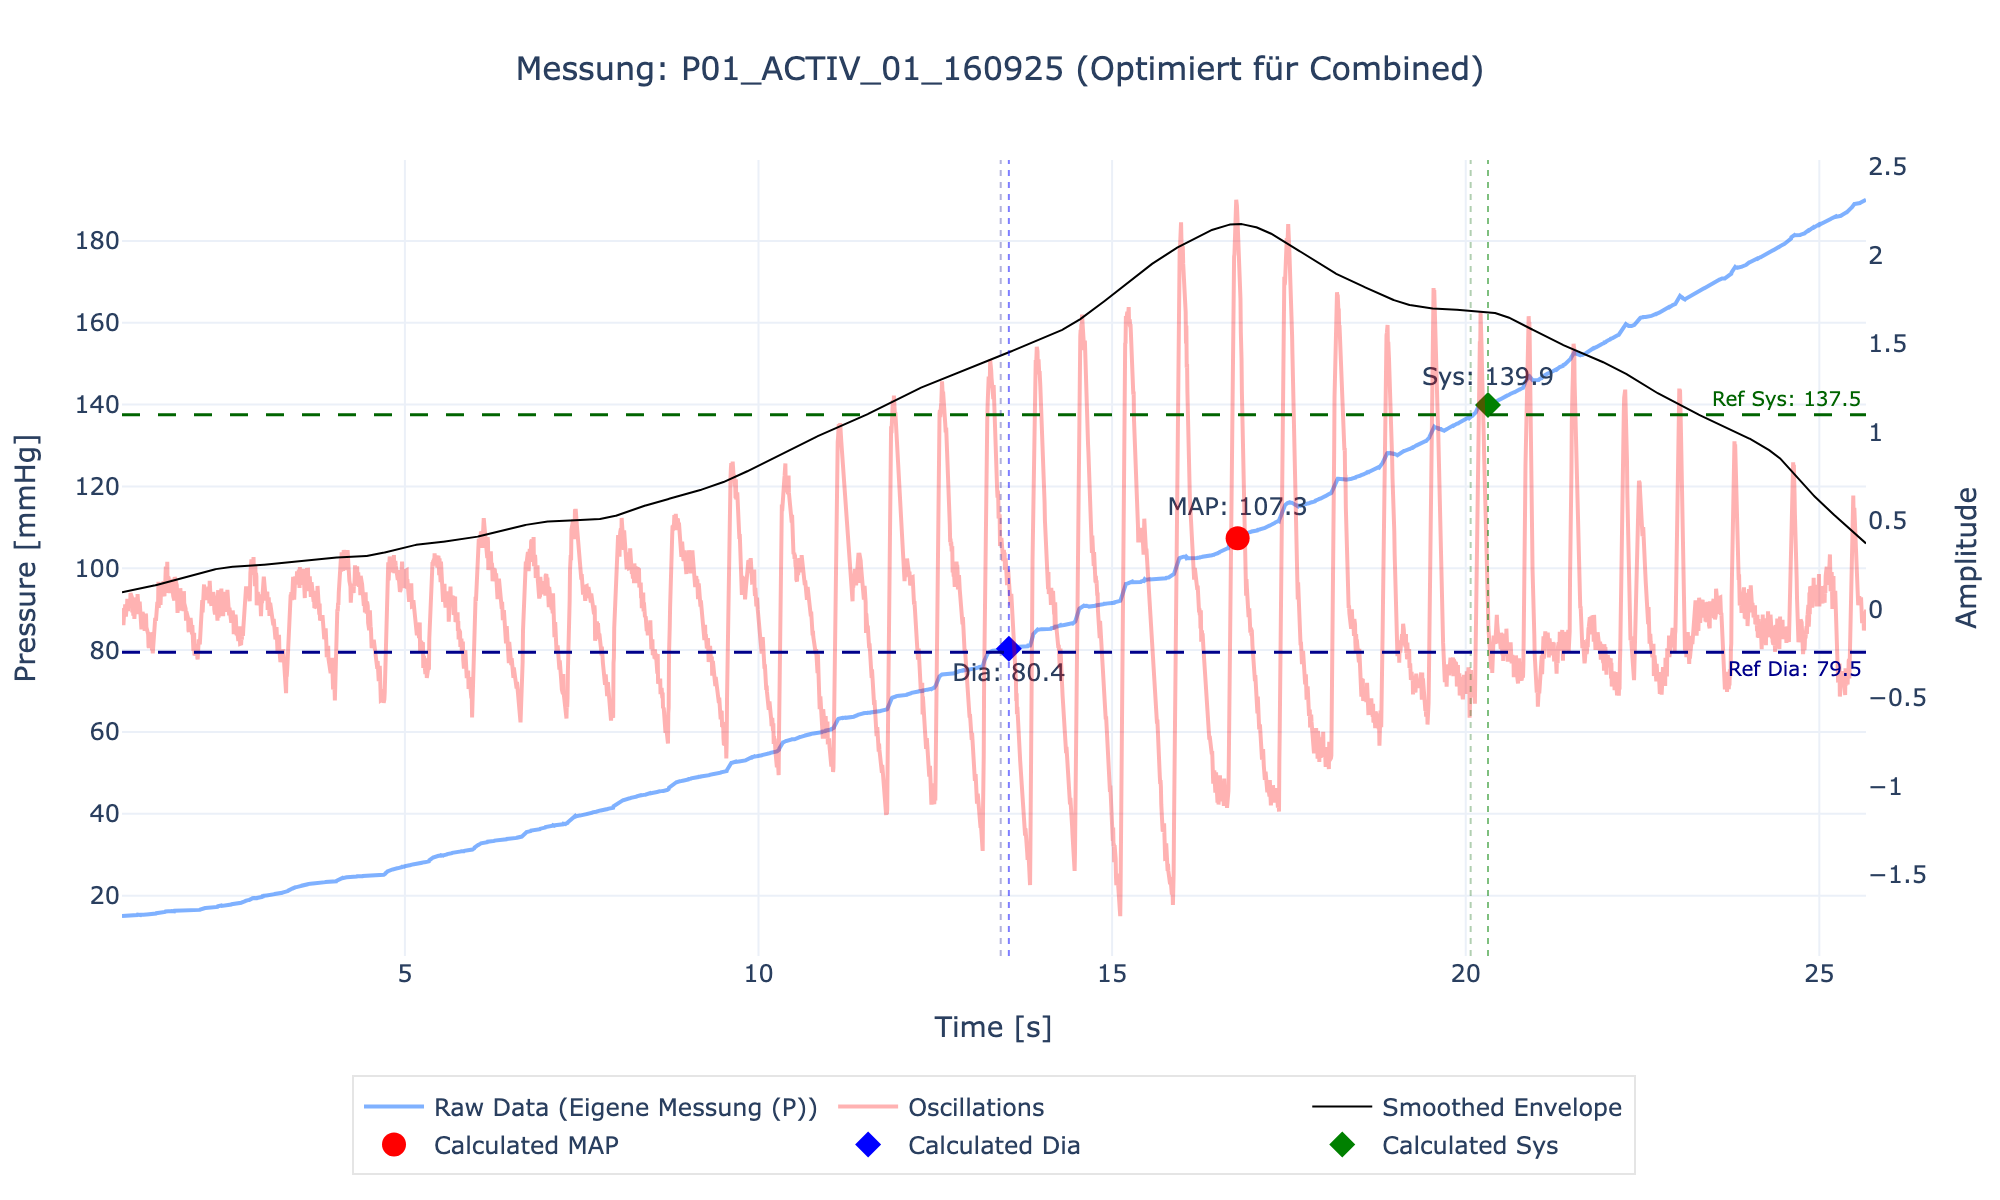
\includegraphics[width=\textwidth]{images/P01_ACTIV_01_160925_combined.png}
        \caption{Optimiert für Beurer und NAIS (Kombiniert)}
    \end{subfigure} \\
    \begin{subfigure}[b]{0.48\textwidth}
        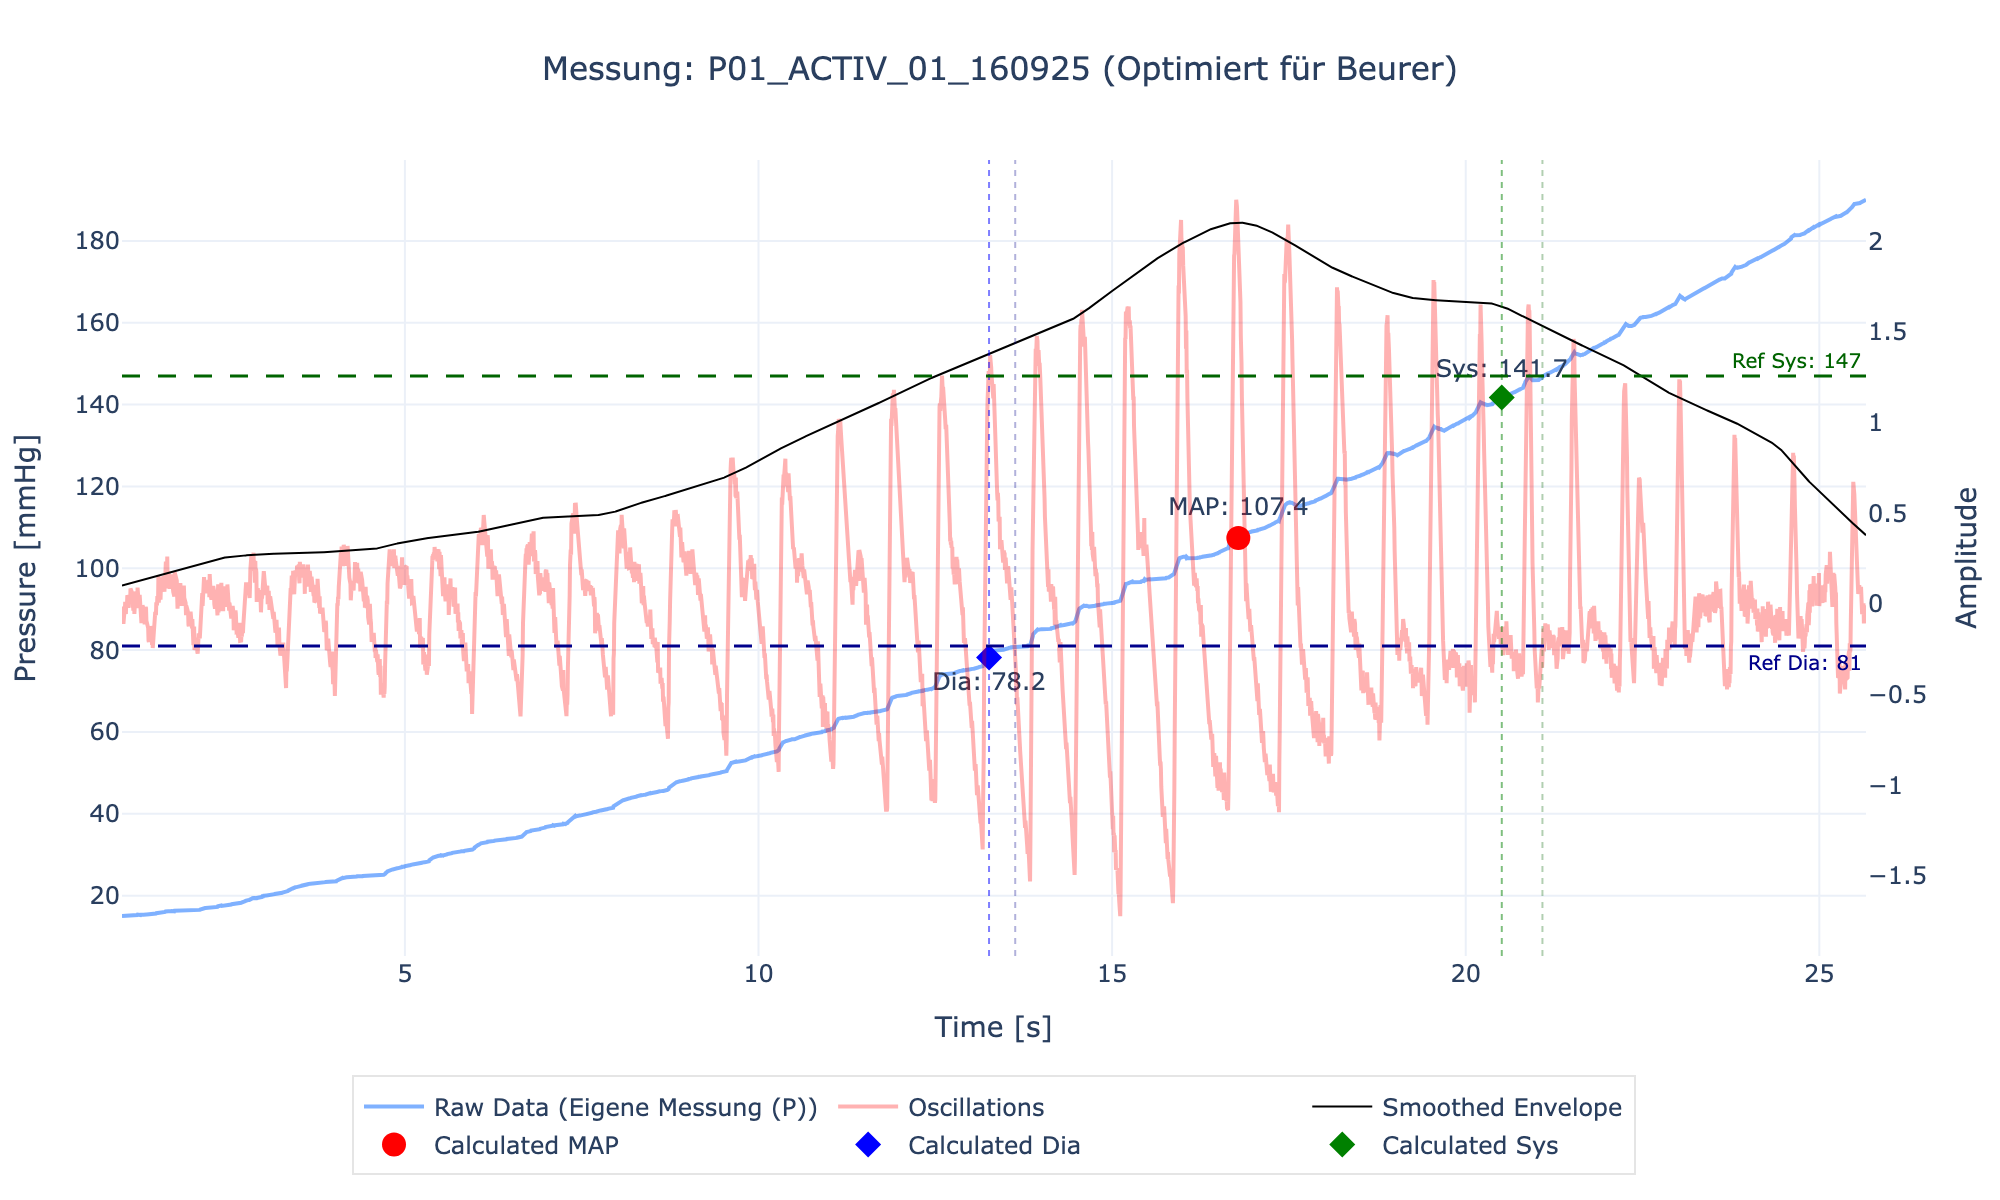
\includegraphics[width=\textwidth]{images/P01_ACTIV_01_160925_beurer.png}
        \caption{Optimiert für Beurer}
    \end{subfigure}
    \hfill
    \begin{subfigure}[b]{0.48\textwidth}
        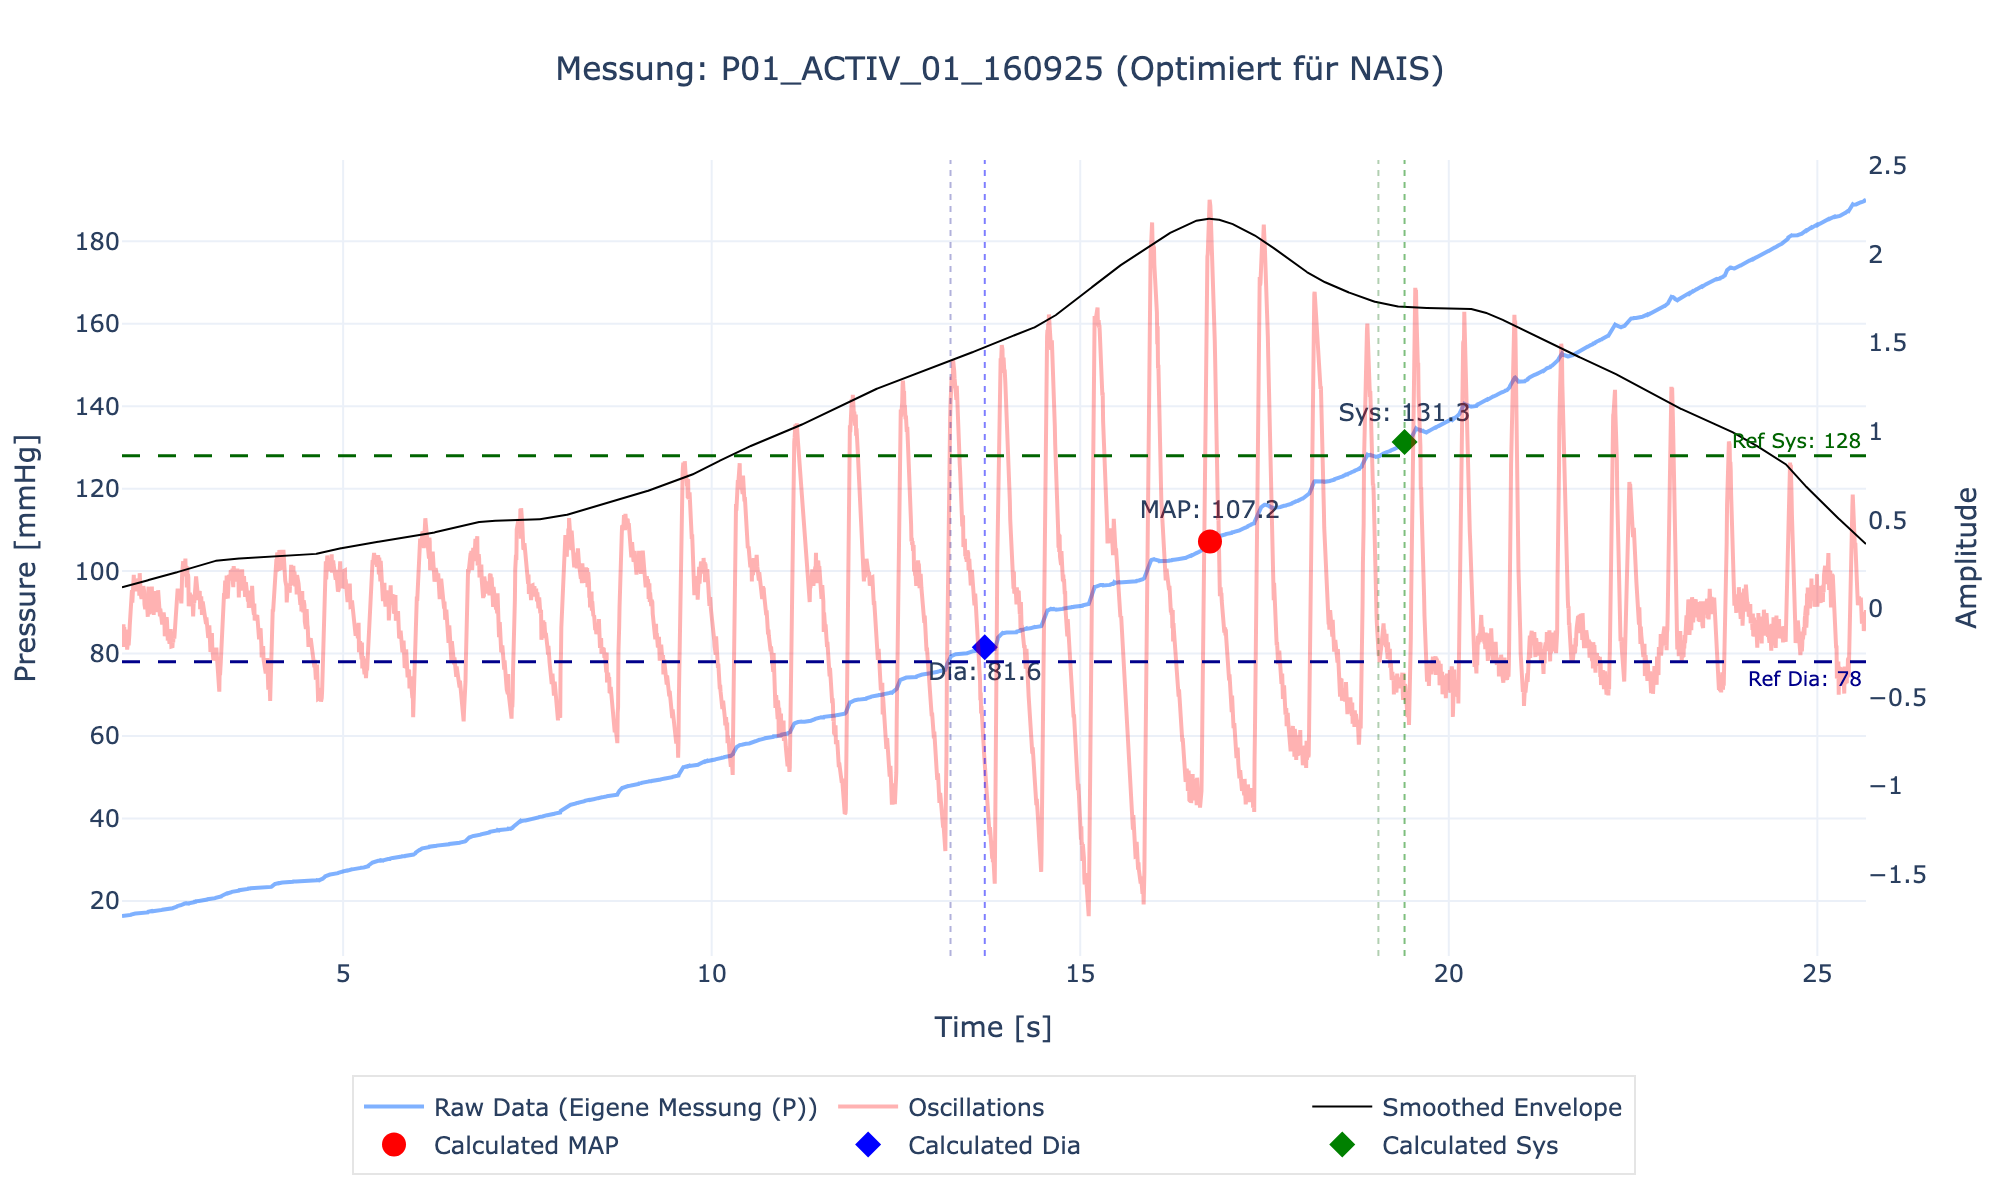
\includegraphics[width=\textwidth]{images/P01_ACTIV_01_160925_nais.png}
        \caption{Optimiert für NAIS}
    \end{subfigure}
    \caption{Einzelauswertung der Messung P01\_ACTIV\_01\_160925 mit verschiedenen Parametersätzen.}
\end{figure}
\newpage

\subsection*{Messung: P01\_REST\_01\_100825}
\begin{figure}[H]
    \centering
    \begin{subfigure}[b]{0.8\textwidth}
        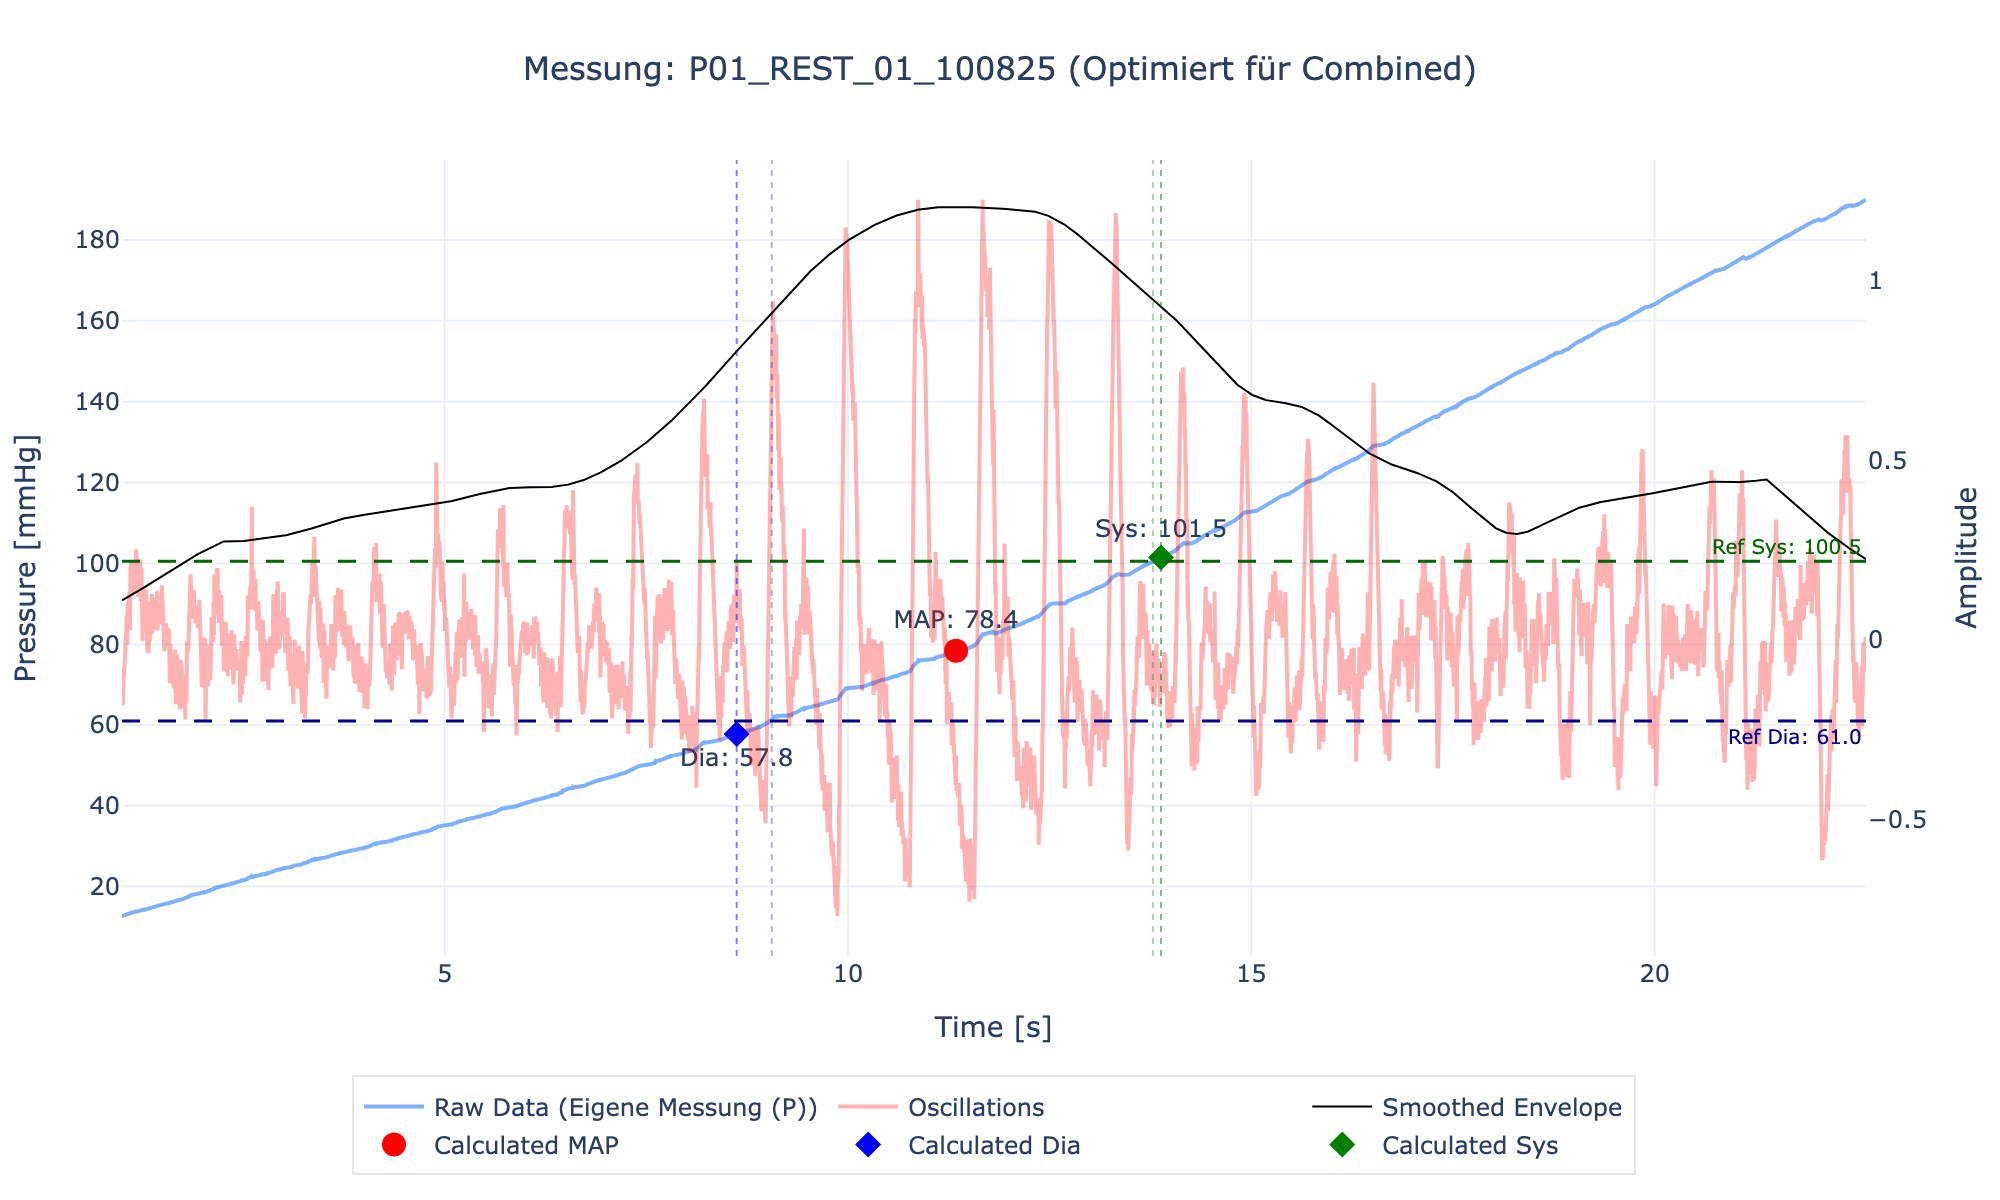
\includegraphics[width=\textwidth]{images/P01_REST_01_100825_combined.png}
        \caption{Optimiert für Beurer und NAIS (Kombiniert)}
    \end{subfigure} \\
    \begin{subfigure}[b]{0.48\textwidth}
        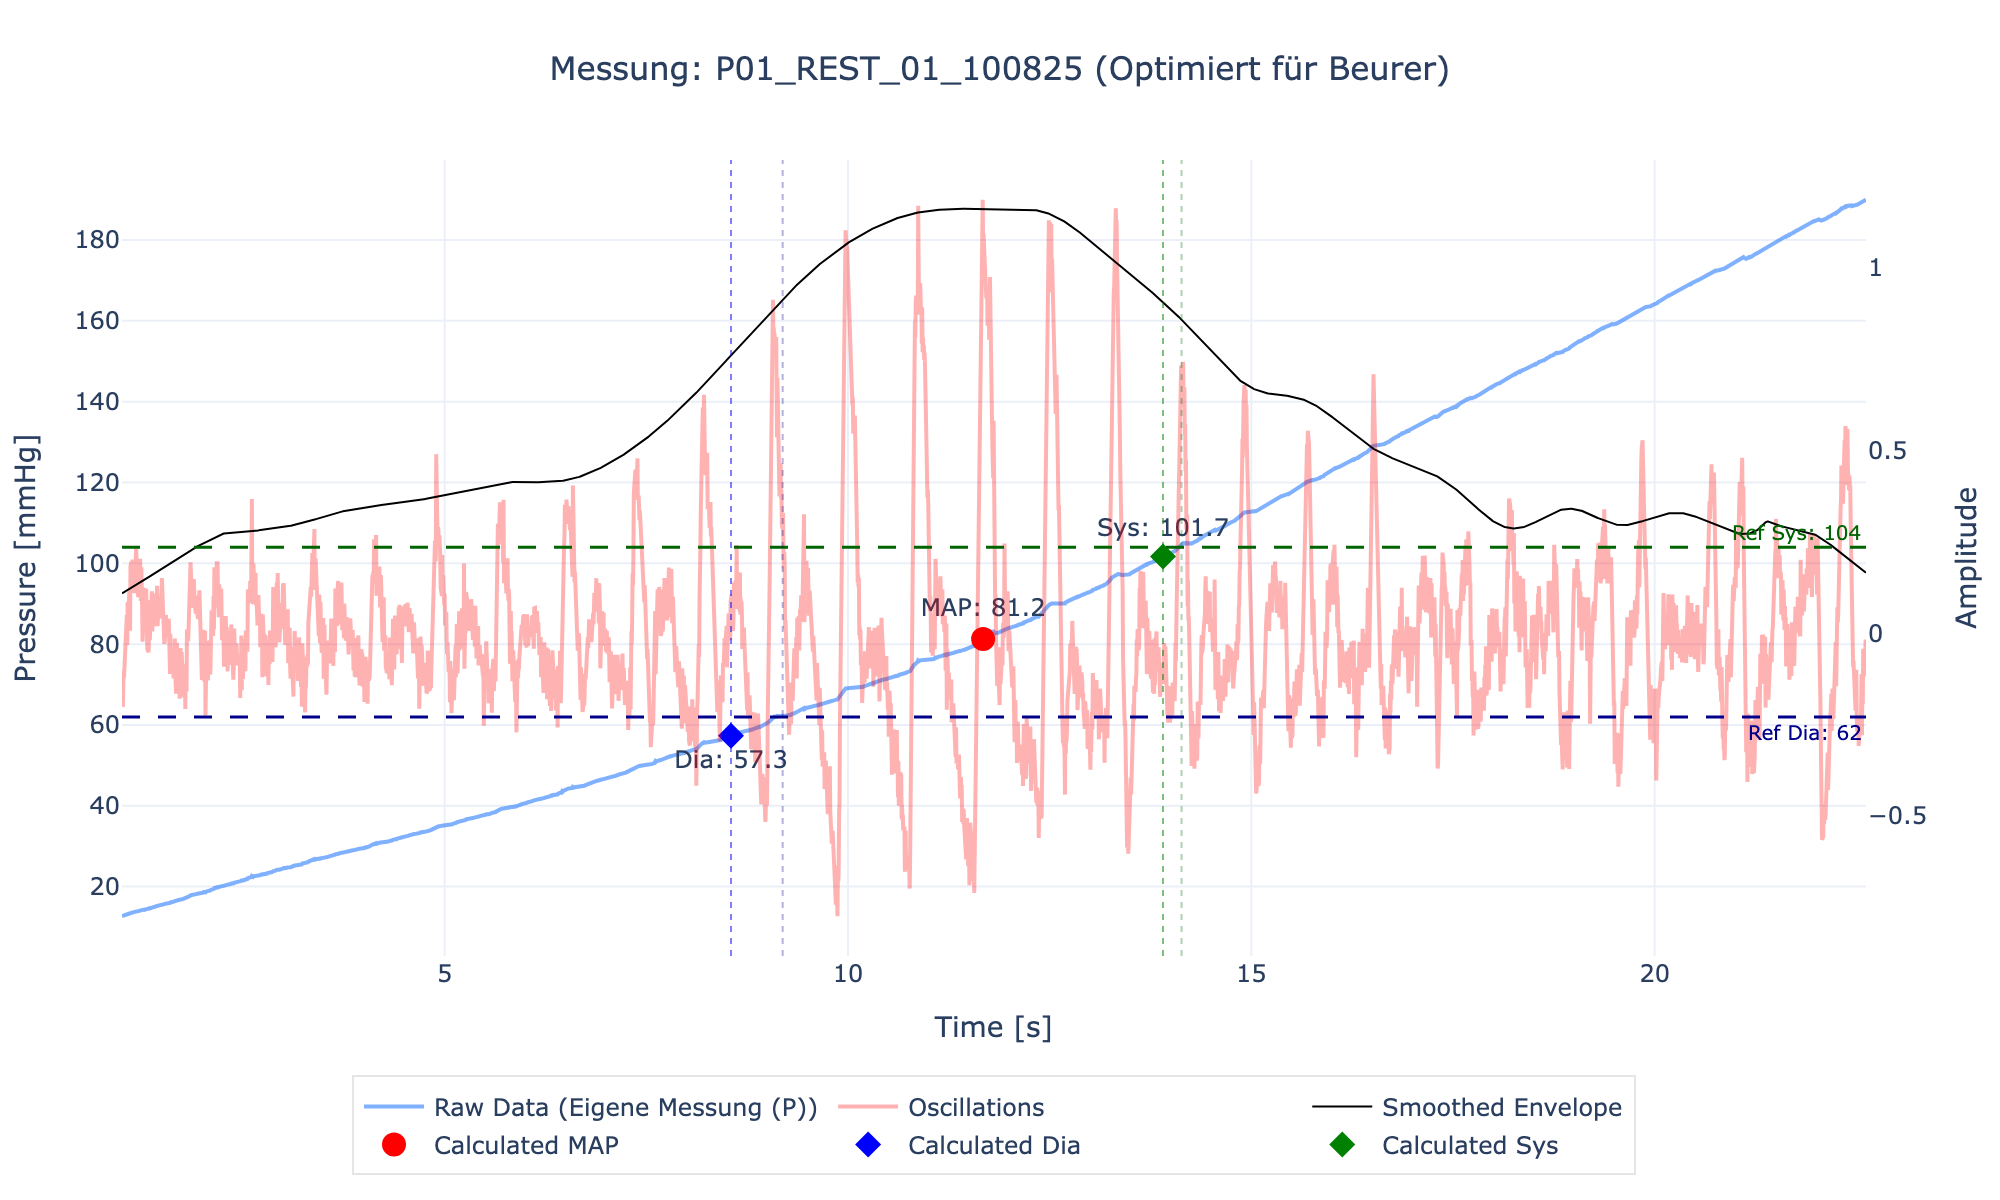
\includegraphics[width=\textwidth]{images/P01_REST_01_100825_beurer.png}
        \caption{Optimiert für Beurer}
    \end{subfigure}
    \hfill
    \begin{subfigure}[b]{0.48\textwidth}
        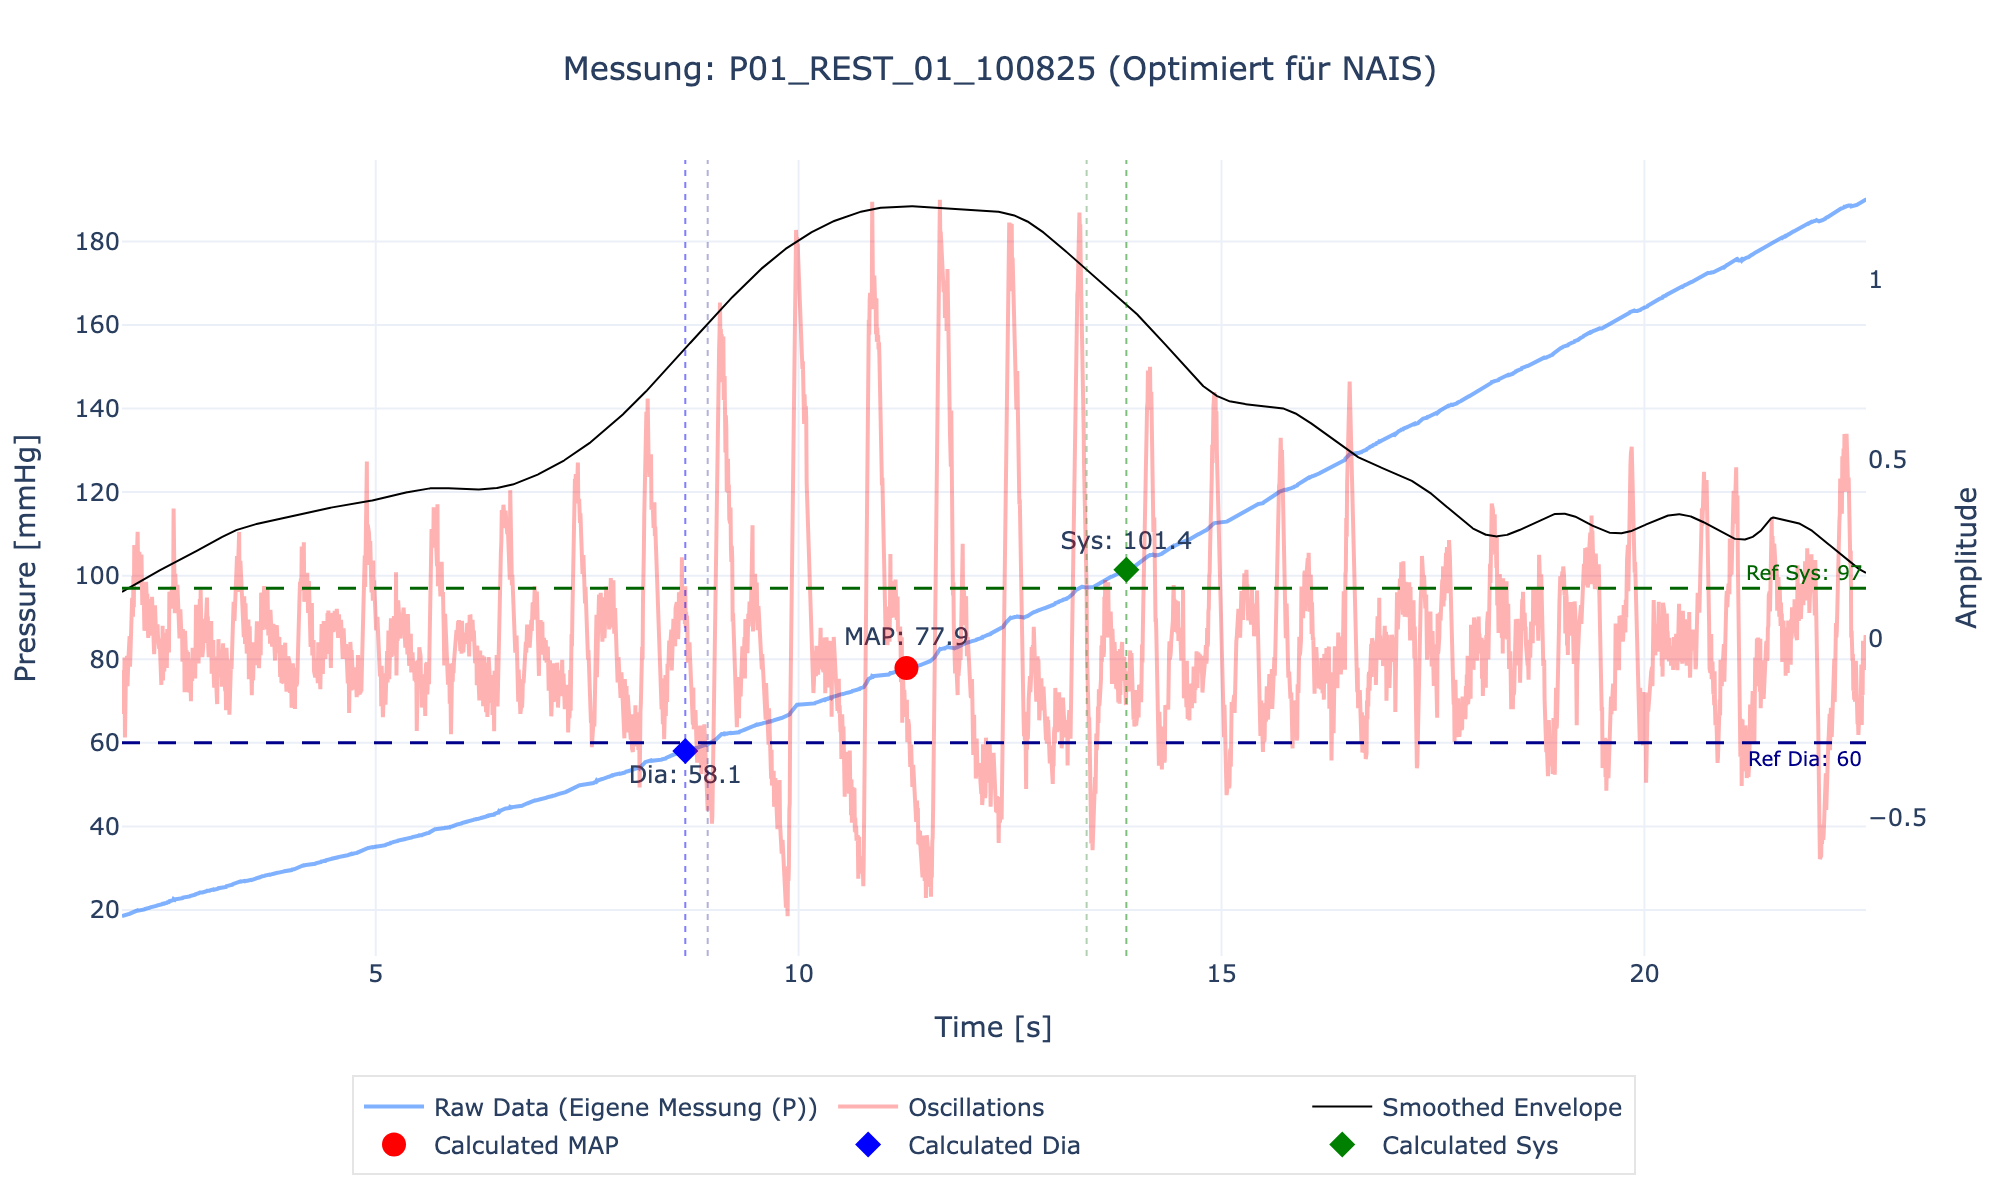
\includegraphics[width=\textwidth]{images/P01_REST_01_100825_nais.png}
        \caption{Optimiert für NAIS}
    \end{subfigure}
    \caption{Einzelauswertung der Messung P01\_REST\_01\_100825 mit verschiedenen Parametersätzen.}
\end{figure}
\newpage

\subsection*{Messung: P01\_REST\_02\_100825}
\begin{figure}[H]
    \centering
    \begin{subfigure}[b]{0.8\textwidth}
        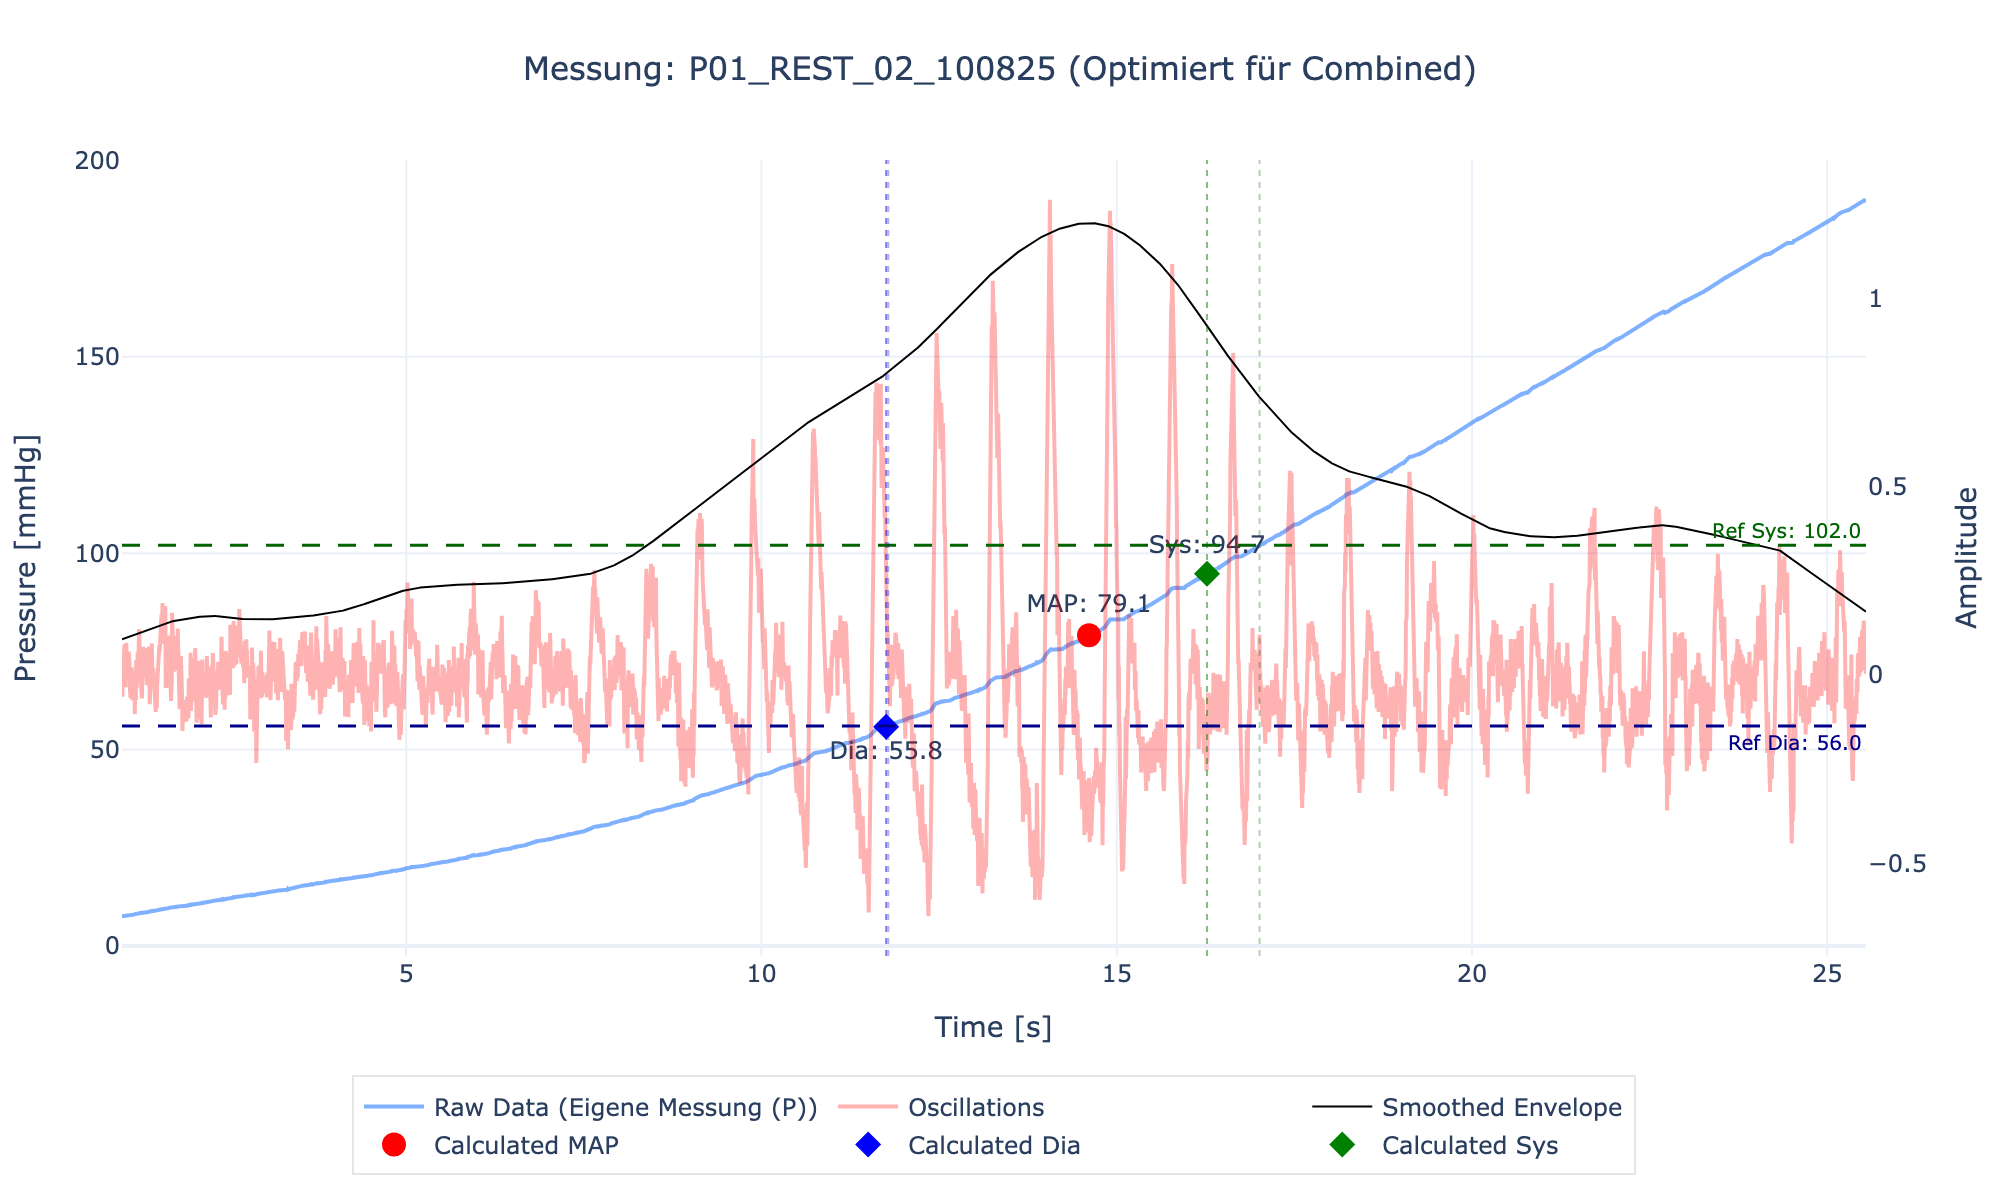
\includegraphics[width=\textwidth]{images/P01_REST_02_100825_combined.png}
        \caption{Optimiert für Beurer und NAIS (Kombiniert)}
    \end{subfigure} \\
    \begin{subfigure}[b]{0.48\textwidth}
        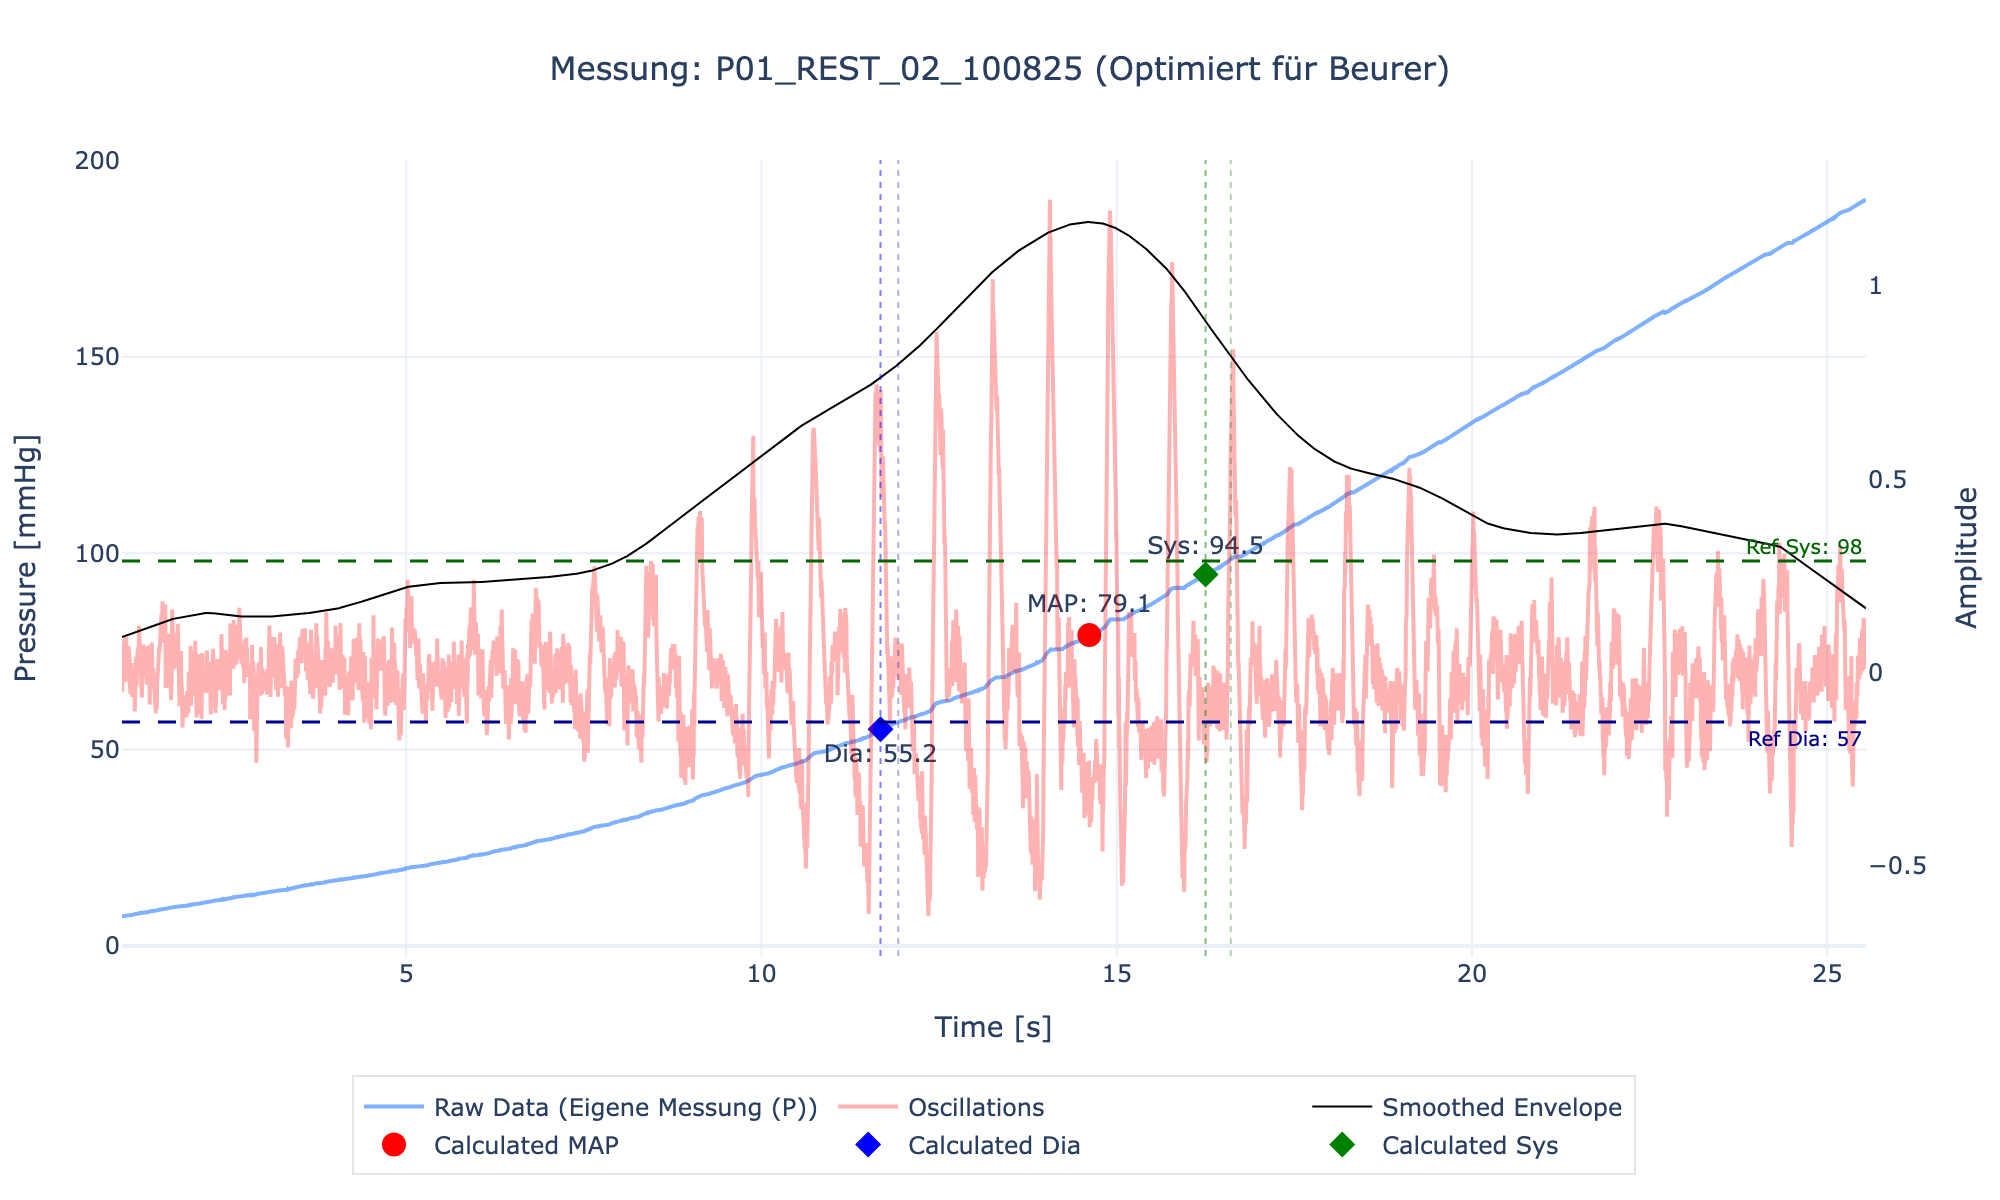
\includegraphics[width=\textwidth]{images/P01_REST_02_100825_beurer.png}
        \caption{Optimiert für Beurer}
    \end{subfigure}
    \hfill
    \begin{subfigure}[b]{0.48\textwidth}
        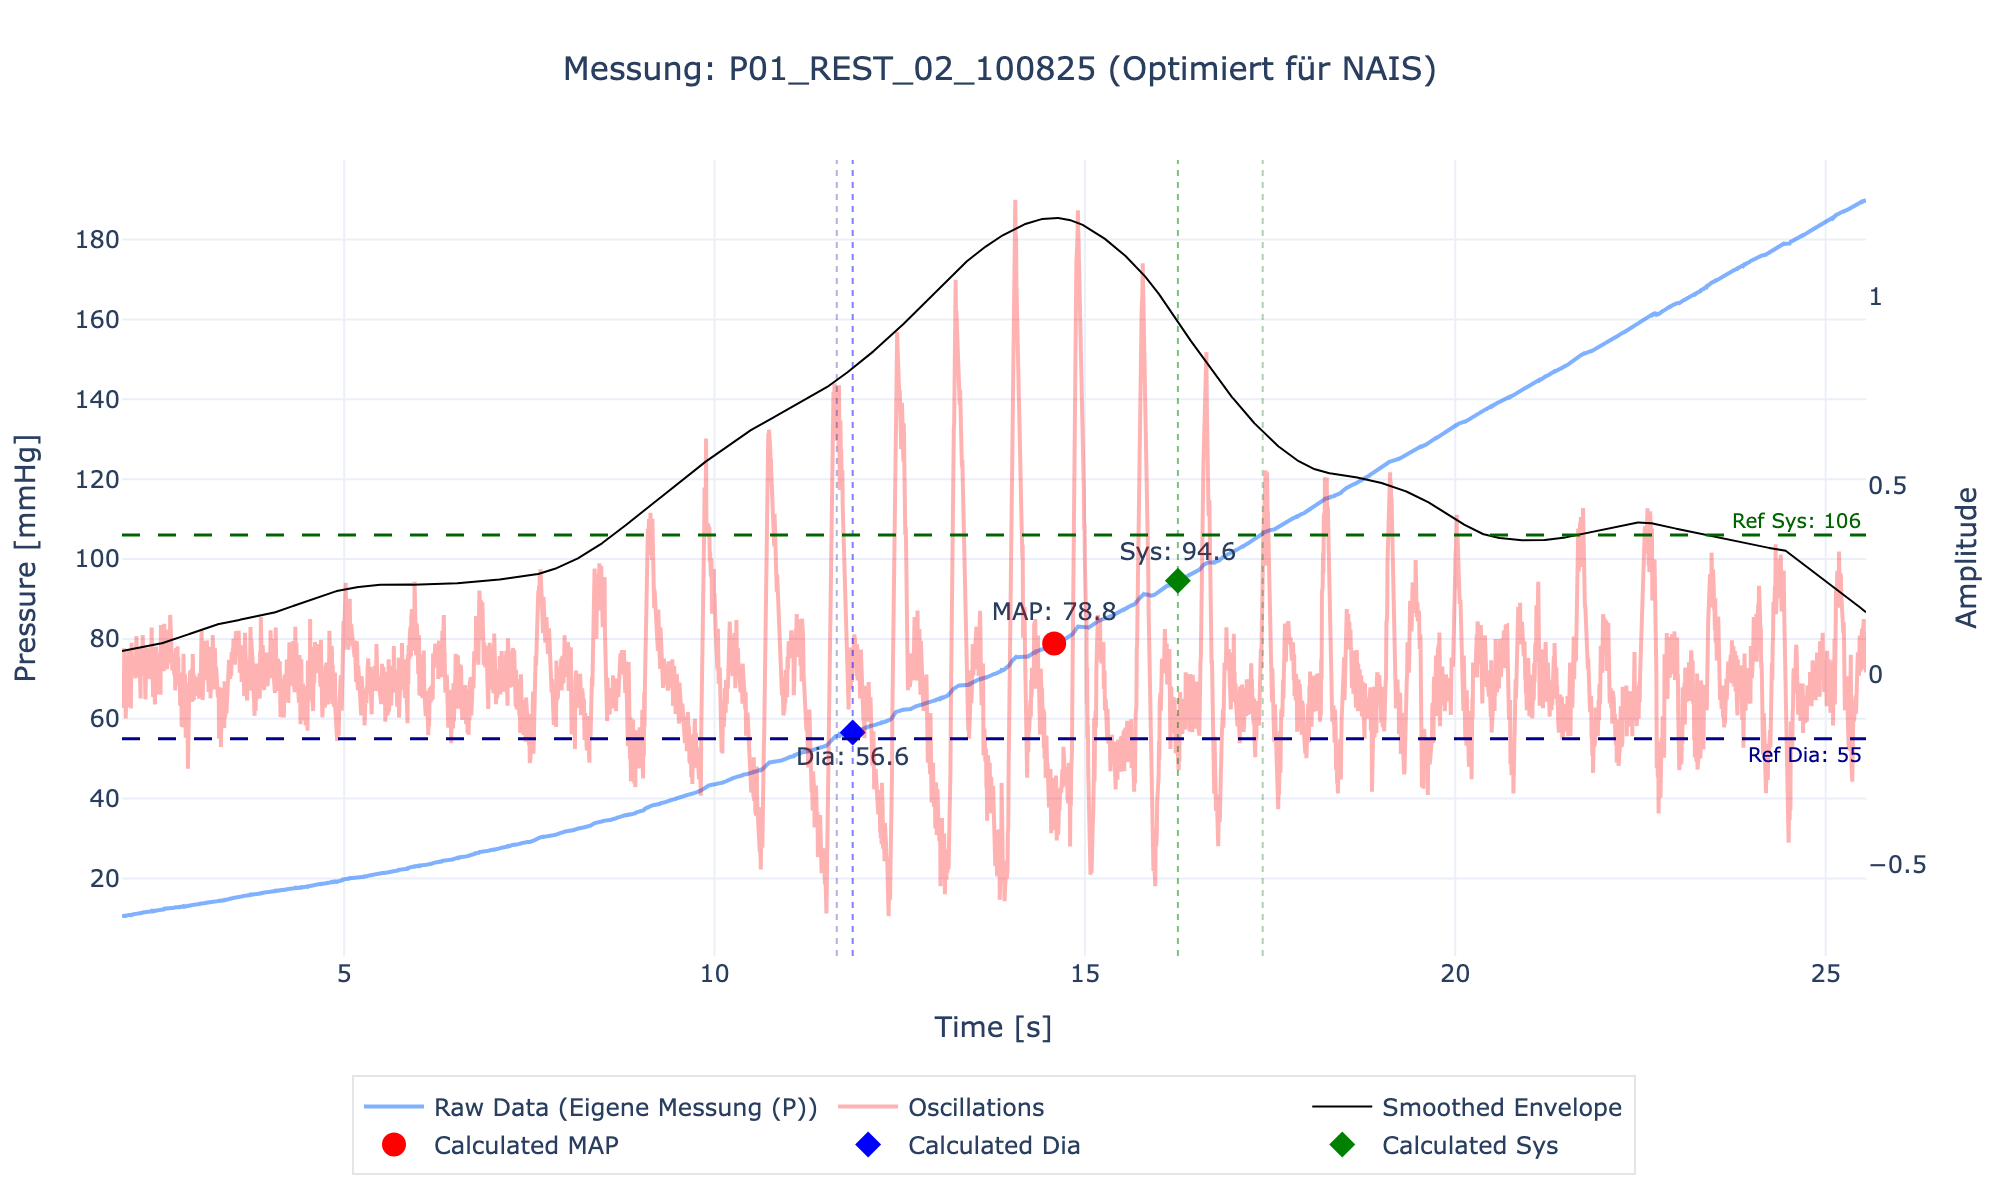
\includegraphics[width=\textwidth]{images/P01_REST_02_100825_nais.png}
        \caption{Optimiert für NAIS}
    \end{subfigure}
    \caption{Einzelauswertung der Messung P01\_REST\_02\_100825 mit verschiedenen Parametersätzen.}
\end{figure}
\newpage

\subsection*{Messung: P02\_ACTIV\_01\_160925}
\begin{figure}[H]
    \centering
    \begin{subfigure}[b]{0.8\textwidth}
        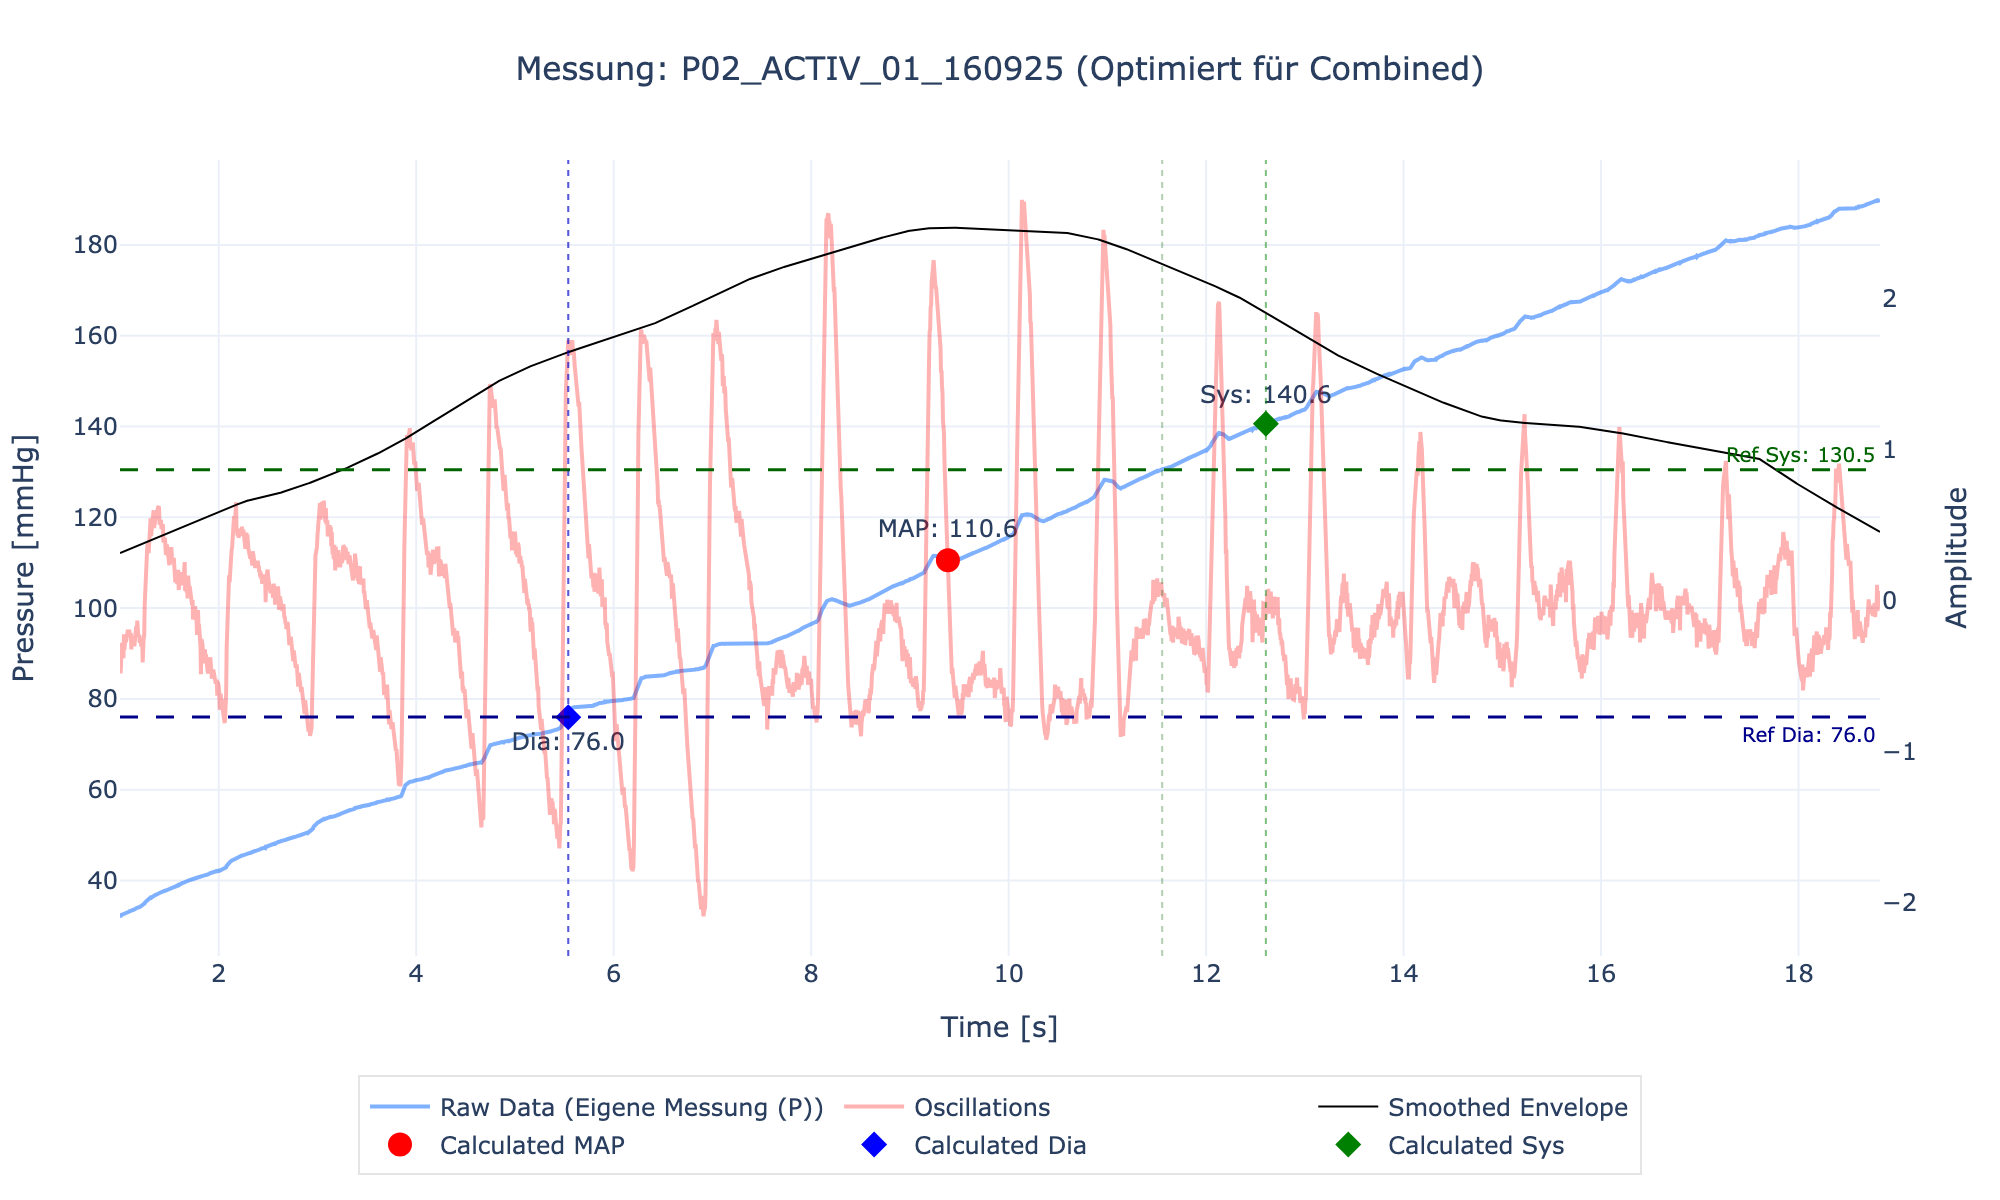
\includegraphics[width=\textwidth]{images/P02_ACTIV_01_160925_combined.png}
        \caption{Optimiert für Beurer und NAIS (Kombiniert)}
    \end{subfigure} \\
    \begin{subfigure}[b]{0.48\textwidth}
        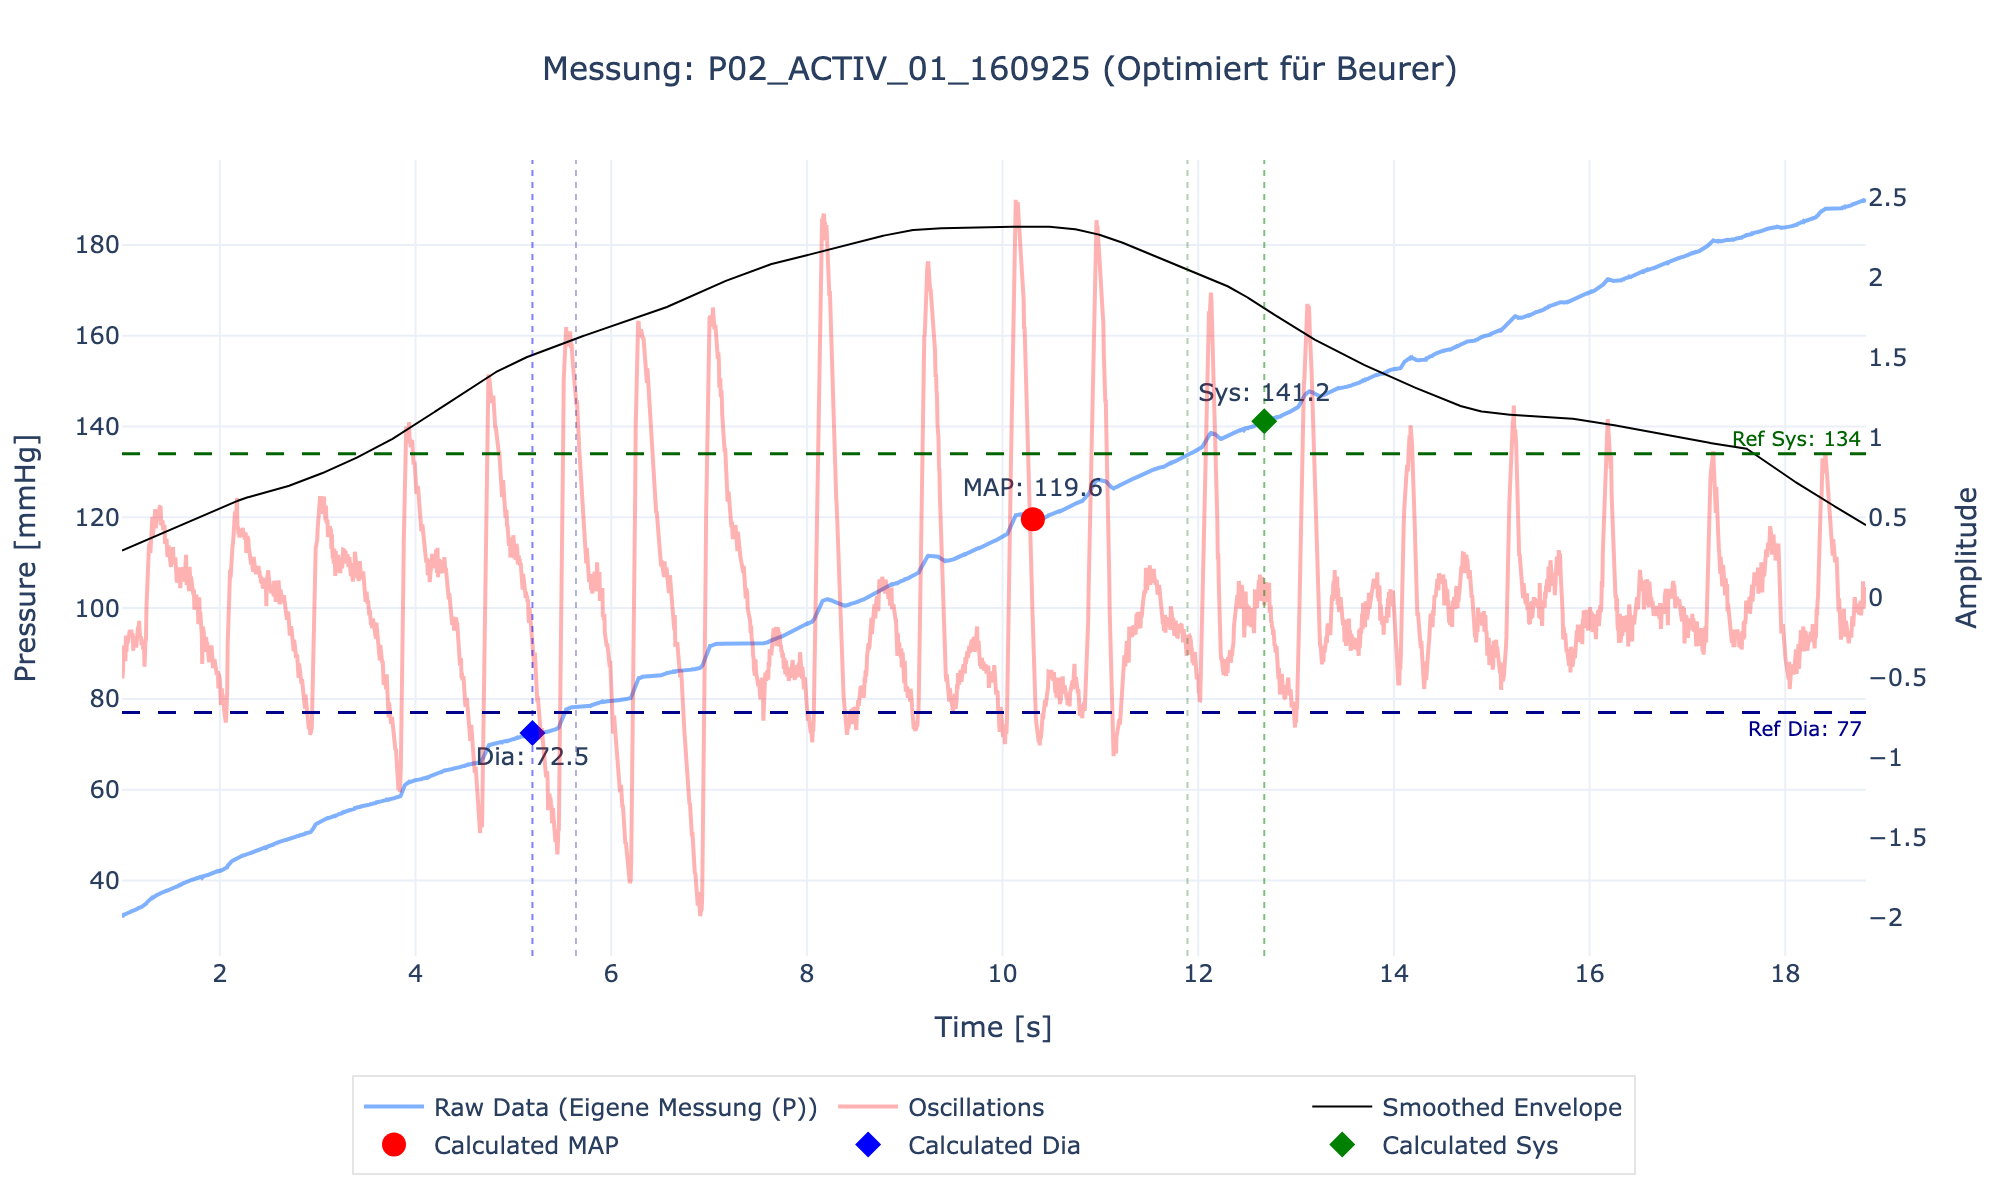
\includegraphics[width=\textwidth]{images/P02_ACTIV_01_160925_beurer.png}
        \caption{Optimiert für Beurer}
    \end{subfigure}
    \hfill
    \begin{subfigure}[b]{0.48\textwidth}
        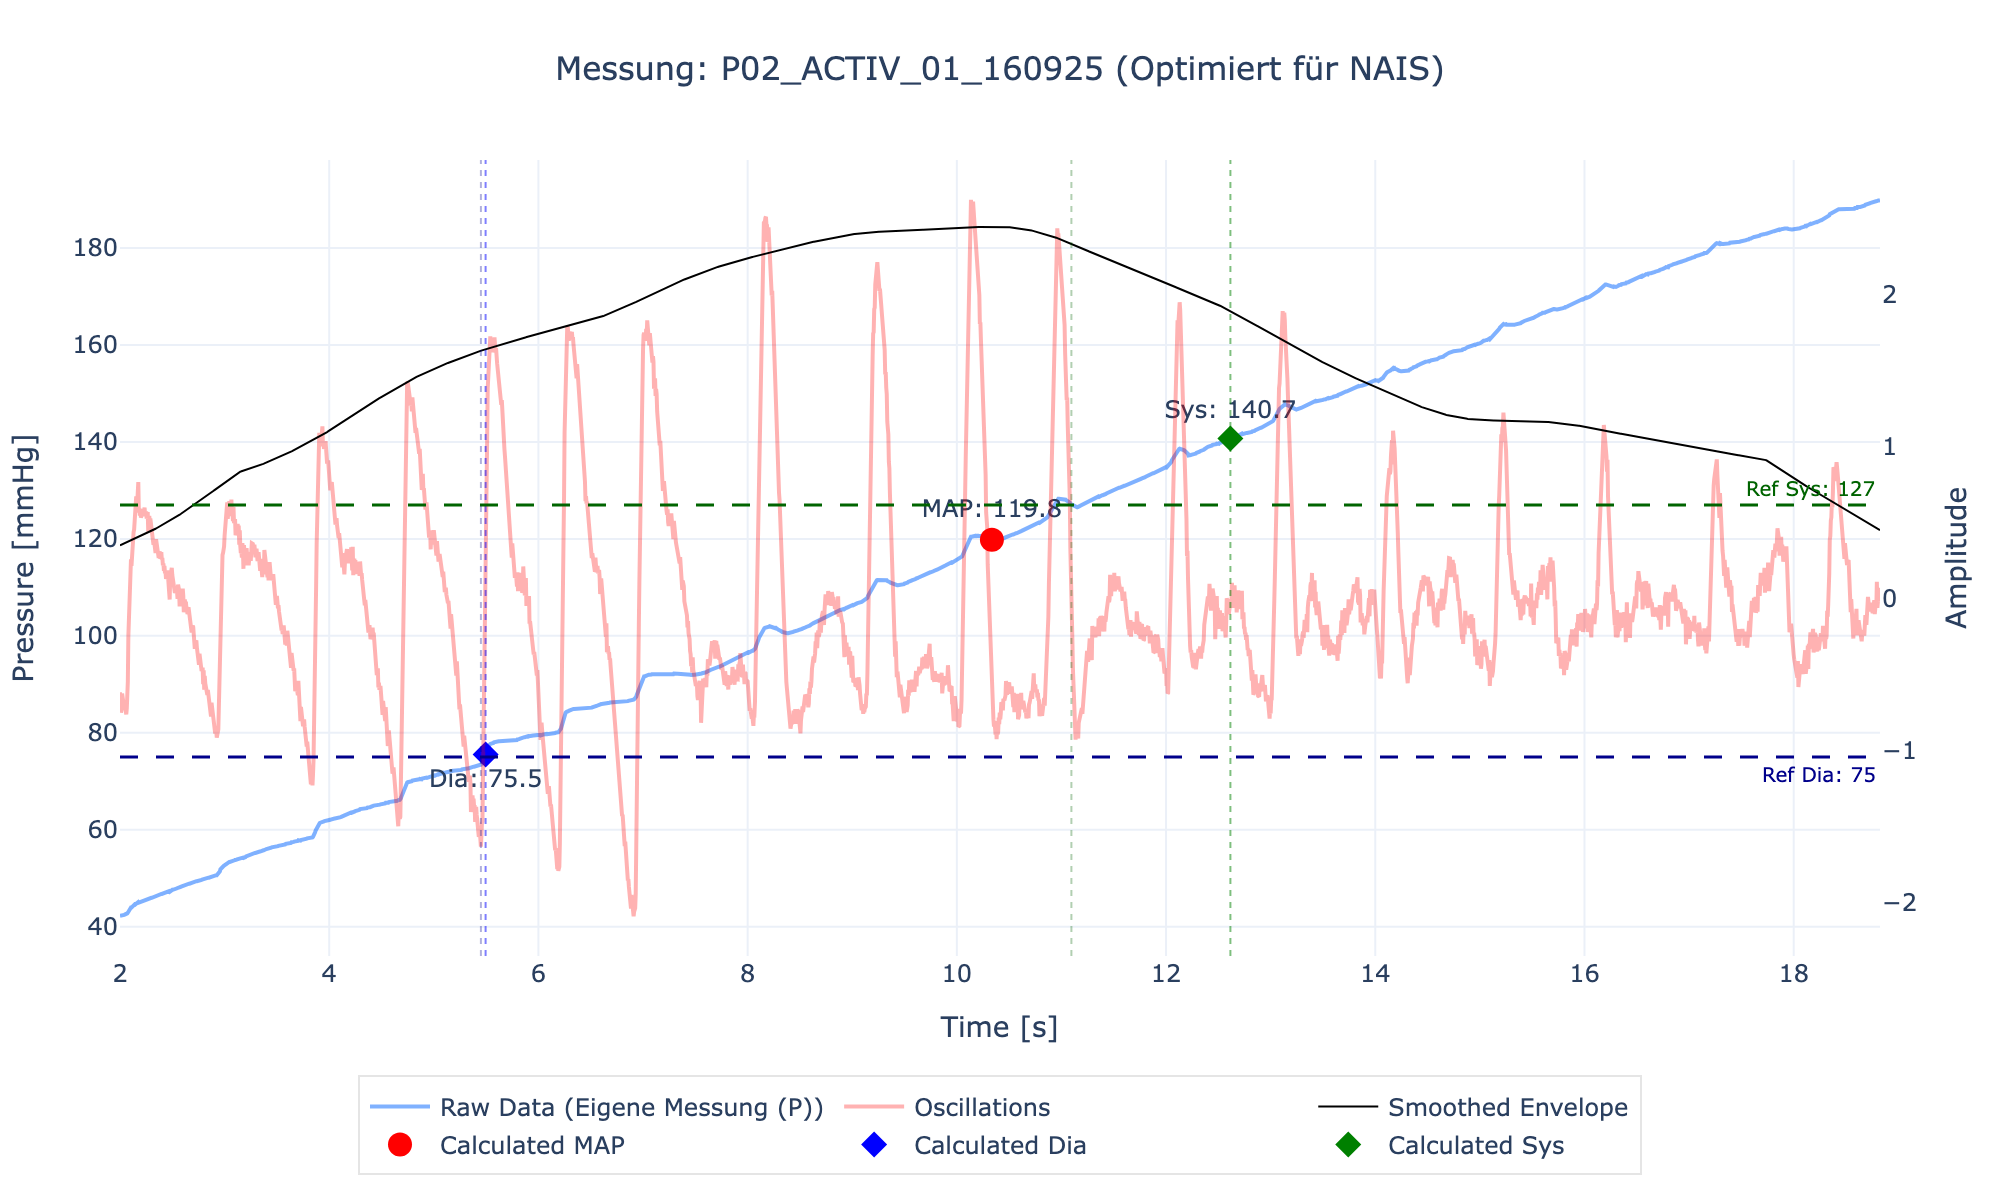
\includegraphics[width=\textwidth]{images/P02_ACTIV_01_160925_nais.png}
        \caption{Optimiert für NAIS}
    \end{subfigure}
    \caption{Einzelauswertung der Messung P02\_ACTIV\_01\_160925 mit verschiedenen Parametersätzen.}
\end{figure}
\newpage

\subsection*{Messung: P02\_REST\_01\_100825}
\begin{figure}[H]
    \centering
    \begin{subfigure}[b]{0.8\textwidth}
        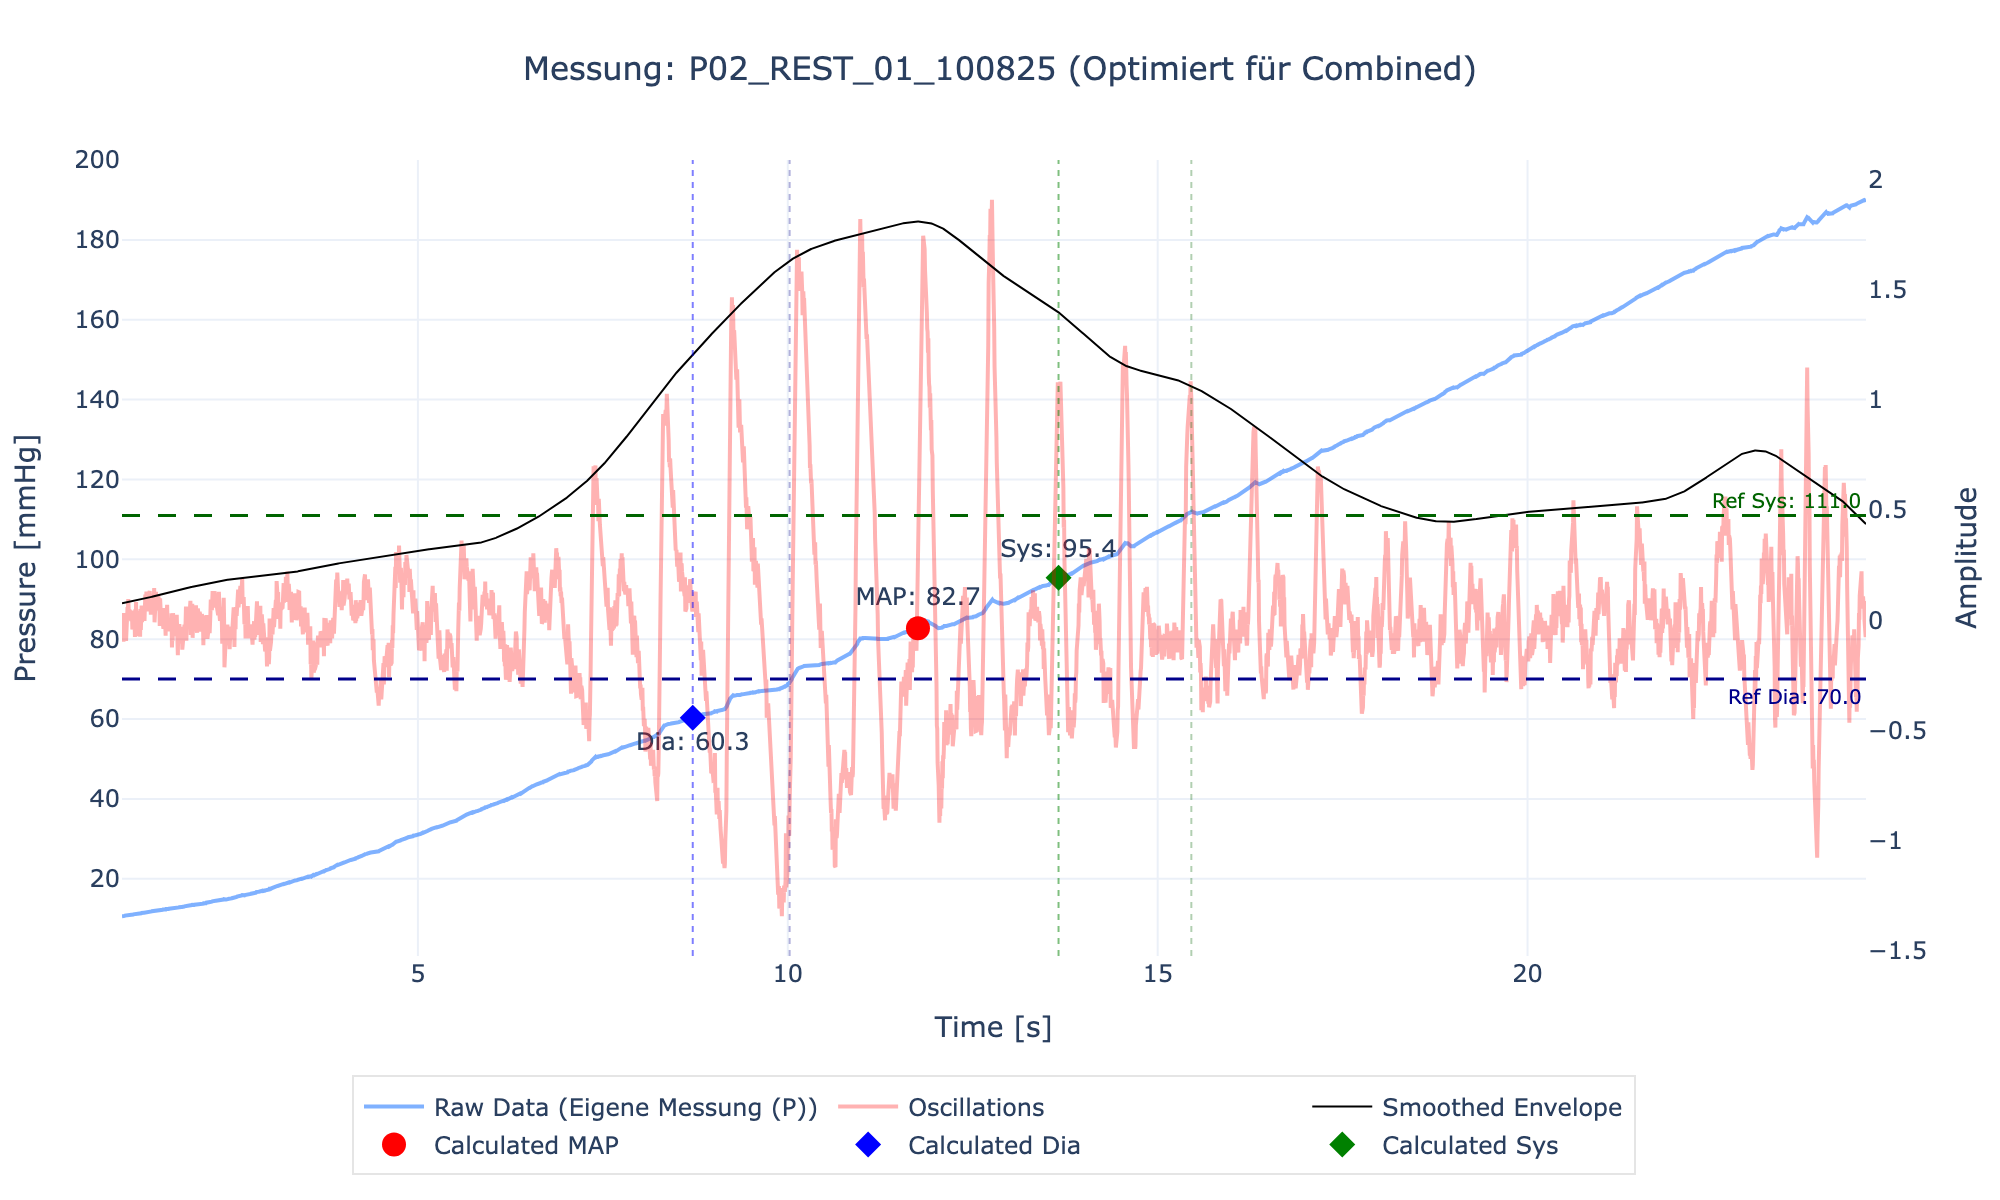
\includegraphics[width=\textwidth]{images/P02_REST_01_100825_combined.png}
        \caption{Optimiert für Beurer und NAIS (Kombiniert)}
    \end{subfigure} \\
    \begin{subfigure}[b]{0.48\textwidth}
        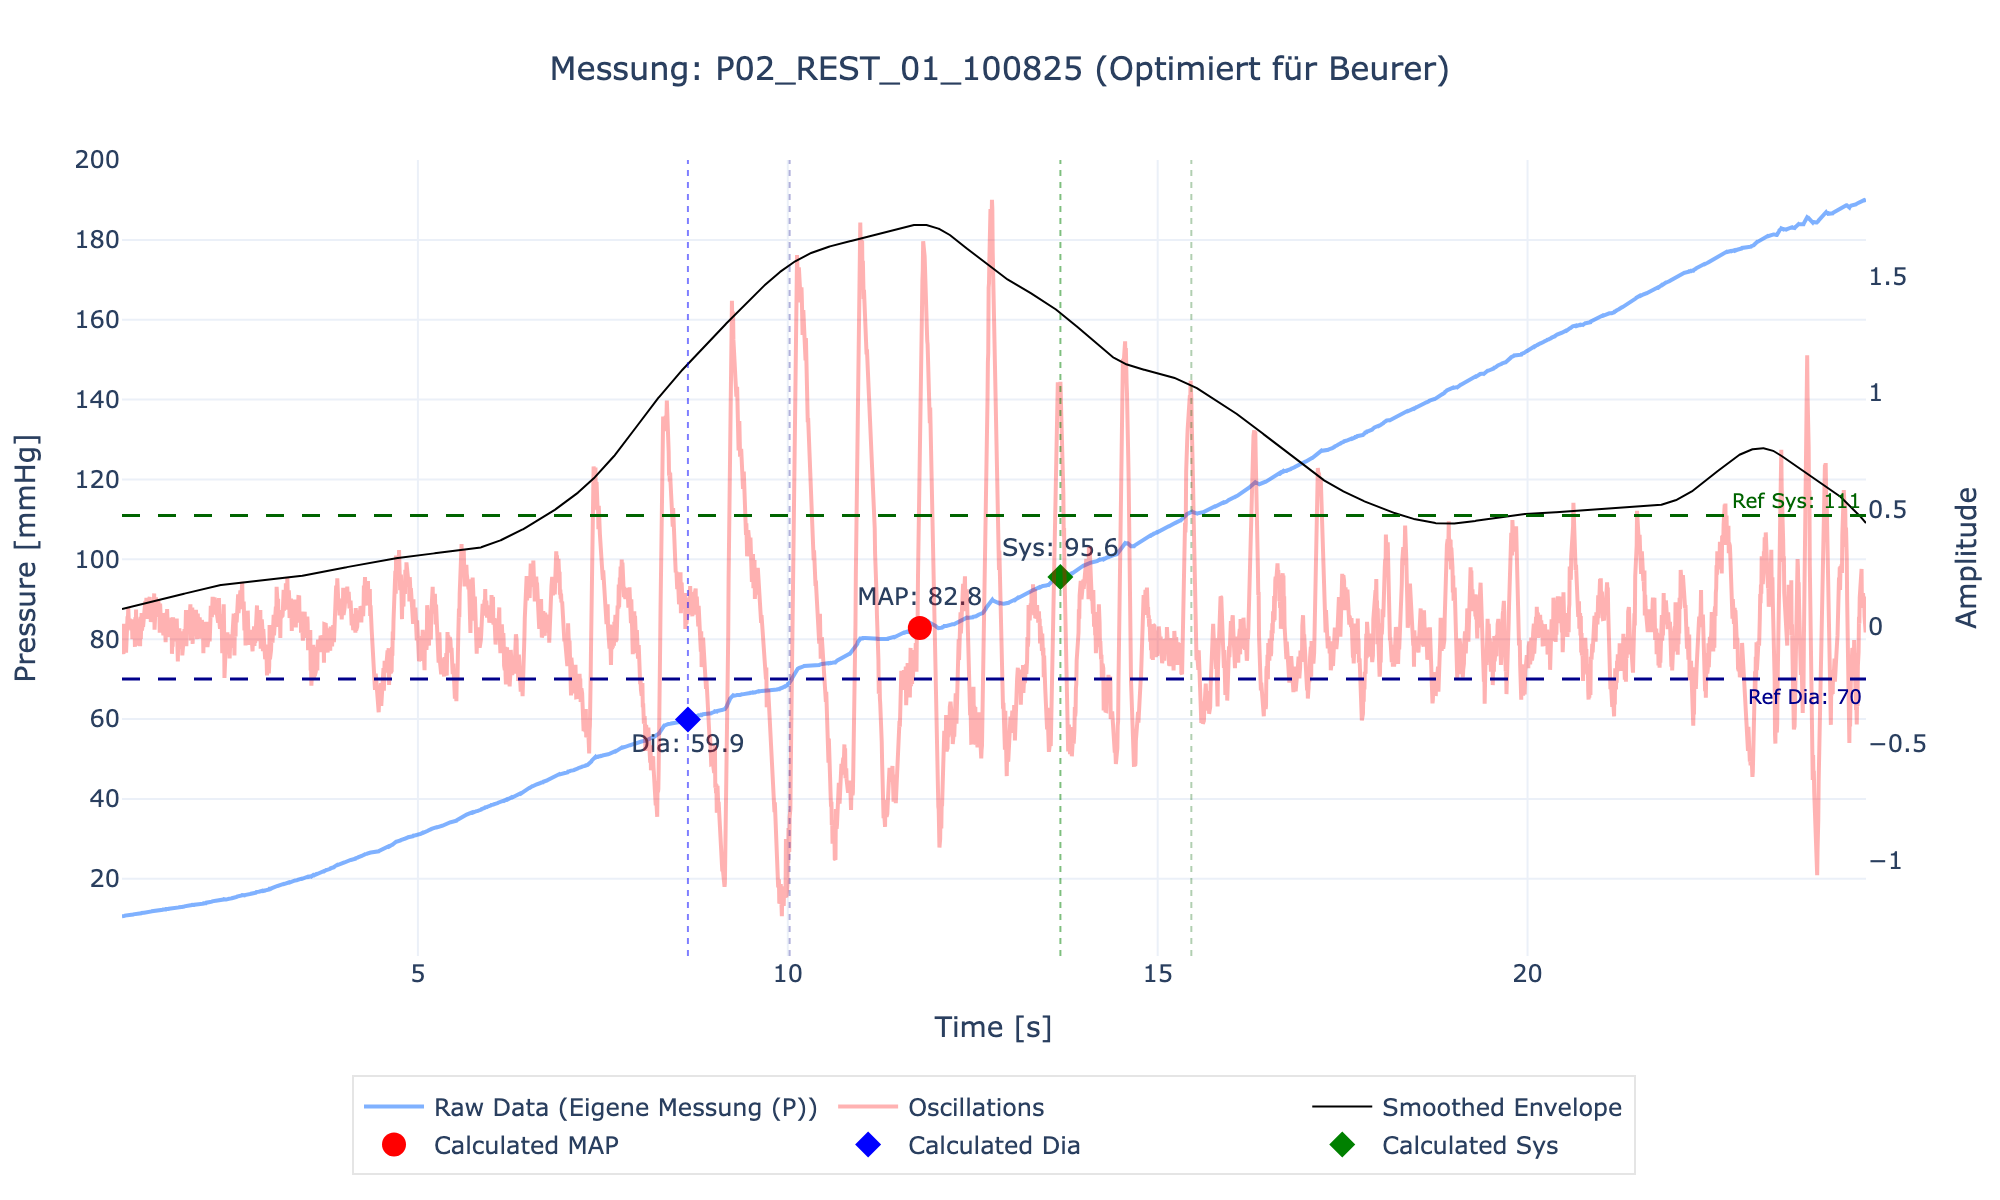
\includegraphics[width=\textwidth]{images/P02_REST_01_100825_beurer.png}
        \caption{Optimiert für Beurer}
    \end{subfigure}
    \hfill
    \begin{subfigure}[b]{0.48\textwidth}
        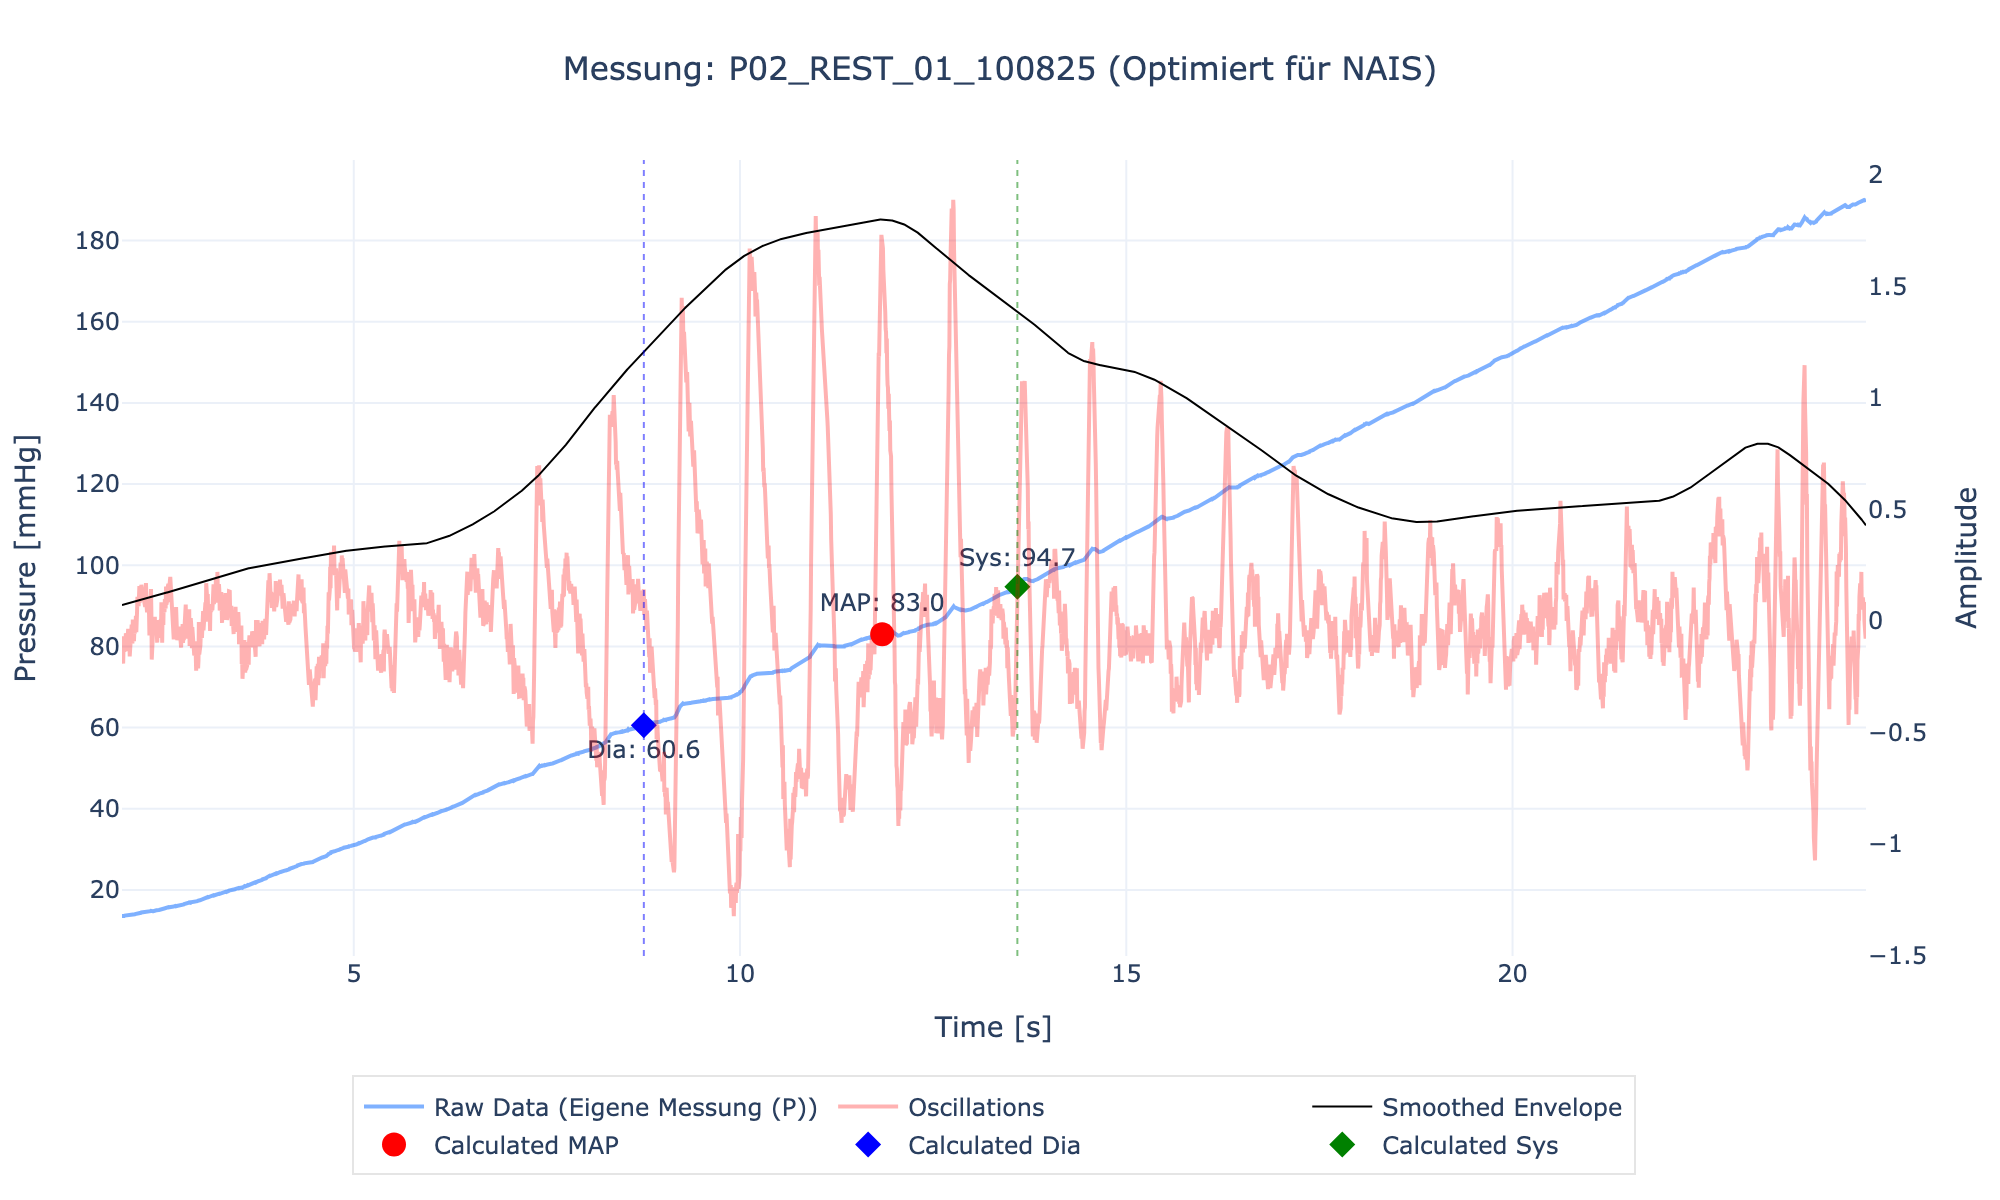
\includegraphics[width=\textwidth]{images/P02_REST_01_100825_nais.png}
        \caption{Optimiert für NAIS}
    \end{subfigure}
    \caption{Einzelauswertung der Messung P02\_REST\_01\_100825 mit verschiedenen Parametersätzen.}
\end{figure}
\newpage

\subsection*{Messung: P02\_REST\_02\_160925}
\begin{figure}[H]
    \centering
    \begin{subfigure}[b]{0.8\textwidth}
        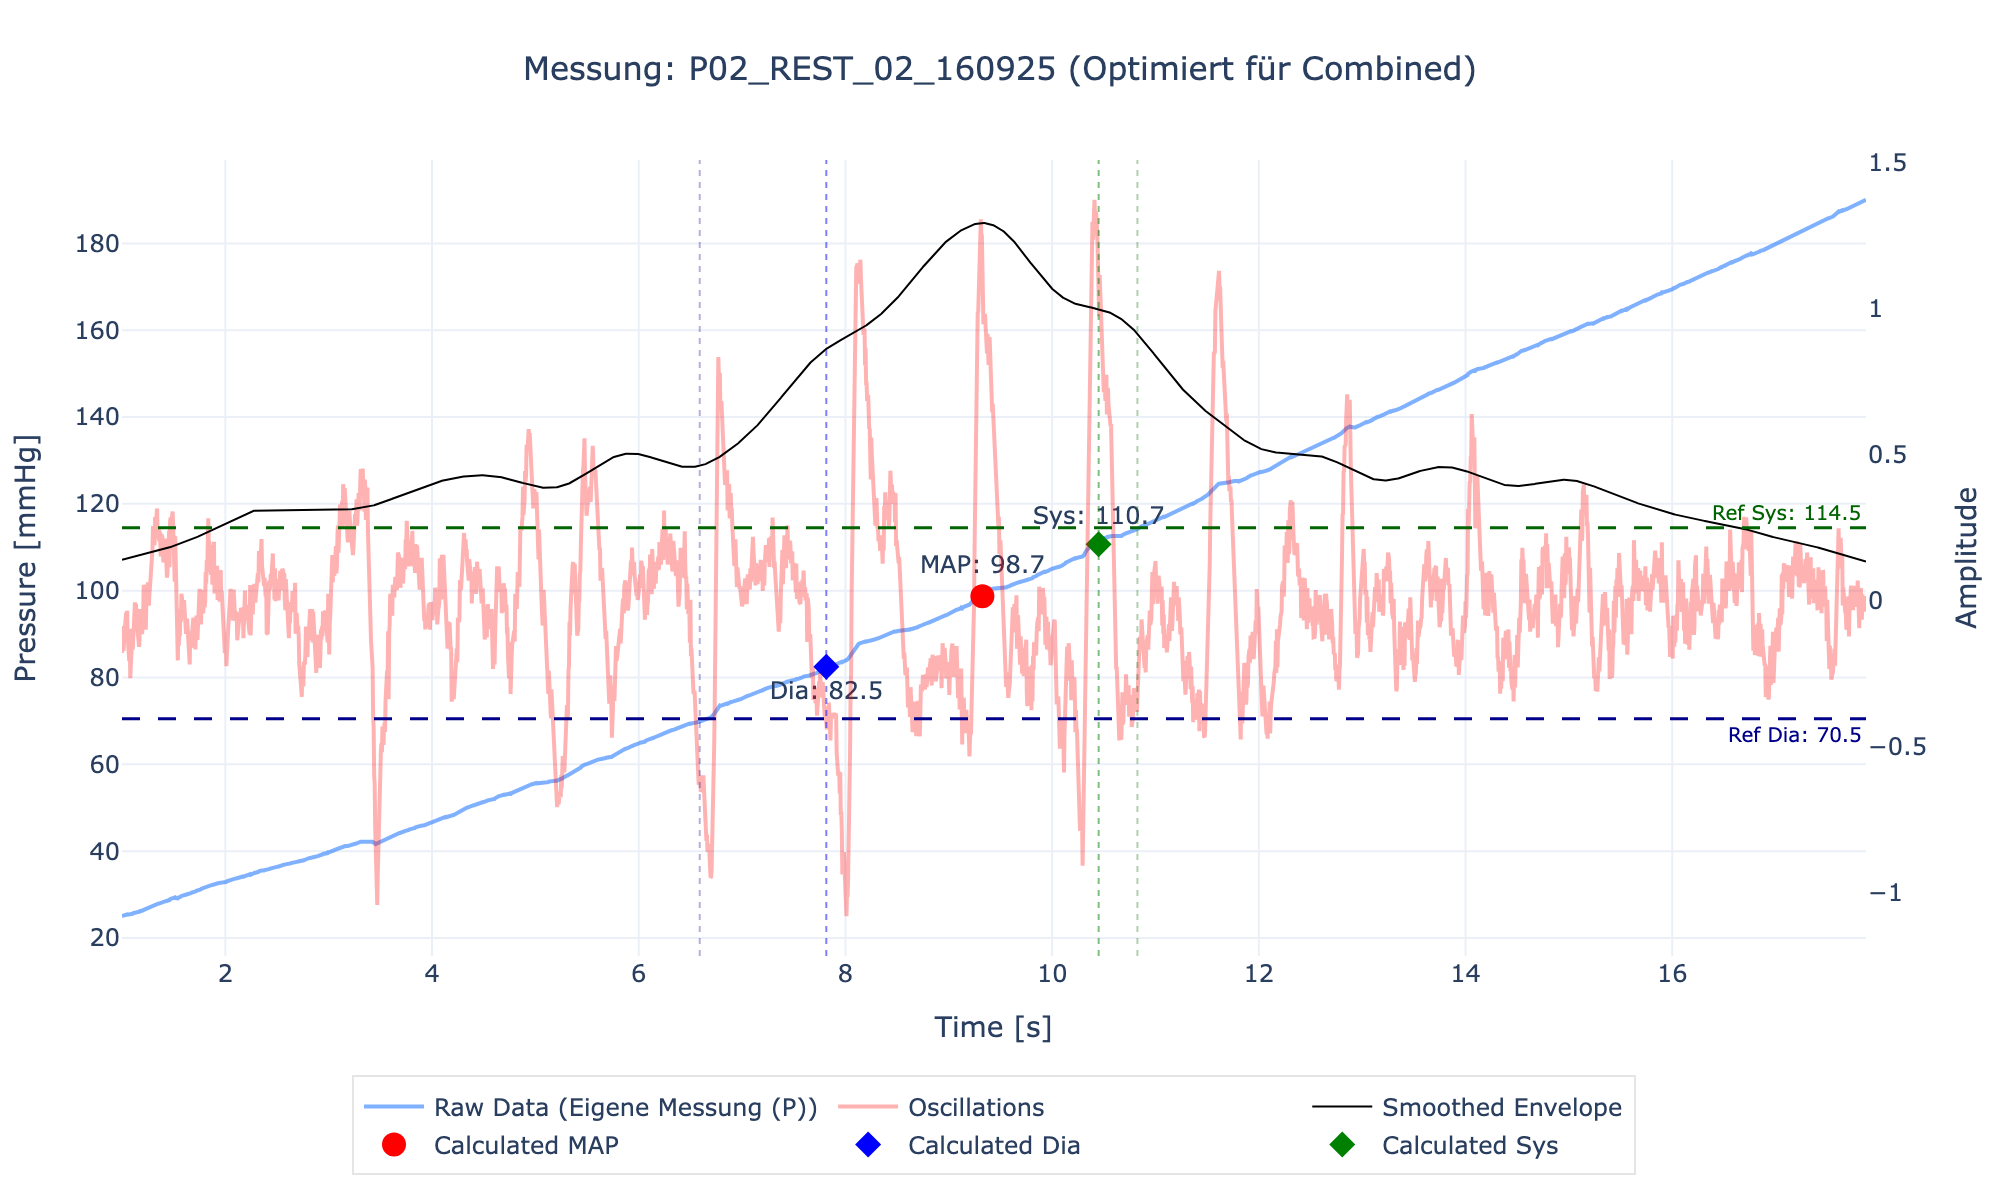
\includegraphics[width=\textwidth]{images/P02_REST_02_160925_combined.png}
        \caption{Optimiert für Beurer und NAIS (Kombiniert)}
    \end{subfigure} \\
    \begin{subfigure}[b]{0.48\textwidth}
        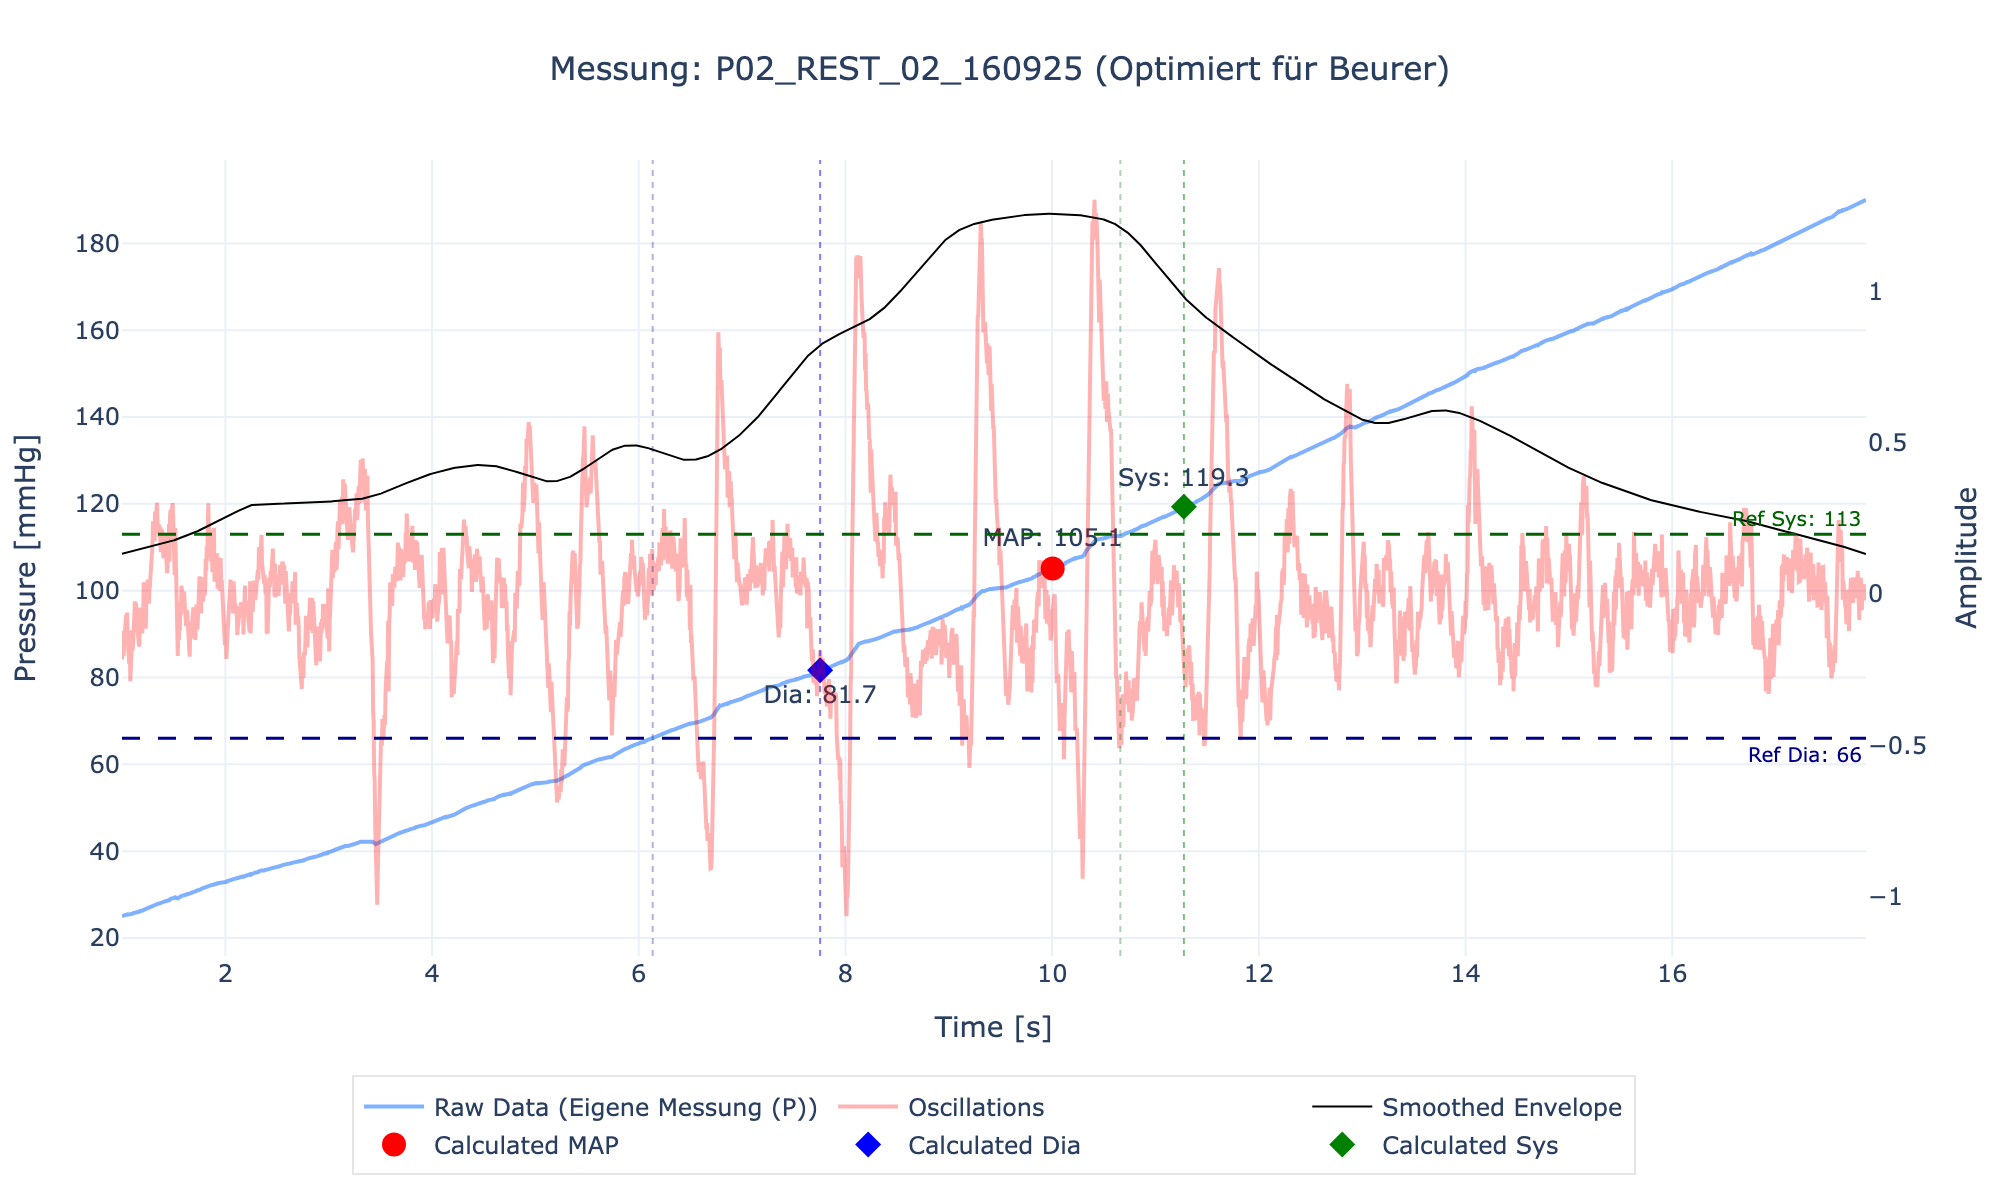
\includegraphics[width=\textwidth]{images/P02_REST_02_160925_beurer.png}
        \caption{Optimiert für Beurer}
    \end{subfigure}
    \hfill
    \begin{subfigure}[b]{0.48\textwidth}
        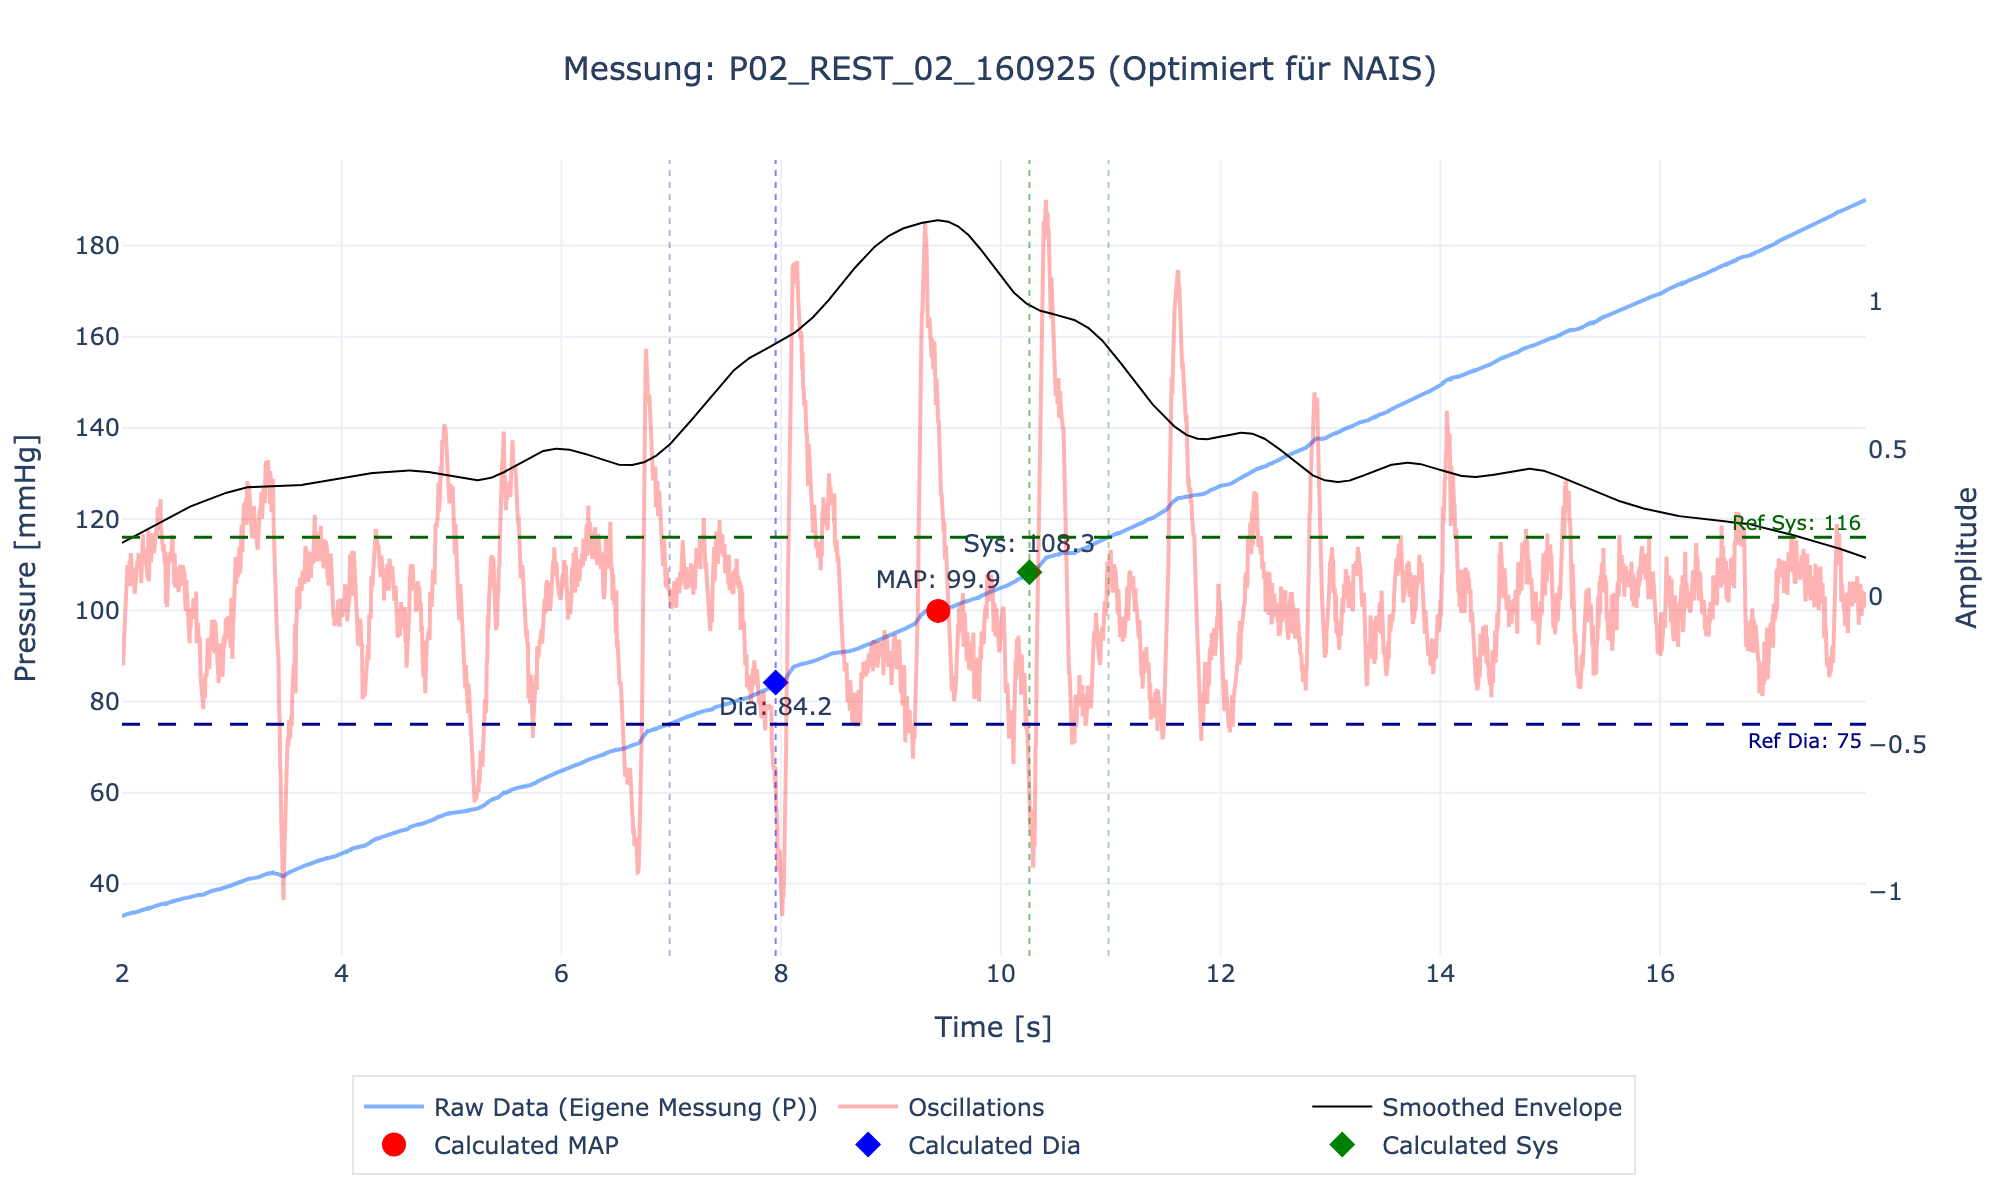
\includegraphics[width=\textwidth]{images/P02_REST_02_160925_nais.png}
        \caption{Optimiert für NAIS}
    \end{subfigure}
    \caption{Einzelauswertung der Messung P02\_REST\_02\_160925 mit verschiedenen Parametersätzen.}
\end{figure}
\newpage

\subsection*{Messung: P03\_ACTIV\_02\_160925}
\begin{figure}[H]
    \centering
    \begin{subfigure}[b]{0.8\textwidth}
        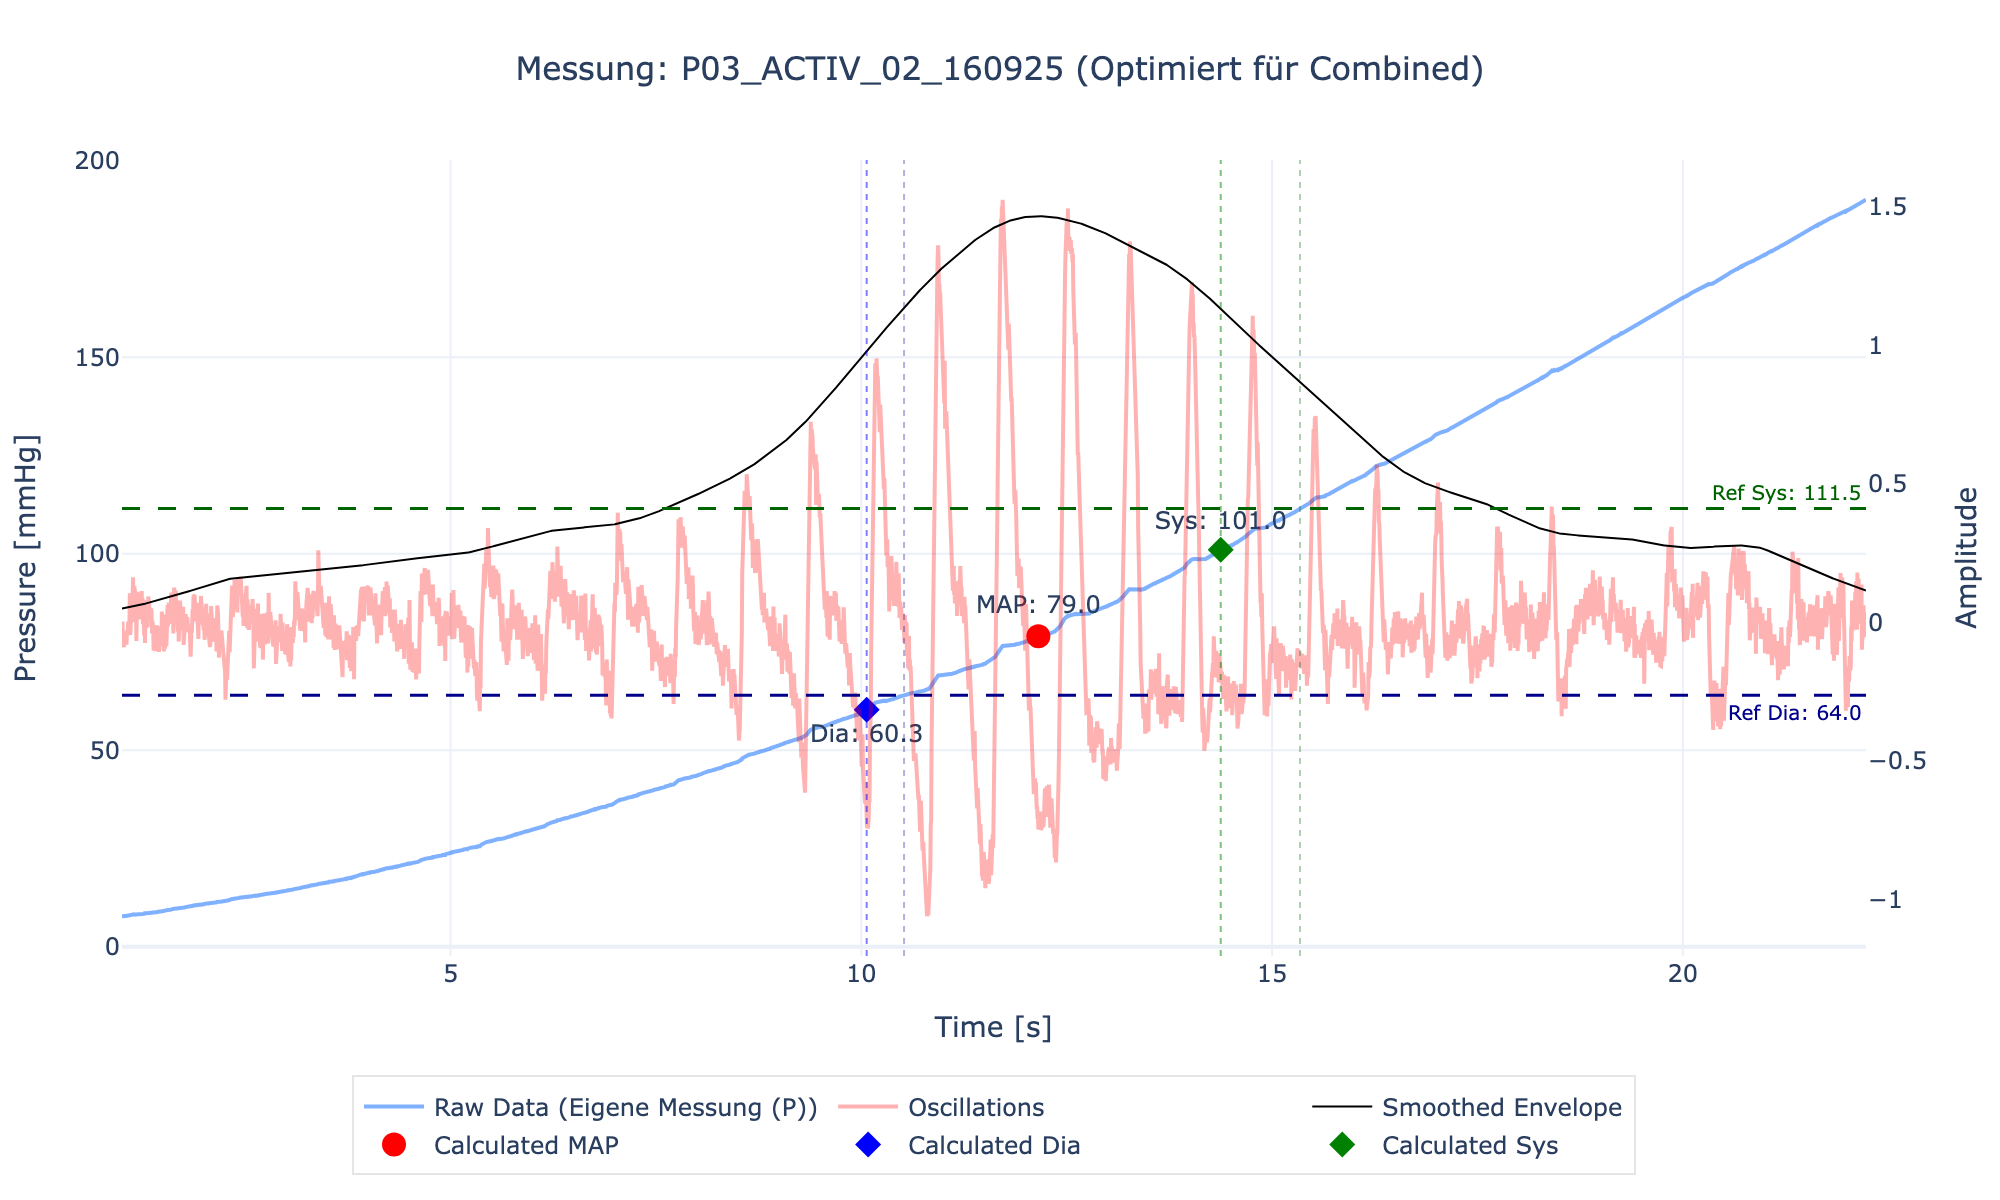
\includegraphics[width=\textwidth]{images/P03_ACTIV_02_160925_combined.png}
        \caption{Optimiert für Beurer und NAIS (Kombiniert)}
    \end{subfigure} \\
    \begin{subfigure}[b]{0.48\textwidth}
        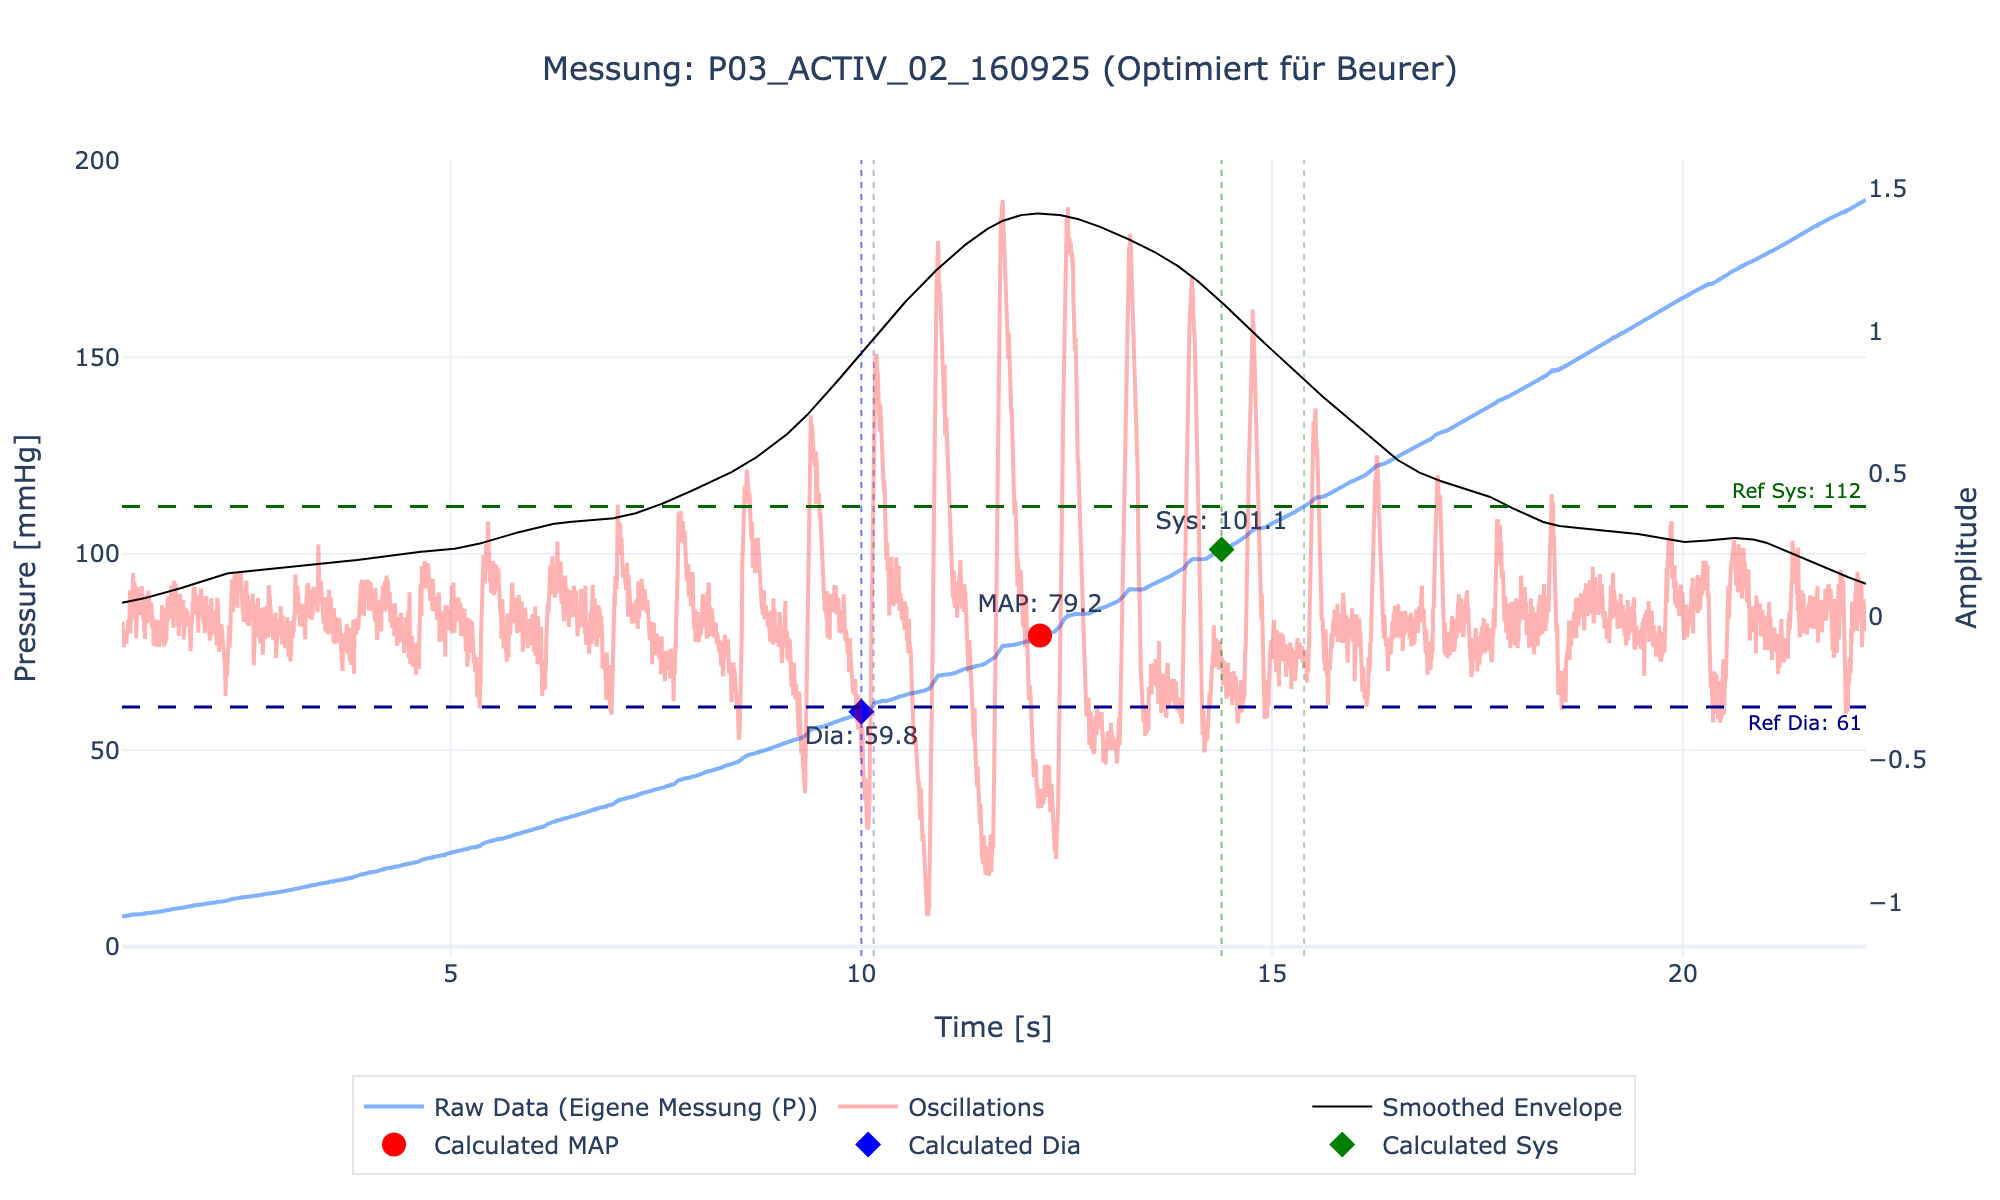
\includegraphics[width=\textwidth]{images/P03_ACTIV_02_160925_beurer.png}
        \caption{Optimiert für Beurer}
    \end{subfigure}
    \hfill
    \begin{subfigure}[b]{0.48\textwidth}
        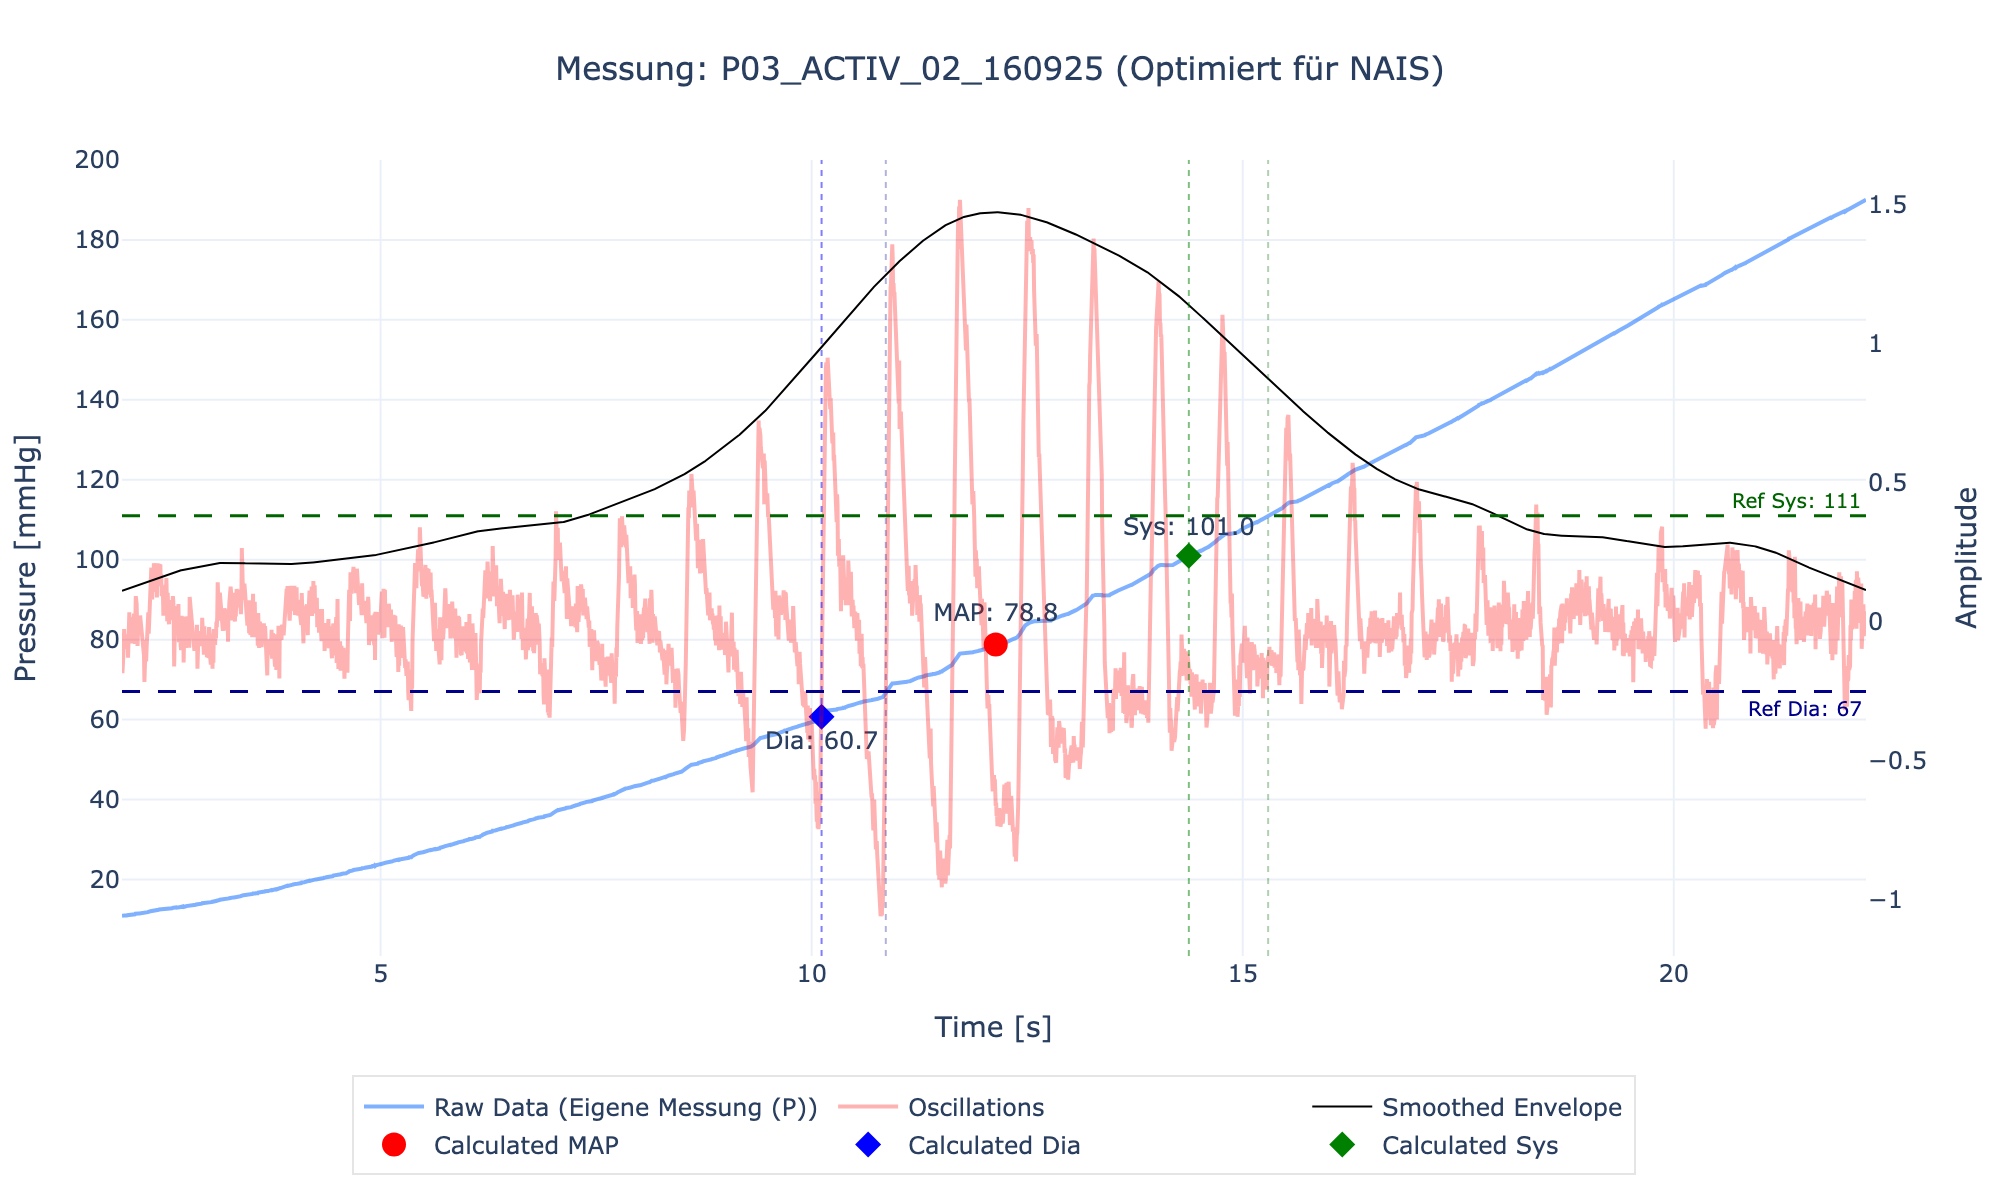
\includegraphics[width=\textwidth]{images/P03_ACTIV_02_160925_nais.png}
        \caption{Optimiert für NAIS}
    \end{subfigure}
    \caption{Einzelauswertung der Messung P03\_ACTIV\_02\_160925 mit verschiedenen Parametersätzen.}
\end{figure}
\newpage

\subsection*{Messung: P03\_REST\_01\_100825}
\begin{figure}[H]
    \centering
    \begin{subfigure}[b]{0.8\textwidth}
        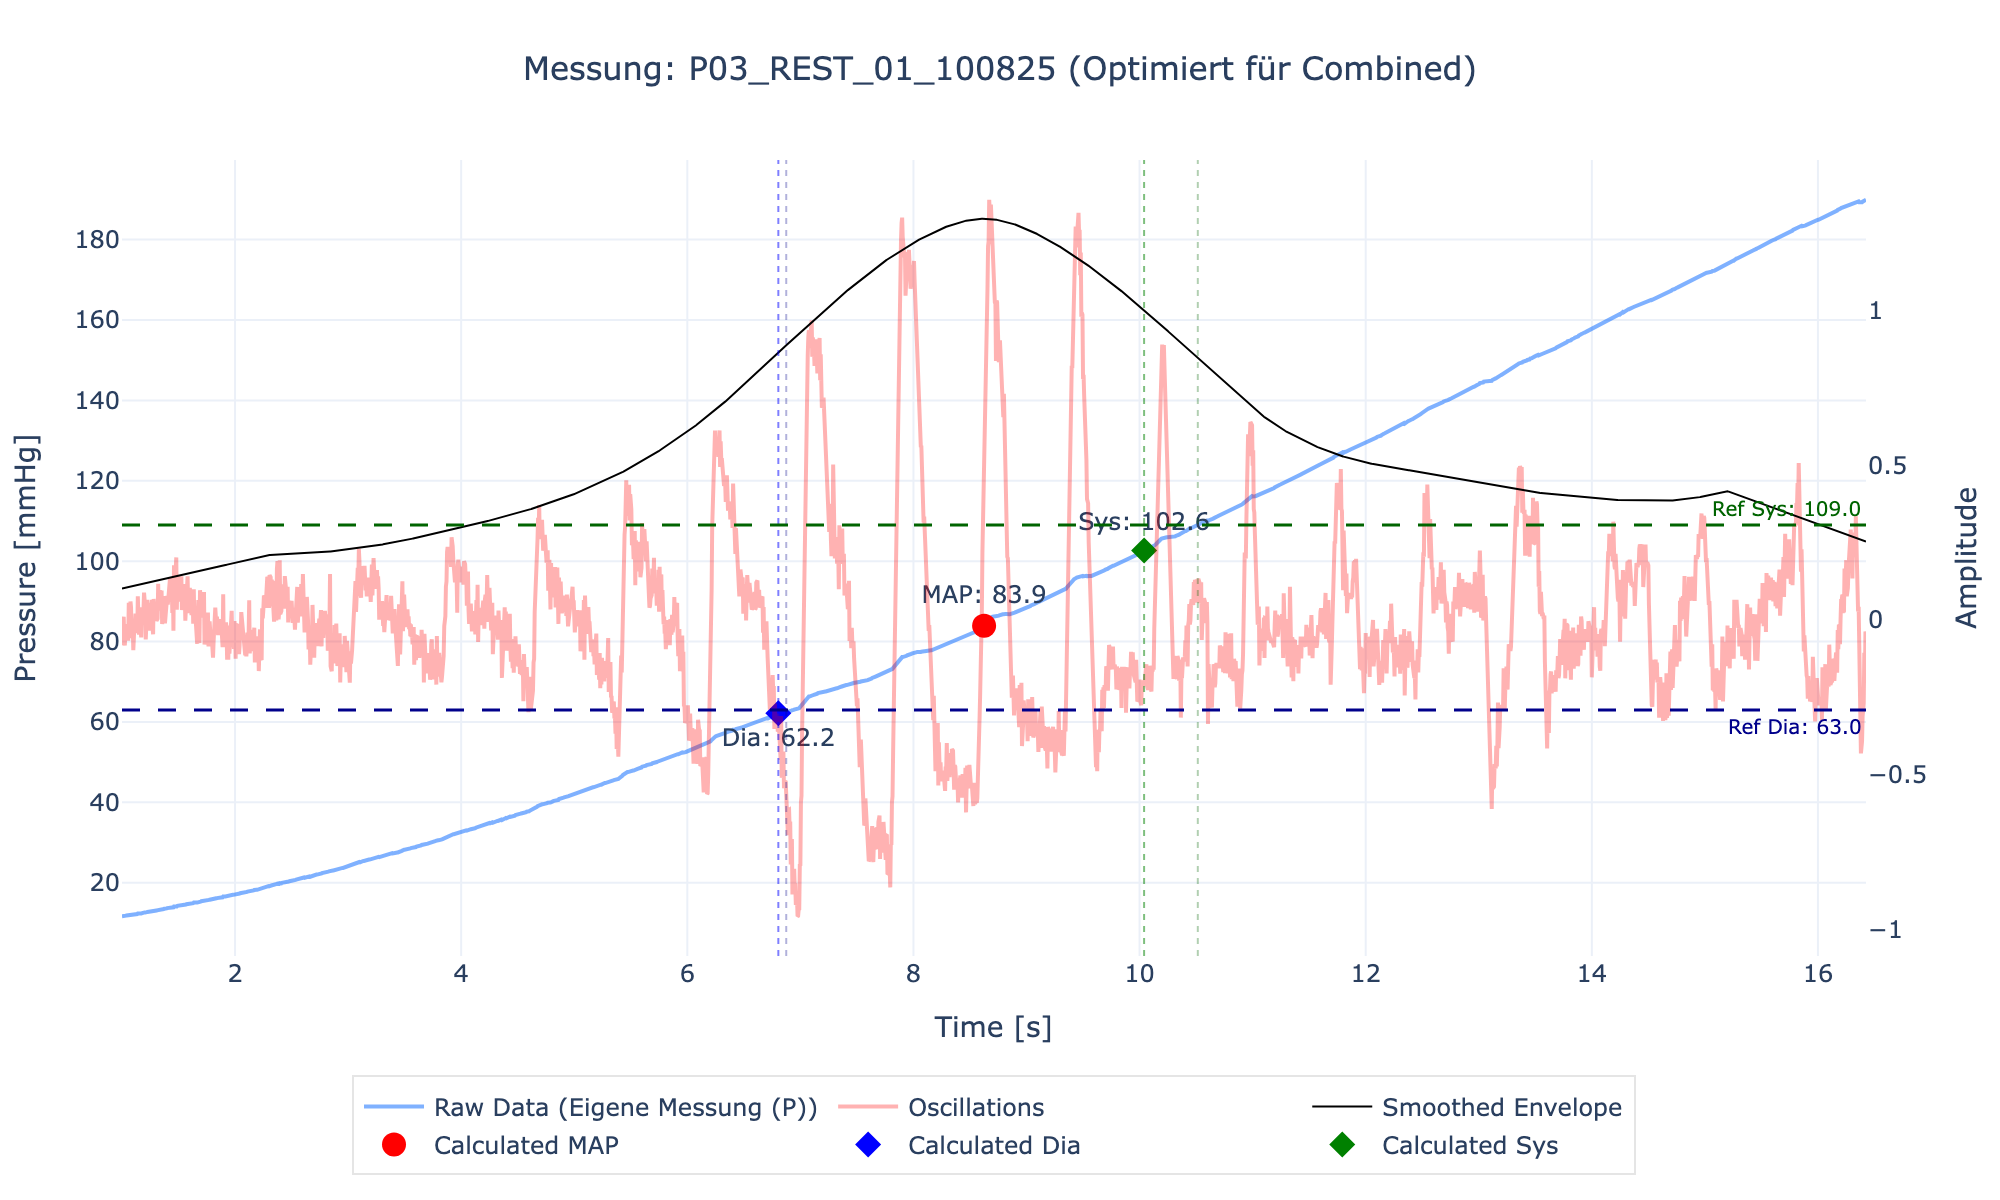
\includegraphics[width=\textwidth]{images/P03_REST_01_100825_combined.png}
        \caption{Optimiert für Beurer und NAIS (Kombiniert)}
    \end{subfigure} \\
    \begin{subfigure}[b]{0.48\textwidth}
        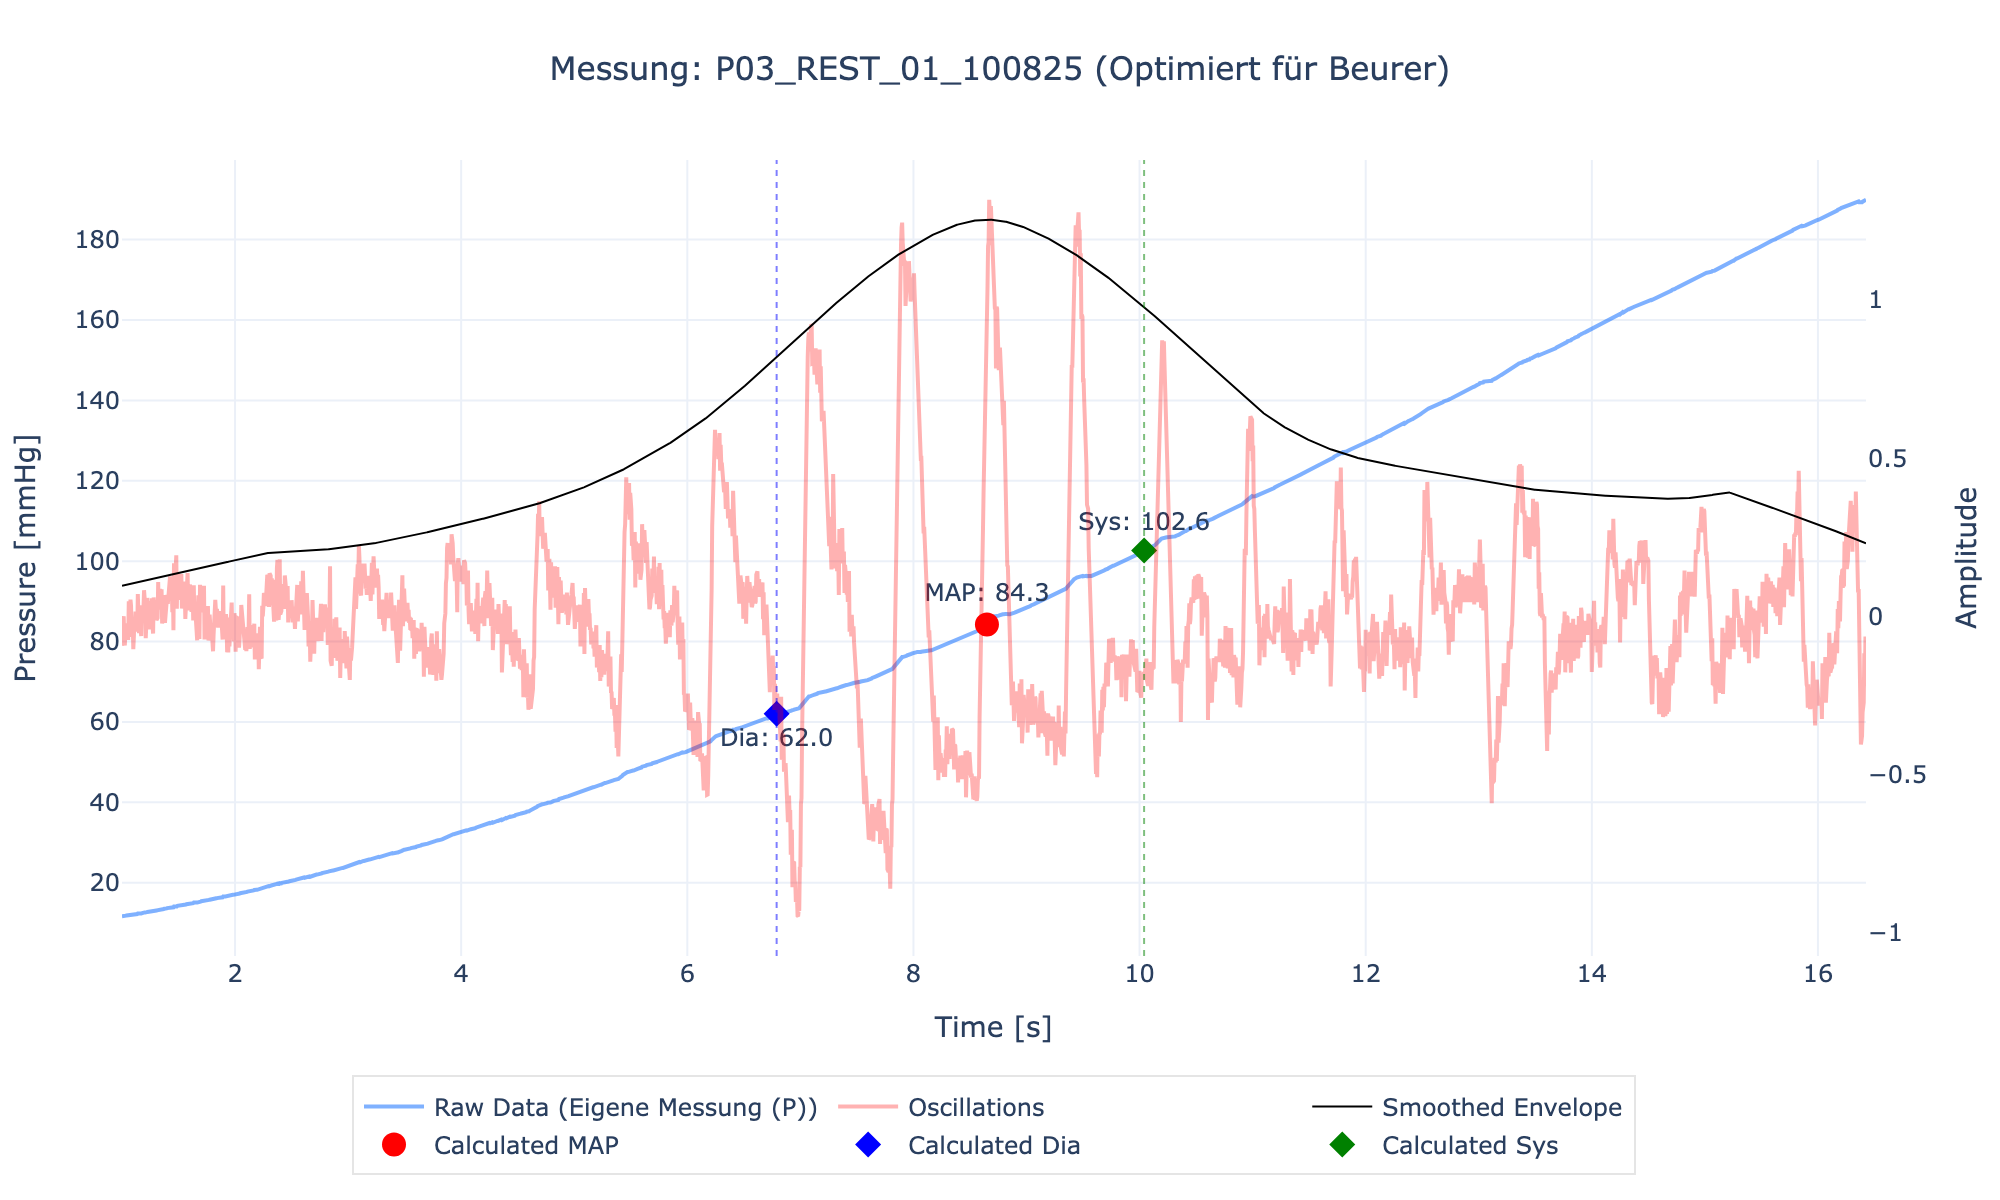
\includegraphics[width=\textwidth]{images/P03_REST_01_100825_beurer.png}
        \caption{Optimiert für Beurer}
    \end{subfigure}
    \hfill
    \begin{subfigure}[b]{0.48\textwidth}
        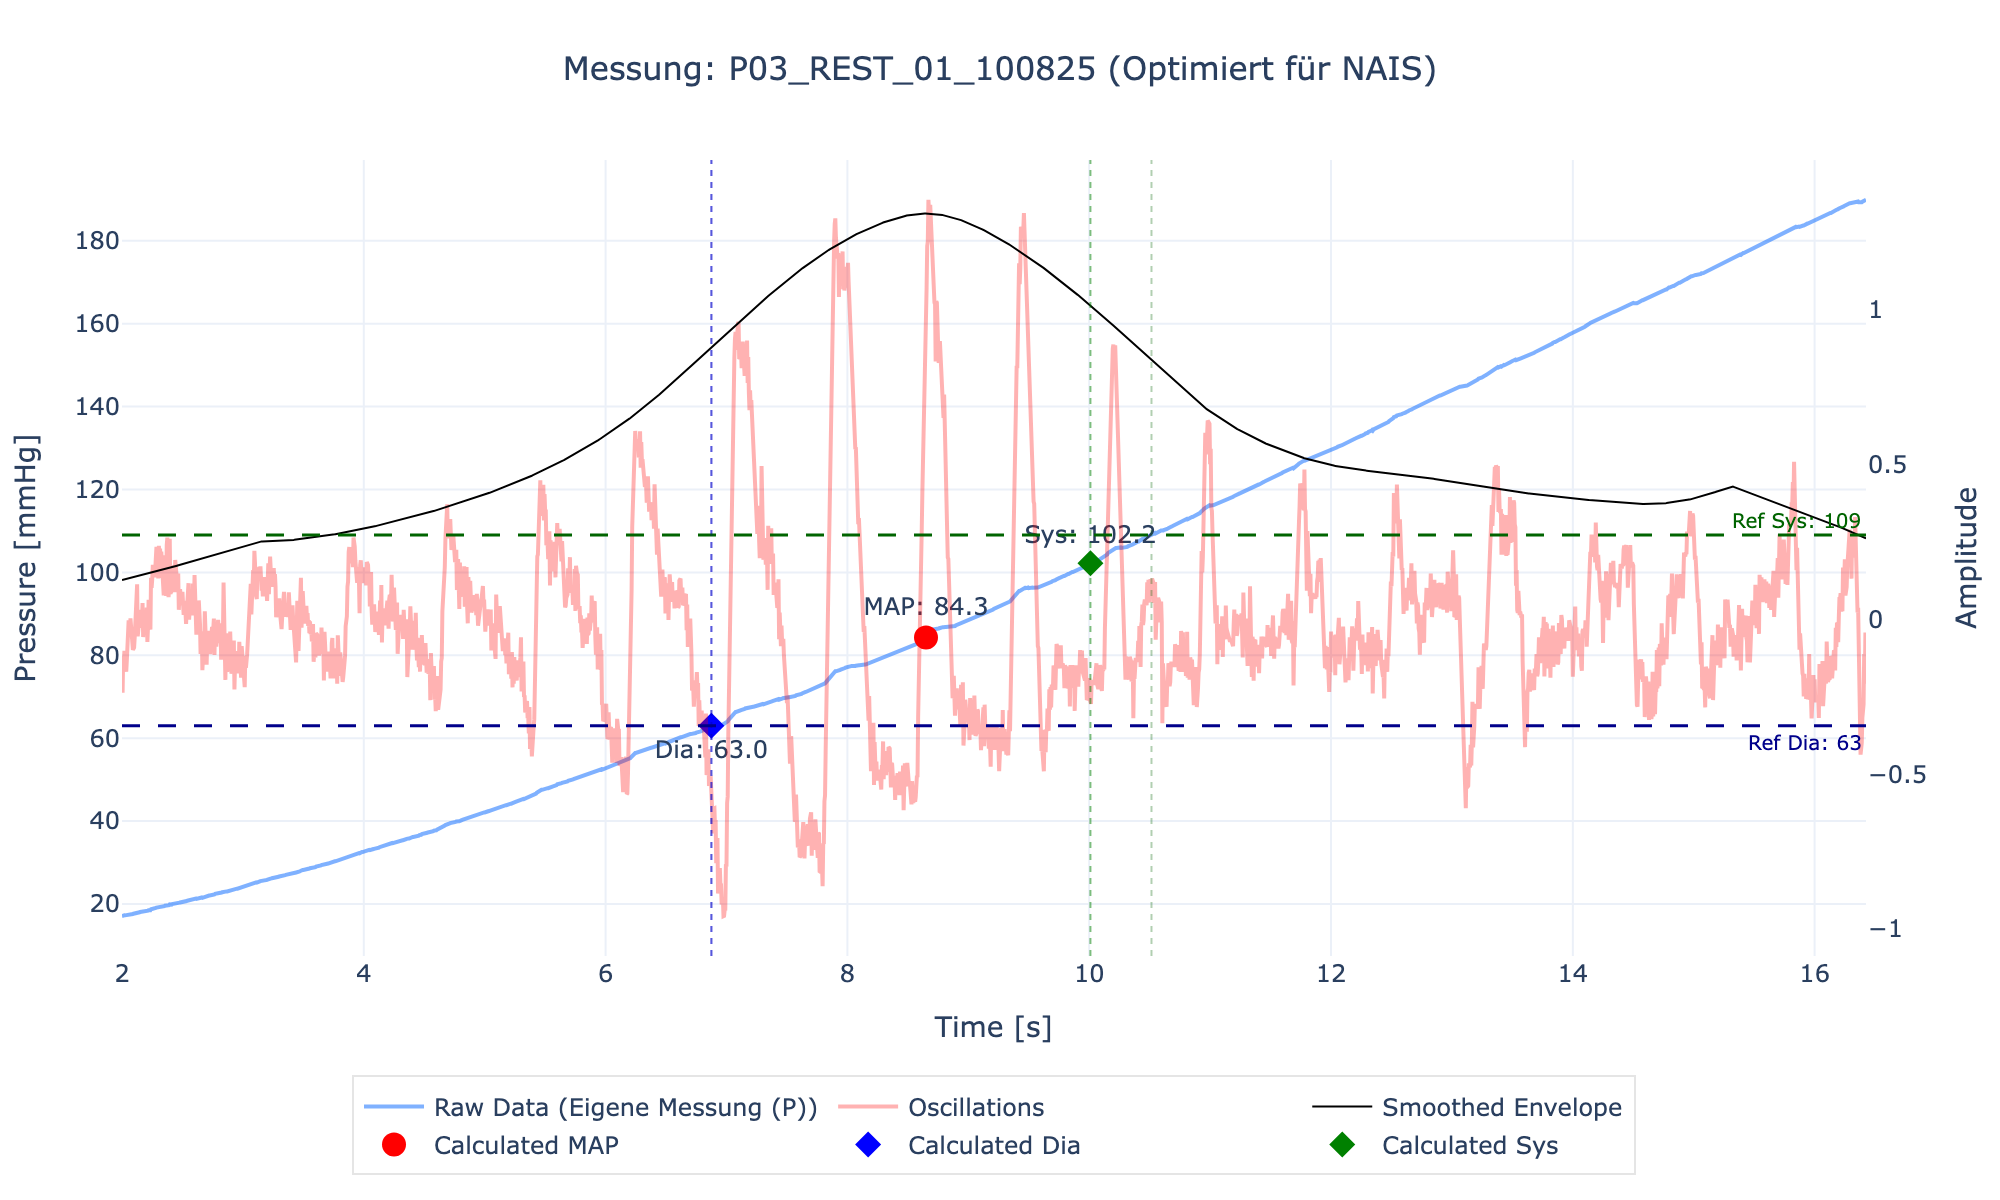
\includegraphics[width=\textwidth]{images/P03_REST_01_100825_nais.png}
        \caption{Optimiert für NAIS}
    \end{subfigure}
    \caption{Einzelauswertung der Messung P03\_REST\_01\_100825 mit verschiedenen Parametersätzen.}
\end{figure}
\newpage

\subsection*{Messung: P03\_REST\_02\_160925}
\begin{figure}[H]
    \centering
    \begin{subfigure}[b]{0.8\textwidth}
        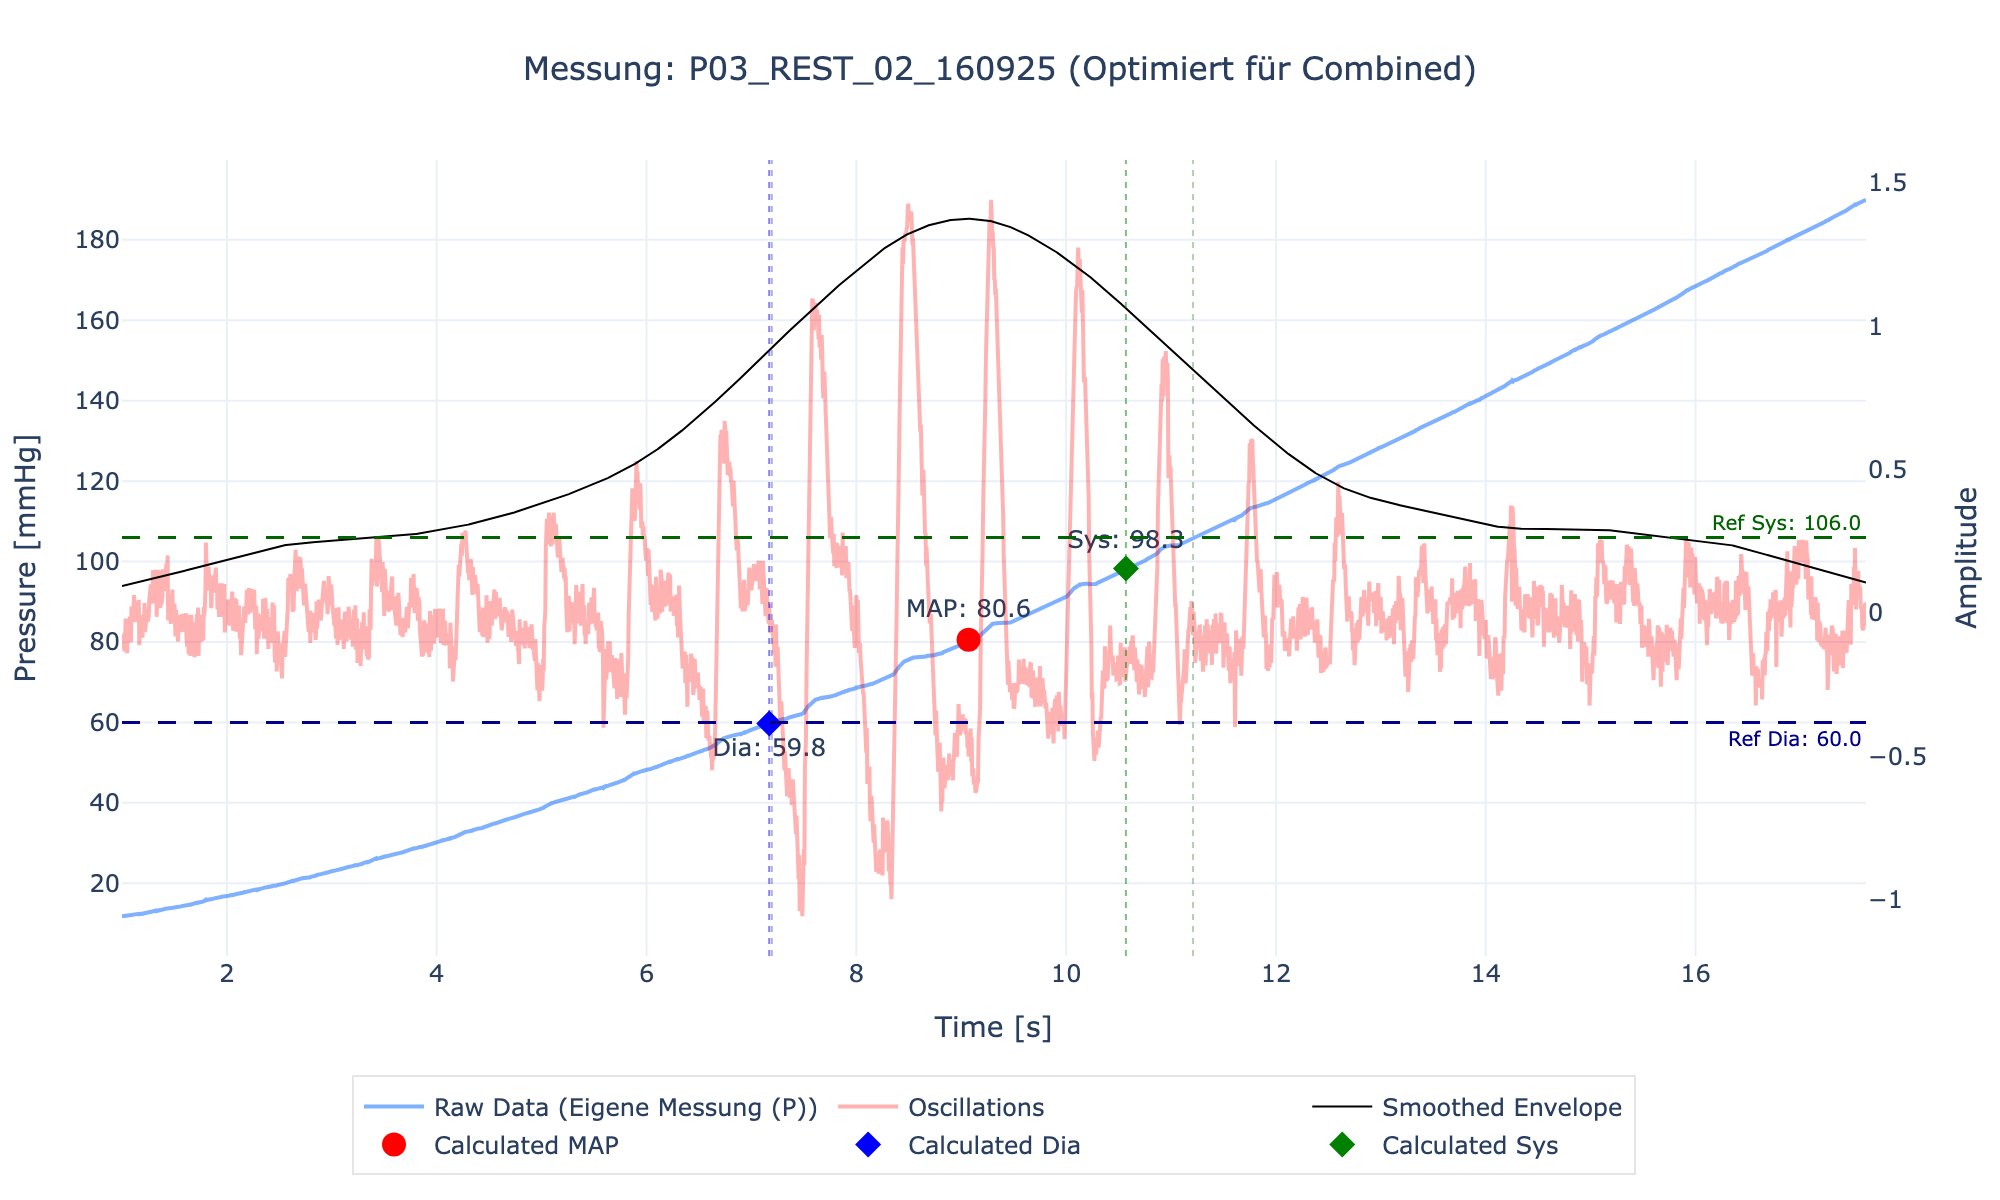
\includegraphics[width=\textwidth]{images/P03_REST_02_160925_combined.png}
        \caption{Optimiert für Beurer und NAIS (Kombiniert)}
    \end{subfigure} \\
    \begin{subfigure}[b]{0.48\textwidth}
        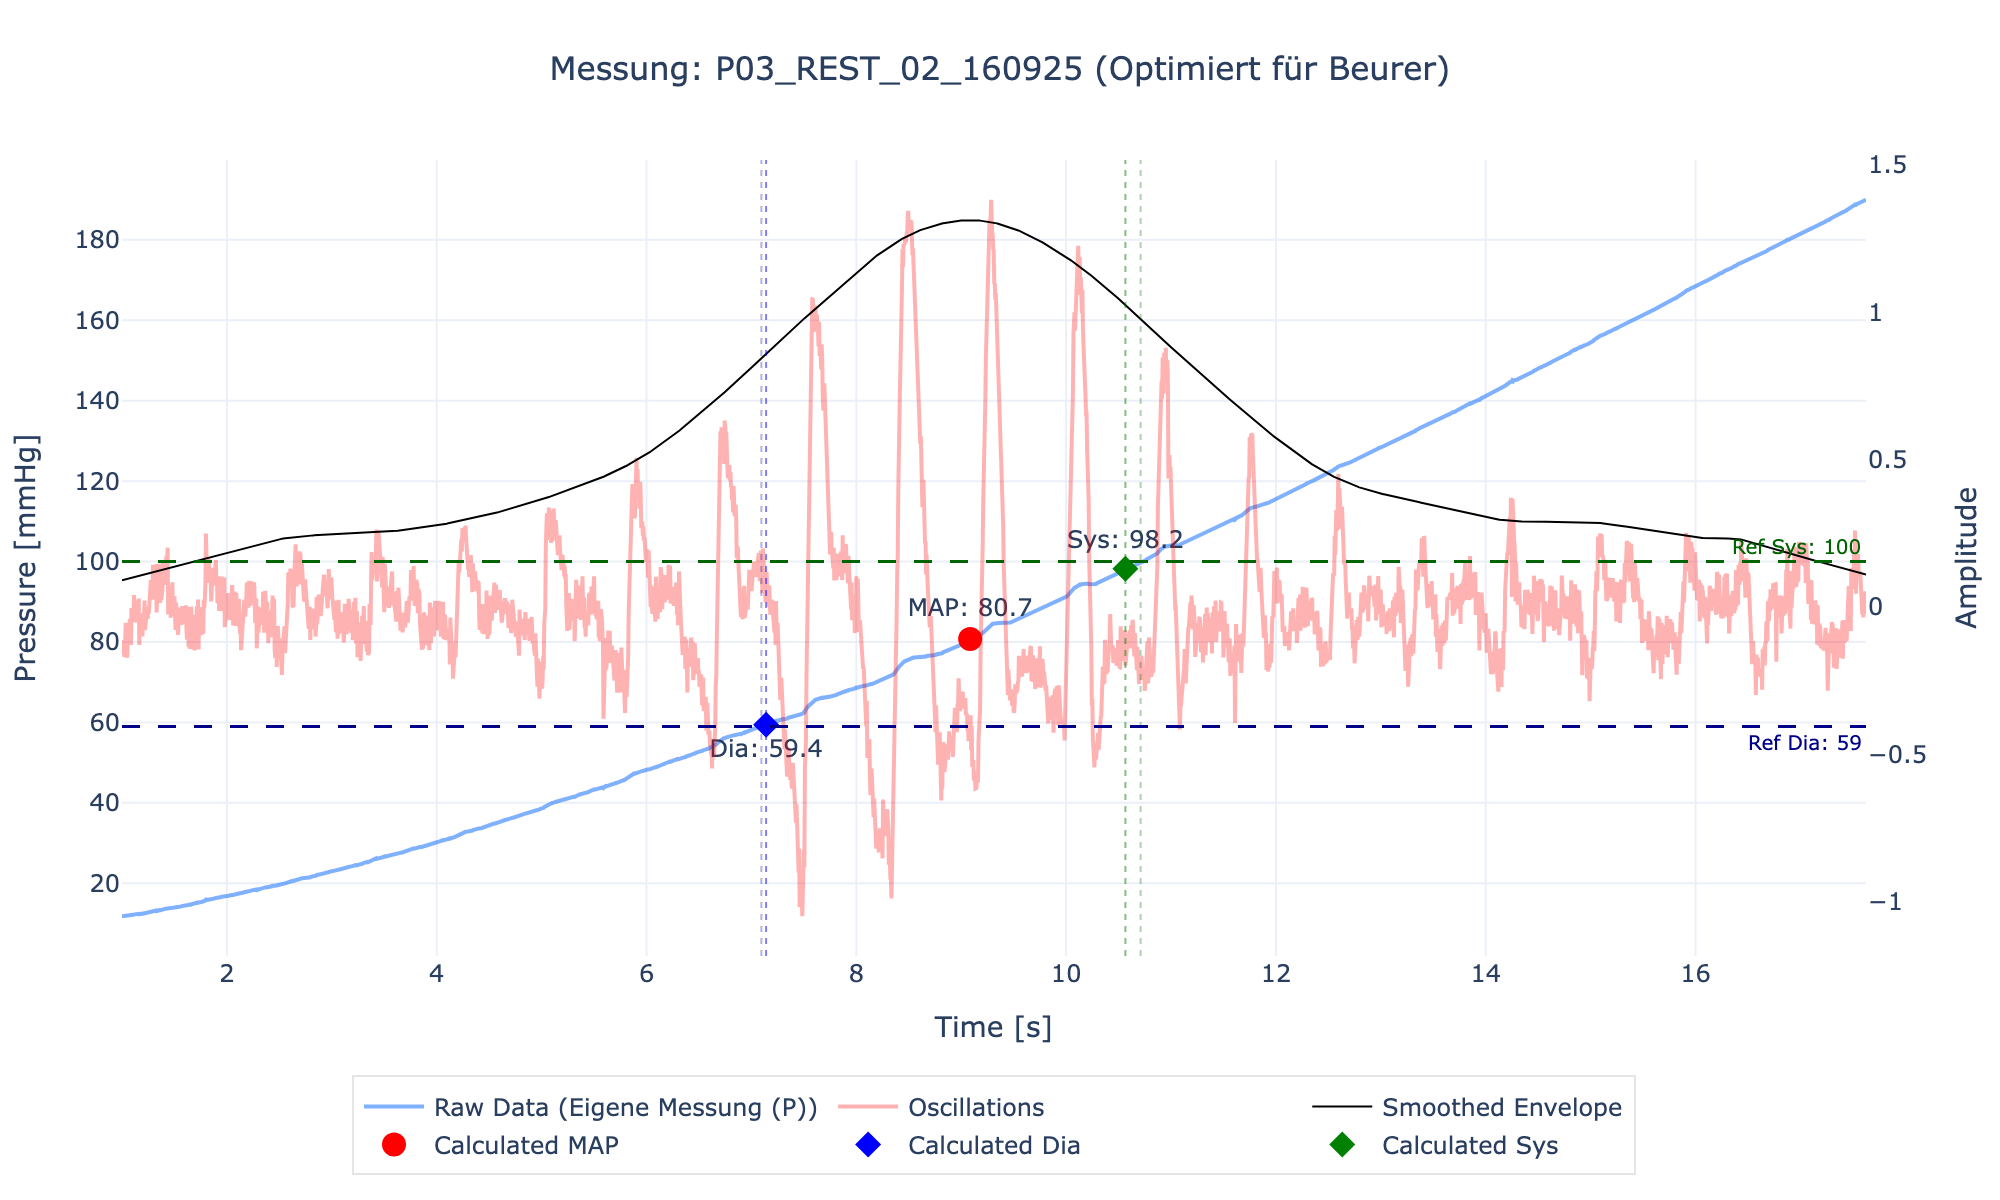
\includegraphics[width=\textwidth]{images/P03_REST_02_160925_beurer.png}
        \caption{Optimiert für Beurer}
    \end{subfigure}
    \hfill
    \begin{subfigure}[b]{0.48\textwidth}
        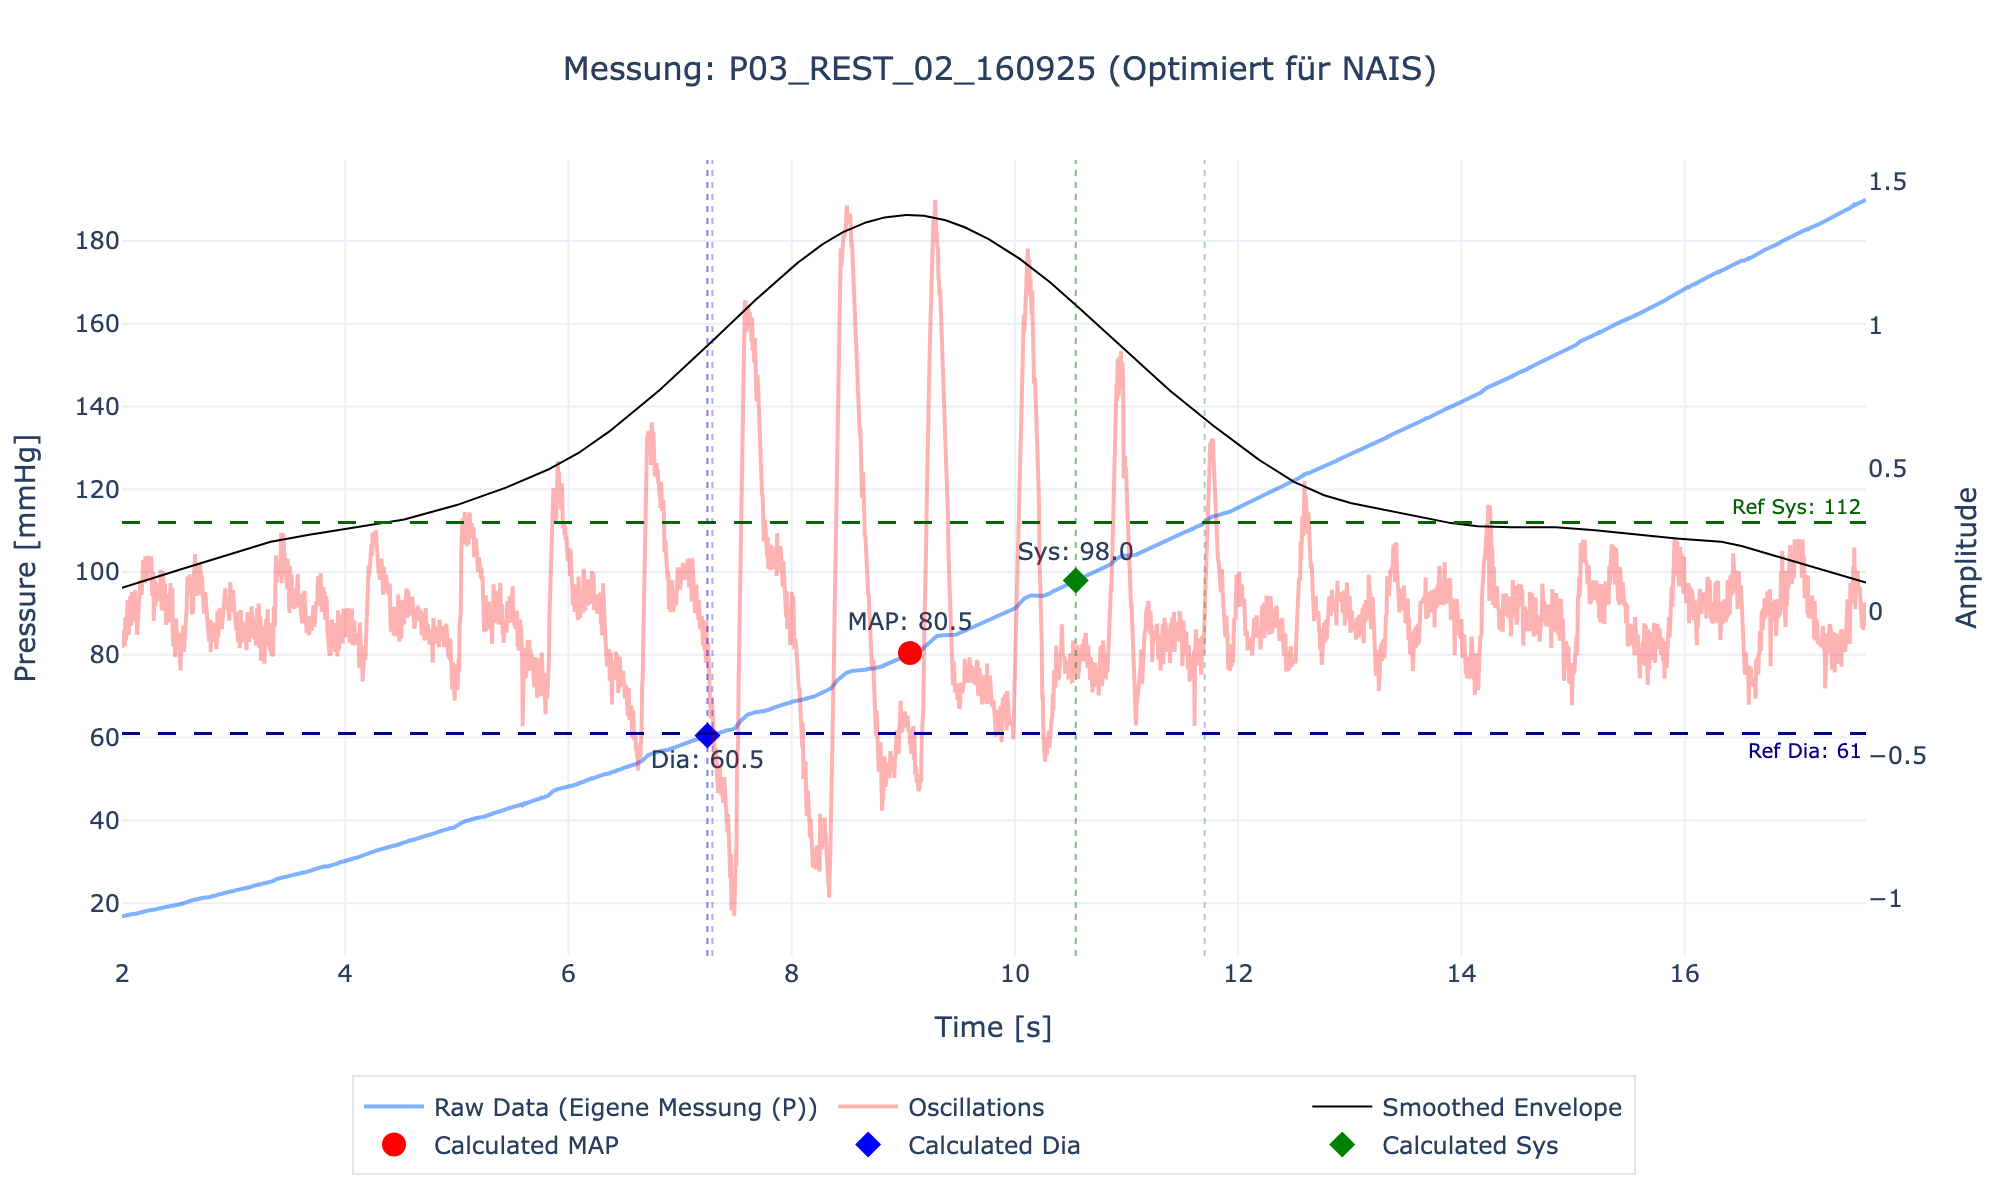
\includegraphics[width=\textwidth]{images/P03_REST_02_160925_nais.png}
        \caption{Optimiert für NAIS}
    \end{subfigure}
    \caption{Einzelauswertung der Messung P03\_REST\_02\_160925 mit verschiedenen Parametersätzen.}
\end{figure}
\newpage

\subsection*{Messung: P04\_ACTIV\_01\_160925}
\begin{figure}[H]
    \centering
    \begin{subfigure}[b]{0.8\textwidth}
        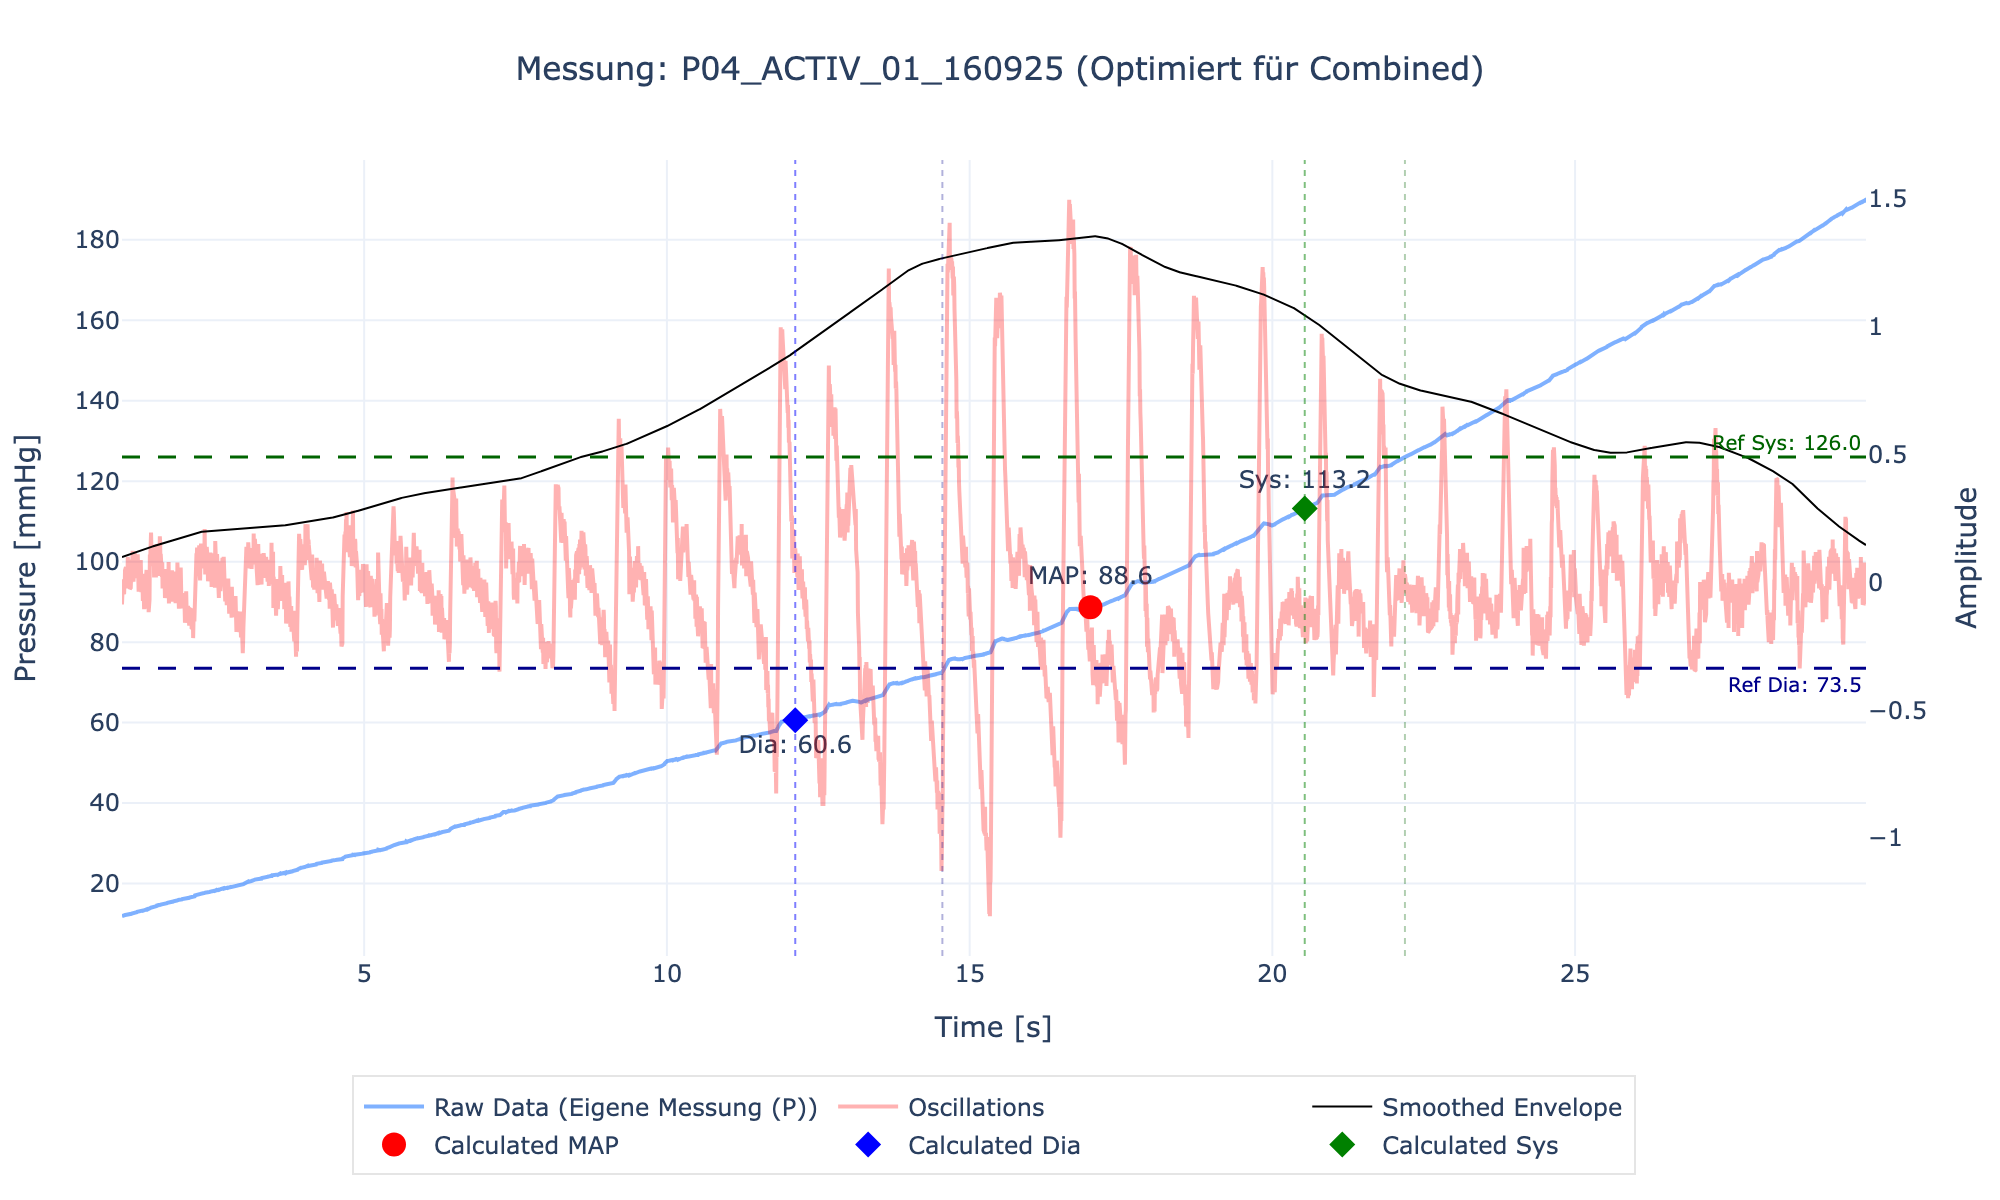
\includegraphics[width=\textwidth]{images/P04_ACTIV_01_160925_combined.png}
        \caption{Optimiert für Beurer und NAIS (Kombiniert)}
    \end{subfigure} \\
    \begin{subfigure}[b]{0.48\textwidth}
        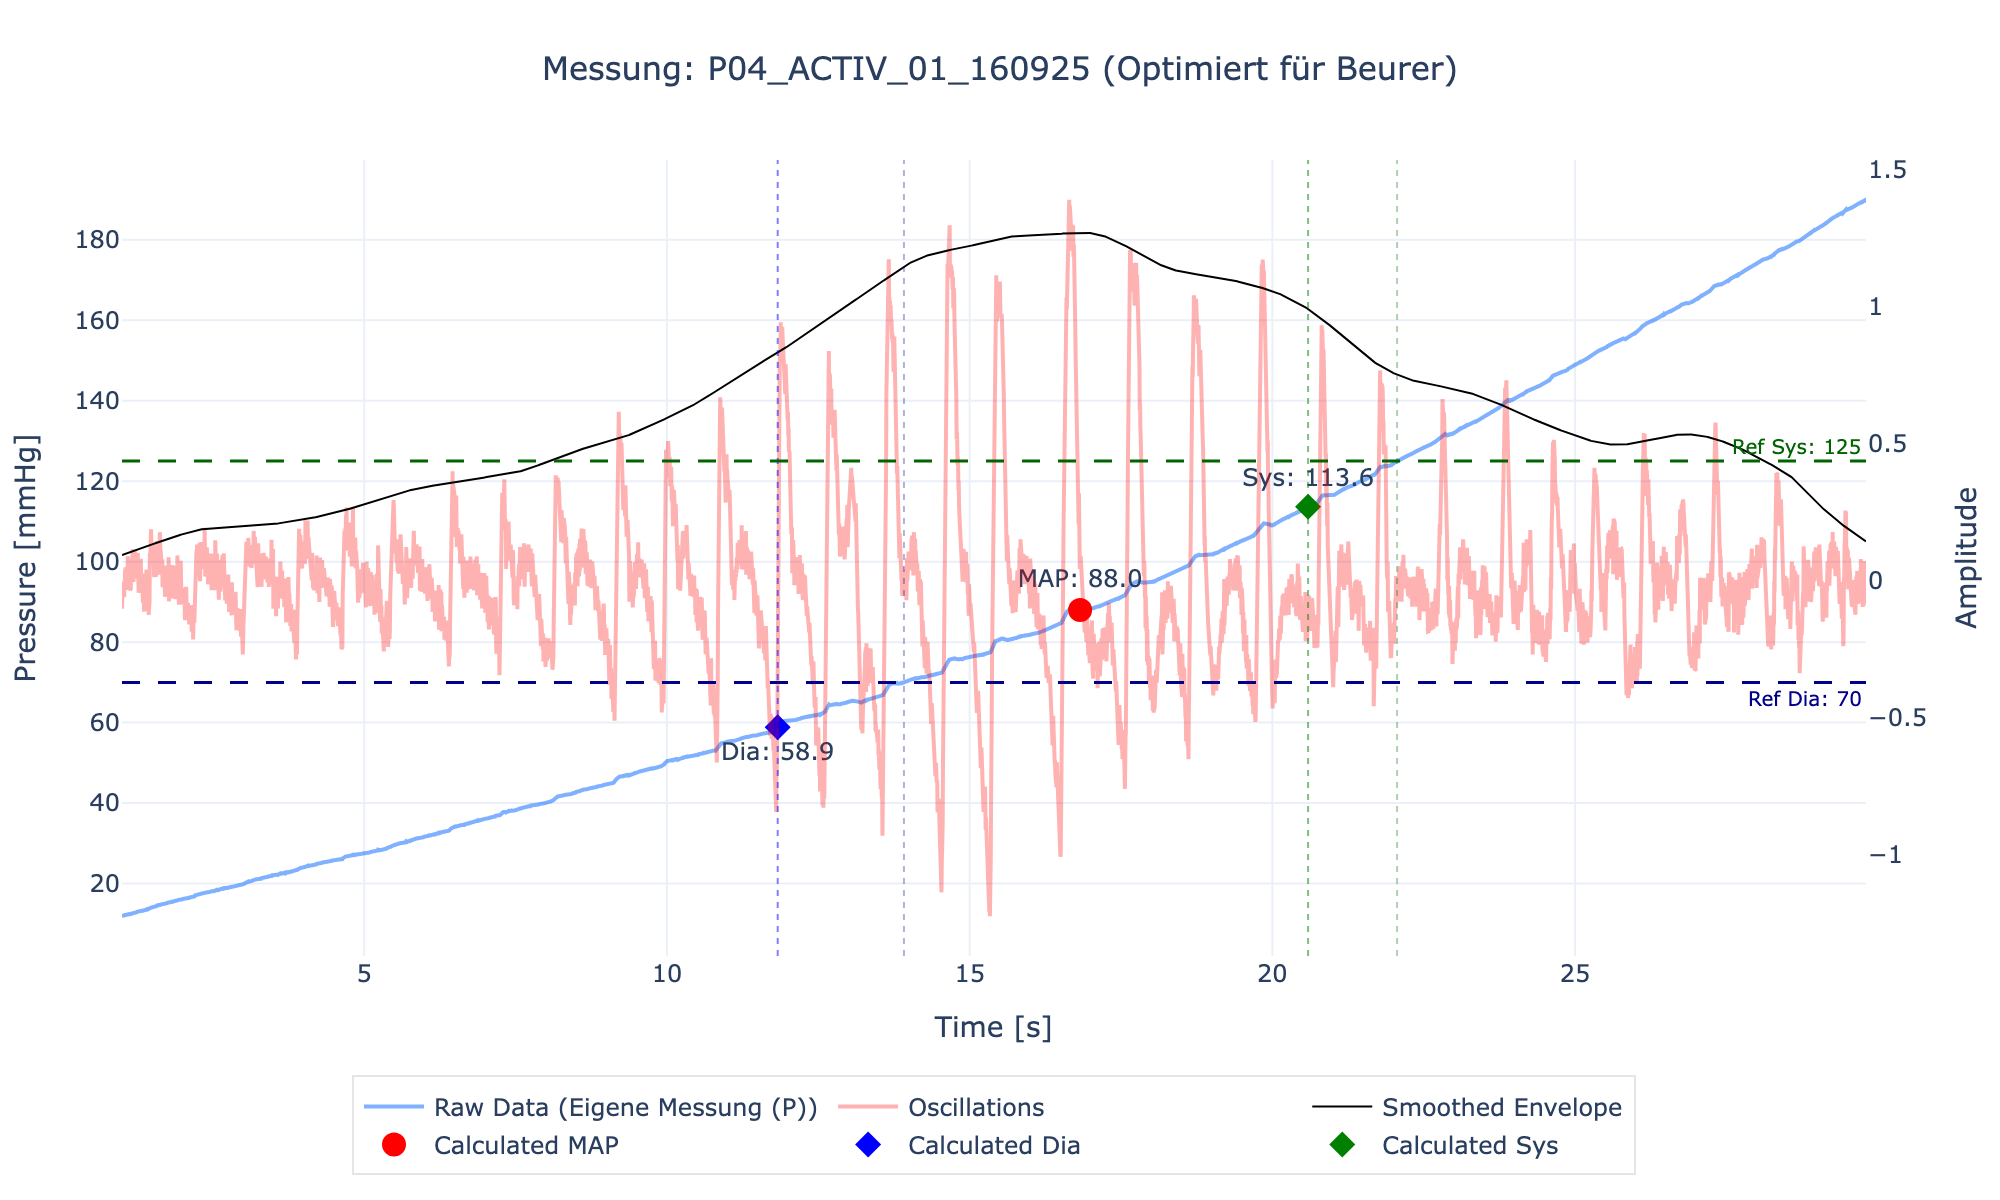
\includegraphics[width=\textwidth]{images/P04_ACTIV_01_160925_beurer.png}
        \caption{Optimiert für Beurer}
    \end{subfigure}
    \hfill
    \begin{subfigure}[b]{0.48\textwidth}
        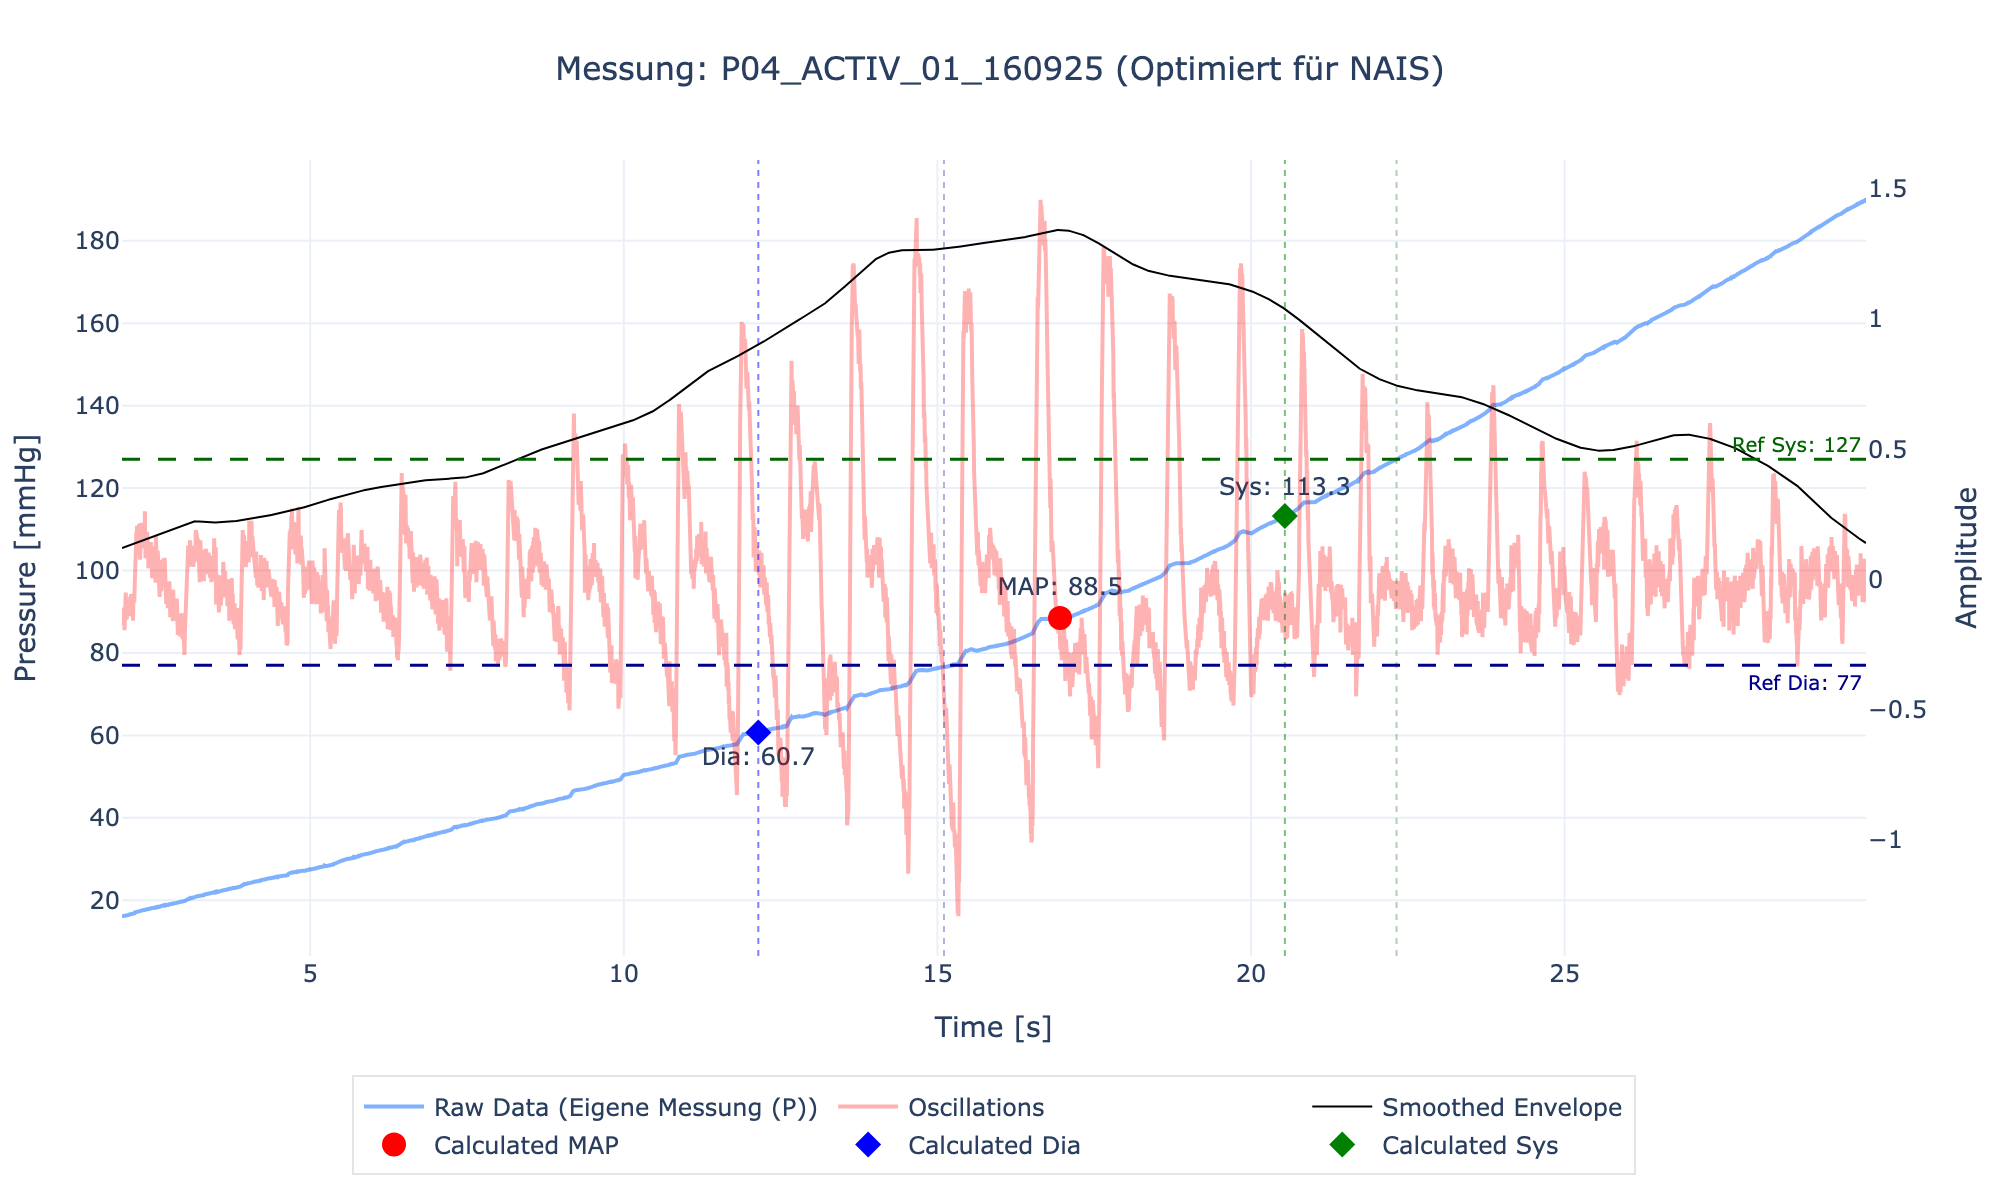
\includegraphics[width=\textwidth]{images/P04_ACTIV_01_160925_nais.png}
        \caption{Optimiert für NAIS}
    \end{subfigure}
    \caption{Einzelauswertung der Messung P04\_ACTIV\_01\_160925 mit verschiedenen Parametersätzen.}
\end{figure}
\newpage

\subsection*{Messung: P04\_REST\_01\_160925}
\begin{figure}[H]
    \centering
    \begin{subfigure}[b]{0.8\textwidth}
        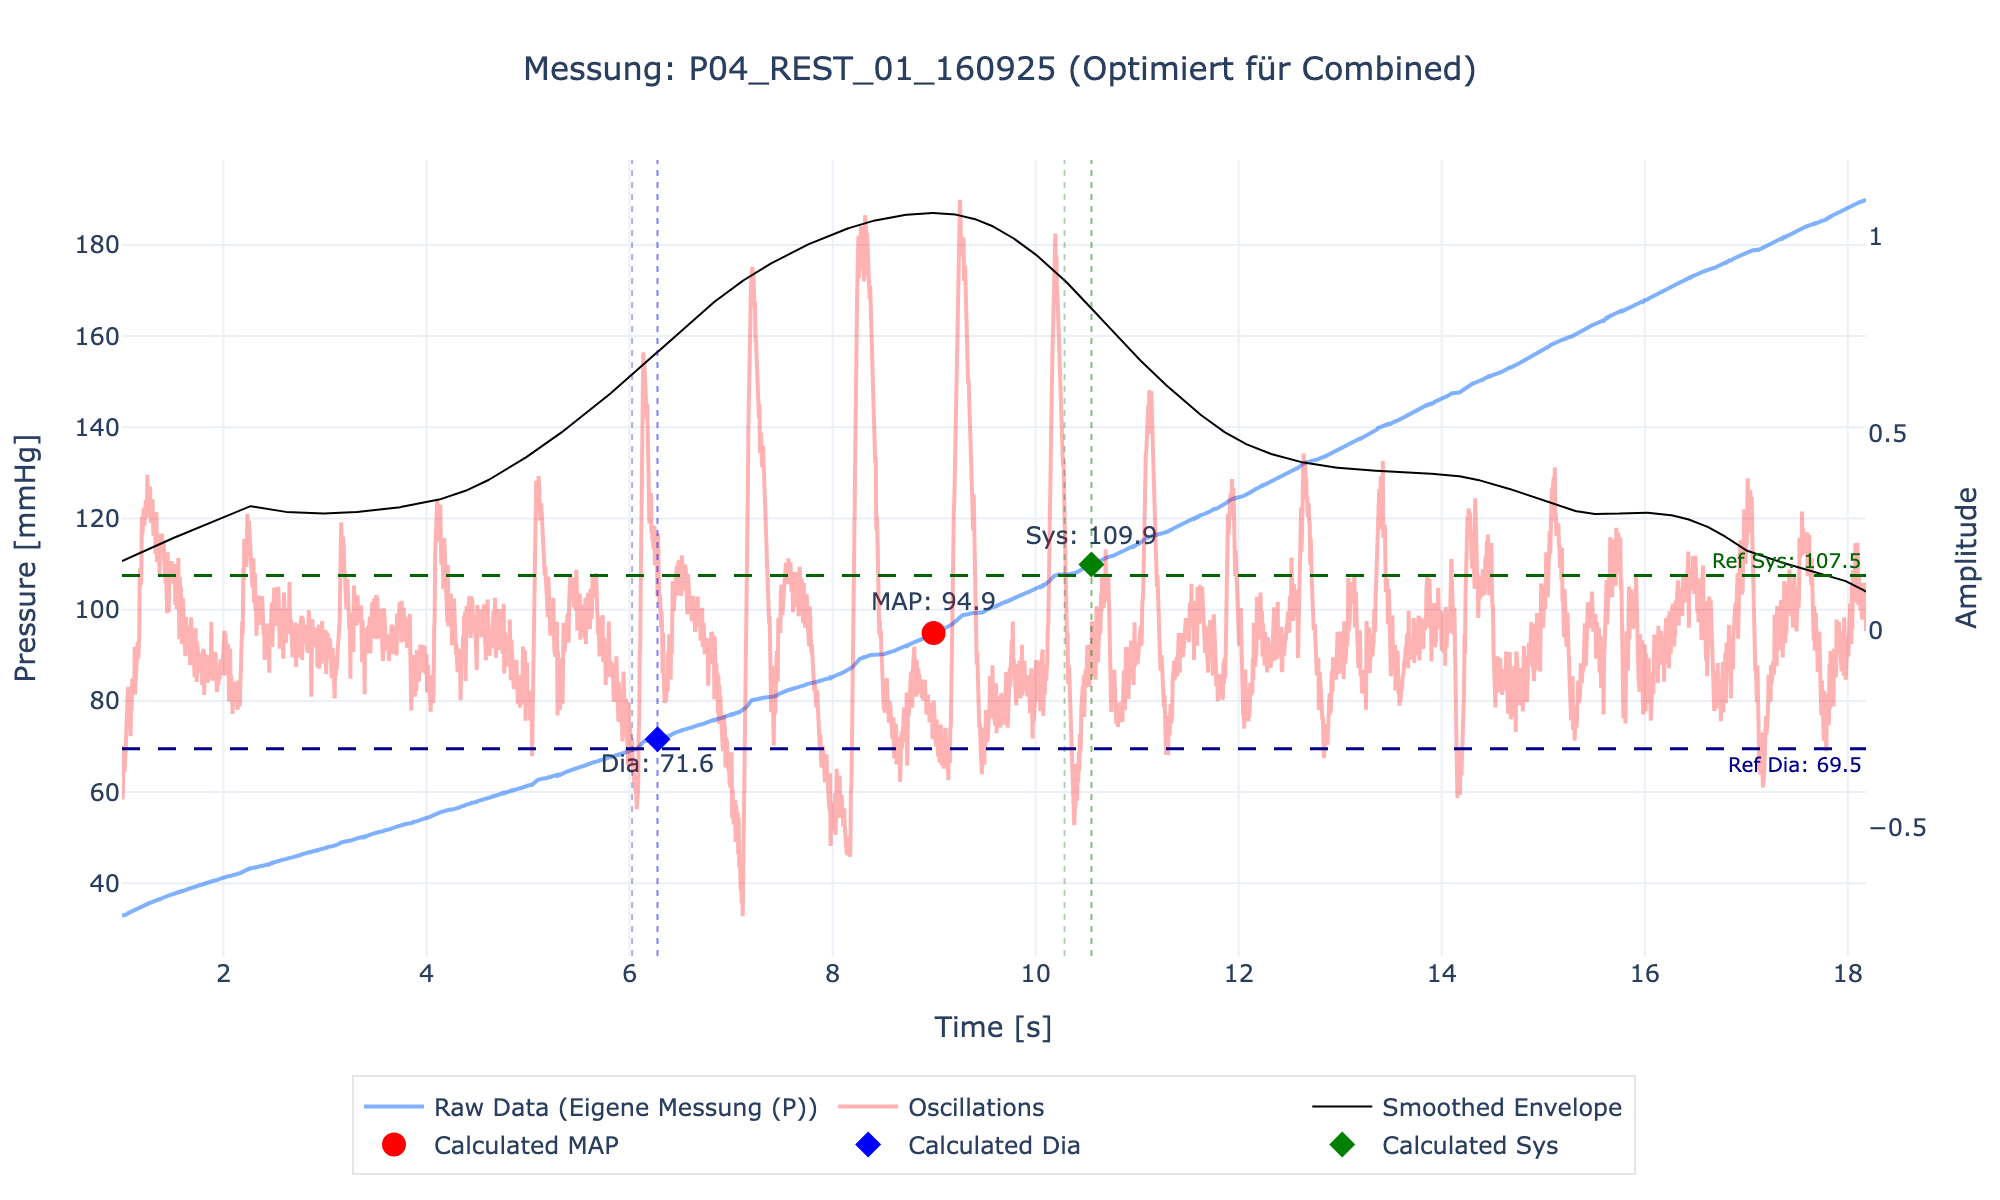
\includegraphics[width=\textwidth]{images/P04_REST_01_160925_combined.png}
        \caption{Optimiert für Beurer und NAIS (Kombiniert)}
    \end{subfigure} \\
    \begin{subfigure}[b]{0.48\textwidth}
        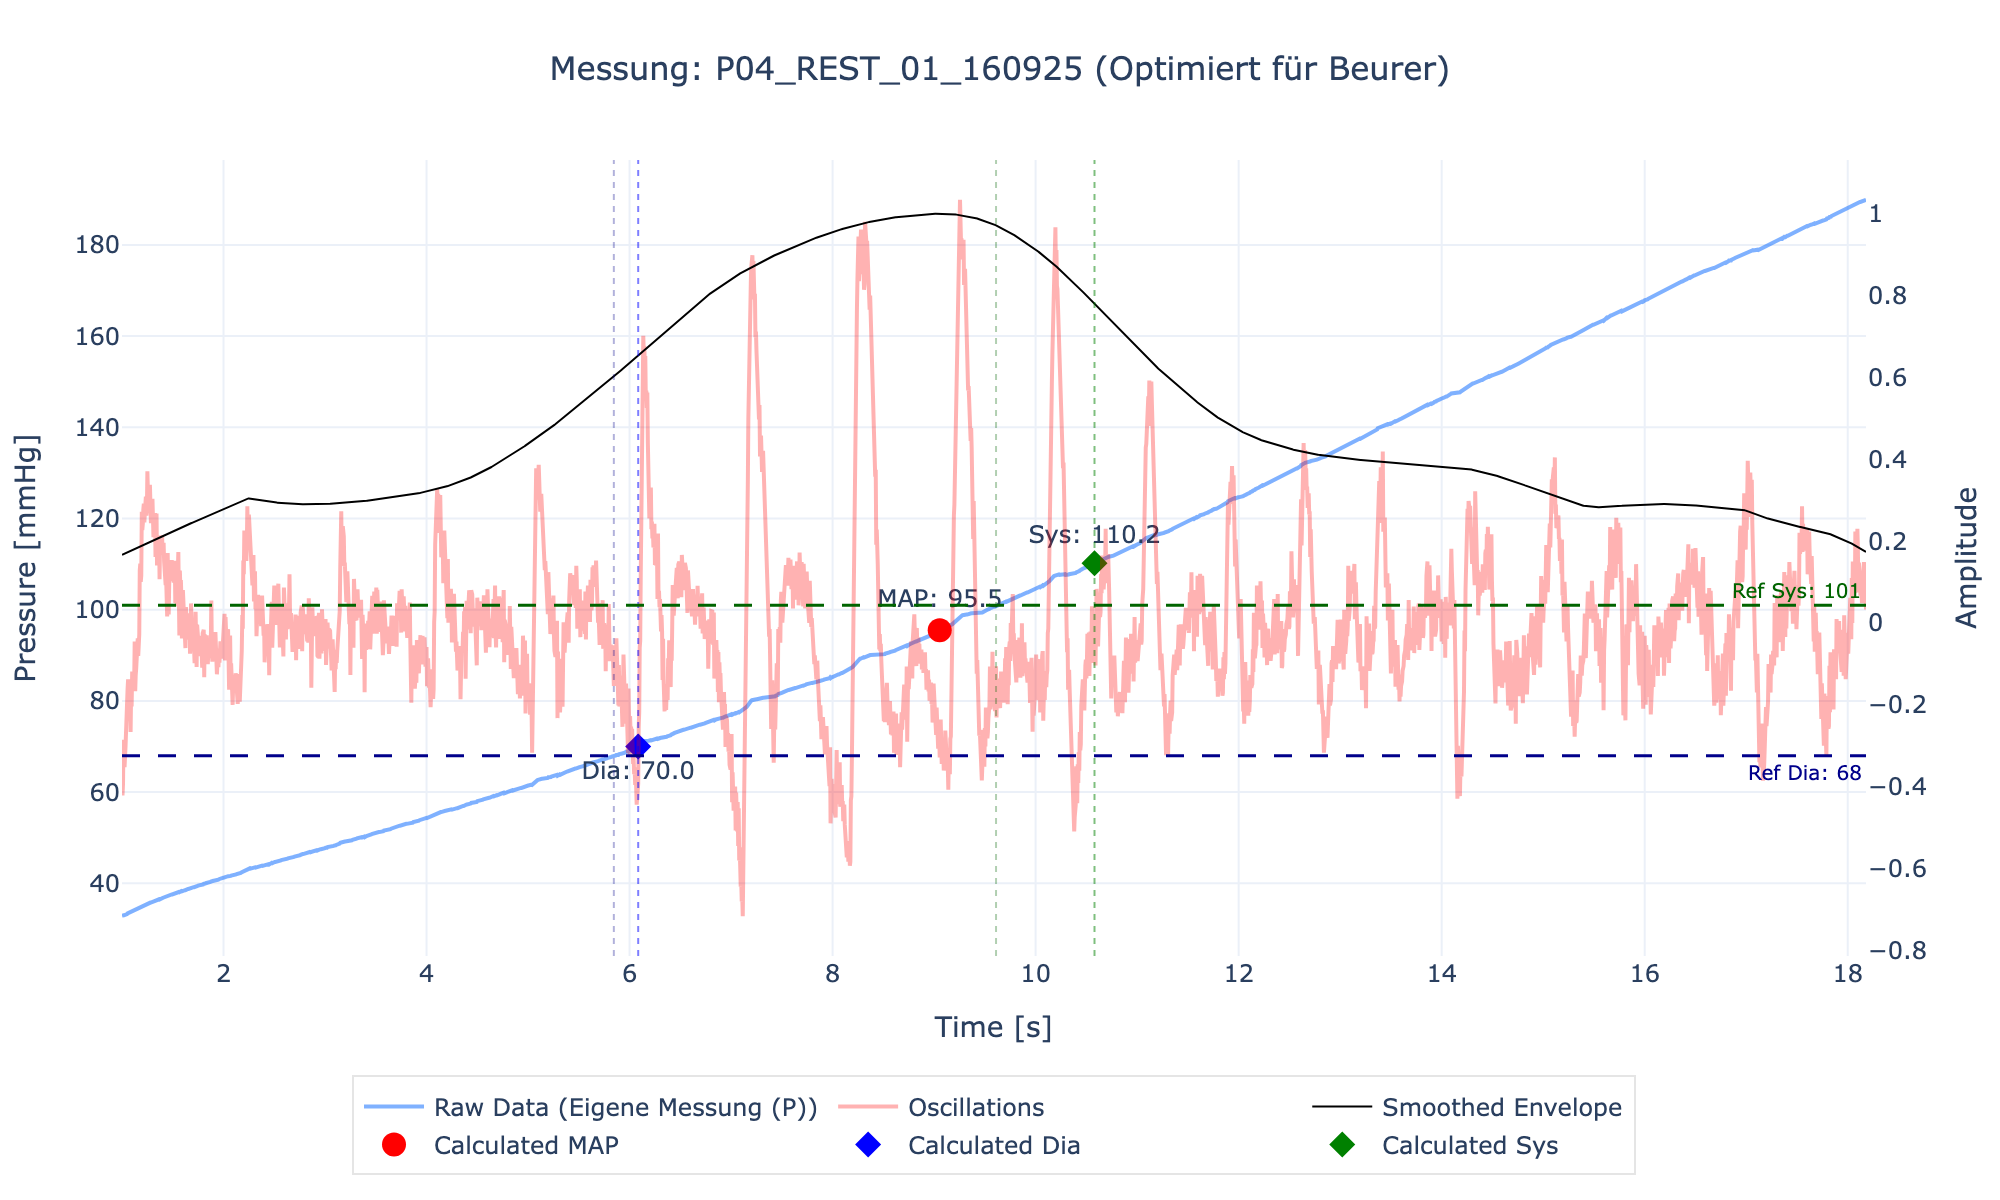
\includegraphics[width=\textwidth]{images/P04_REST_01_160925_beurer.png}
        \caption{Optimiert für Beurer}
    \end{subfigure}
    \hfill
    \begin{subfigure}[b]{0.48\textwidth}
        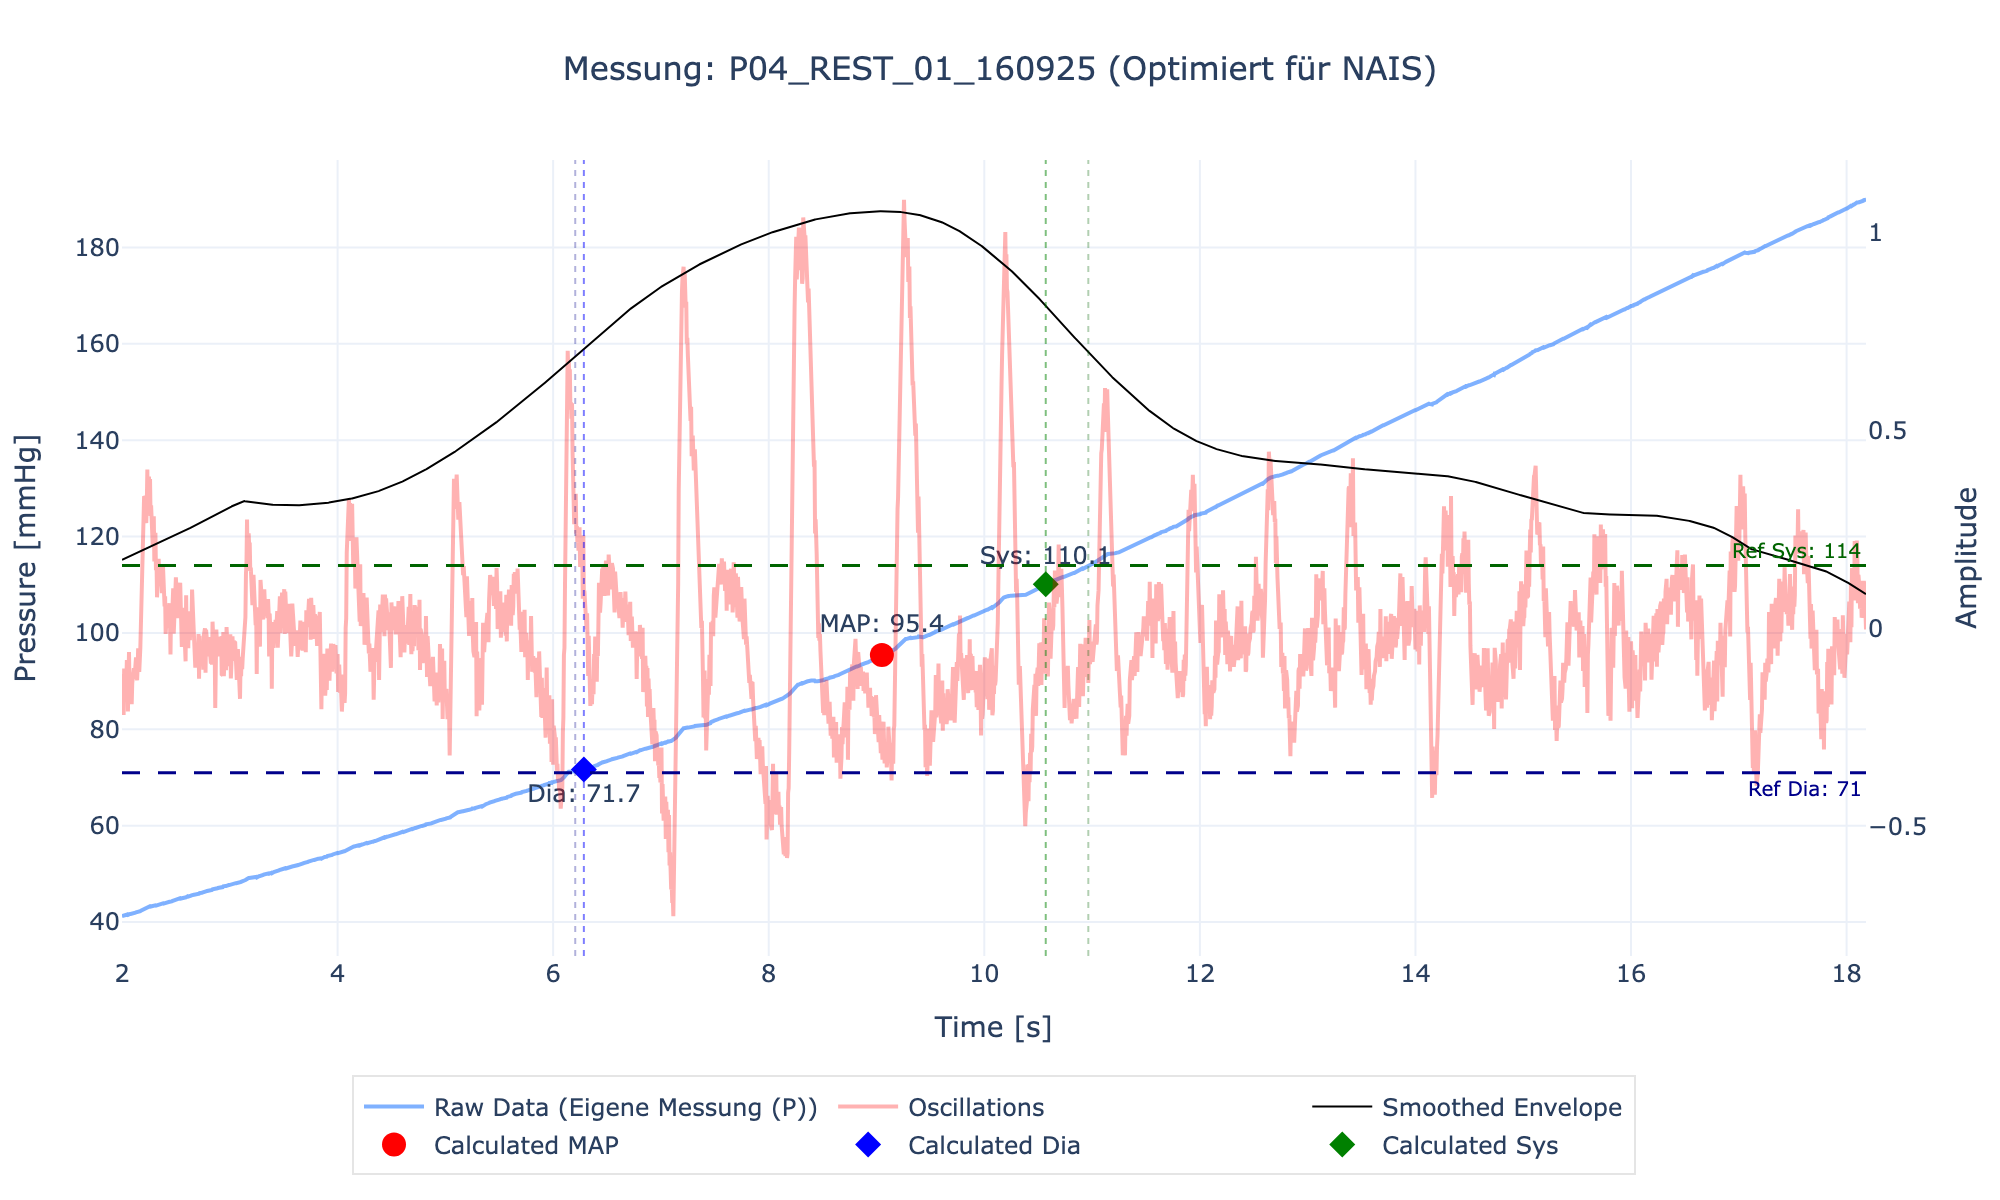
\includegraphics[width=\textwidth]{images/P04_REST_01_160925_nais.png}
        \caption{Optimiert für NAIS}
    \end{subfigure}
    \caption{Einzelauswertung der Messung P04\_REST\_01\_160925 mit verschiedenen Parametersätzen.}
\end{figure}
\newpage

\subsection*{Messung: P05\_ACTIV\_01\_210925}
\begin{figure}[H]
    \centering
    \begin{subfigure}[b]{0.8\textwidth}
        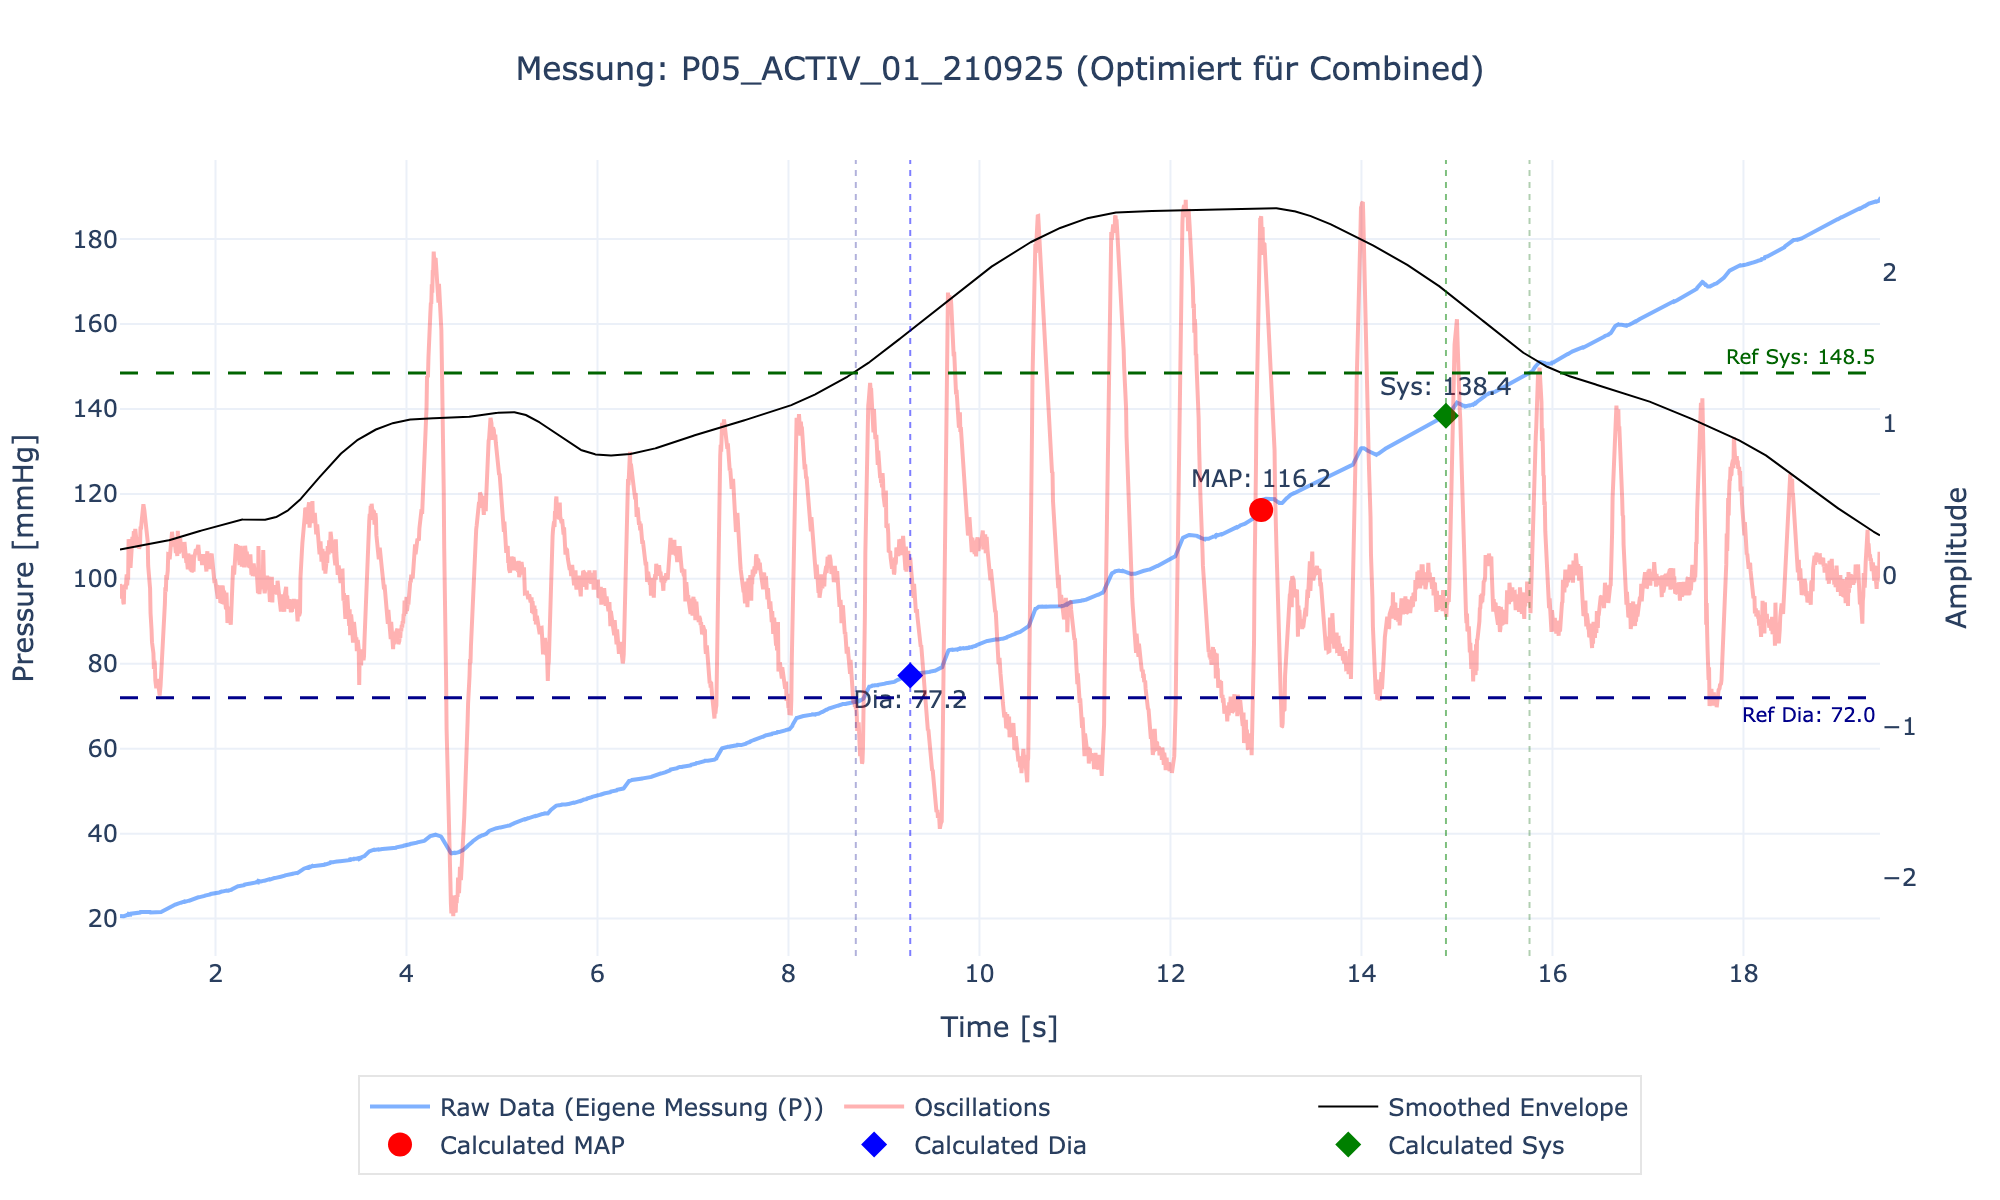
\includegraphics[width=\textwidth]{images/P05_ACTIV_01_210925_combined.png}
        \caption{Optimiert für Beurer und NAIS (Kombiniert)}
    \end{subfigure} \\
    \begin{subfigure}[b]{0.48\textwidth}
        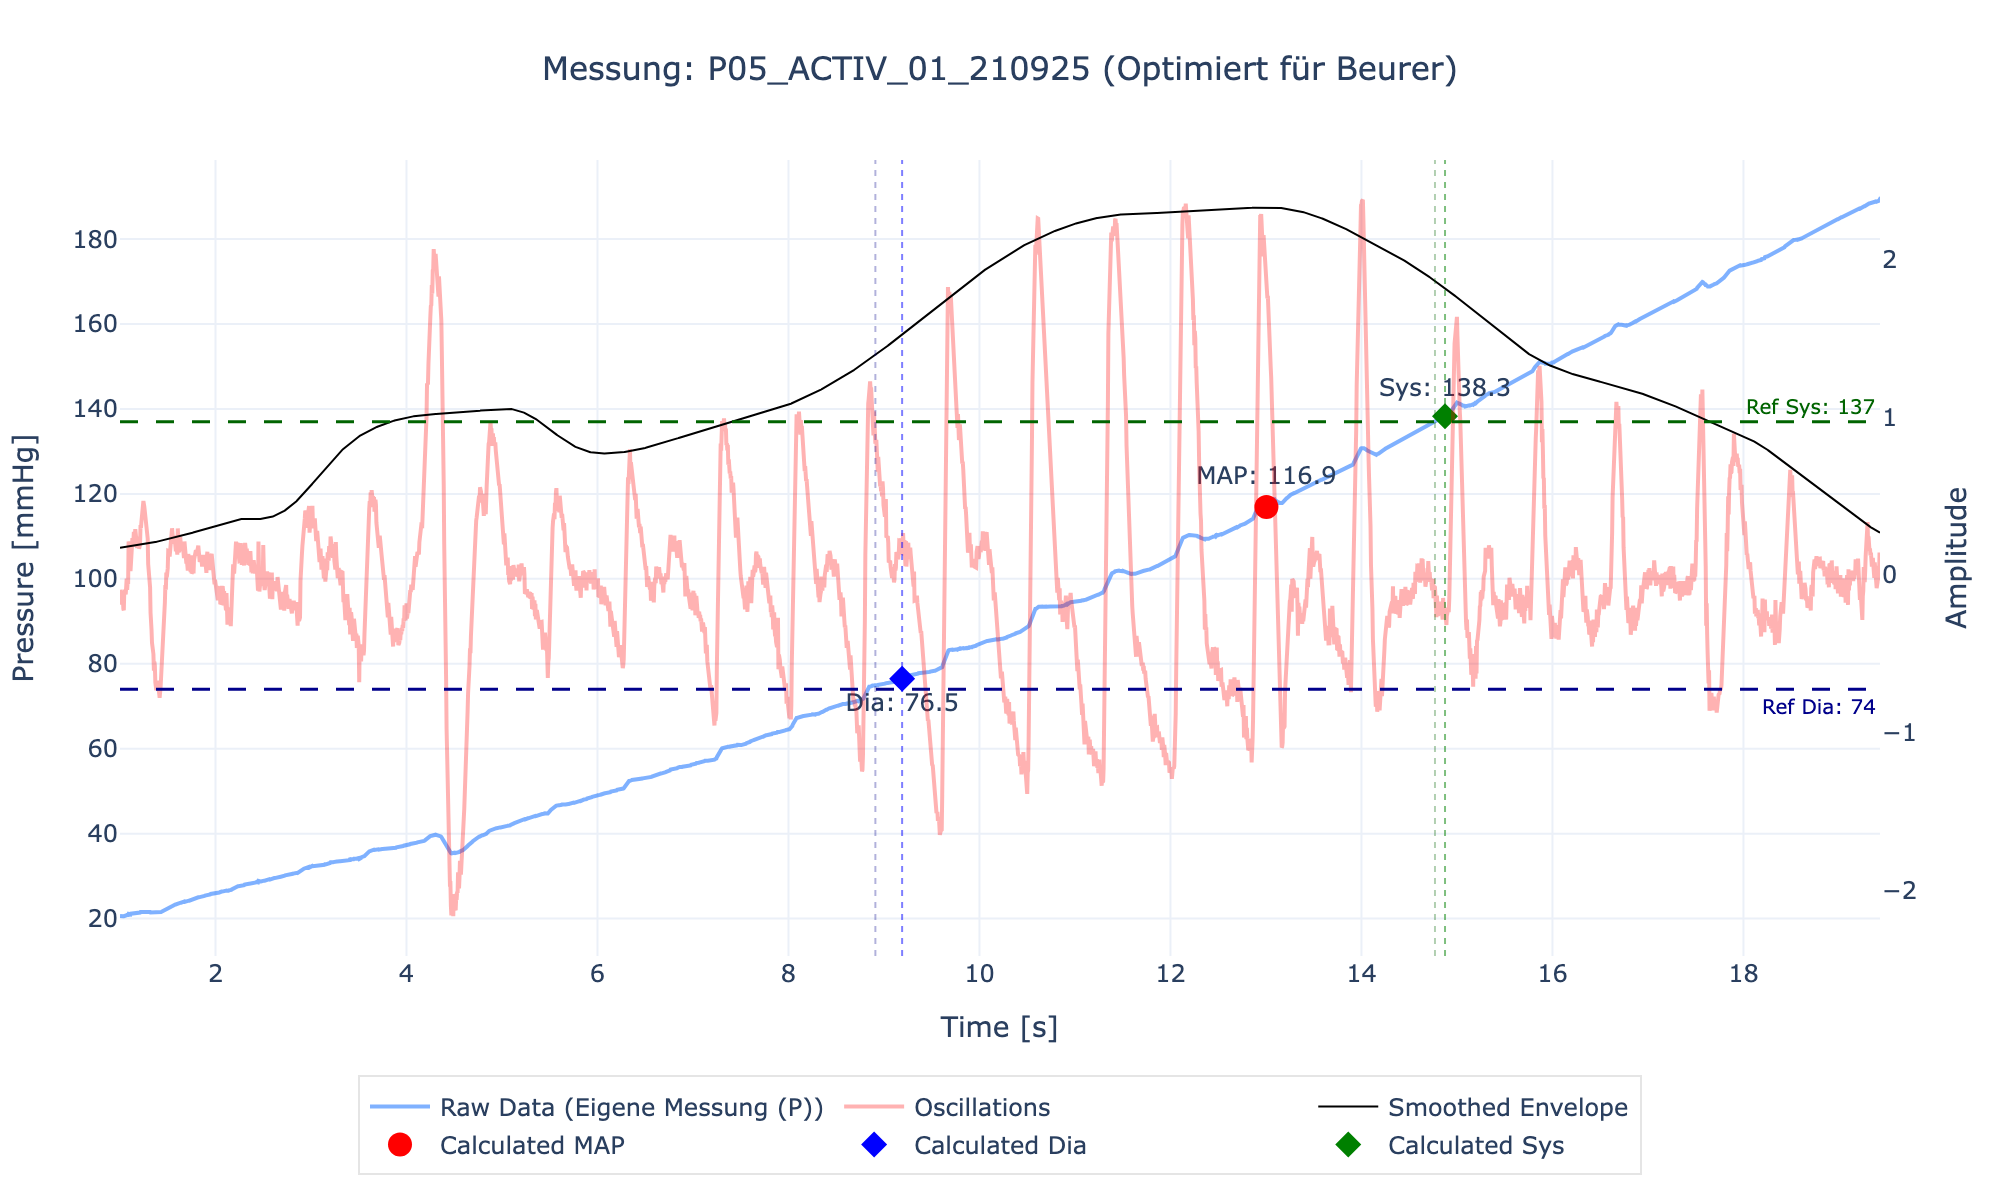
\includegraphics[width=\textwidth]{images/P05_ACTIV_01_210925_beurer.png}
        \caption{Optimiert für Beurer}
    \end{subfigure}
    \hfill
    \begin{subfigure}[b]{0.48\textwidth}
        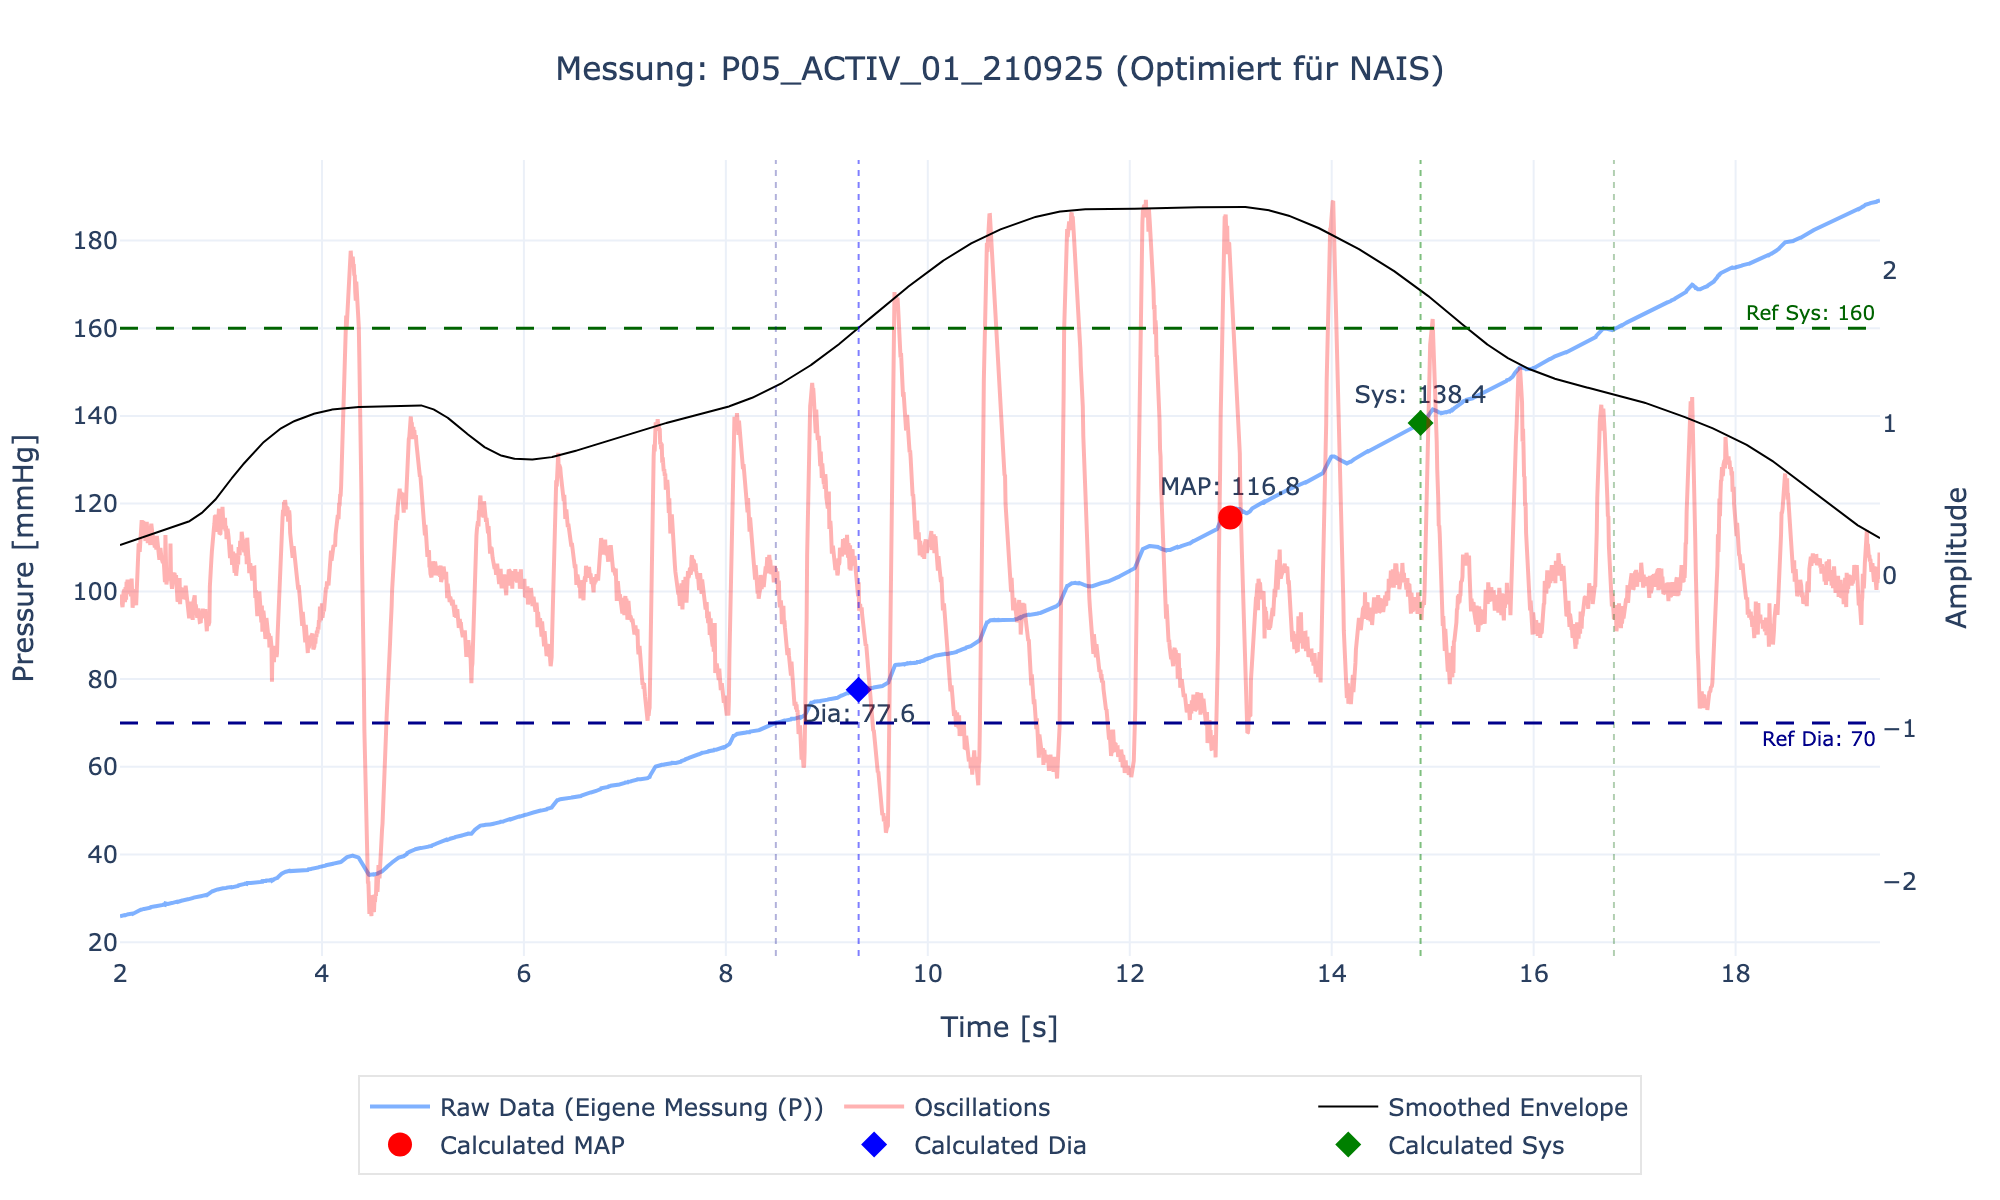
\includegraphics[width=\textwidth]{images/P05_ACTIV_01_210925_nais.png}
        \caption{Optimiert für NAIS}
    \end{subfigure}
    \caption{Einzelauswertung der Messung P05\_ACTIV\_01\_210925 mit verschiedenen Parametersätzen.}
\end{figure}
\newpage

\subsection*{Messung: P05\_REST\_01\_210925}
\begin{figure}[H]
    \centering
    \begin{subfigure}[b]{0.8\textwidth}
        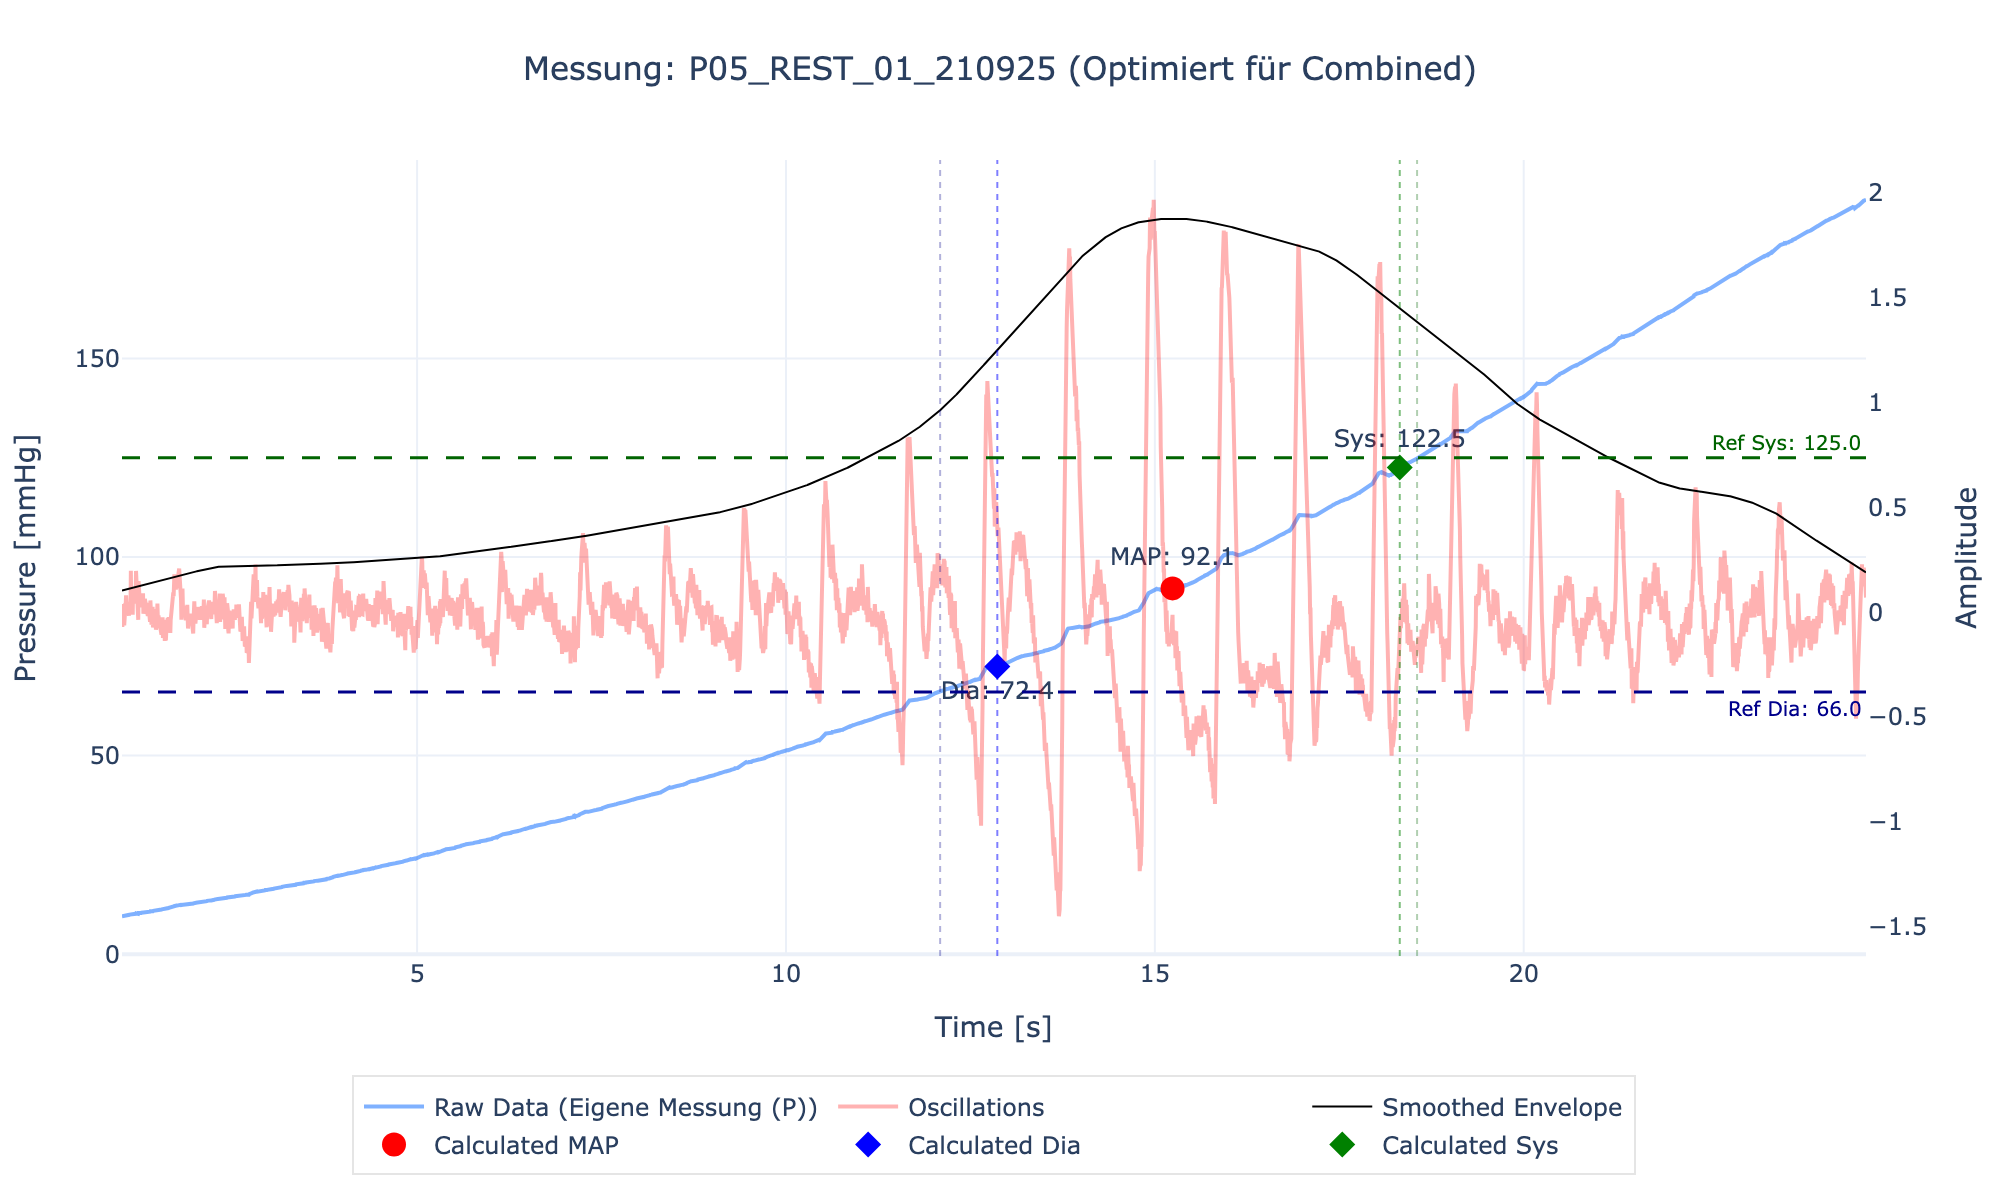
\includegraphics[width=\textwidth]{images/P05_REST_01_210925_combined.png}
        \caption{Optimiert für Beurer und NAIS (Kombiniert)}
    \end{subfigure} \\
    \begin{subfigure}[b]{0.48\textwidth}
        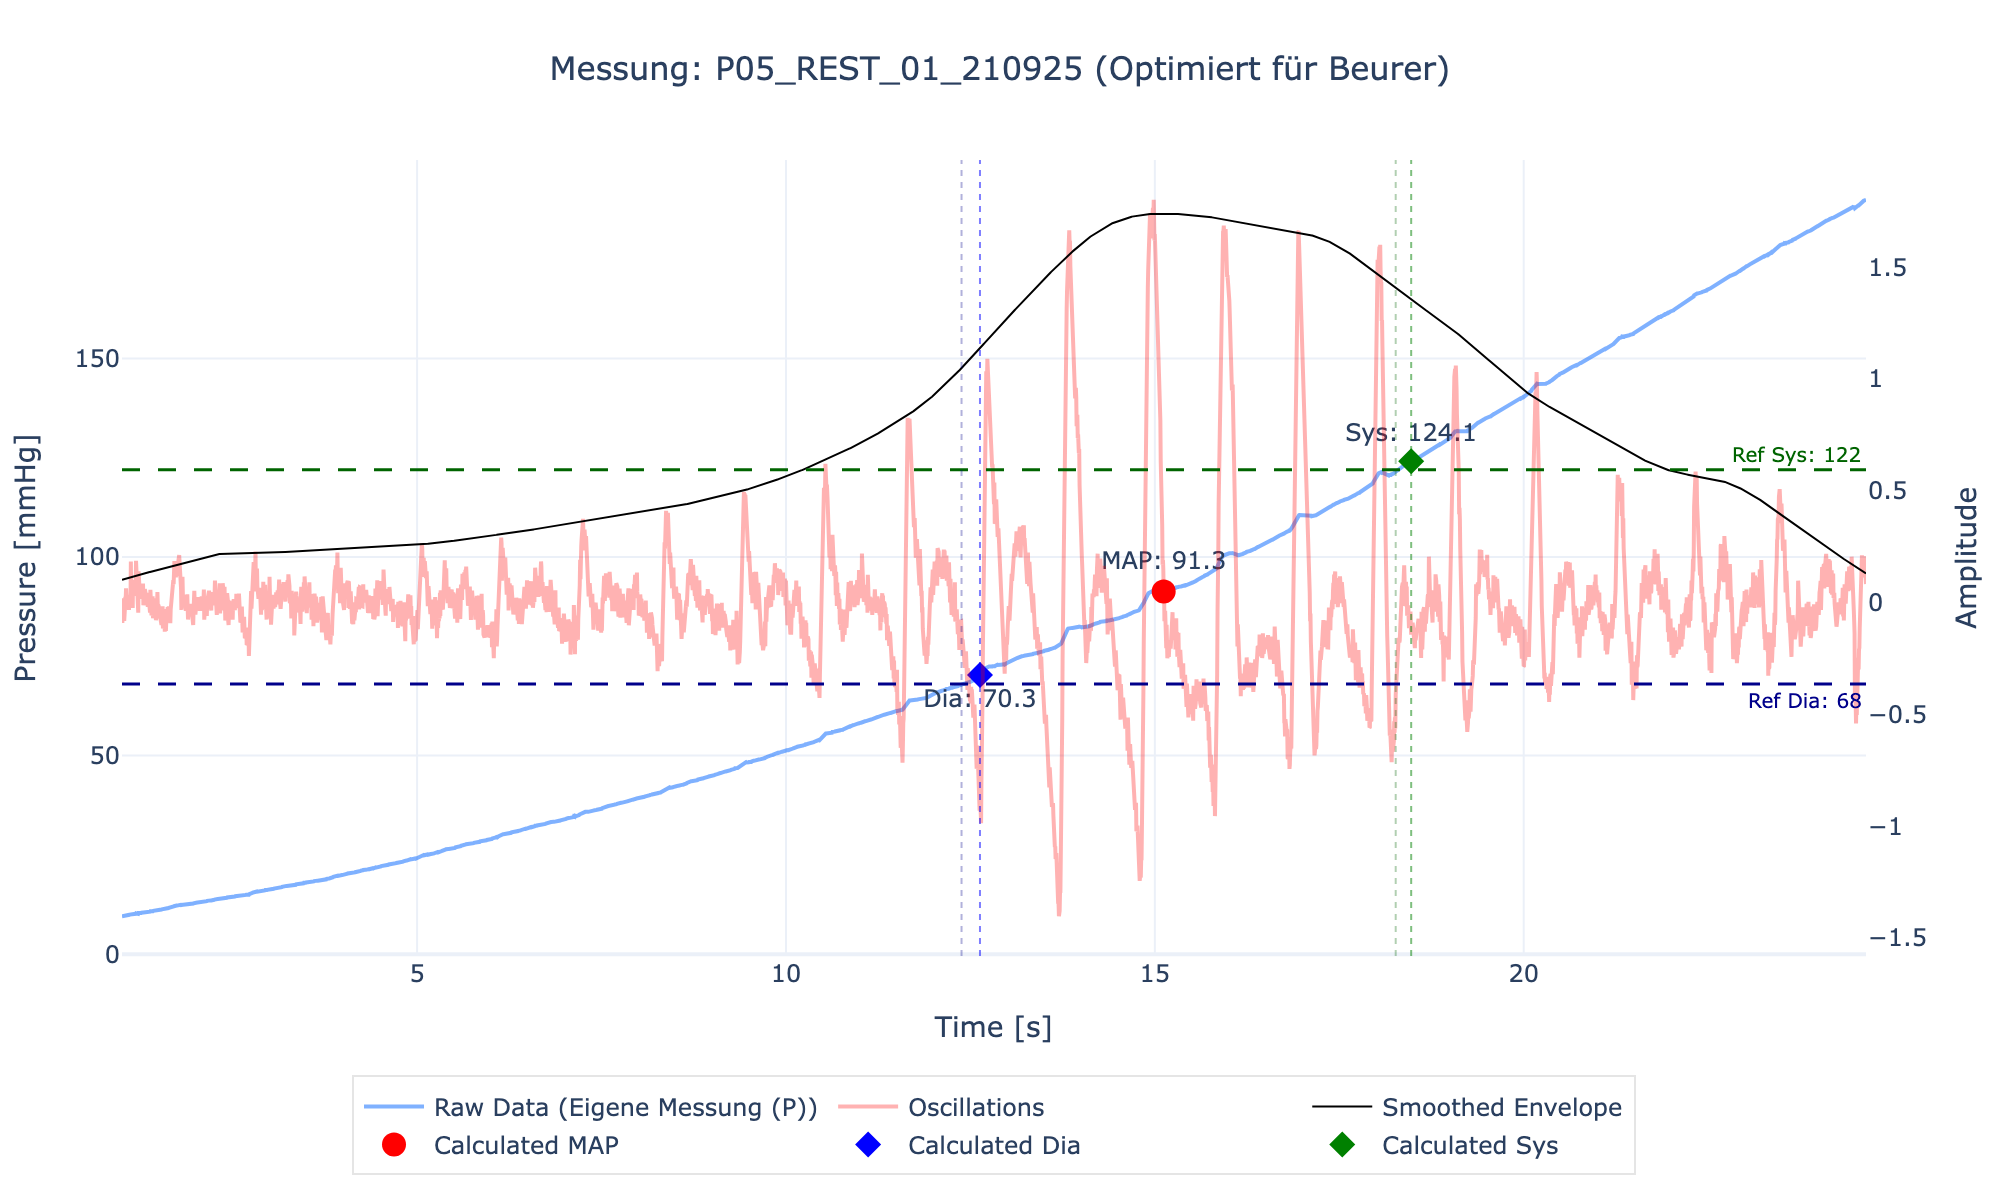
\includegraphics[width=\textwidth]{images/P05_REST_01_210925_beurer.png}
        \caption{Optimiert für Beurer}
    \end{subfigure}
    \hfill
    \begin{subfigure}[b]{0.48\textwidth}
        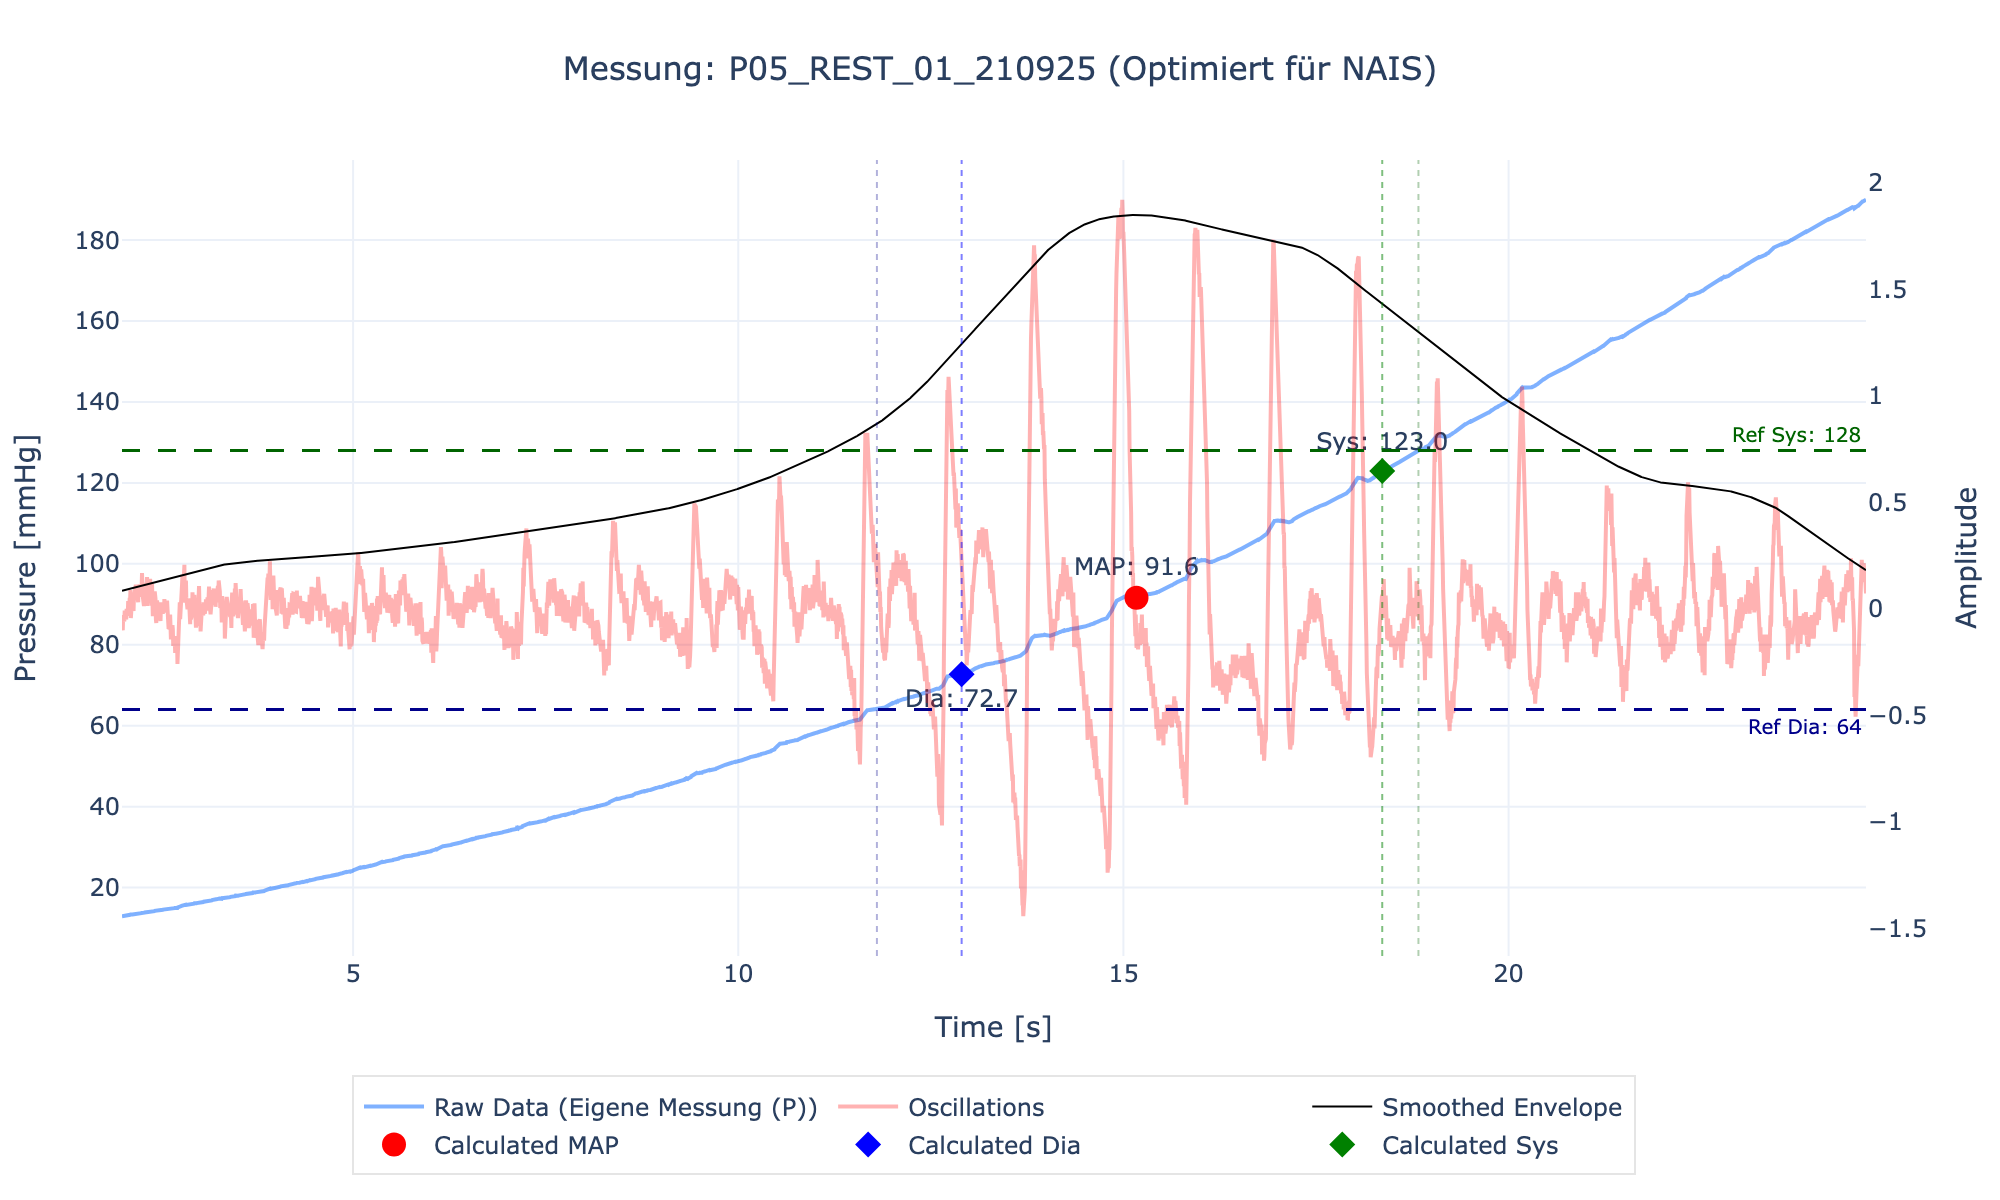
\includegraphics[width=\textwidth]{images/P05_REST_01_210925_nais.png}
        \caption{Optimiert für NAIS}
    \end{subfigure}
    \caption{Einzelauswertung der Messung P05\_REST\_01\_210925 mit verschiedenen Parametersätzen.}
\end{figure}
\newpage

\subsection*{Messung: P06\_ACTIV\_01\_191025}
\begin{figure}[H]
    \centering
    \begin{subfigure}[b]{0.8\textwidth}
        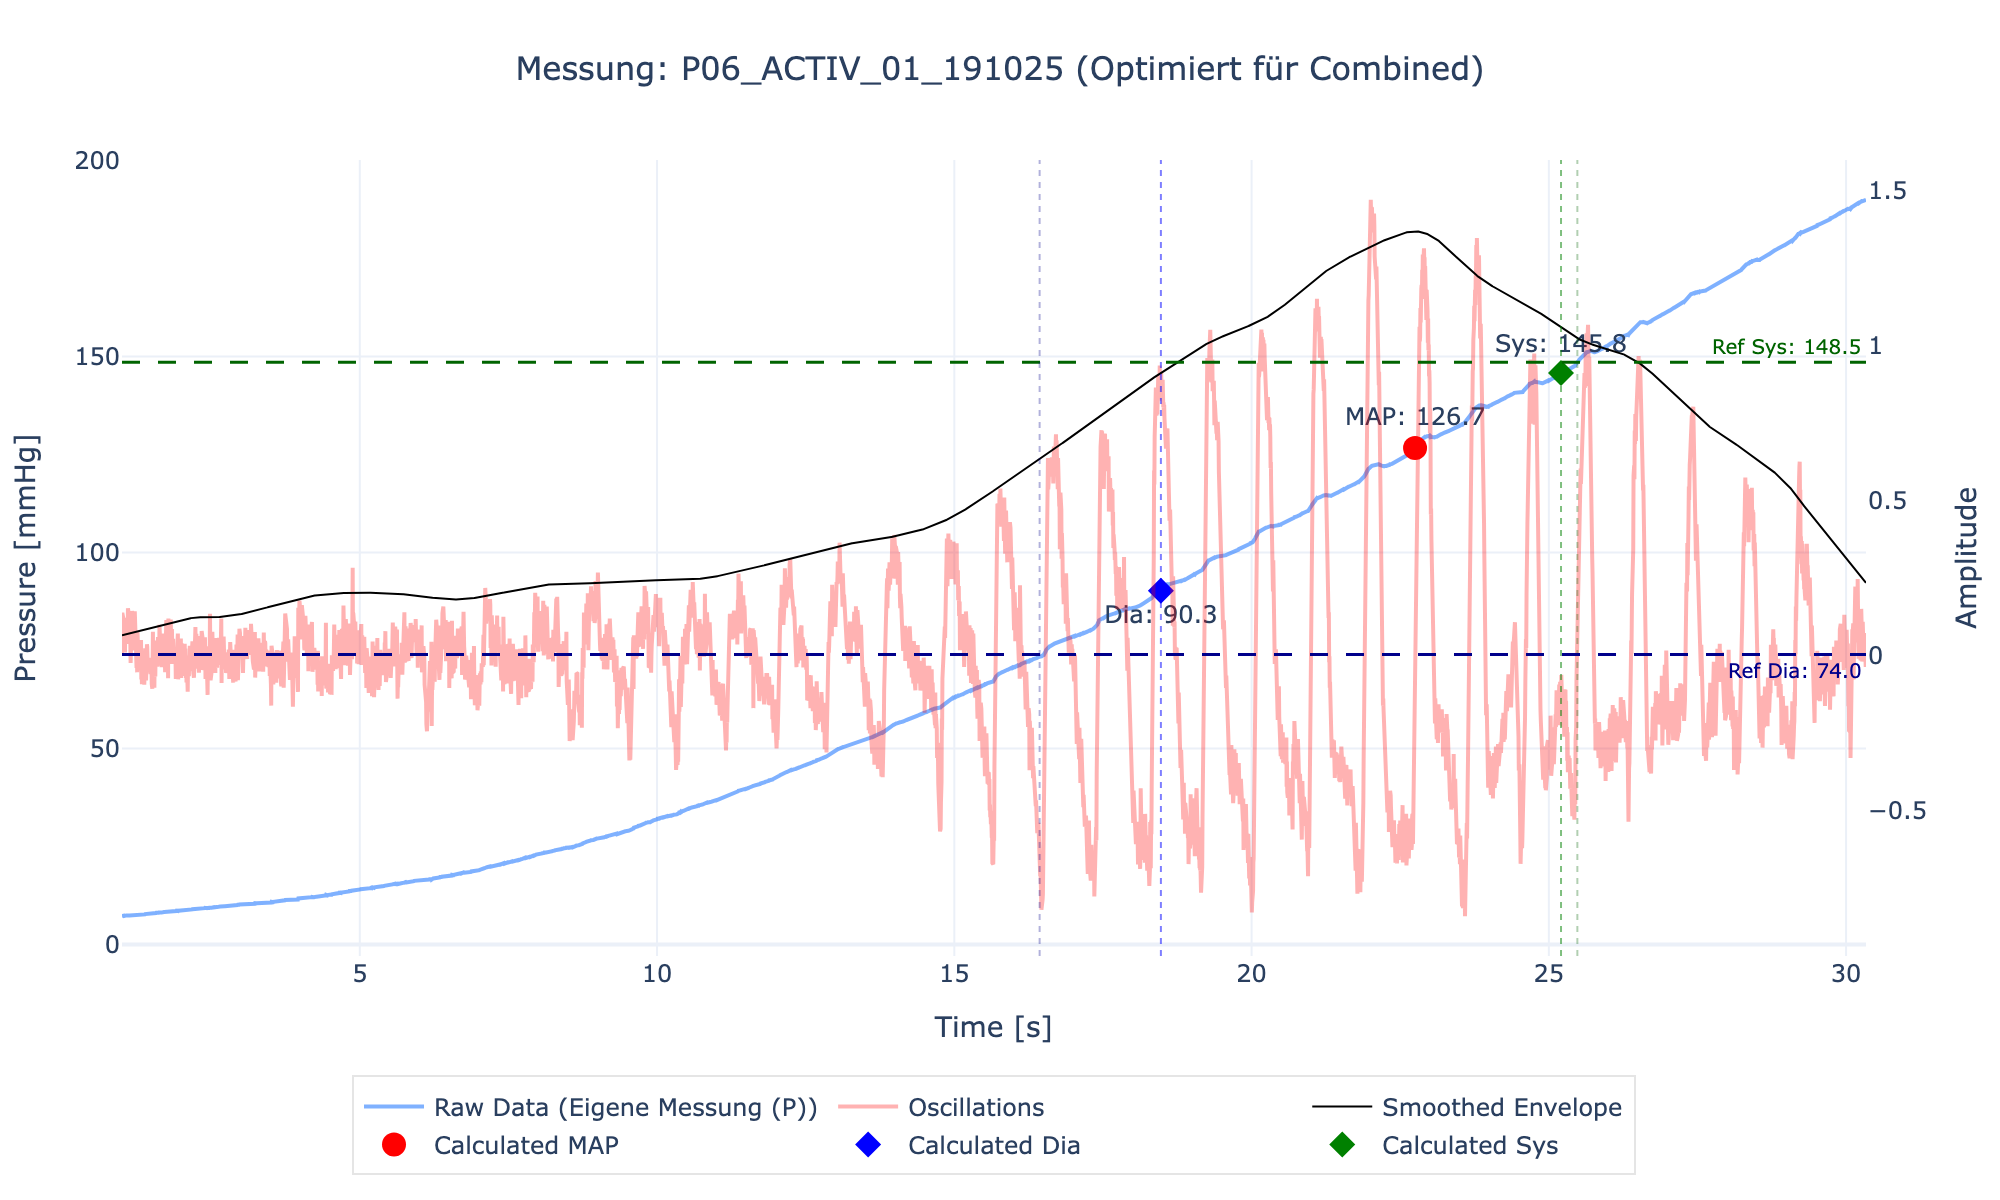
\includegraphics[width=\textwidth]{images/P06_ACTIV_01_191025_combined.png}
        \caption{Optimiert für Beurer und NAIS (Kombiniert)}
    \end{subfigure} \\
    \begin{subfigure}[b]{0.48\textwidth}
        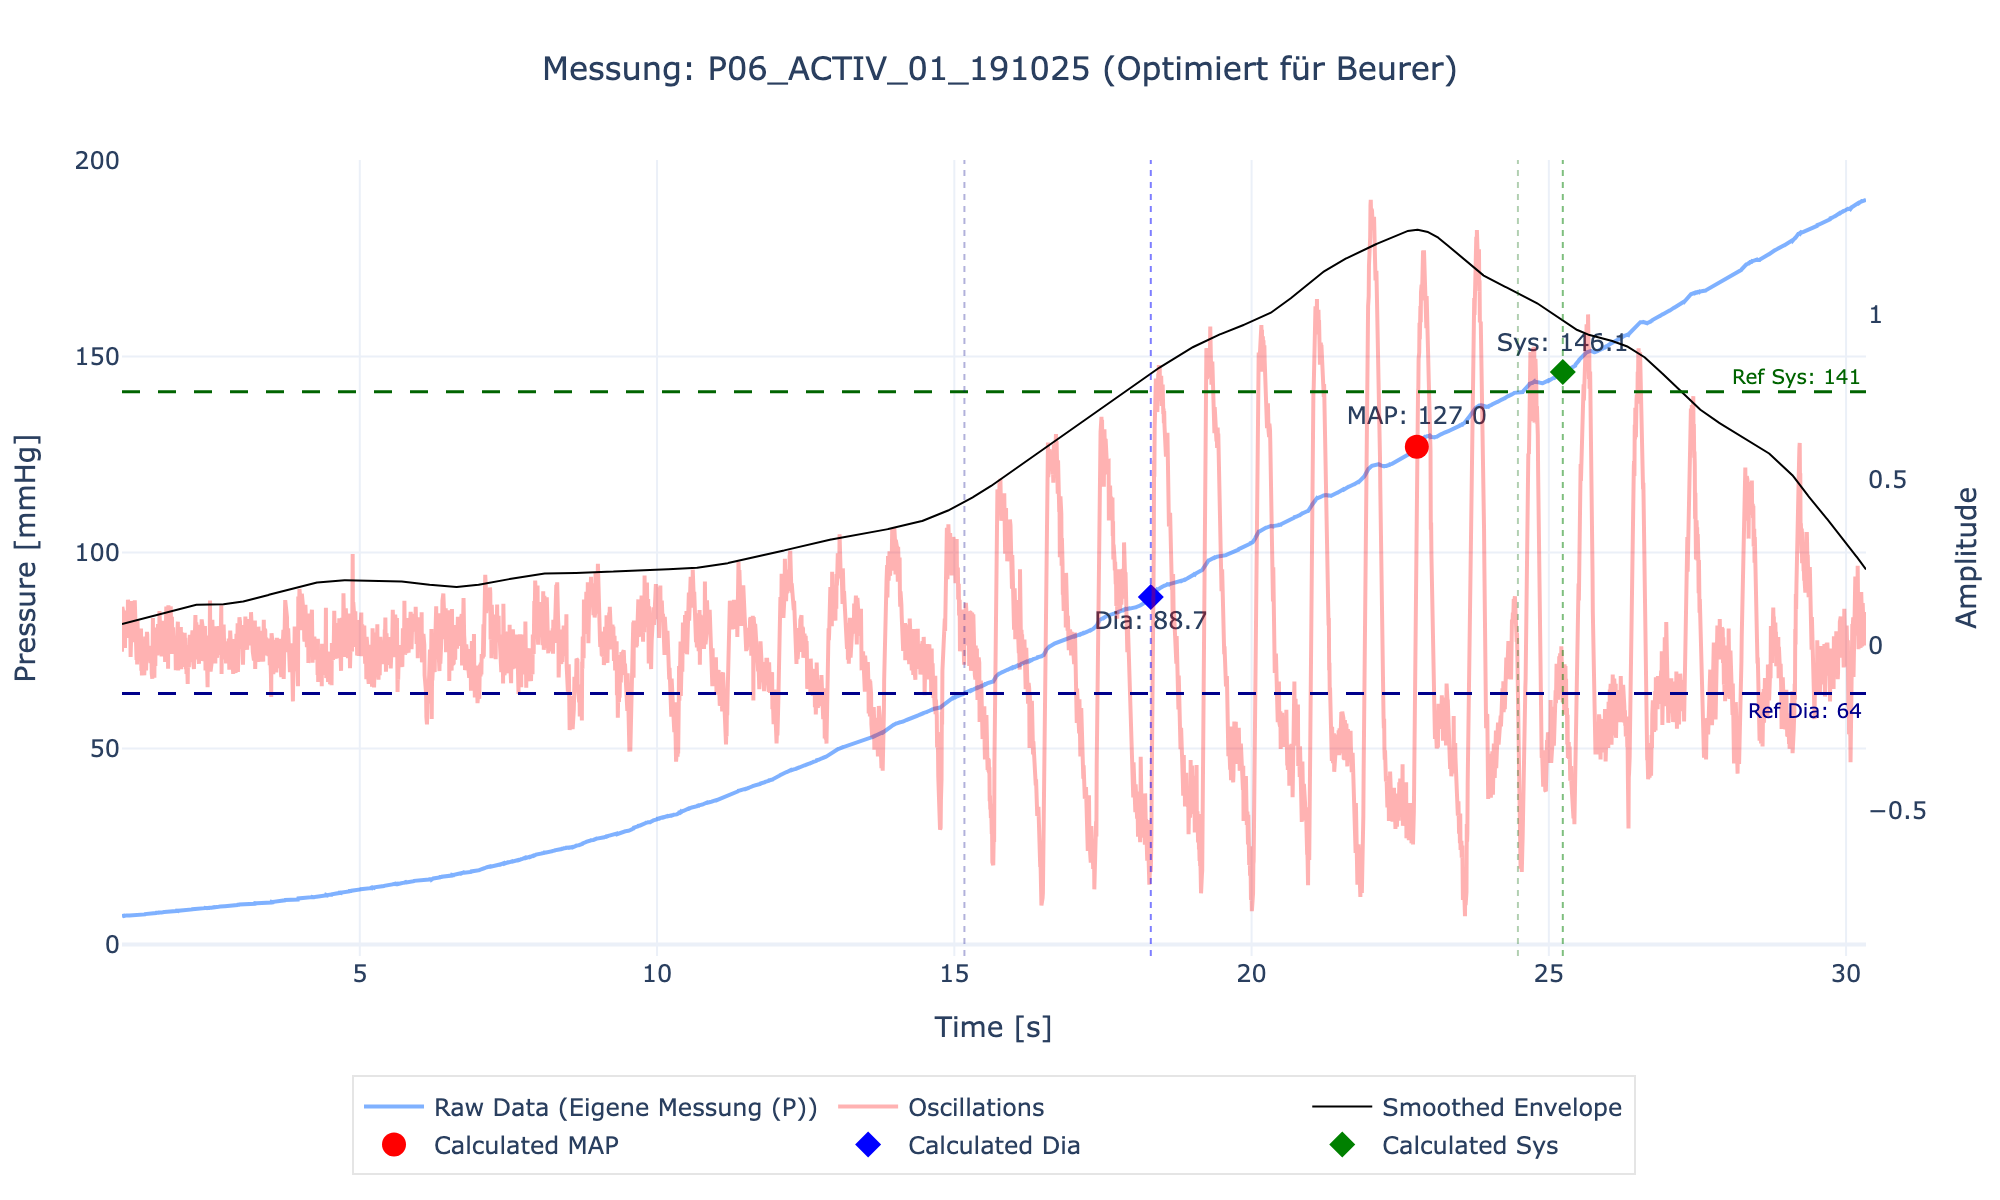
\includegraphics[width=\textwidth]{images/P06_ACTIV_01_191025_beurer.png}
        \caption{Optimiert für Beurer}
    \end{subfigure}
    \hfill
    \begin{subfigure}[b]{0.48\textwidth}
        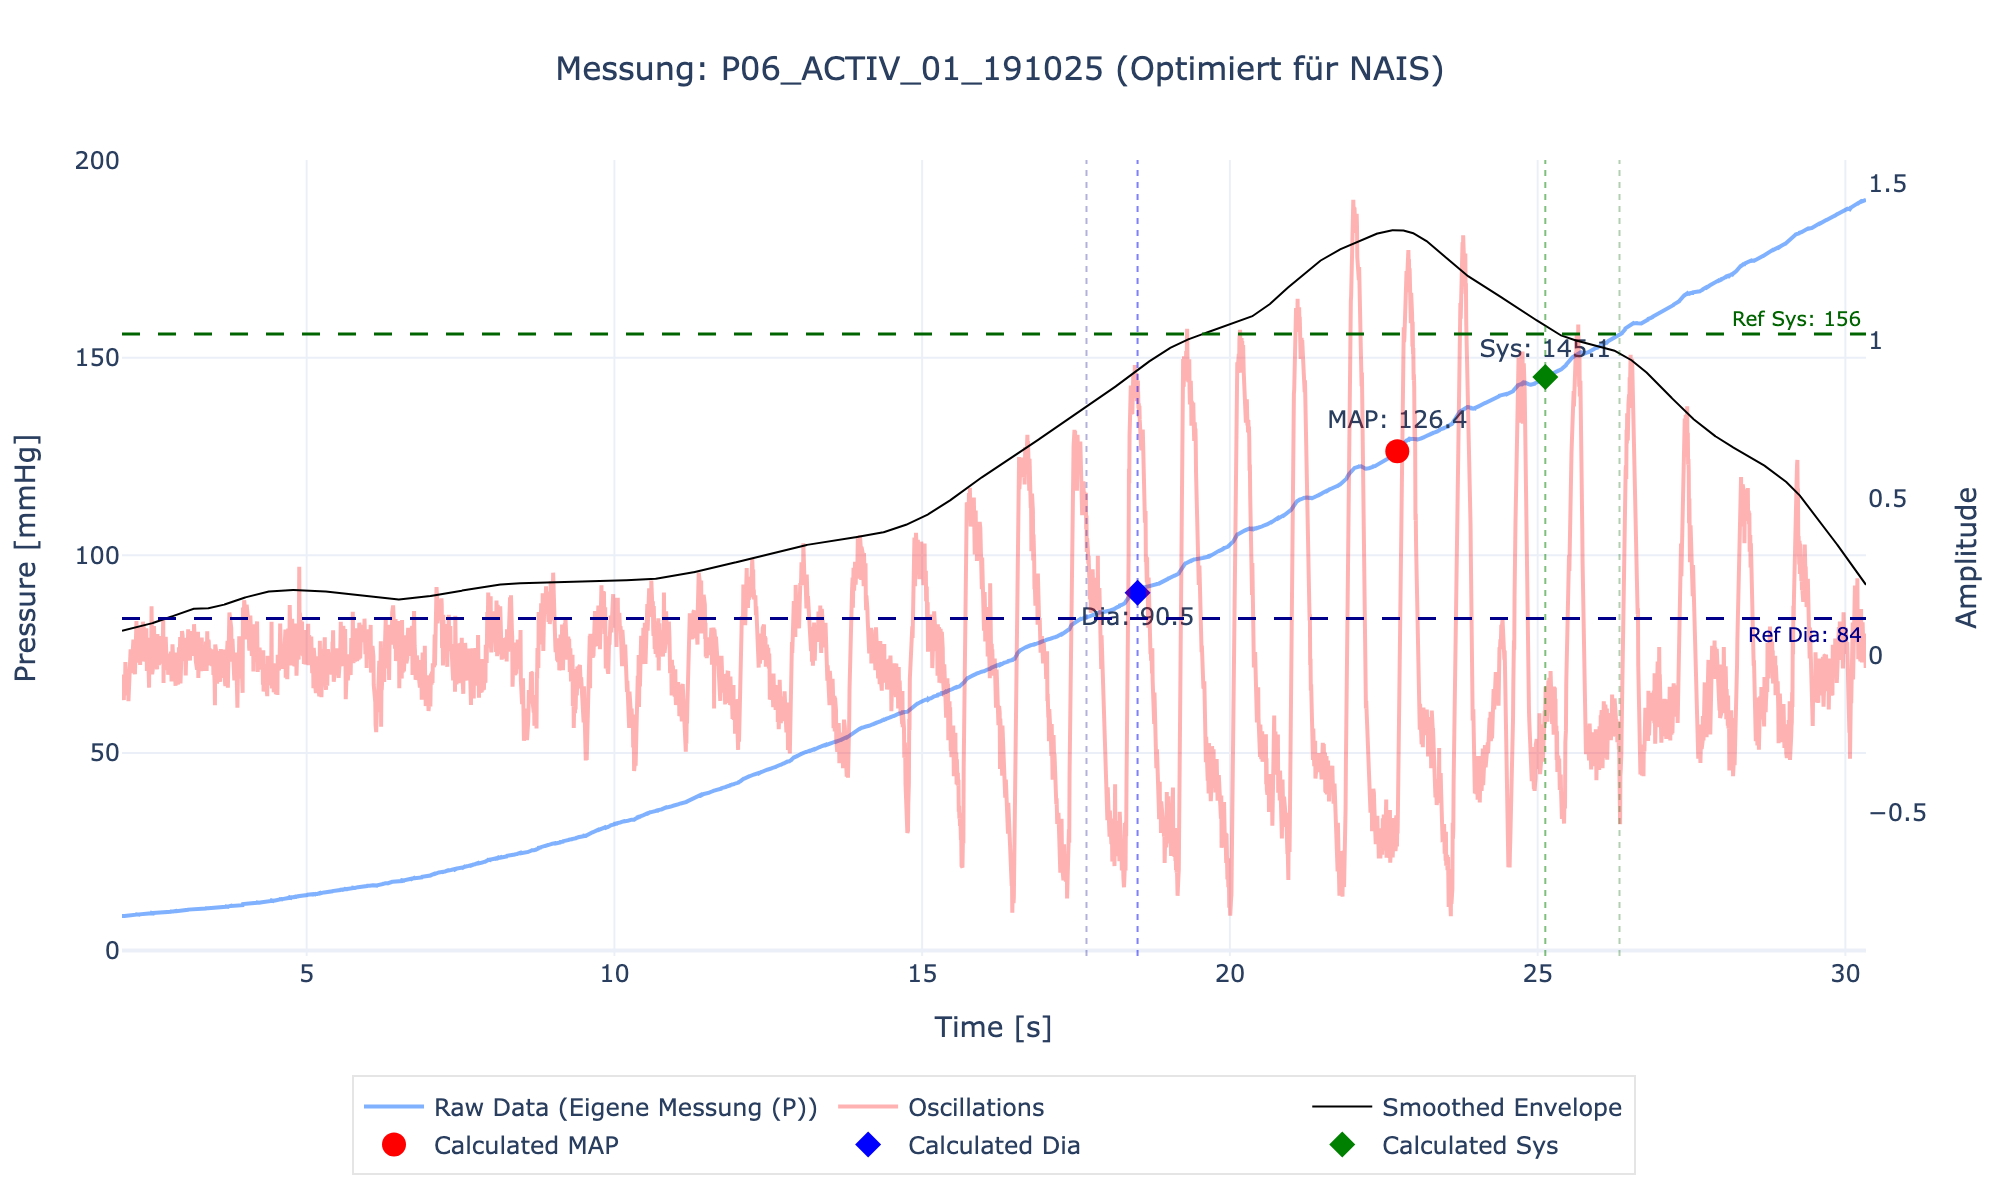
\includegraphics[width=\textwidth]{images/P06_ACTIV_01_191025_nais.png}
        \caption{Optimiert für NAIS}
    \end{subfigure}
    \caption{Einzelauswertung der Messung P06\_ACTIV\_01\_191025 mit verschiedenen Parametersätzen.}
\end{figure}
\newpage

\subsection*{Messung: P06\_REST\_01\_191025}
\begin{figure}[H]
    \centering
    \begin{subfigure}[b]{0.8\textwidth}
        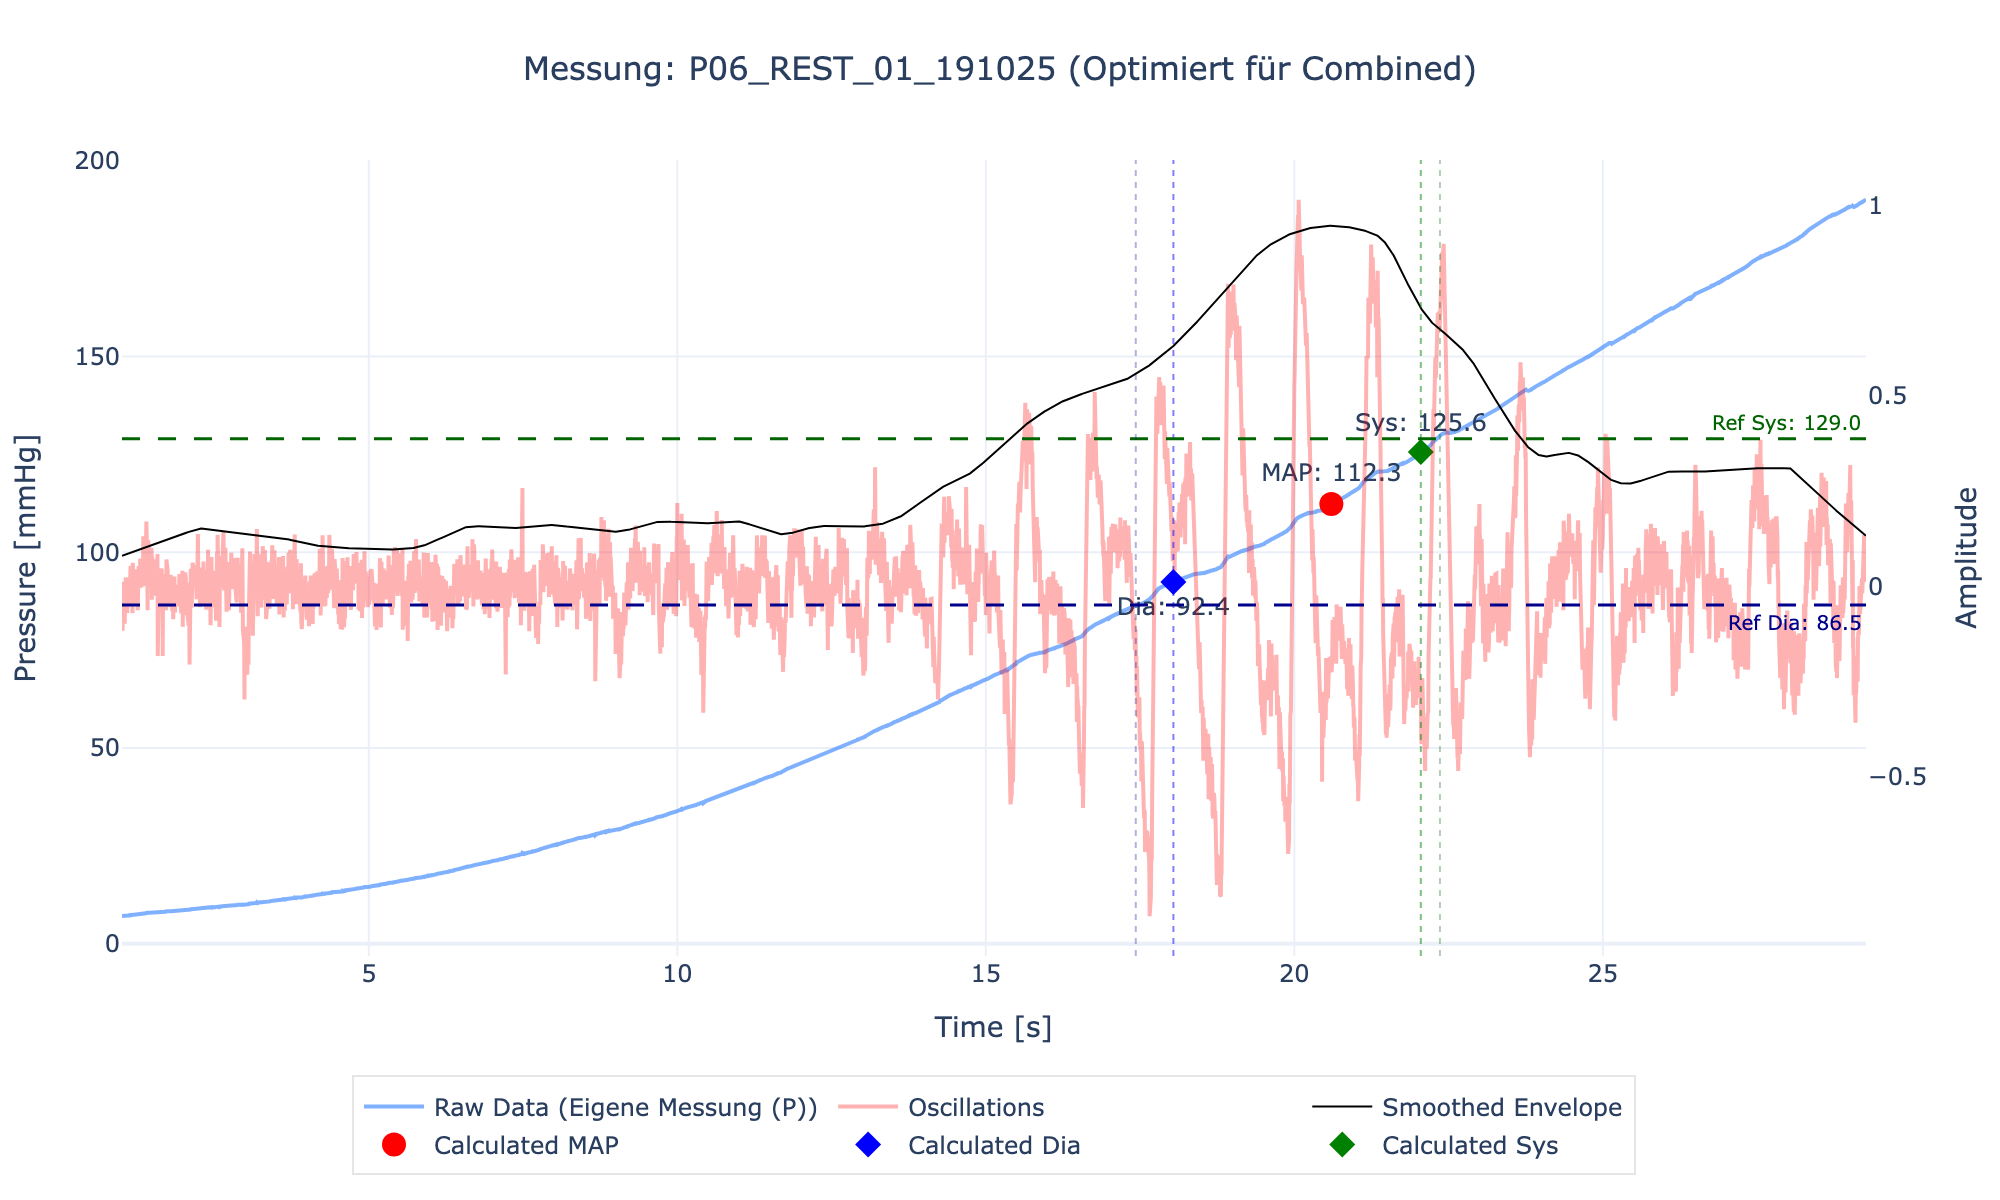
\includegraphics[width=\textwidth]{images/P06_REST_01_191025_combined.png}
        \caption{Optimiert für Beurer und NAIS (Kombiniert)}
    \end{subfigure} \\
    \begin{subfigure}[b]{0.48\textwidth}
        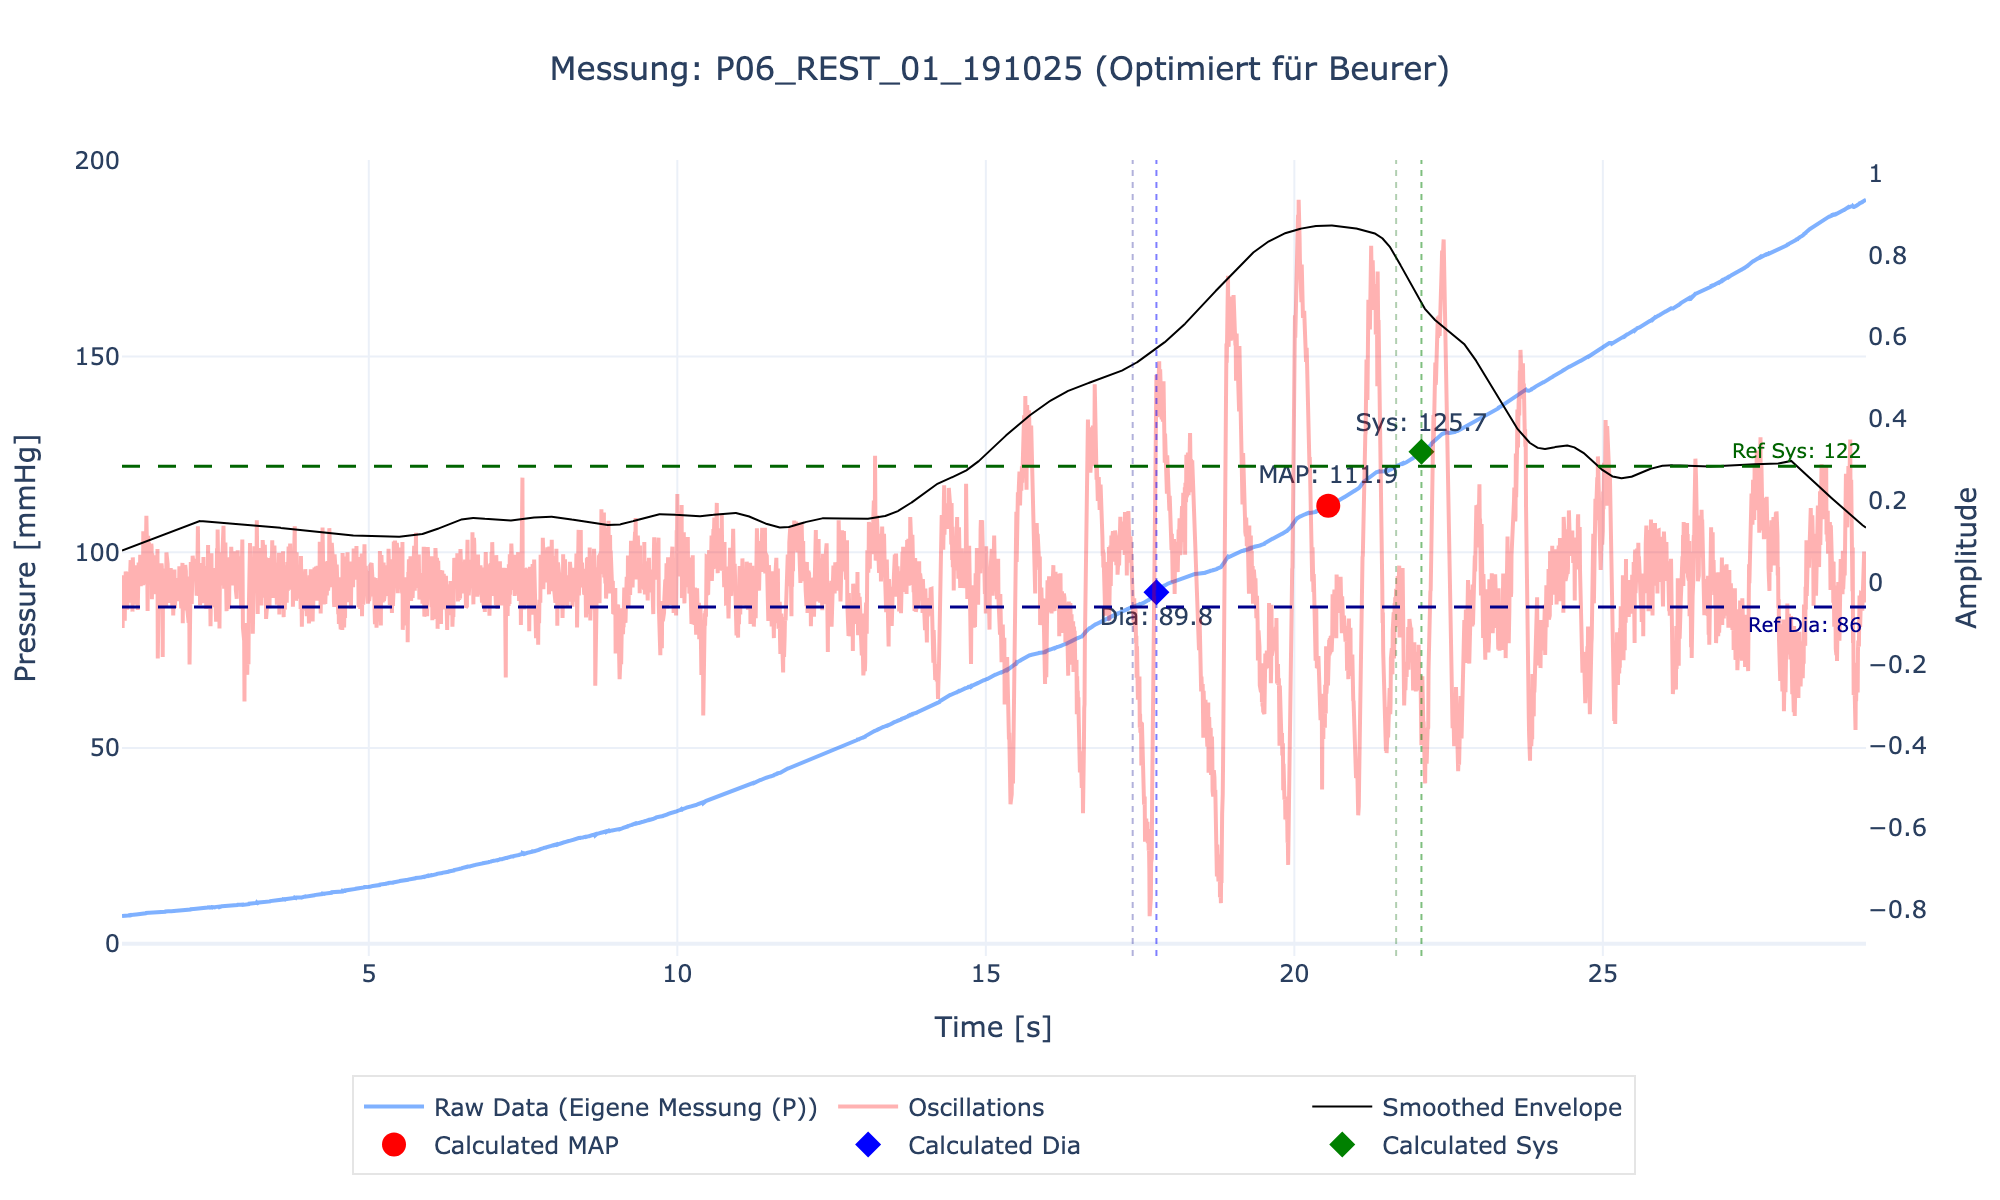
\includegraphics[width=\textwidth]{images/P06_REST_01_191025_beurer.png}
        \caption{Optimiert für Beurer}
    \end{subfigure}
    \hfill
    \begin{subfigure}[b]{0.48\textwidth}
        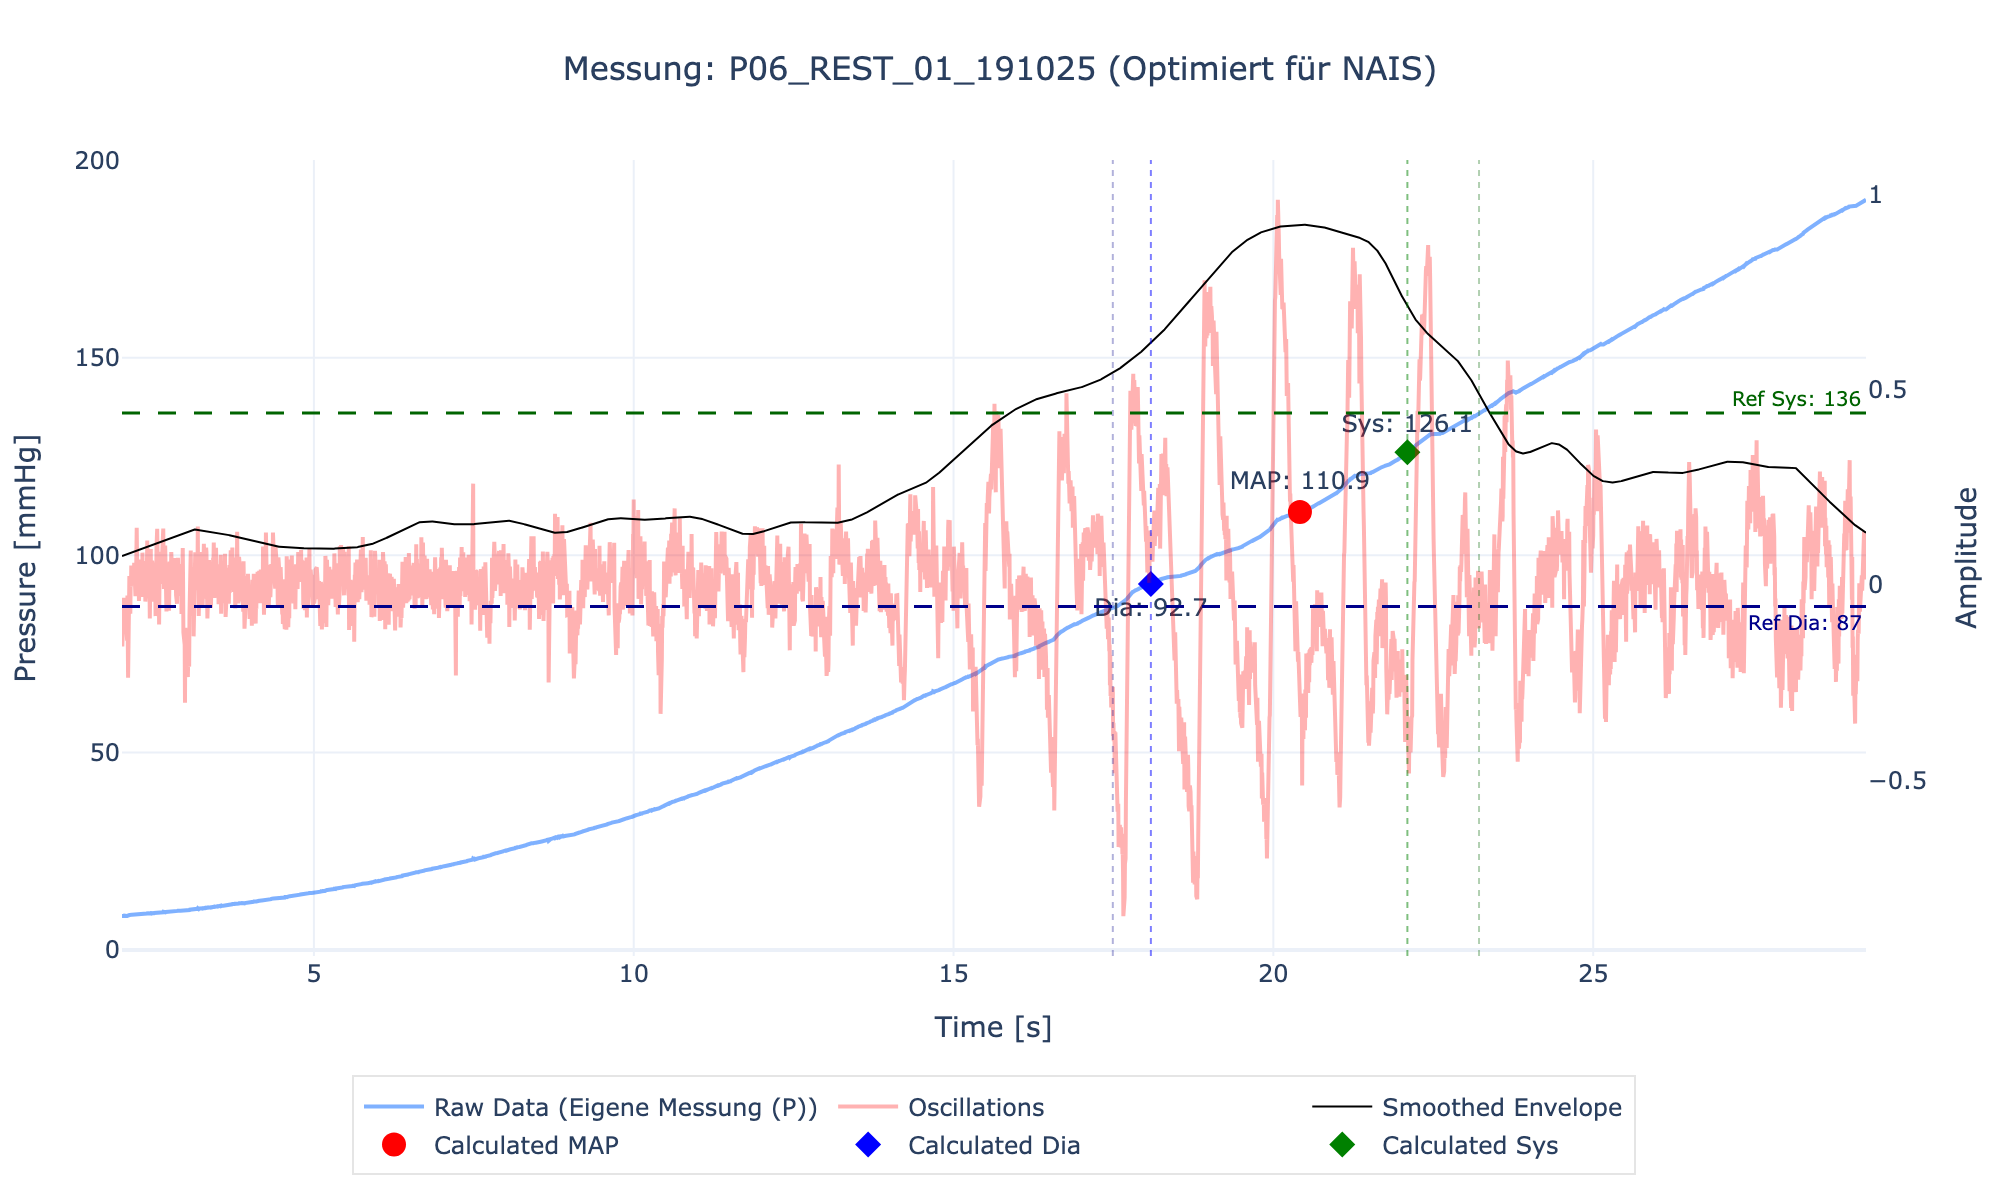
\includegraphics[width=\textwidth]{images/P06_REST_01_191025_nais.png}
        \caption{Optimiert für NAIS}
    \end{subfigure}
    \caption{Einzelauswertung der Messung P06\_REST\_01\_191025 mit verschiedenen Parametersätzen.}
\end{figure}
\newpage

\subsection*{Messung: P07\_ACTIV\_01\_191025}
\begin{figure}[H]
    \centering
    \begin{subfigure}[b]{0.8\textwidth}
        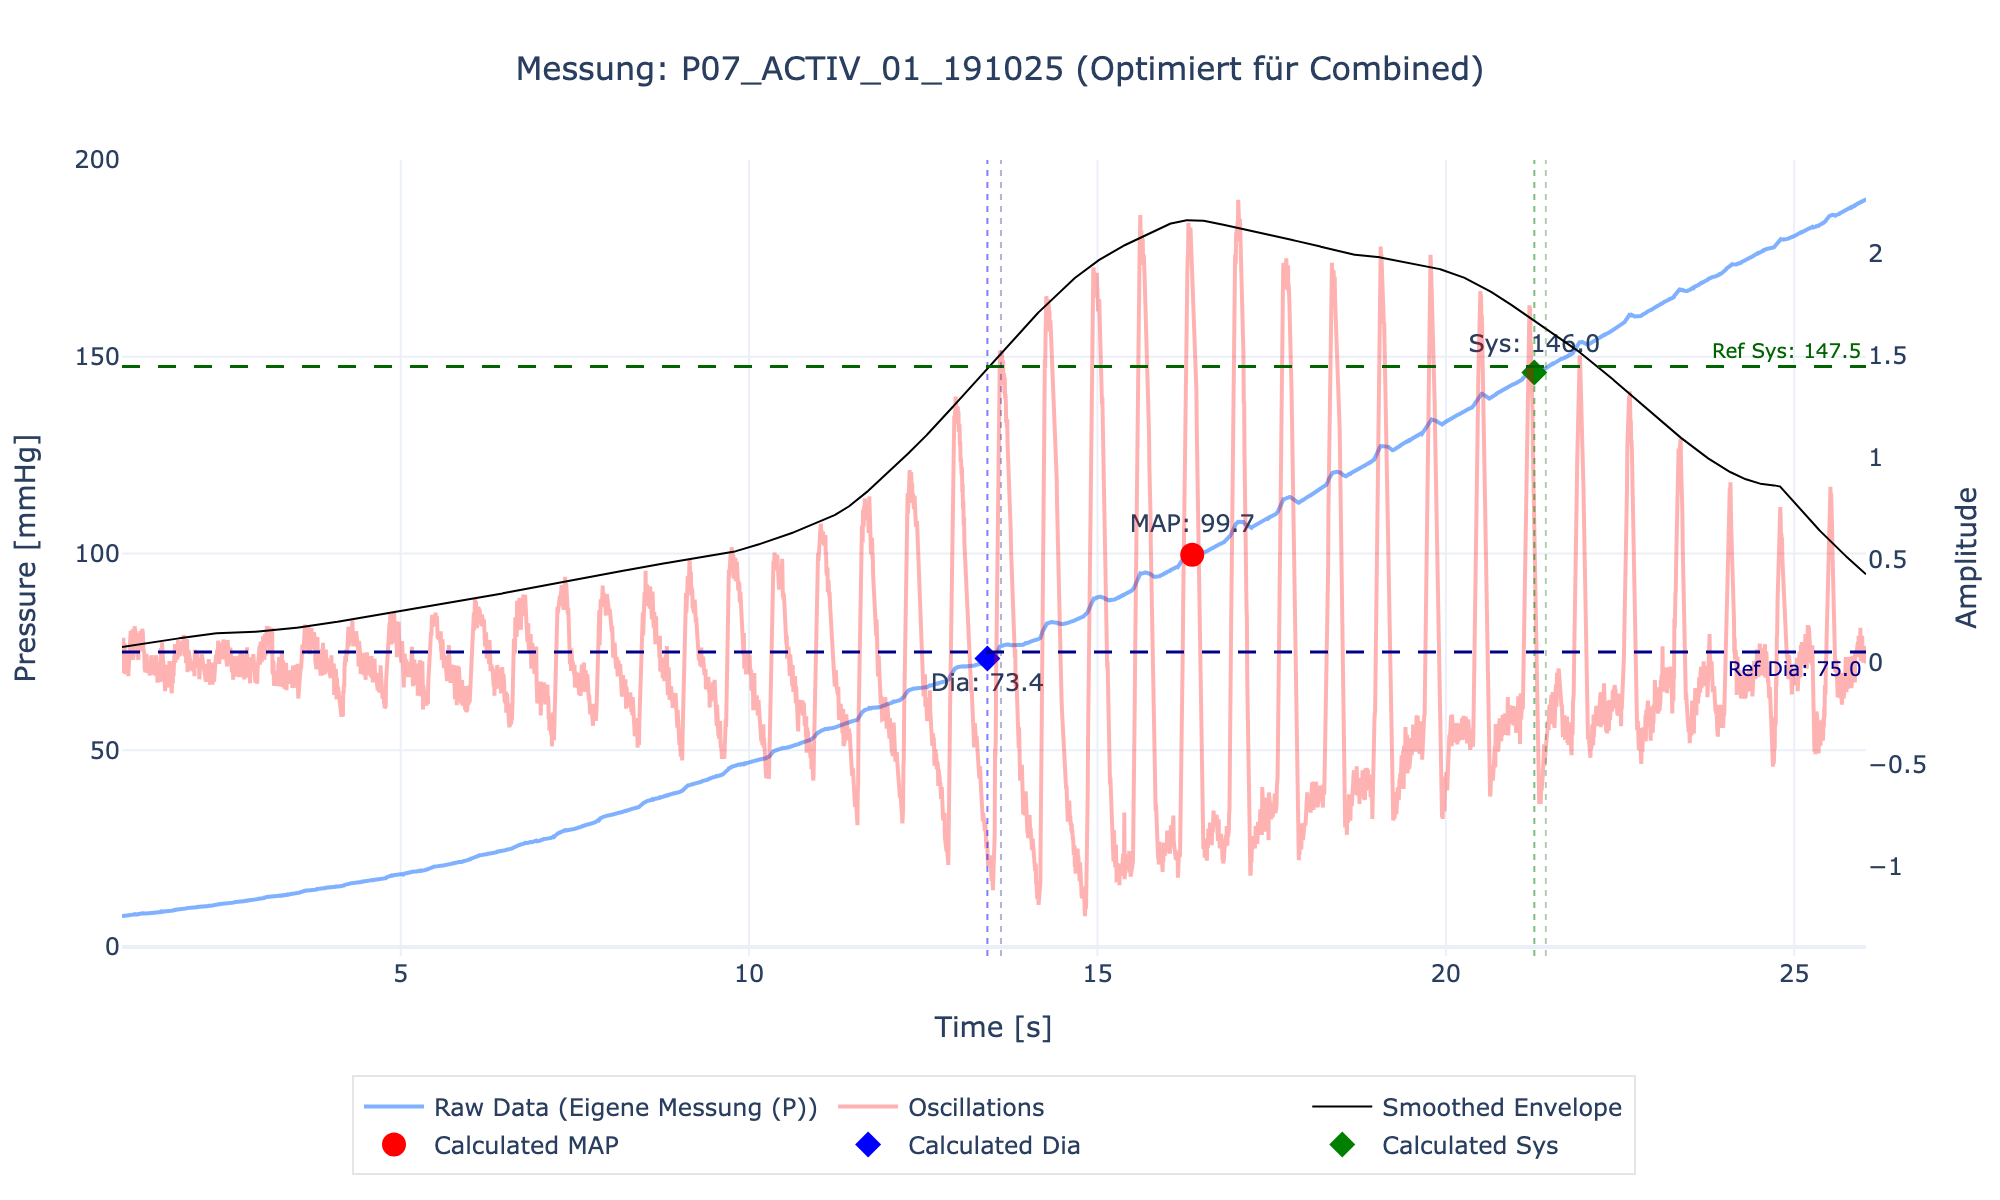
\includegraphics[width=\textwidth]{images/P07_ACTIV_01_191025_combined.png}
        \caption{Optimiert für Beurer und NAIS (Kombiniert)}
    \end{subfigure} \\
    \begin{subfigure}[b]{0.48\textwidth}
        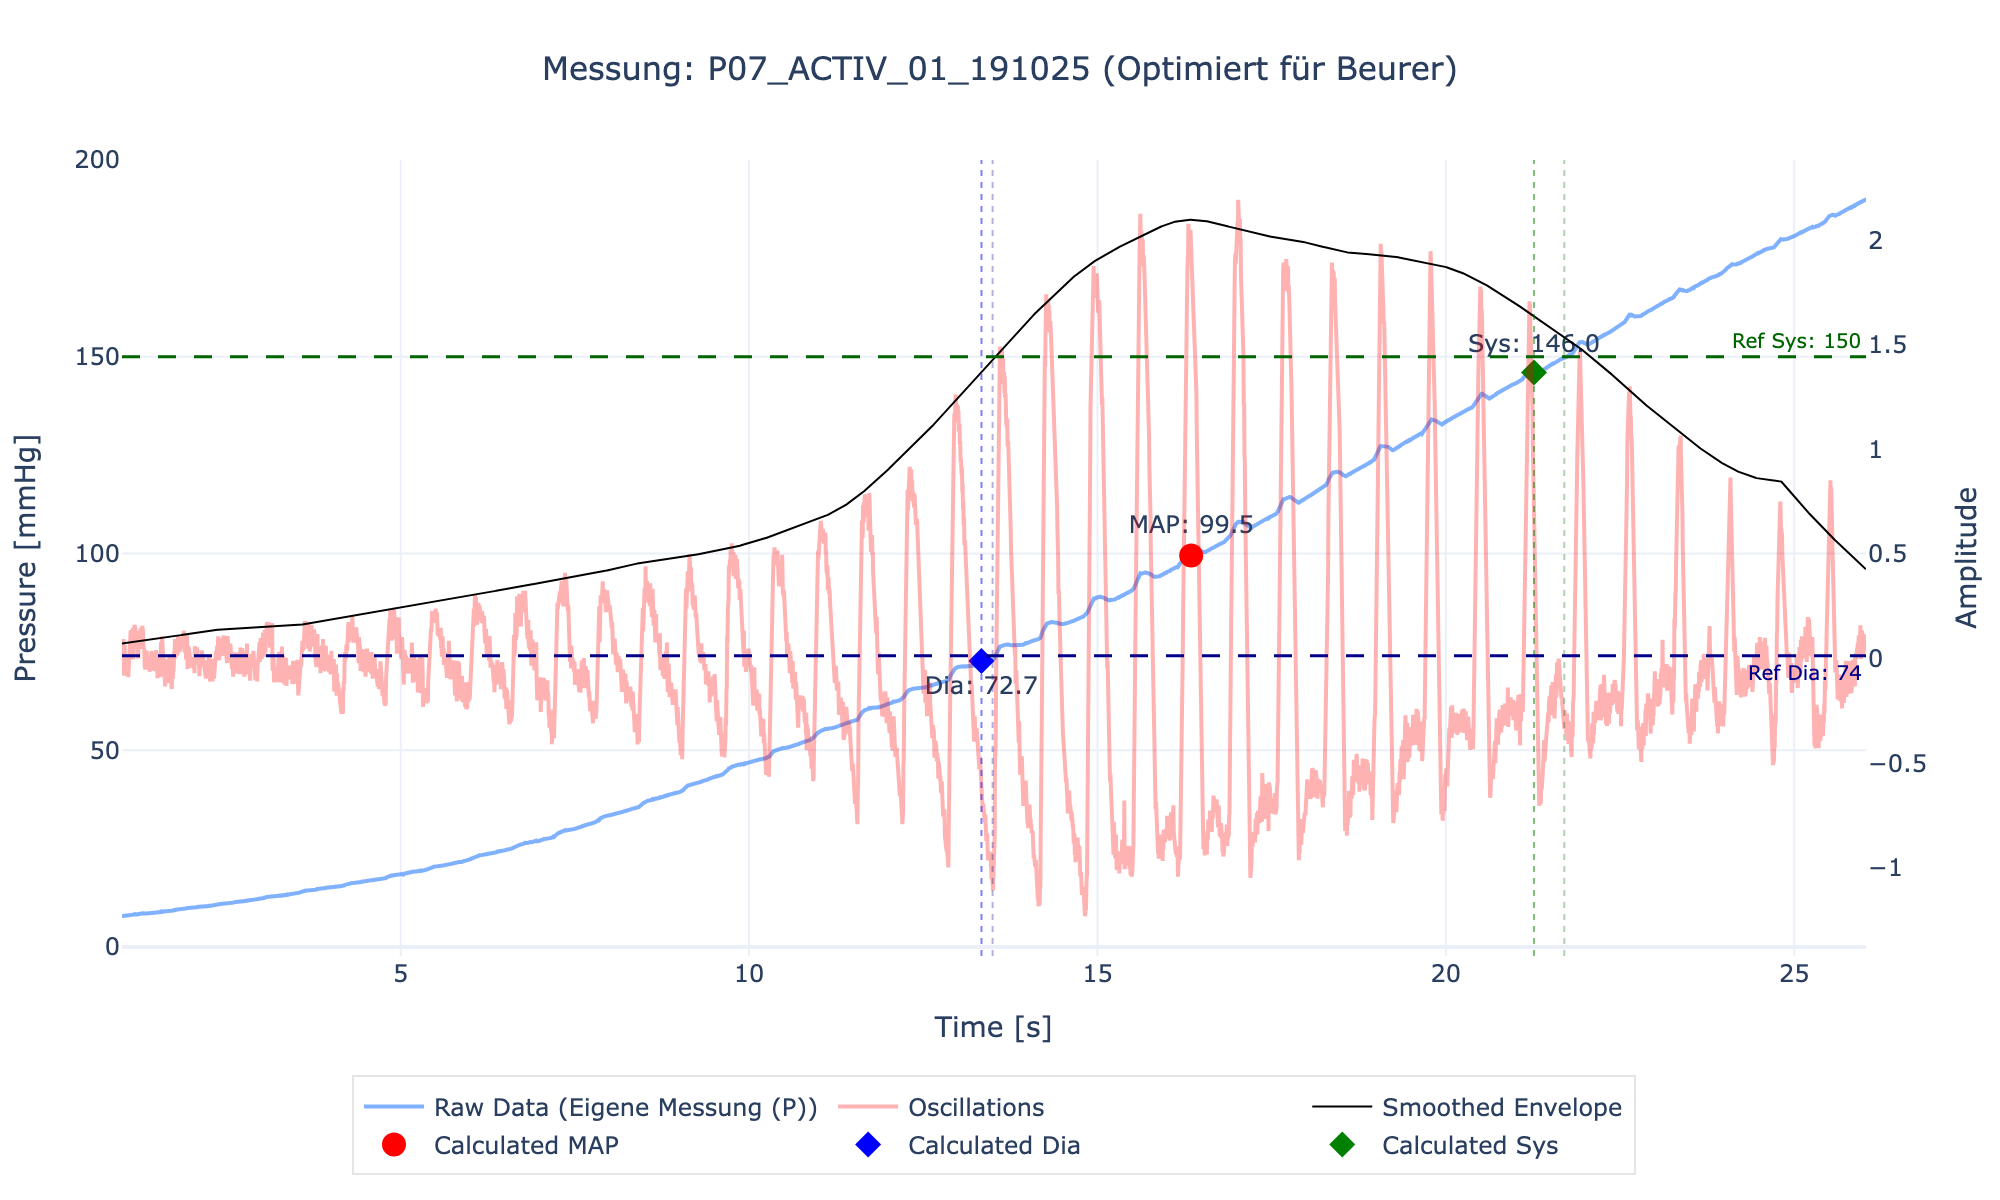
\includegraphics[width=\textwidth]{images/P07_ACTIV_01_191025_beurer.png}
        \caption{Optimiert für Beurer}
    \end{subfigure}
    \hfill
    \begin{subfigure}[b]{0.48\textwidth}
        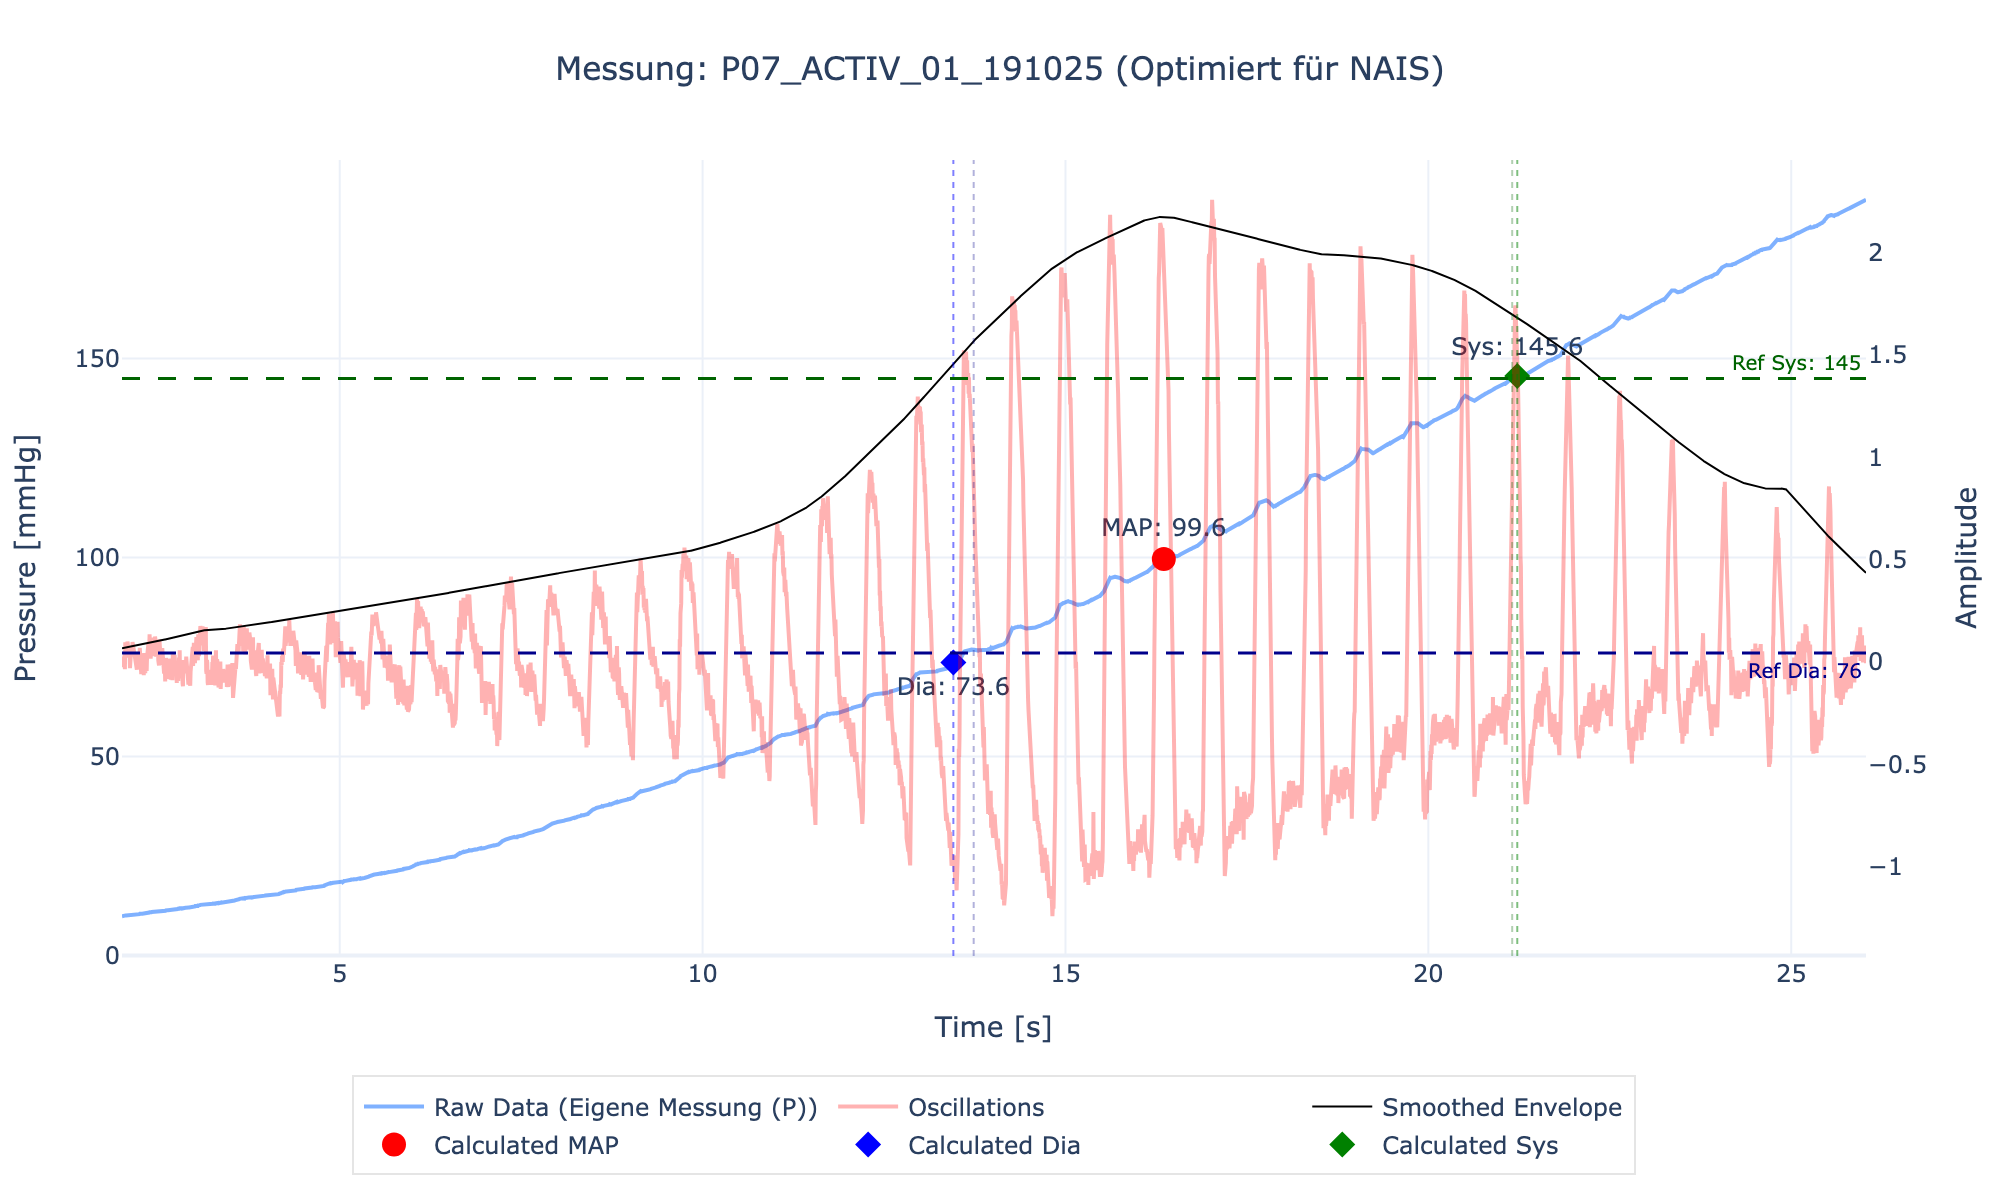
\includegraphics[width=\textwidth]{images/P07_ACTIV_01_191025_nais.png}
        \caption{Optimiert für NAIS}
    \end{subfigure}
    \caption{Einzelauswertung der Messung P07\_ACTIV\_01\_191025 mit verschiedenen Parametersätzen.}
\end{figure}
\newpage

\subsection*{Messung: P07\_REST\_01\_191025}
\begin{figure}[H]
    \centering
    \begin{subfigure}[b]{0.8\textwidth}
        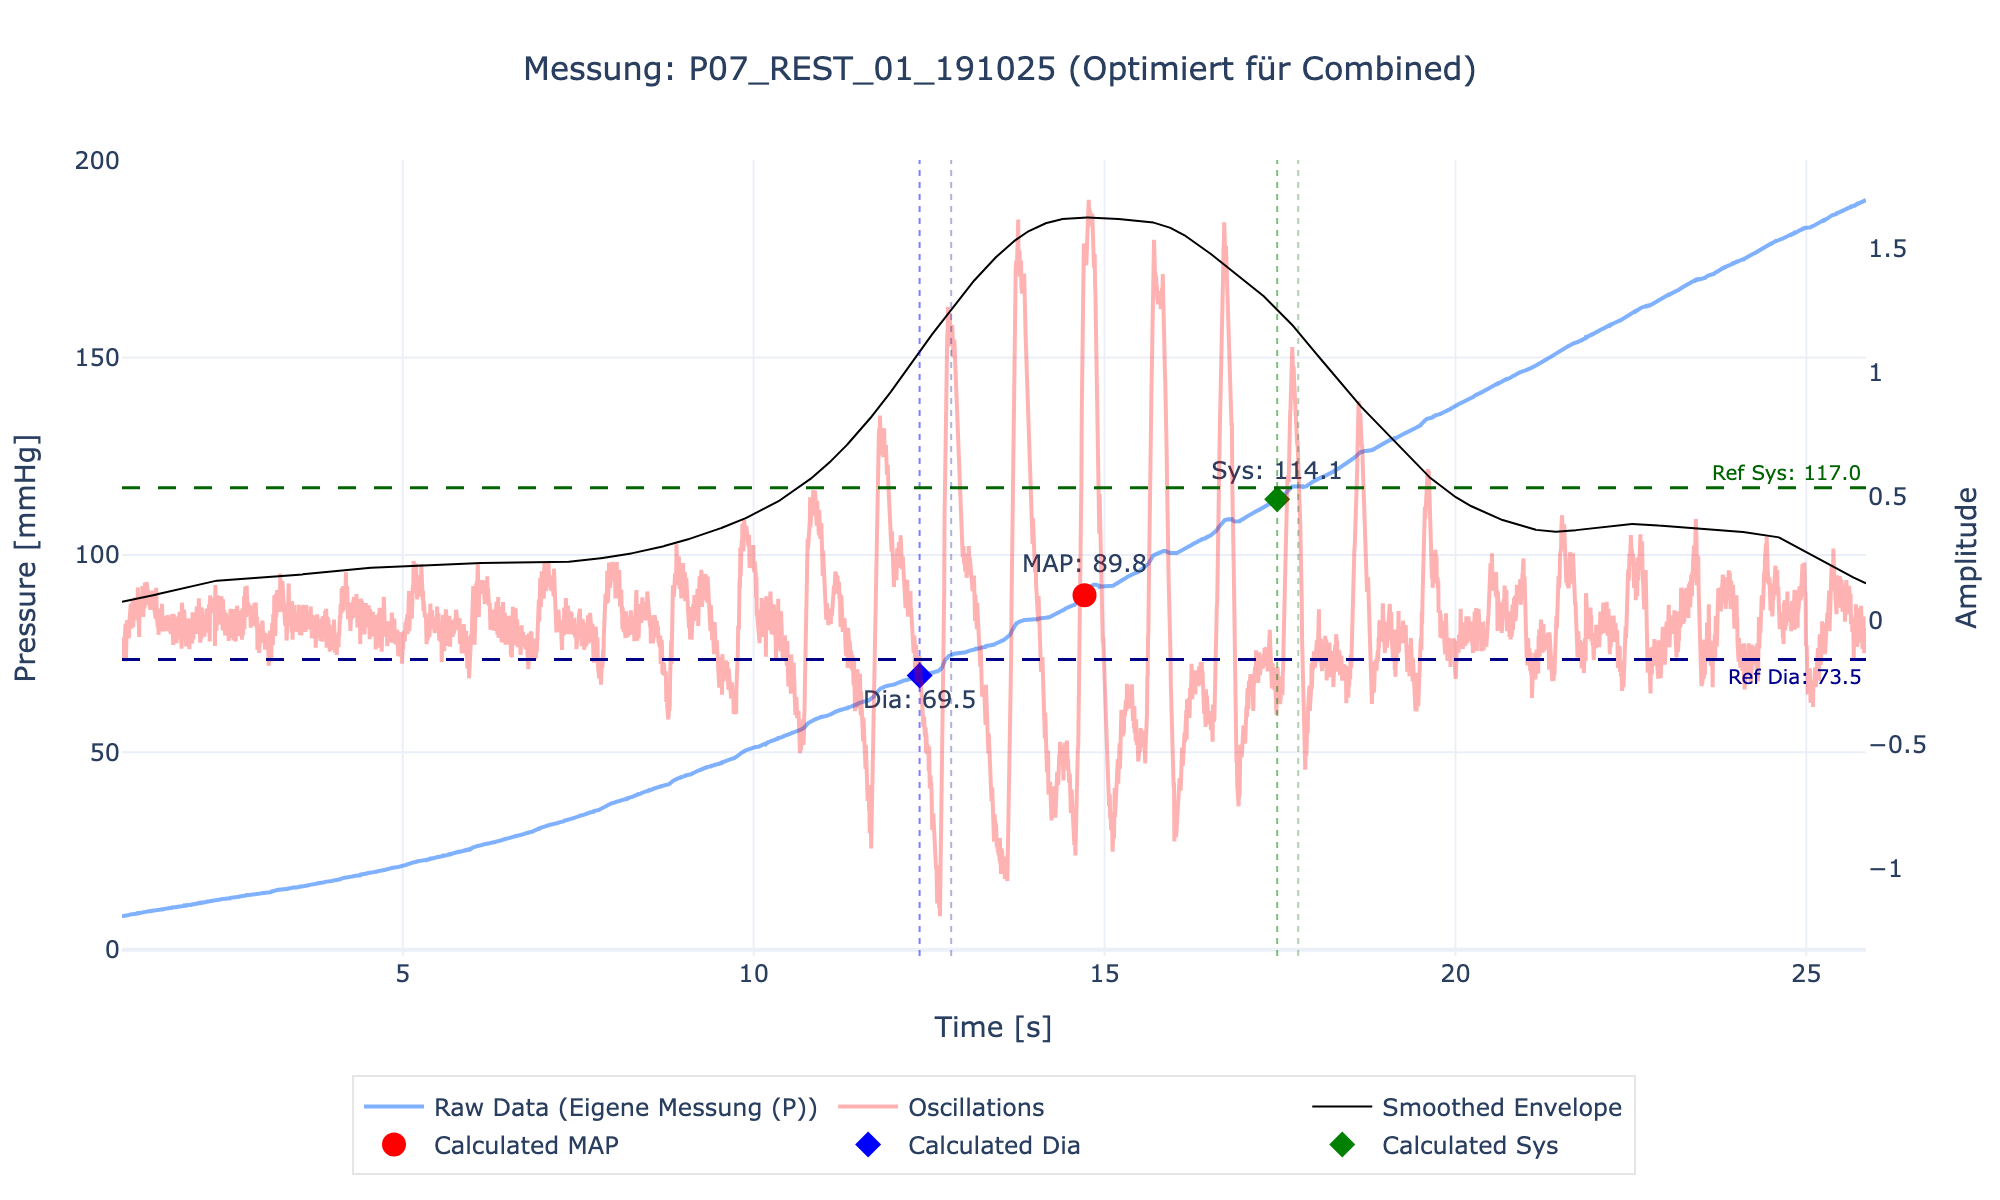
\includegraphics[width=\textwidth]{images/P07_REST_01_191025_combined.png}
        \caption{Optimiert für Beurer und NAIS (Kombiniert)}
    \end{subfigure} \\
    \begin{subfigure}[b]{0.48\textwidth}
        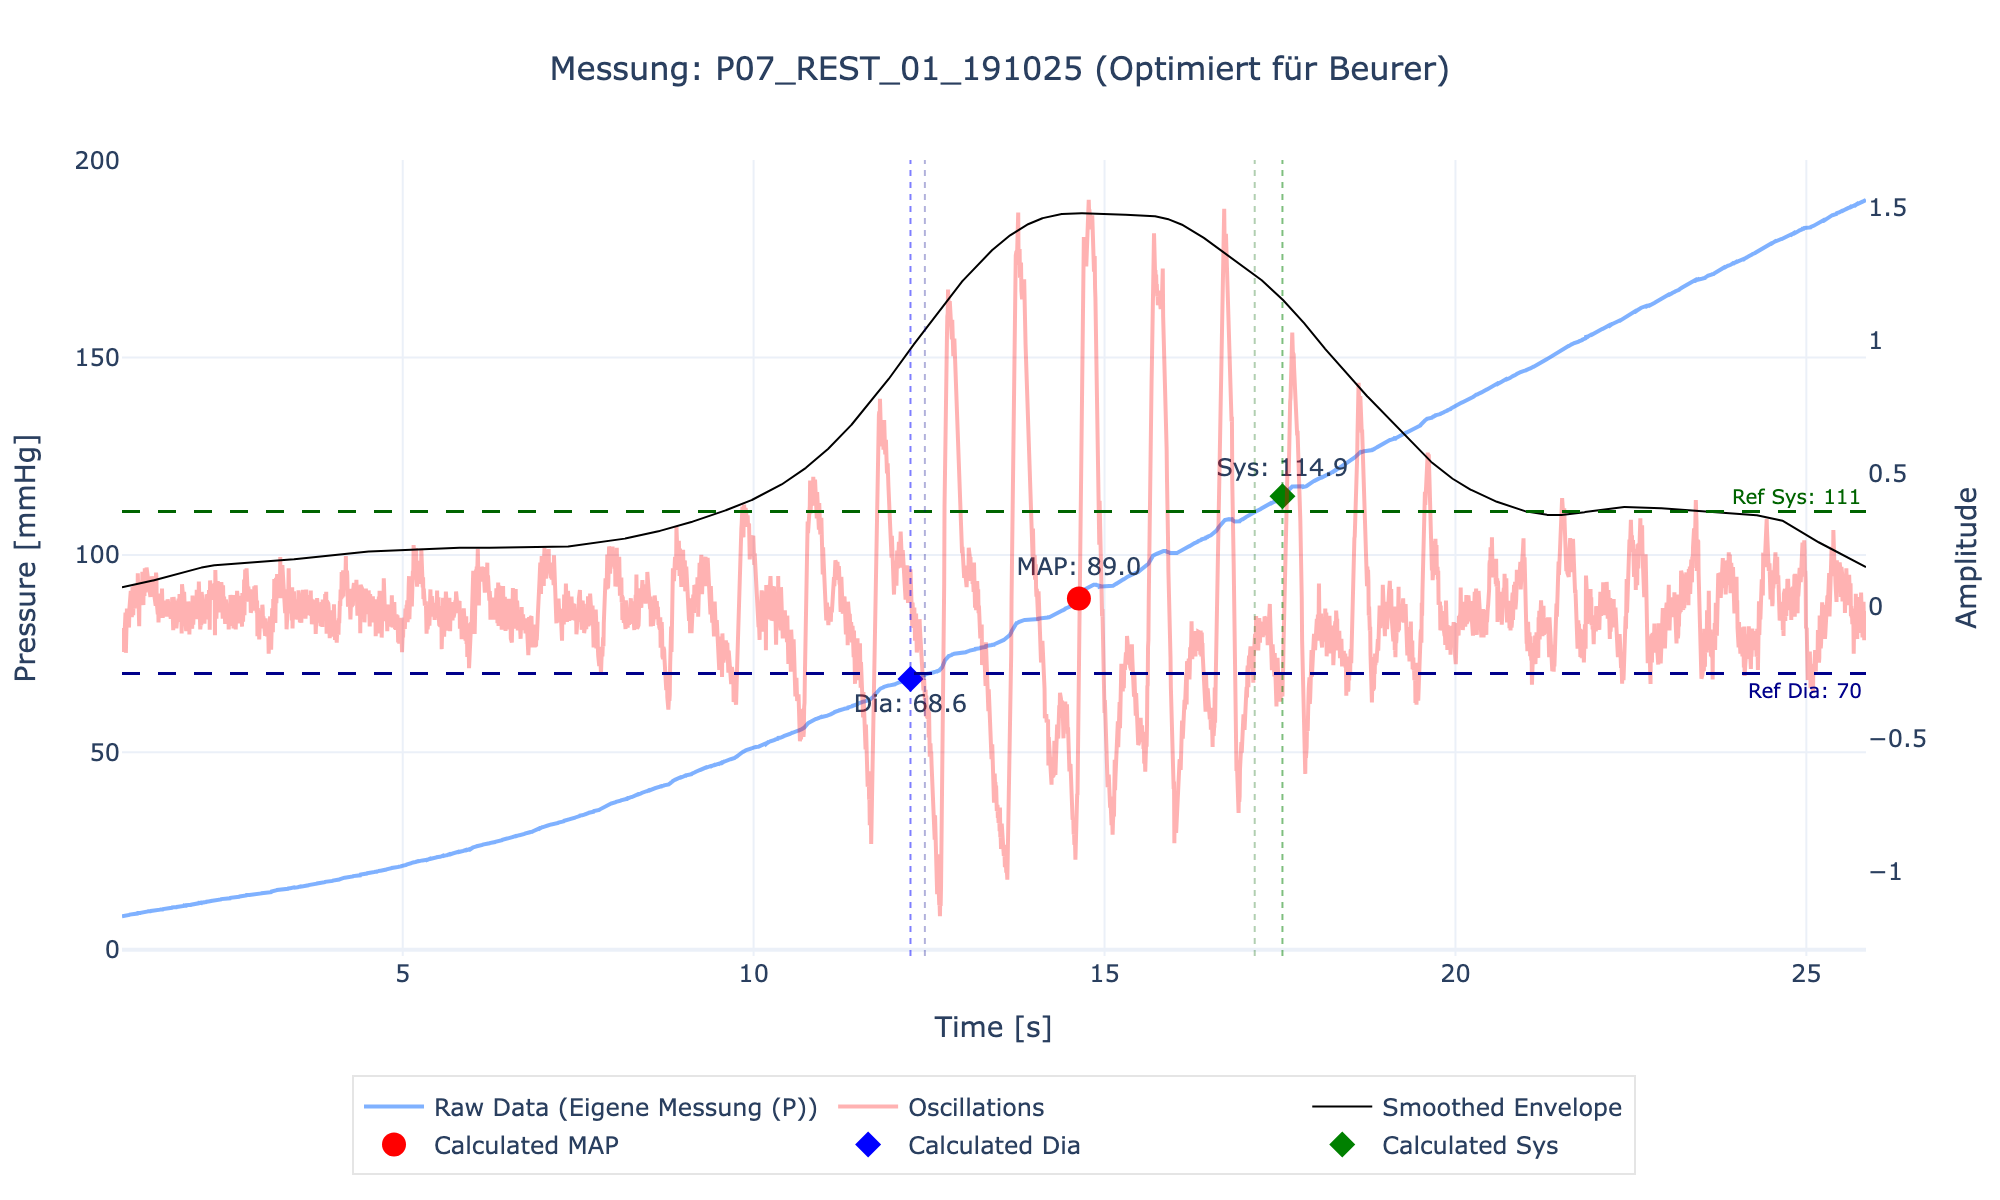
\includegraphics[width=\textwidth]{images/P07_REST_01_191025_beurer.png}
        \caption{Optimiert für Beurer}
    \end{subfigure}
    \hfill
    \begin{subfigure}[b]{0.48\textwidth}
        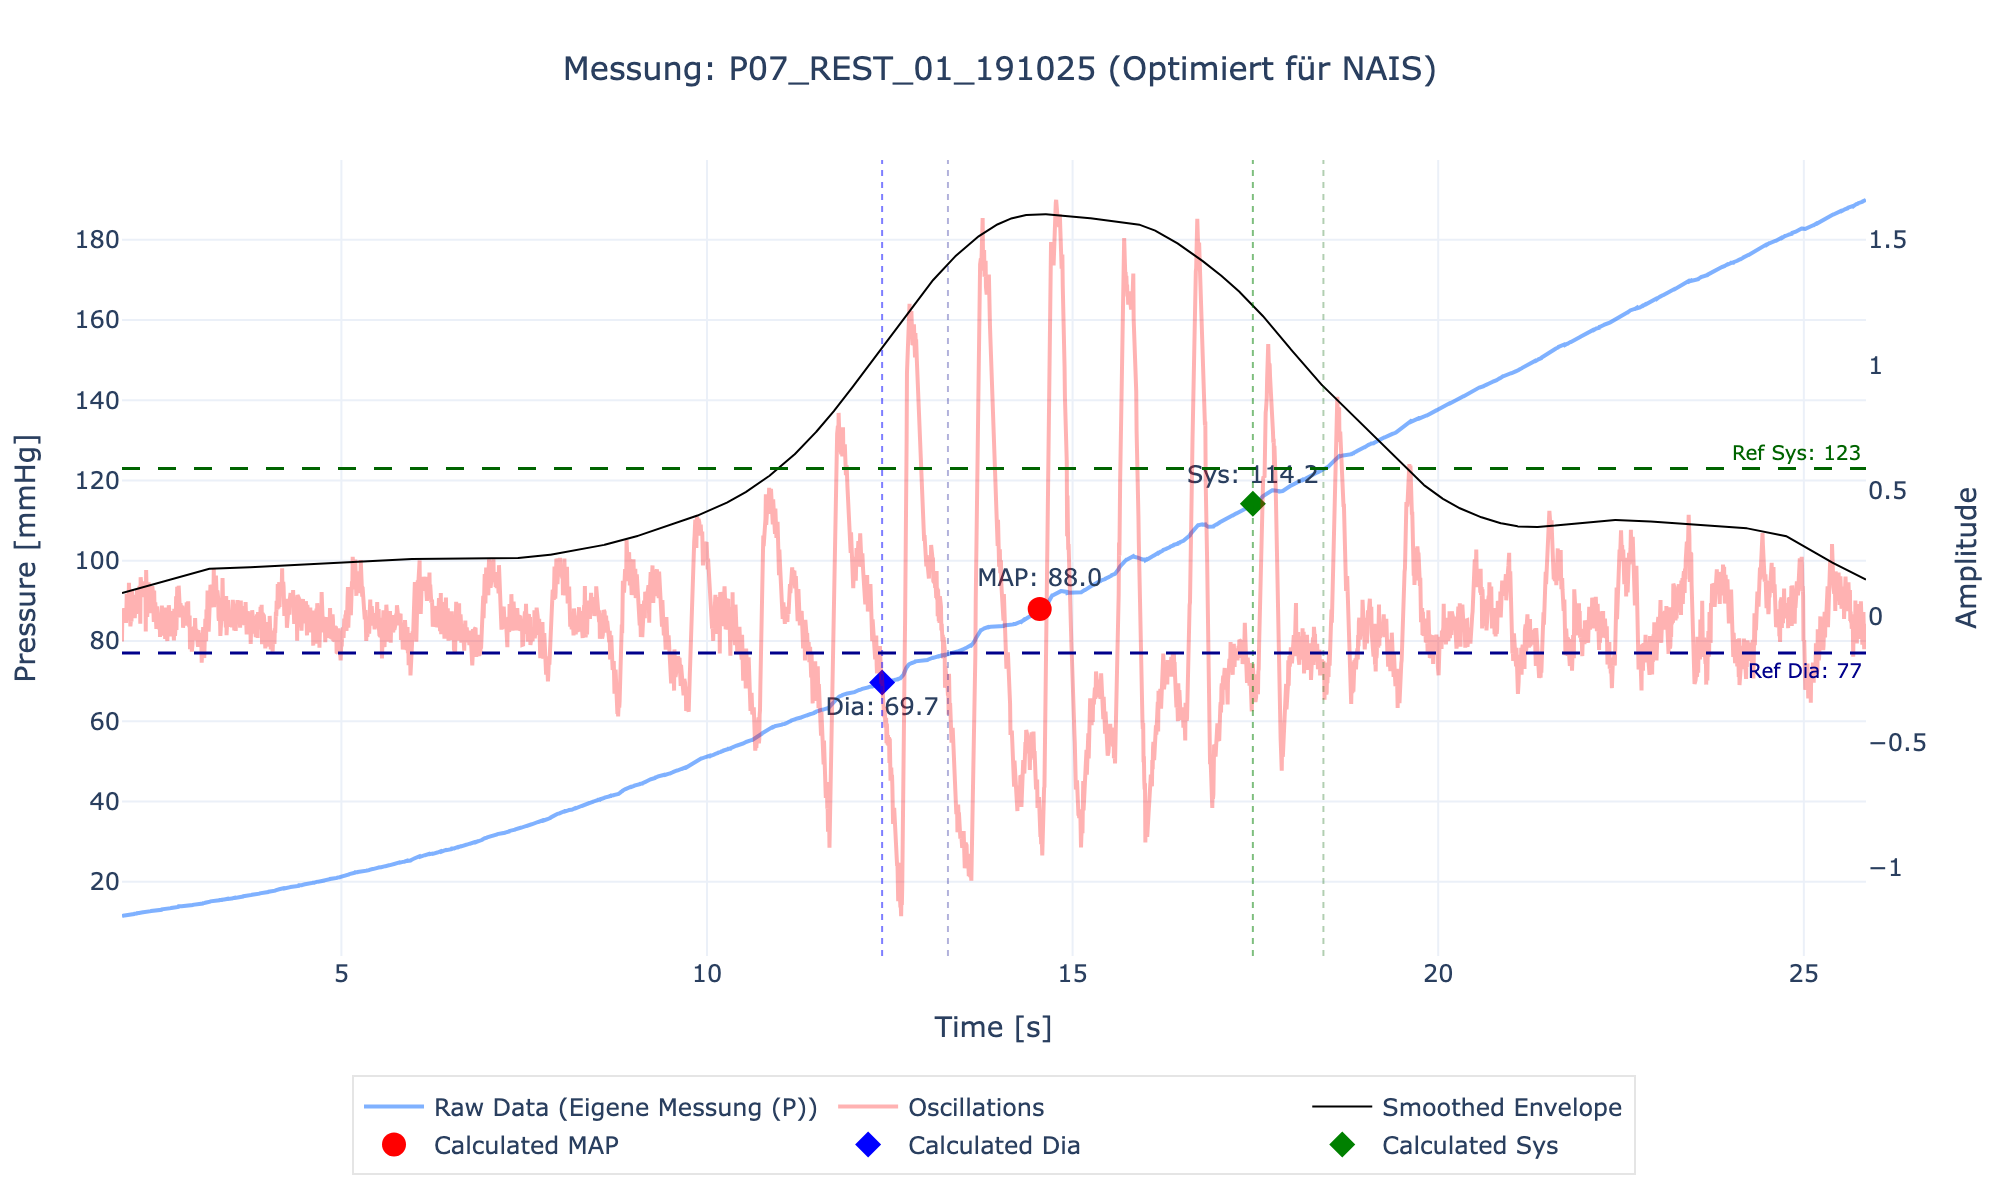
\includegraphics[width=\textwidth]{images/P07_REST_01_191025_nais.png}
        \caption{Optimiert für NAIS}
    \end{subfigure}
    \caption{Einzelauswertung der Messung P07\_REST\_01\_191025 mit verschiedenen Parametersätzen.}
\end{figure}
\newpage

\subsection*{Messung: P08\_ACTIV\_01\_201025}
\begin{figure}[H]
    \centering
    \begin{subfigure}[b]{0.8\textwidth}
        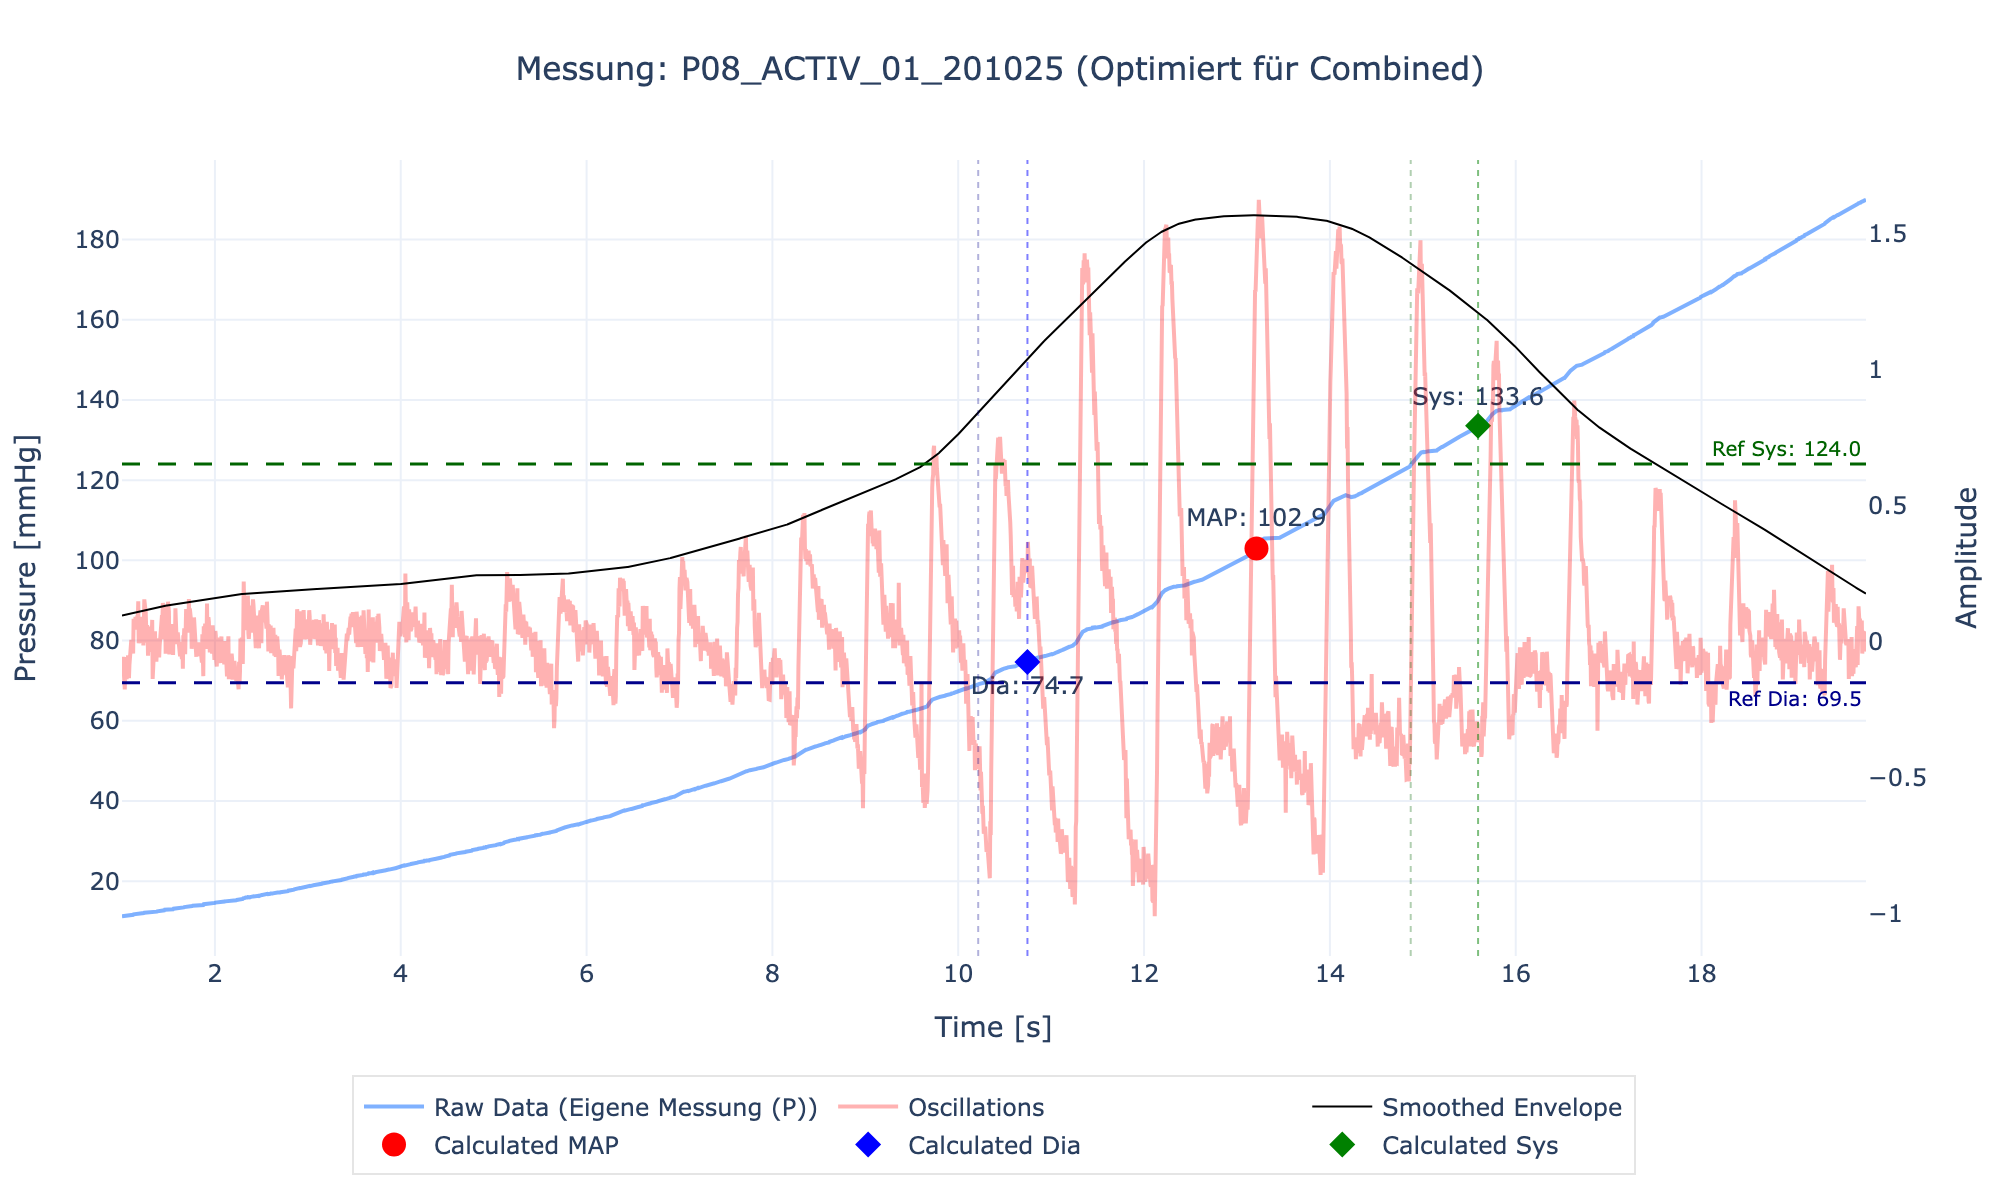
\includegraphics[width=\textwidth]{images/P08_ACTIV_01_201025_combined.png}
        \caption{Optimiert für Beurer und NAIS (Kombiniert)}
    \end{subfigure} \\
    \begin{subfigure}[b]{0.48\textwidth}
        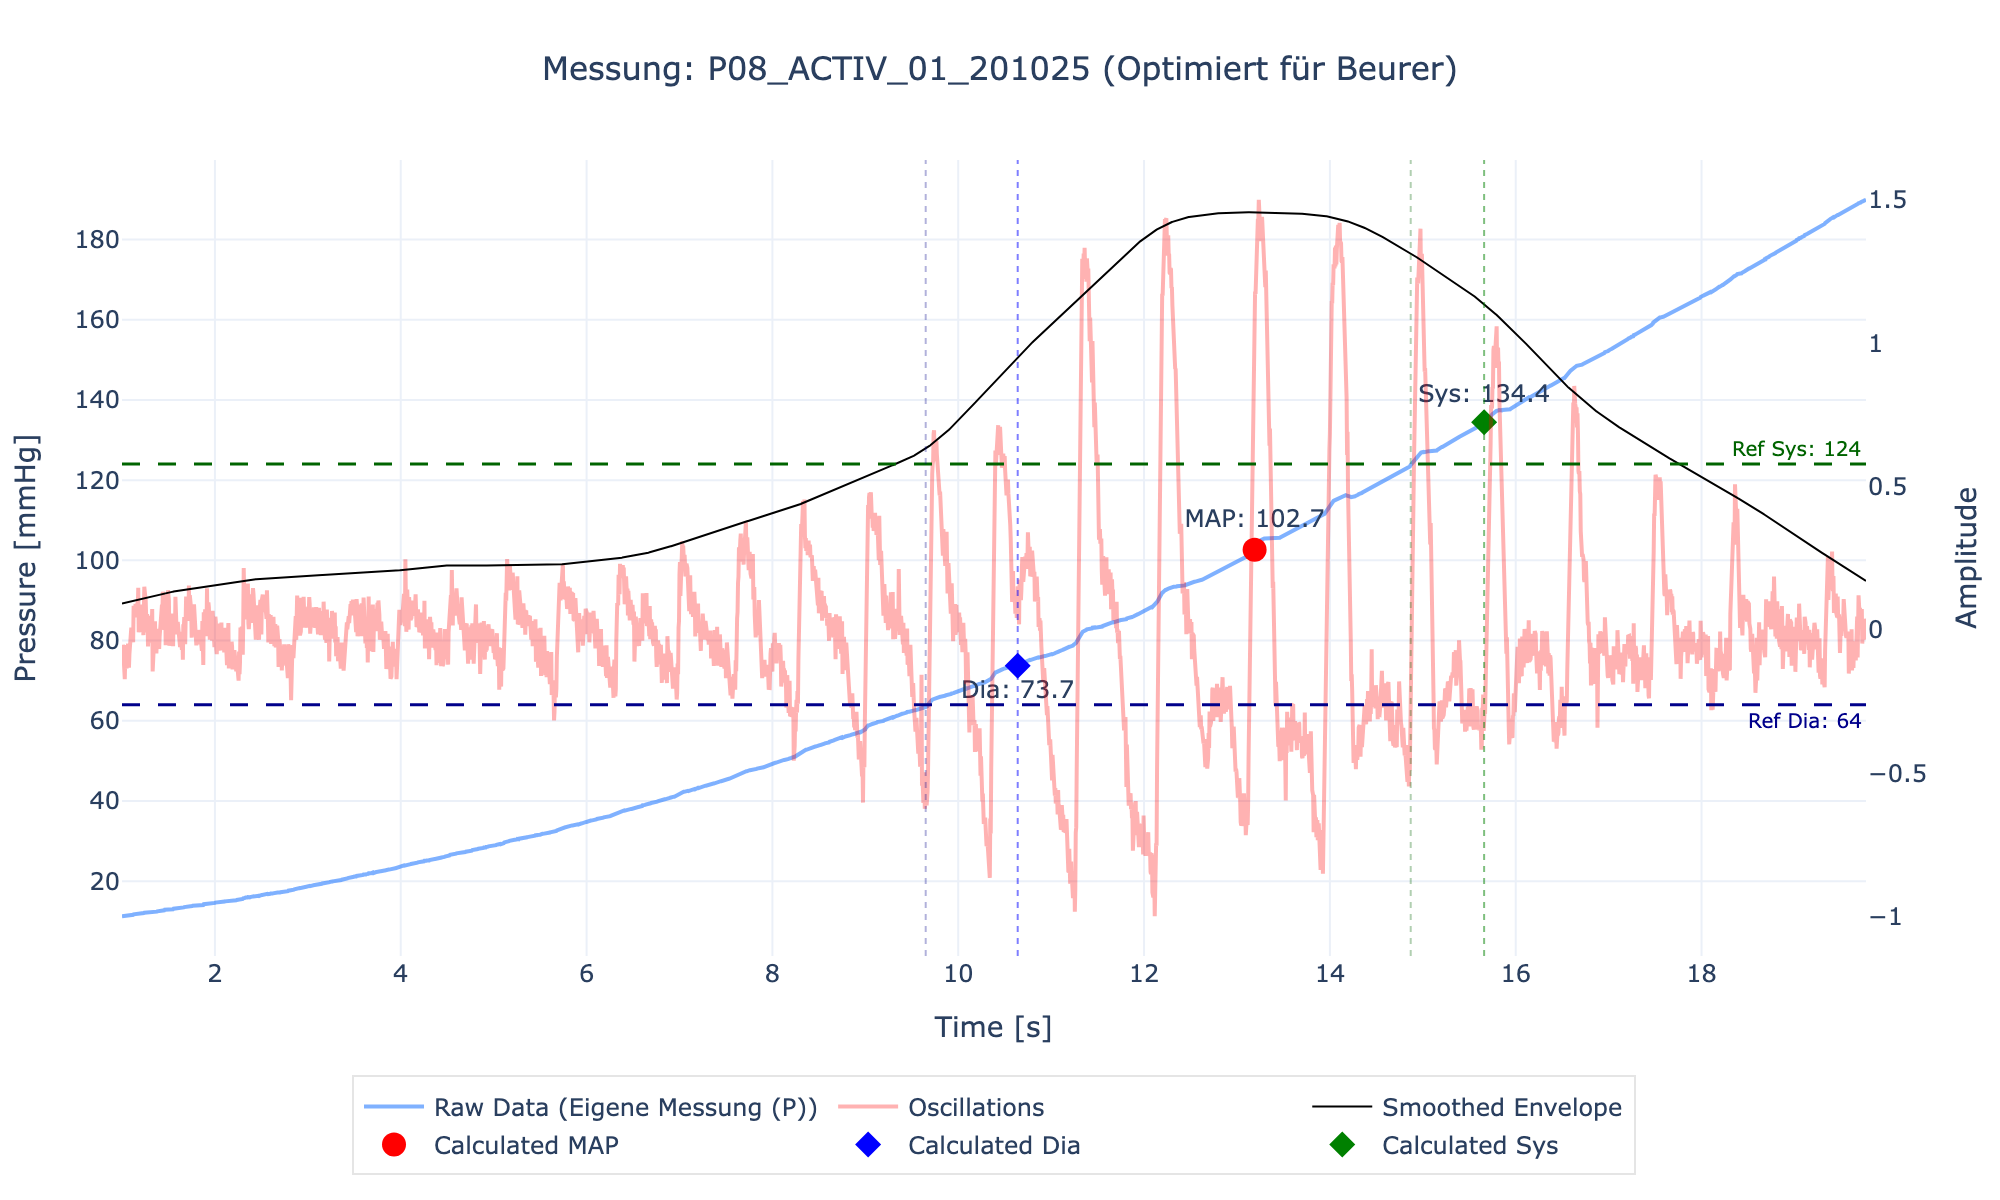
\includegraphics[width=\textwidth]{images/P08_ACTIV_01_201025_beurer.png}
        \caption{Optimiert für Beurer}
    \end{subfigure}
    \hfill
    \begin{subfigure}[b]{0.48\textwidth}
        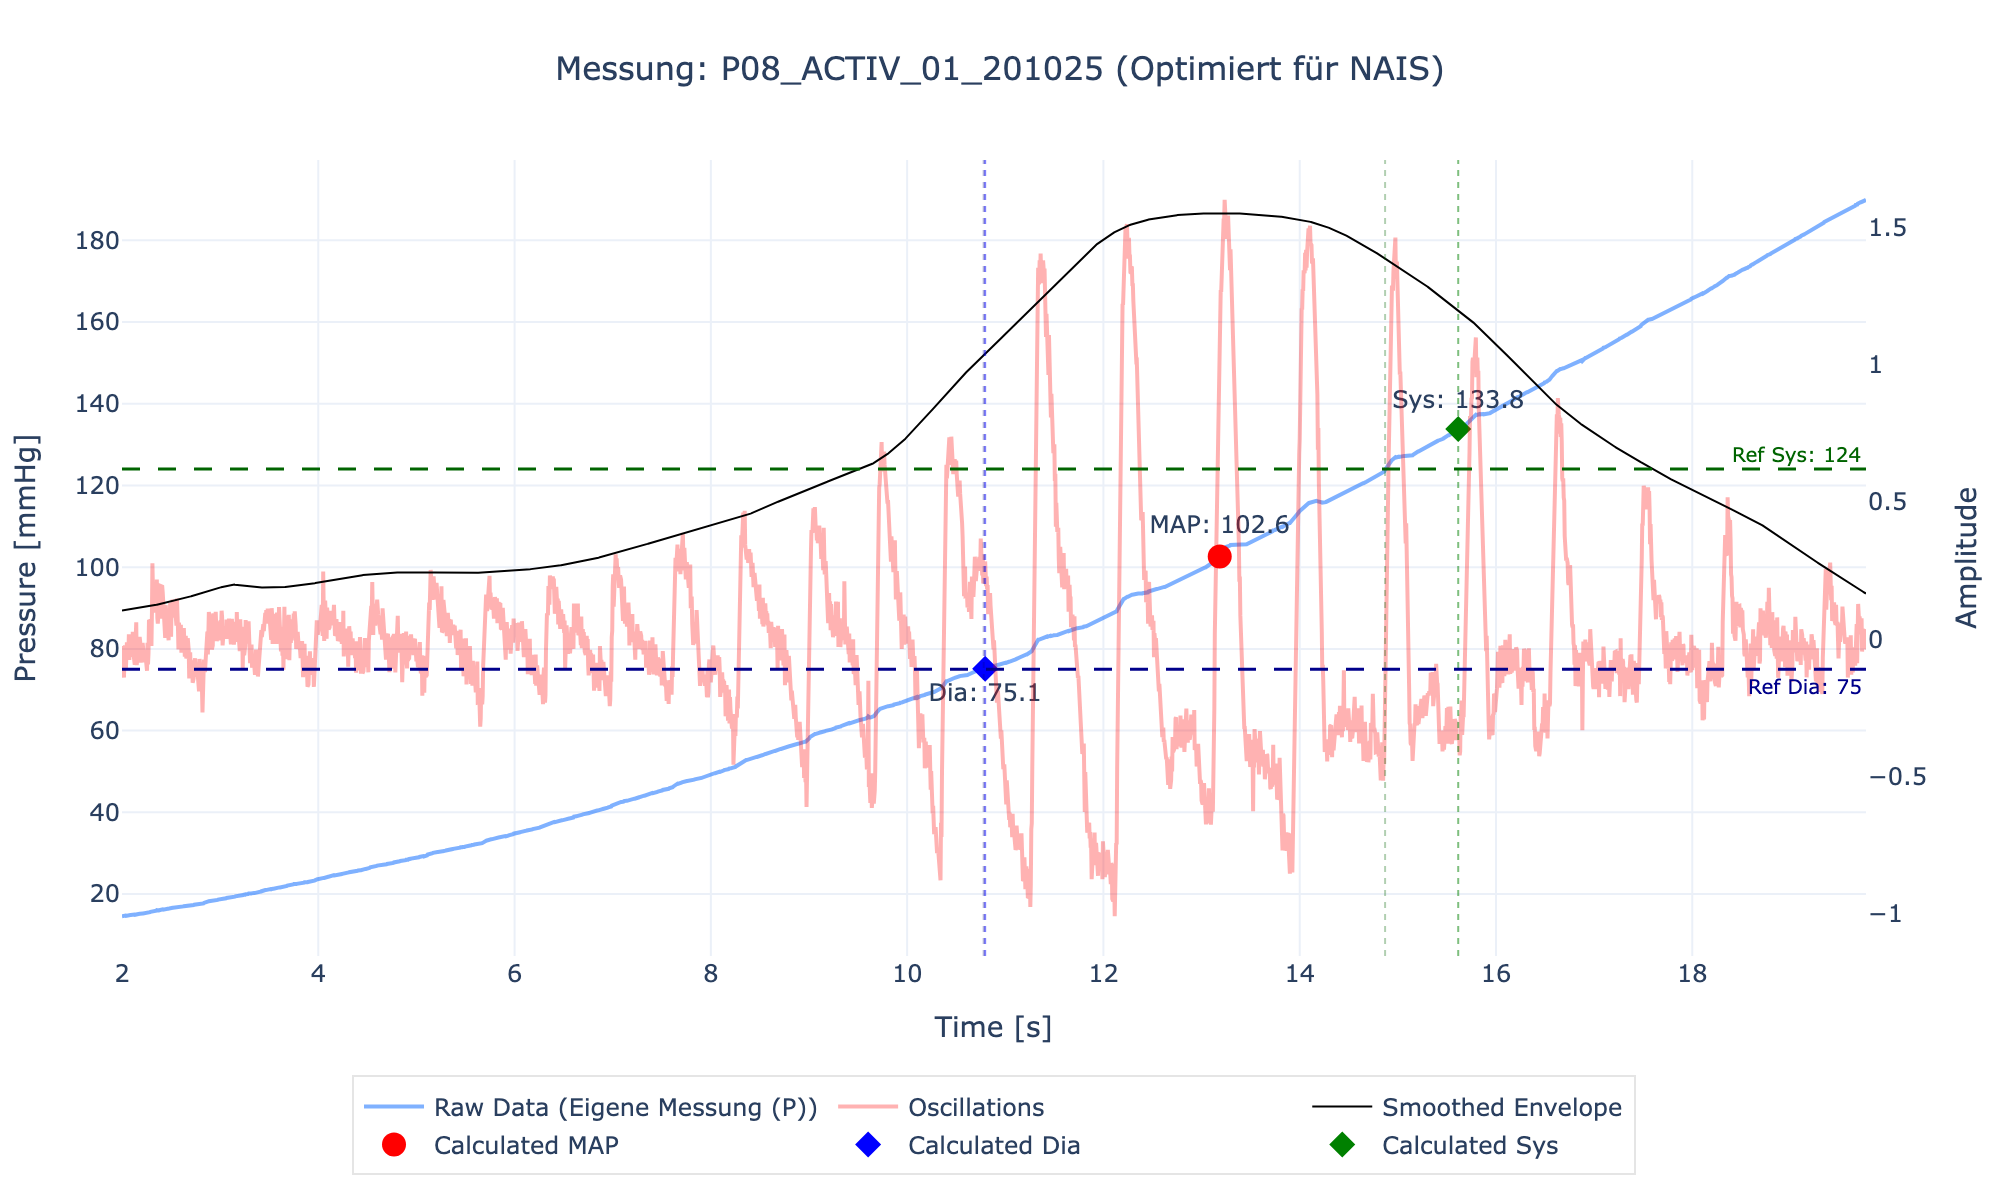
\includegraphics[width=\textwidth]{images/P08_ACTIV_01_201025_nais.png}
        \caption{Optimiert für NAIS}
    \end{subfigure}
    \caption{Einzelauswertung der Messung P08\_ACTIV\_01\_201025 mit verschiedenen Parametersätzen.}
\end{figure}
\newpage

\subsection*{Messung: P08\_REST\_01\_201025}
\begin{figure}[H]
    \centering
    \begin{subfigure}[b]{0.8\textwidth}
        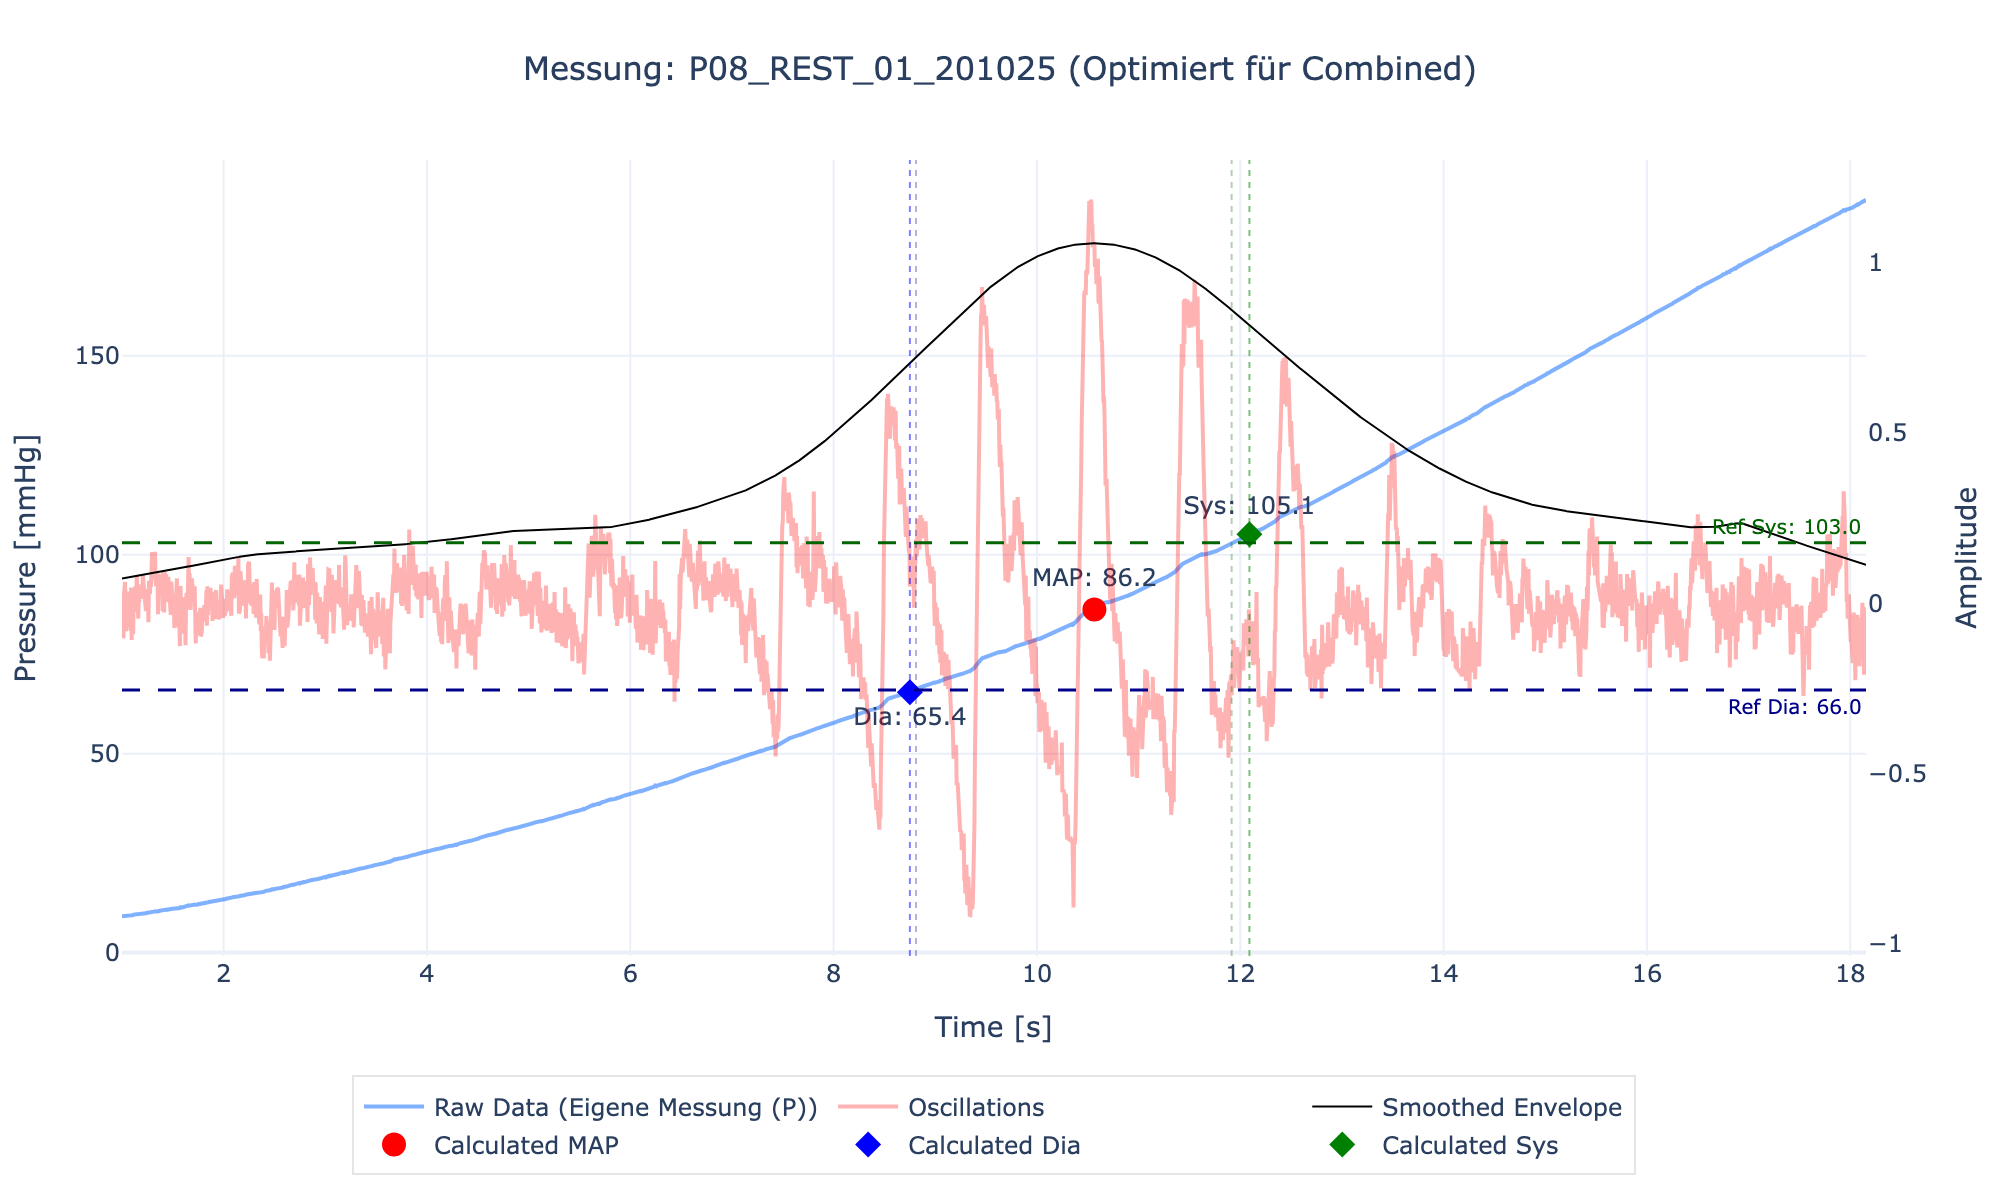
\includegraphics[width=\textwidth]{images/P08_REST_01_201025_combined.png}
        \caption{Optimiert für Beurer und NAIS (Kombiniert)}
    \end{subfigure} \\
    \begin{subfigure}[b]{0.48\textwidth}
        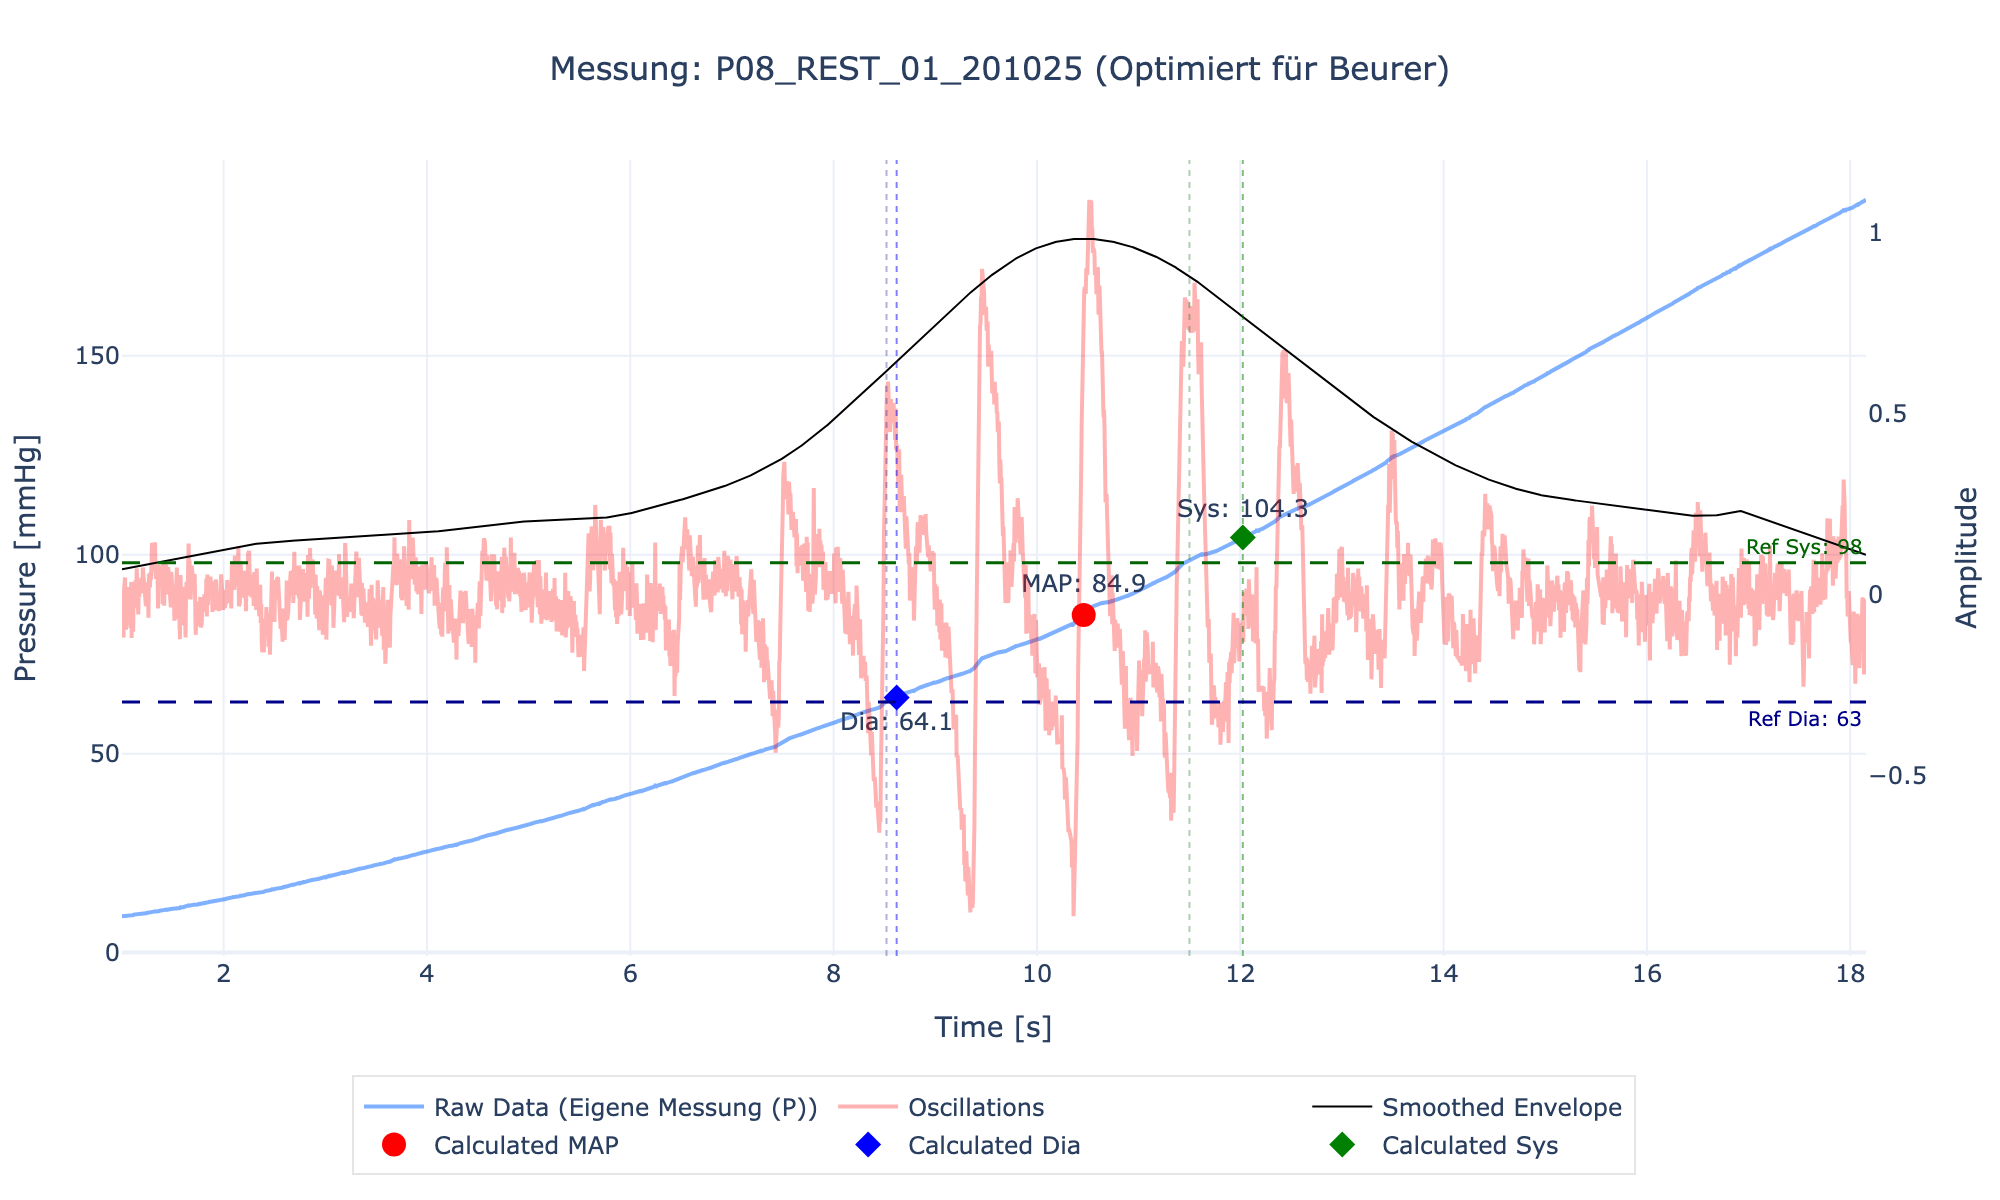
\includegraphics[width=\textwidth]{images/P08_REST_01_201025_beurer.png}
        \caption{Optimiert für Beurer}
    \end{subfigure}
    \hfill
    \begin{subfigure}[b]{0.48\textwidth}
        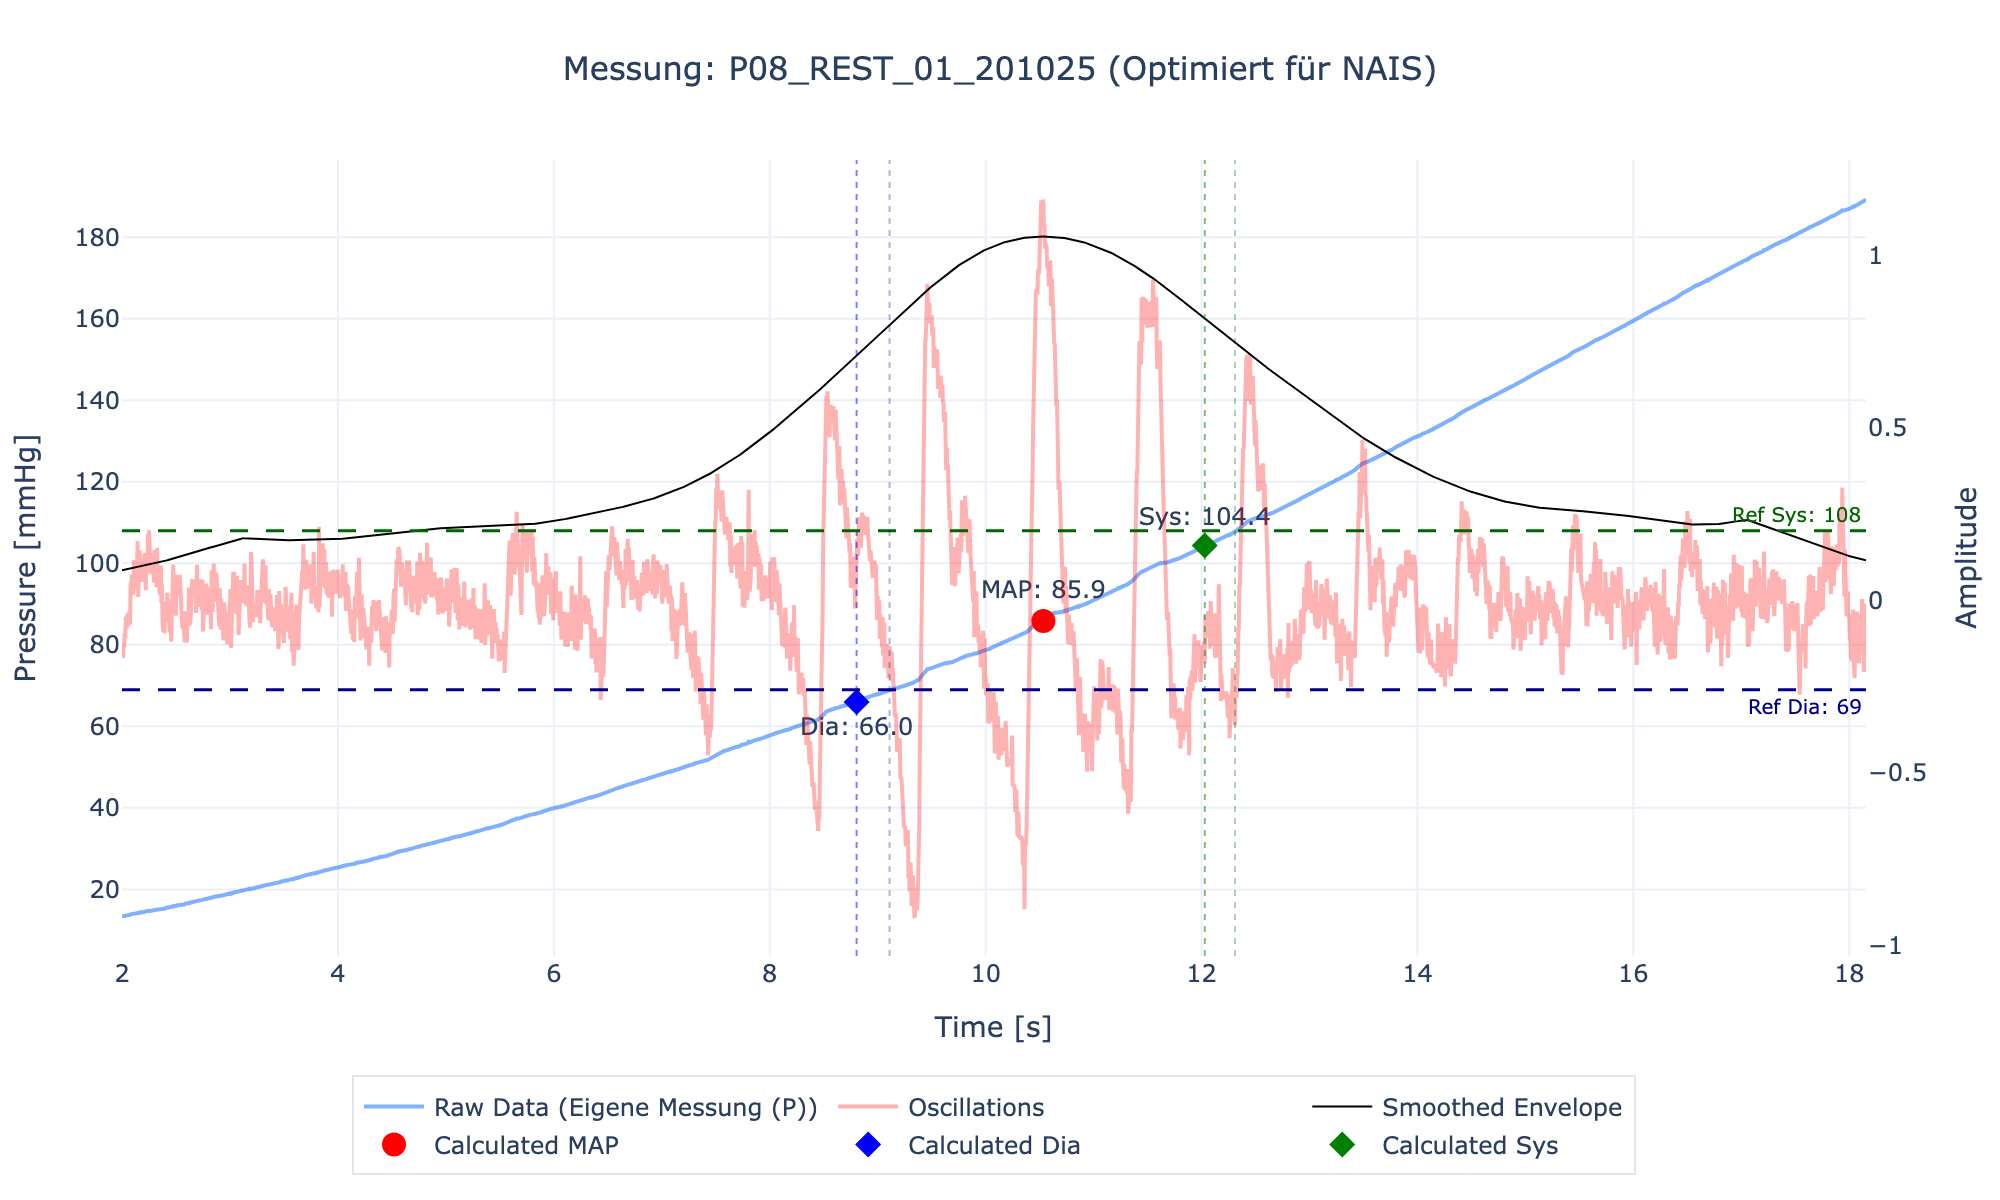
\includegraphics[width=\textwidth]{images/P08_REST_01_201025_nais.png}
        \caption{Optimiert für NAIS}
    \end{subfigure}
    \caption{Einzelauswertung der Messung P08\_REST\_01\_201025 mit verschiedenen Parametersätzen.}
\end{figure}
\newpage

\subsection*{Messung: S001-M001-Rest}
\begin{figure}[H]
    \centering
    \begin{subfigure}[b]{0.8\textwidth}
        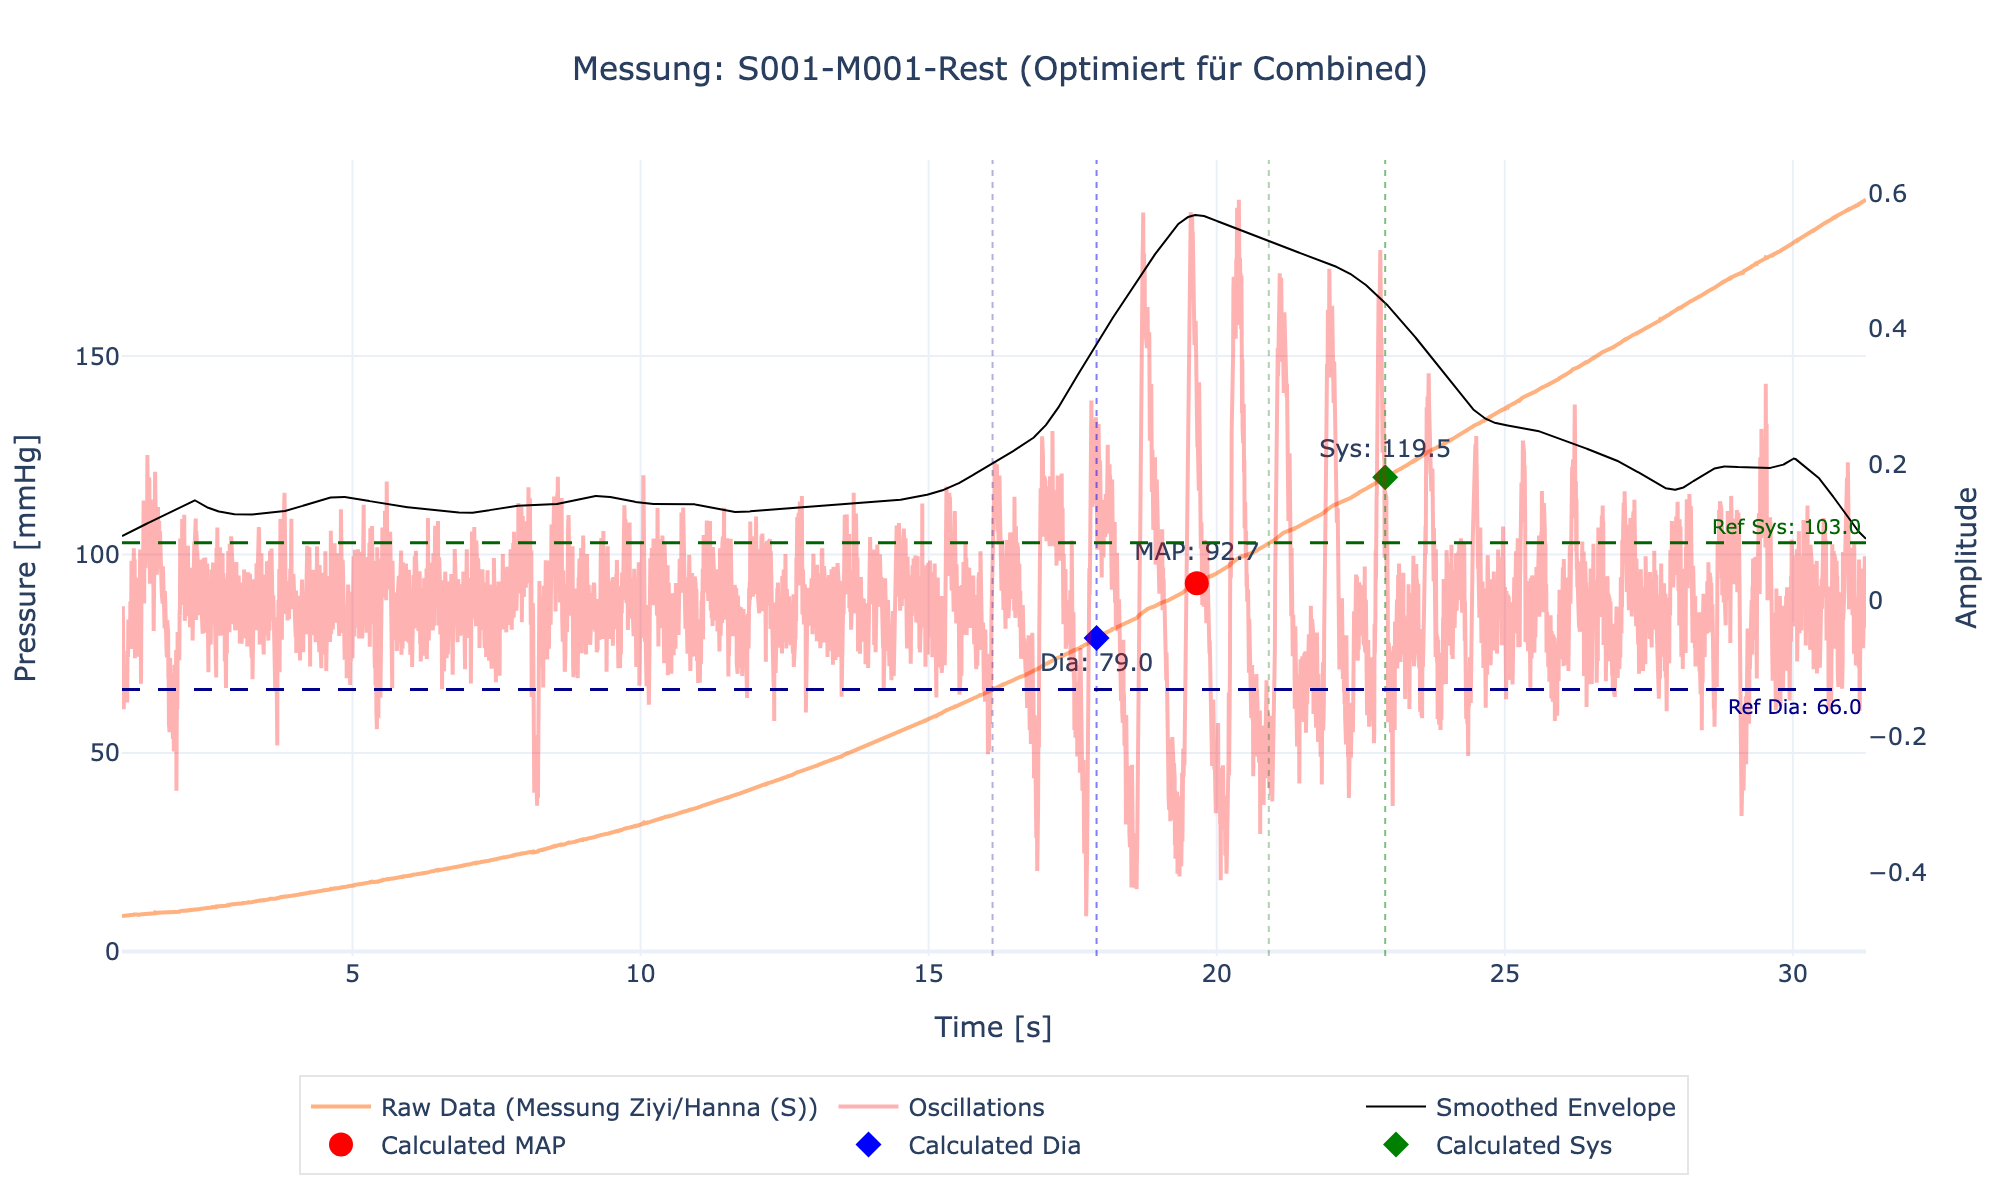
\includegraphics[width=\textwidth]{images/S001-M001-Rest_combined.png}
        \caption{Optimiert für Beurer und NAIS (Kombiniert)}
    \end{subfigure} \\
    \begin{subfigure}[b]{0.48\textwidth}
        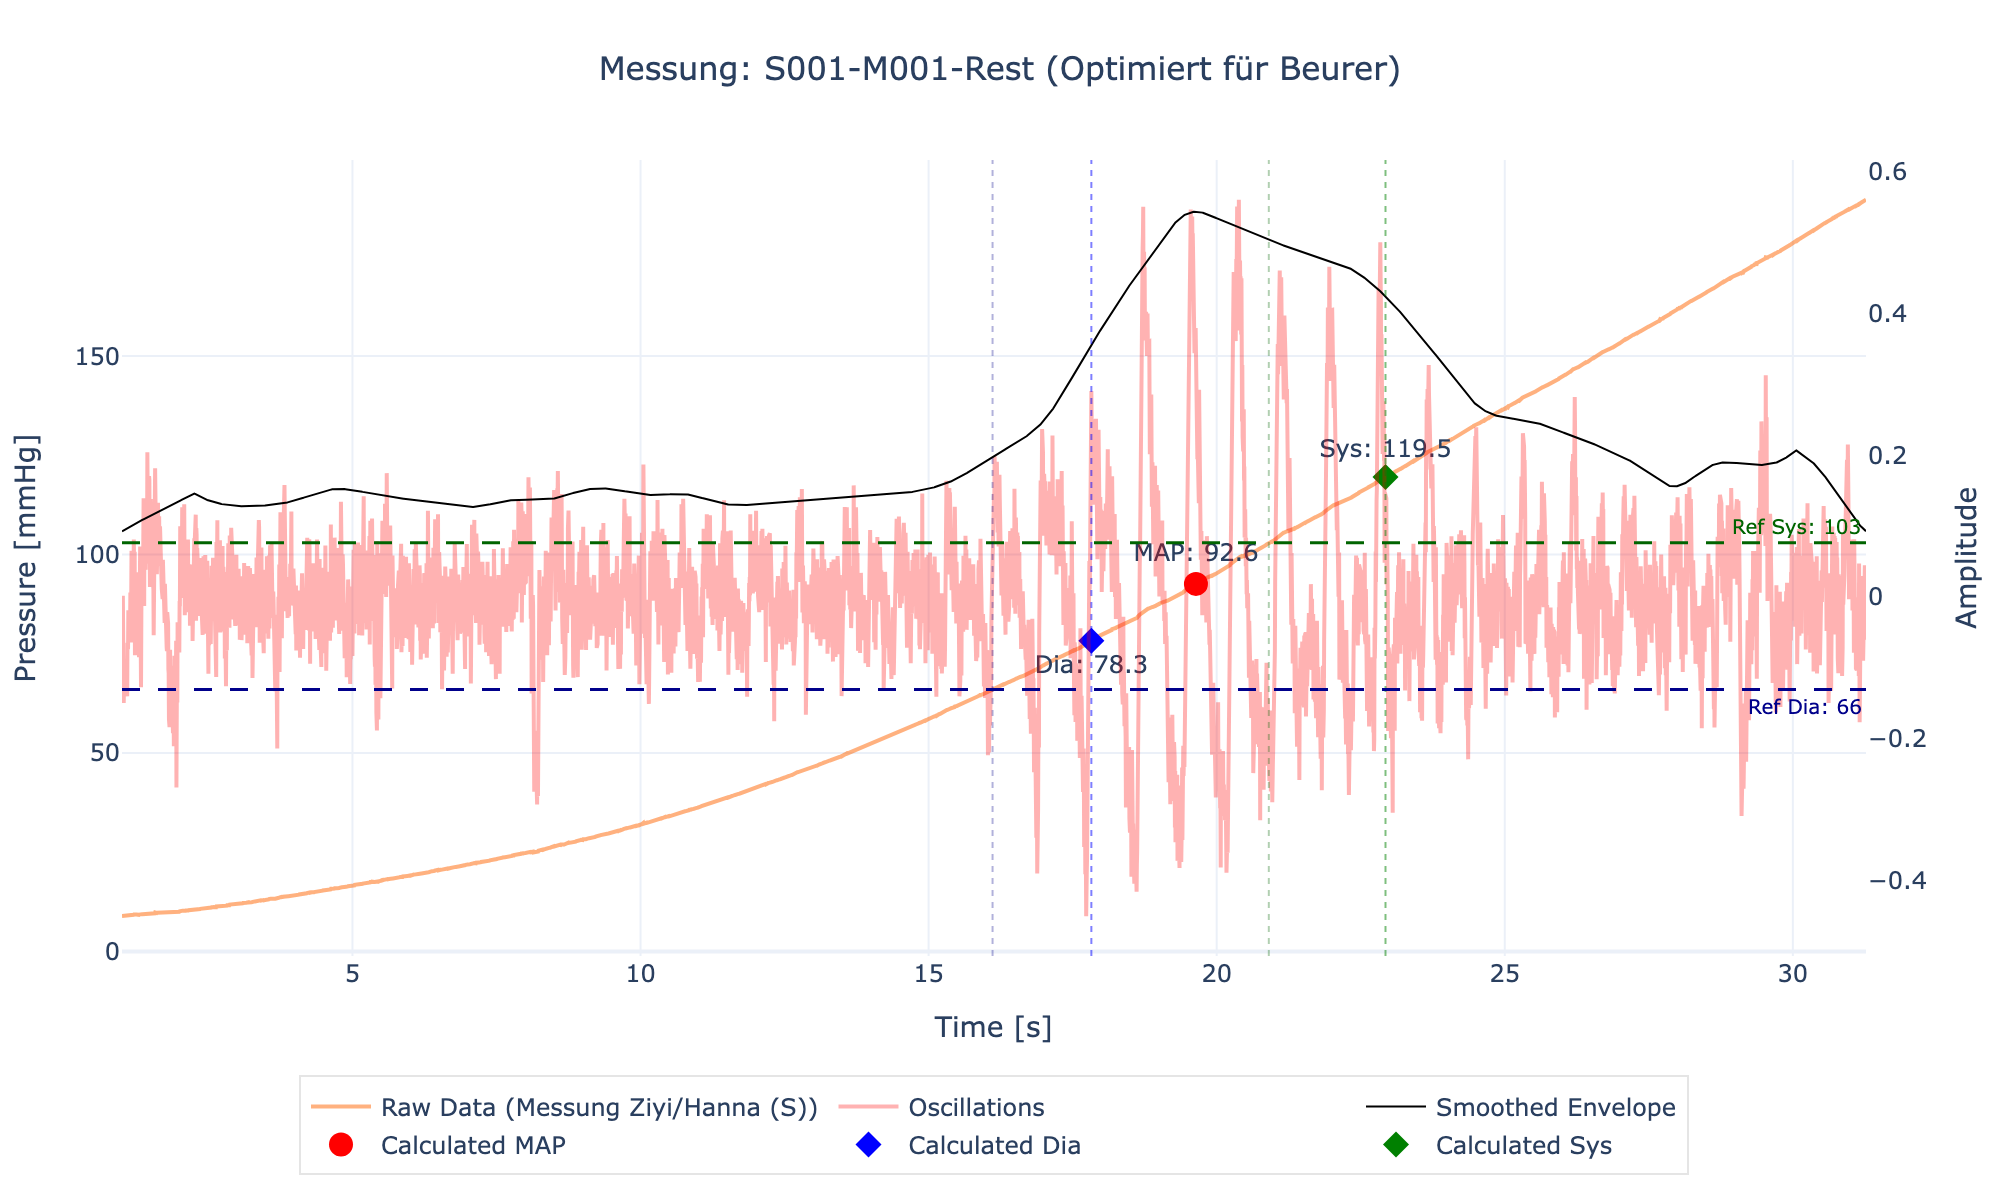
\includegraphics[width=\textwidth]{images/S001-M001-Rest_beurer.png}
        \caption{Optimiert für Beurer}
    \end{subfigure}
    \hfill
    \begin{subfigure}[b]{0.48\textwidth}
        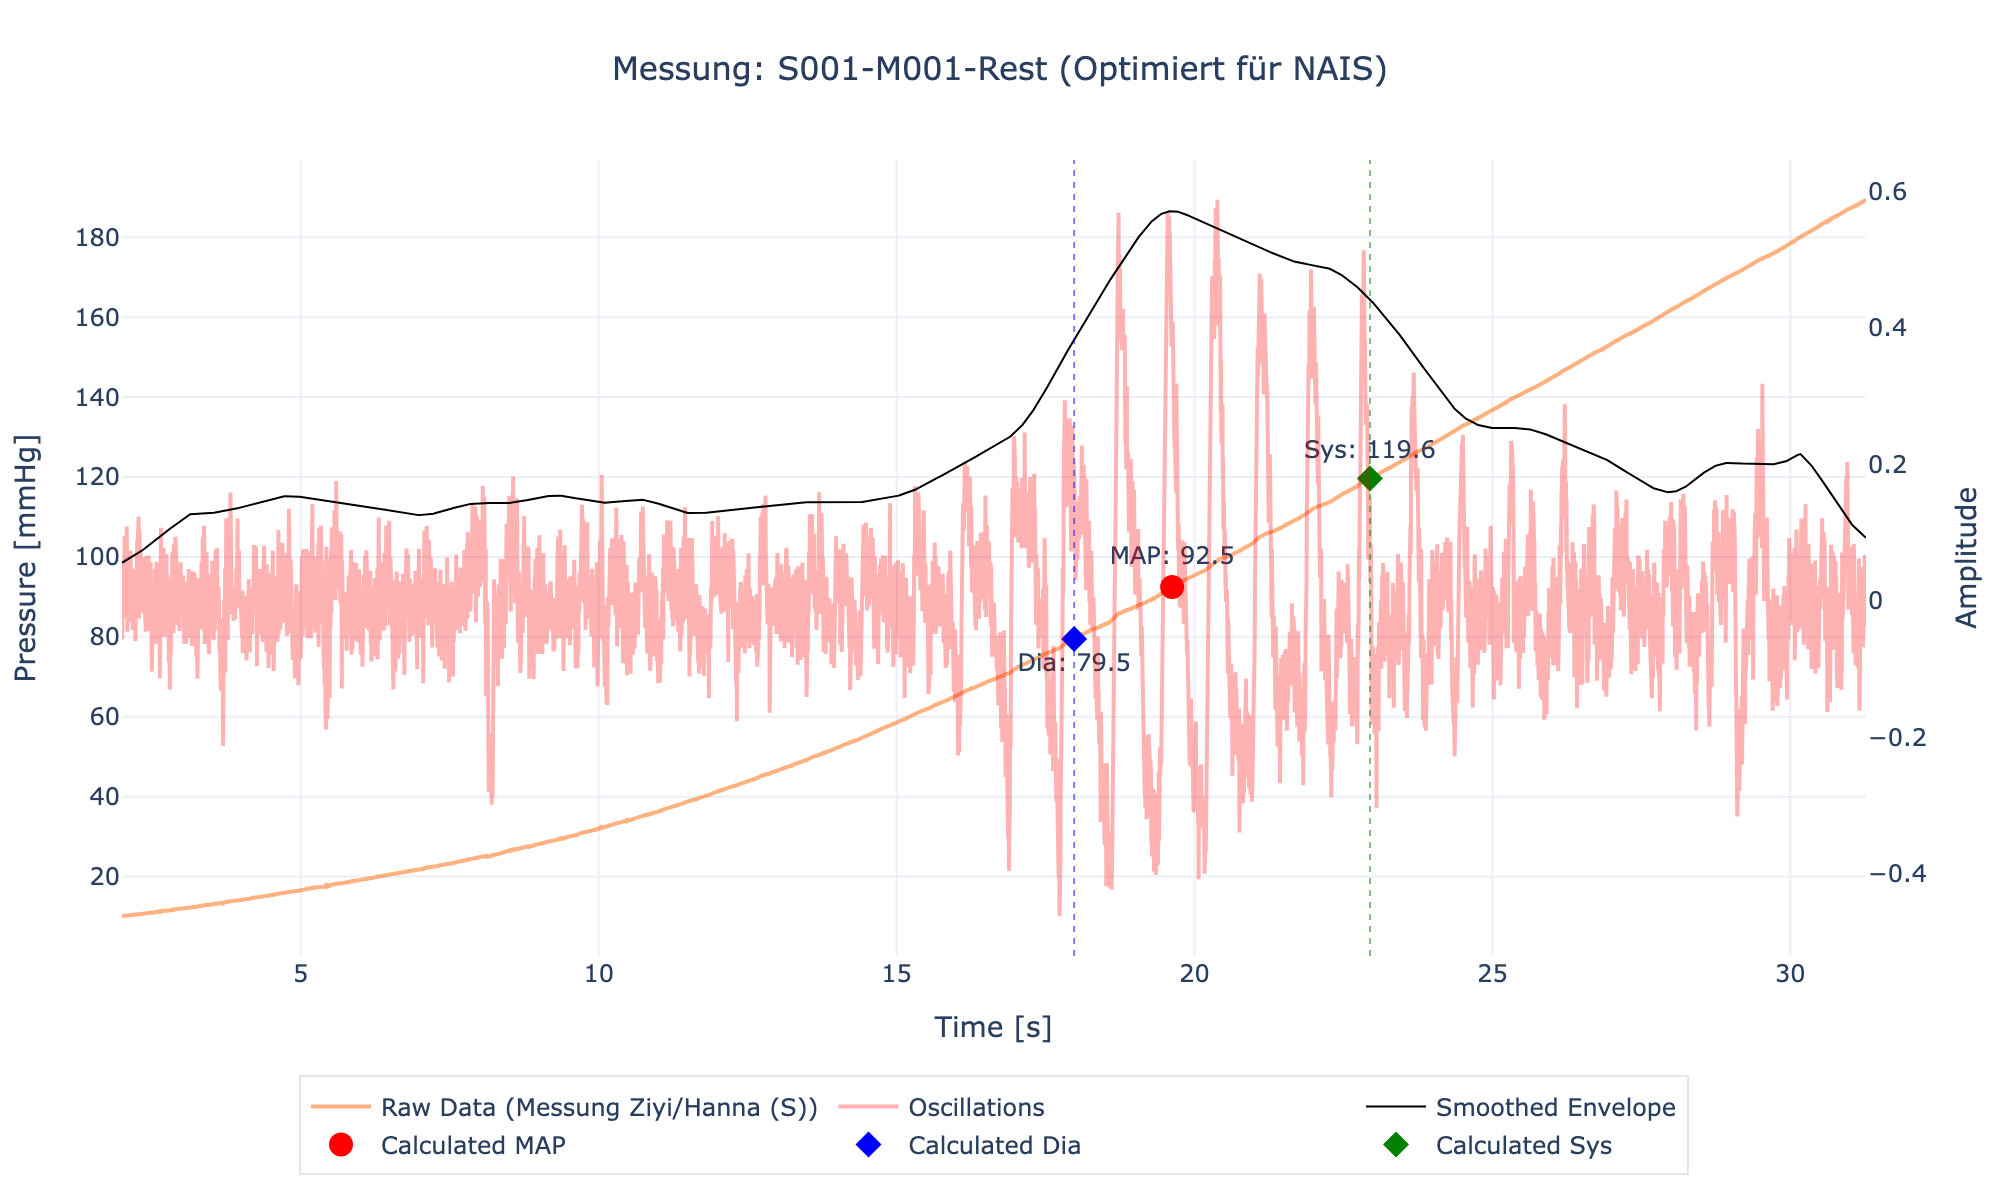
\includegraphics[width=\textwidth]{images/S001-M001-Rest_nais.png}
        \caption{Optimiert für NAIS}
    \end{subfigure}
    \caption{Einzelauswertung der Messung S001-M001-Rest mit verschiedenen Parametersätzen.}
\end{figure}
\newpage

\subsection*{Messung: S001-M002-Active}
\begin{figure}[H]
    \centering
    \begin{subfigure}[b]{0.8\textwidth}
        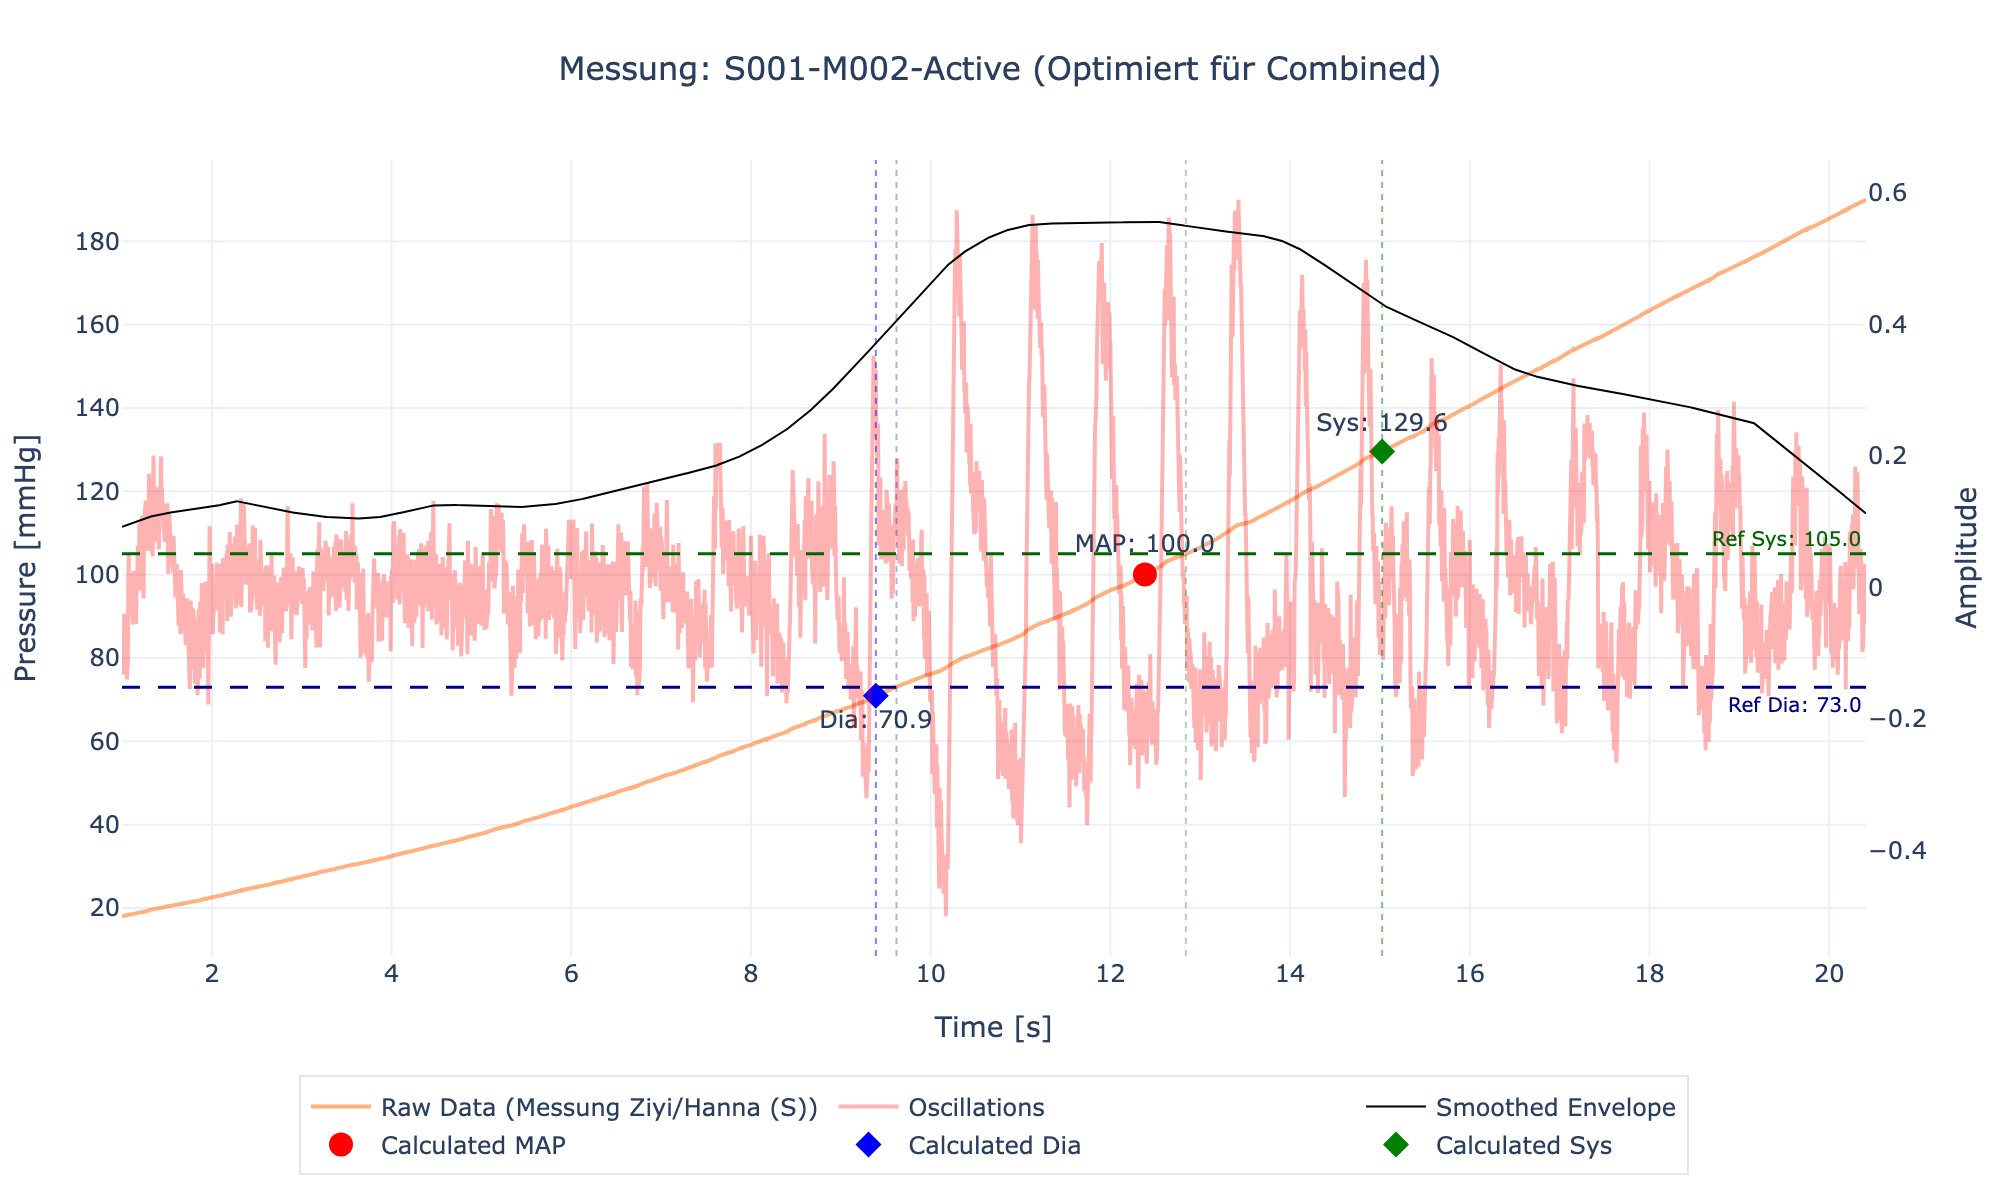
\includegraphics[width=\textwidth]{images/S001-M002-Active_combined.png}
        \caption{Optimiert für Beurer und NAIS (Kombiniert)}
    \end{subfigure} \\
    \begin{subfigure}[b]{0.48\textwidth}
        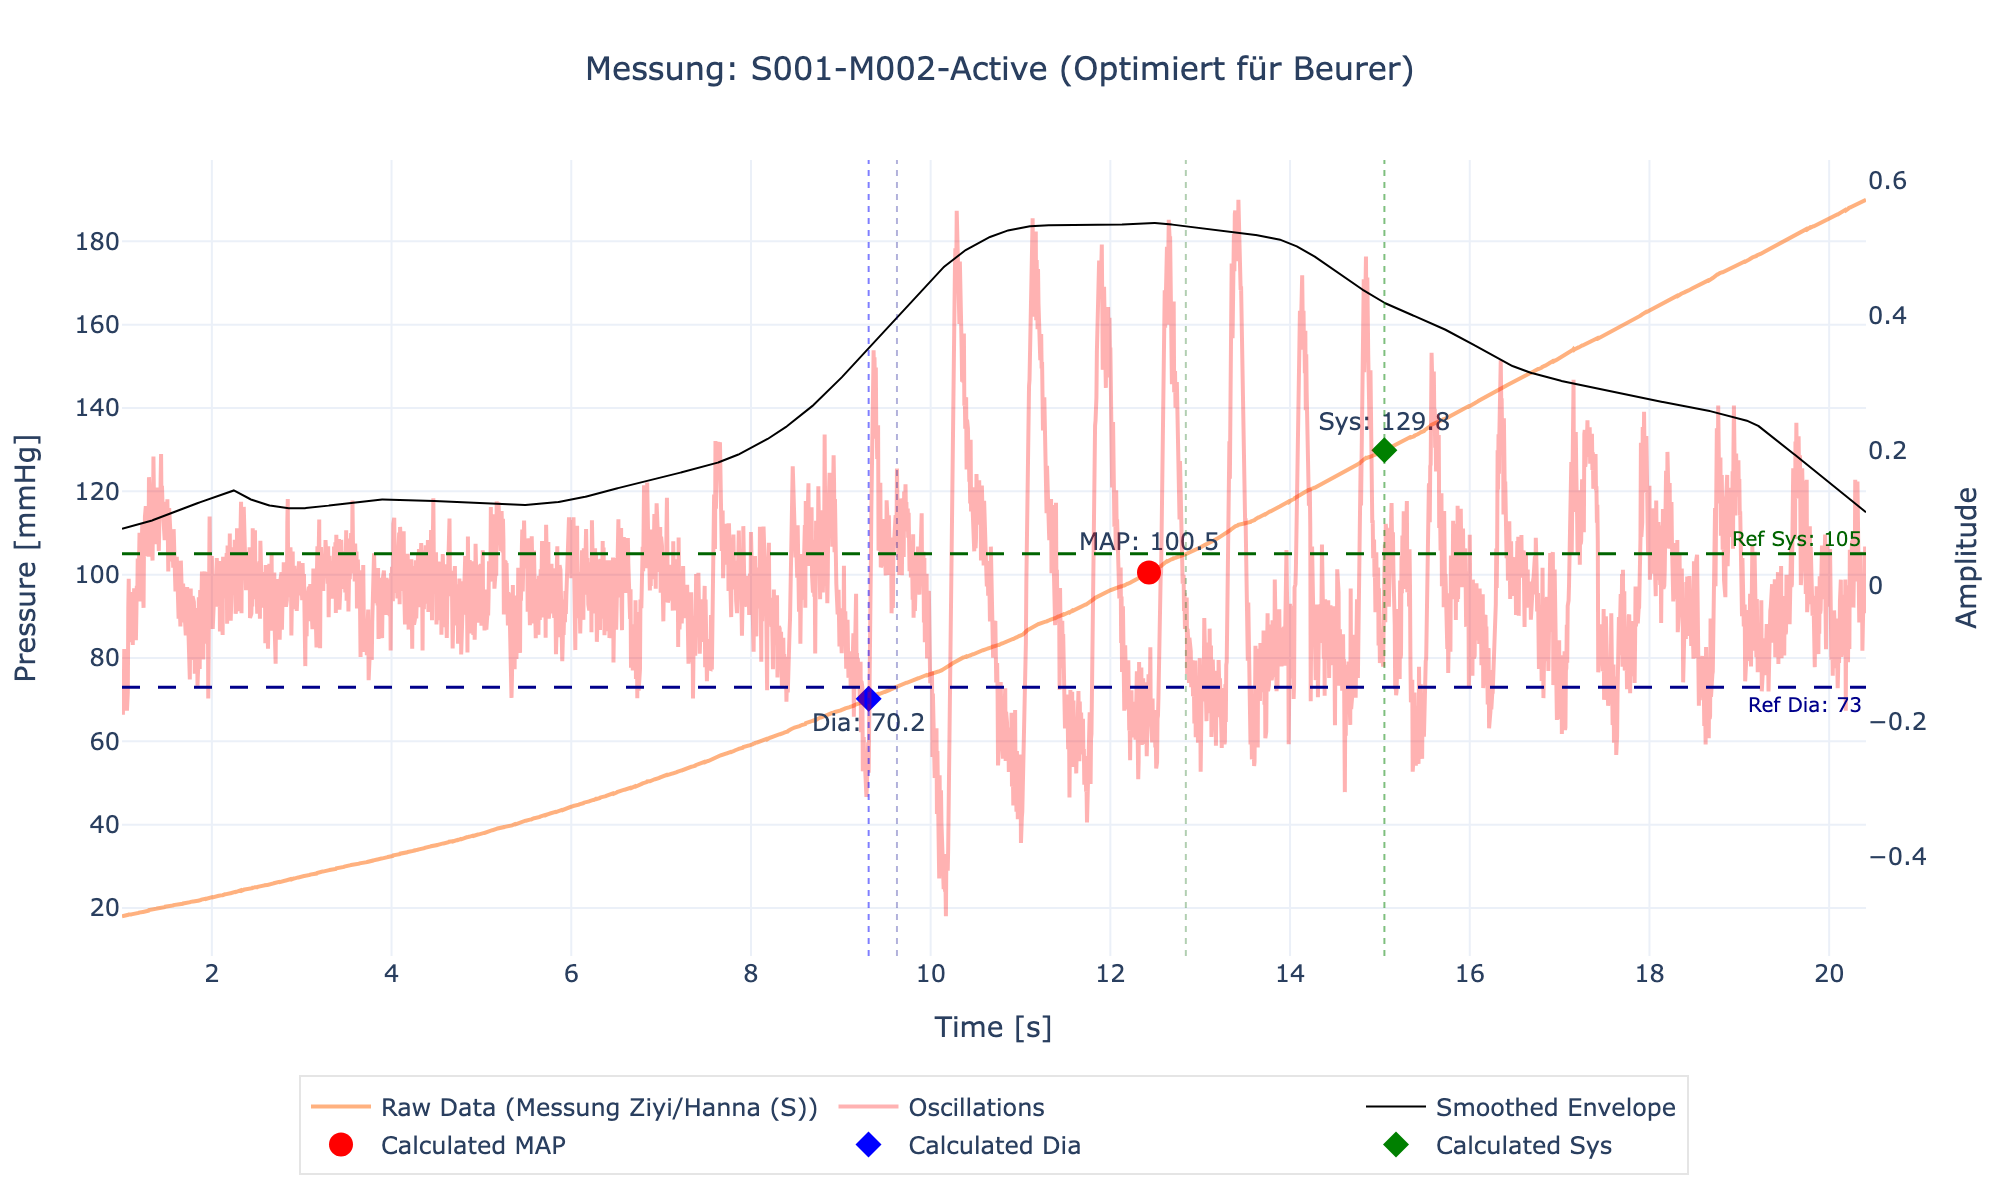
\includegraphics[width=\textwidth]{images/S001-M002-Active_beurer.png}
        \caption{Optimiert für Beurer}
    \end{subfigure}
    \hfill
    \begin{subfigure}[b]{0.48\textwidth}
        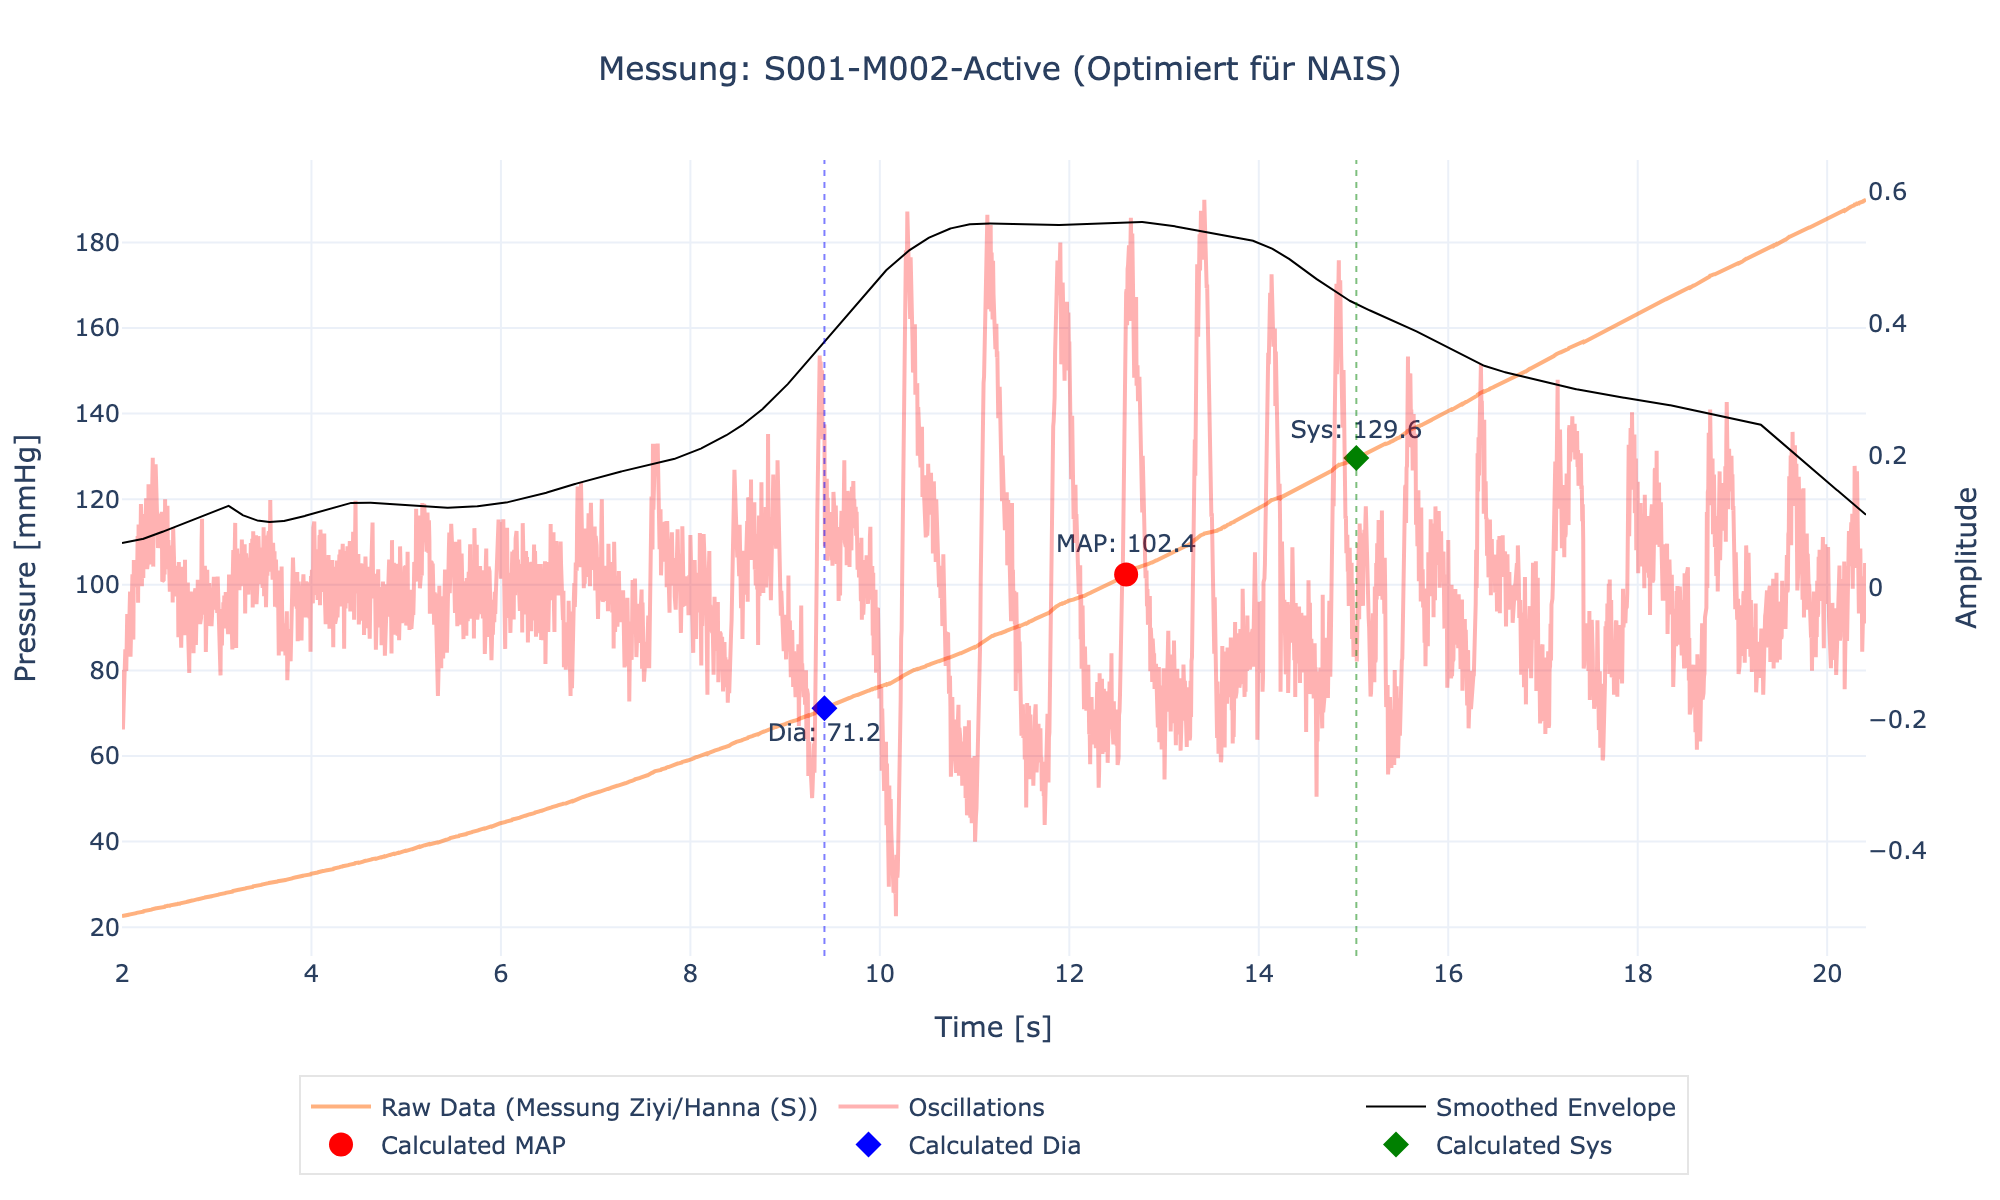
\includegraphics[width=\textwidth]{images/S001-M002-Active_nais.png}
        \caption{Optimiert für NAIS}
    \end{subfigure}
    \caption{Einzelauswertung der Messung S001-M002-Active mit verschiedenen Parametersätzen.}
\end{figure}
\newpage

\subsection*{Messung: S002-M001-Rest}
\begin{figure}[H]
    \centering
    \begin{subfigure}[b]{0.8\textwidth}
        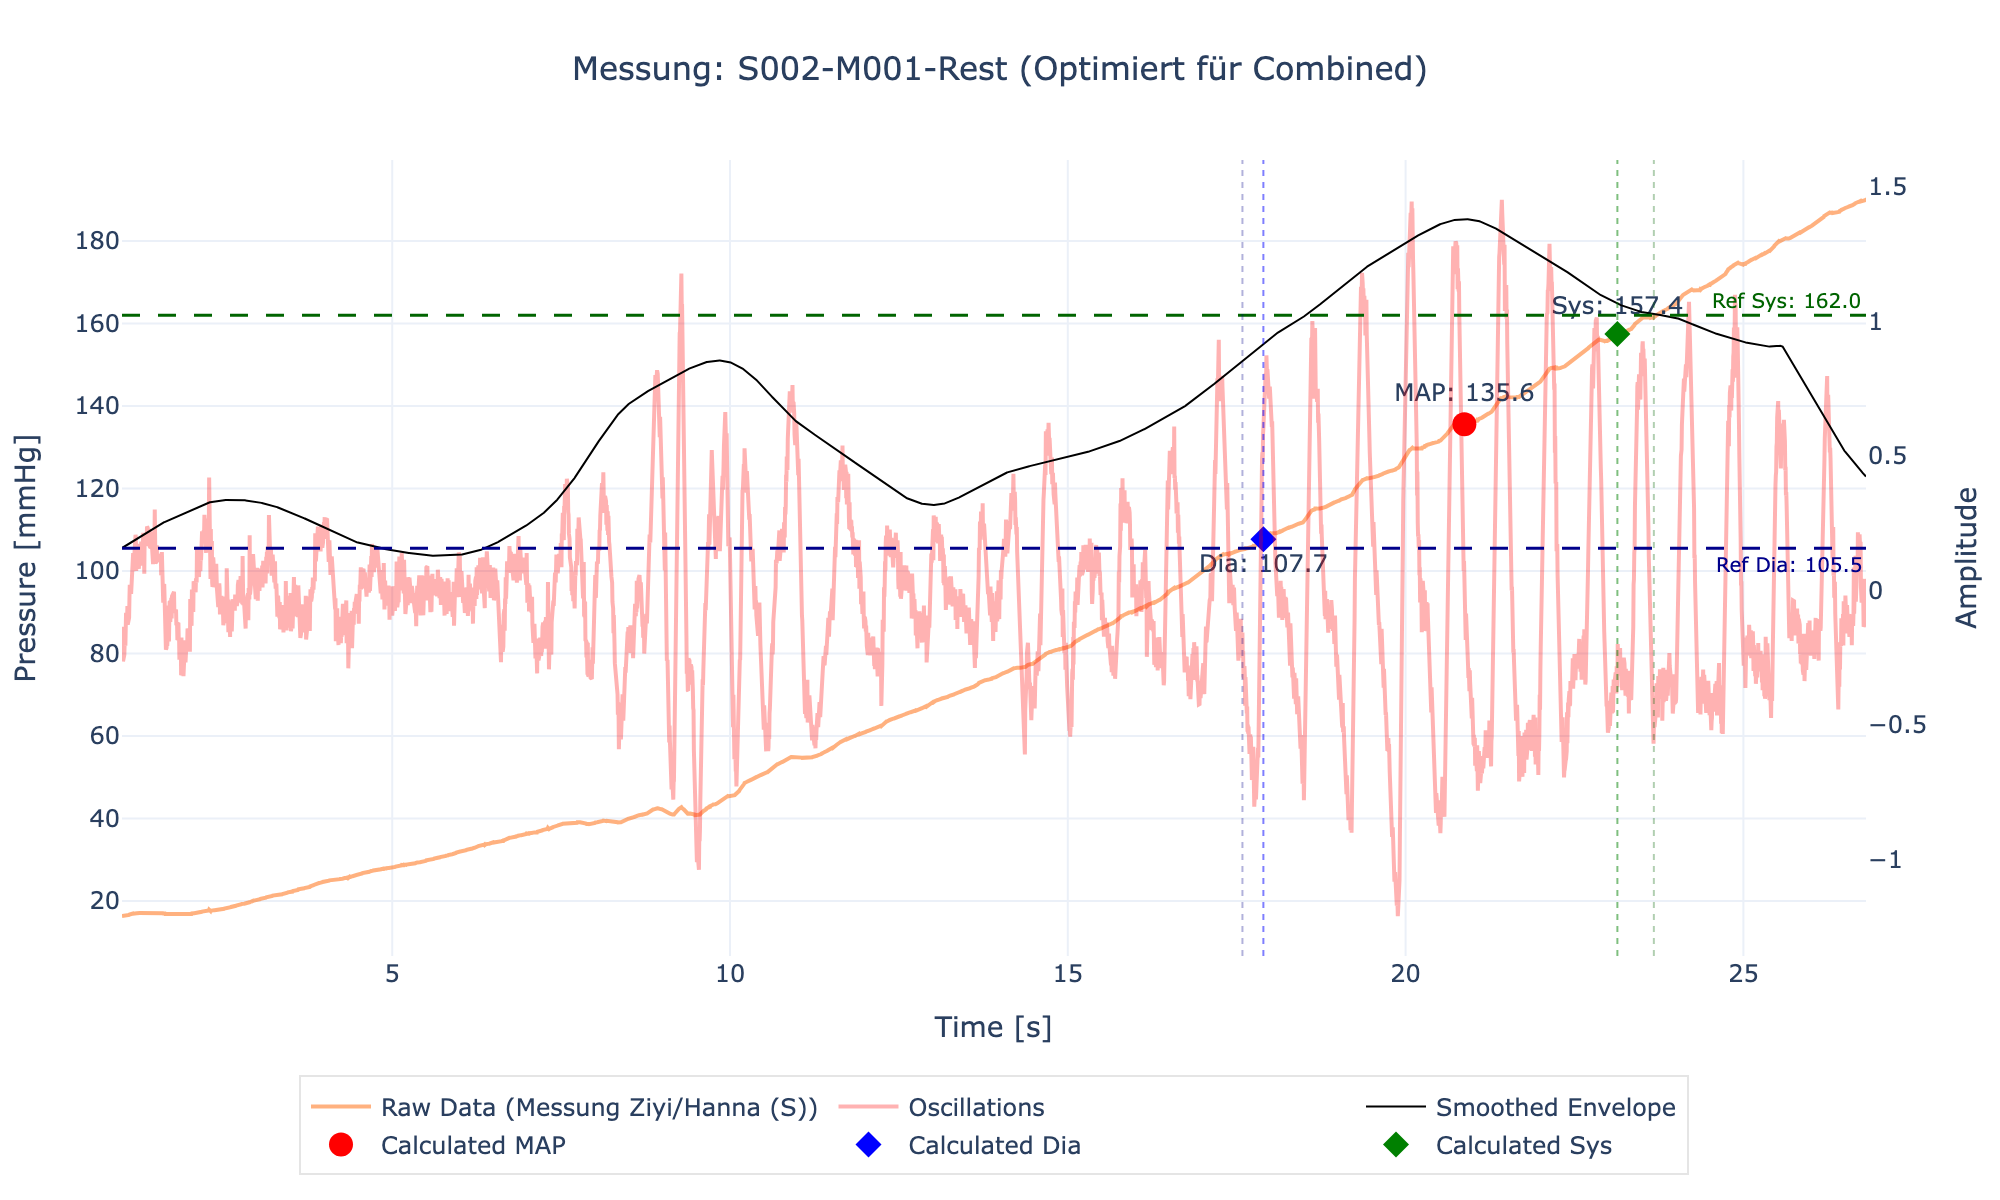
\includegraphics[width=\textwidth]{images/S002-M001-Rest_combined.png}
        \caption{Optimiert für Beurer und NAIS (Kombiniert)}
    \end{subfigure} \\
    \begin{subfigure}[b]{0.48\textwidth}
        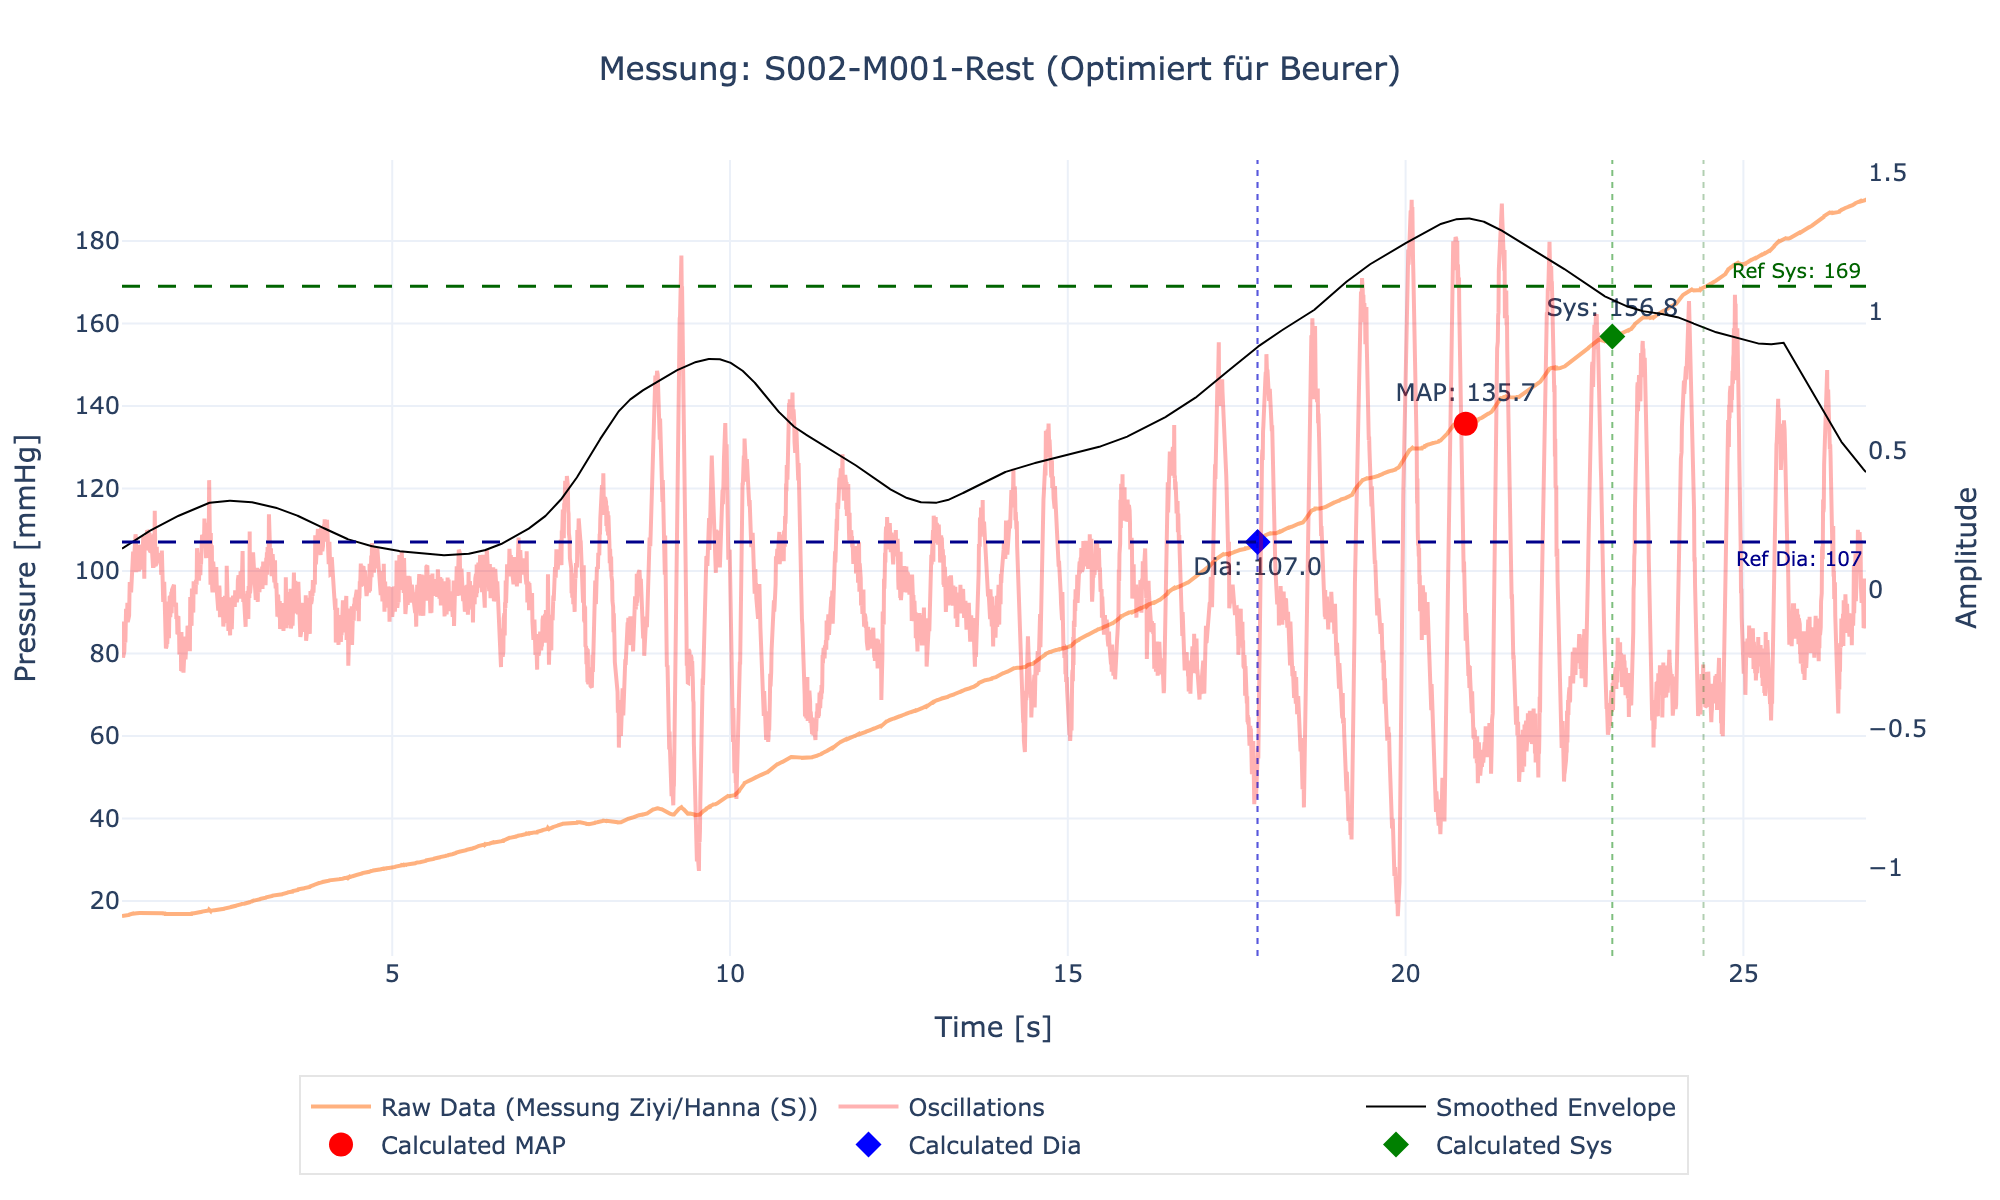
\includegraphics[width=\textwidth]{images/S002-M001-Rest_beurer.png}
        \caption{Optimiert für Beurer}
    \end{subfigure}
    \hfill
    \begin{subfigure}[b]{0.48\textwidth}
        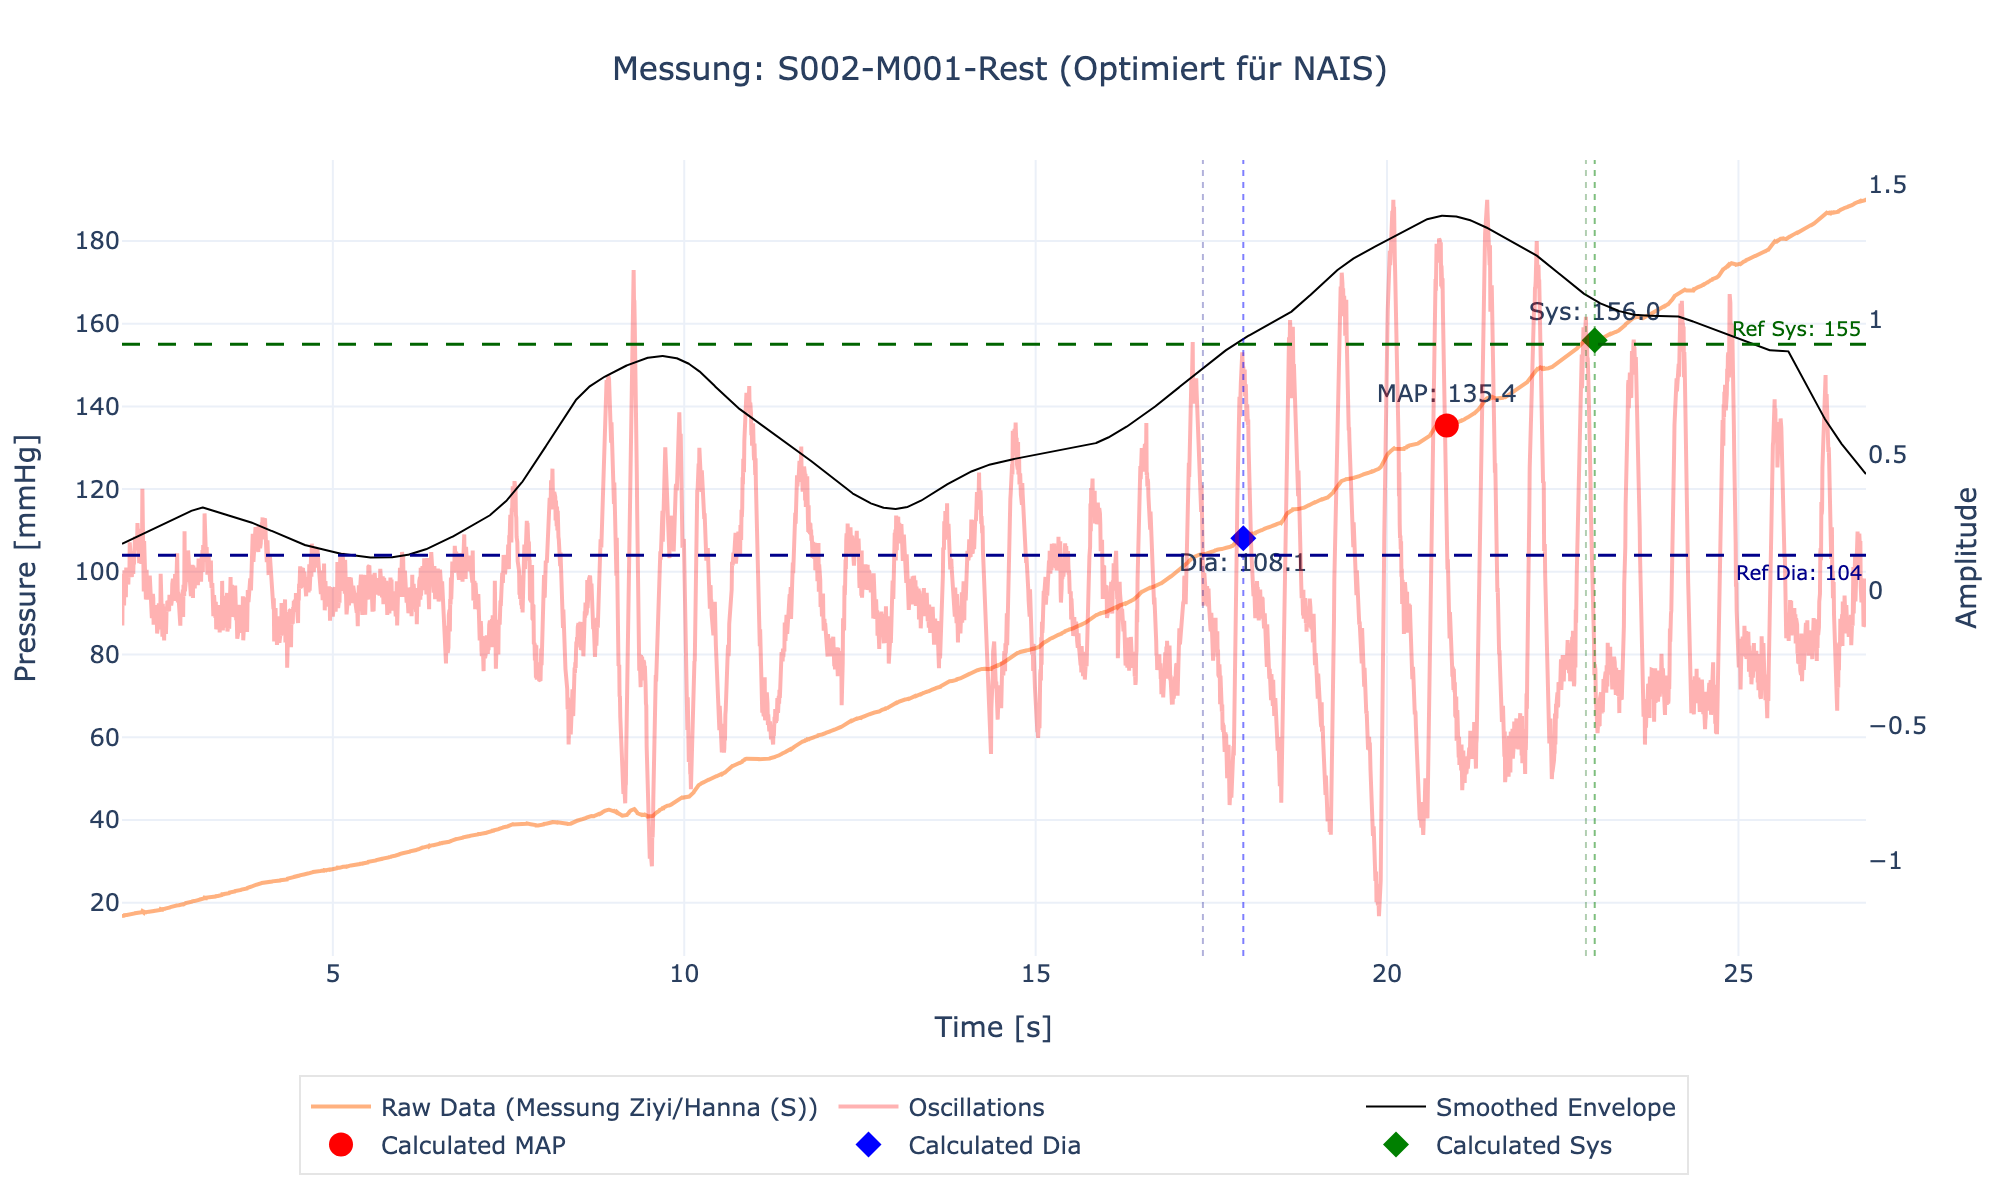
\includegraphics[width=\textwidth]{images/S002-M001-Rest_nais.png}
        \caption{Optimiert für NAIS}
    \end{subfigure}
    \caption{Einzelauswertung der Messung S002-M001-Rest mit verschiedenen Parametersätzen.}
\end{figure}
\newpage

\subsection*{Messung: S002-M002-Active}
\begin{figure}[H]
    \centering
    \begin{subfigure}[b]{0.8\textwidth}
        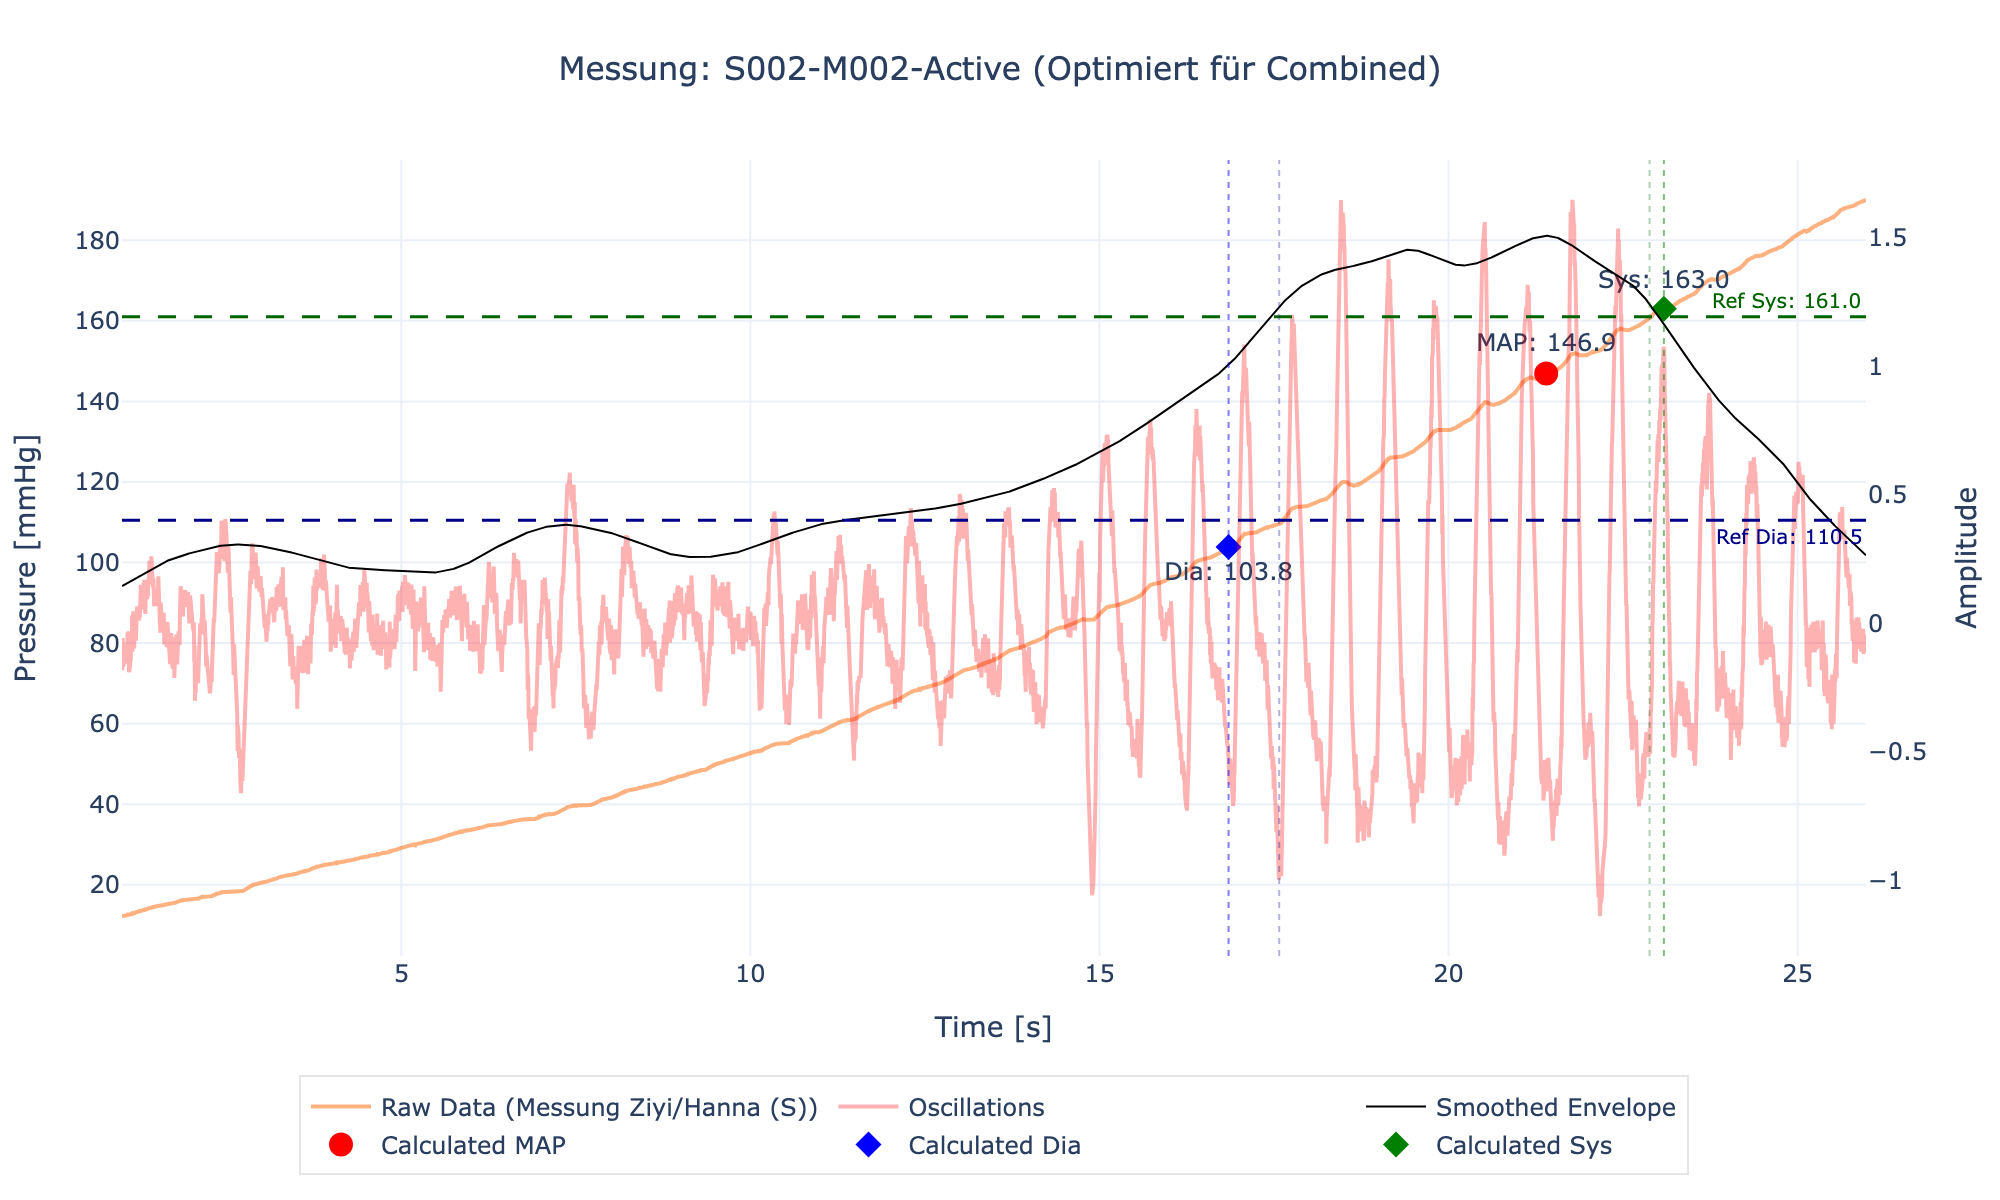
\includegraphics[width=\textwidth]{images/S002-M002-Active_combined.png}
        \caption{Optimiert für Beurer und NAIS (Kombiniert)}
    \end{subfigure} \\
    \begin{subfigure}[b]{0.48\textwidth}
        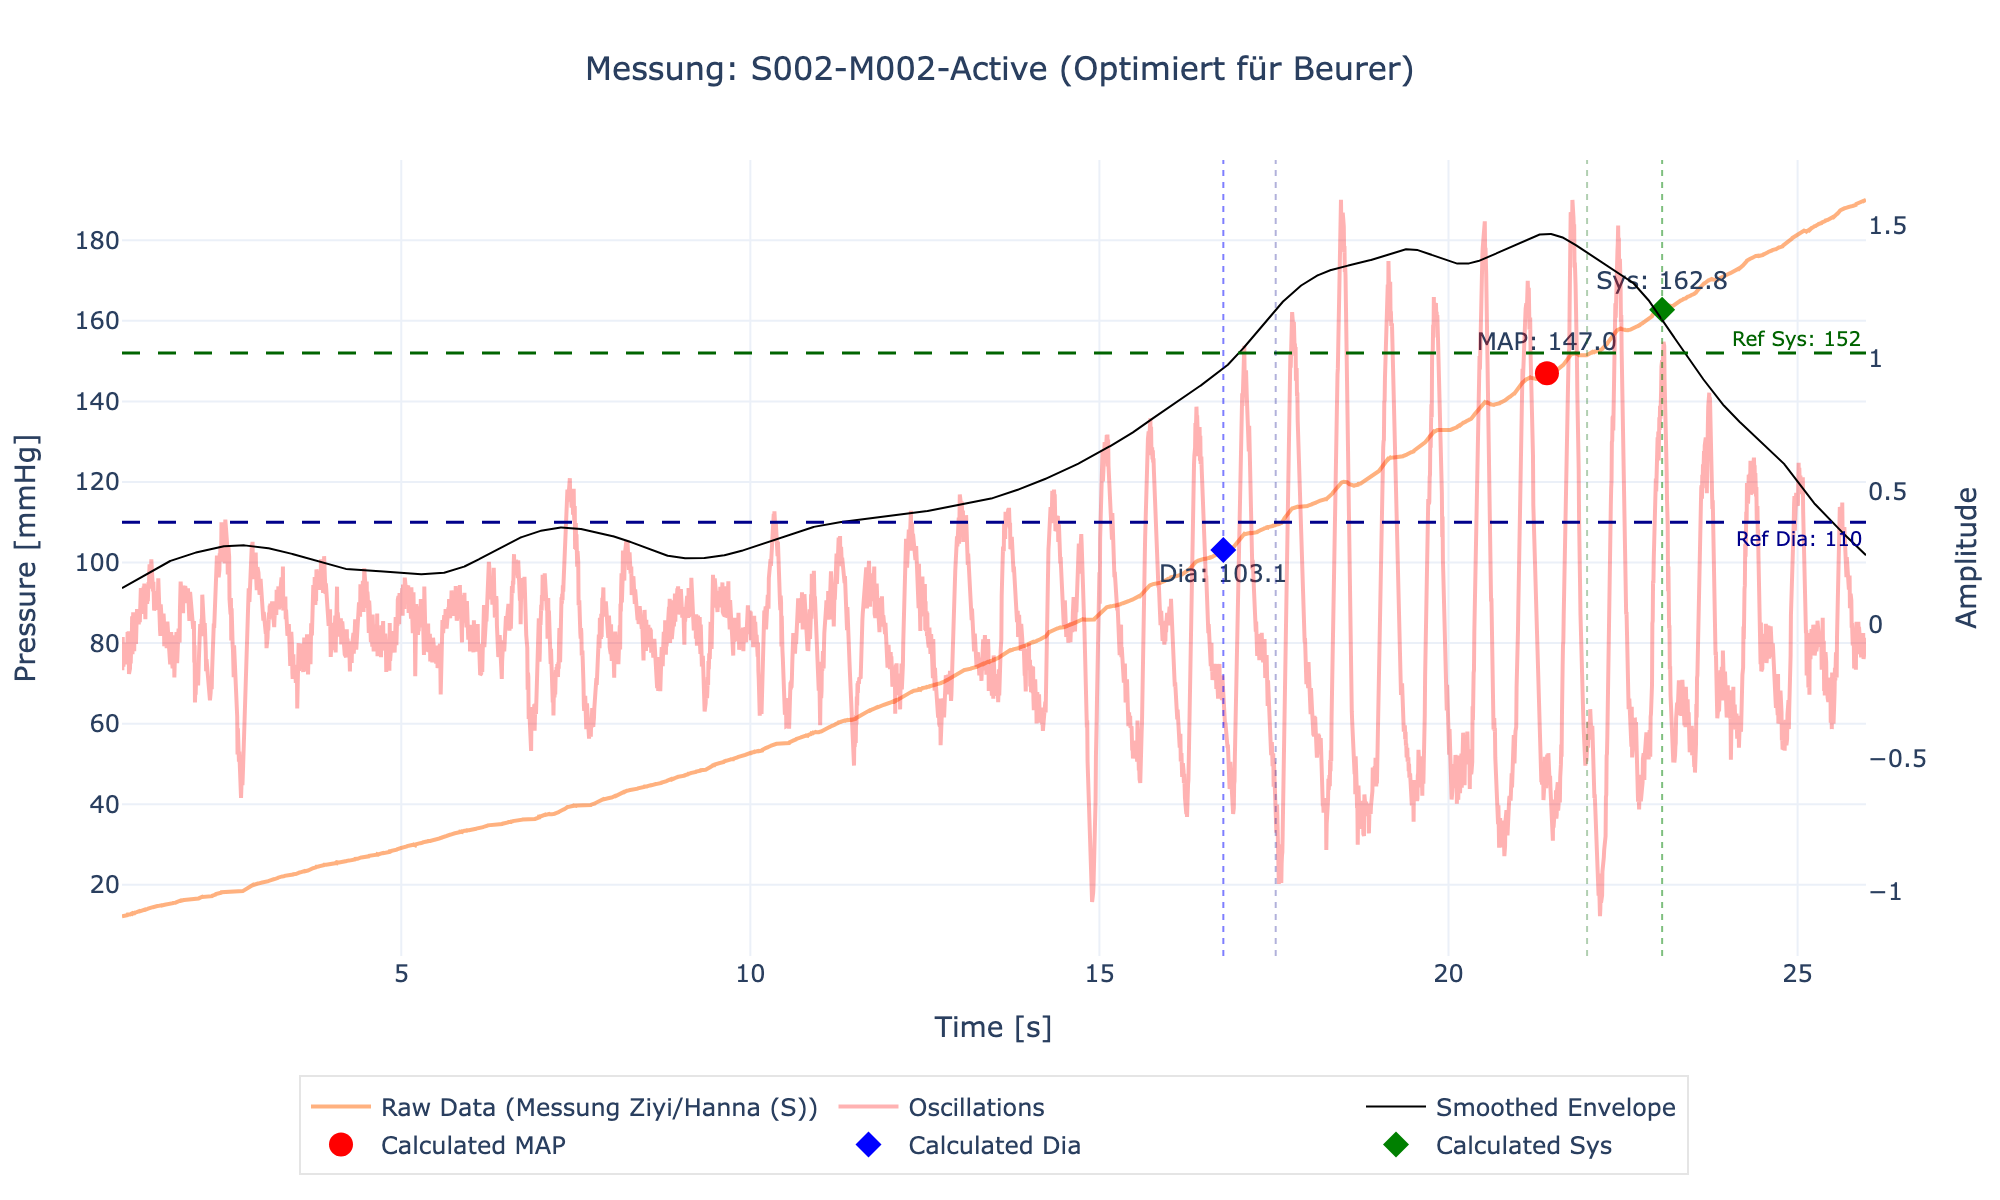
\includegraphics[width=\textwidth]{images/S002-M002-Active_beurer.png}
        \caption{Optimiert für Beurer}
    \end{subfigure}
    \hfill
    \begin{subfigure}[b]{0.48\textwidth}
        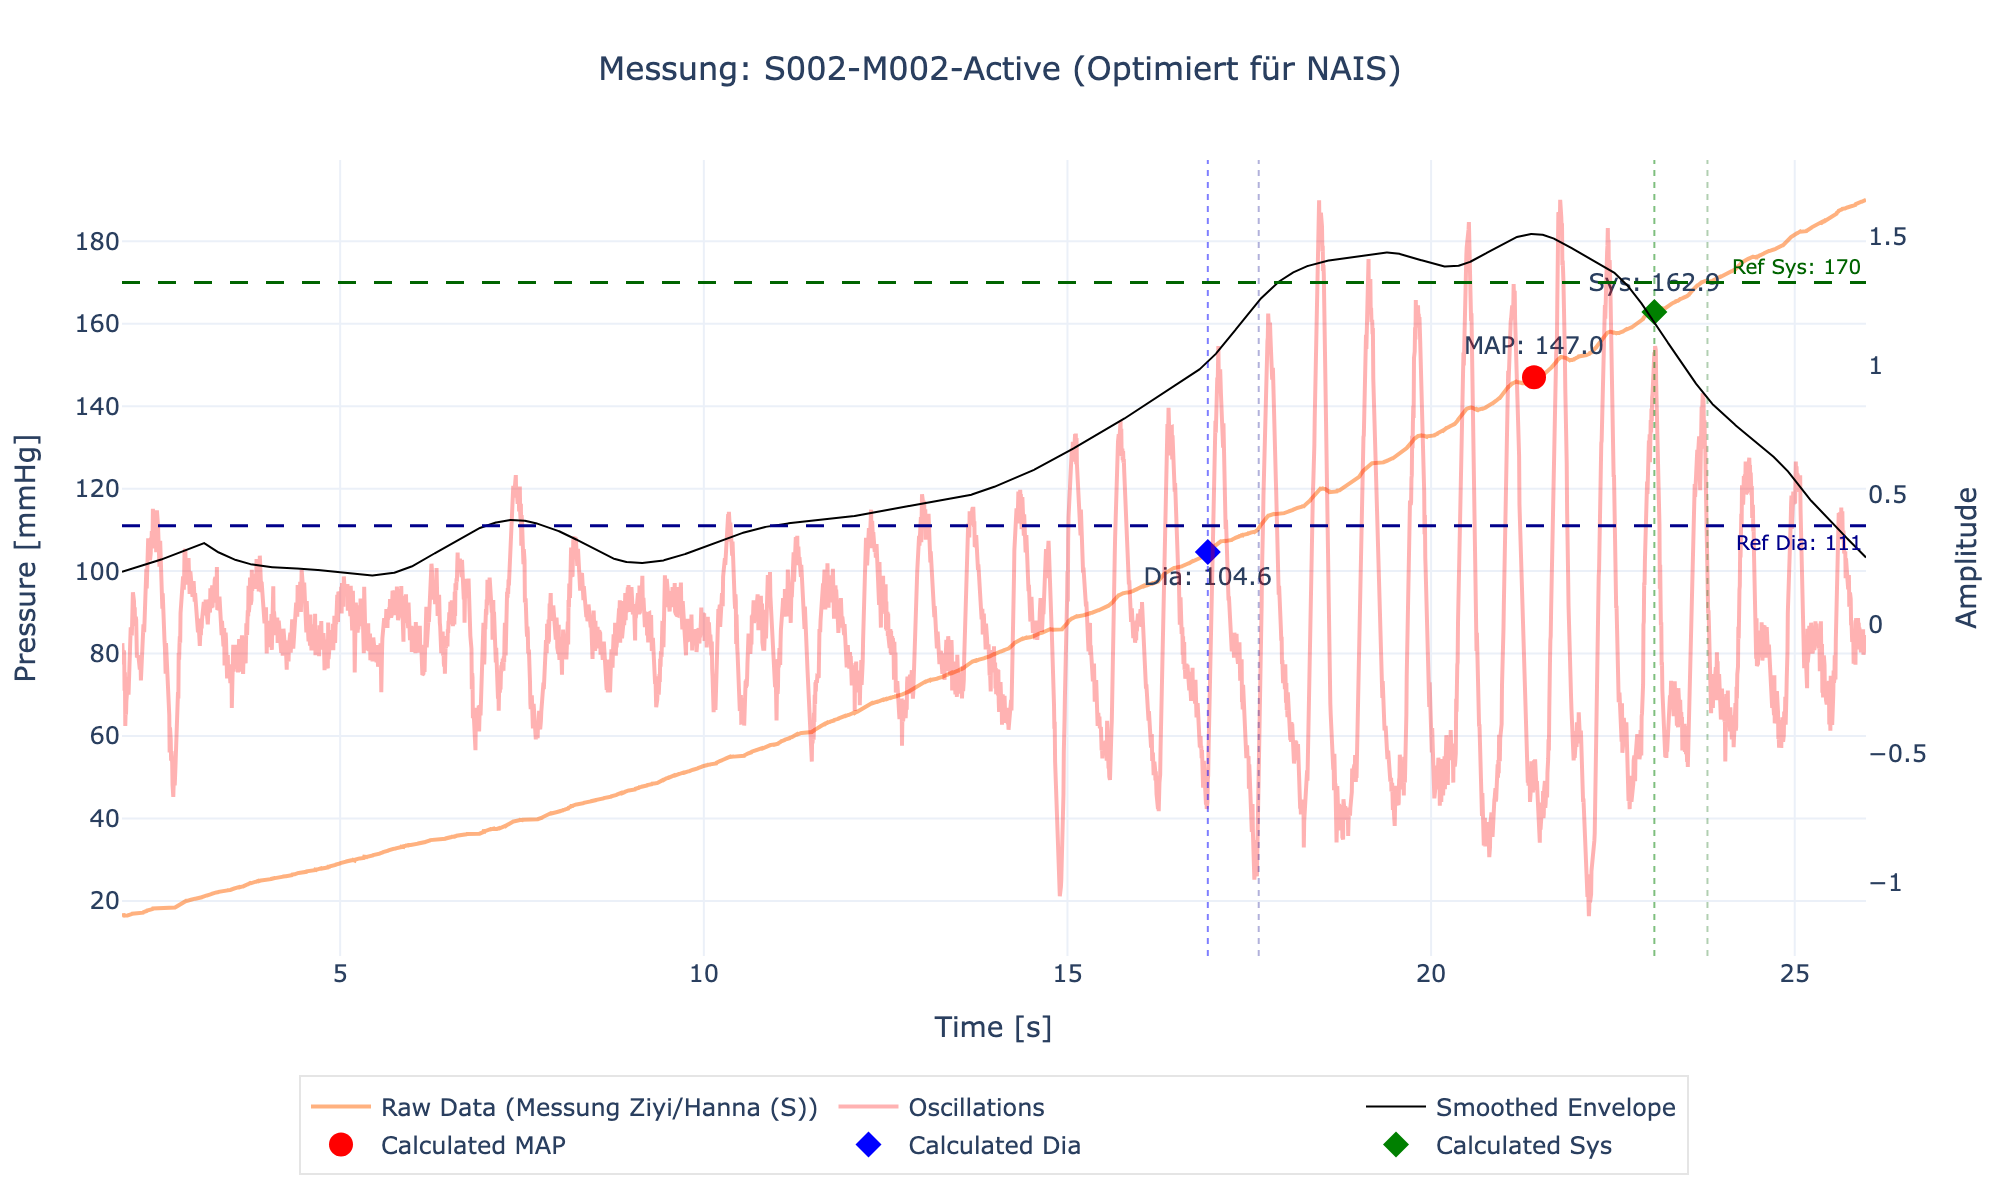
\includegraphics[width=\textwidth]{images/S002-M002-Active_nais.png}
        \caption{Optimiert für NAIS}
    \end{subfigure}
    \caption{Einzelauswertung der Messung S002-M002-Active mit verschiedenen Parametersätzen.}
\end{figure}
\newpage

\subsection*{Messung: S003-M001-Rest}
\begin{figure}[H]
    \centering
    \begin{subfigure}[b]{0.8\textwidth}
        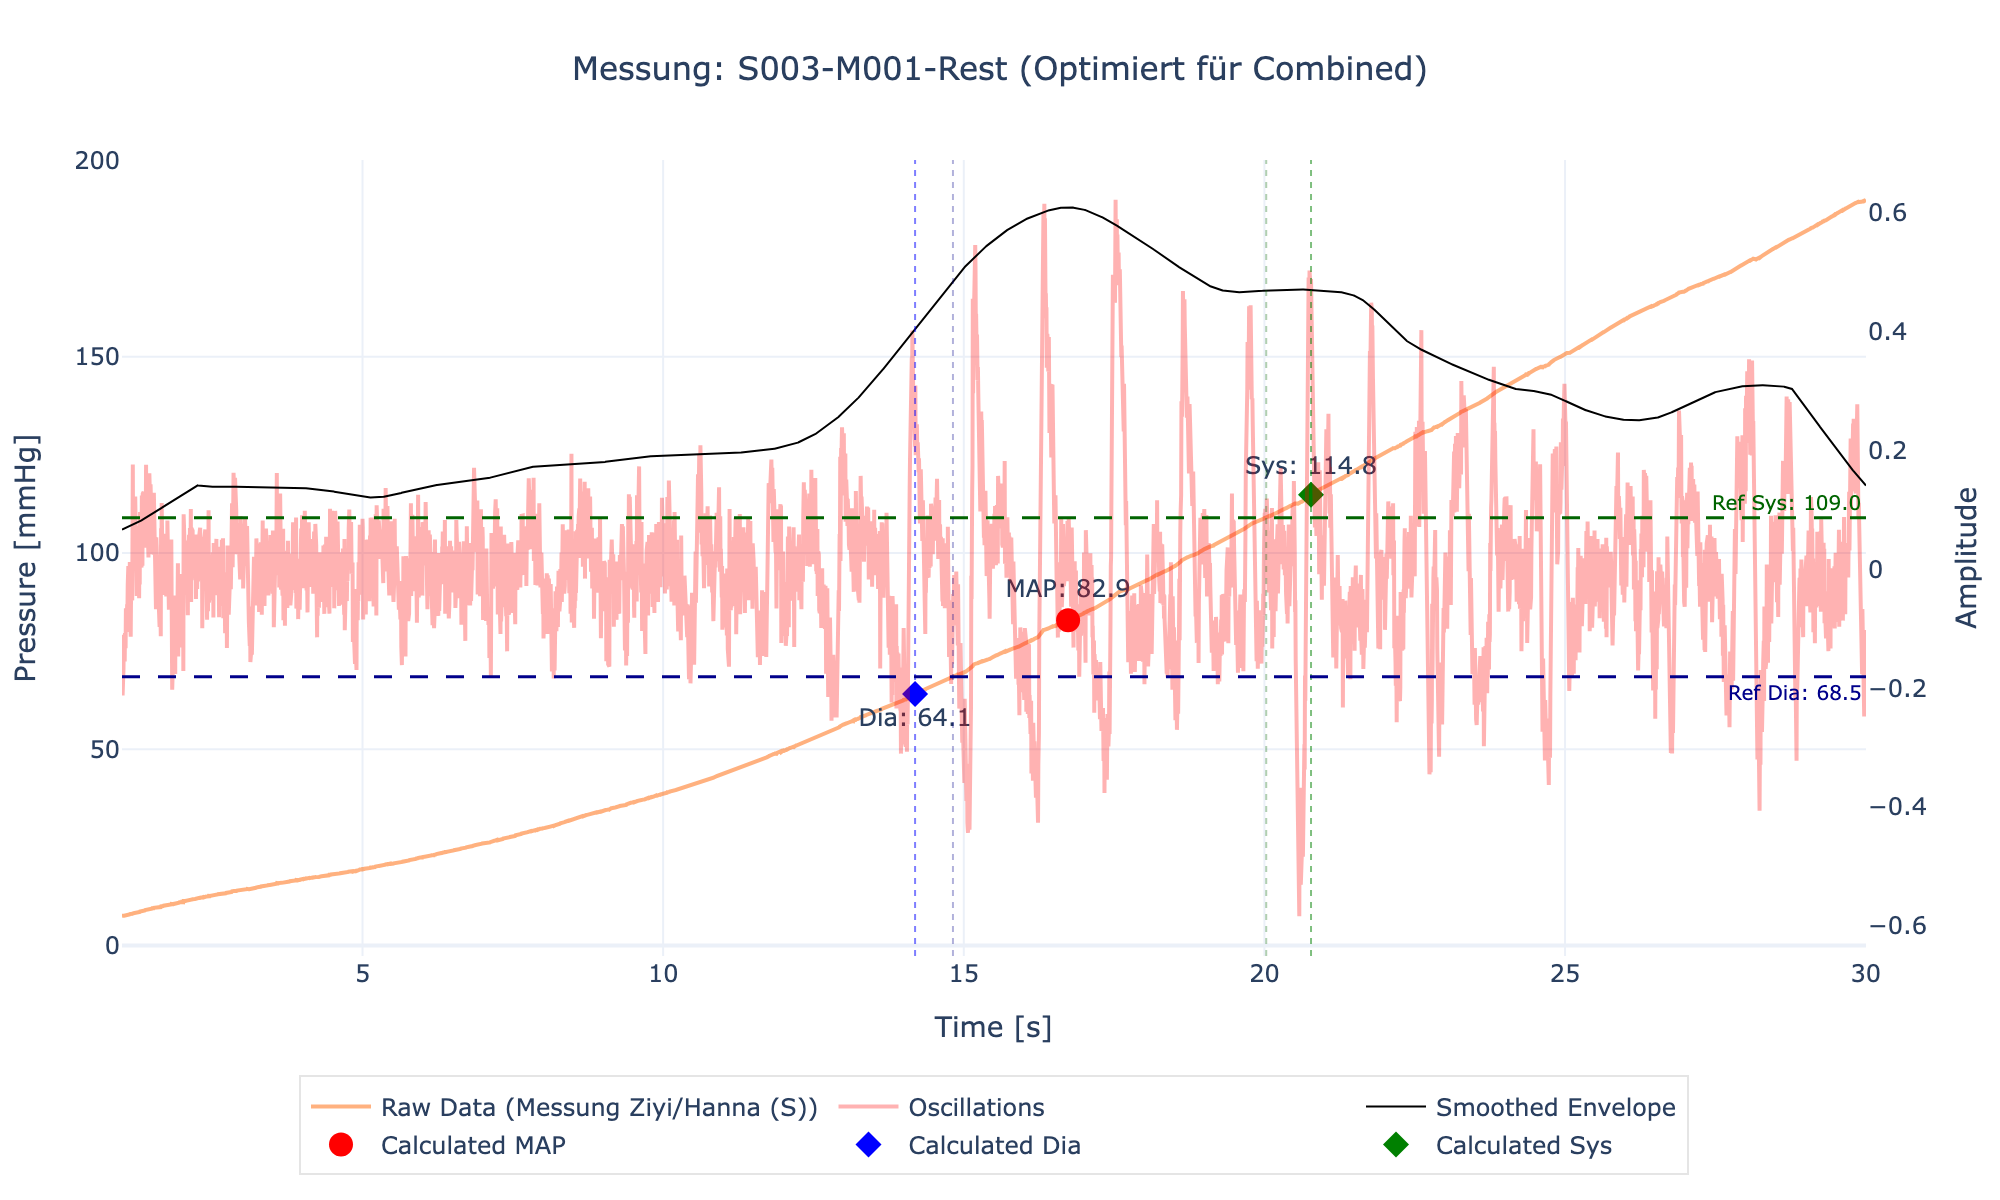
\includegraphics[width=\textwidth]{images/S003-M001-Rest_combined.png}
        \caption{Optimiert für Beurer und NAIS (Kombiniert)}
    \end{subfigure} \\
    \begin{subfigure}[b]{0.48\textwidth}
        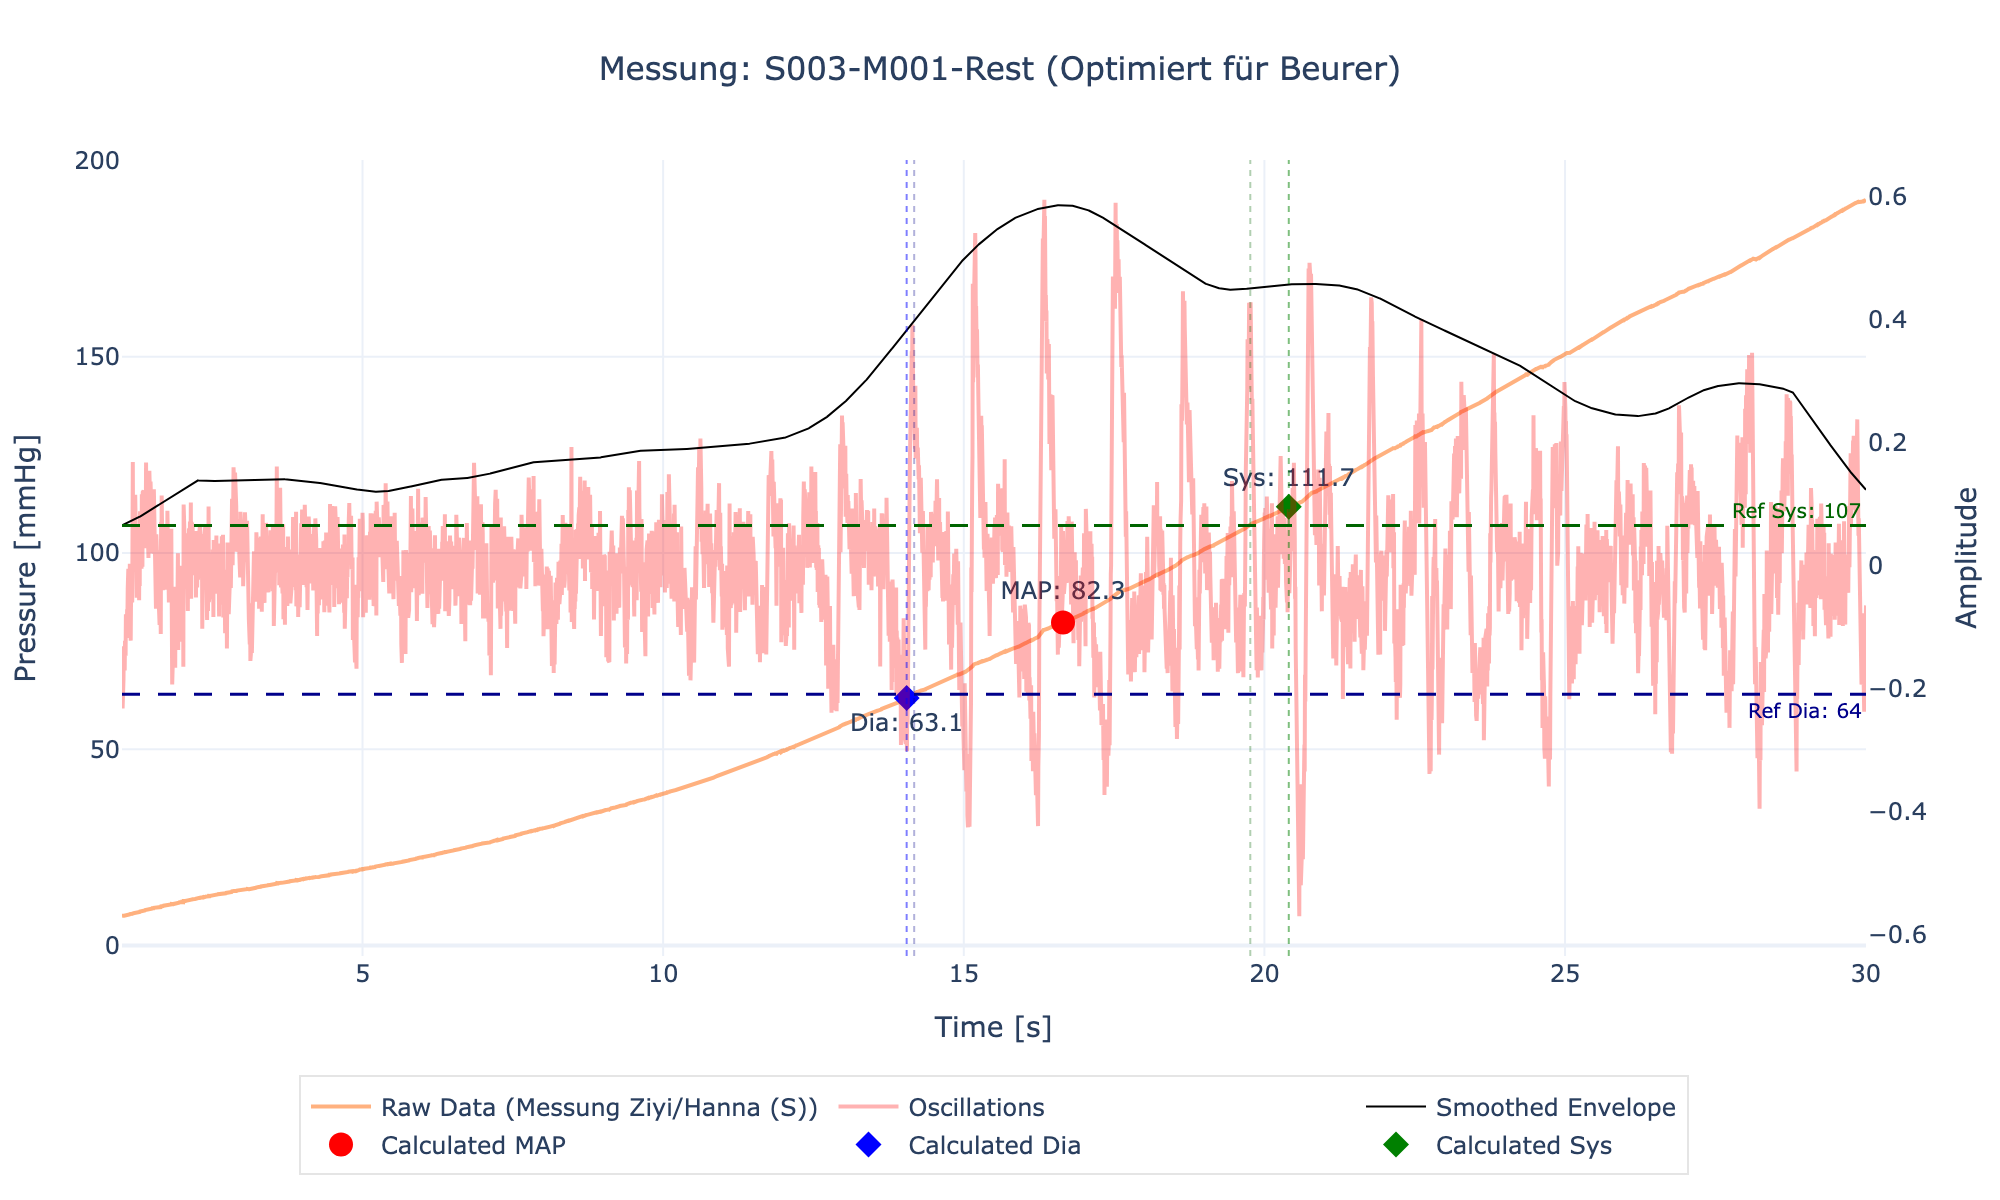
\includegraphics[width=\textwidth]{images/S003-M001-Rest_beurer.png}
        \caption{Optimiert für Beurer}
    \end{subfigure}
    \hfill
    \begin{subfigure}[b]{0.48\textwidth}
        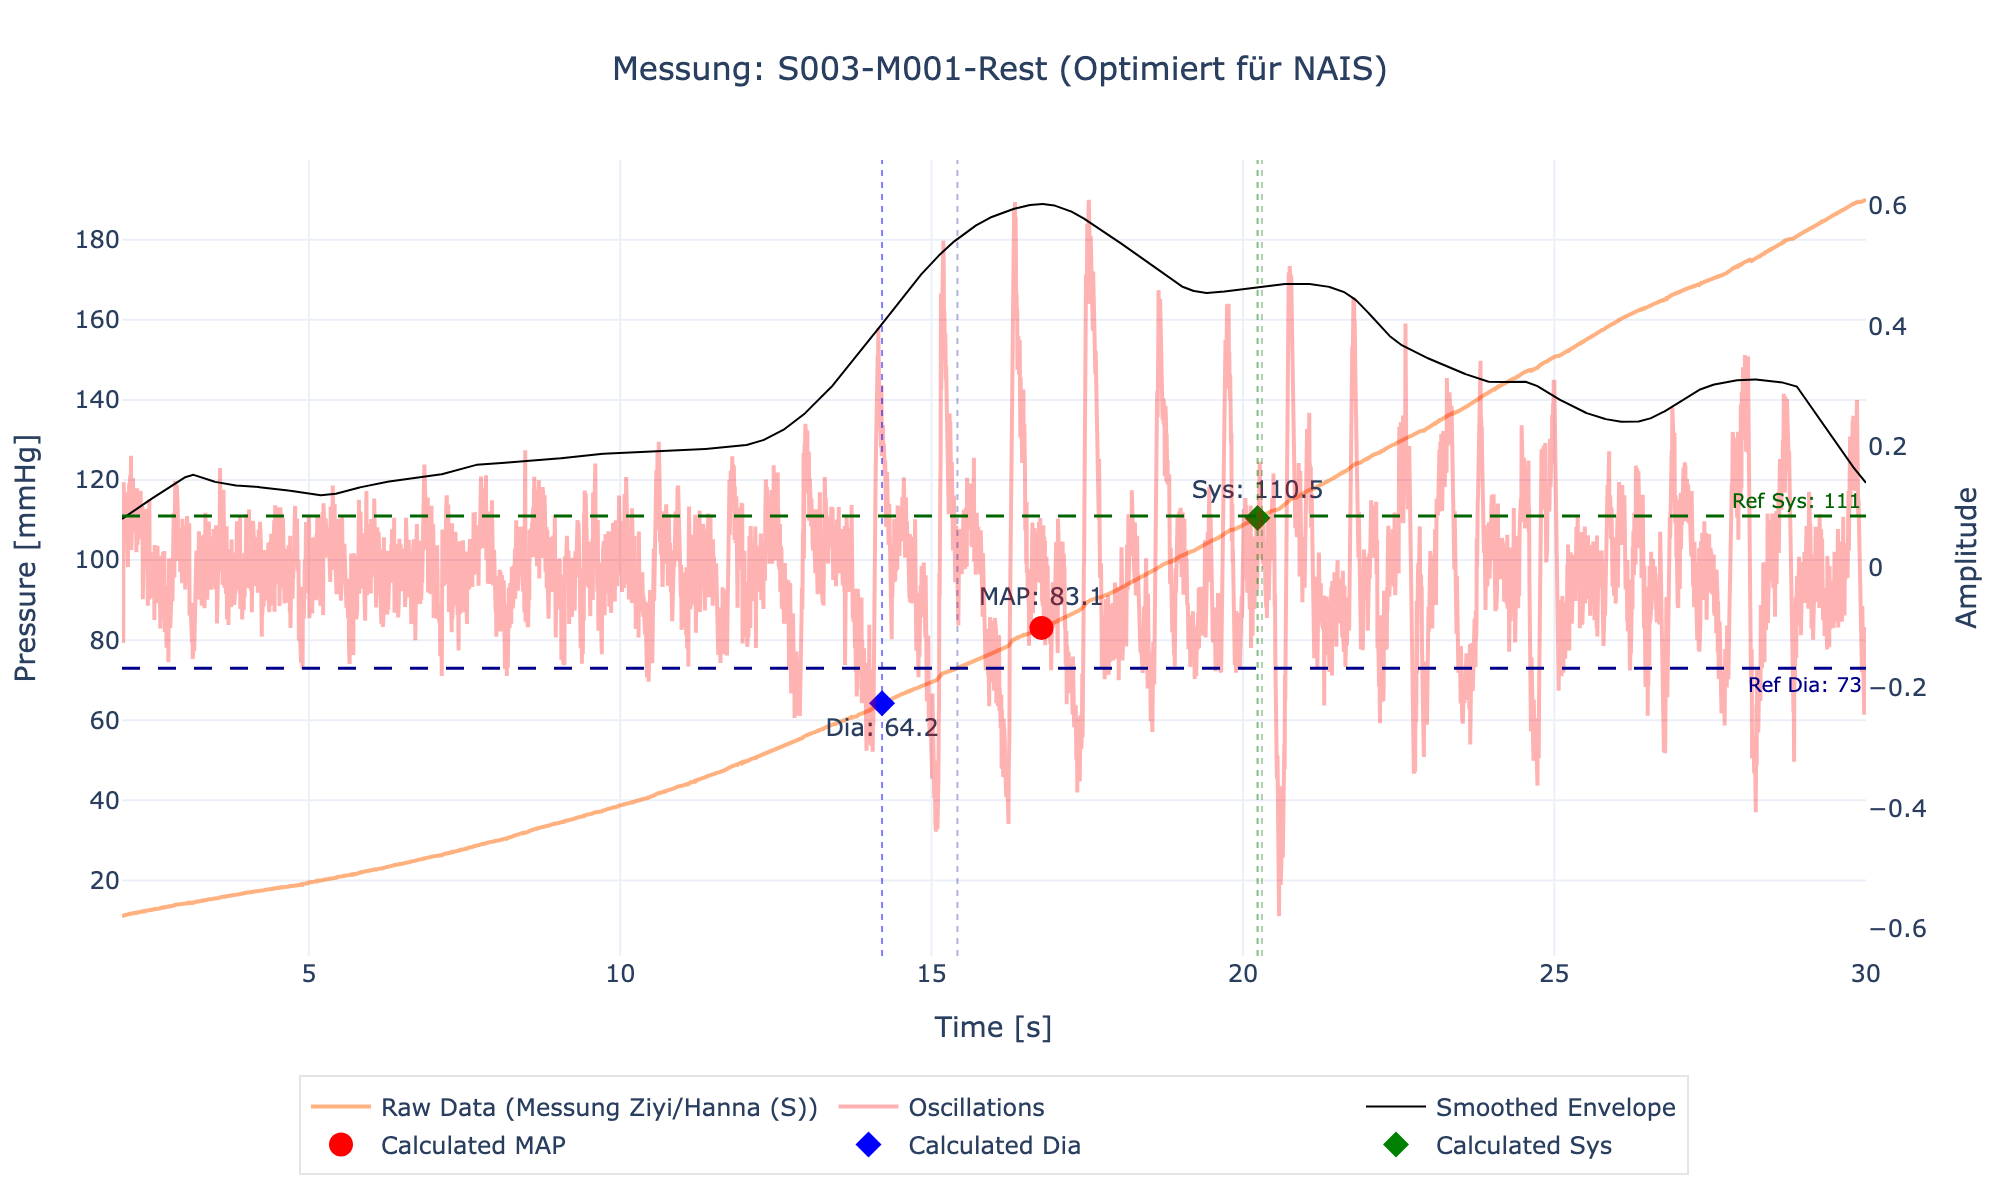
\includegraphics[width=\textwidth]{images/S003-M001-Rest_nais.png}
        \caption{Optimiert für NAIS}
    \end{subfigure}
    \caption{Einzelauswertung der Messung S003-M001-Rest mit verschiedenen Parametersätzen.}
\end{figure}
\newpage

\subsection*{Messung: S003-M002-Active}
\begin{figure}[H]
    \centering
    \begin{subfigure}[b]{0.8\textwidth}
        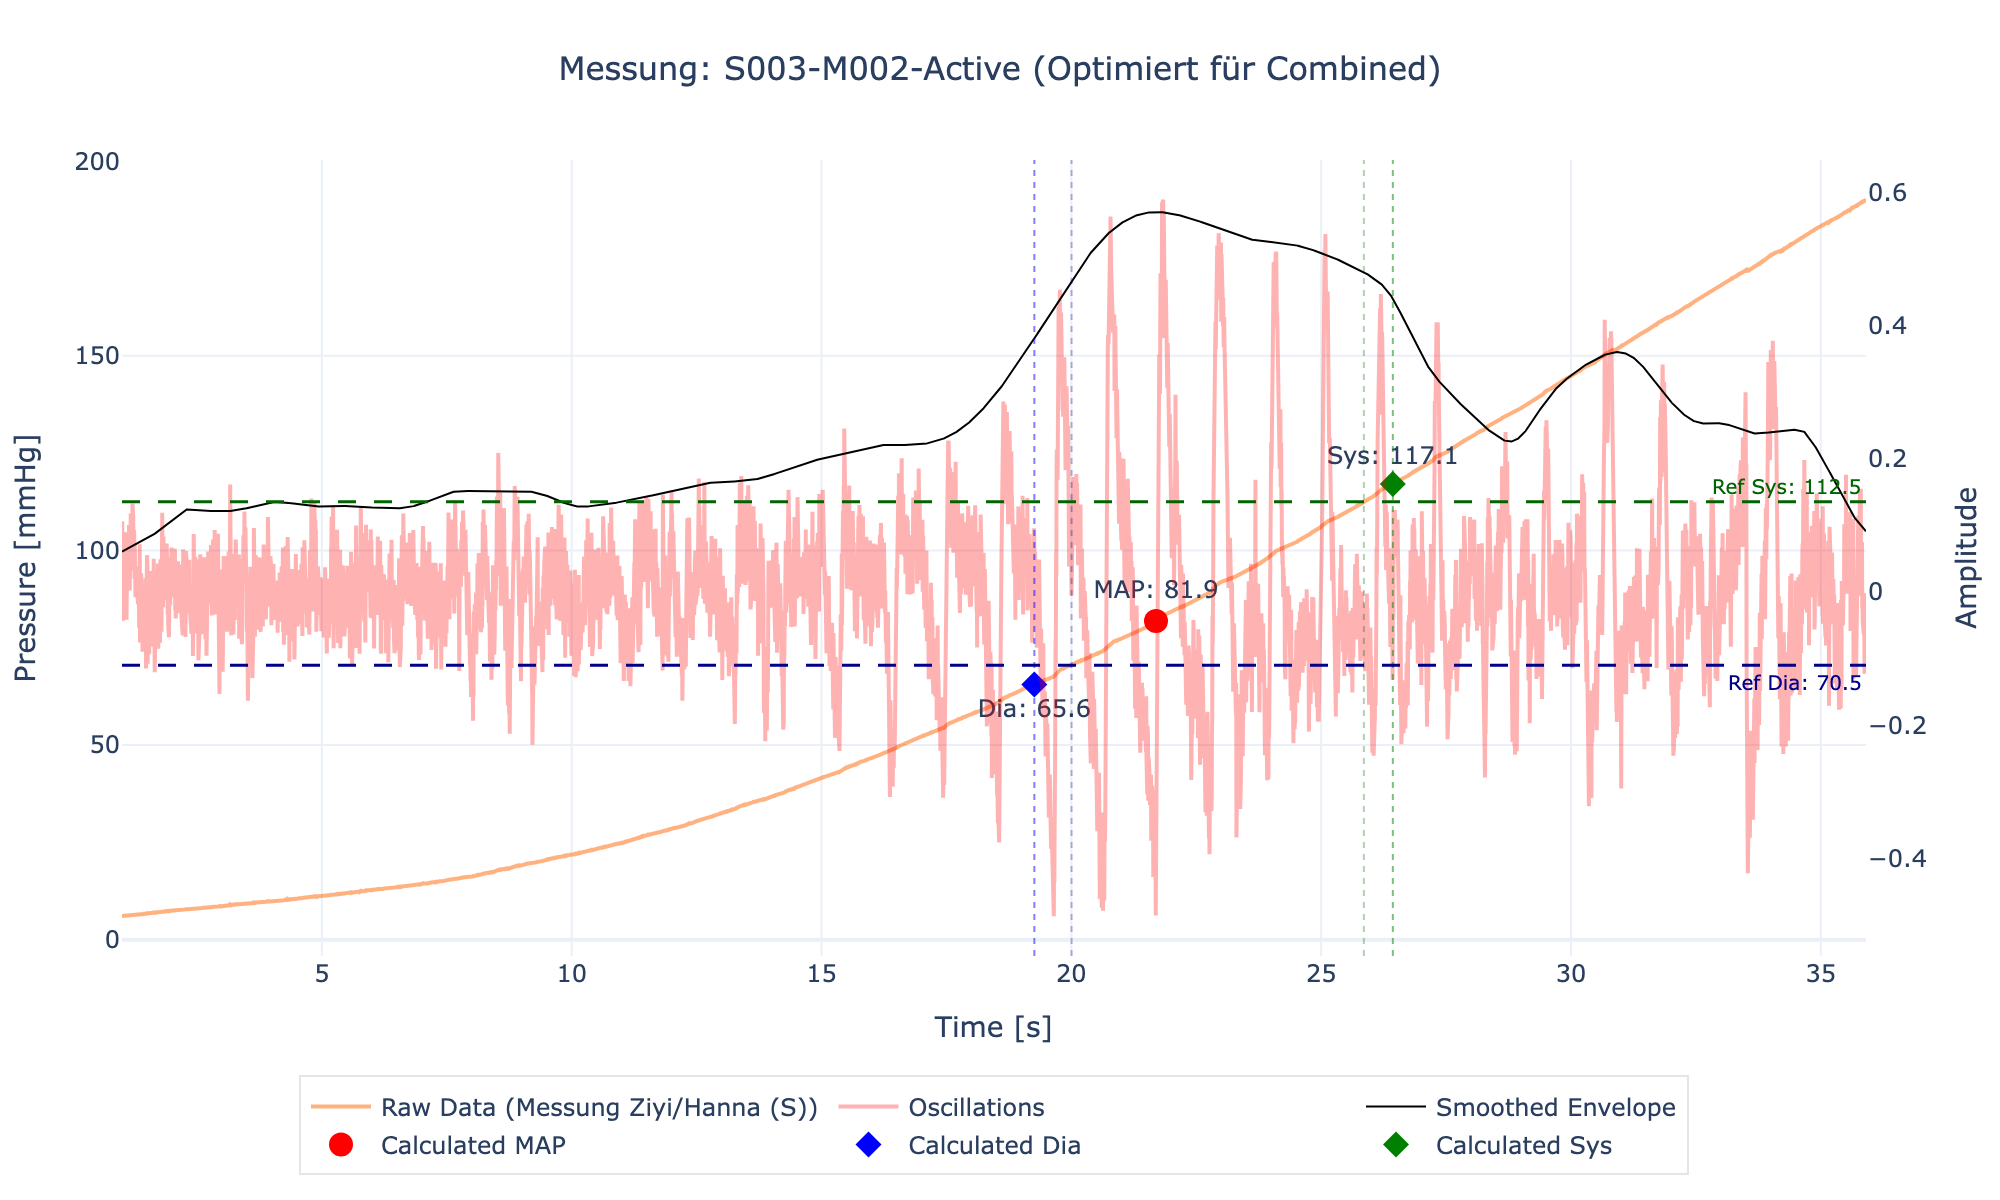
\includegraphics[width=\textwidth]{images/S003-M002-Active_combined.png}
        \caption{Optimiert für Beurer und NAIS (Kombiniert)}
    \end{subfigure} \\
    \begin{subfigure}[b]{0.48\textwidth}
        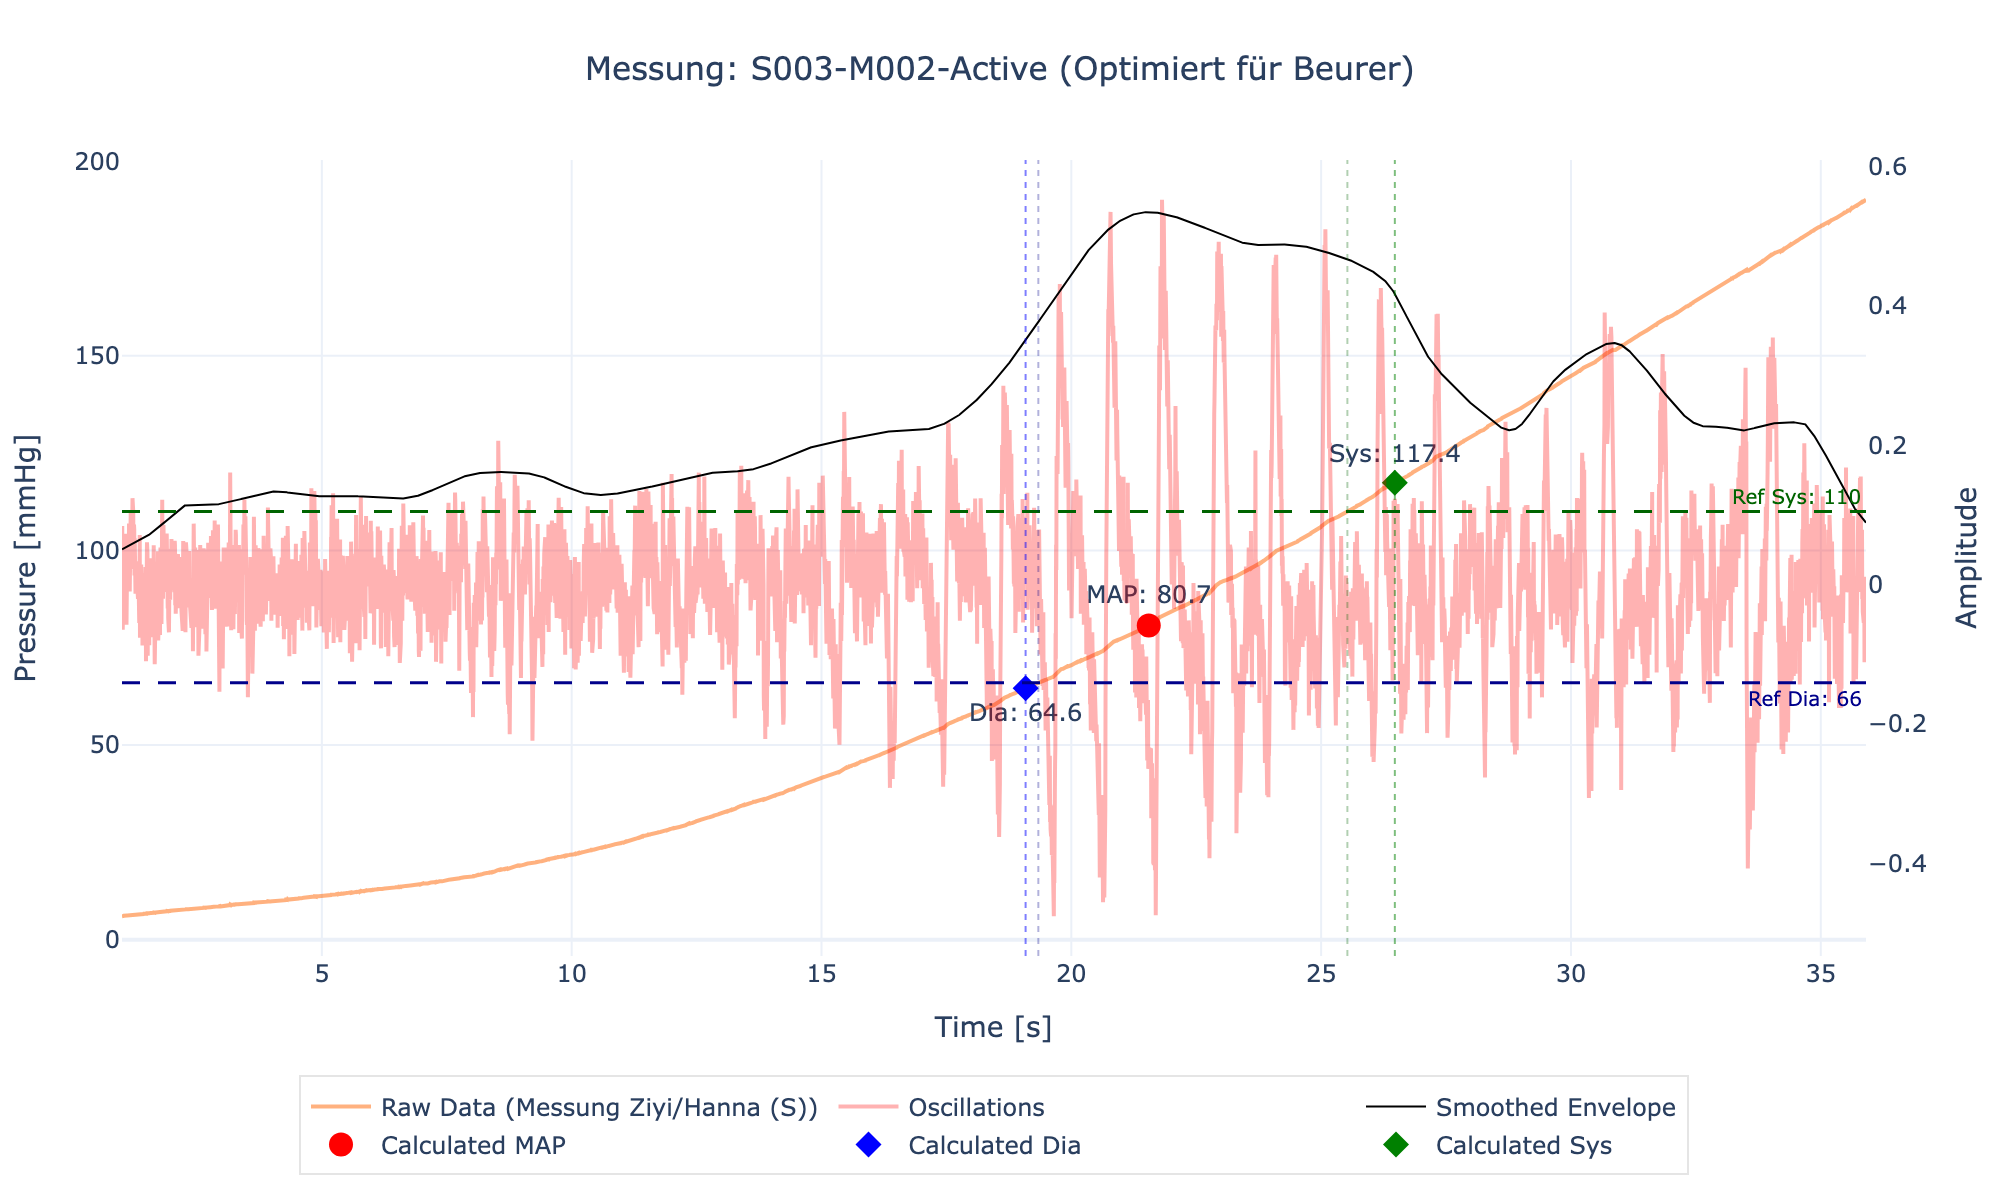
\includegraphics[width=\textwidth]{images/S003-M002-Active_beurer.png}
        \caption{Optimiert für Beurer}
    \end{subfigure}
    \hfill
    \begin{subfigure}[b]{0.48\textwidth}
        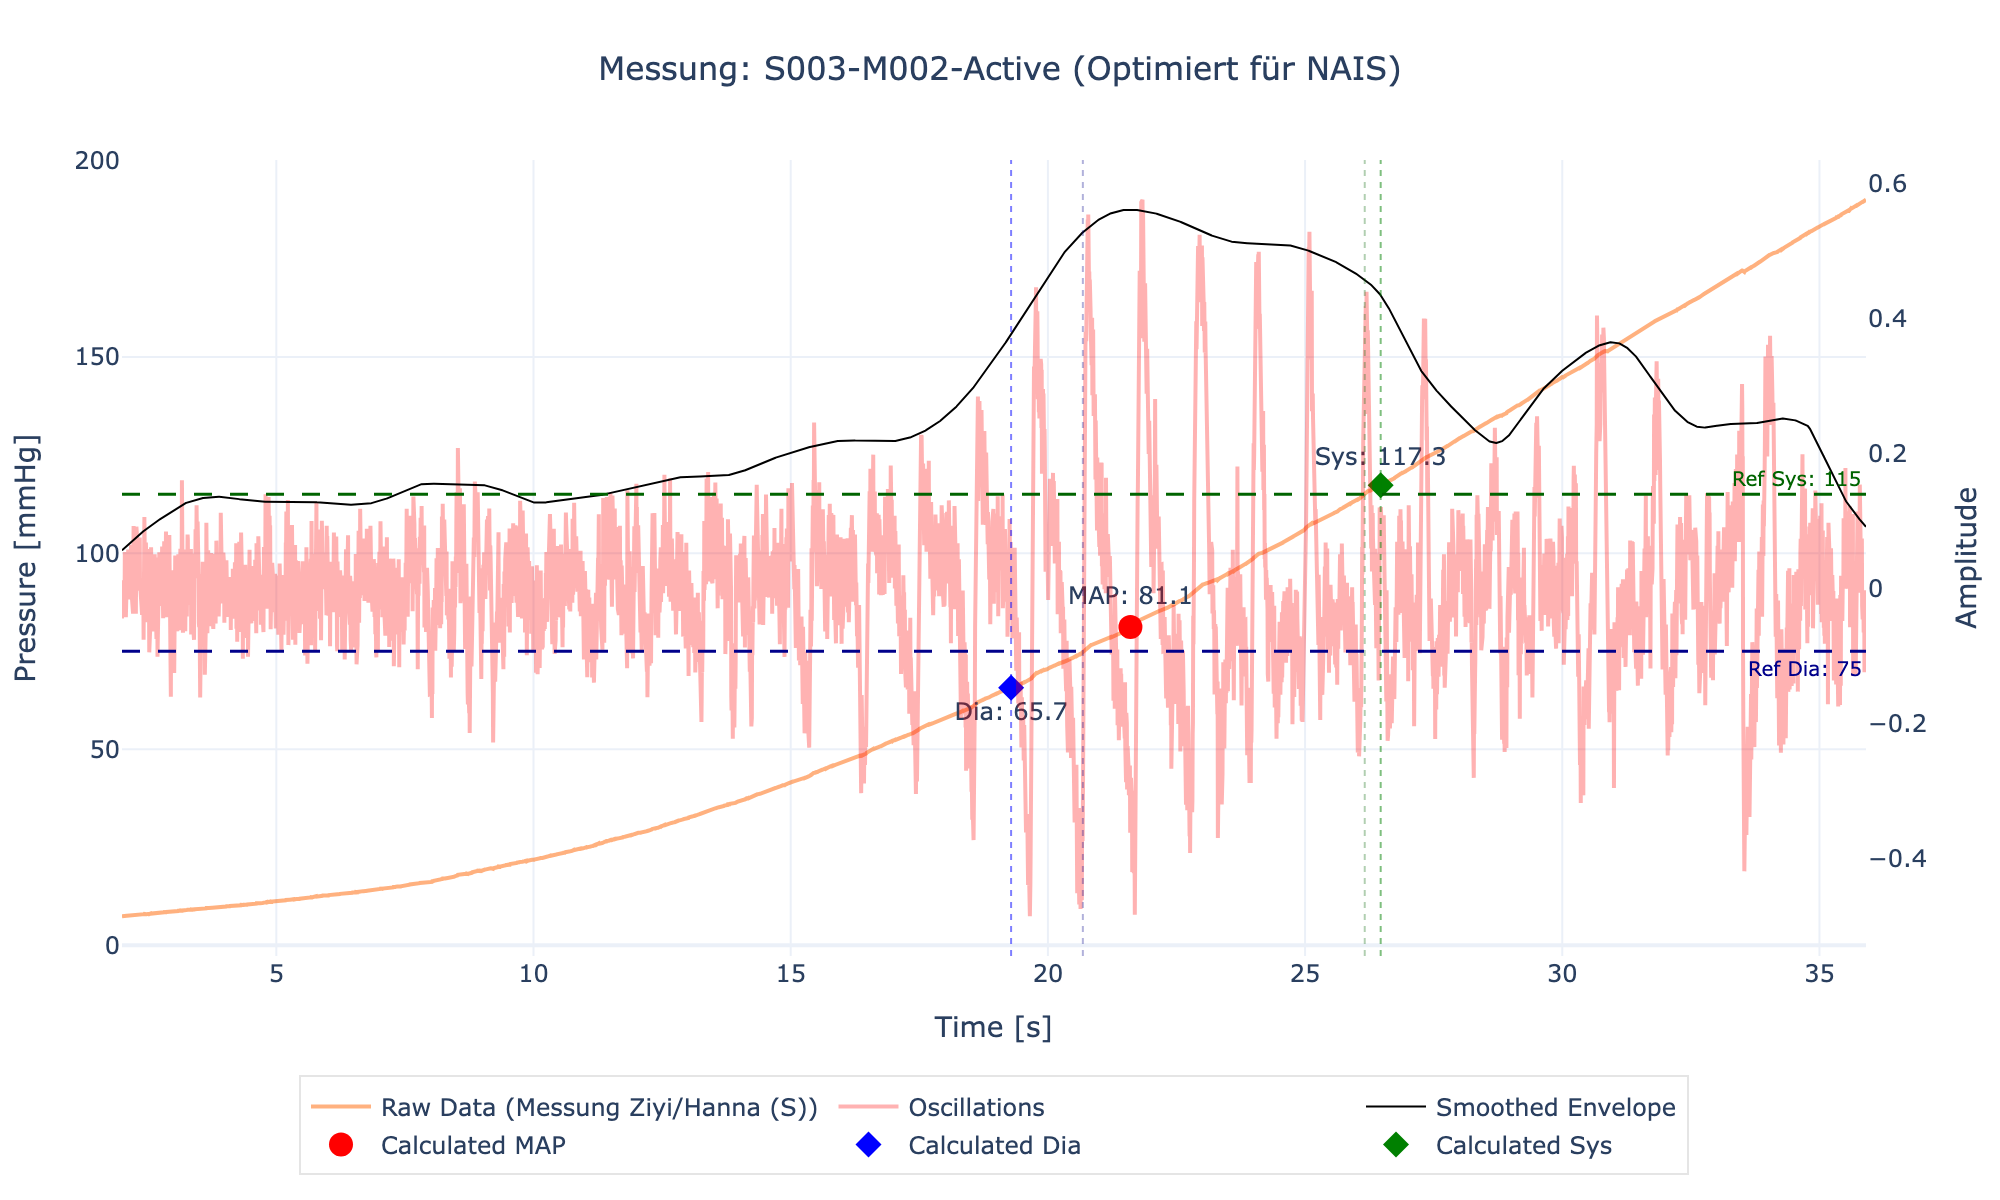
\includegraphics[width=\textwidth]{images/S003-M002-Active_nais.png}
        \caption{Optimiert für NAIS}
    \end{subfigure}
    \caption{Einzelauswertung der Messung S003-M002-Active mit verschiedenen Parametersätzen.}
\end{figure}
\newpage

\subsection*{Messung: S004-M001-Rest}
\begin{figure}[H]
    \centering
    \begin{subfigure}[b]{0.8\textwidth}
        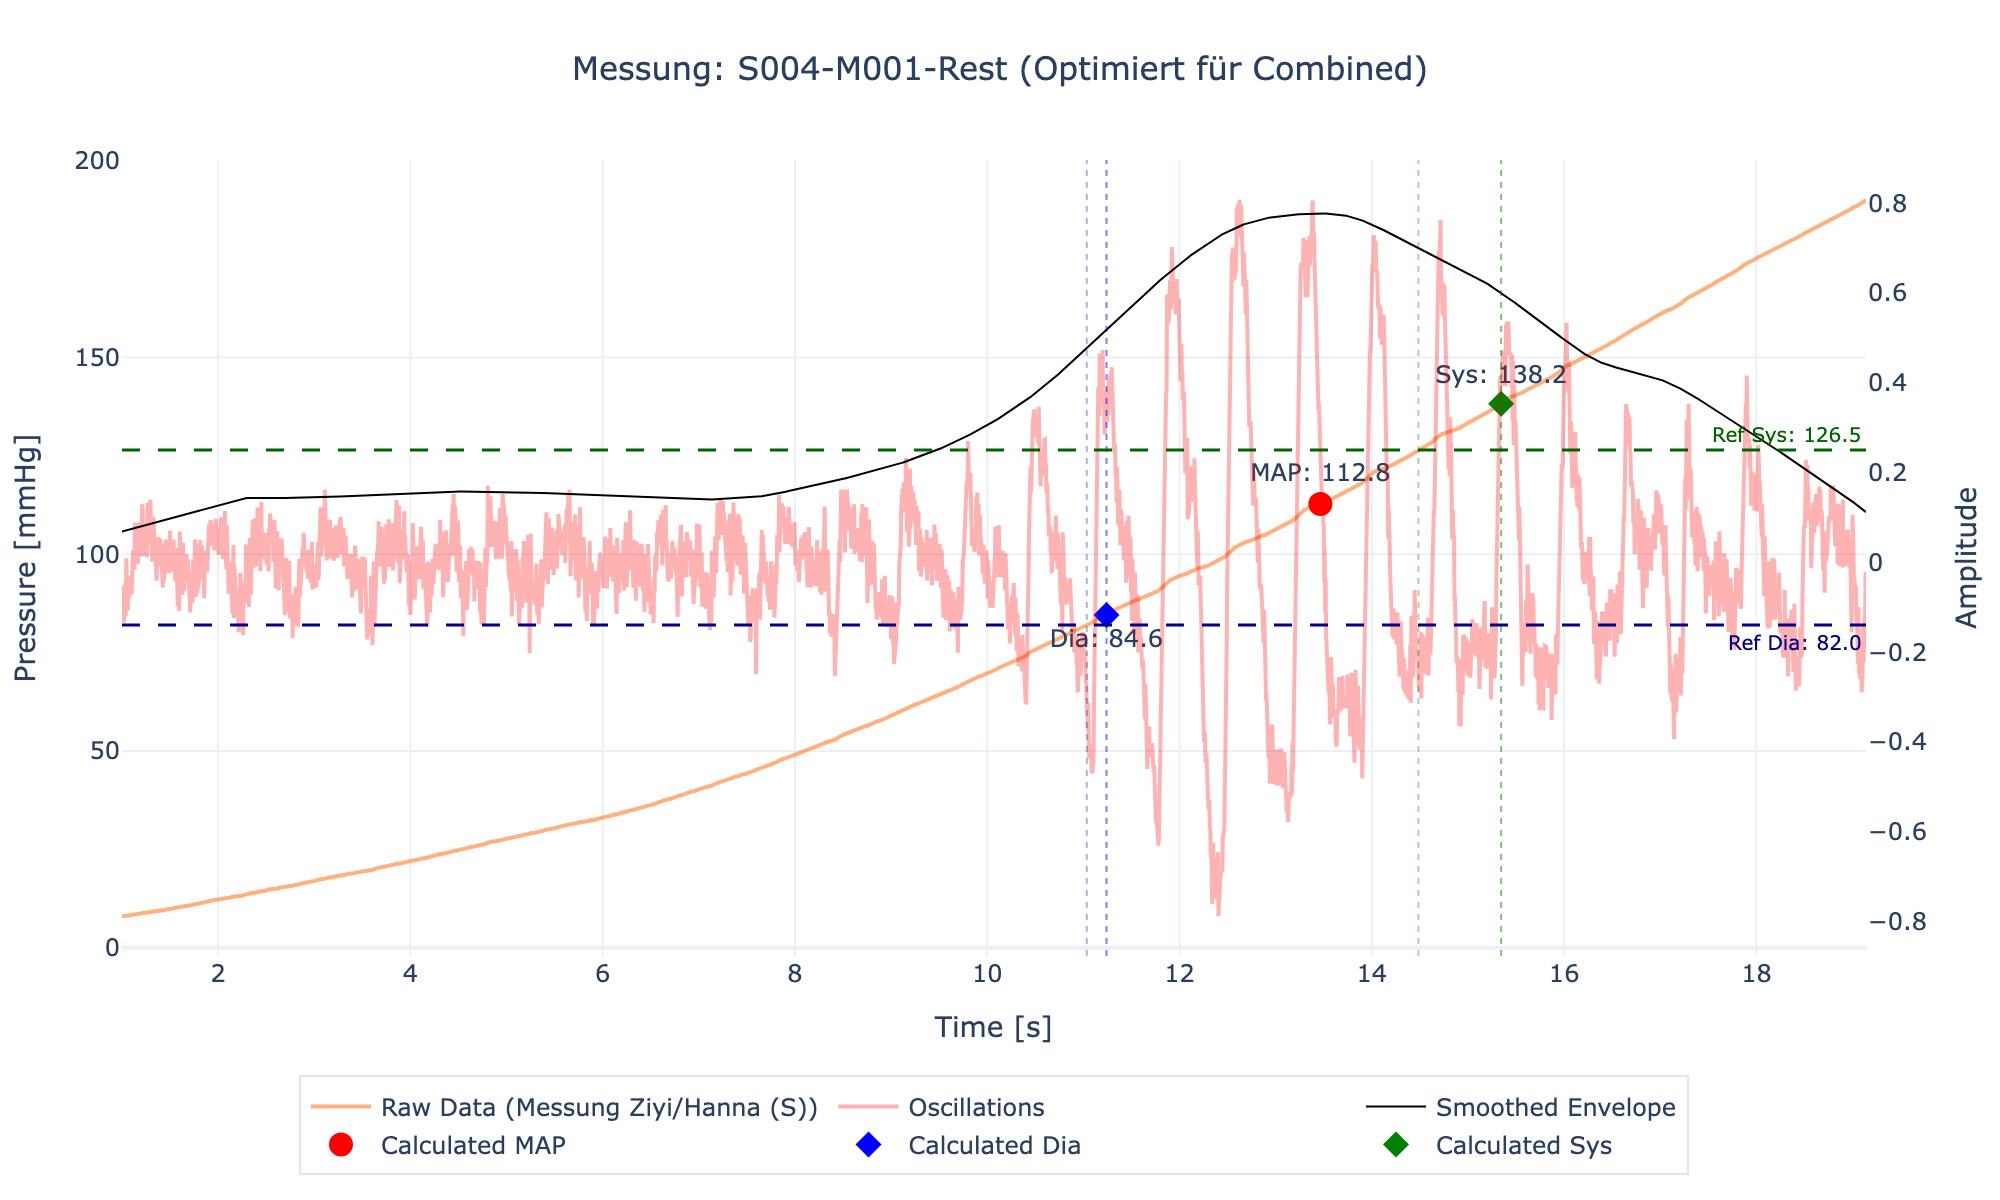
\includegraphics[width=\textwidth]{images/S004-M001-Rest_combined.png}
        \caption{Optimiert für Beurer und NAIS (Kombiniert)}
    \end{subfigure} \\
    \begin{subfigure}[b]{0.48\textwidth}
        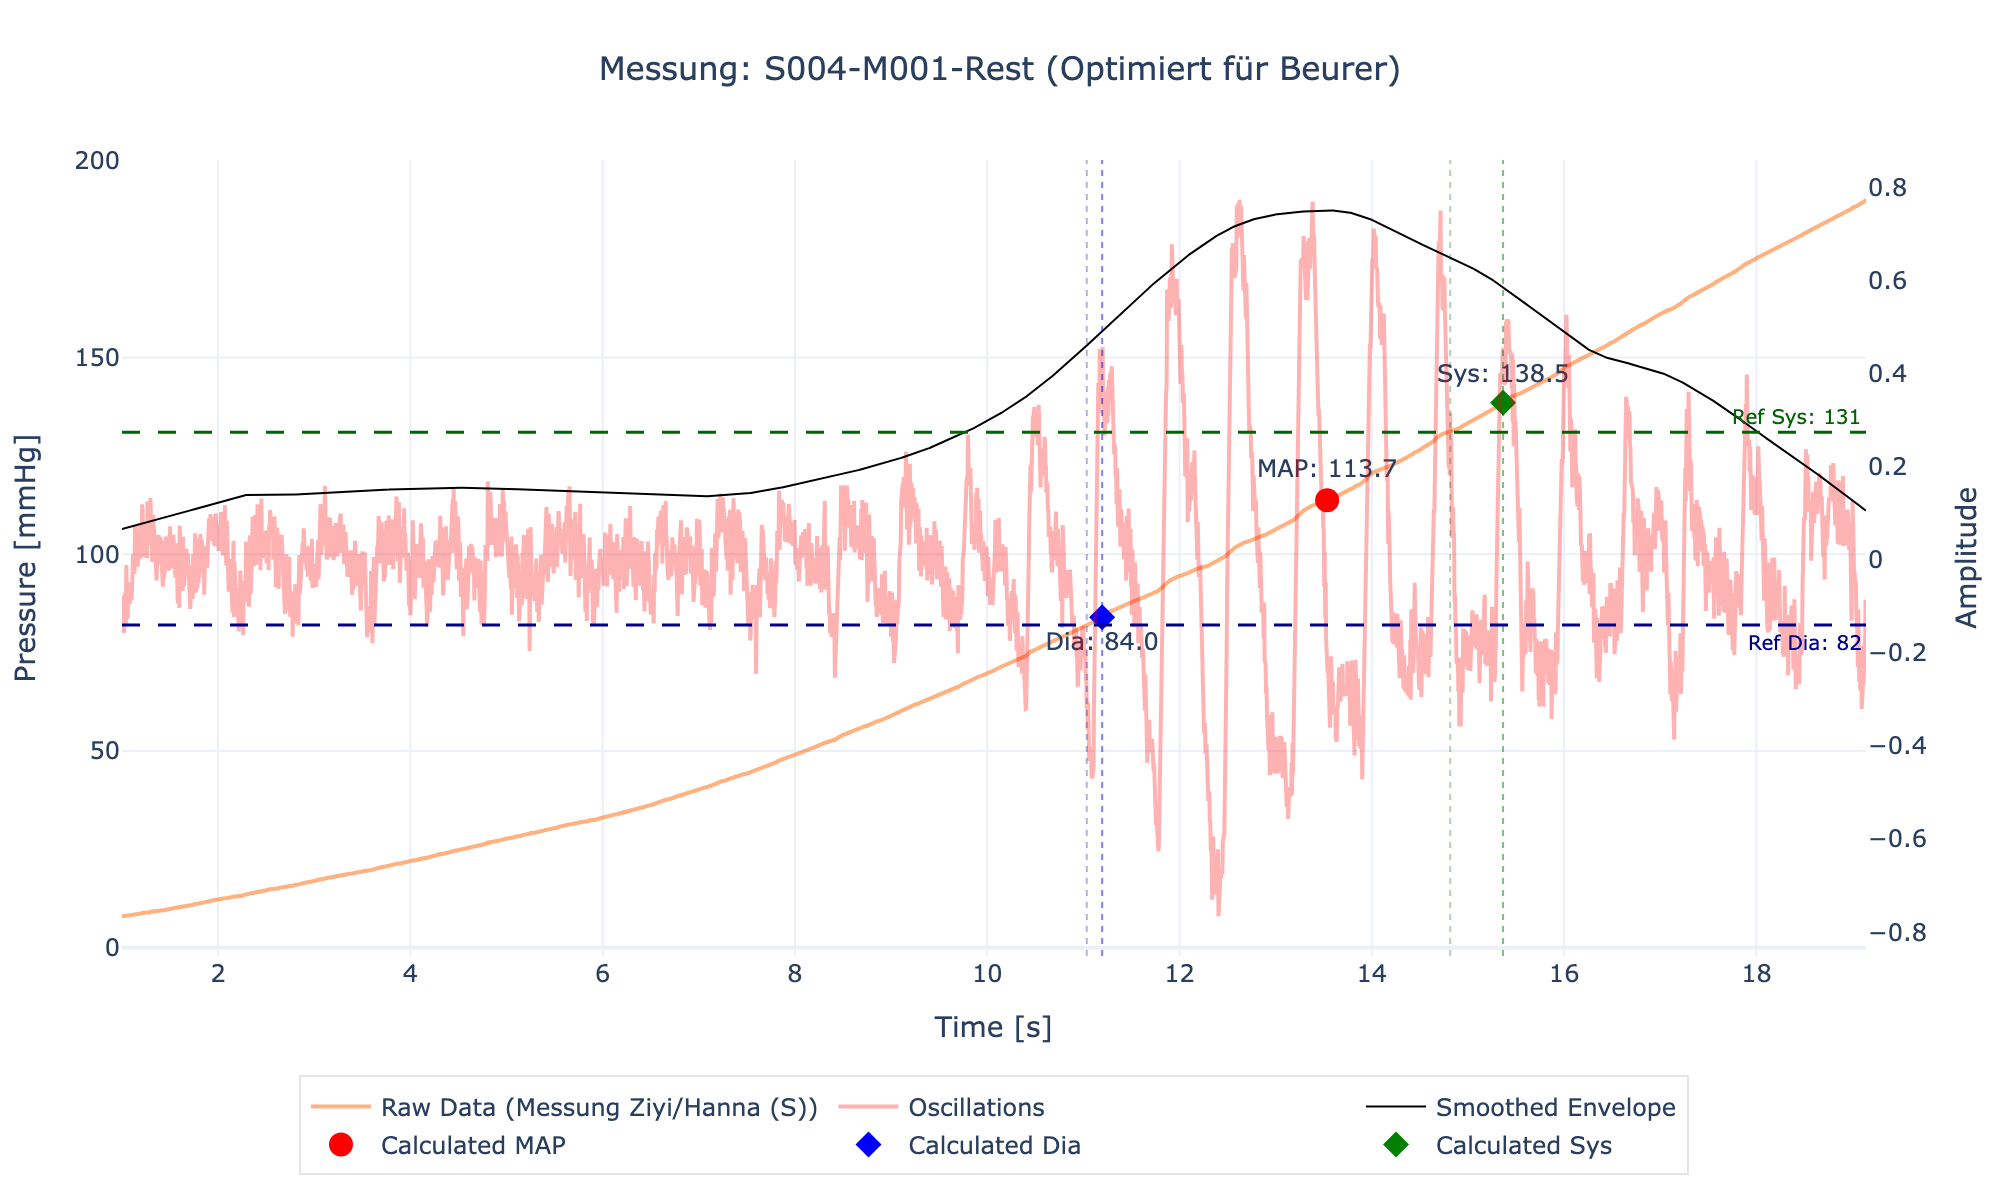
\includegraphics[width=\textwidth]{images/S004-M001-Rest_beurer.png}
        \caption{Optimiert für Beurer}
    \end{subfigure}
    \hfill
    \begin{subfigure}[b]{0.48\textwidth}
        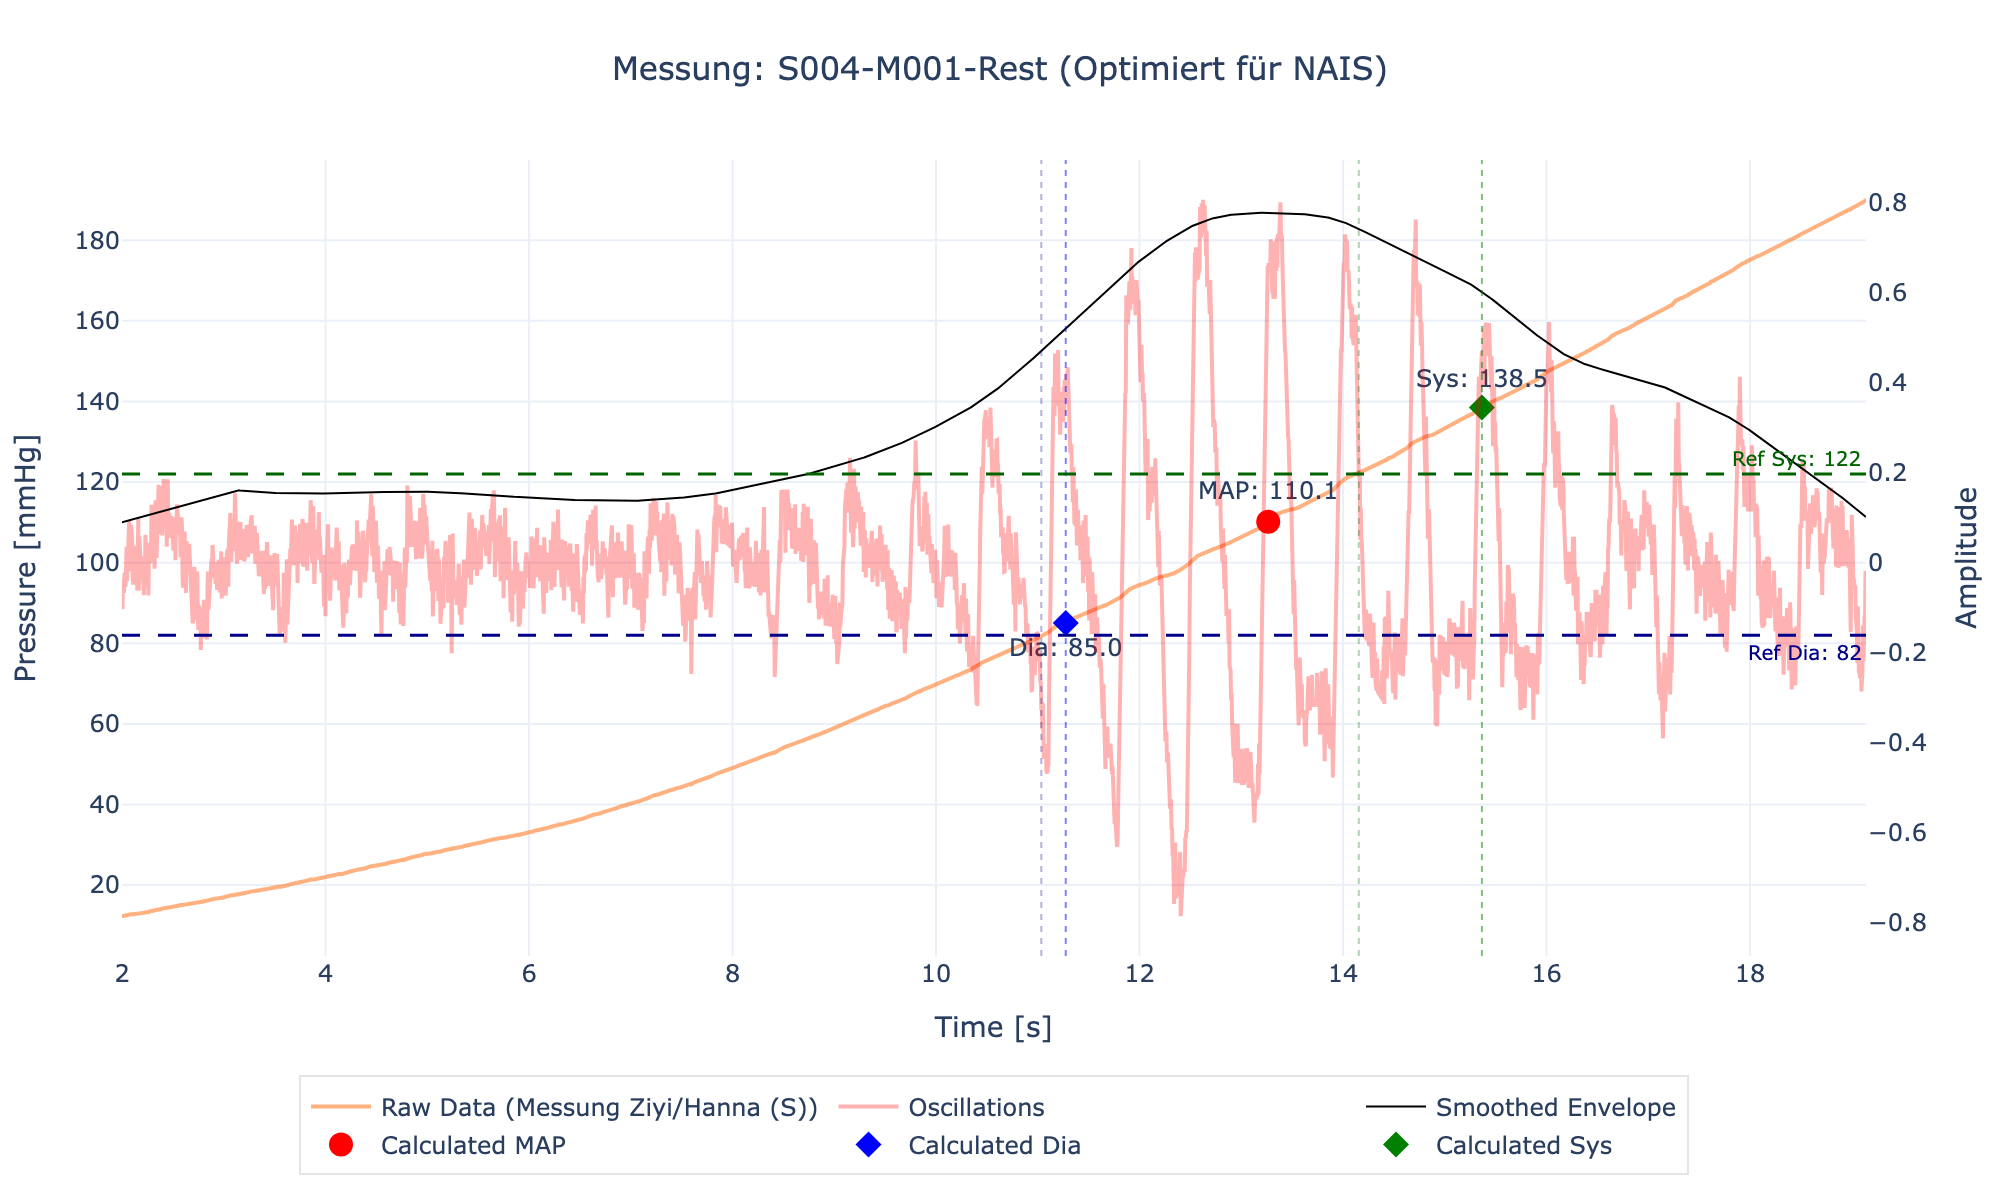
\includegraphics[width=\textwidth]{images/S004-M001-Rest_nais.png}
        \caption{Optimiert für NAIS}
    \end{subfigure}
    \caption{Einzelauswertung der Messung S004-M001-Rest mit verschiedenen Parametersätzen.}
\end{figure}
\newpage

\subsection*{Messung: S004-M002-Active}
\begin{figure}[H]
    \centering
    \begin{subfigure}[b]{0.8\textwidth}
        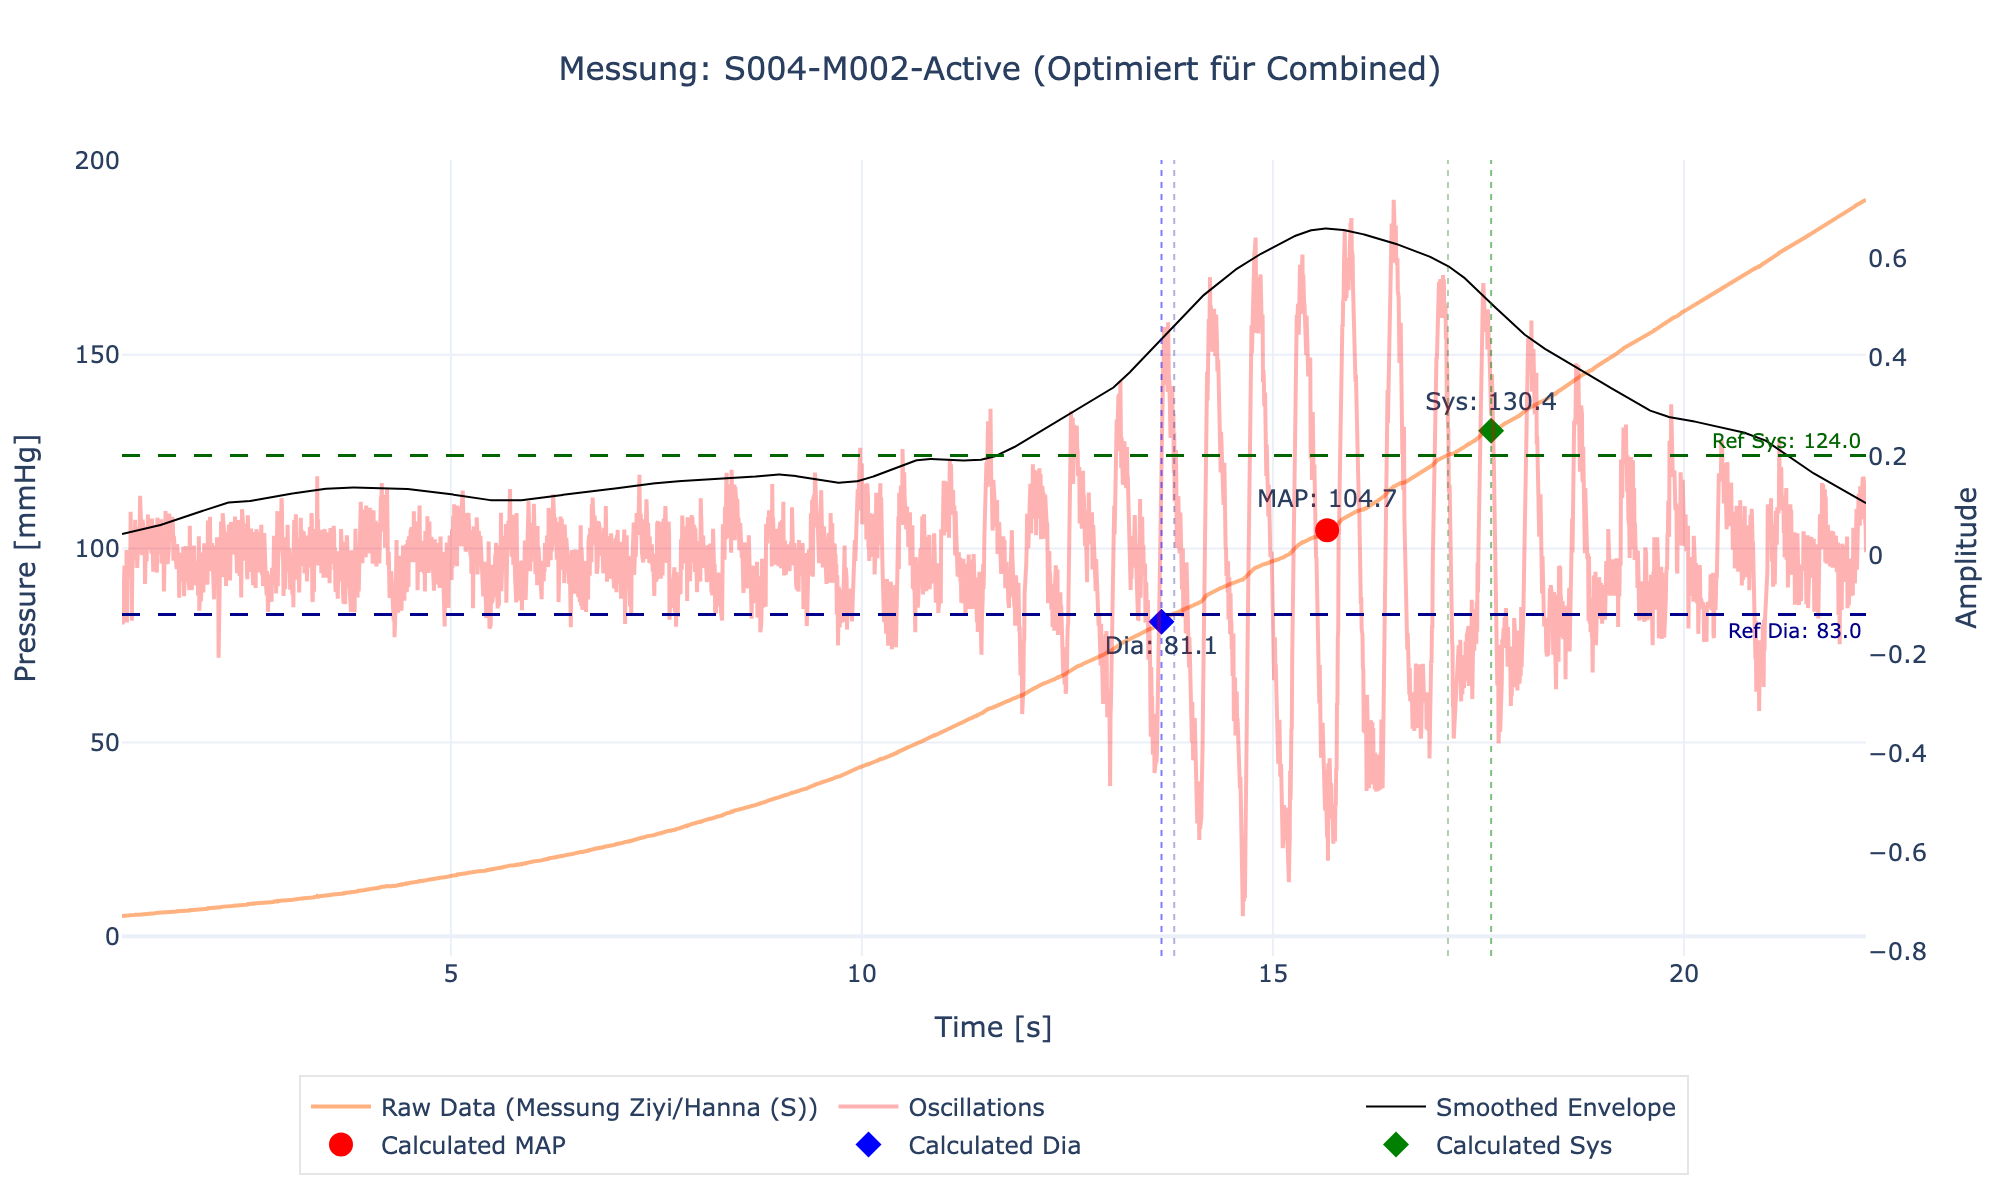
\includegraphics[width=\textwidth]{images/S004-M002-Active_combined.png}
        \caption{Optimiert für Beurer und NAIS (Kombiniert)}
    \end{subfigure} \\
    \begin{subfigure}[b]{0.48\textwidth}
        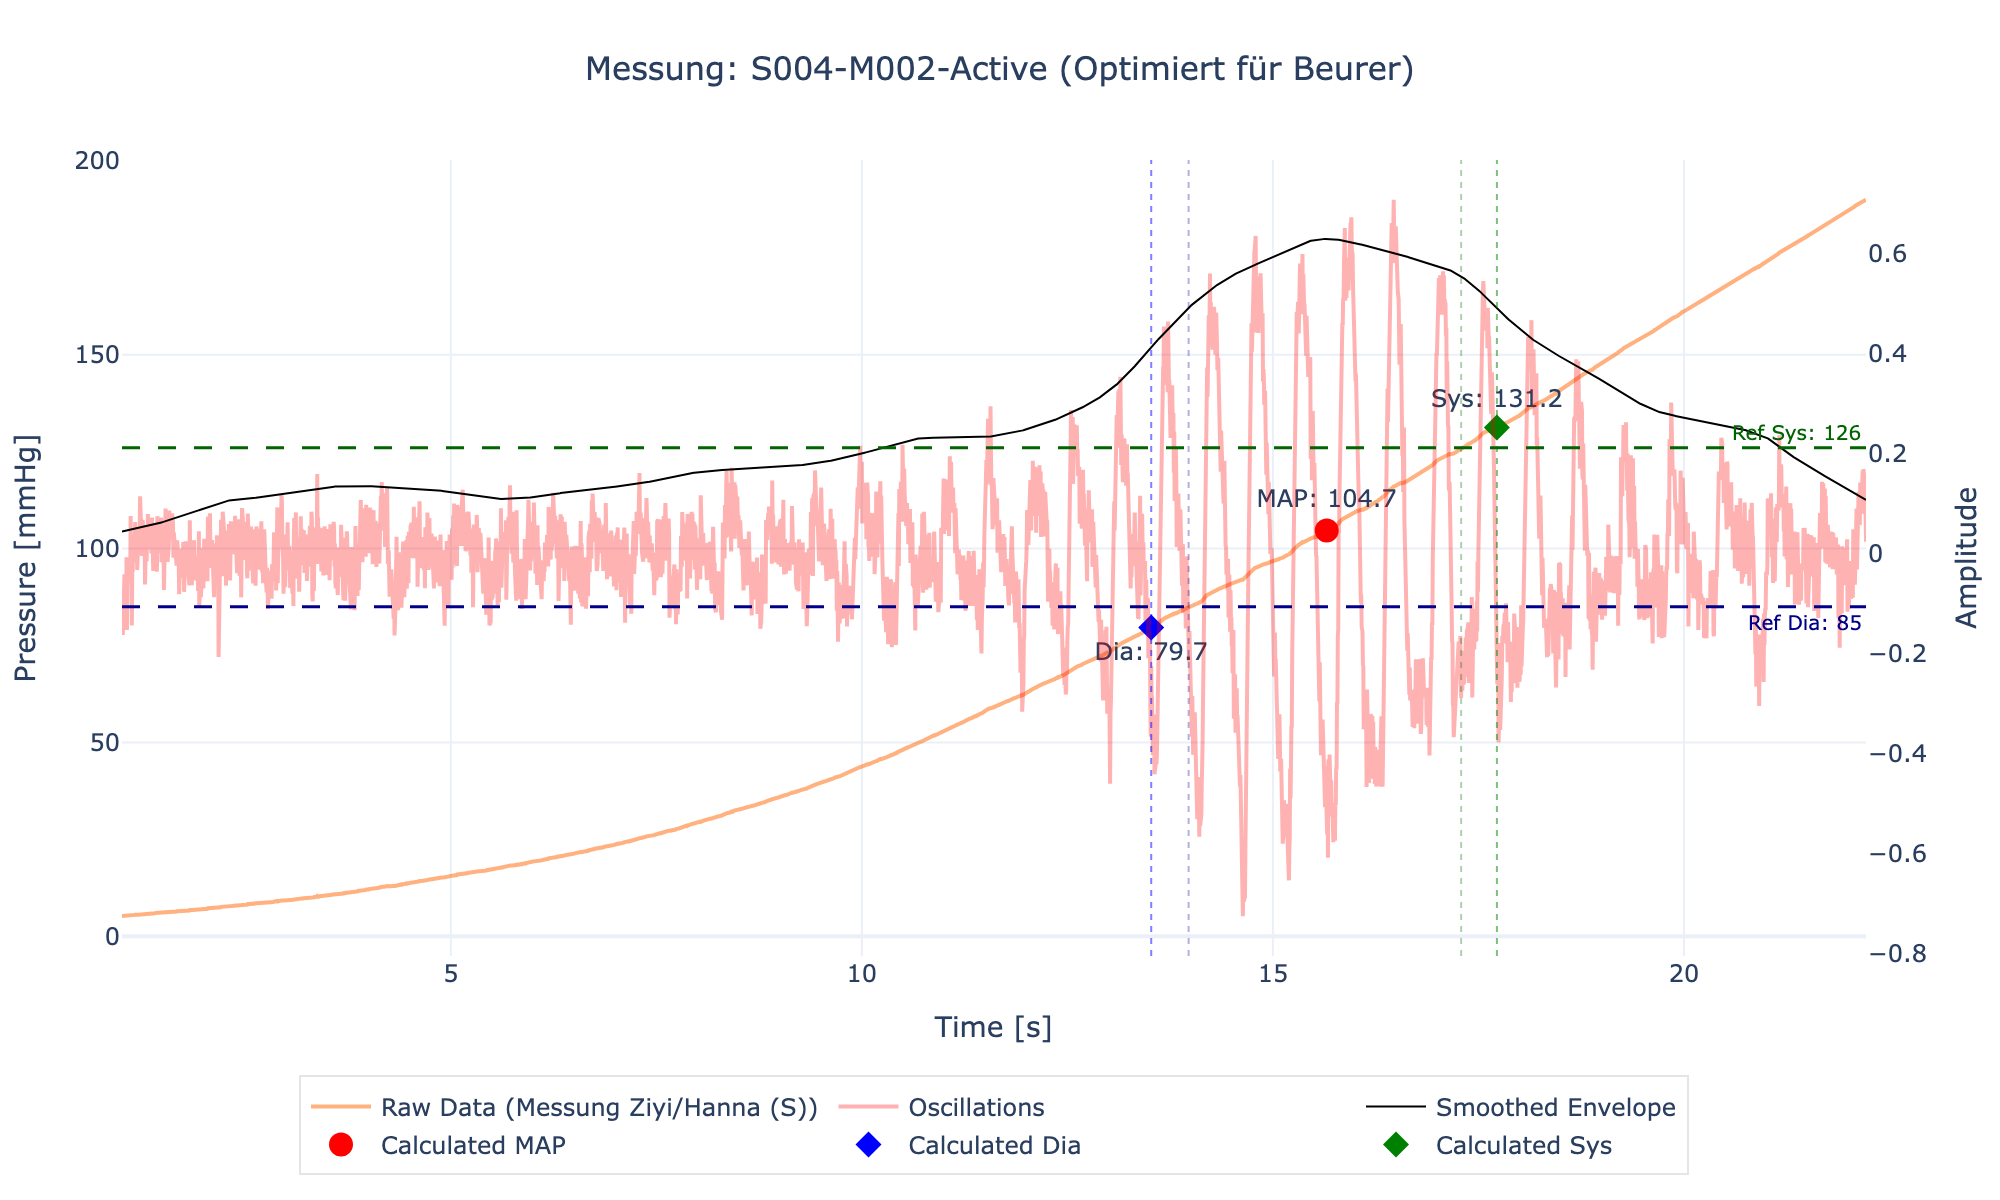
\includegraphics[width=\textwidth]{images/S004-M002-Active_beurer.png}
        \caption{Optimiert für Beurer}
    \end{subfigure}
    \hfill
    \begin{subfigure}[b]{0.48\textwidth}
        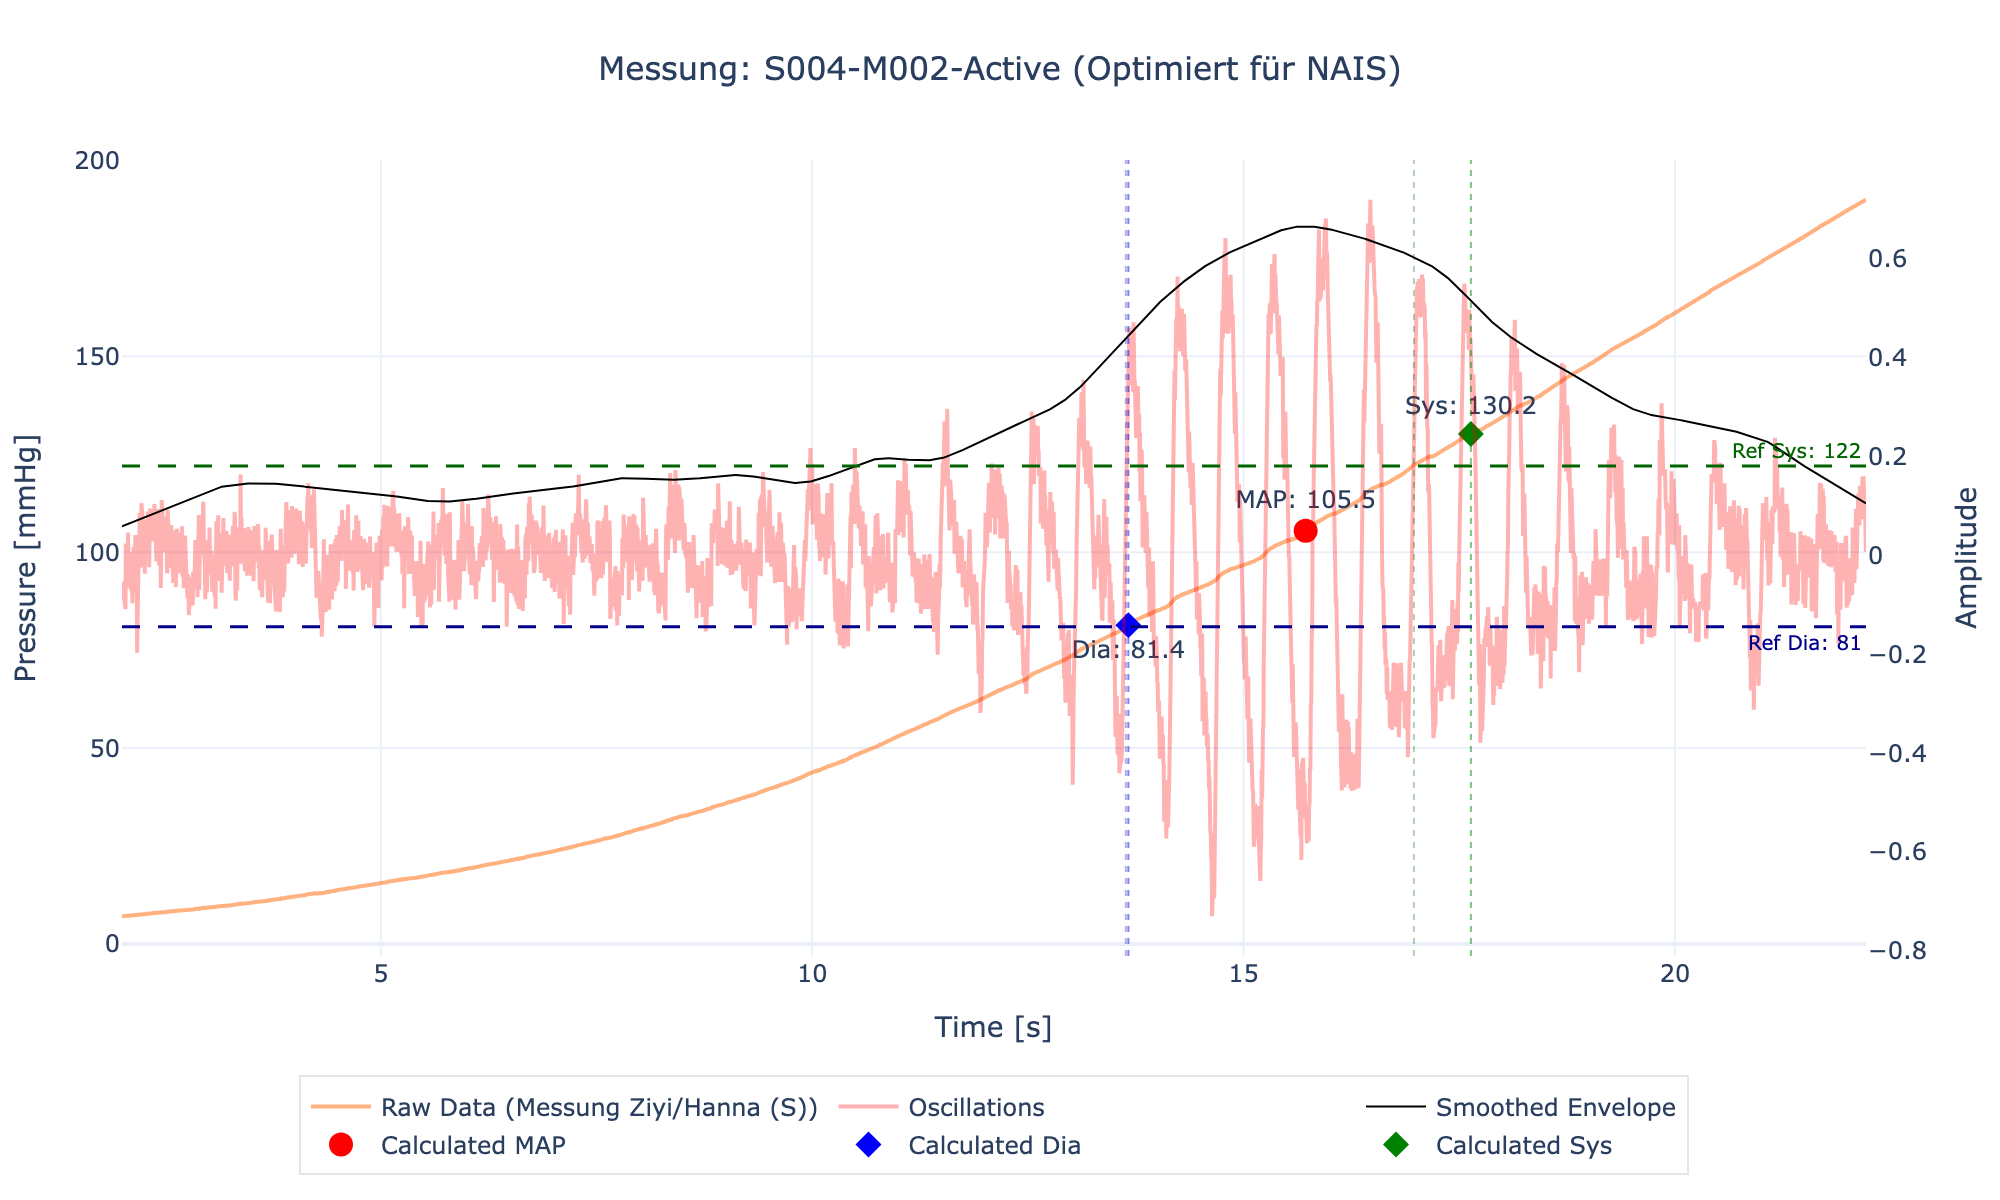
\includegraphics[width=\textwidth]{images/S004-M002-Active_nais.png}
        \caption{Optimiert für NAIS}
    \end{subfigure}
    \caption{Einzelauswertung der Messung S004-M002-Active mit verschiedenen Parametersätzen.}
\end{figure}
\newpage

\subsection*{Messung: S005-M001-Rest}
\begin{figure}[H]
    \centering
    \begin{subfigure}[b]{0.8\textwidth}
        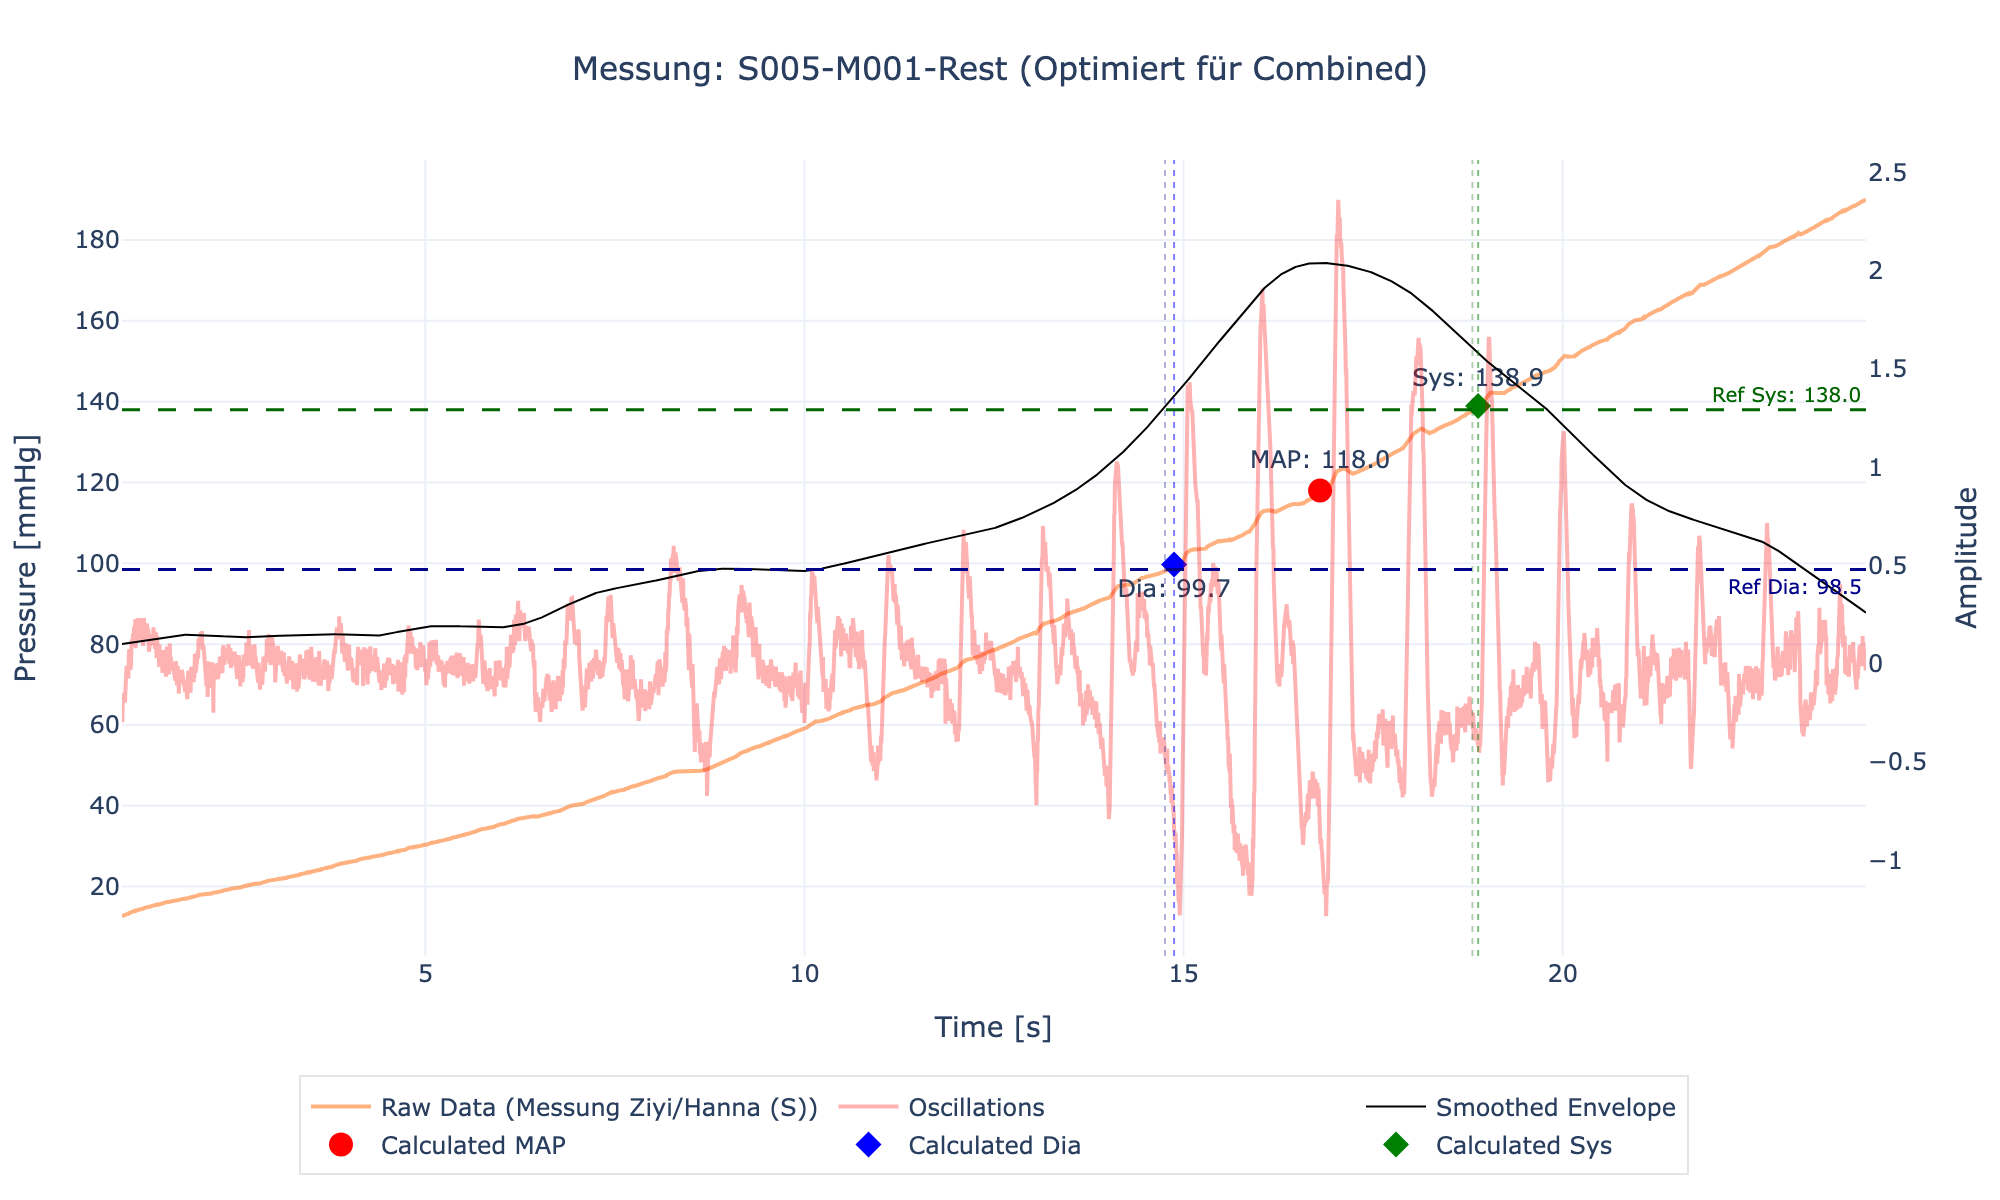
\includegraphics[width=\textwidth]{images/S005-M001-Rest_combined.png}
        \caption{Optimiert für Beurer und NAIS (Kombiniert)}
    \end{subfigure} \\
    \begin{subfigure}[b]{0.48\textwidth}
        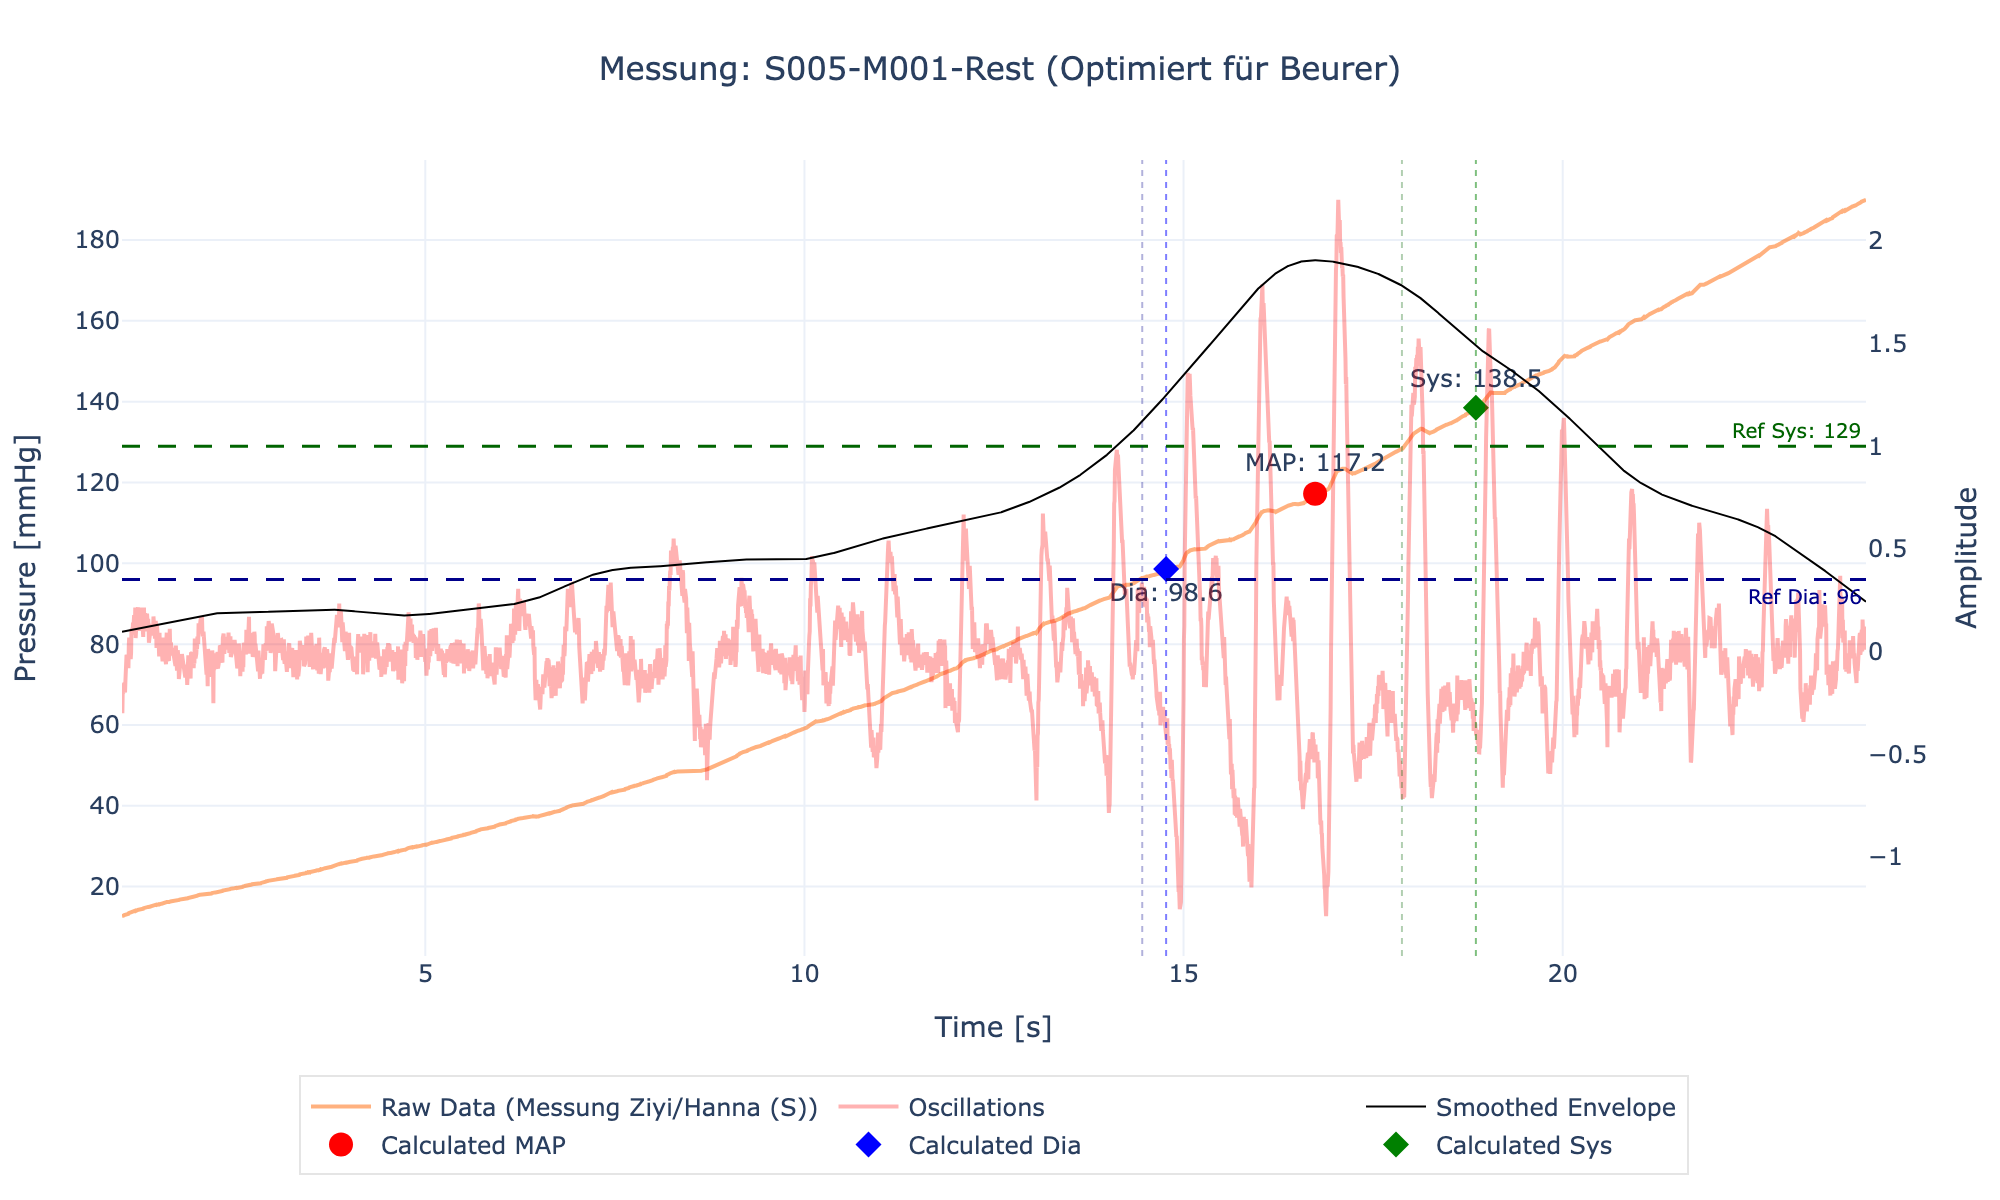
\includegraphics[width=\textwidth]{images/S005-M001-Rest_beurer.png}
        \caption{Optimiert für Beurer}
    \end{subfigure}
    \hfill
    \begin{subfigure}[b]{0.48\textwidth}
        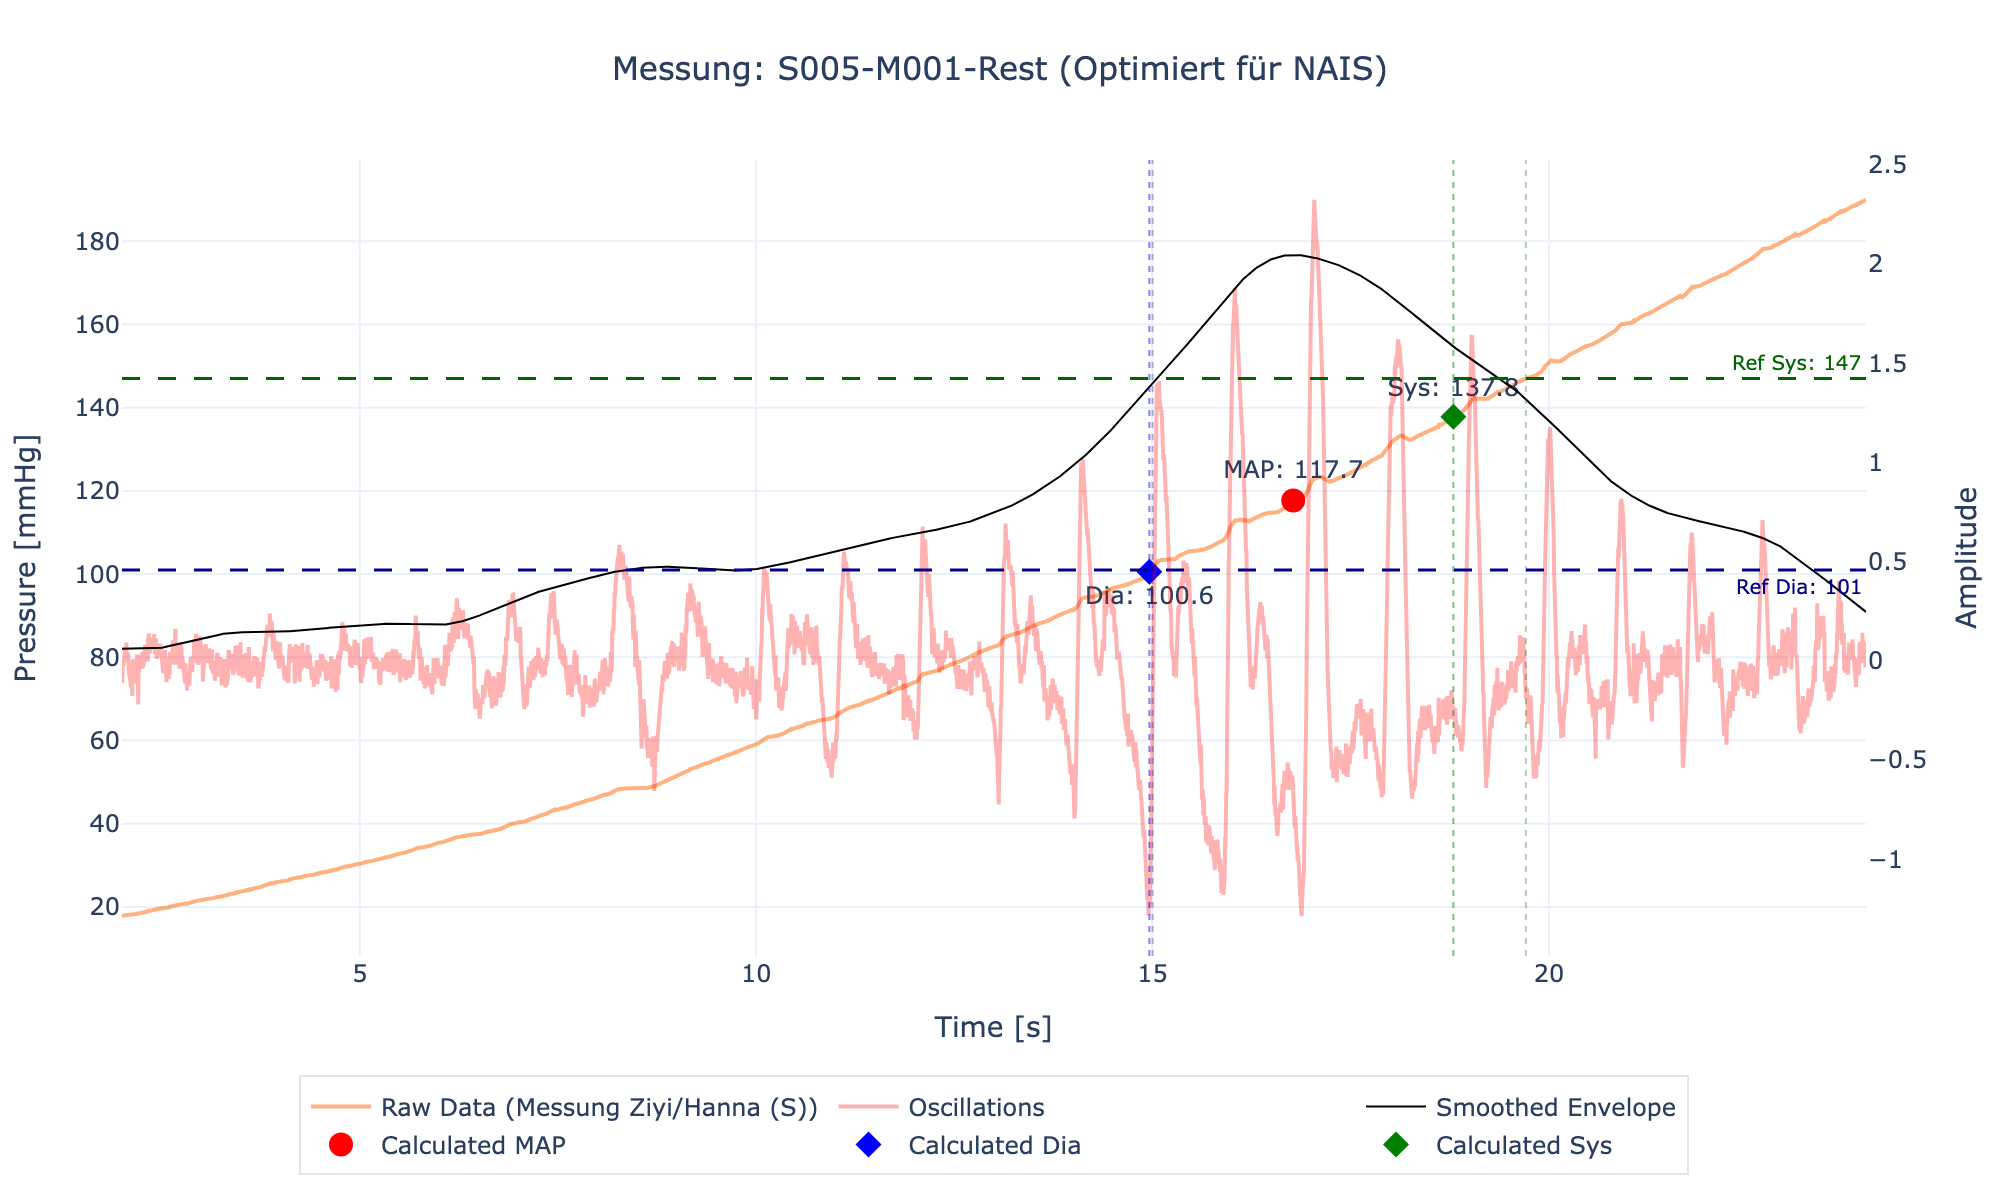
\includegraphics[width=\textwidth]{images/S005-M001-Rest_nais.png}
        \caption{Optimiert für NAIS}
    \end{subfigure}
    \caption{Einzelauswertung der Messung S005-M001-Rest mit verschiedenen Parametersätzen.}
\end{figure}
\newpage

\subsection*{Messung: S005-M002-Active}
\begin{figure}[H]
    \centering
    \begin{subfigure}[b]{0.8\textwidth}
        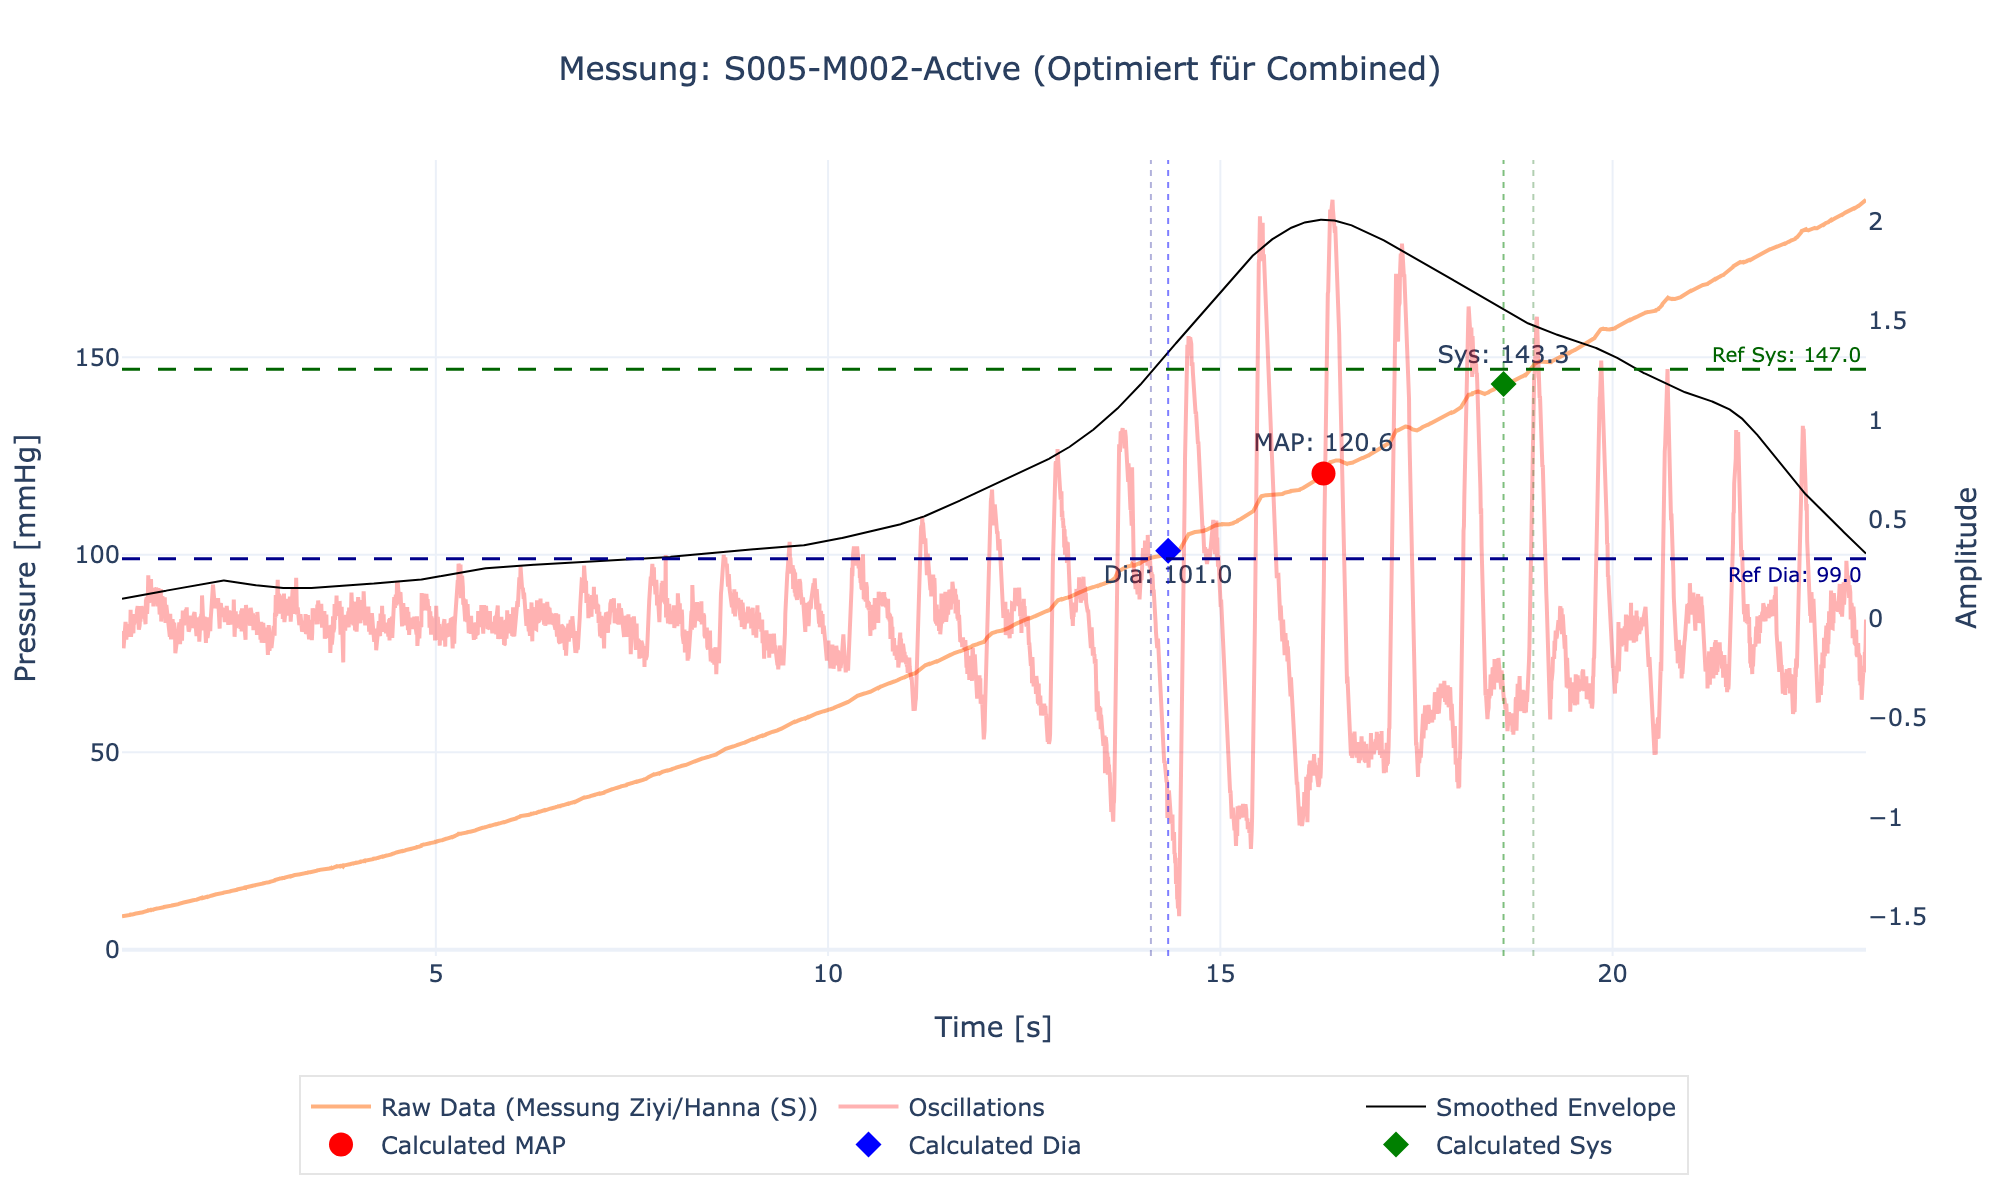
\includegraphics[width=\textwidth]{images/S005-M002-Active_combined.png}
        \caption{Optimiert für Beurer und NAIS (Kombiniert)}
    \end{subfigure} \\
    \begin{subfigure}[b]{0.48\textwidth}
        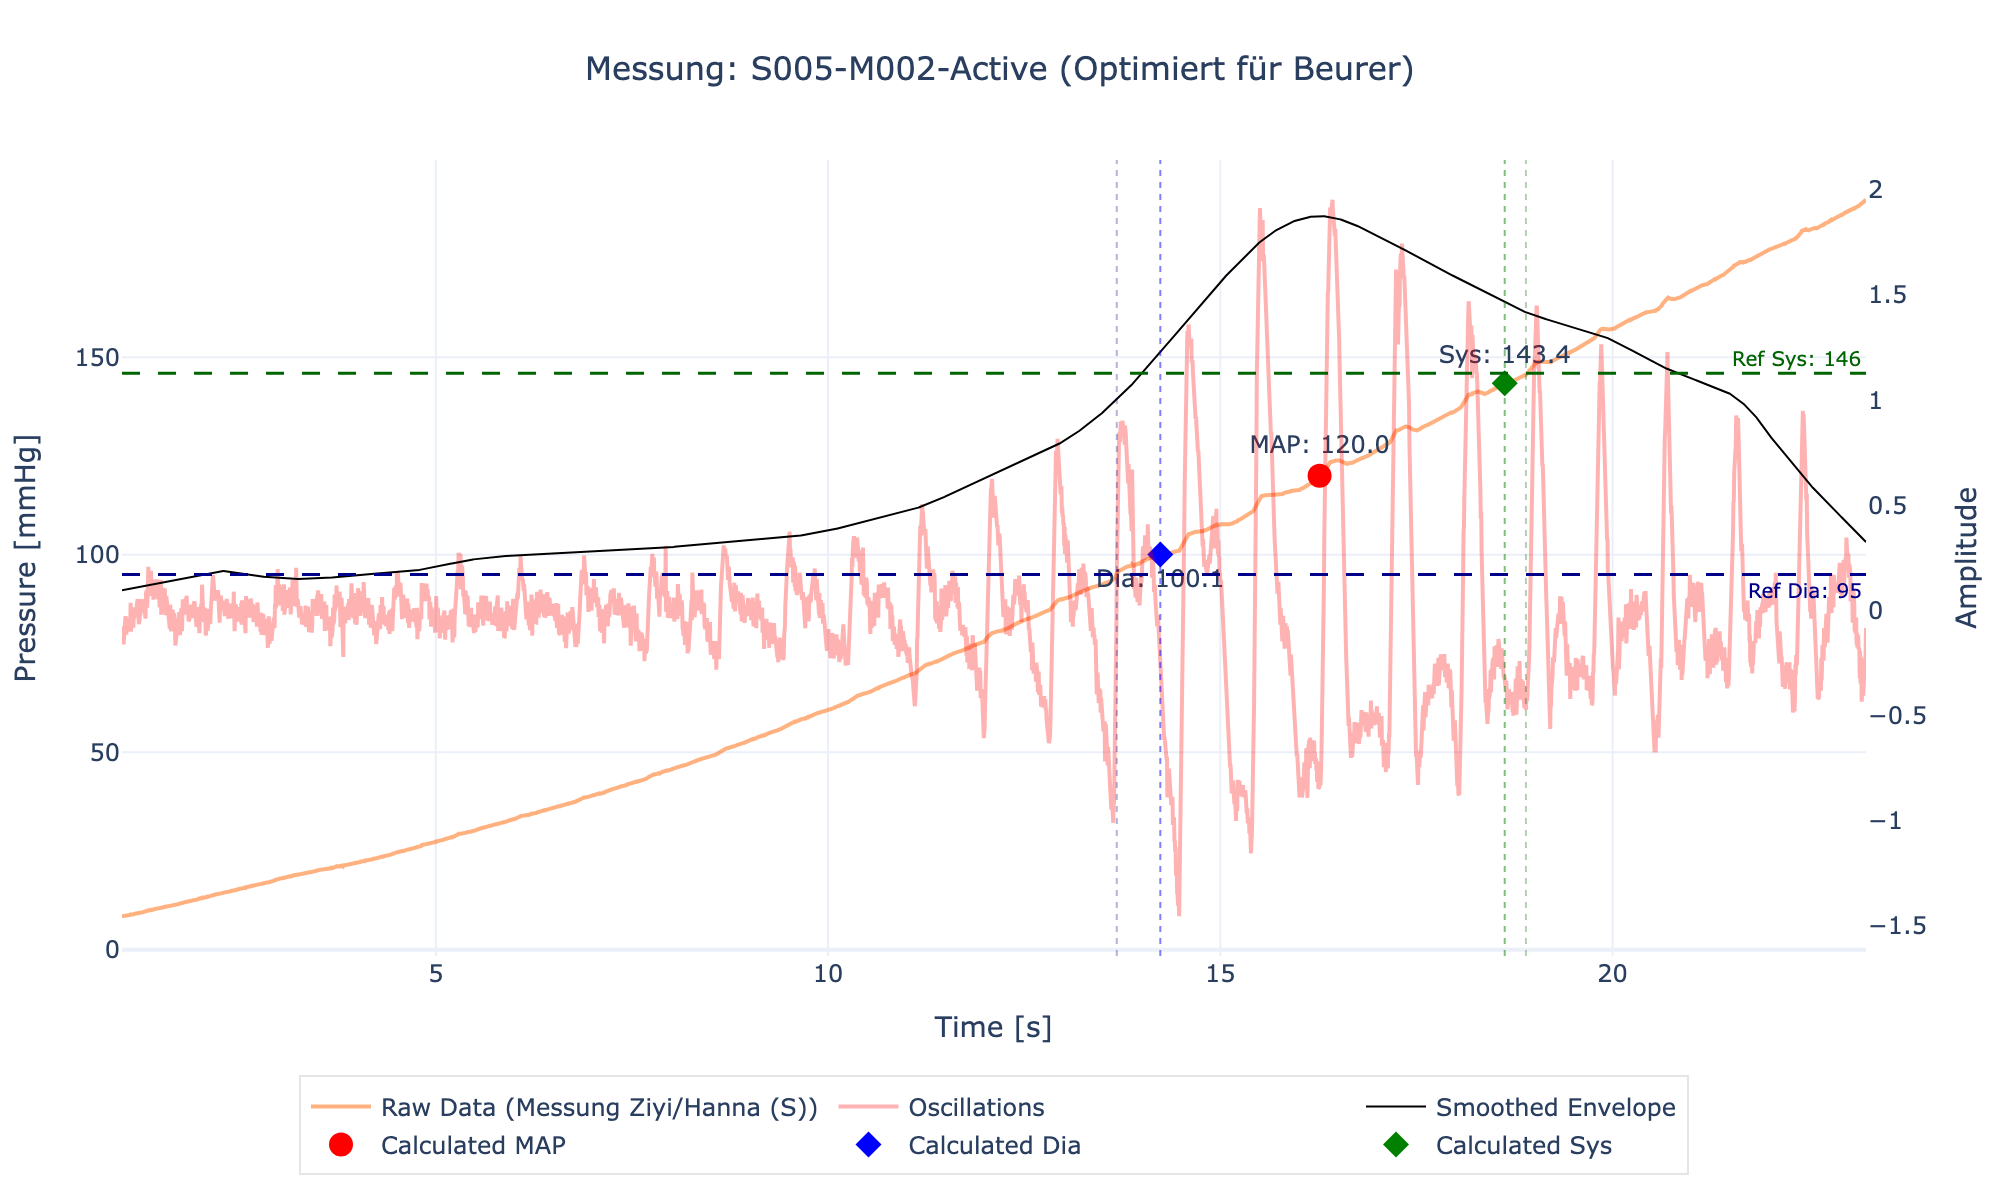
\includegraphics[width=\textwidth]{images/S005-M002-Active_beurer.png}
        \caption{Optimiert für Beurer}
    \end{subfigure}
    \hfill
    \begin{subfigure}[b]{0.48\textwidth}
        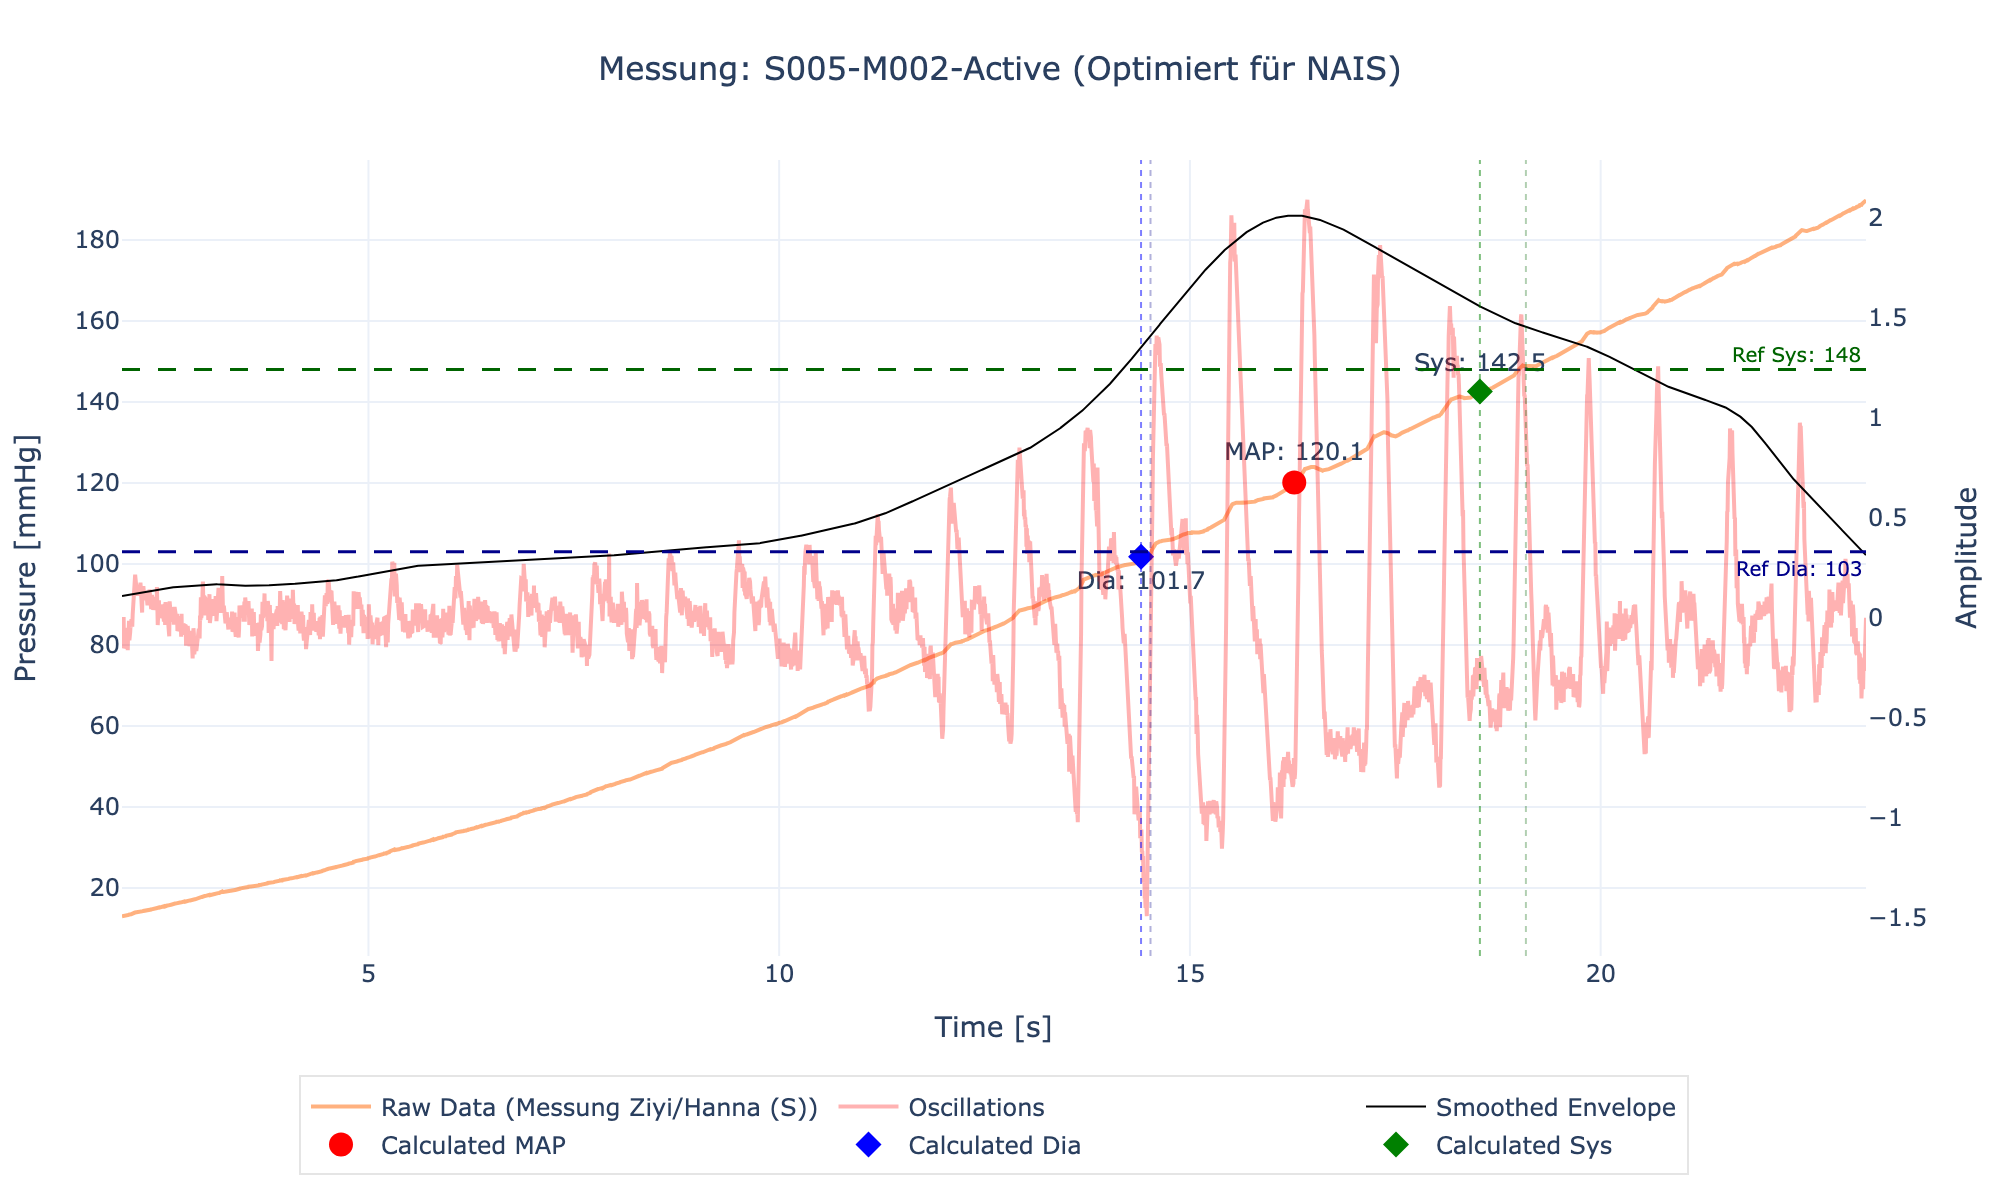
\includegraphics[width=\textwidth]{images/S005-M002-Active_nais.png}
        \caption{Optimiert für NAIS}
    \end{subfigure}
    \caption{Einzelauswertung der Messung S005-M002-Active mit verschiedenen Parametersätzen.}
\end{figure}
\newpage

\subsection*{Messung: S006-M001-Rest}
\begin{figure}[H]
    \centering
    \begin{subfigure}[b]{0.8\textwidth}
        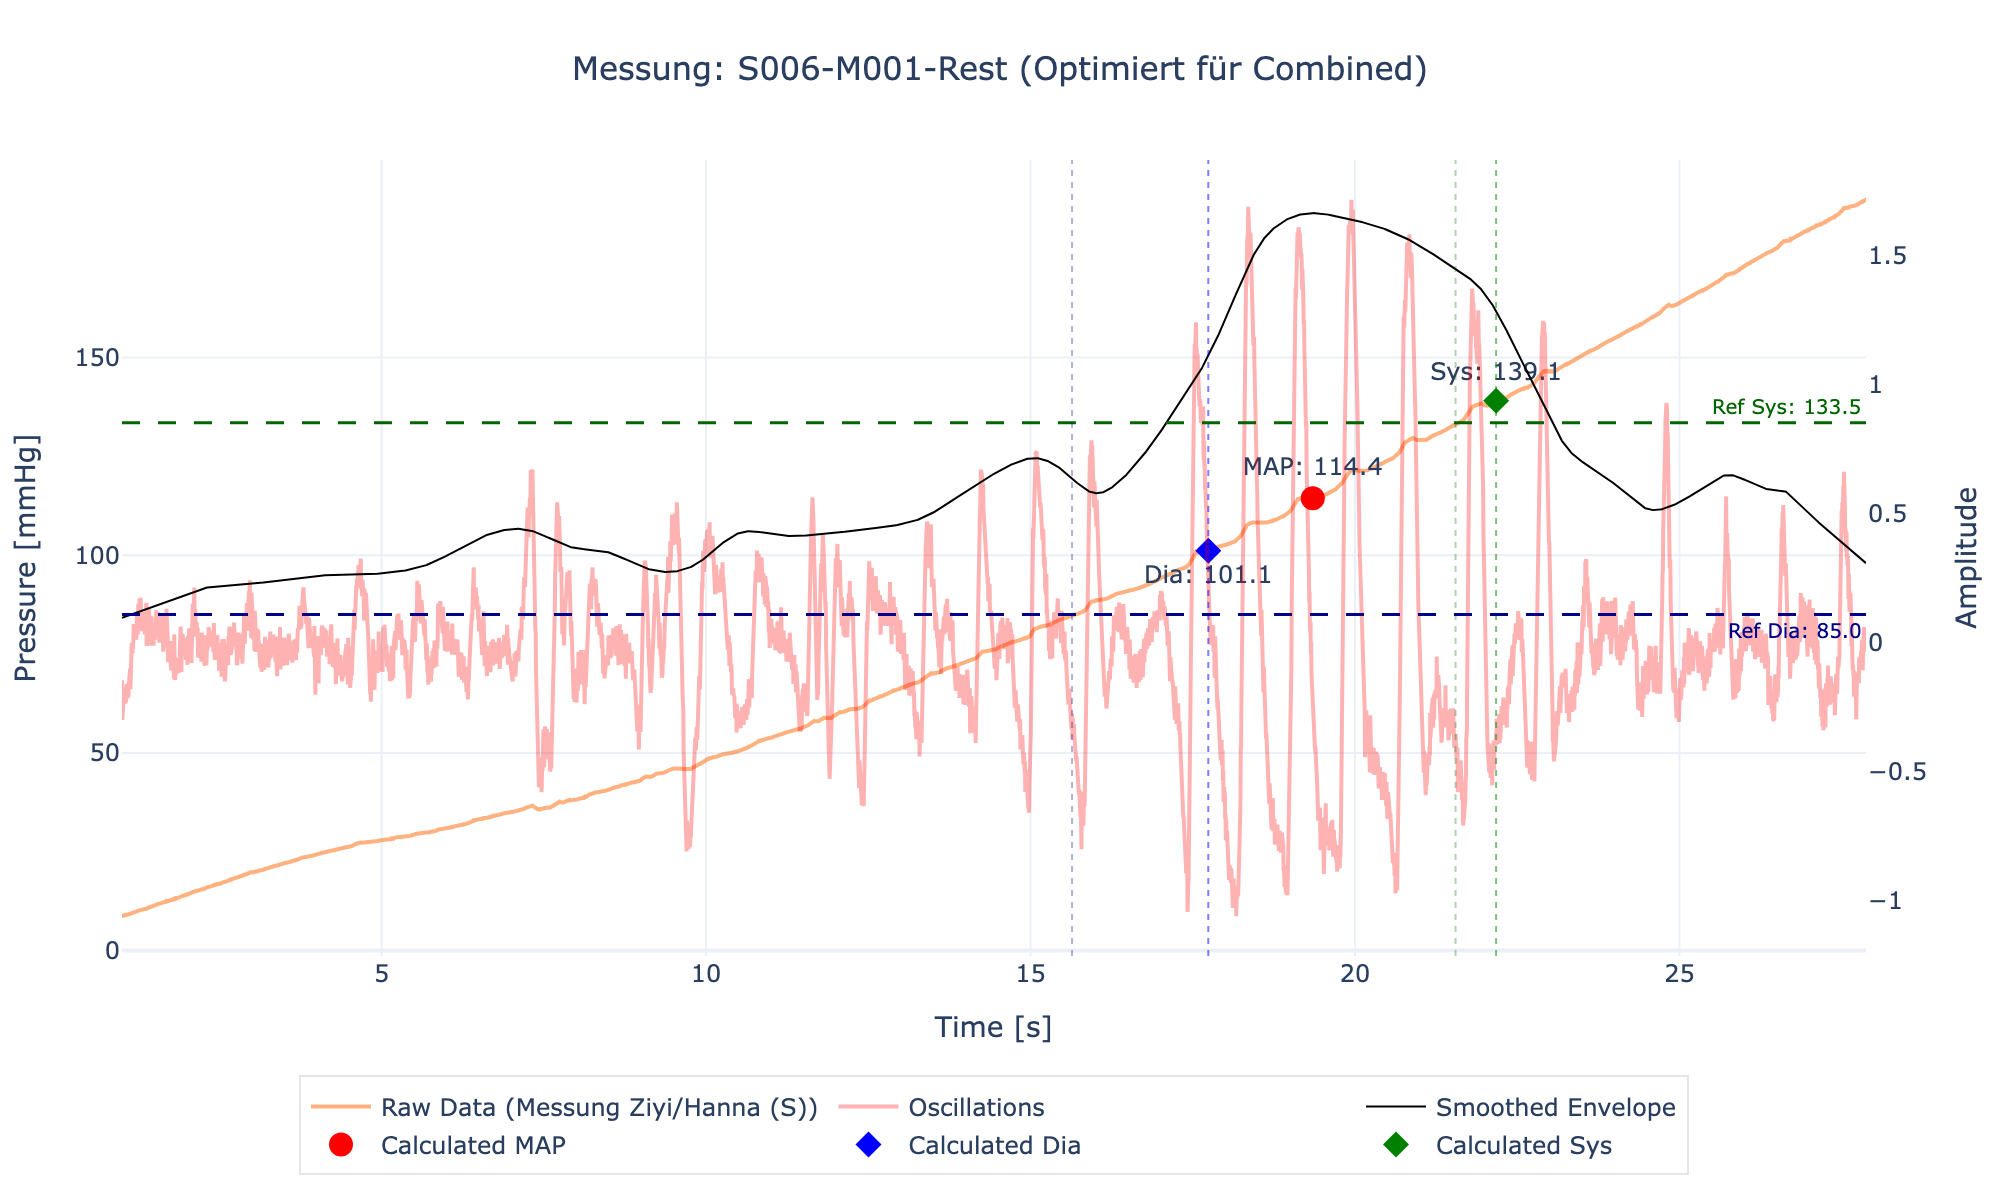
\includegraphics[width=\textwidth]{images/S006-M001-Rest_combined.png}
        \caption{Optimiert für Beurer und NAIS (Kombiniert)}
    \end{subfigure} \\
    \begin{subfigure}[b]{0.48\textwidth}
        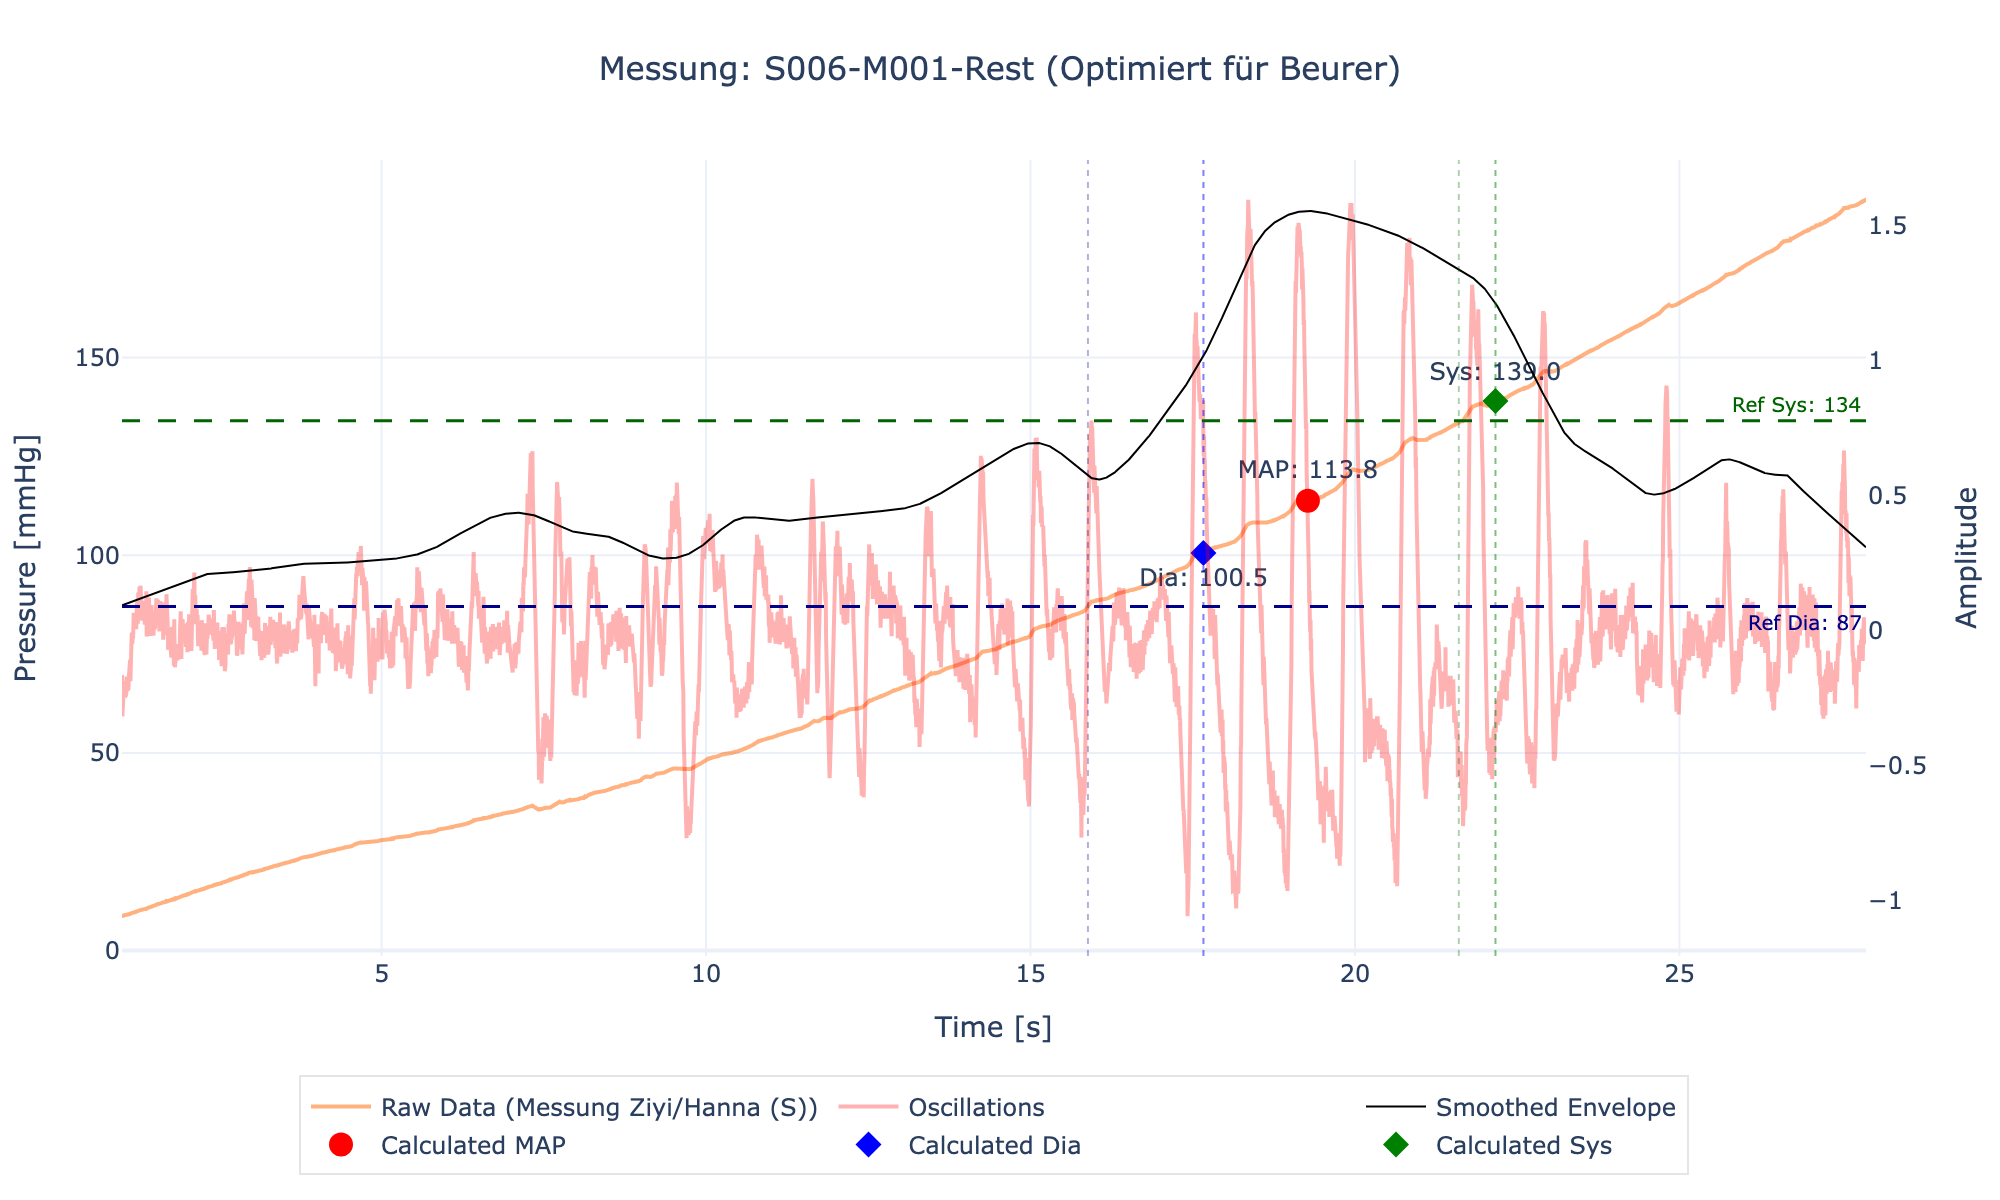
\includegraphics[width=\textwidth]{images/S006-M001-Rest_beurer.png}
        \caption{Optimiert für Beurer}
    \end{subfigure}
    \hfill
    \begin{subfigure}[b]{0.48\textwidth}
        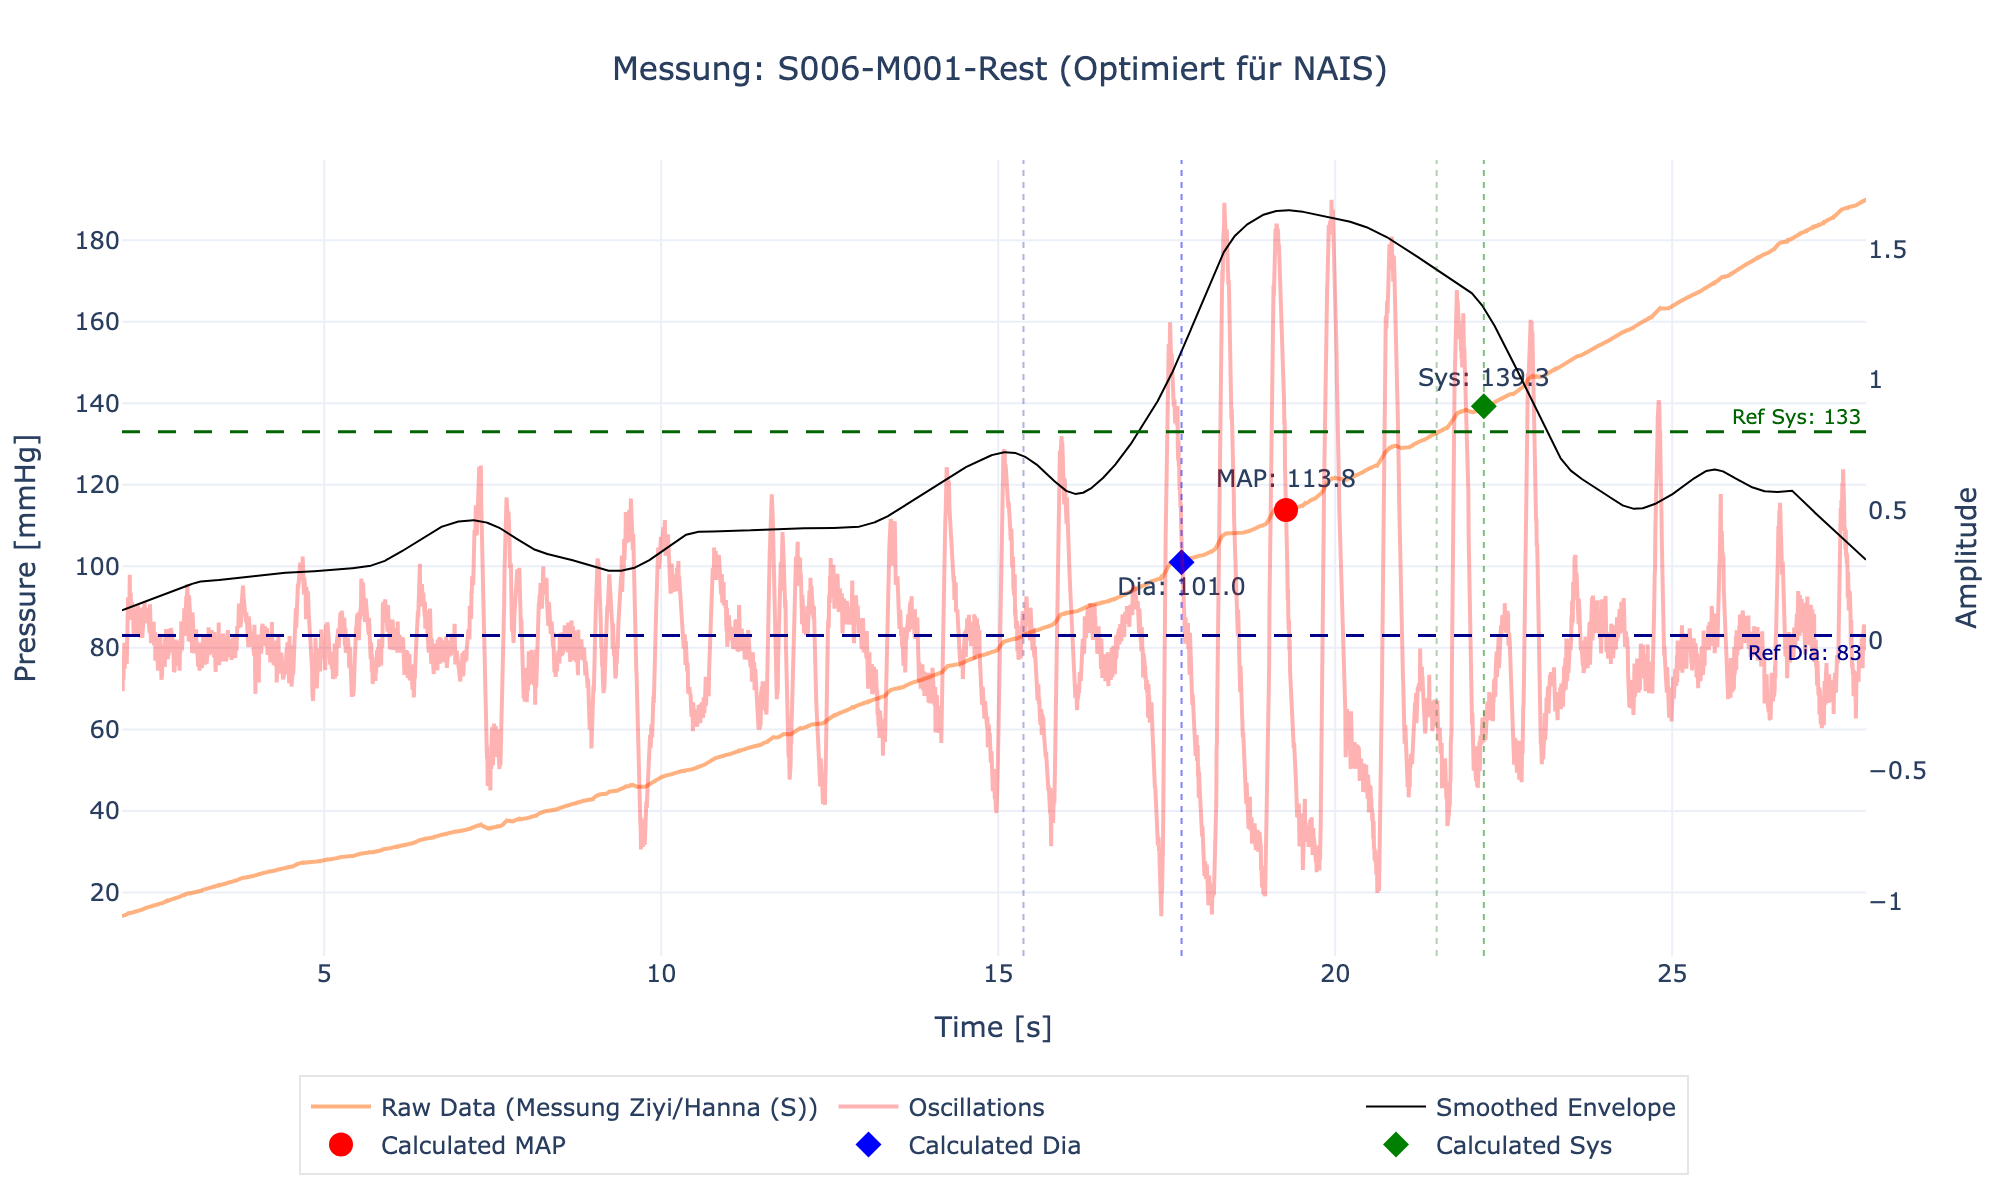
\includegraphics[width=\textwidth]{images/S006-M001-Rest_nais.png}
        \caption{Optimiert für NAIS}
    \end{subfigure}
    \caption{Einzelauswertung der Messung S006-M001-Rest mit verschiedenen Parametersätzen.}
\end{figure}
\newpage

\subsection*{Messung: S006-M002-Active}
\begin{figure}[H]
    \centering
    \begin{subfigure}[b]{0.8\textwidth}
        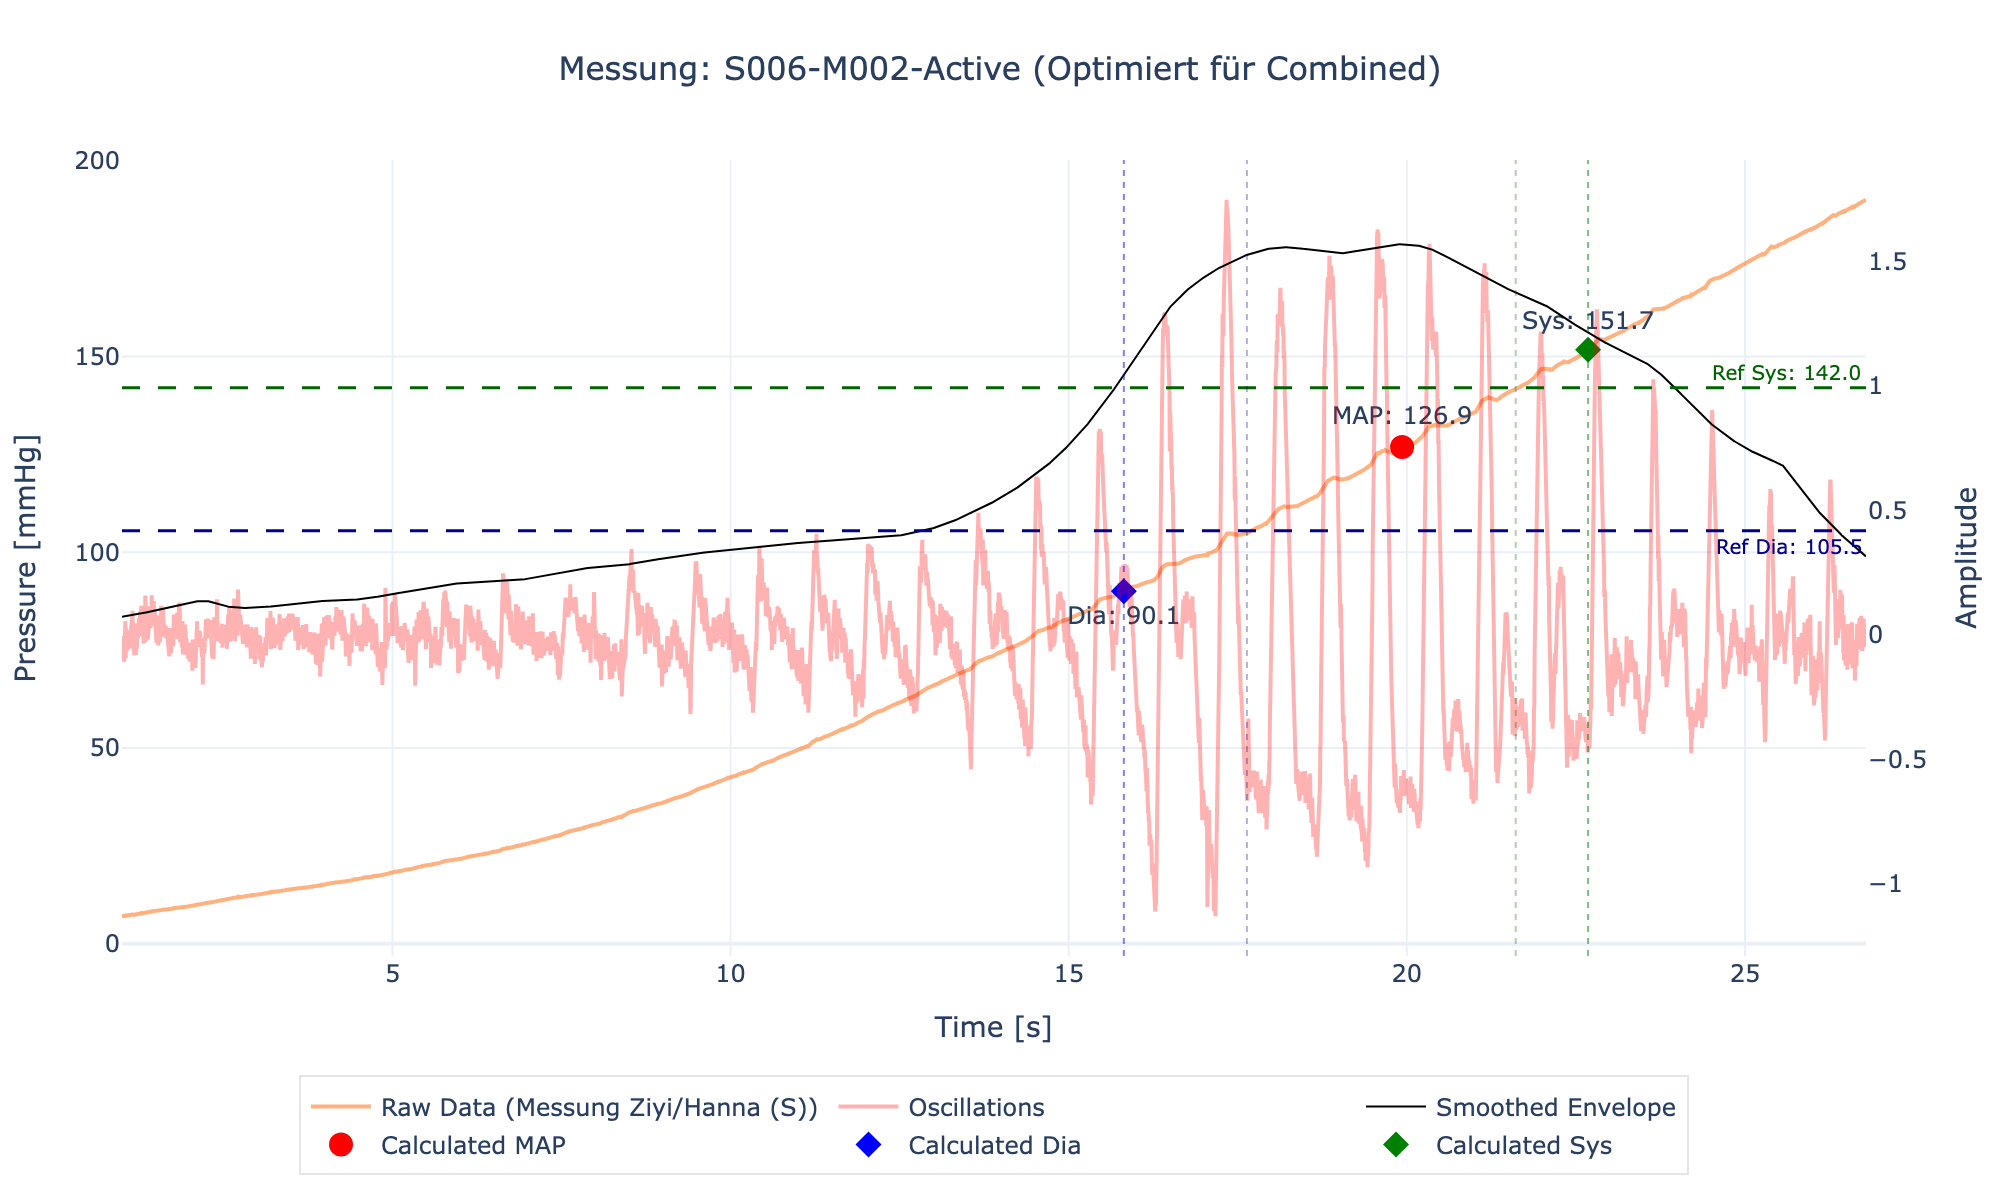
\includegraphics[width=\textwidth]{images/S006-M002-Active_combined.png}
        \caption{Optimiert für Beurer und NAIS (Kombiniert)}
    \end{subfigure} \\
    \begin{subfigure}[b]{0.48\textwidth}
        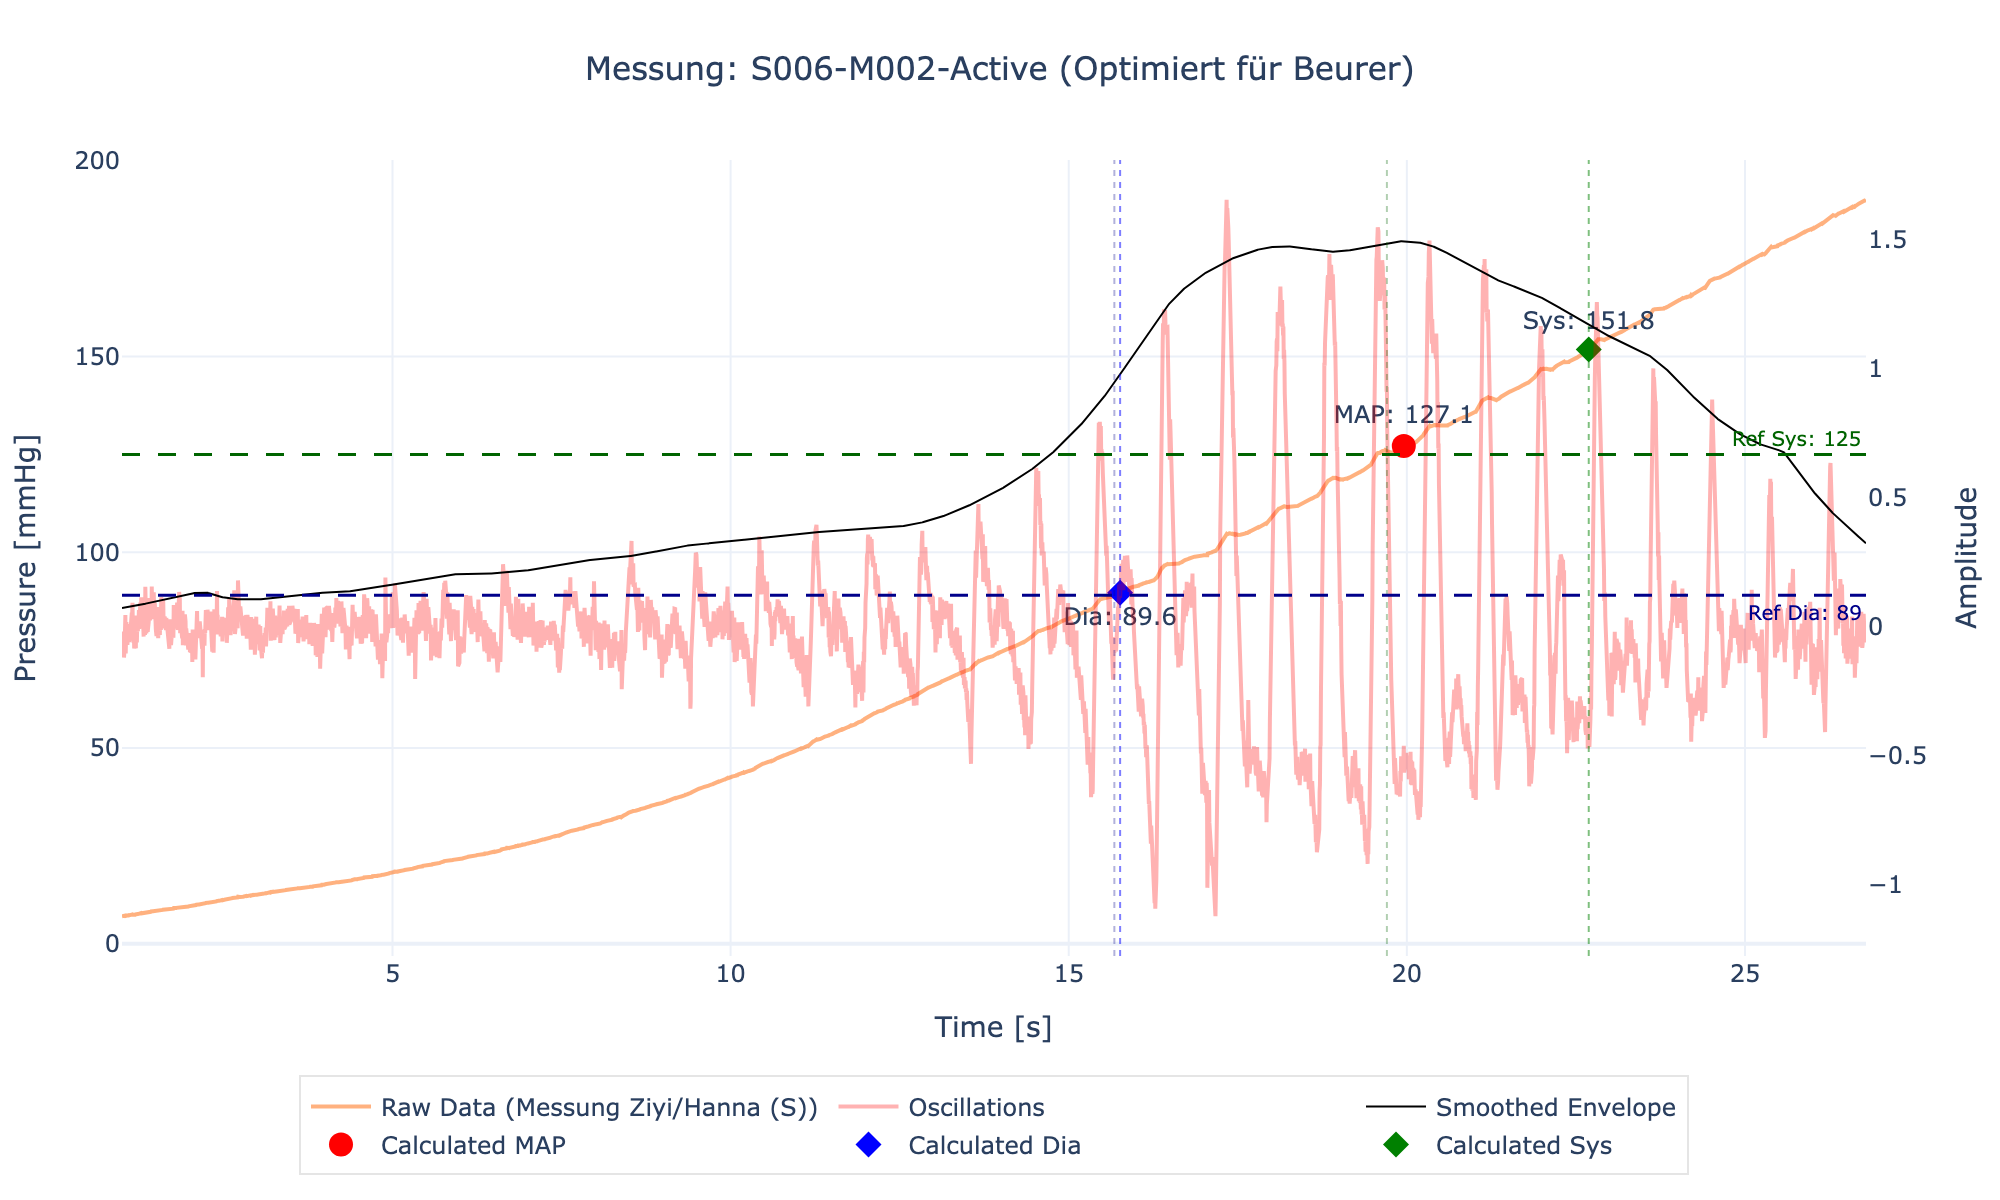
\includegraphics[width=\textwidth]{images/S006-M002-Active_beurer.png}
        \caption{Optimiert für Beurer}
    \end{subfigure}
    \hfill
    \begin{subfigure}[b]{0.48\textwidth}
        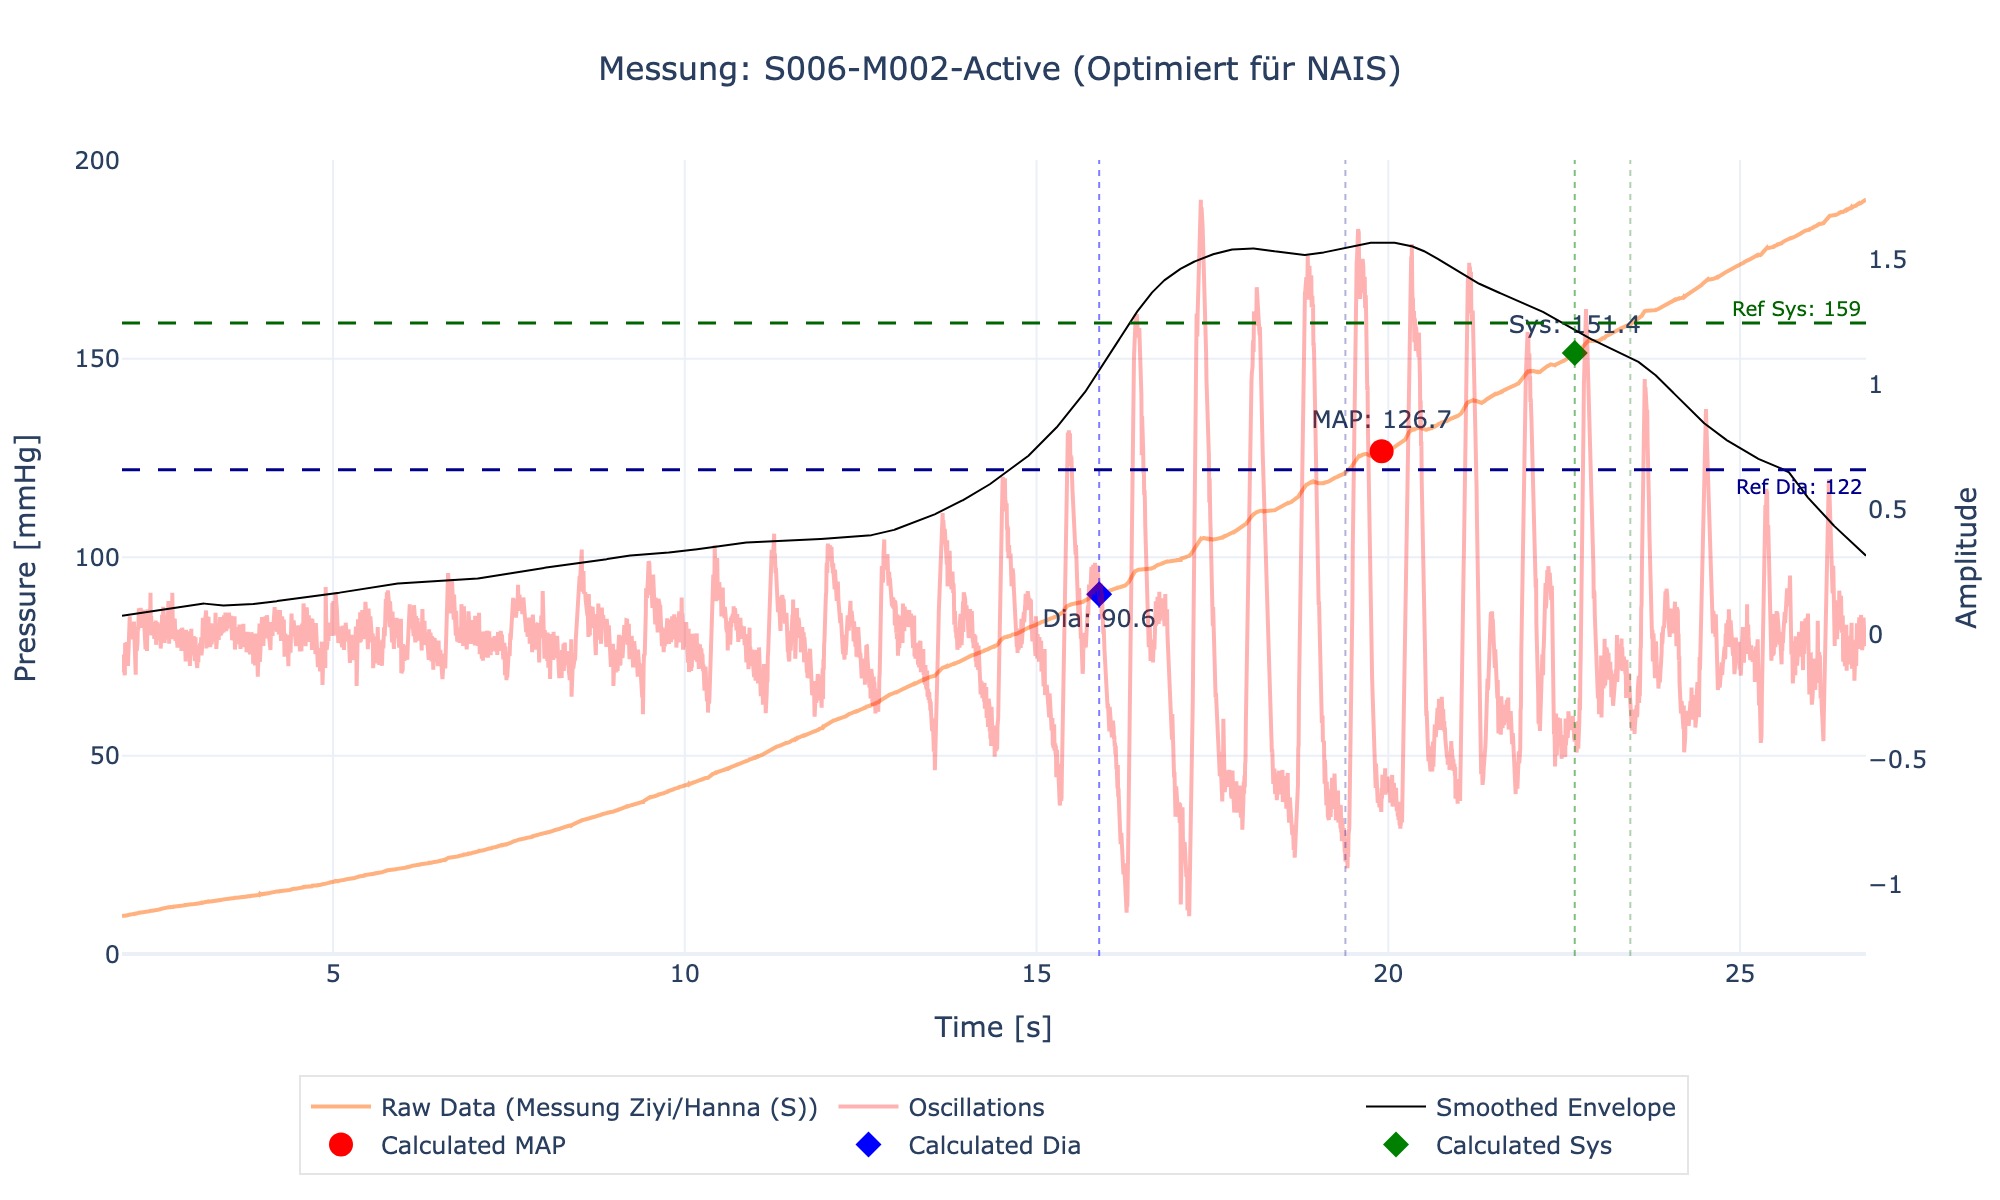
\includegraphics[width=\textwidth]{images/S006-M002-Active_nais.png}
        \caption{Optimiert für NAIS}
    \end{subfigure}
    \caption{Einzelauswertung der Messung S006-M002-Active mit verschiedenen Parametersätzen.}
\end{figure}
\newpage

\subsection*{Messung: S007-M001-Rest}
\begin{figure}[H]
    \centering
    \begin{subfigure}[b]{0.8\textwidth}
        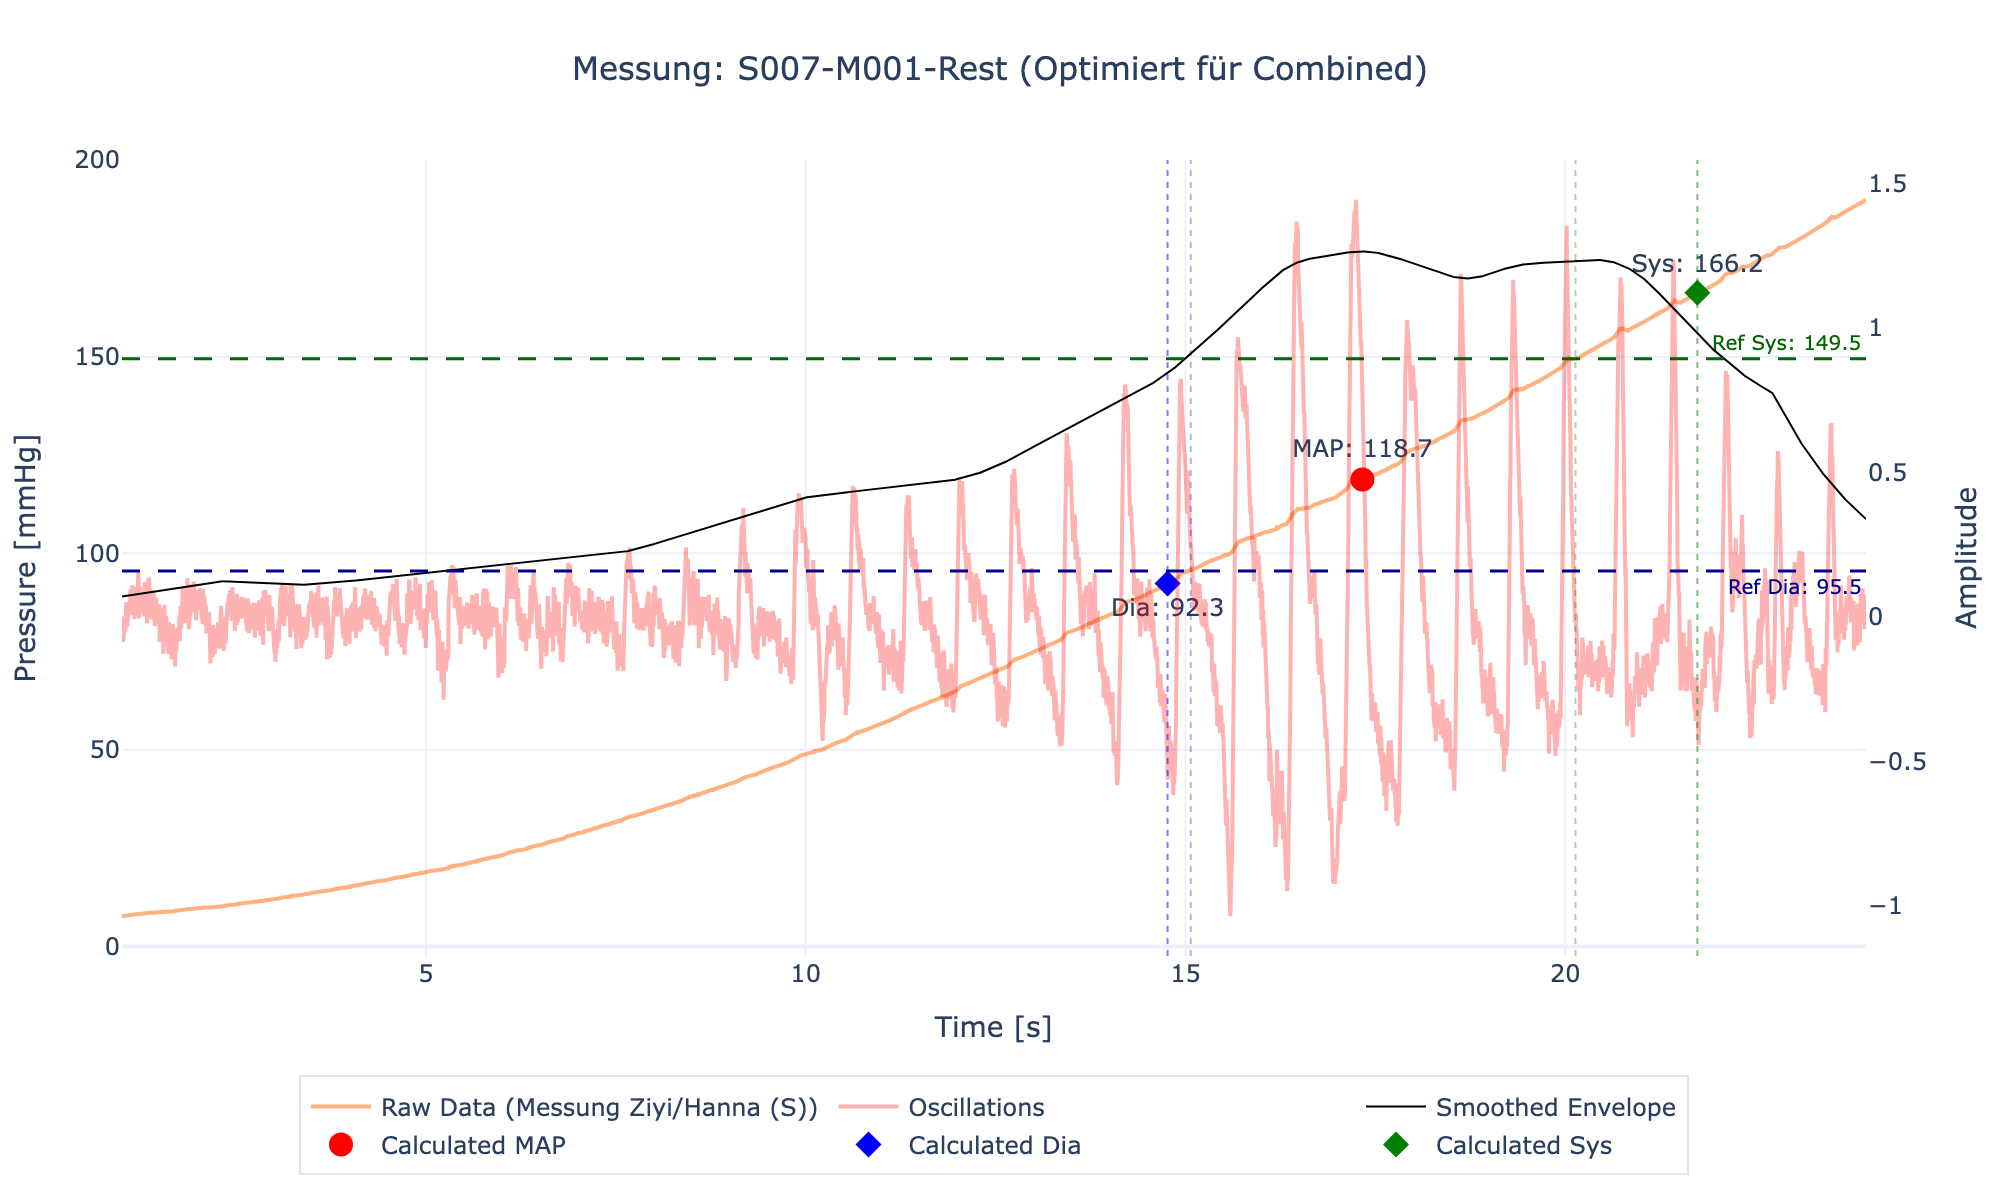
\includegraphics[width=\textwidth]{images/S007-M001-Rest_combined.png}
        \caption{Optimiert für Beurer und NAIS (Kombiniert)}
    \end{subfigure} \\
    \begin{subfigure}[b]{0.48\textwidth}
        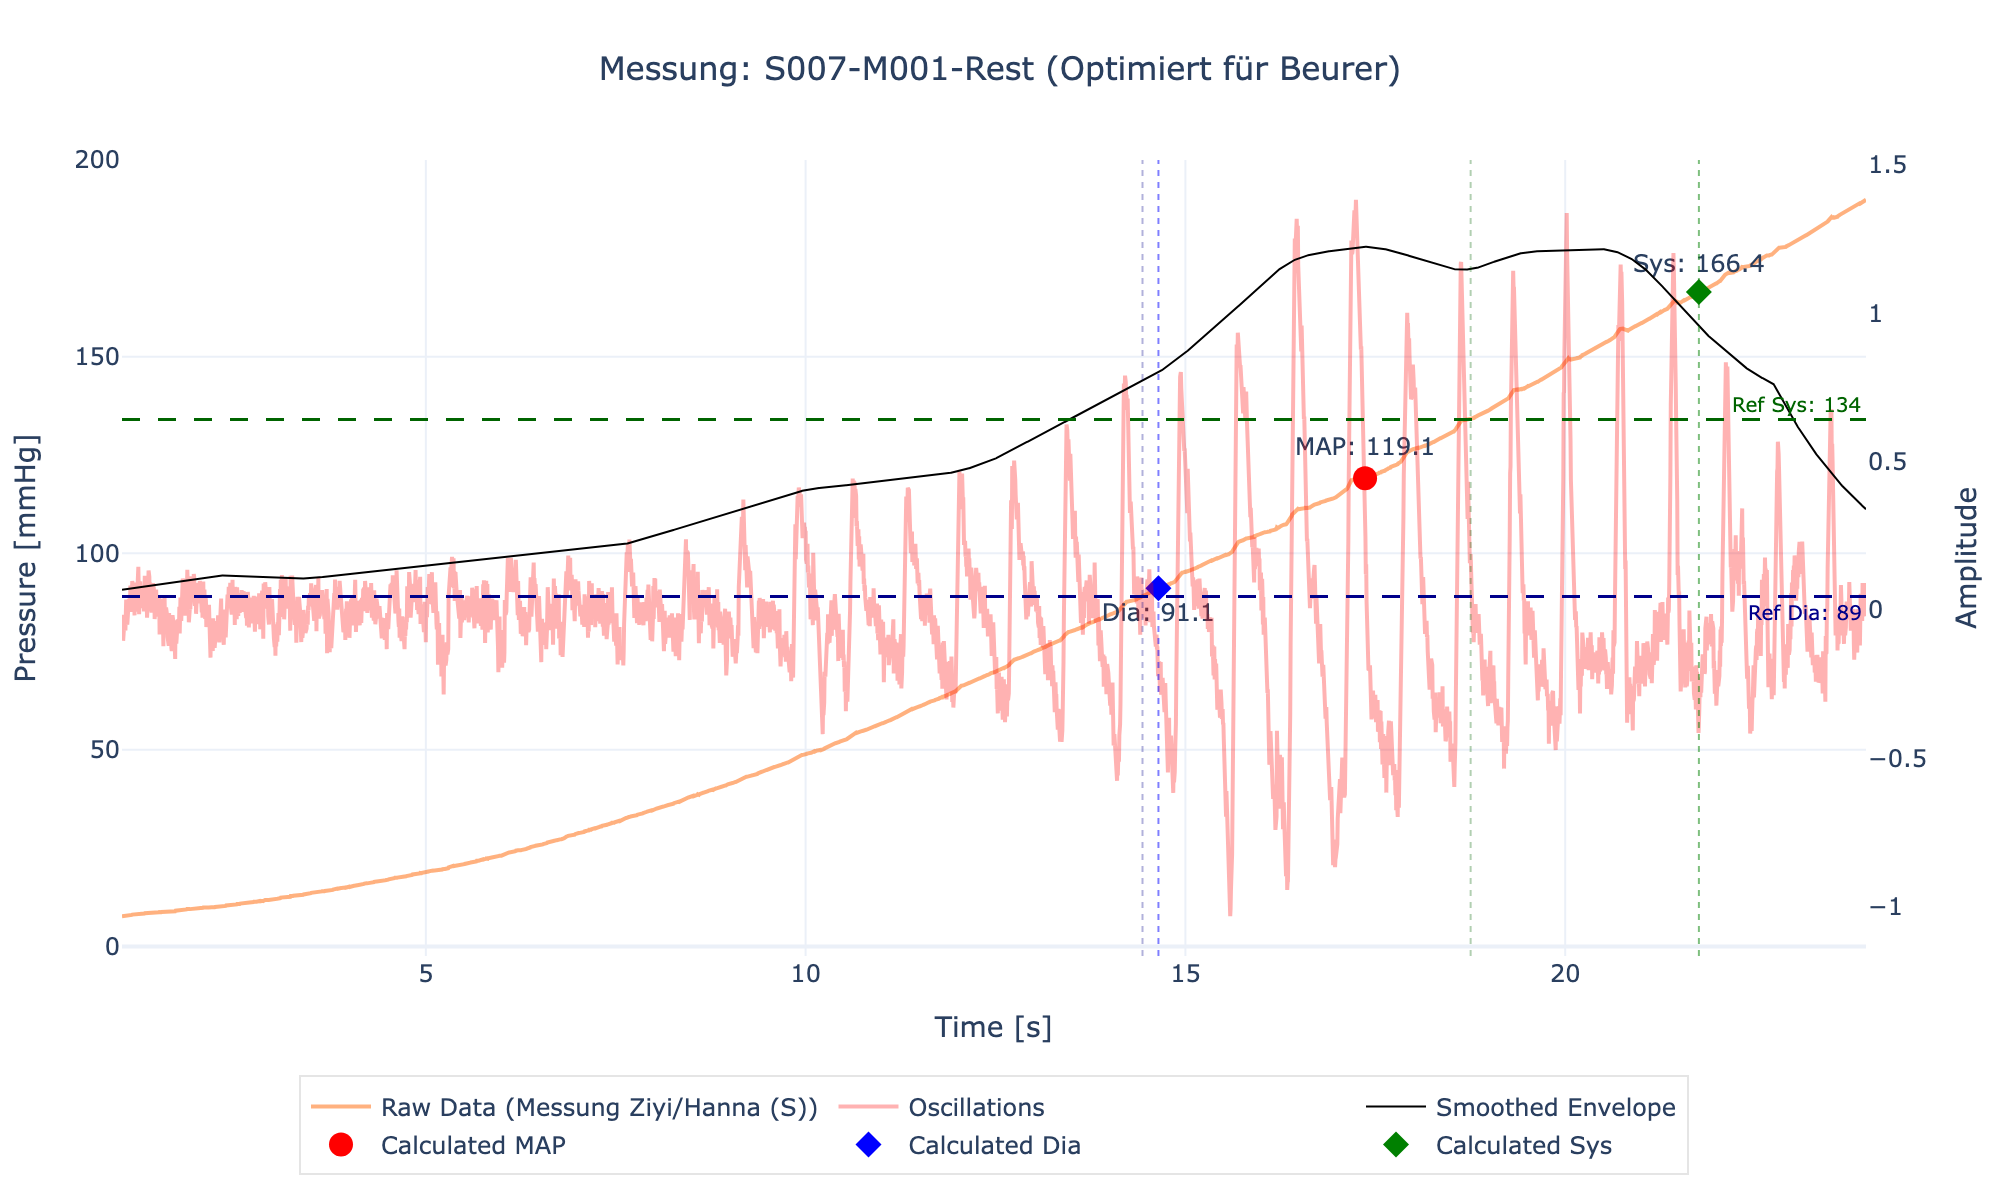
\includegraphics[width=\textwidth]{images/S007-M001-Rest_beurer.png}
        \caption{Optimiert für Beurer}
    \end{subfigure}
    \hfill
    \begin{subfigure}[b]{0.48\textwidth}
        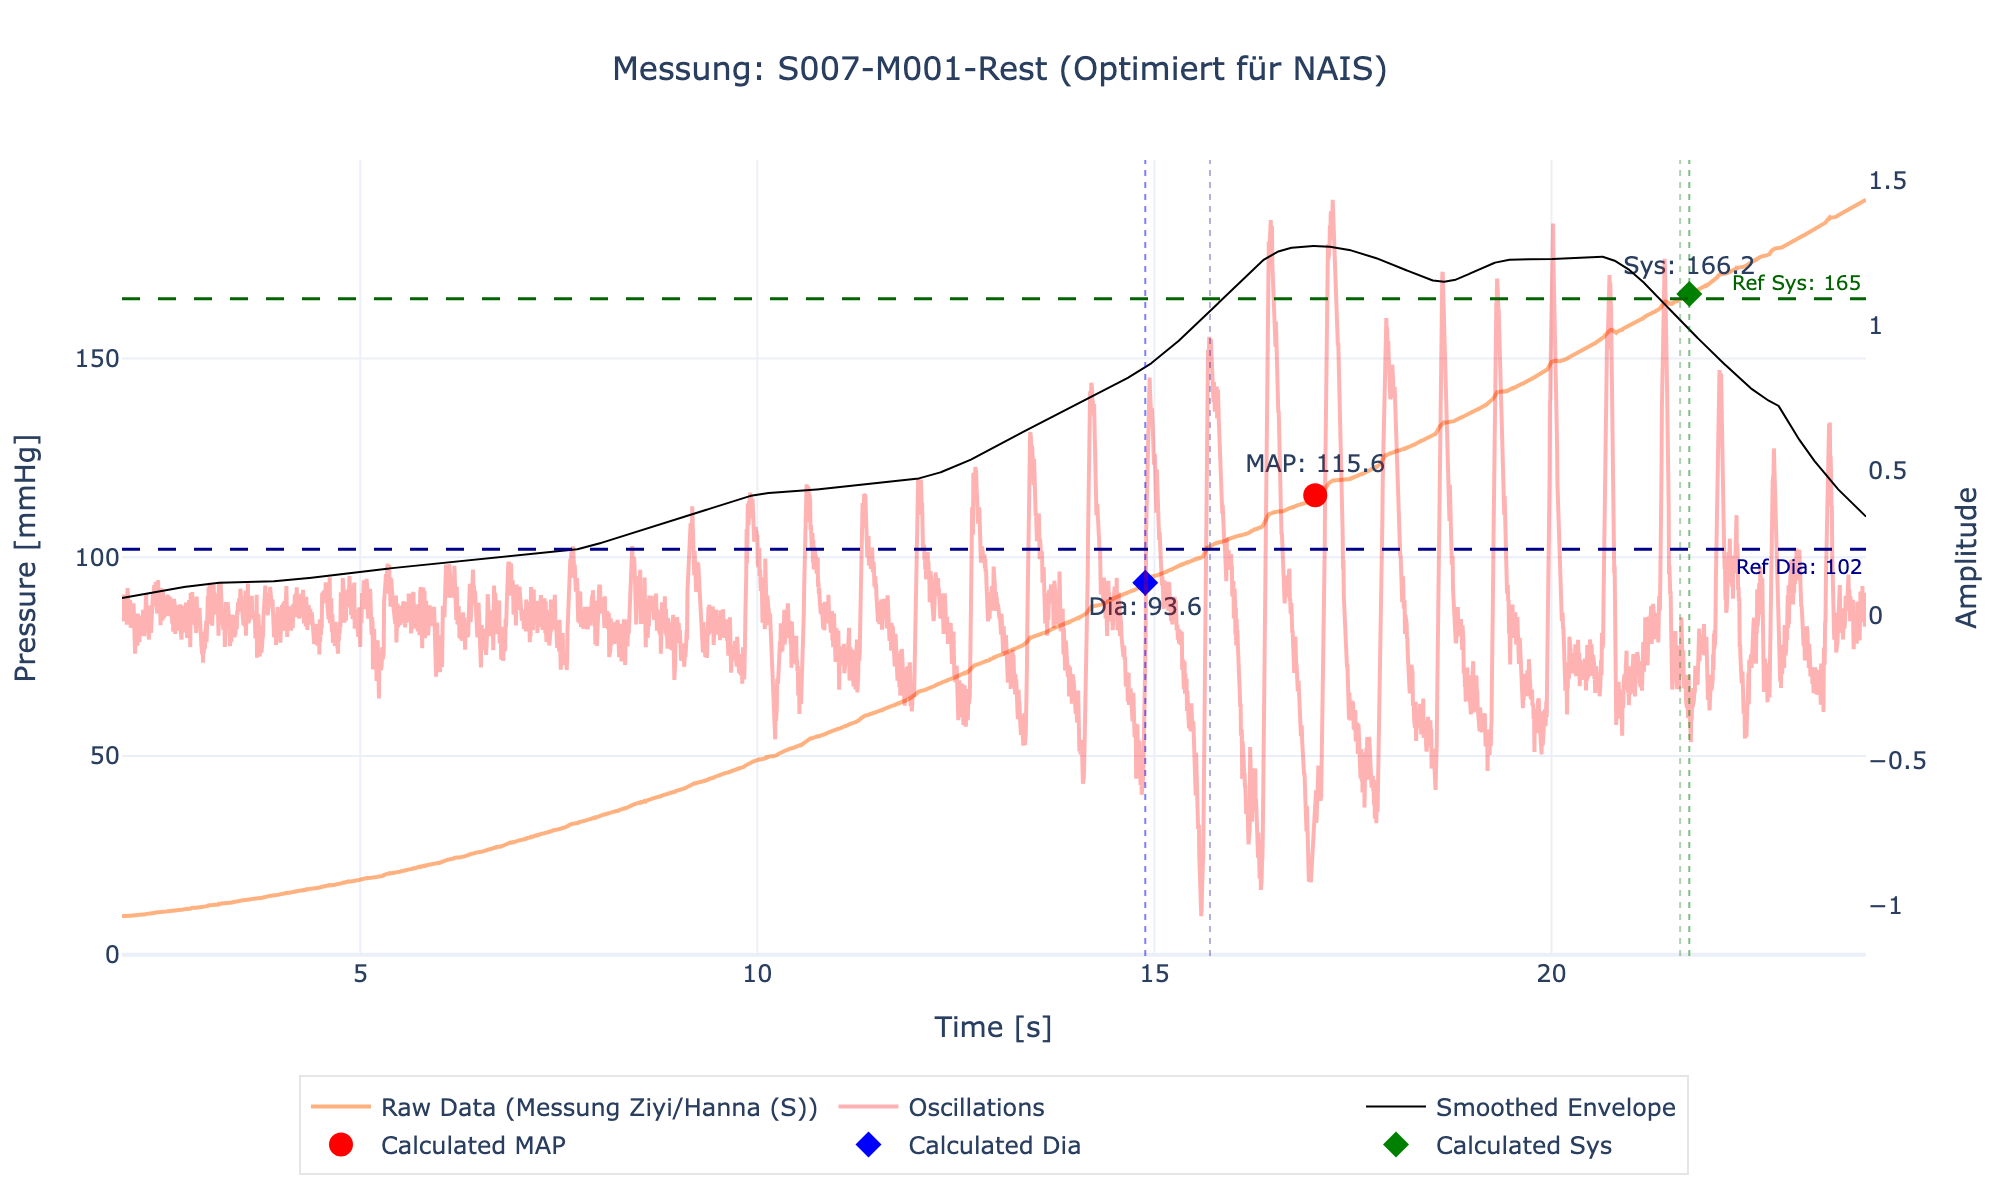
\includegraphics[width=\textwidth]{images/S007-M001-Rest_nais.png}
        \caption{Optimiert für NAIS}
    \end{subfigure}
    \caption{Einzelauswertung der Messung S007-M001-Rest mit verschiedenen Parametersätzen.}
\end{figure}
\newpage

\subsection*{Messung: S007-M002-Active}
\begin{figure}[H]
    \centering
    \begin{subfigure}[b]{0.8\textwidth}
        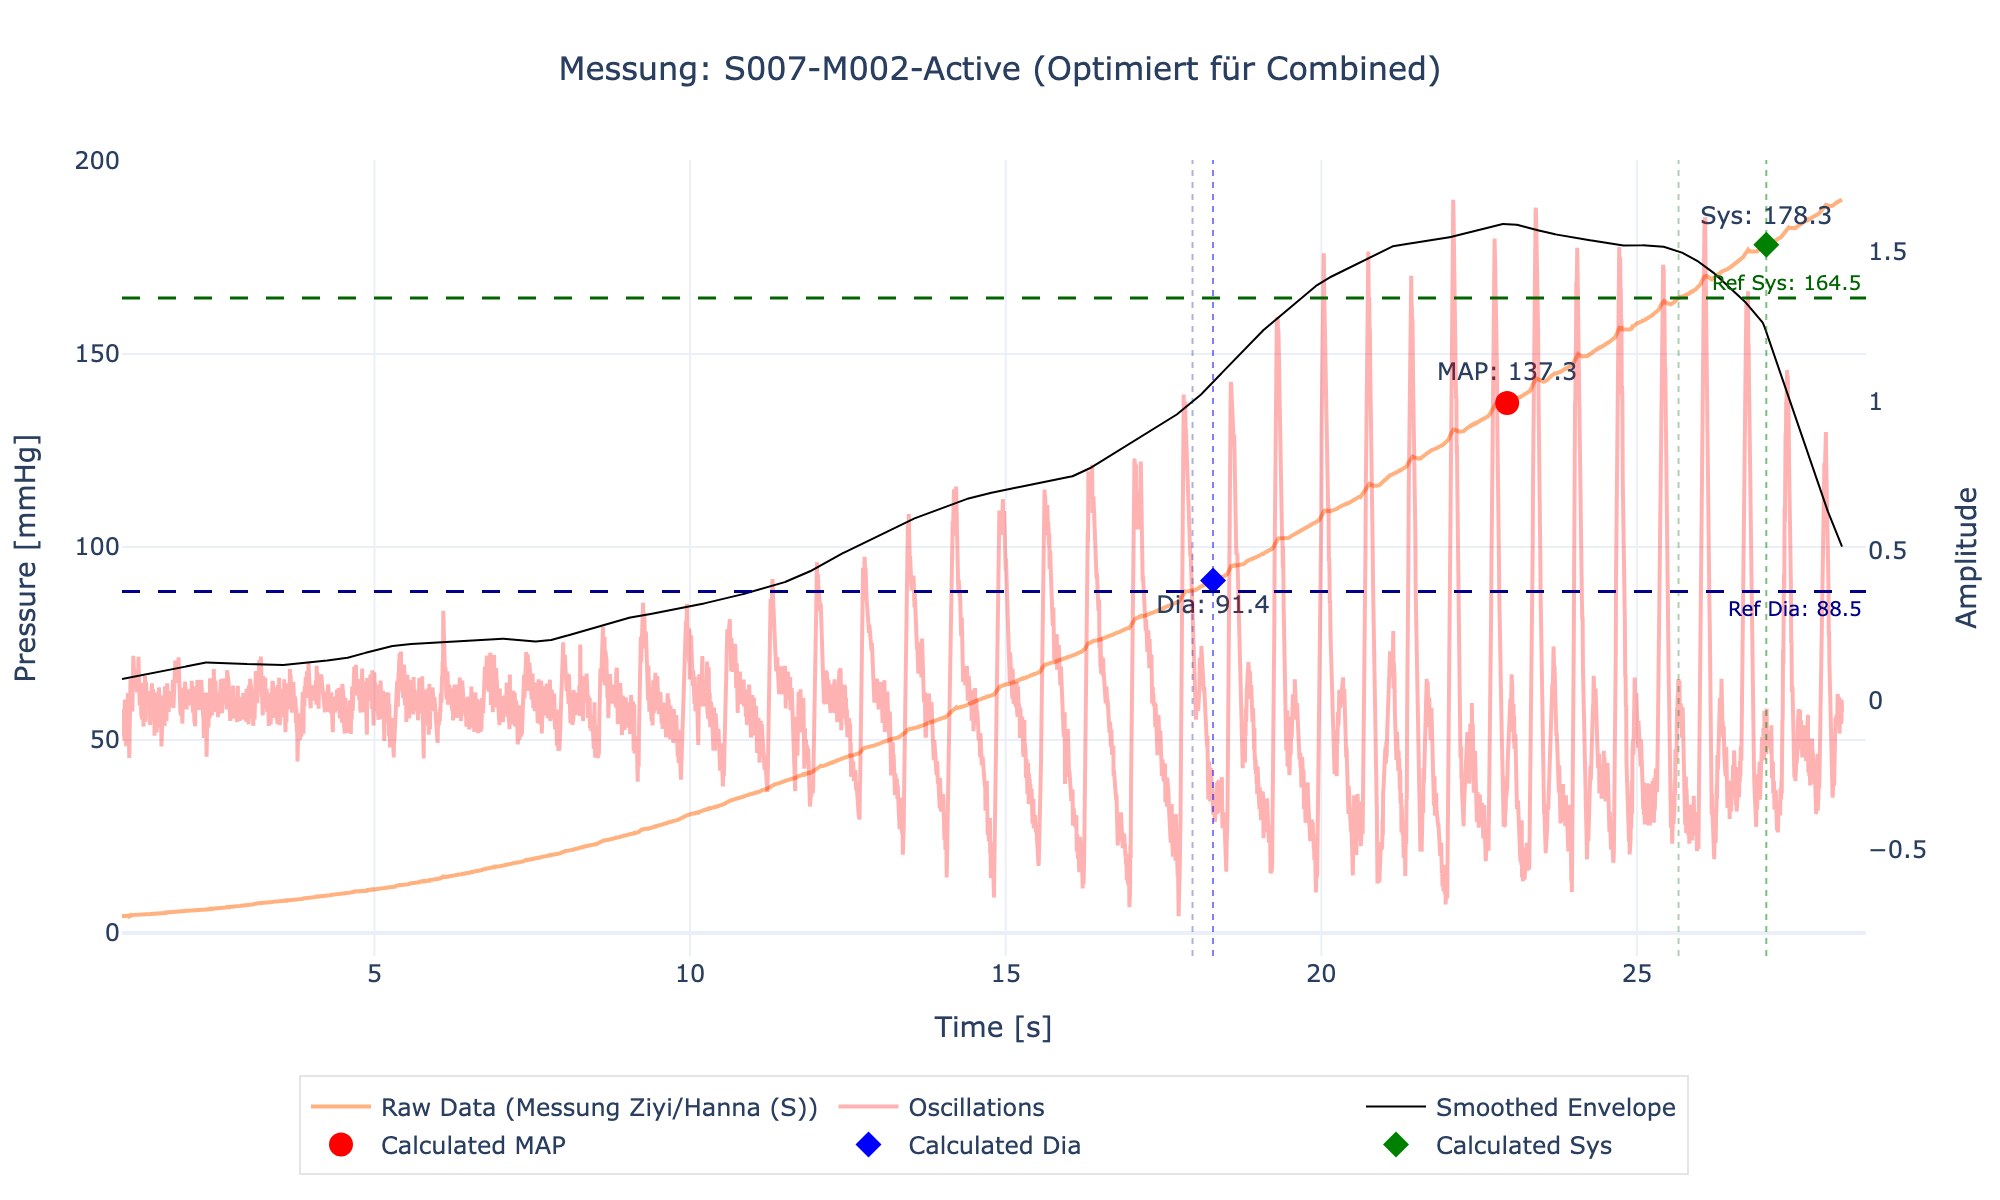
\includegraphics[width=\textwidth]{images/S007-M002-Active_combined.png}
        \caption{Optimiert für Beurer und NAIS (Kombiniert)}
    \end{subfigure} \\
    \begin{subfigure}[b]{0.48\textwidth}
        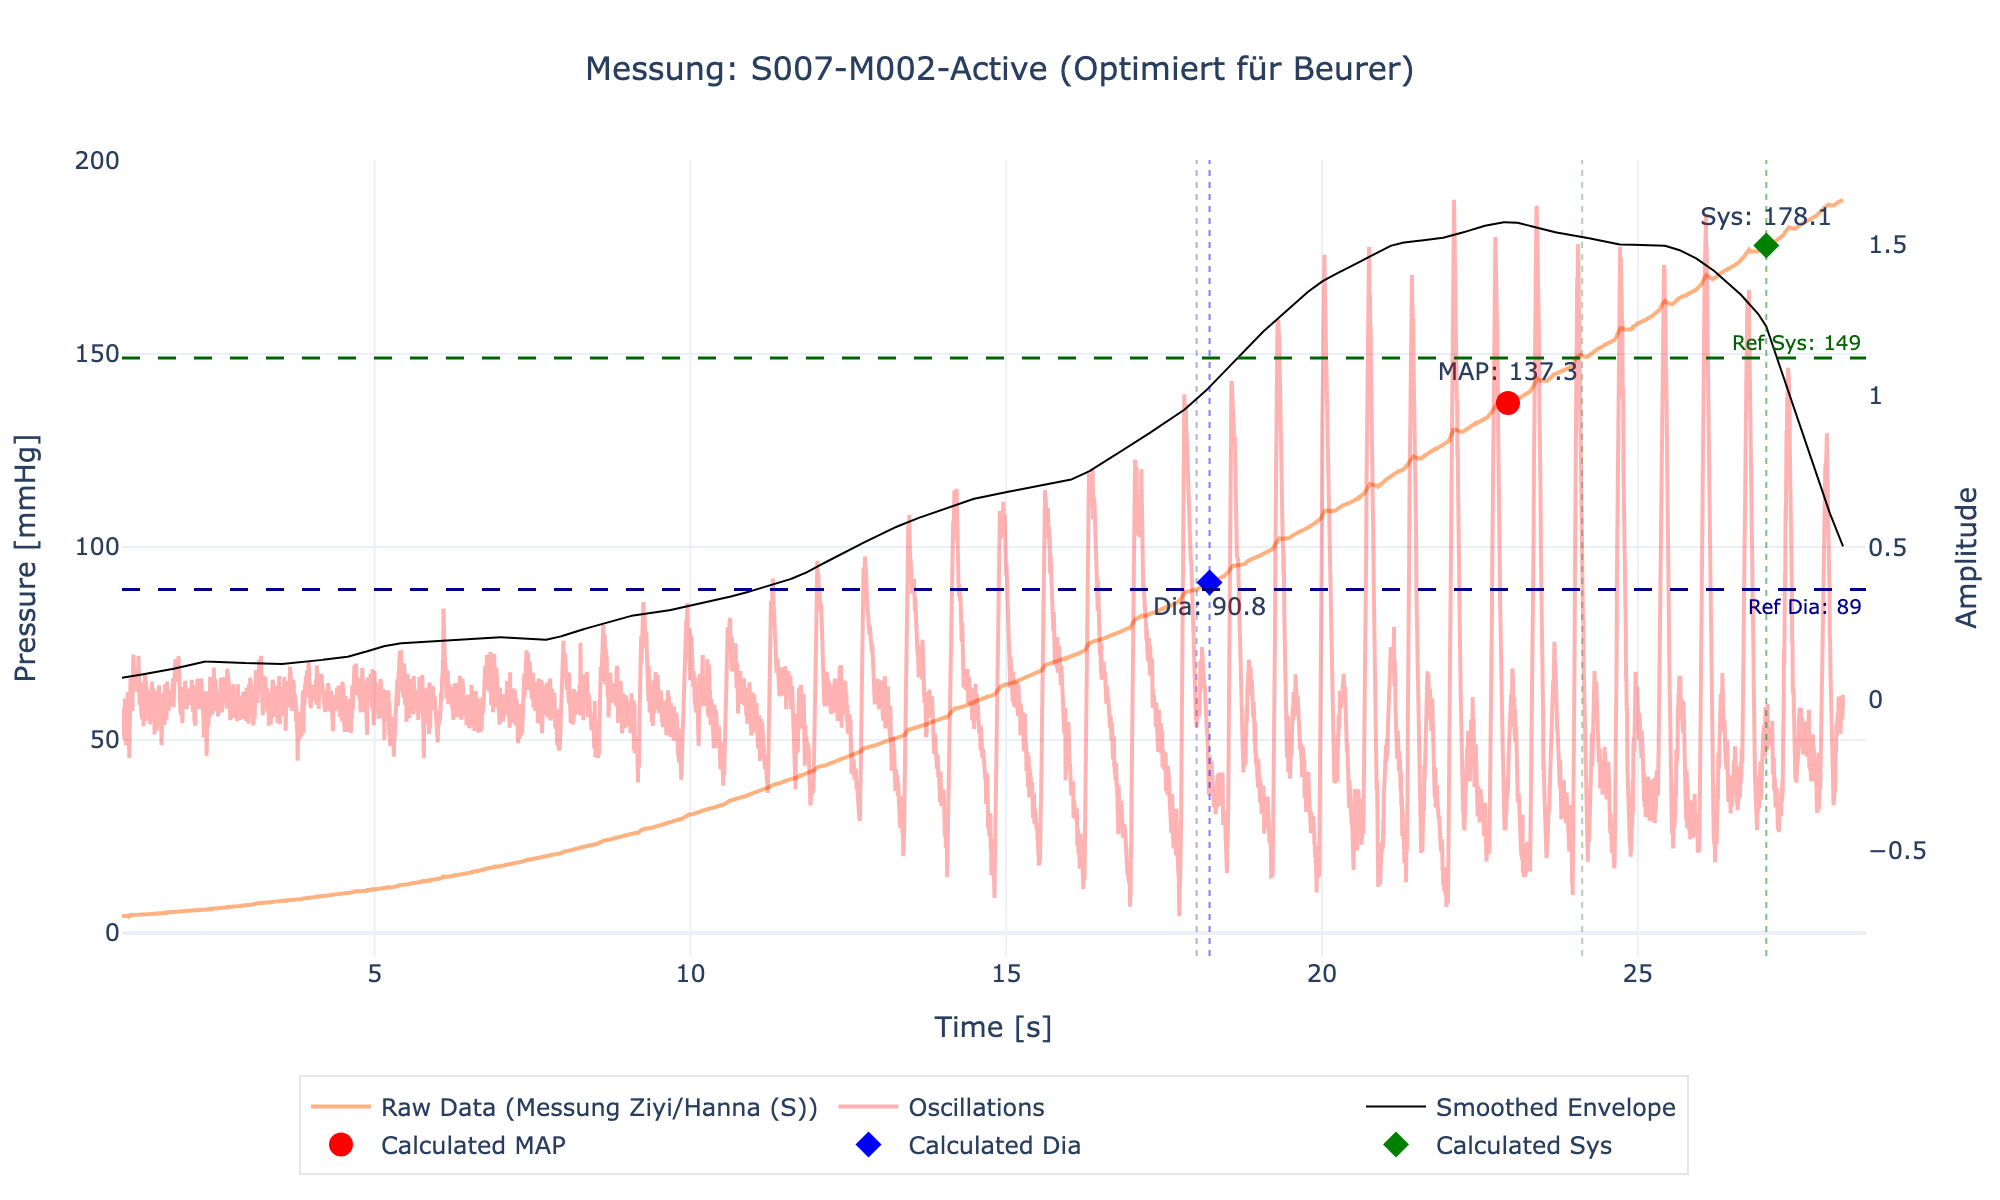
\includegraphics[width=\textwidth]{images/S007-M002-Active_beurer.png}
        \caption{Optimiert für Beurer}
    \end{subfigure}
    \hfill
    \begin{subfigure}[b]{0.48\textwidth}
        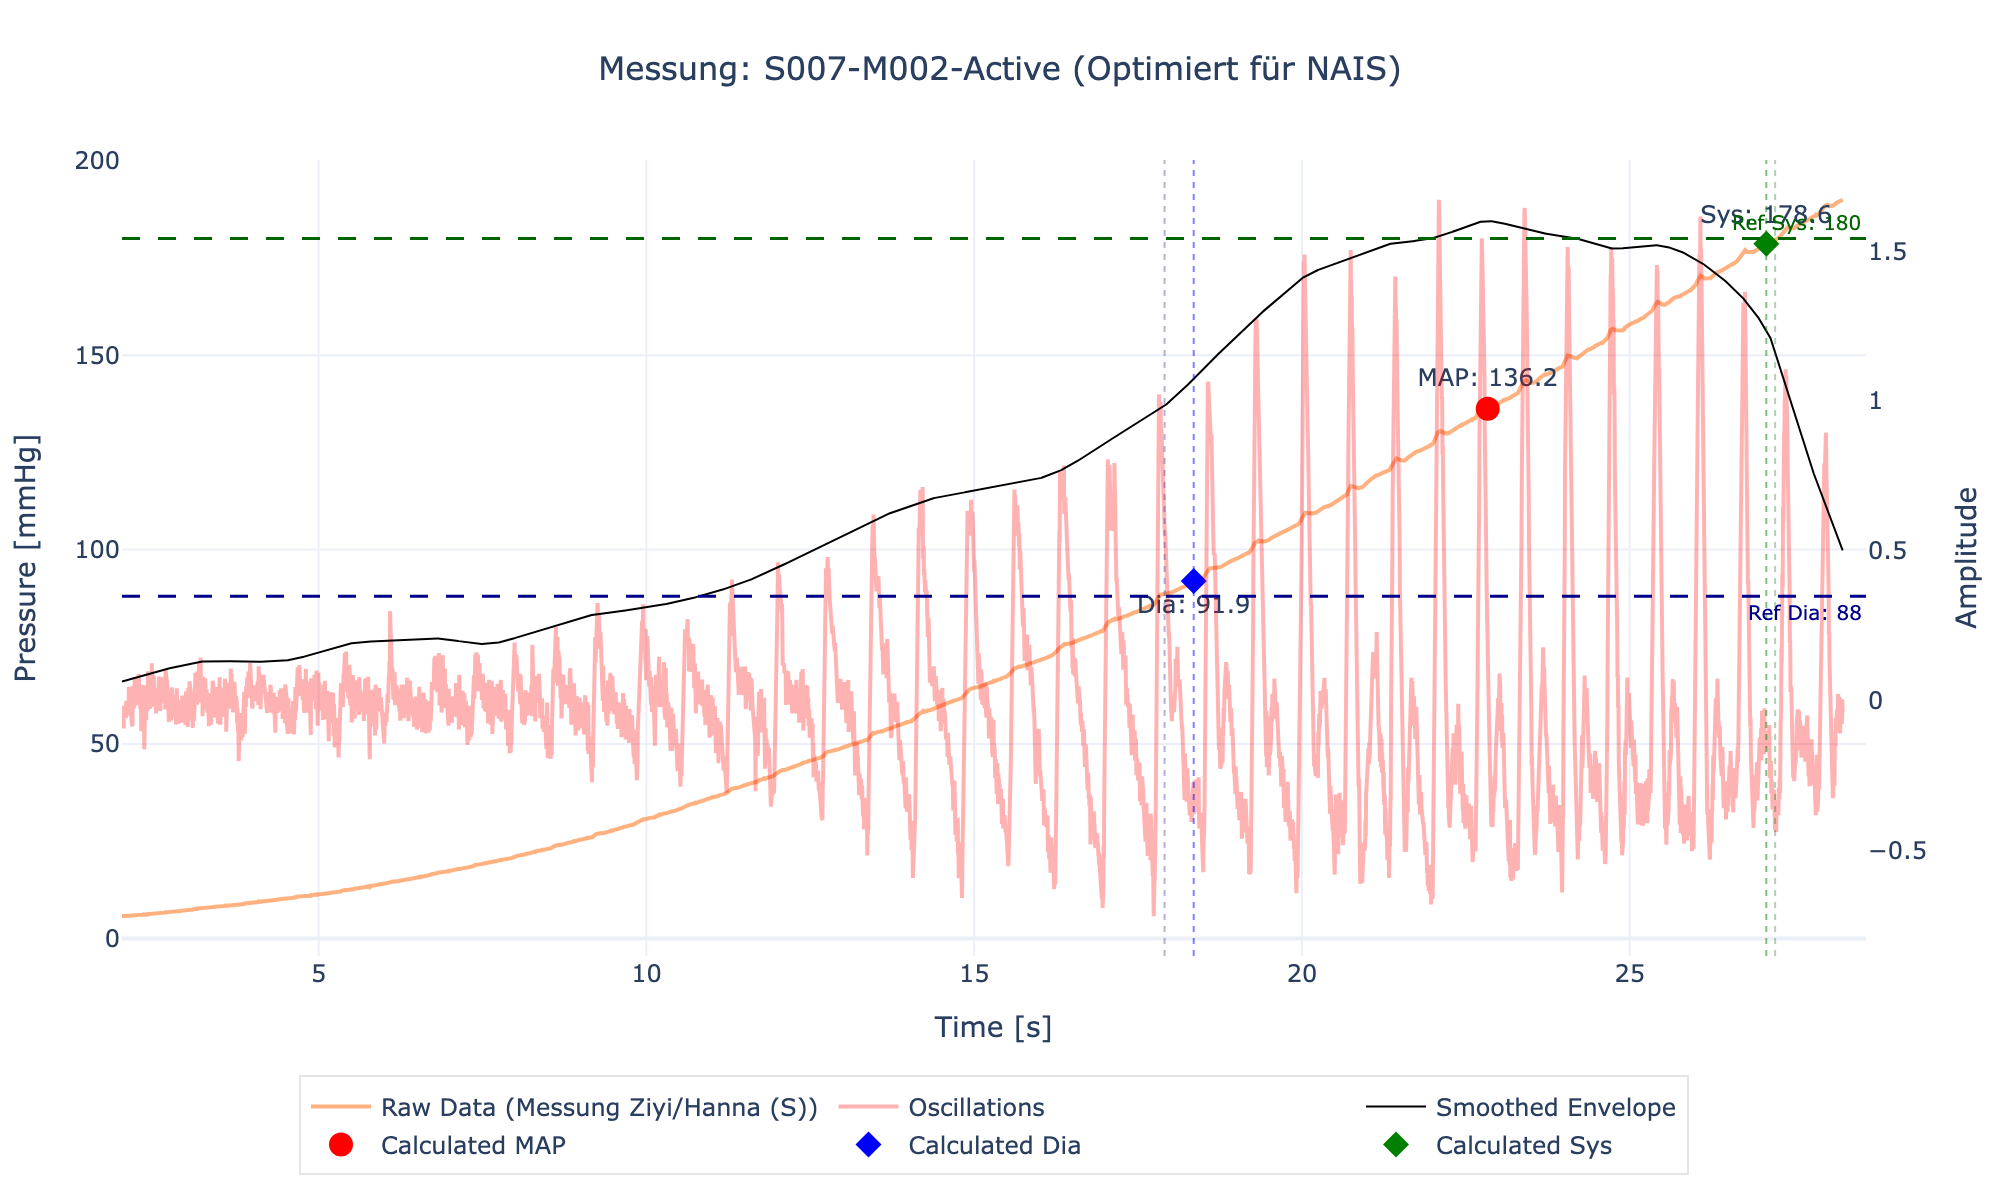
\includegraphics[width=\textwidth]{images/S007-M002-Active_nais.png}
        \caption{Optimiert für NAIS}
    \end{subfigure}
    \caption{Einzelauswertung der Messung S007-M002-Active mit verschiedenen Parametersätzen.}
\end{figure}
\newpage

\subsection*{Messung: S008-M001-Rest}
\begin{figure}[H]
    \centering
    \begin{subfigure}[b]{0.8\textwidth}
        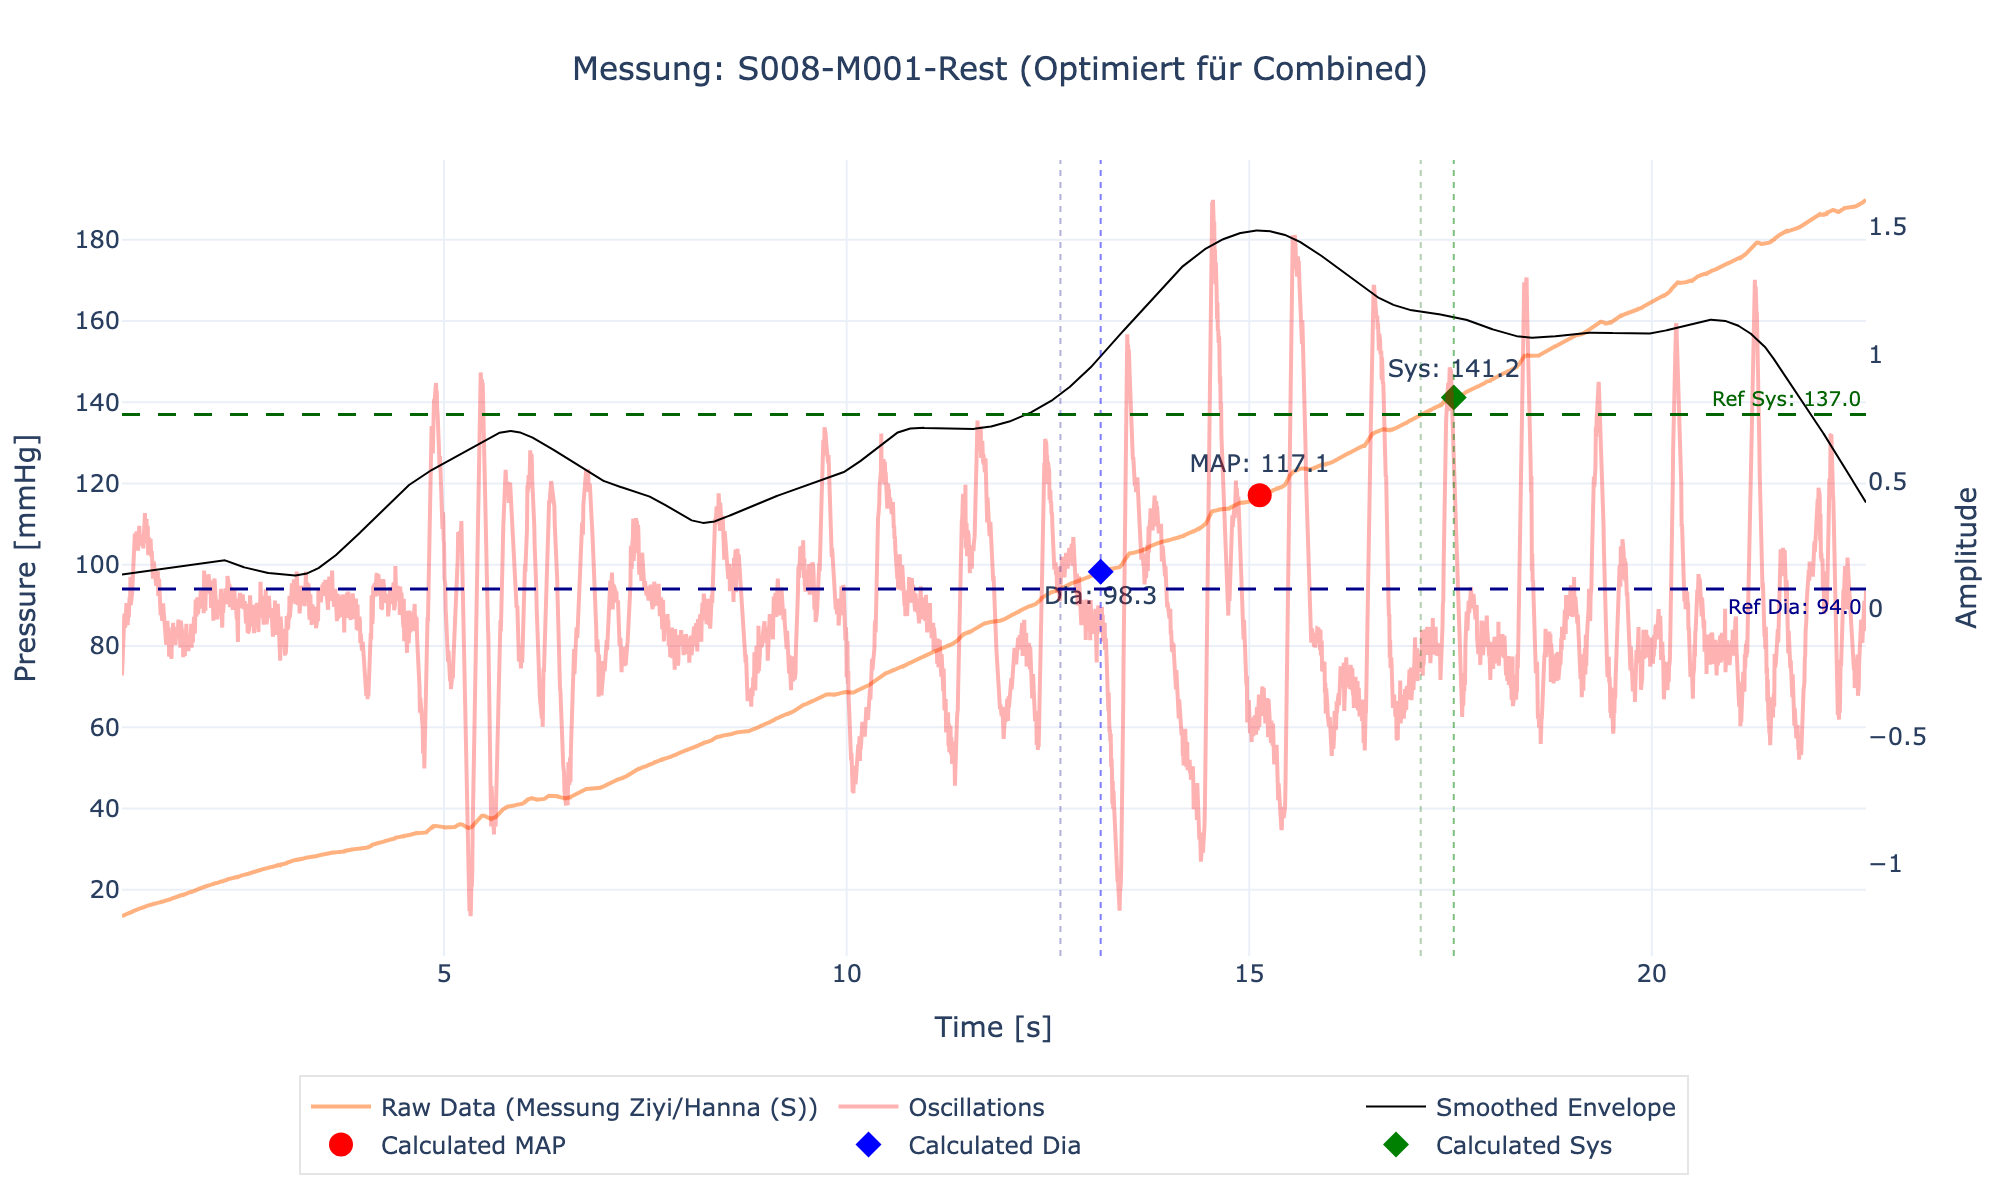
\includegraphics[width=\textwidth]{images/S008-M001-Rest_combined.png}
        \caption{Optimiert für Beurer und NAIS (Kombiniert)}
    \end{subfigure} \\
    \begin{subfigure}[b]{0.48\textwidth}
        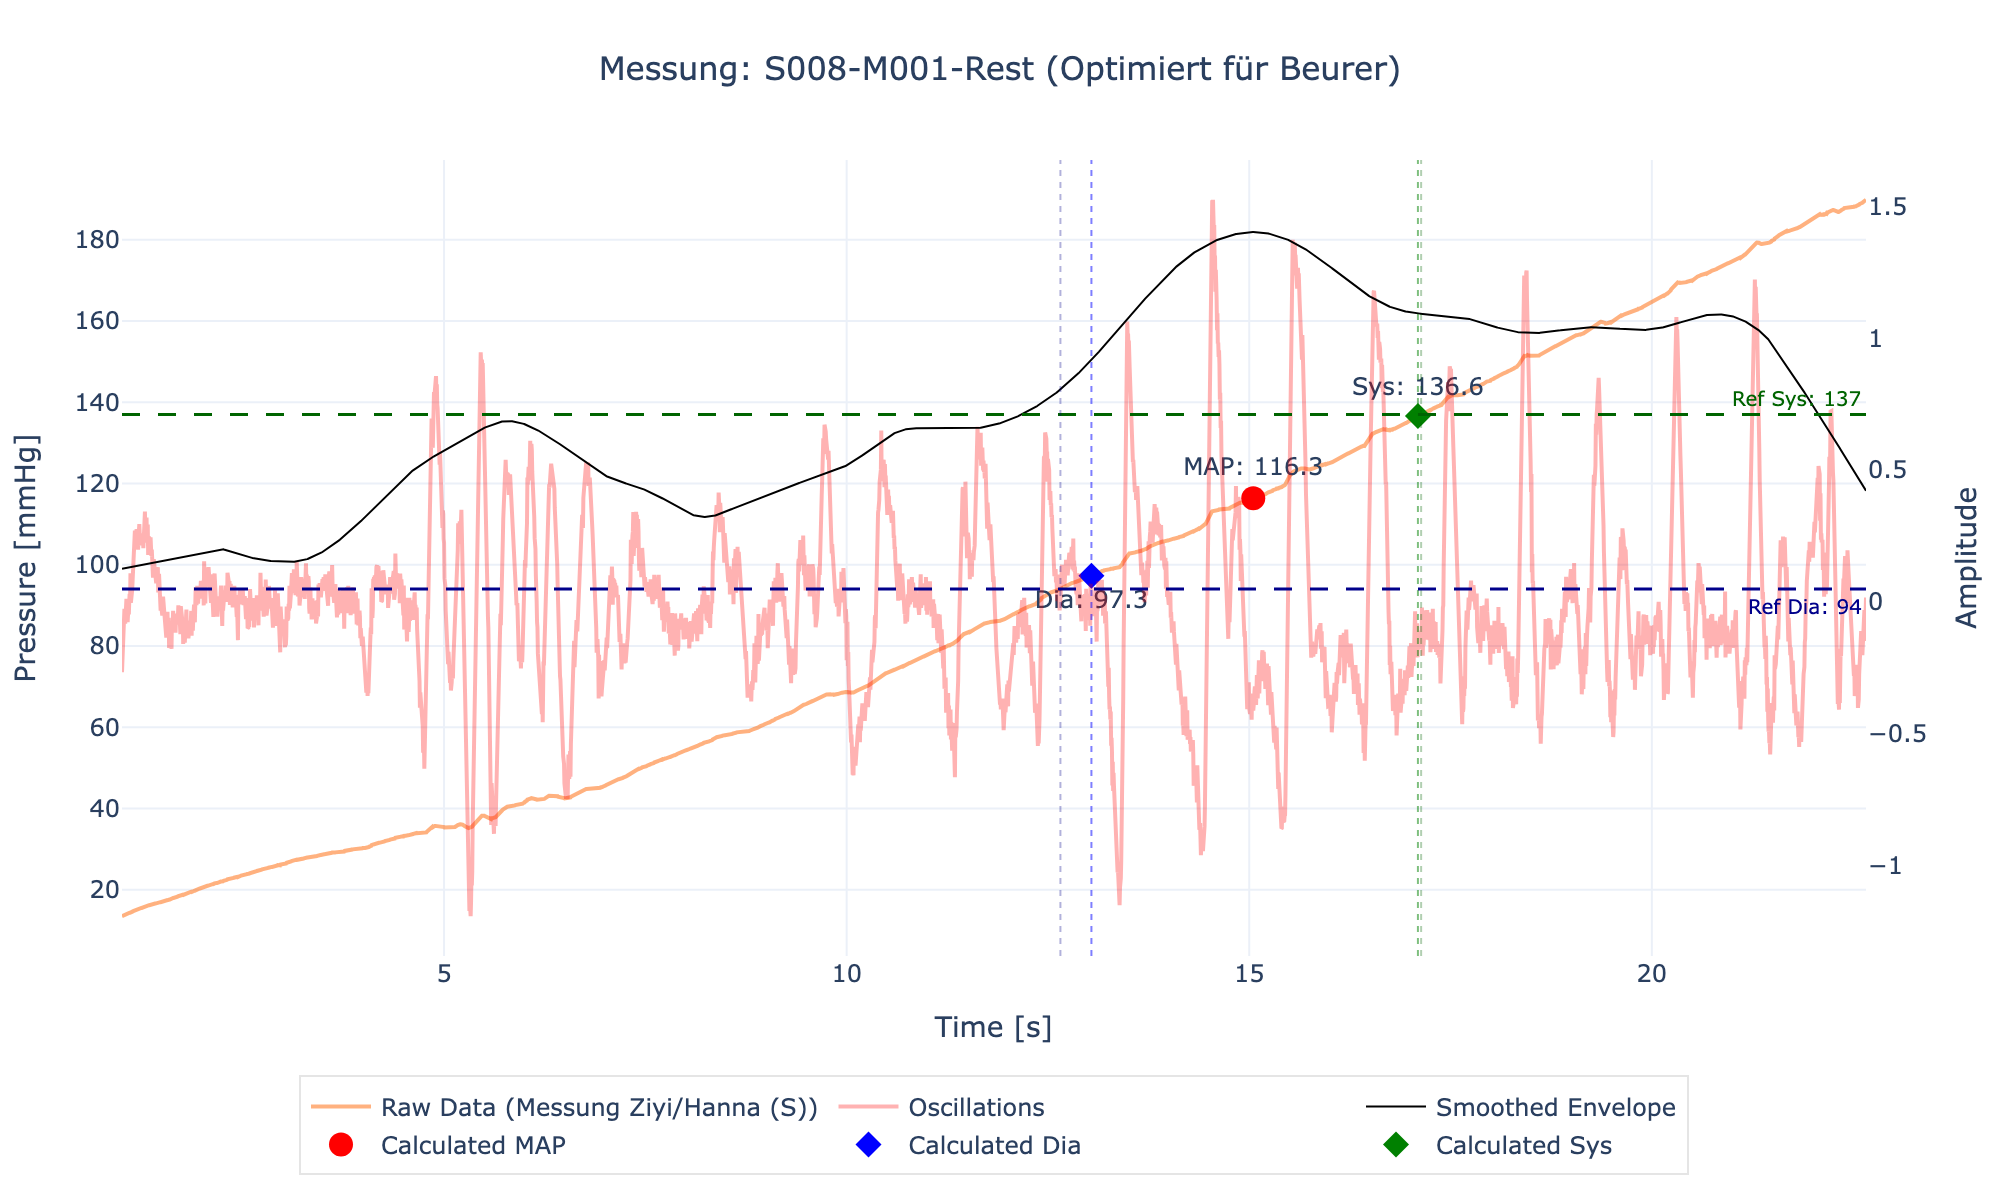
\includegraphics[width=\textwidth]{images/S008-M001-Rest_beurer.png}
        \caption{Optimiert für Beurer}
    \end{subfigure}
    \hfill
    \begin{subfigure}[b]{0.48\textwidth}
        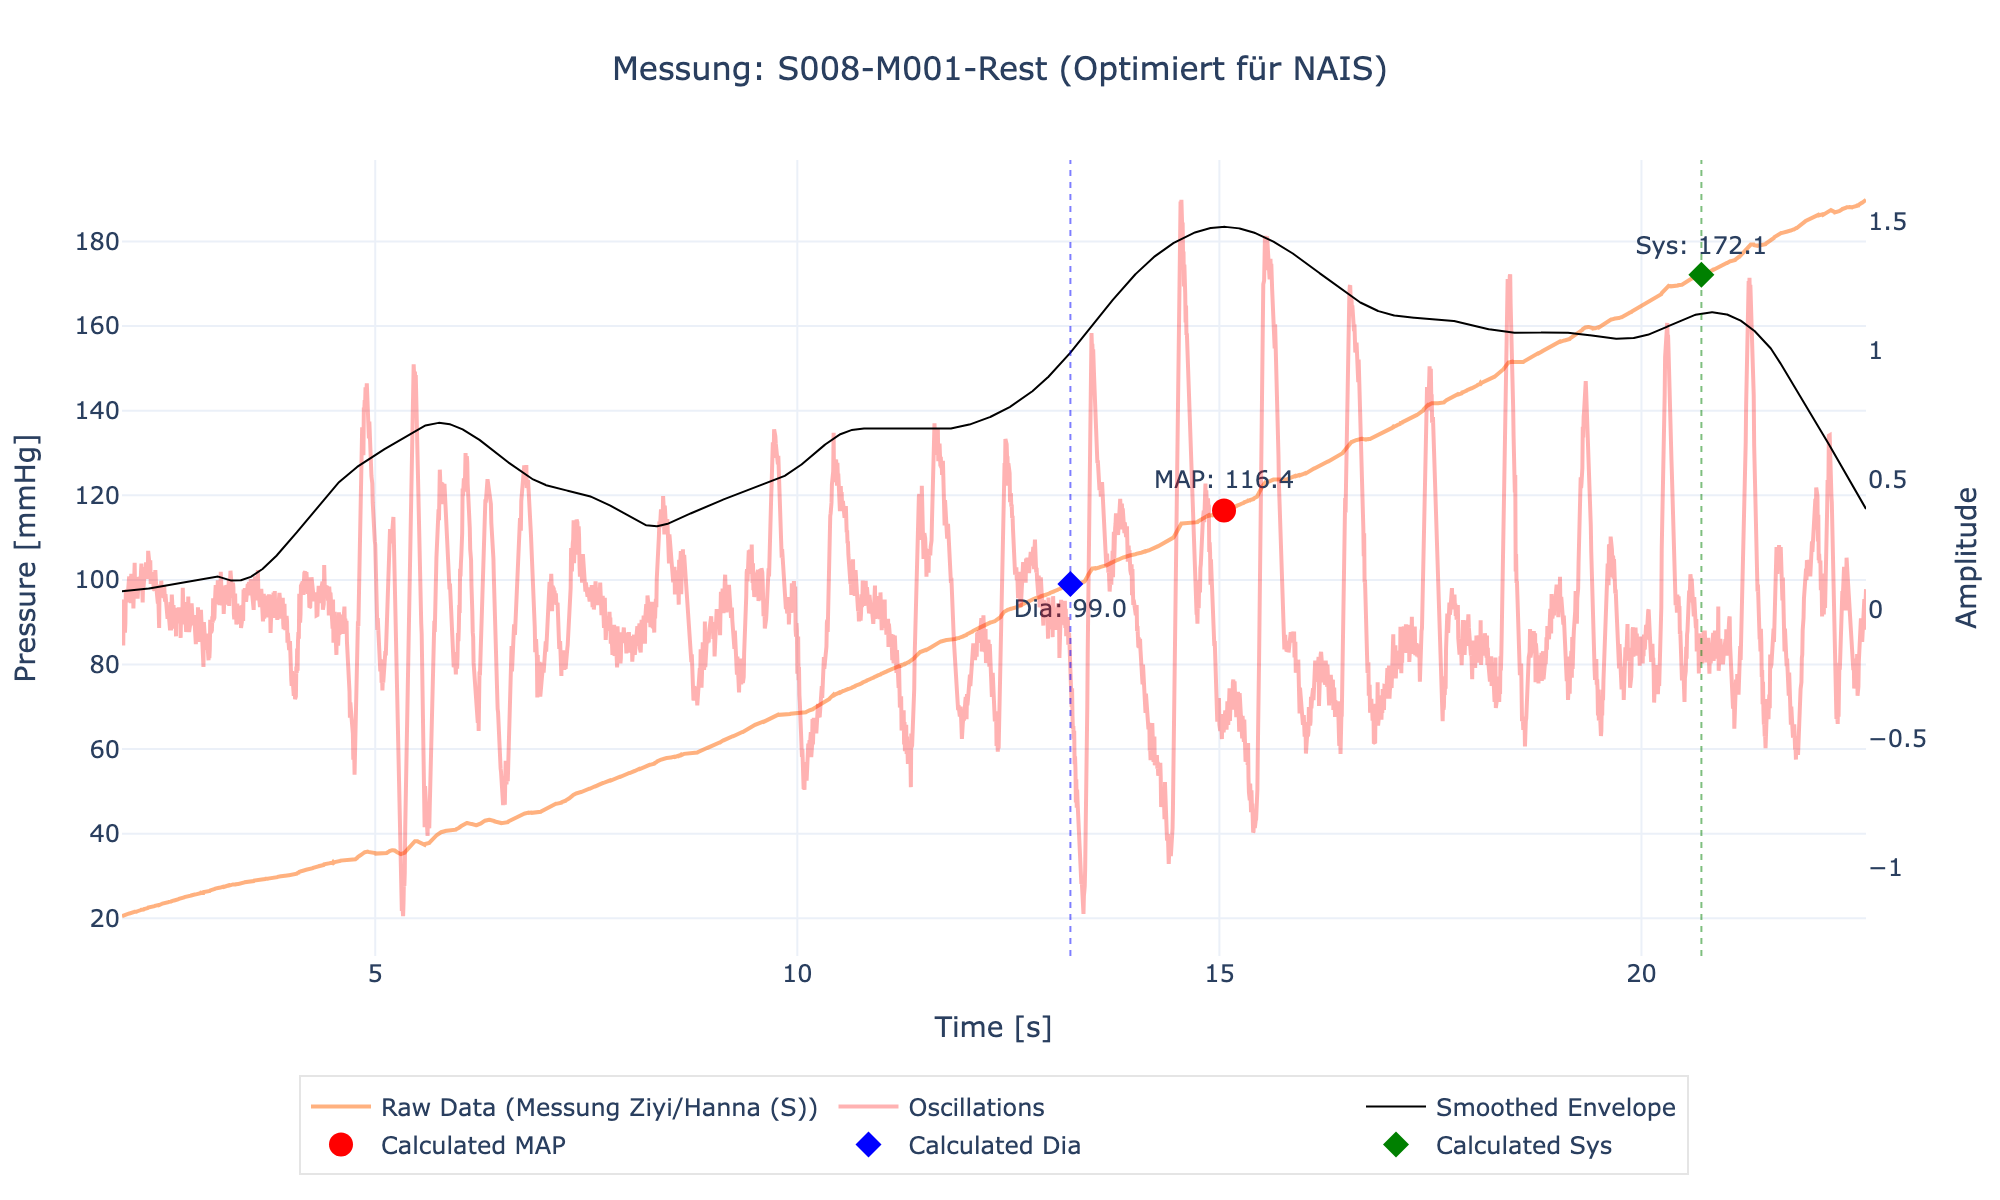
\includegraphics[width=\textwidth]{images/S008-M001-Rest_nais.png}
        \caption{Optimiert für NAIS}
    \end{subfigure}
    \caption{Einzelauswertung der Messung S008-M001-Rest mit verschiedenen Parametersätzen.}
\end{figure}
\newpage

\subsection*{Messung: S008-M002-Active}
\begin{figure}[H]
    \centering
    \begin{subfigure}[b]{0.8\textwidth}
        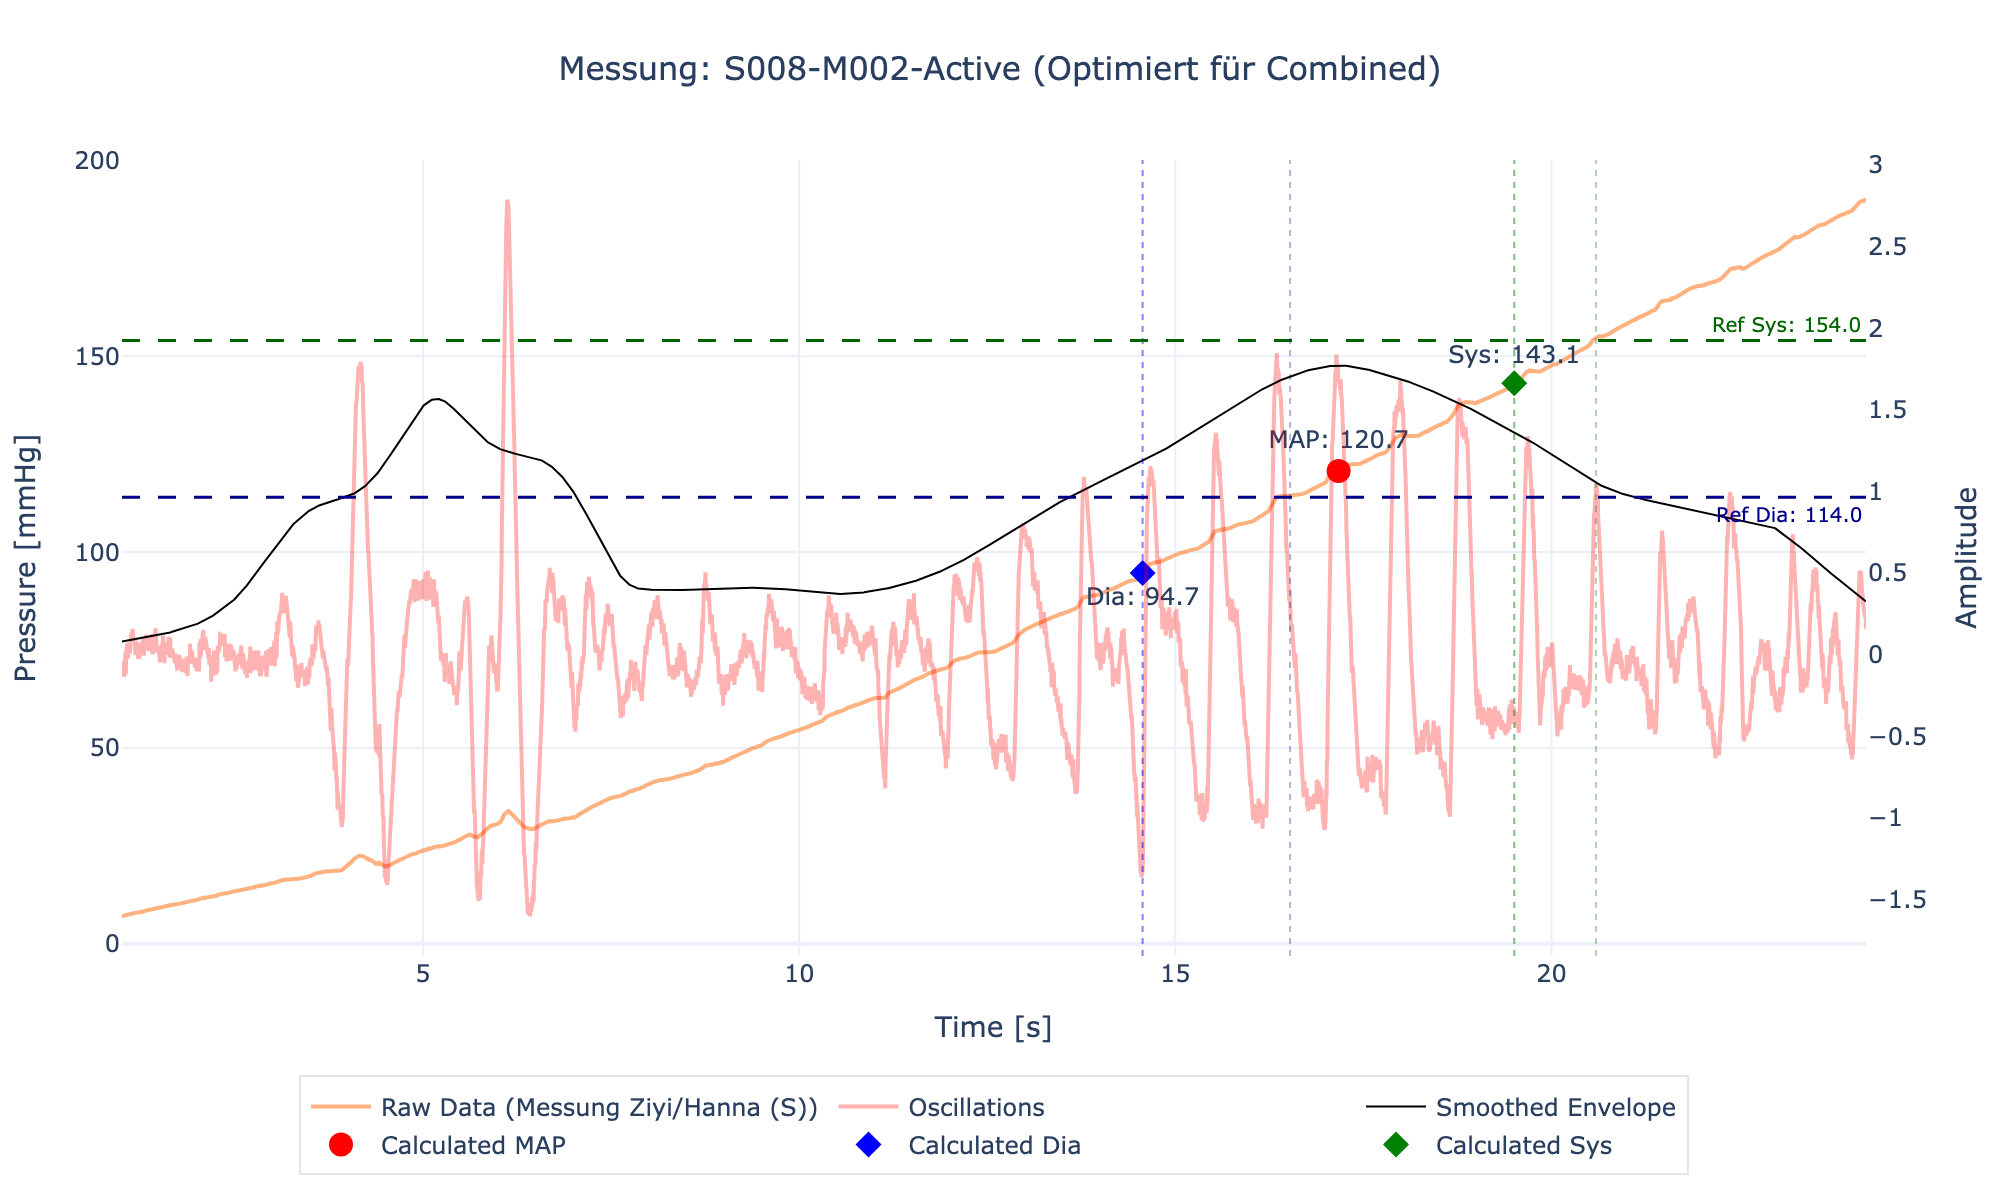
\includegraphics[width=\textwidth]{images/S008-M002-Active_combined.png}
        \caption{Optimiert für Beurer und NAIS (Kombiniert)}
    \end{subfigure} \\
    \begin{subfigure}[b]{0.48\textwidth}
        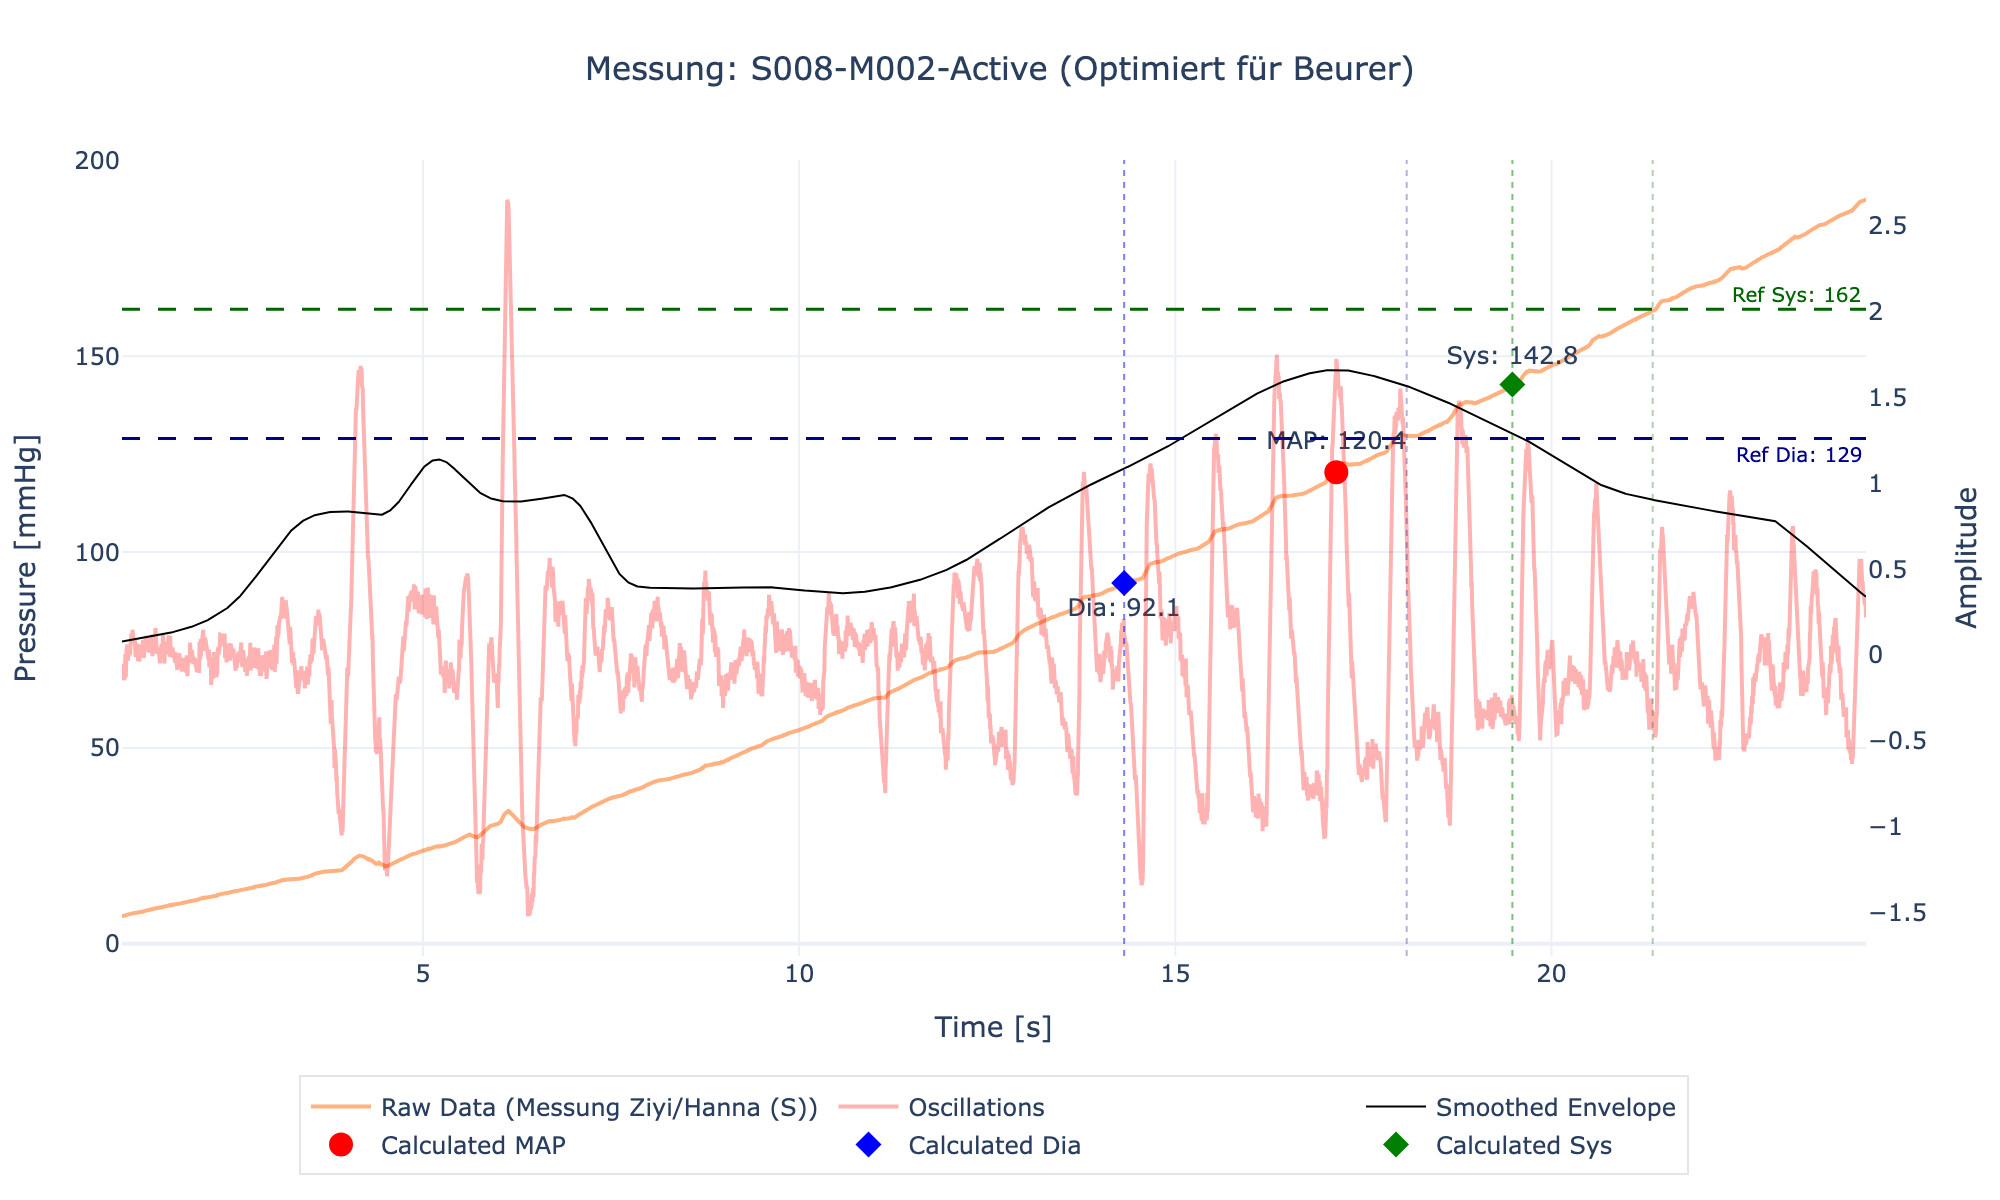
\includegraphics[width=\textwidth]{images/S008-M002-Active_beurer.png}
        \caption{Optimiert für Beurer}
    \end{subfigure}
    \hfill
    \begin{subfigure}[b]{0.48\textwidth}
        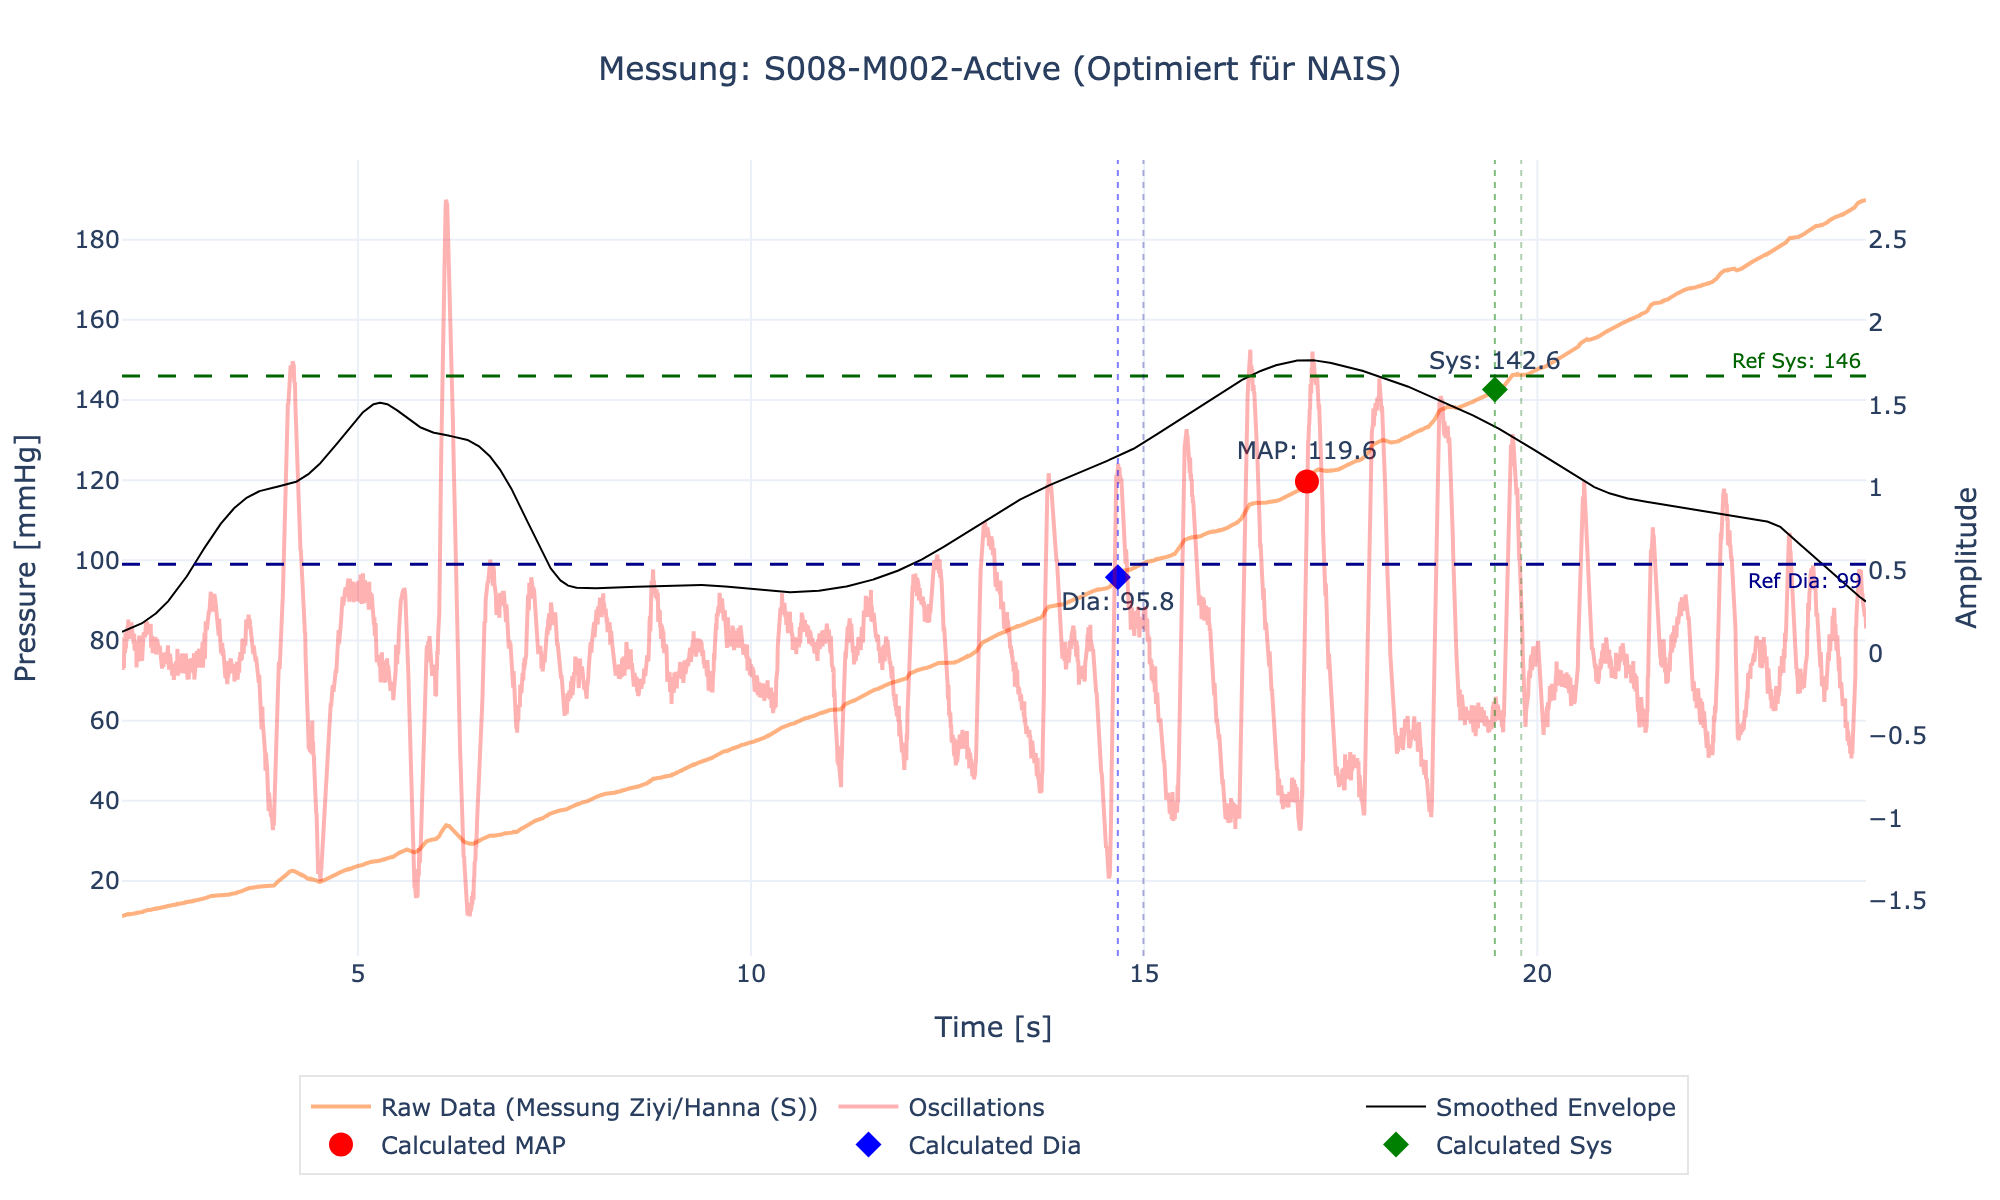
\includegraphics[width=\textwidth]{images/S008-M002-Active_nais.png}
        \caption{Optimiert für NAIS}
    \end{subfigure}
    \caption{Einzelauswertung der Messung S008-M002-Active mit verschiedenen Parametersätzen.}
\end{figure}
\newpage

\subsection*{Messung: S009-M001-Rest}
\begin{figure}[H]
    \centering
    \begin{subfigure}[b]{0.8\textwidth}
        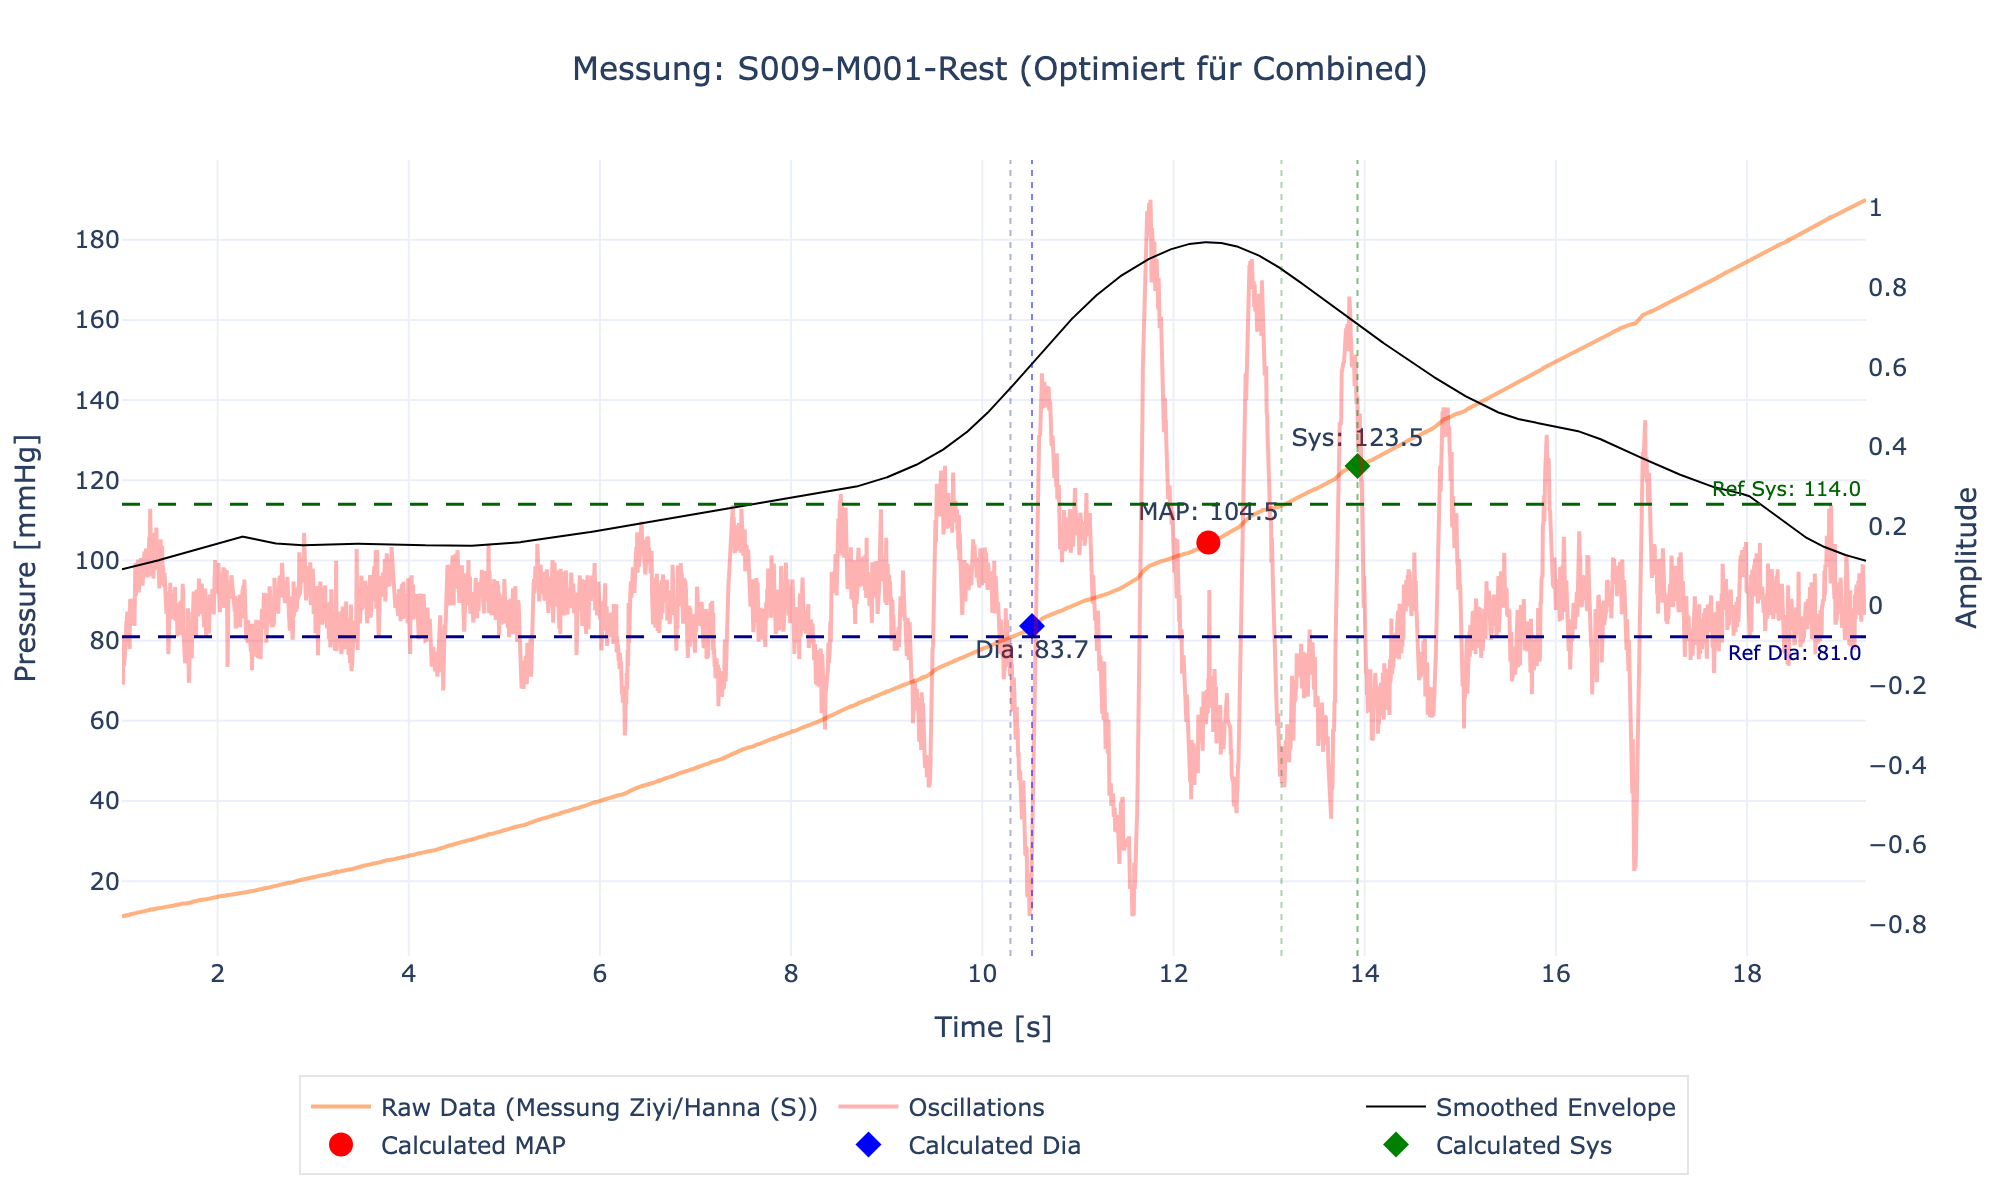
\includegraphics[width=\textwidth]{images/S009-M001-Rest_combined.png}
        \caption{Optimiert für Beurer und NAIS (Kombiniert)}
    \end{subfigure} \\
    \begin{subfigure}[b]{0.48\textwidth}
        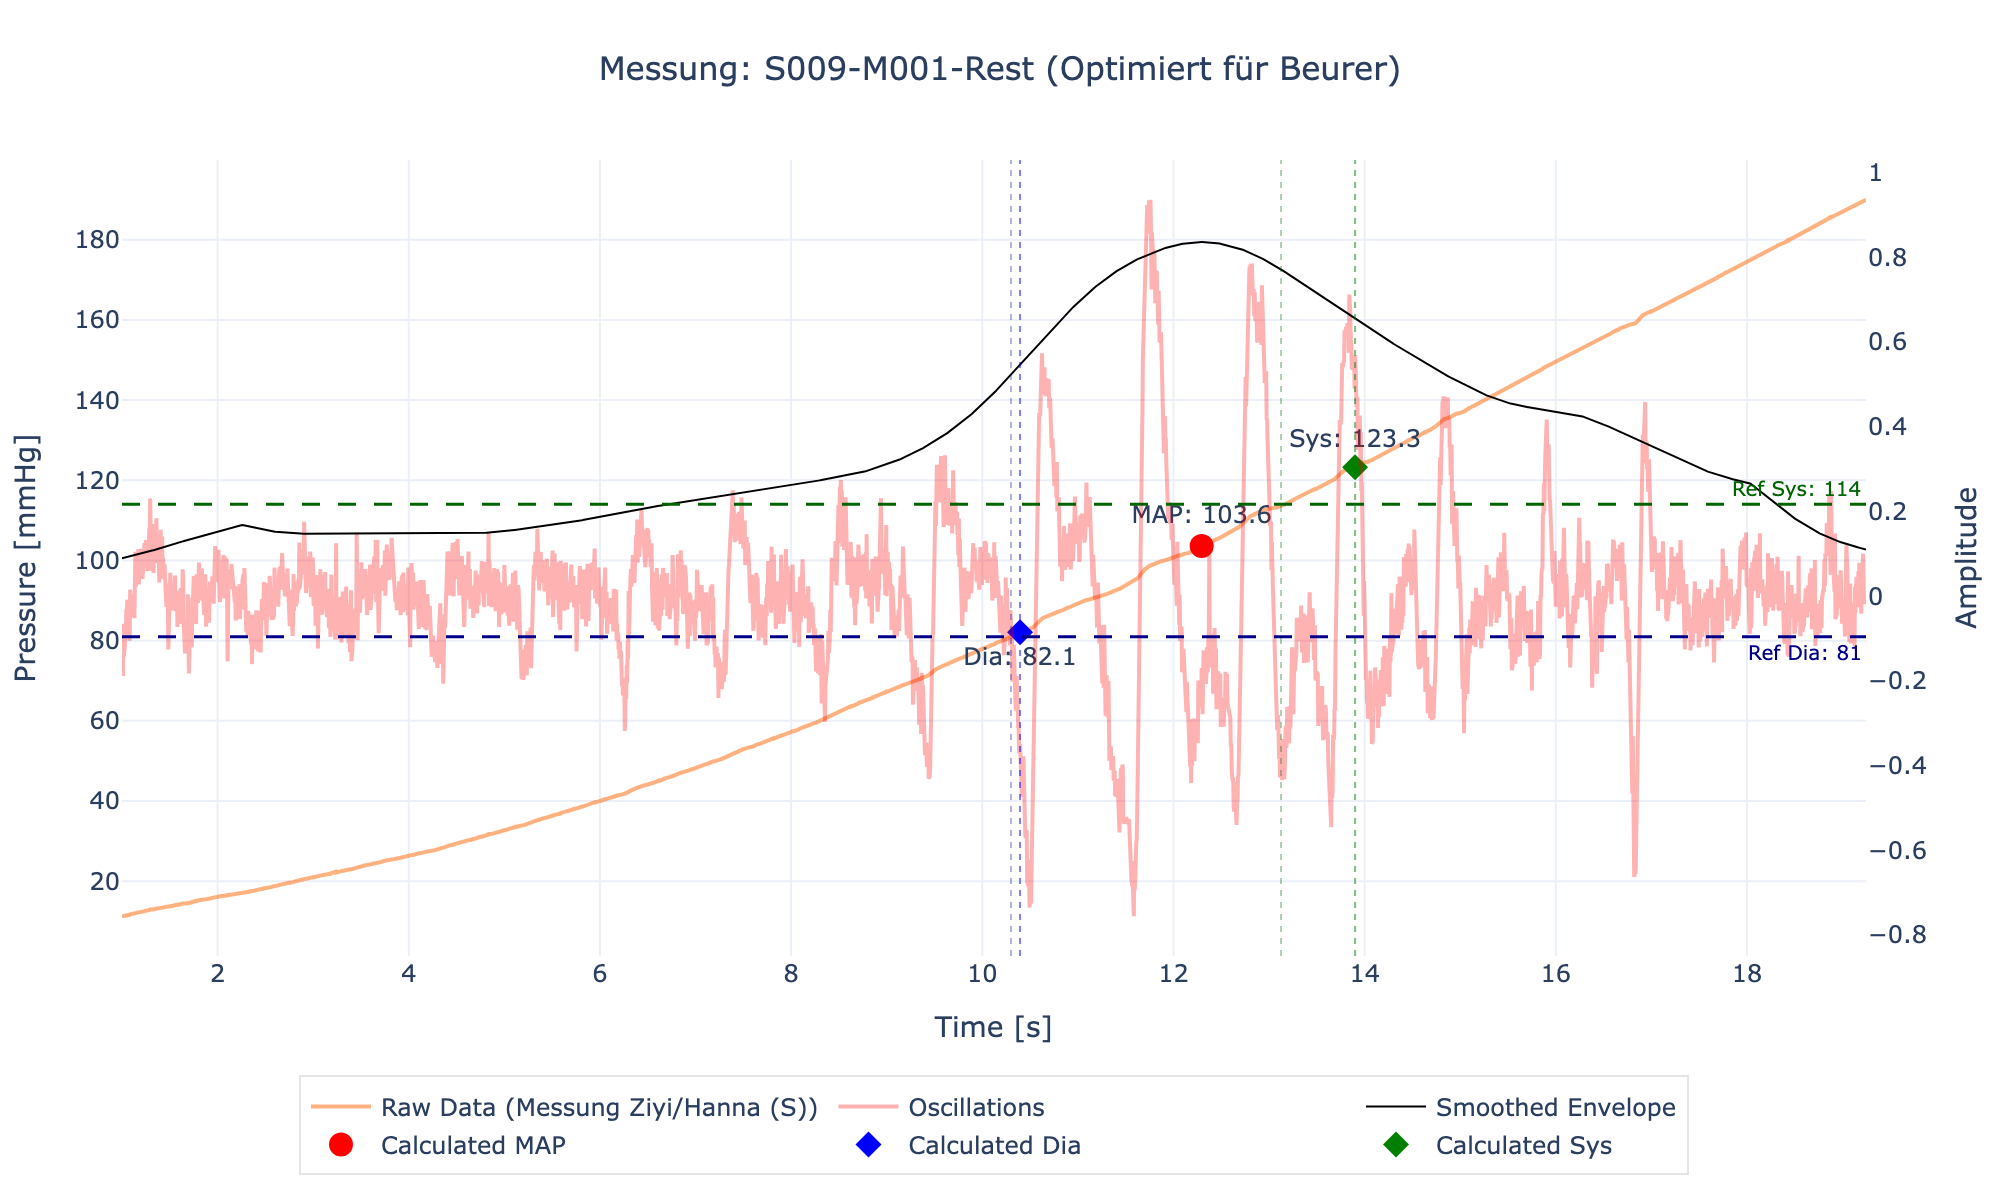
\includegraphics[width=\textwidth]{images/S009-M001-Rest_beurer.png}
        \caption{Optimiert für Beurer}
    \end{subfigure}
    \hfill
    \begin{subfigure}[b]{0.48\textwidth}
        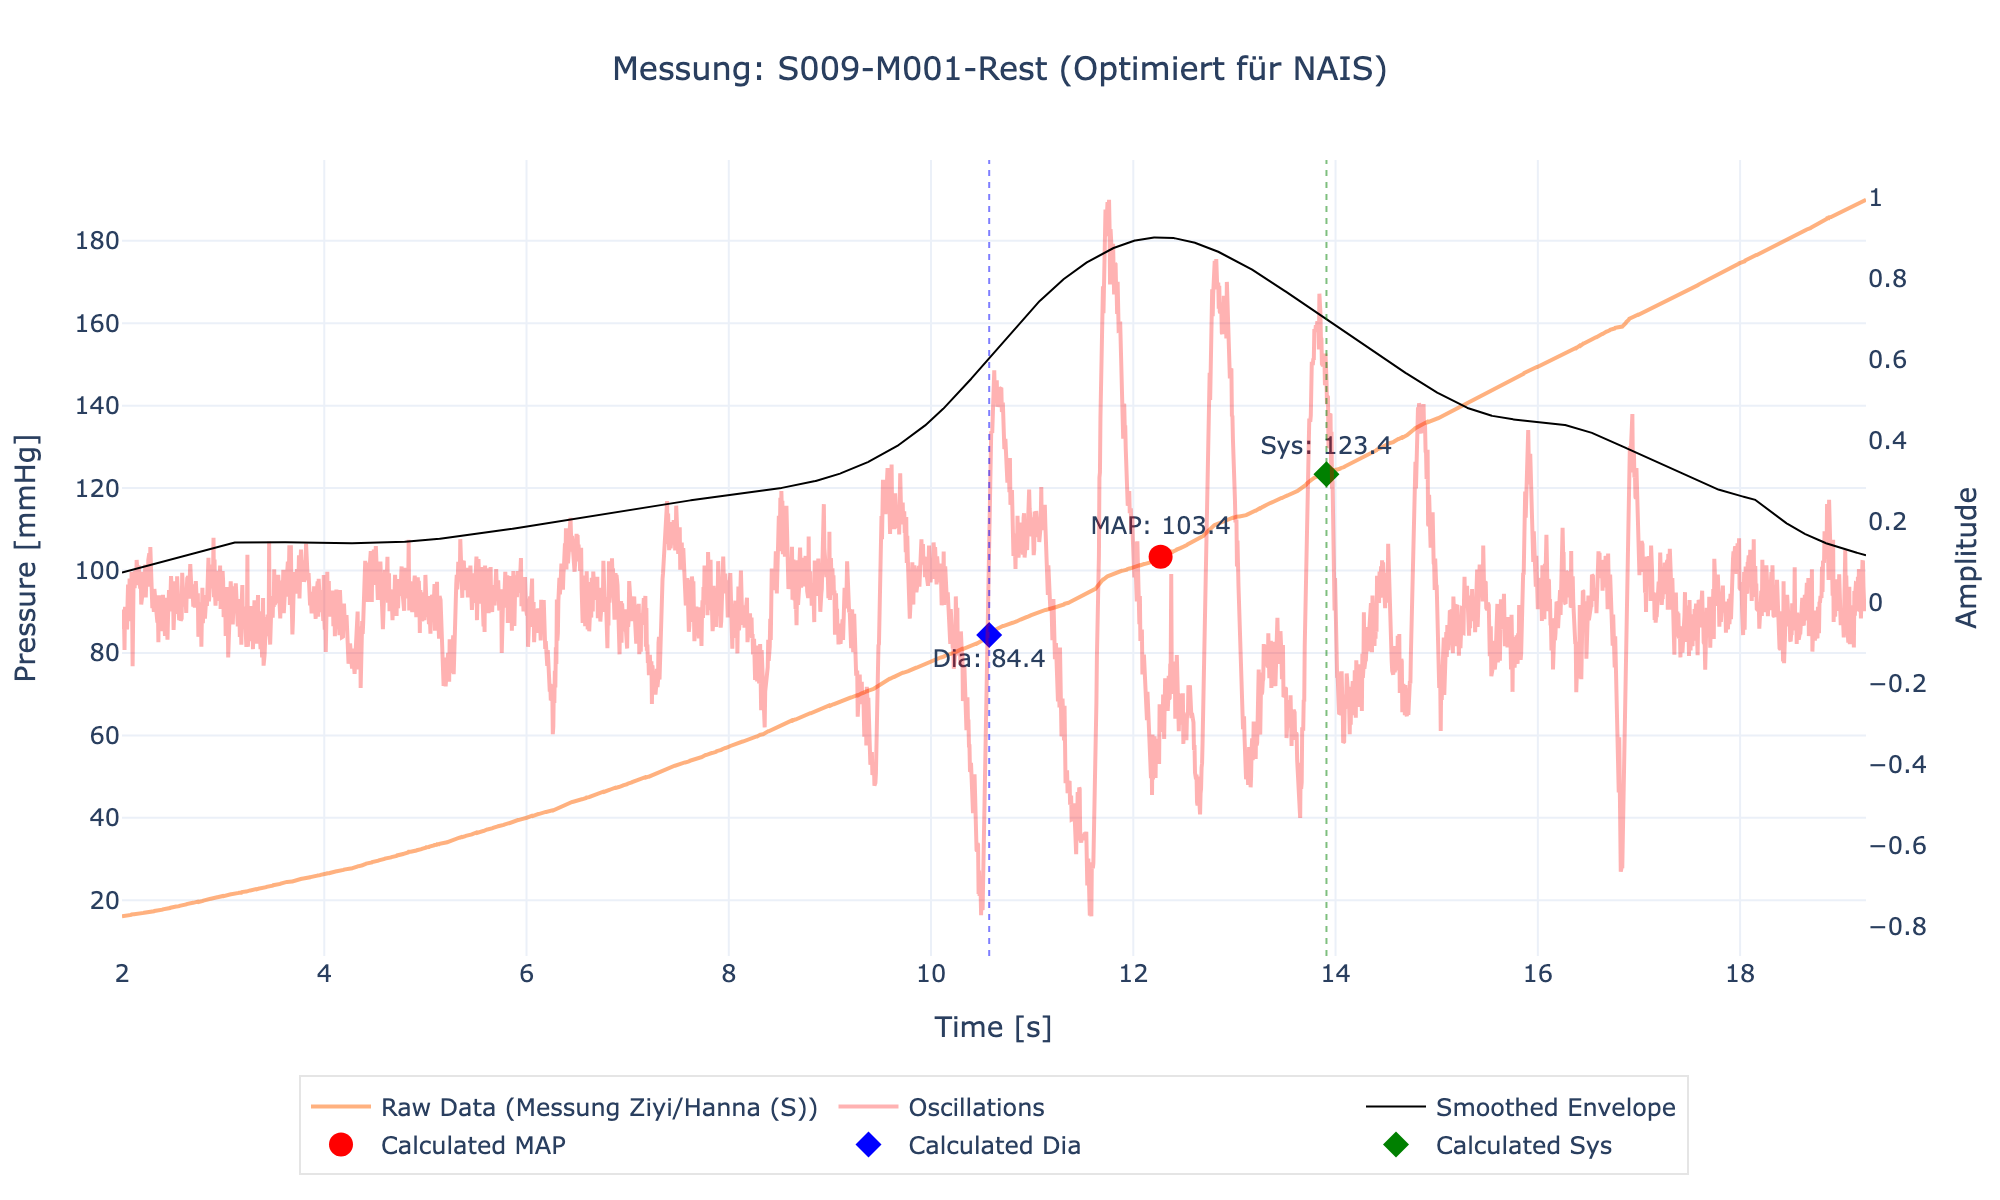
\includegraphics[width=\textwidth]{images/S009-M001-Rest_nais.png}
        \caption{Optimiert für NAIS}
    \end{subfigure}
    \caption{Einzelauswertung der Messung S009-M001-Rest mit verschiedenen Parametersätzen.}
\end{figure}
\newpage

\subsection*{Messung: S009-M002-Active}
\begin{figure}[H]
    \centering
    \begin{subfigure}[b]{0.8\textwidth}
        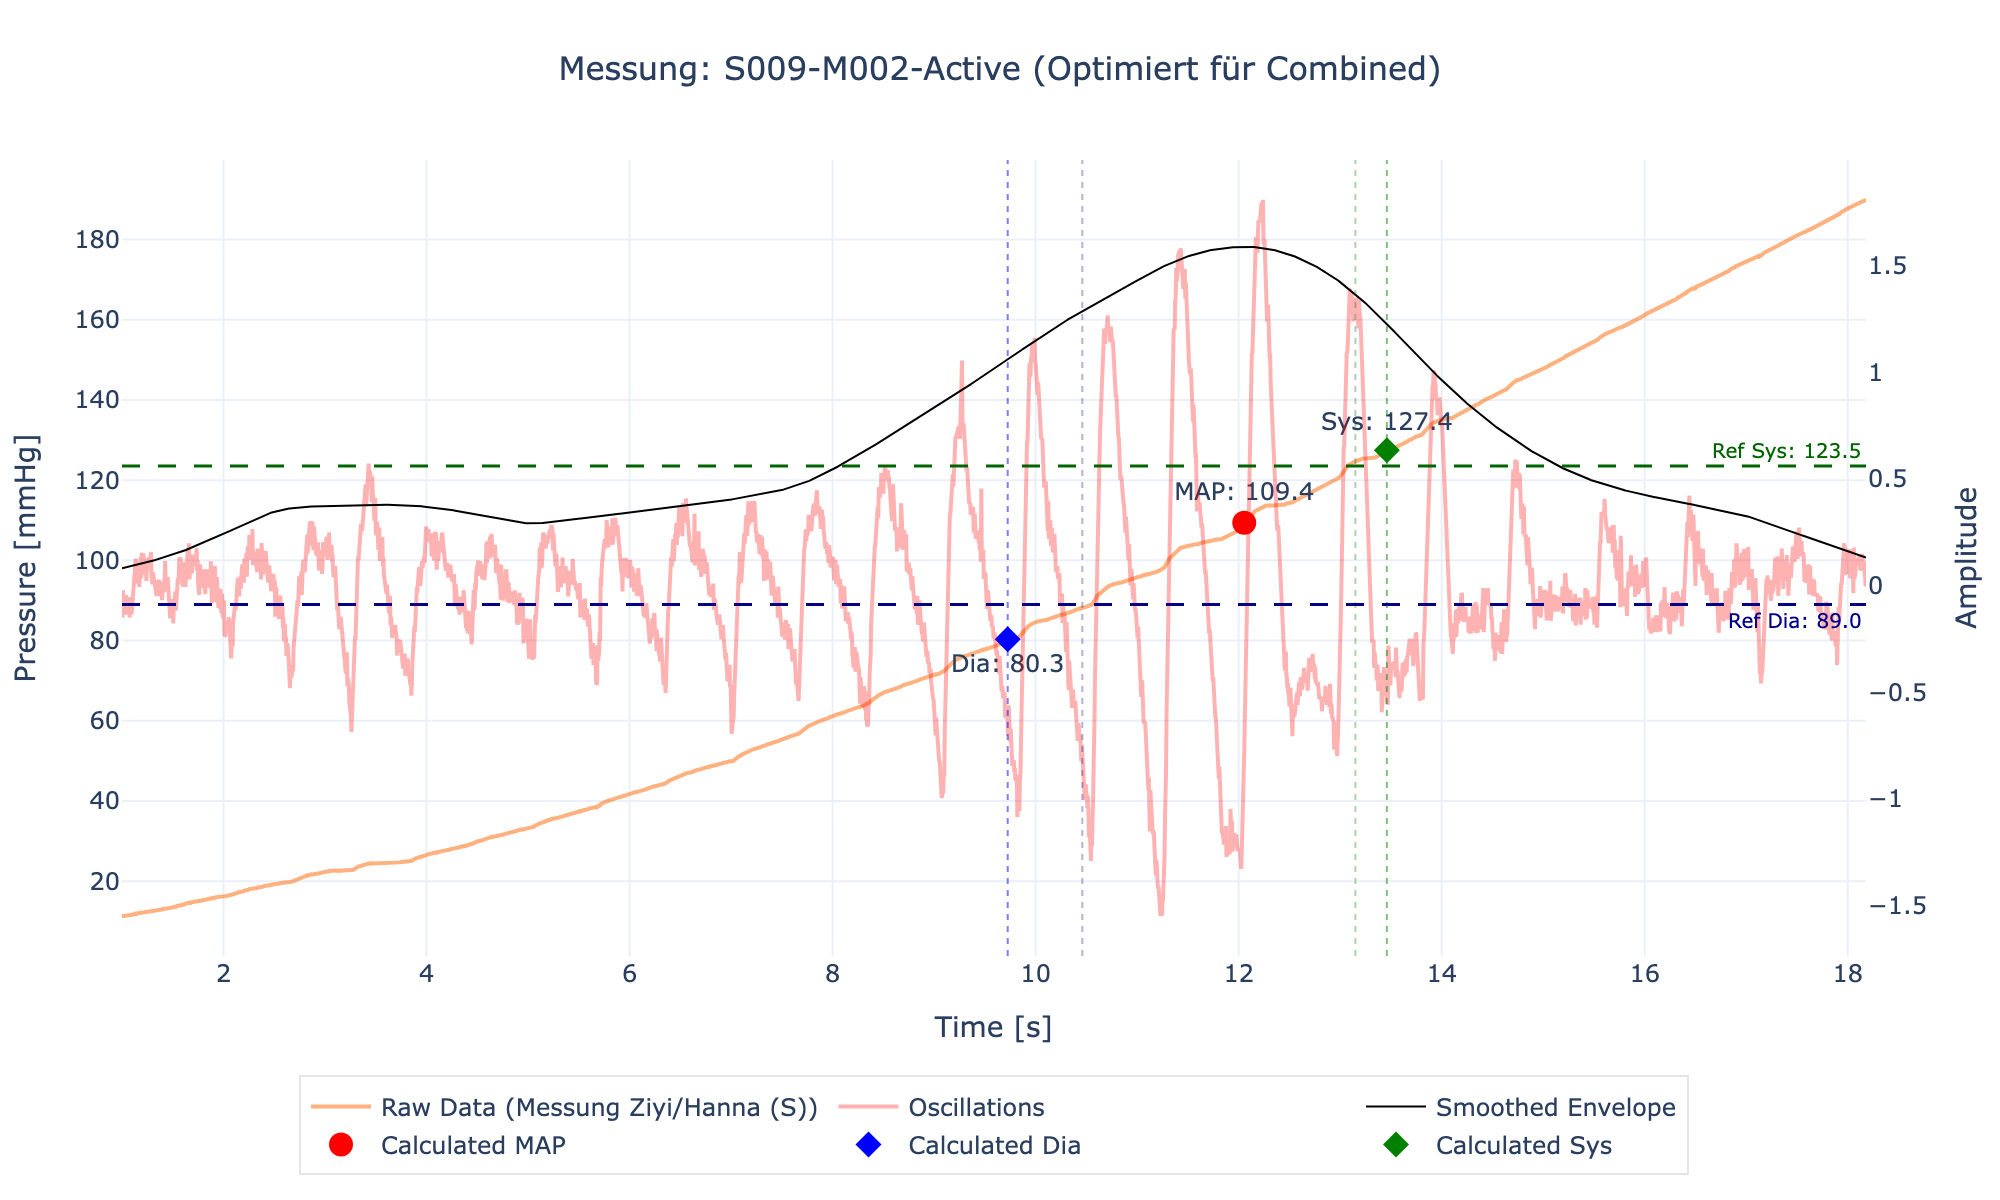
\includegraphics[width=\textwidth]{images/S009-M002-Active_combined.png}
        \caption{Optimiert für Beurer und NAIS (Kombiniert)}
    \end{subfigure} \\
    \begin{subfigure}[b]{0.48\textwidth}
        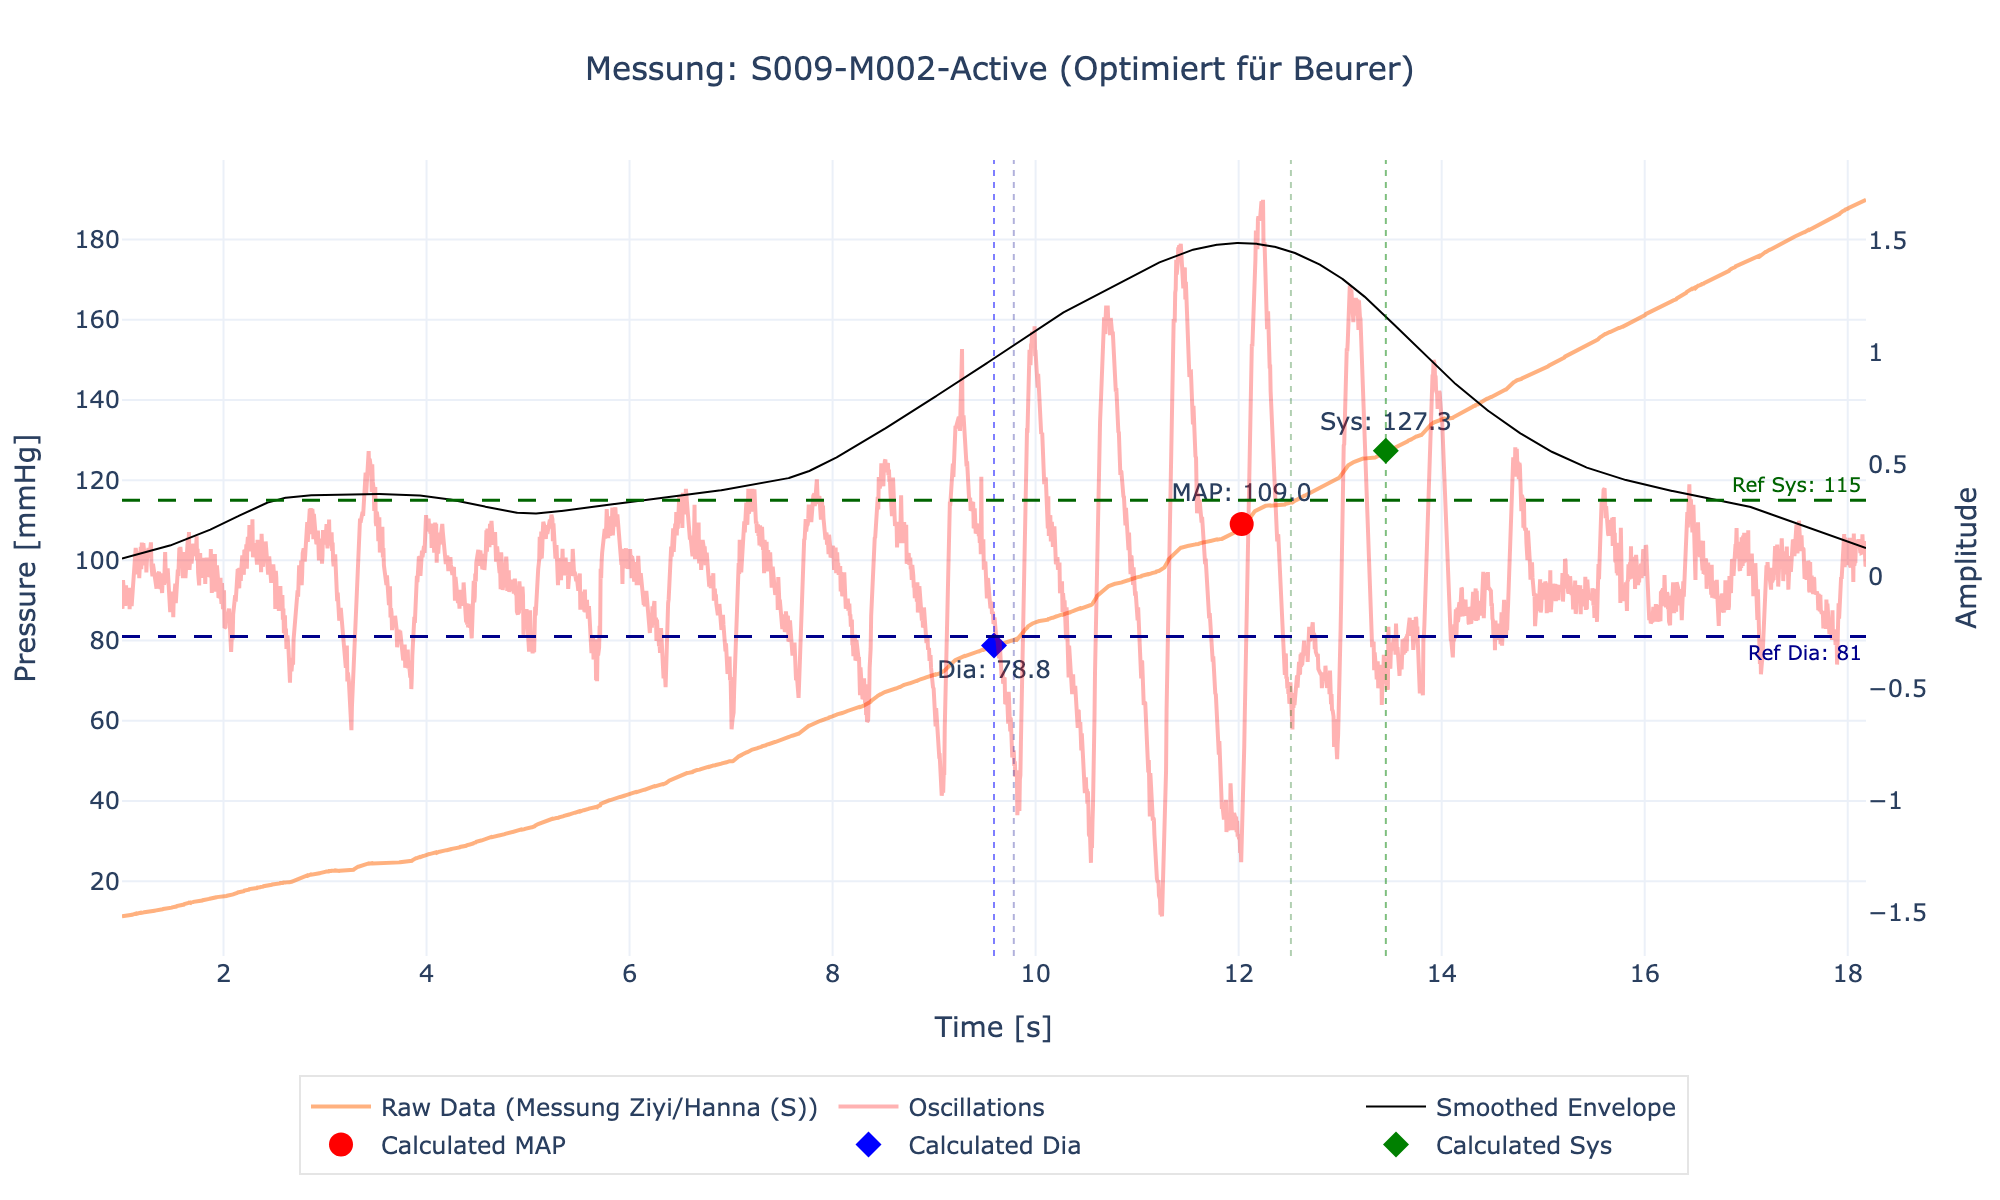
\includegraphics[width=\textwidth]{images/S009-M002-Active_beurer.png}
        \caption{Optimiert für Beurer}
    \end{subfigure}
    \hfill
    \begin{subfigure}[b]{0.48\textwidth}
        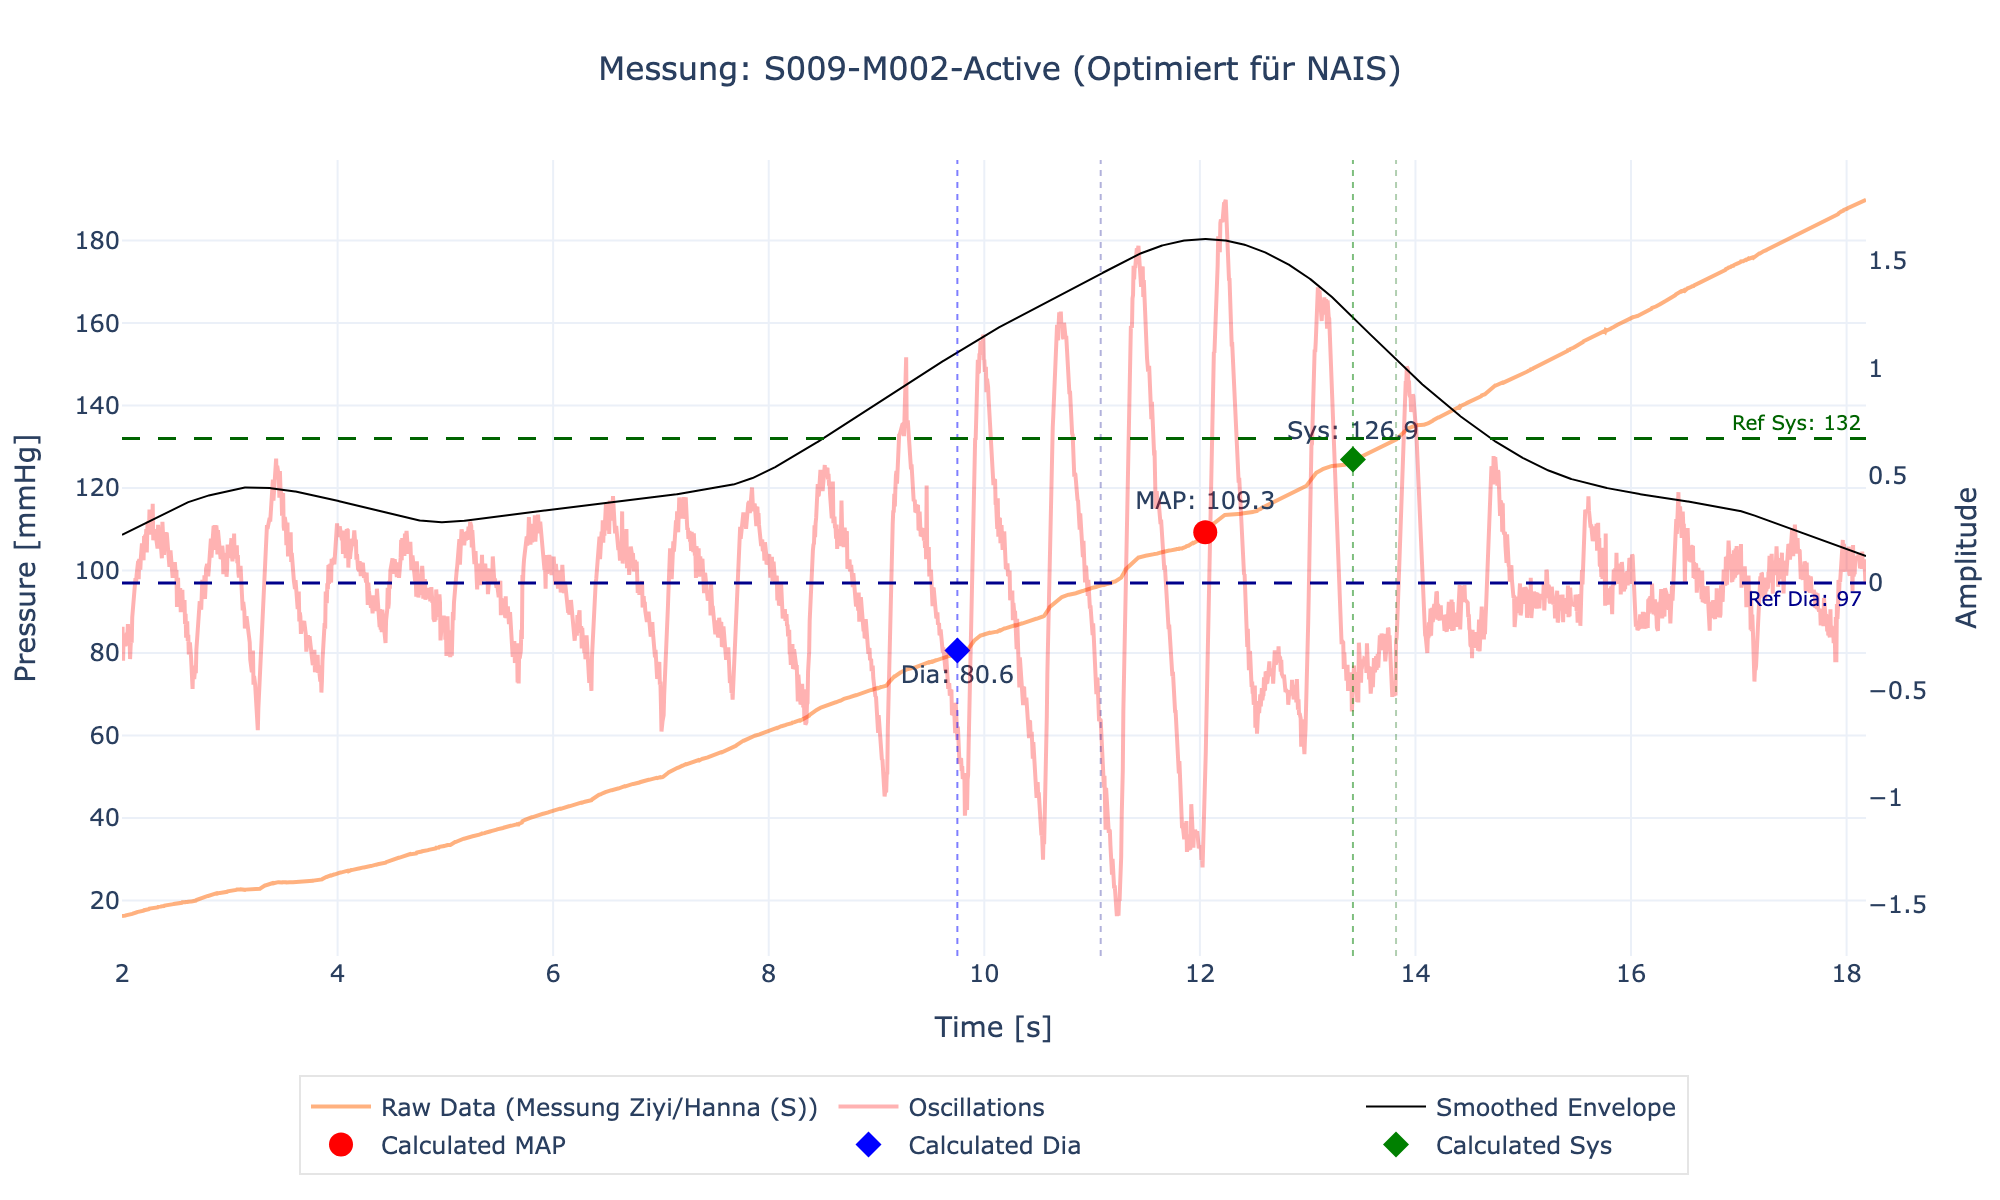
\includegraphics[width=\textwidth]{images/S009-M002-Active_nais.png}
        \caption{Optimiert für NAIS}
    \end{subfigure}
    \caption{Einzelauswertung der Messung S009-M002-Active mit verschiedenen Parametersätzen.}
\end{figure}
\newpage

\subsection*{Messung: S010-M001-Rest}
\begin{figure}[H]
    \centering
    \begin{subfigure}[b]{0.8\textwidth}
        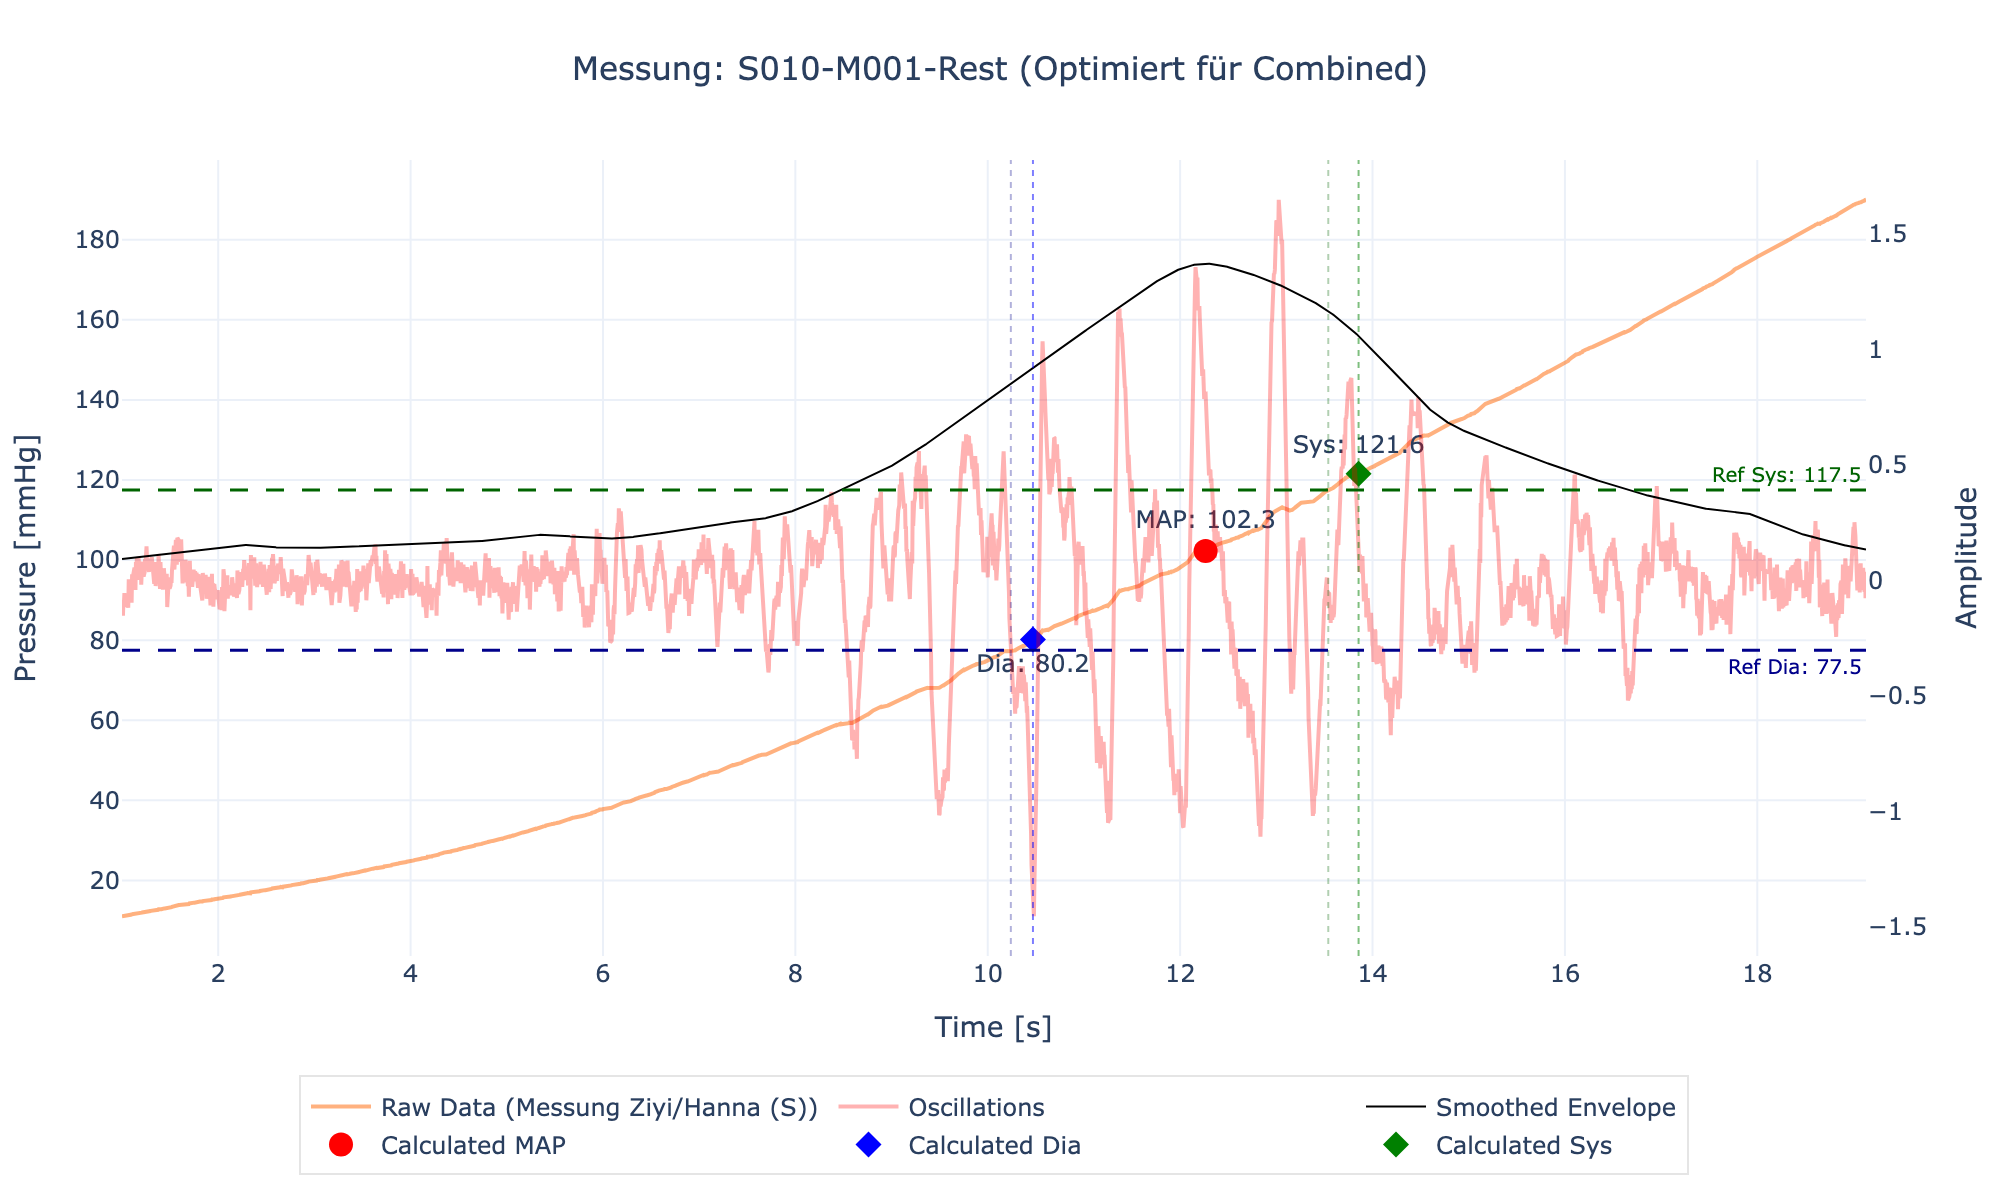
\includegraphics[width=\textwidth]{images/S010-M001-Rest_combined.png}
        \caption{Optimiert für Beurer und NAIS (Kombiniert)}
    \end{subfigure} \\
    \begin{subfigure}[b]{0.48\textwidth}
        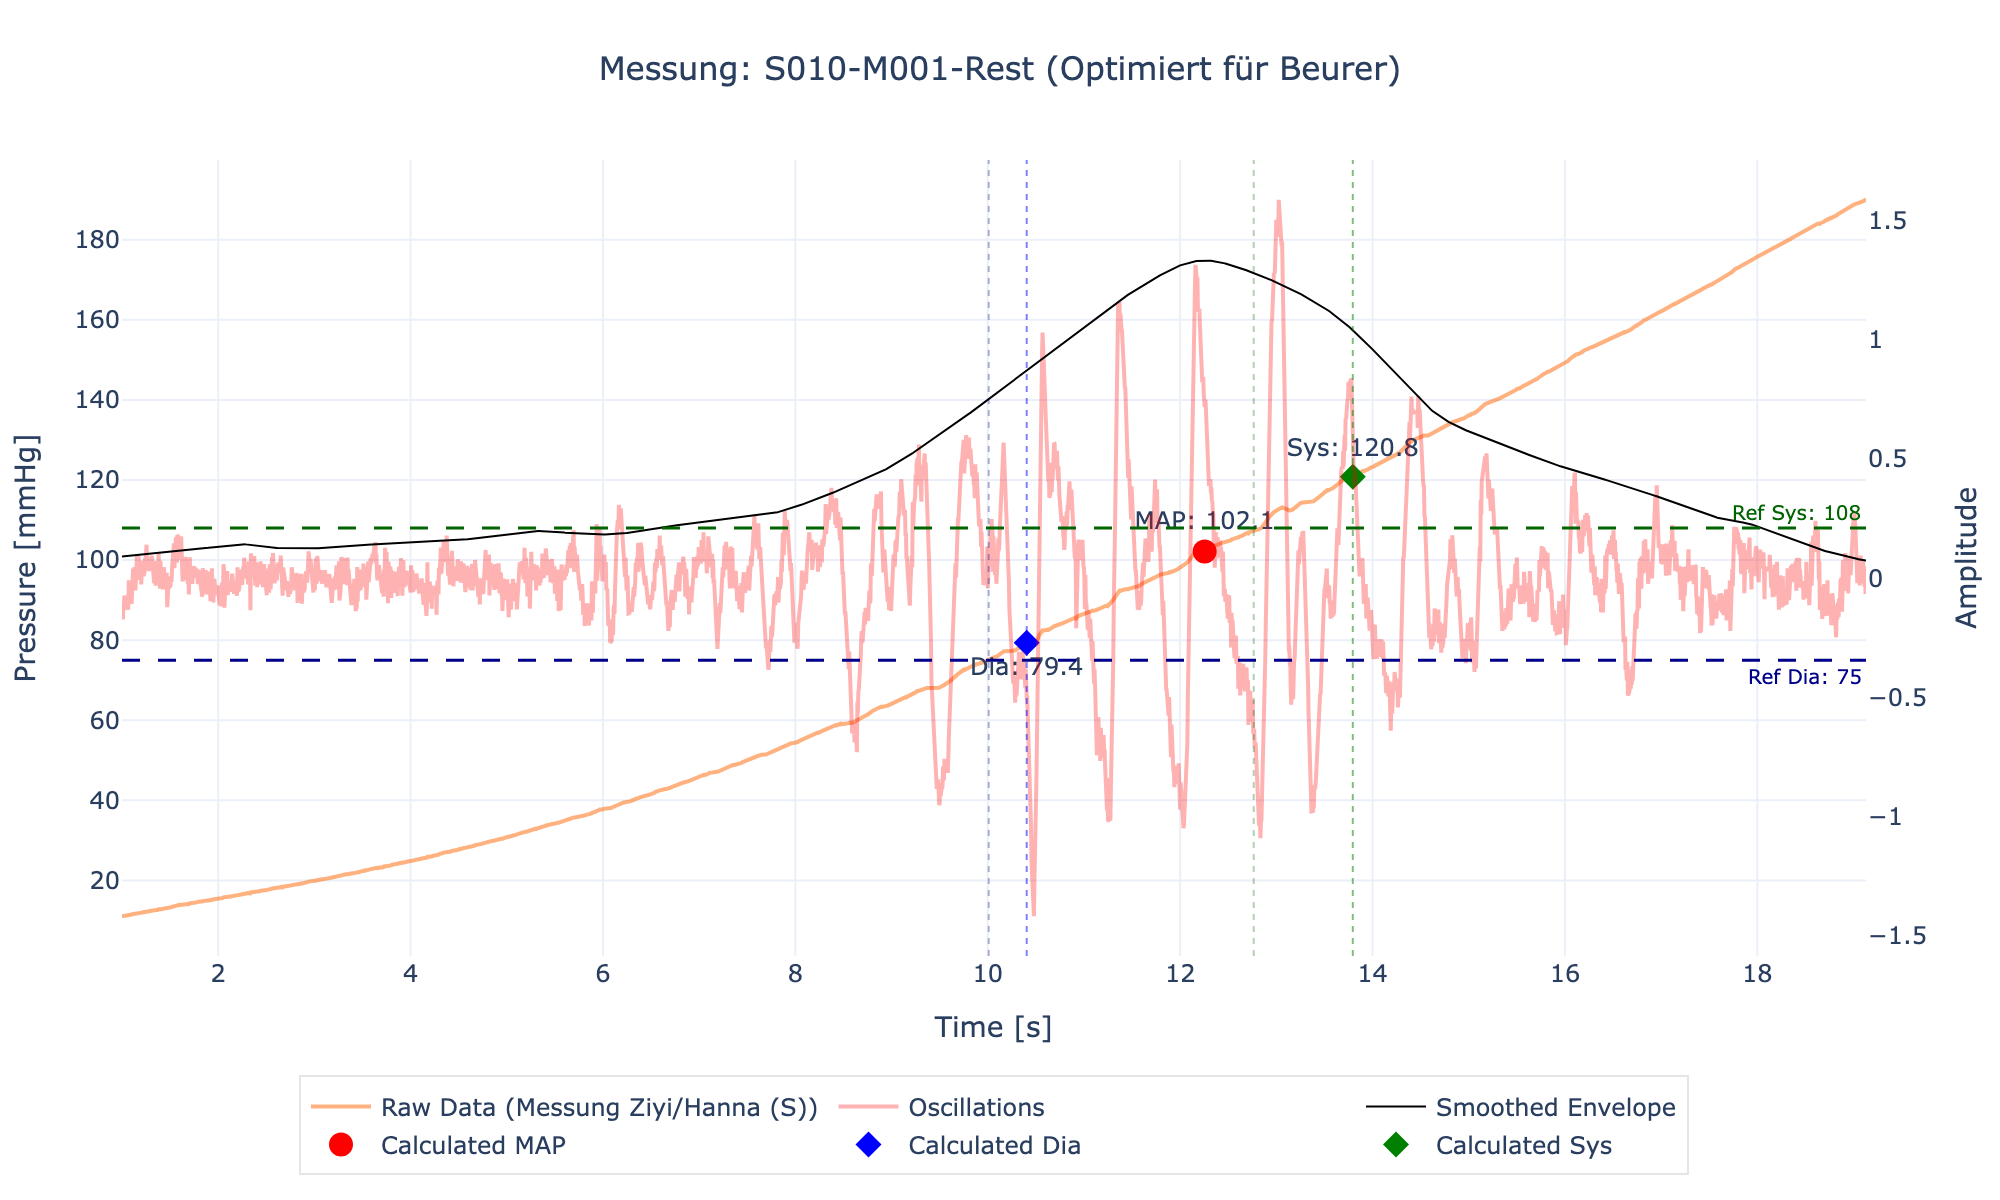
\includegraphics[width=\textwidth]{images/S010-M001-Rest_beurer.png}
        \caption{Optimiert für Beurer}
    \end{subfigure}
    \hfill
    \begin{subfigure}[b]{0.48\textwidth}
        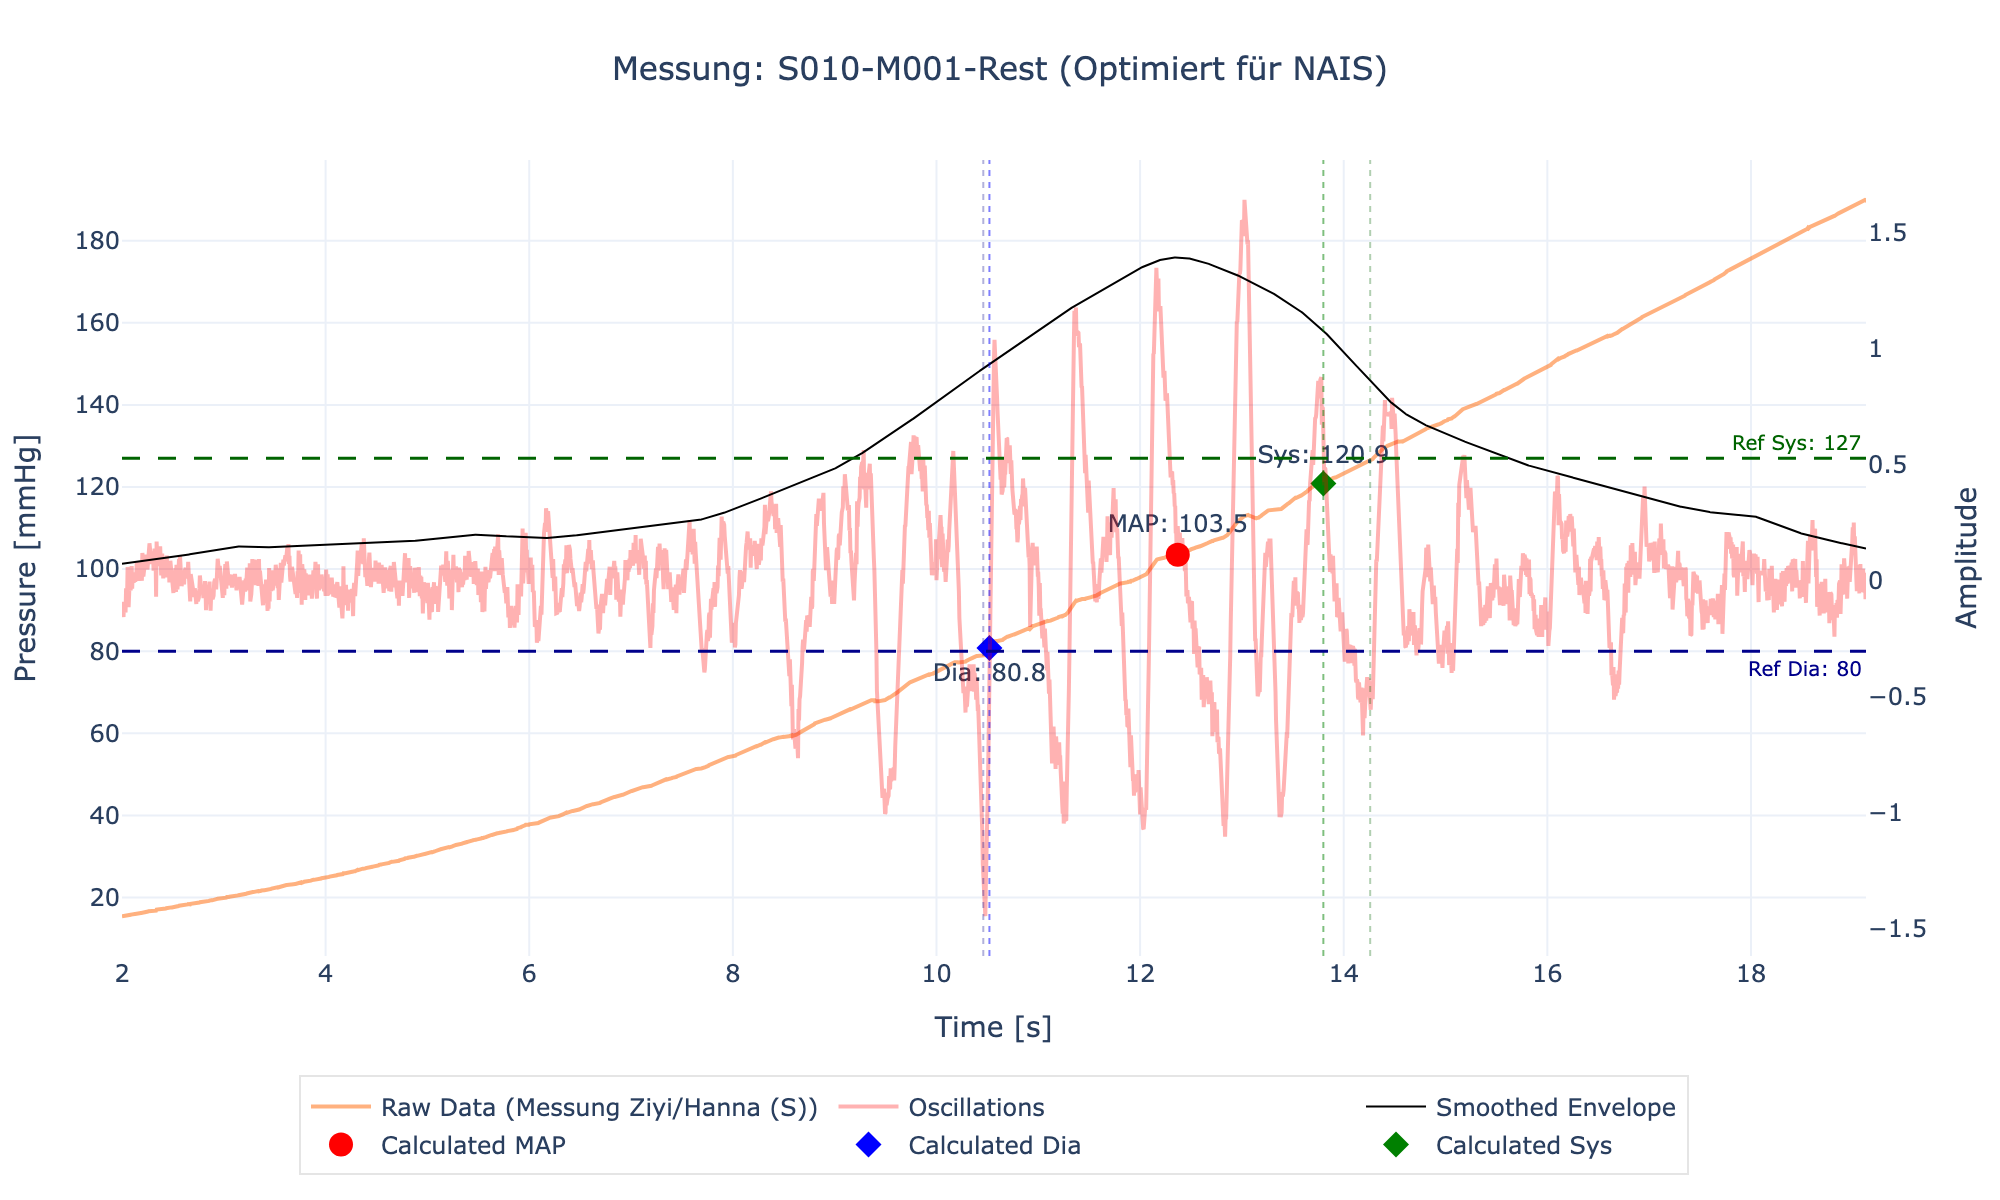
\includegraphics[width=\textwidth]{images/S010-M001-Rest_nais.png}
        \caption{Optimiert für NAIS}
    \end{subfigure}
    \caption{Einzelauswertung der Messung S010-M001-Rest mit verschiedenen Parametersätzen.}
\end{figure}
\newpage

\subsection*{Messung: S010-M002-Active}
\begin{figure}[H]
    \centering
    \begin{subfigure}[b]{0.8\textwidth}
        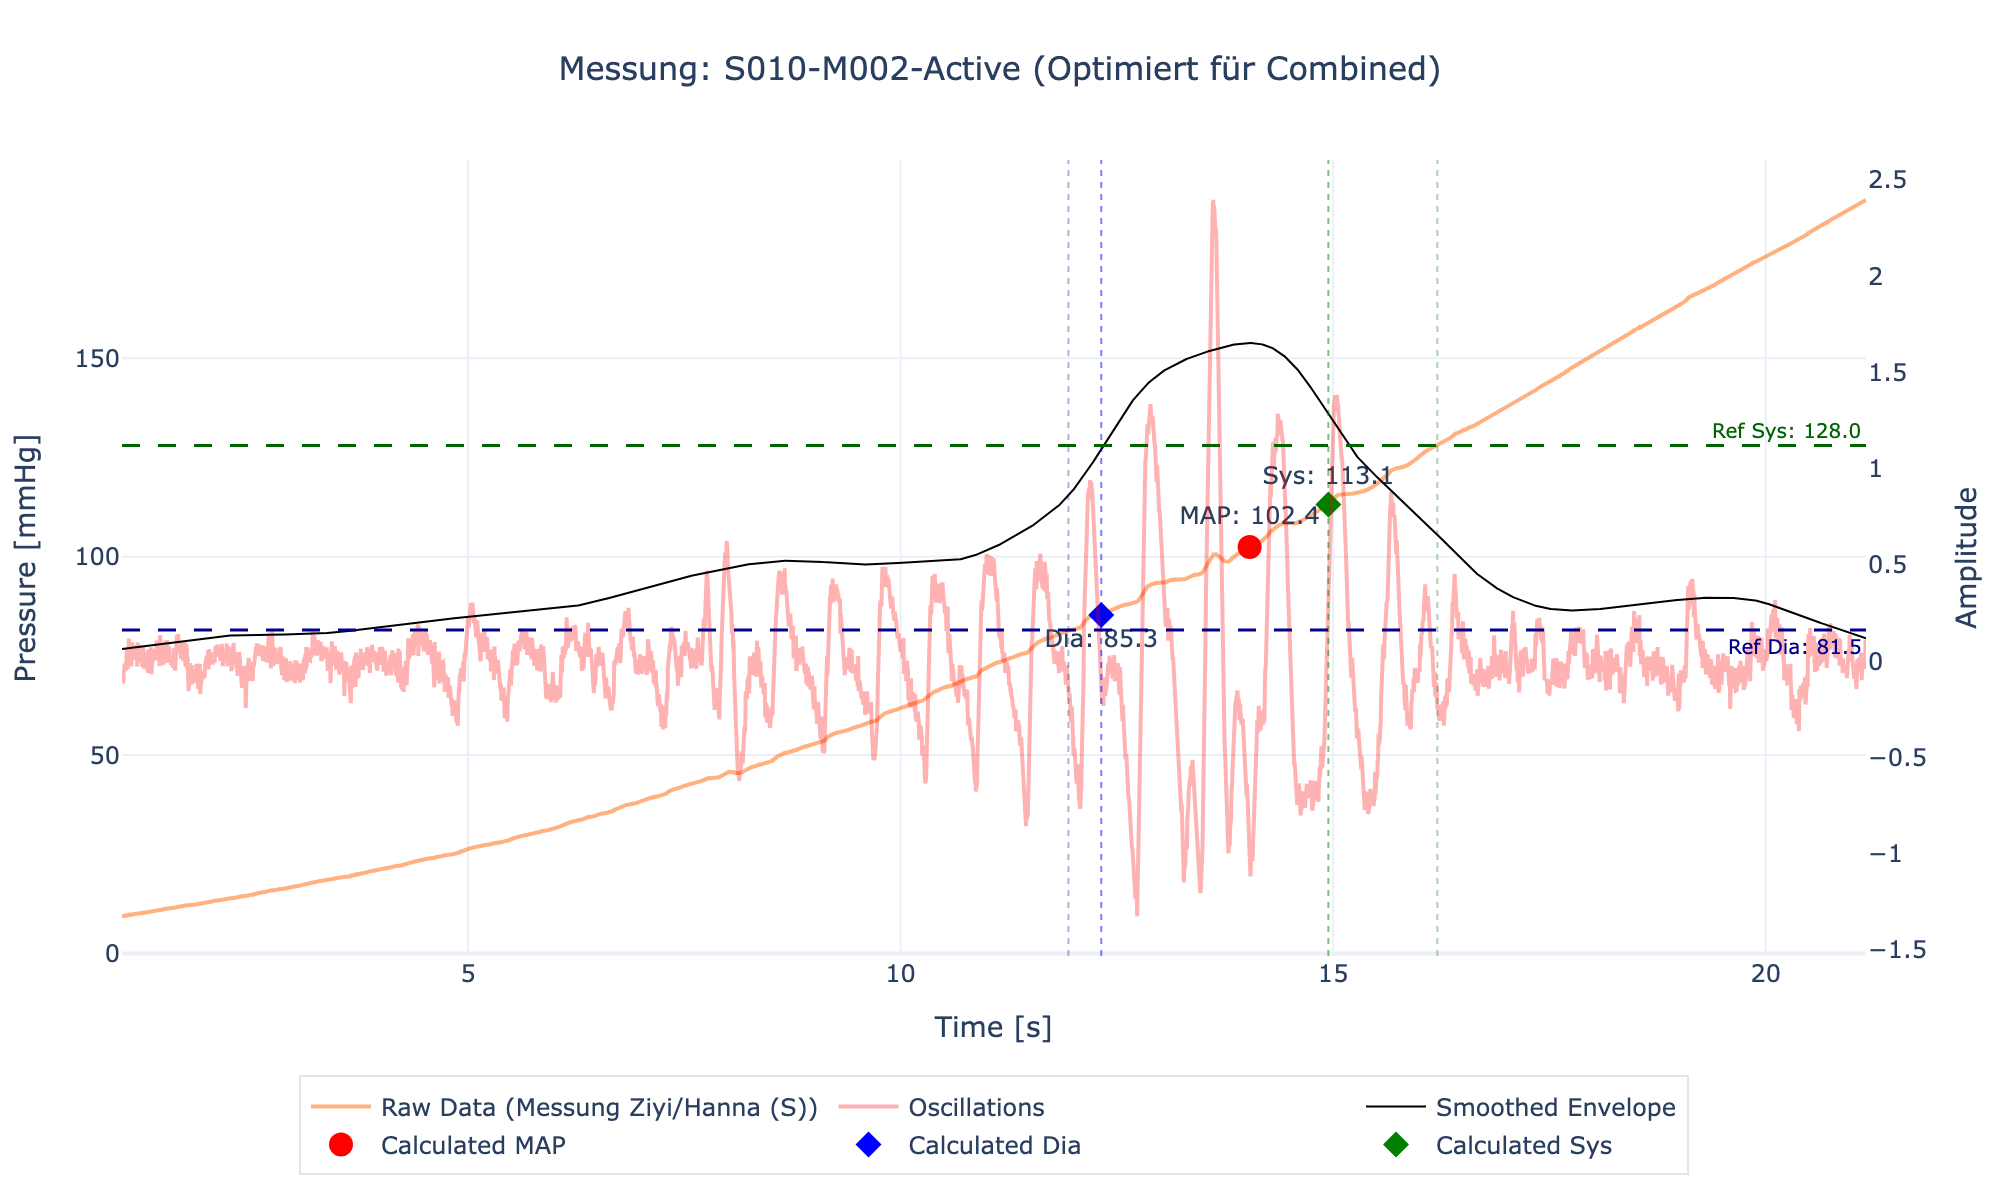
\includegraphics[width=\textwidth]{images/S010-M002-Active_combined.png}
        \caption{Optimiert für Beurer und NAIS (Kombiniert)}
    \end{subfigure} \\
    \begin{subfigure}[b]{0.48\textwidth}
        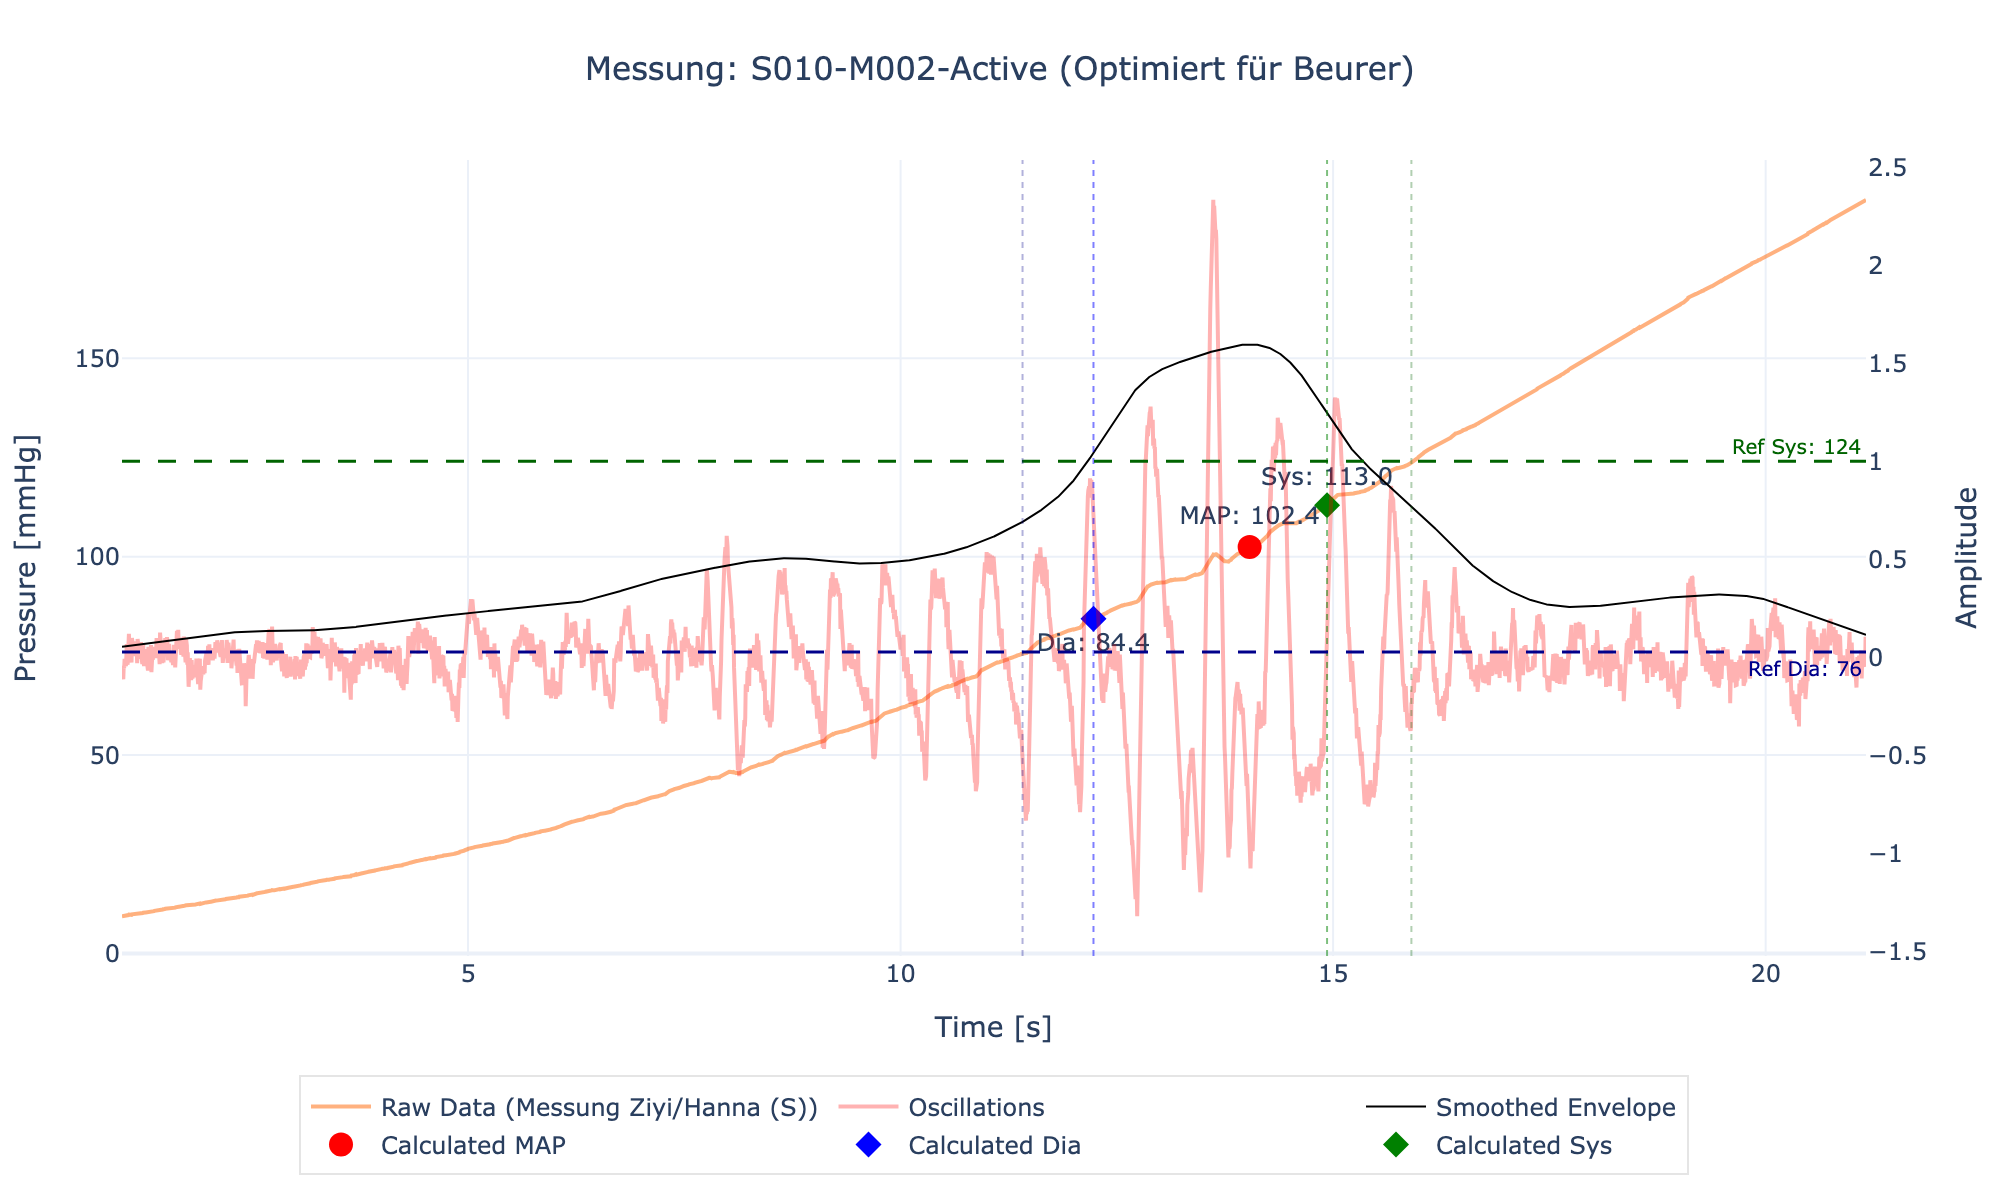
\includegraphics[width=\textwidth]{images/S010-M002-Active_beurer.png}
        \caption{Optimiert für Beurer}
    \end{subfigure}
    \hfill
    \begin{subfigure}[b]{0.48\textwidth}
        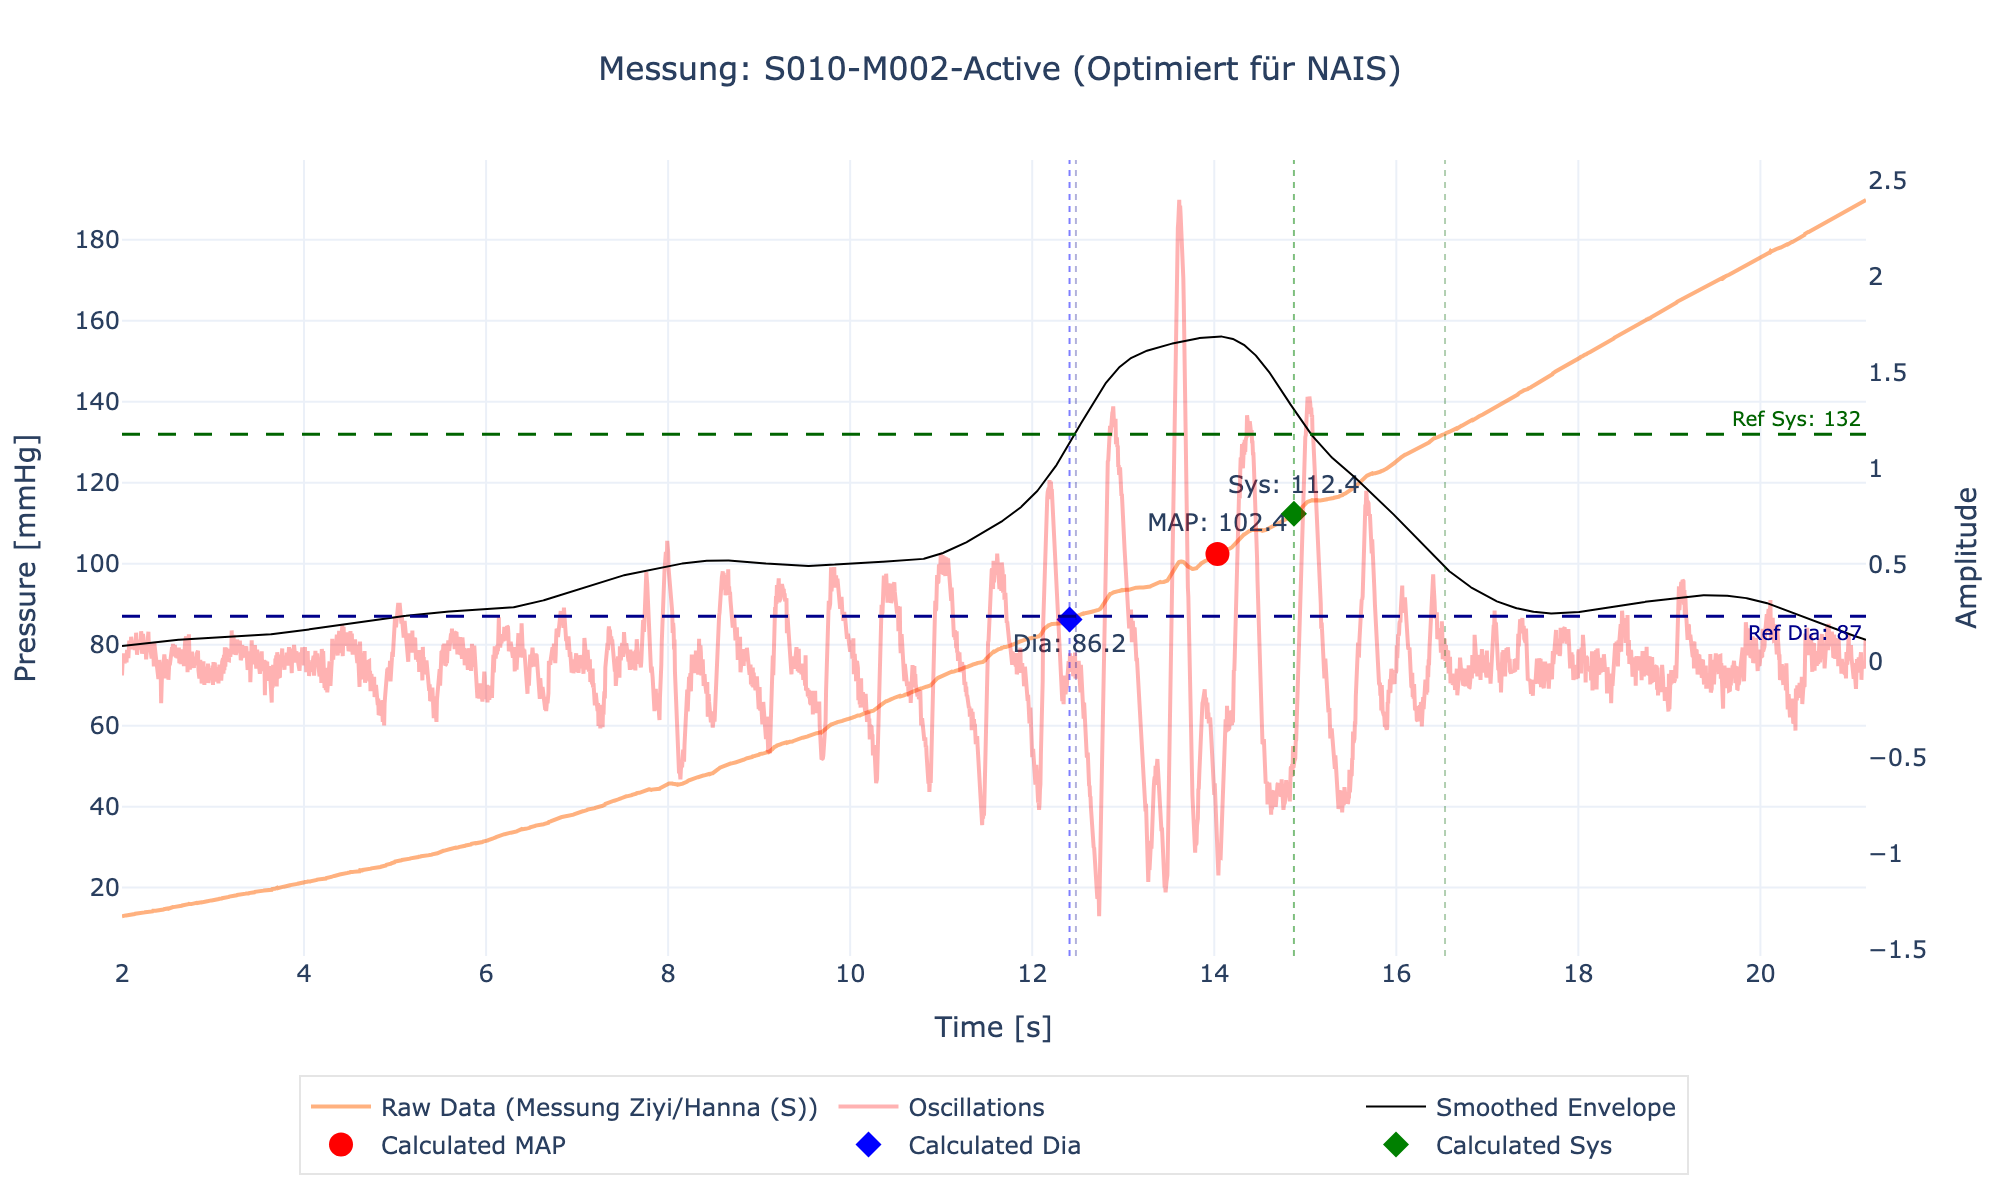
\includegraphics[width=\textwidth]{images/S010-M002-Active_nais.png}
        \caption{Optimiert für NAIS}
    \end{subfigure}
    \caption{Einzelauswertung der Messung S010-M002-Active mit verschiedenen Parametersätzen.}
\end{figure}
\newpage

\subsection*{Messung: S011-M001-Rest}
\begin{figure}[H]
    \centering
    \begin{subfigure}[b]{0.8\textwidth}
        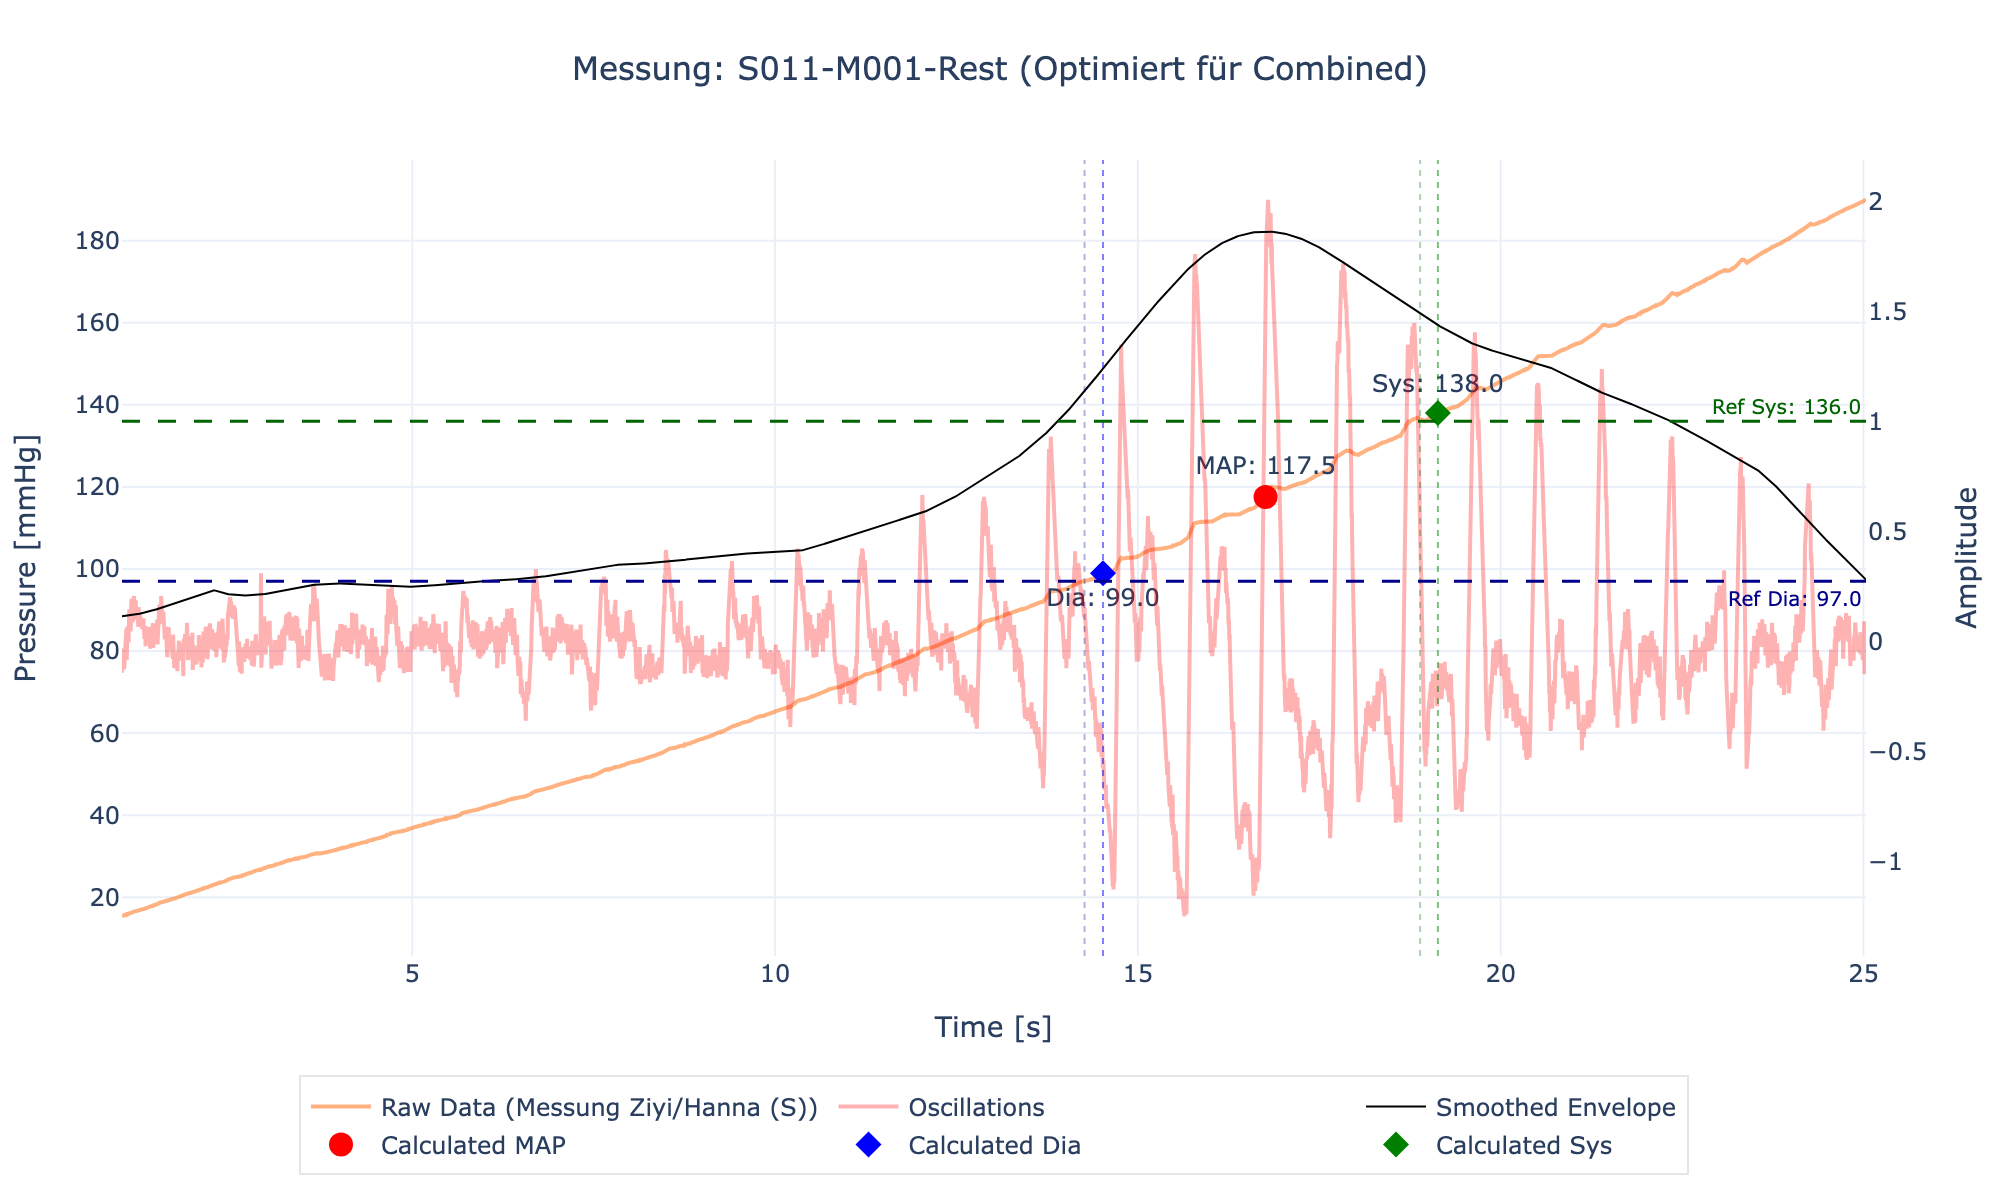
\includegraphics[width=\textwidth]{images/S011-M001-Rest_combined.png}
        \caption{Optimiert für Beurer und NAIS (Kombiniert)}
    \end{subfigure} \\
    \begin{subfigure}[b]{0.48\textwidth}
        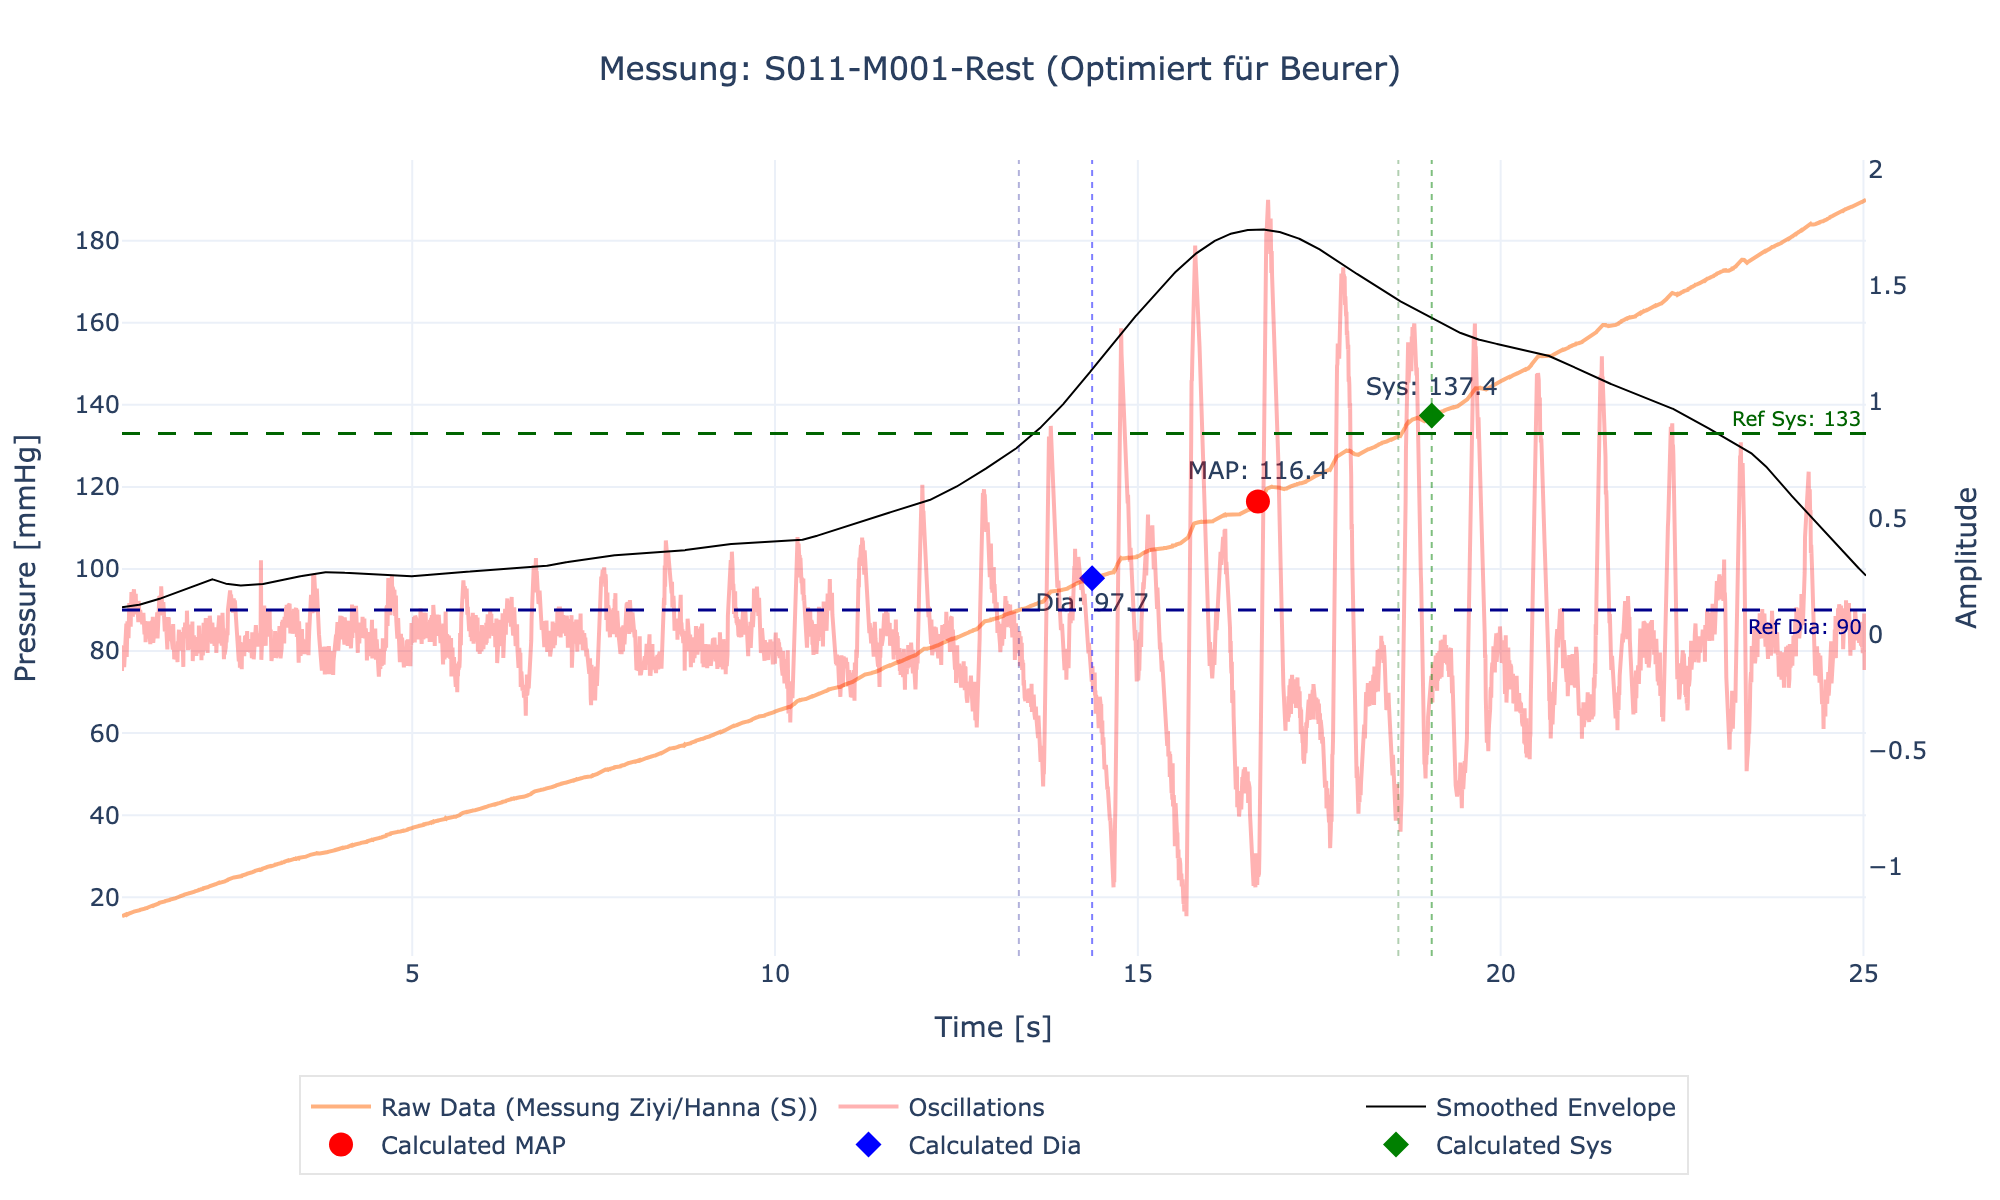
\includegraphics[width=\textwidth]{images/S011-M001-Rest_beurer.png}
        \caption{Optimiert für Beurer}
    \end{subfigure}
    \hfill
    \begin{subfigure}[b]{0.48\textwidth}
        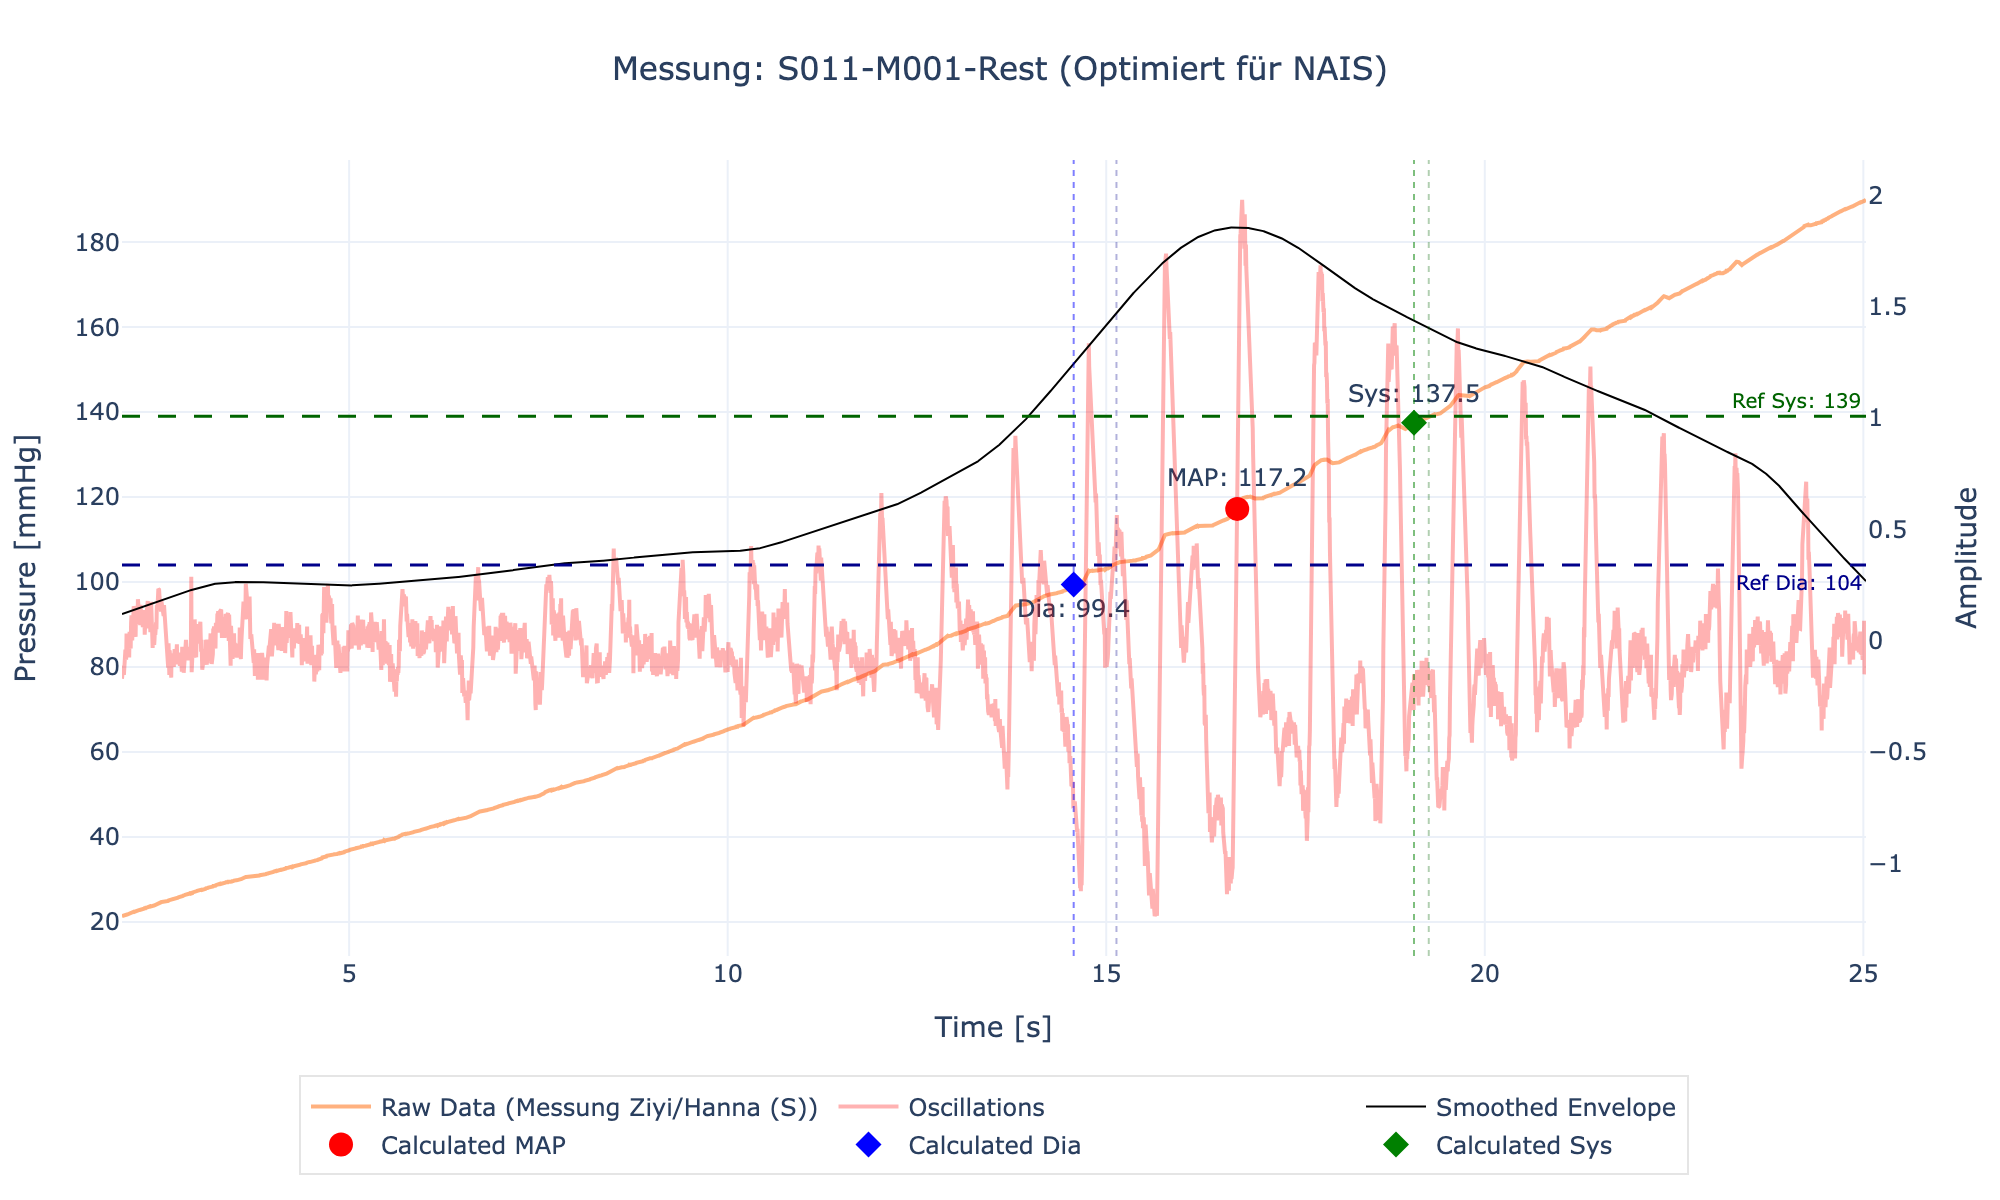
\includegraphics[width=\textwidth]{images/S011-M001-Rest_nais.png}
        \caption{Optimiert für NAIS}
    \end{subfigure}
    \caption{Einzelauswertung der Messung S011-M001-Rest mit verschiedenen Parametersätzen.}
\end{figure}
\newpage

\subsection*{Messung: S011-M002-Active}
\begin{figure}[H]
    \centering
    \begin{subfigure}[b]{0.8\textwidth}
        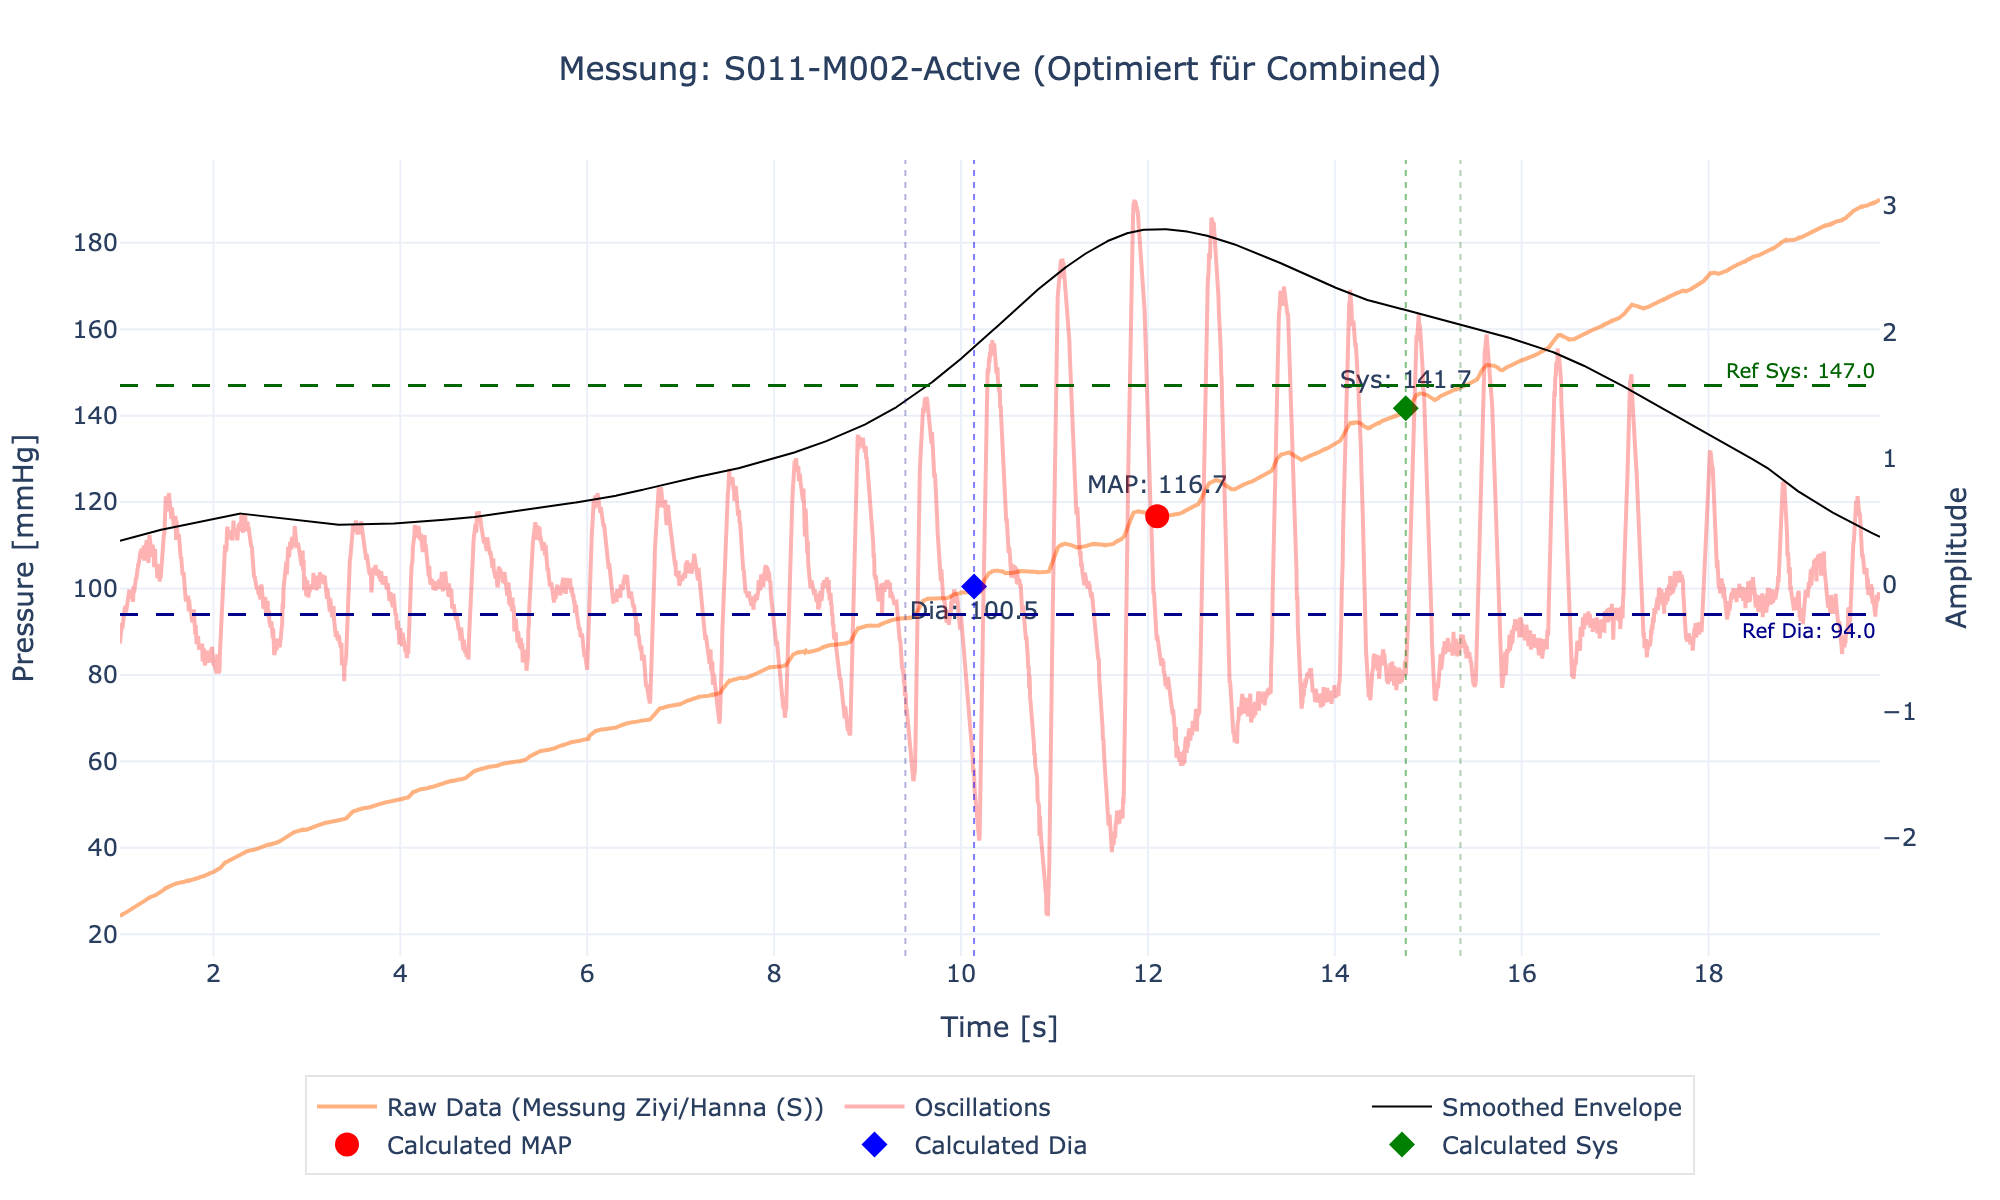
\includegraphics[width=\textwidth]{images/S011-M002-Active_combined.png}
        \caption{Optimiert für Beurer und NAIS (Kombiniert)}
    \end{subfigure} \\
    \begin{subfigure}[b]{0.48\textwidth}
        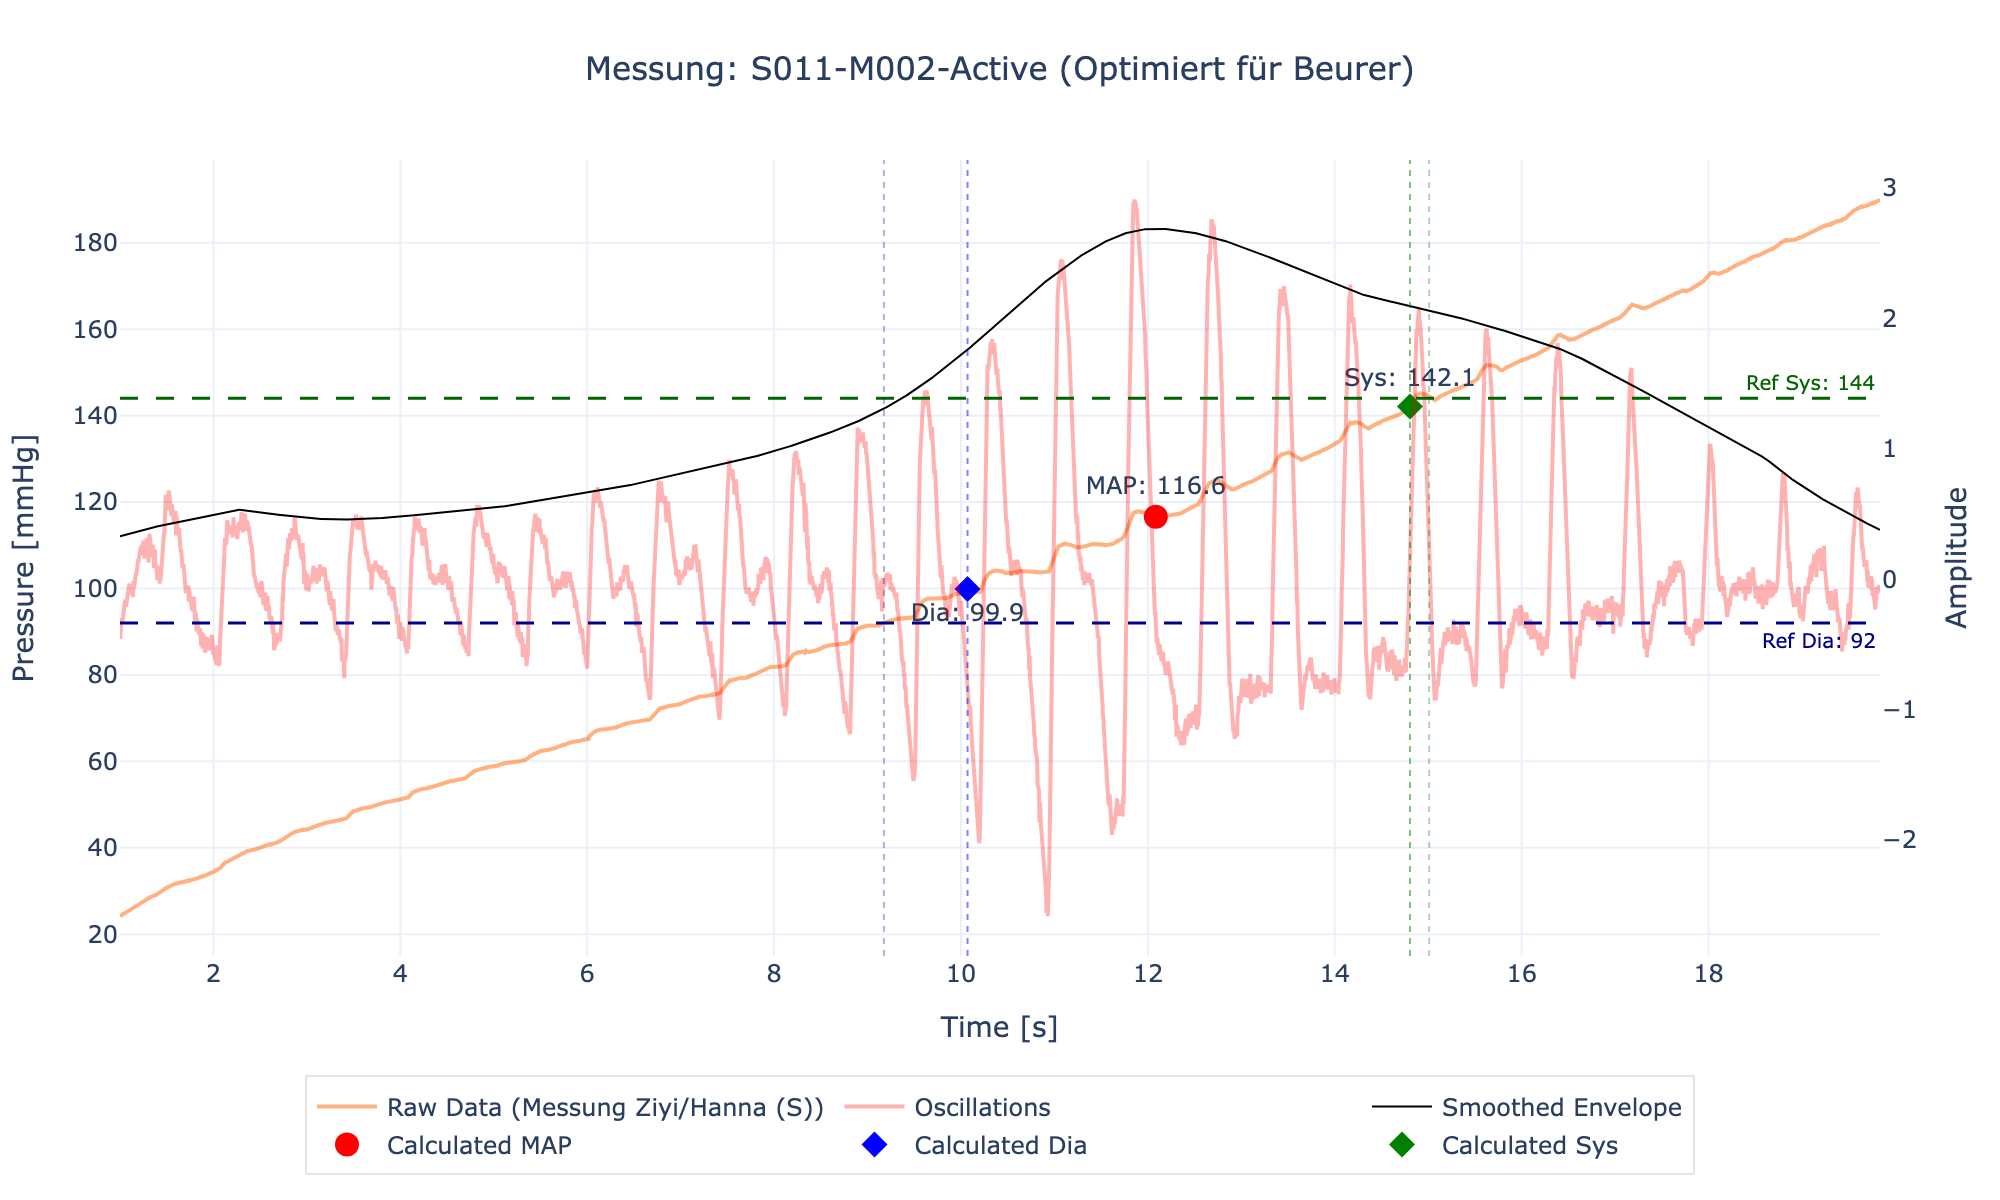
\includegraphics[width=\textwidth]{images/S011-M002-Active_beurer.png}
        \caption{Optimiert für Beurer}
    \end{subfigure}
    \hfill
    \begin{subfigure}[b]{0.48\textwidth}
        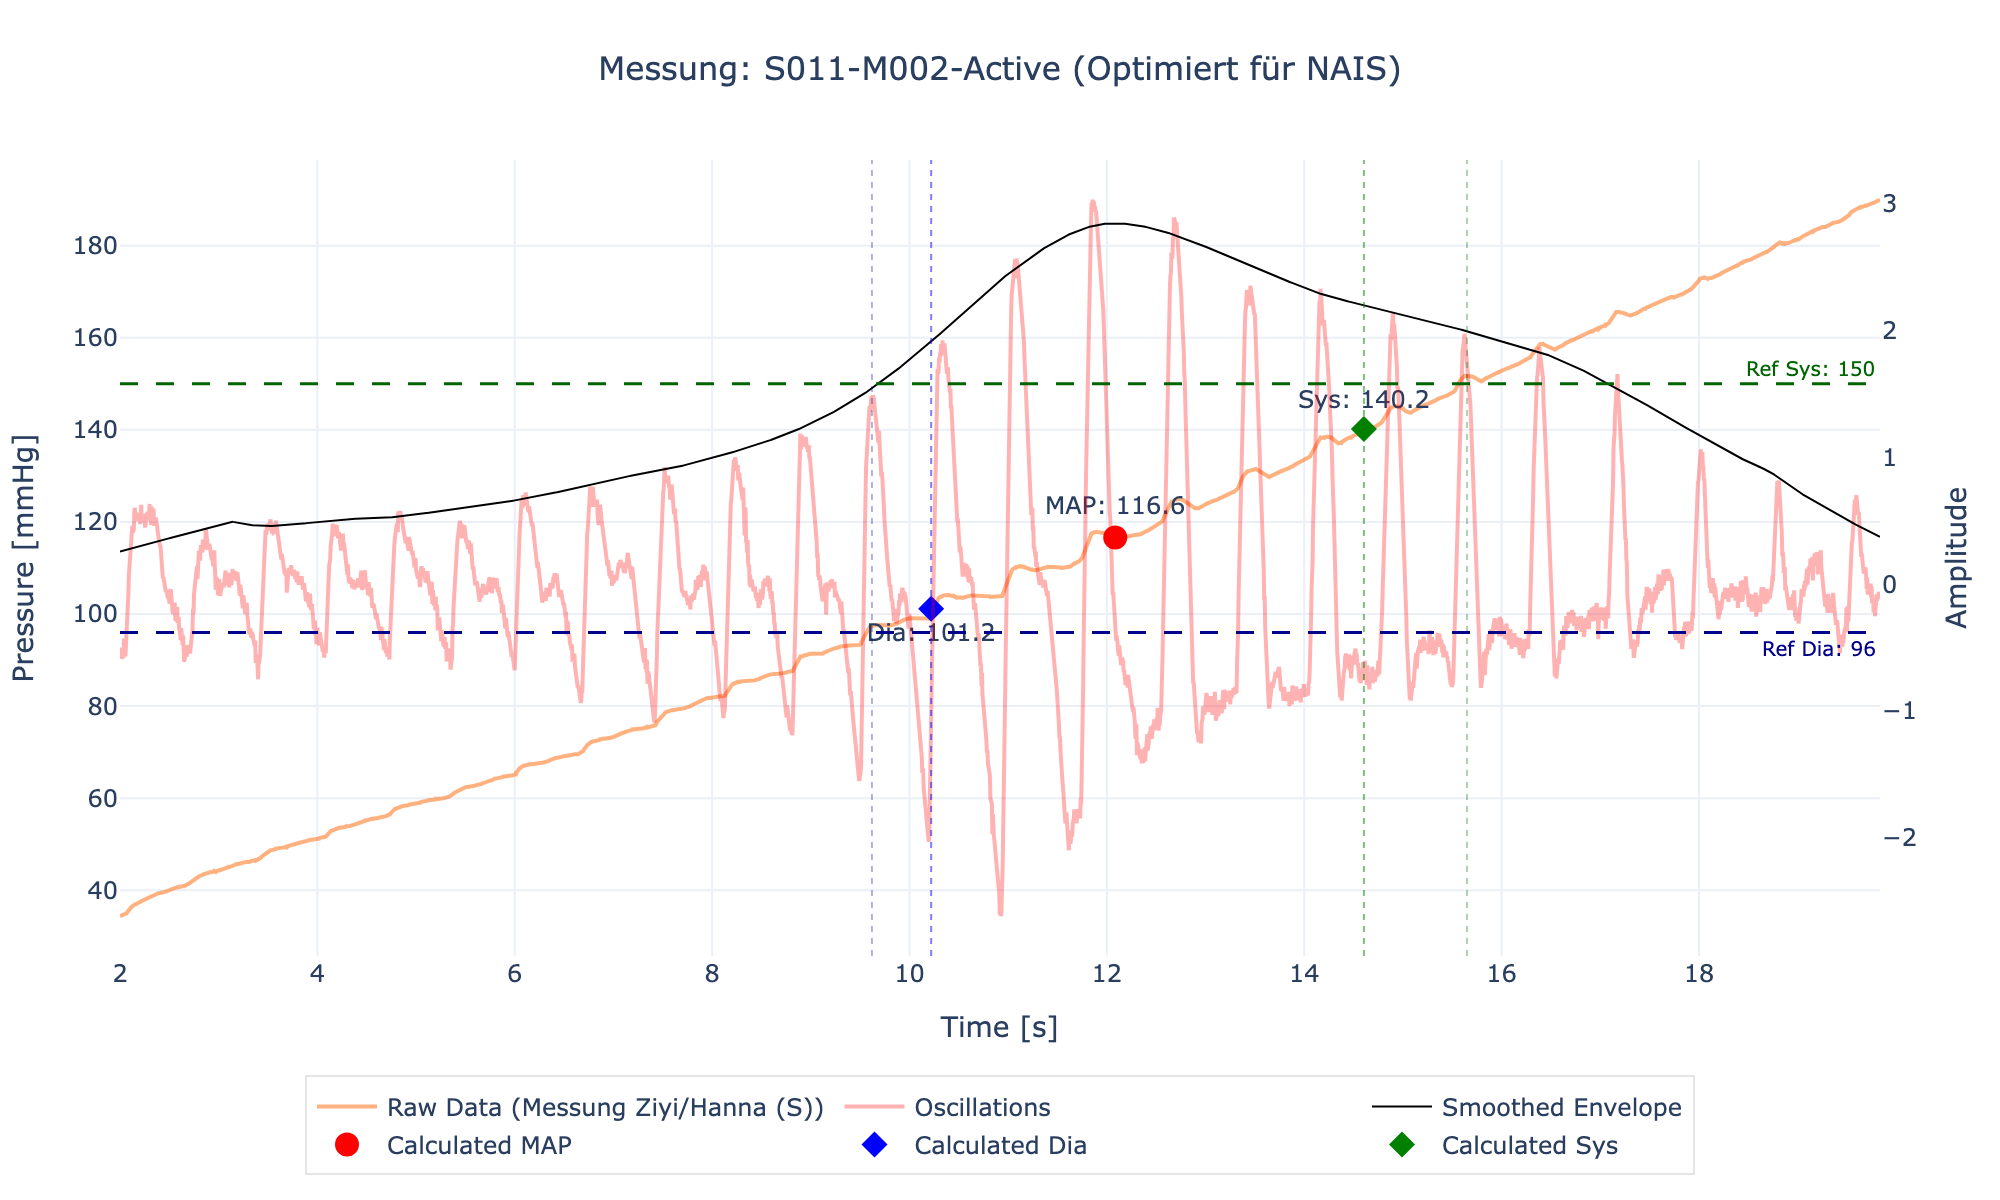
\includegraphics[width=\textwidth]{images/S011-M002-Active_nais.png}
        \caption{Optimiert für NAIS}
    \end{subfigure}
    \caption{Einzelauswertung der Messung S011-M002-Active mit verschiedenen Parametersätzen.}
\end{figure}
\newpage

\subsection*{Messung: S012-M001-Rest}
\begin{figure}[H]
    \centering
    \begin{subfigure}[b]{0.8\textwidth}
        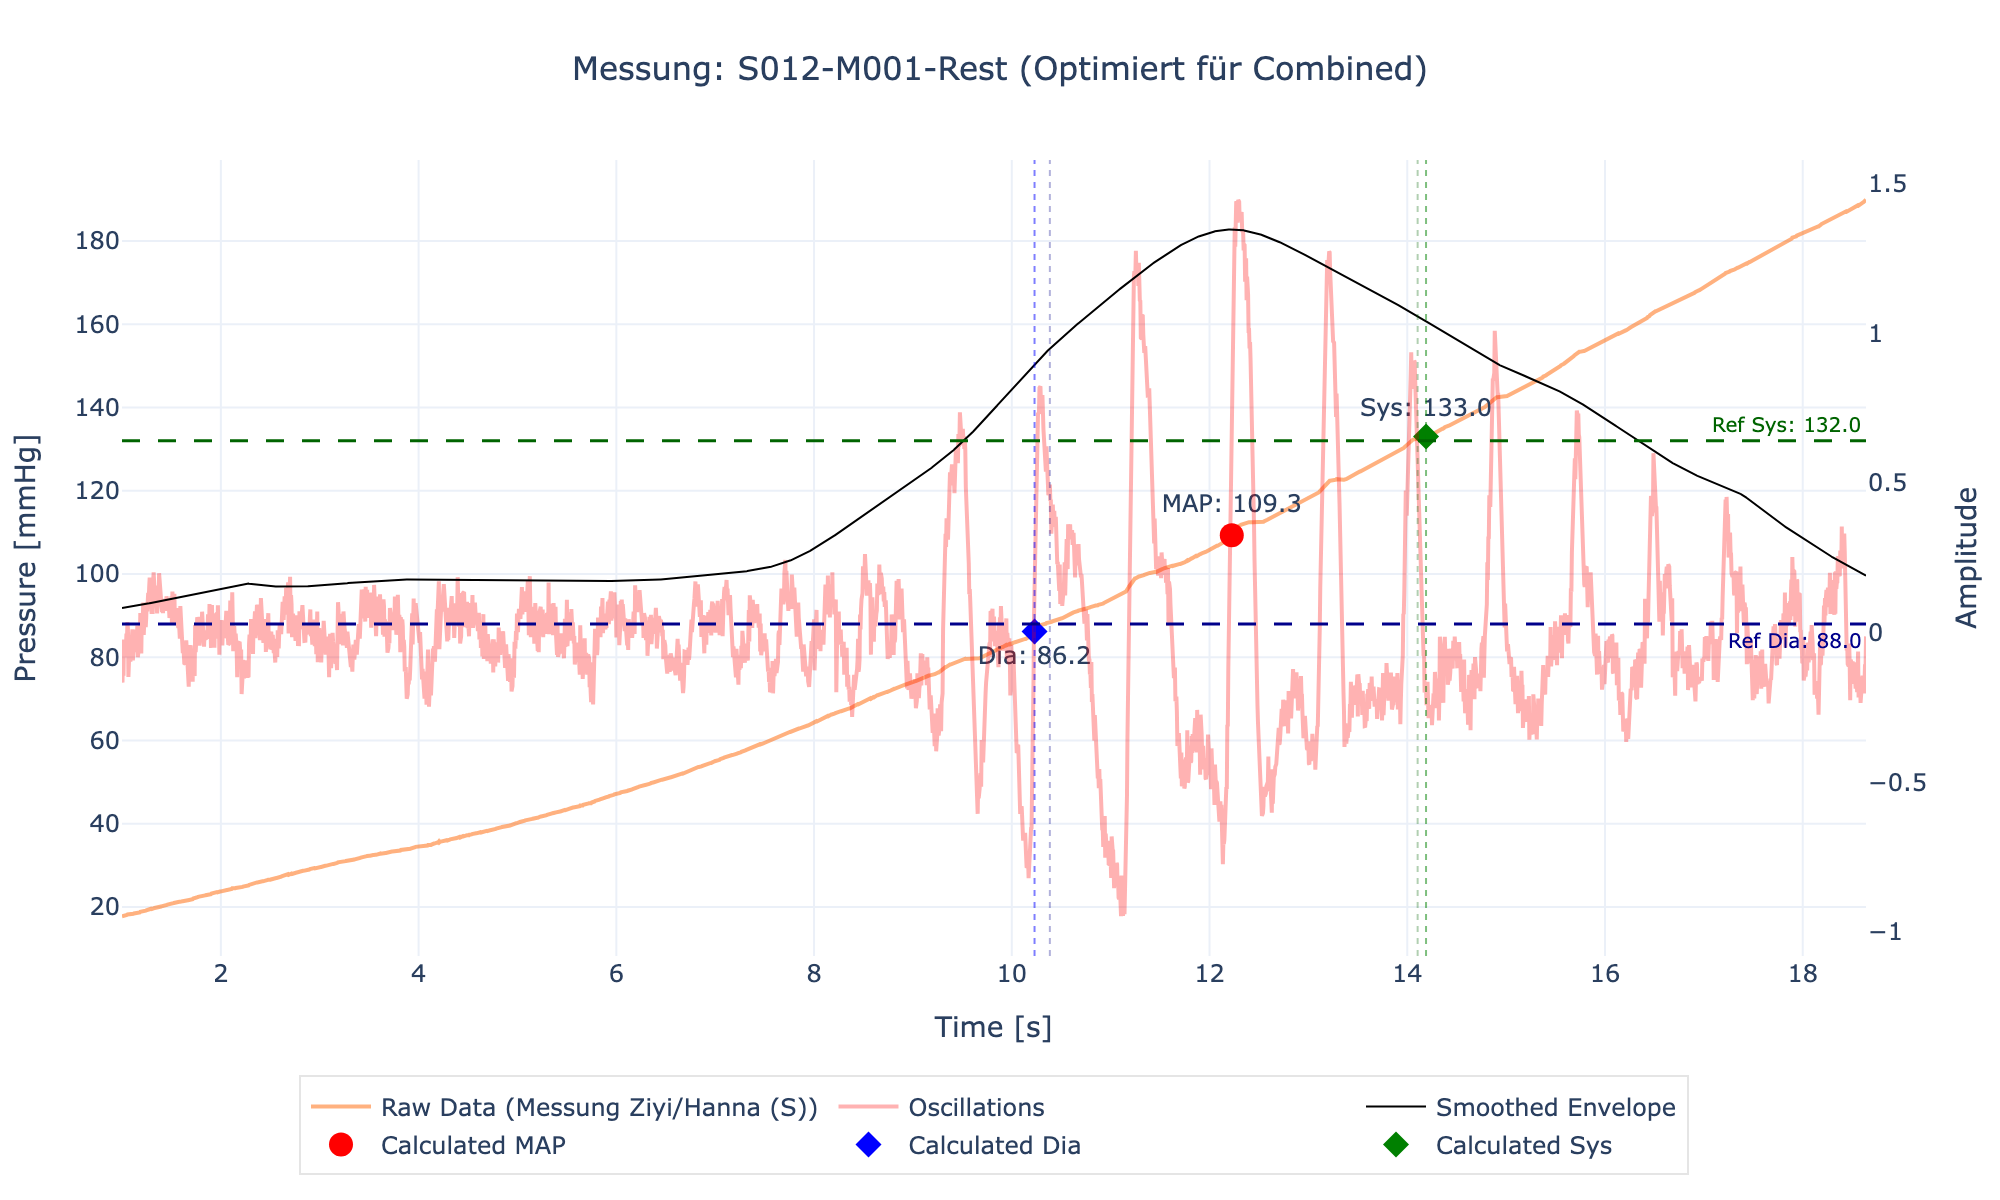
\includegraphics[width=\textwidth]{images/S012-M001-Rest_combined.png}
        \caption{Optimiert für Beurer und NAIS (Kombiniert)}
    \end{subfigure} \\
    \begin{subfigure}[b]{0.48\textwidth}
        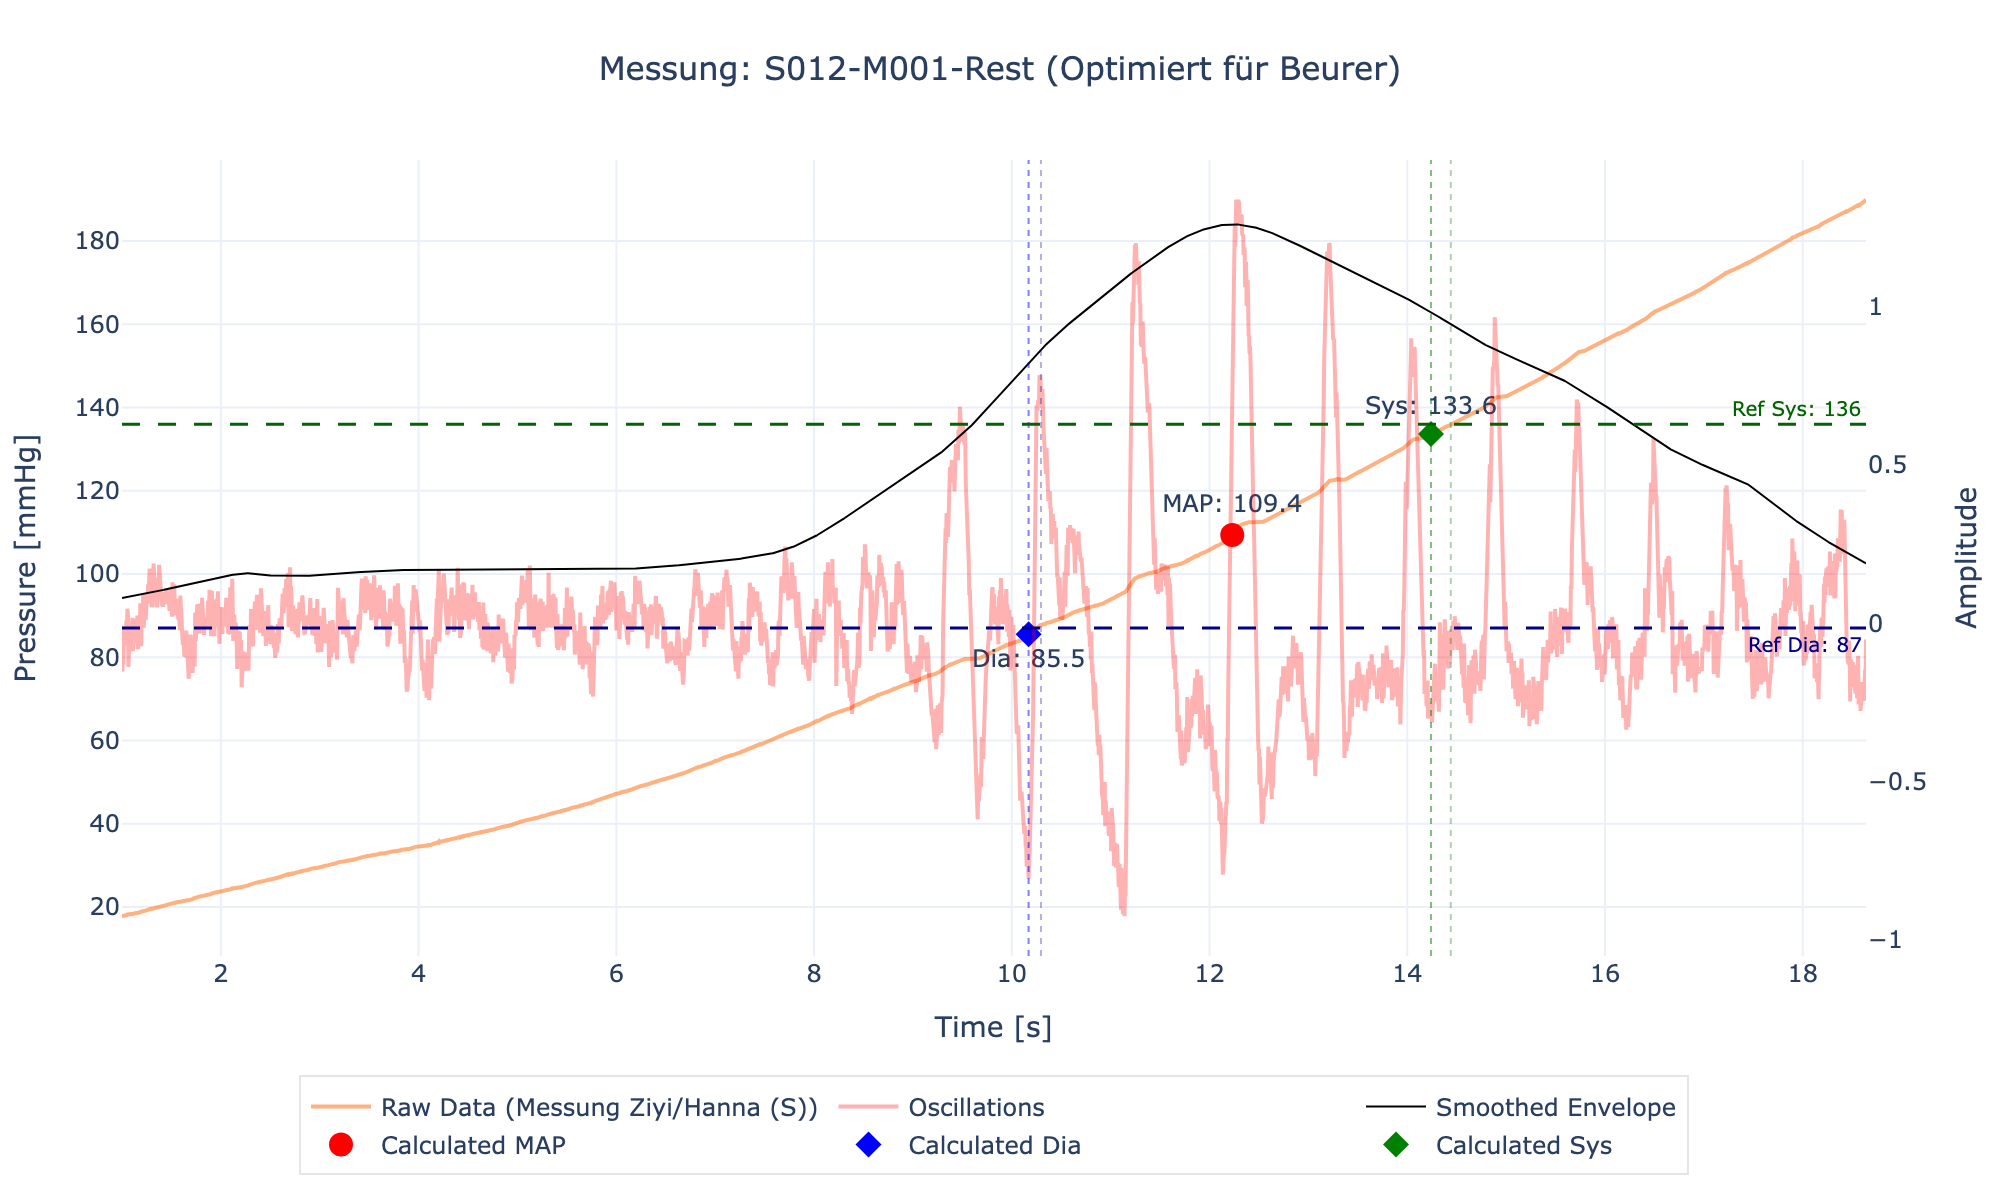
\includegraphics[width=\textwidth]{images/S012-M001-Rest_beurer.png}
        \caption{Optimiert für Beurer}
    \end{subfigure}
    \hfill
    \begin{subfigure}[b]{0.48\textwidth}
        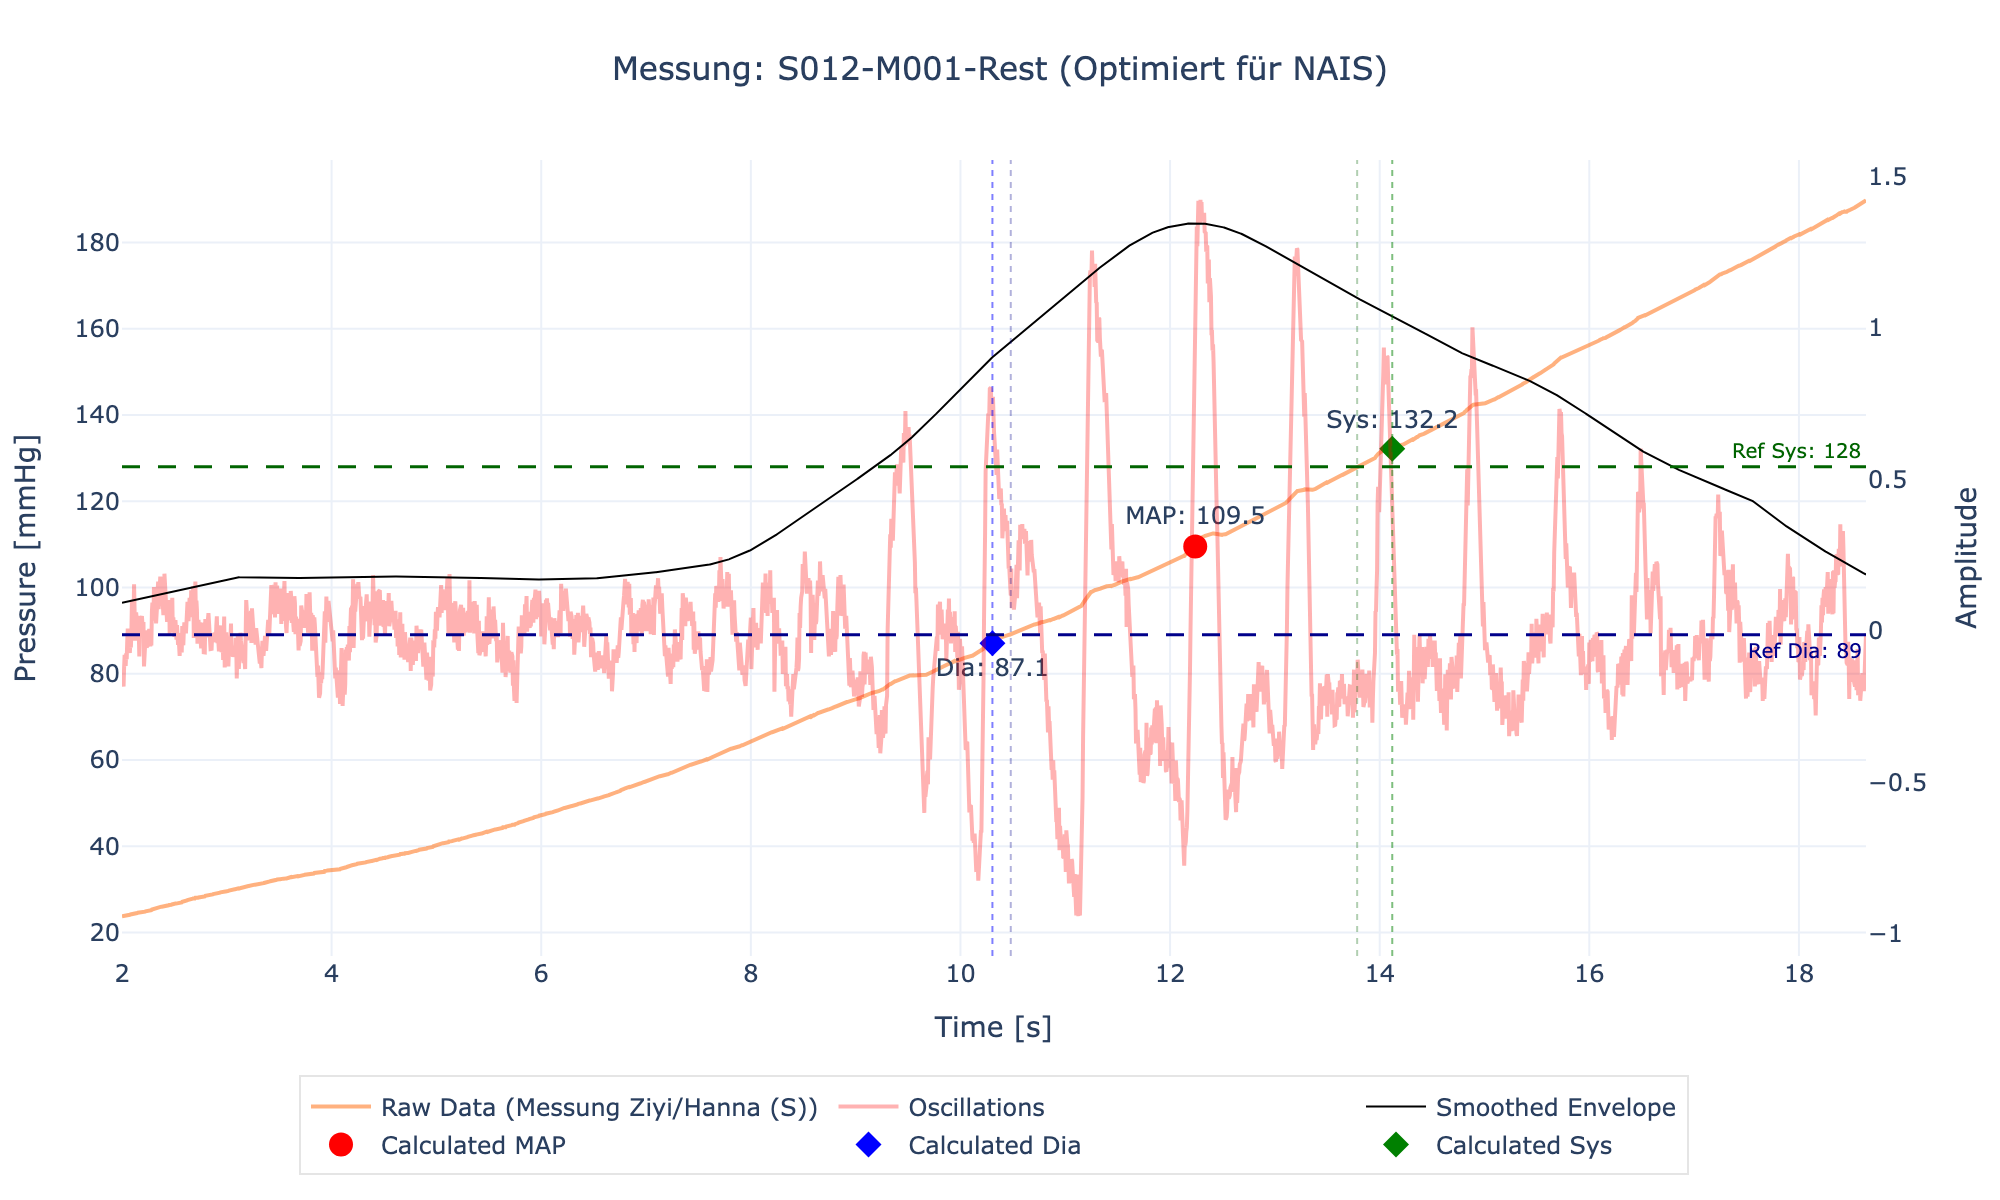
\includegraphics[width=\textwidth]{images/S012-M001-Rest_nais.png}
        \caption{Optimiert für NAIS}
    \end{subfigure}
    \caption{Einzelauswertung der Messung S012-M001-Rest mit verschiedenen Parametersätzen.}
\end{figure}
\newpage

\subsection*{Messung: S012-M002-Active}
\begin{figure}[H]
    \centering
    \begin{subfigure}[b]{0.8\textwidth}
        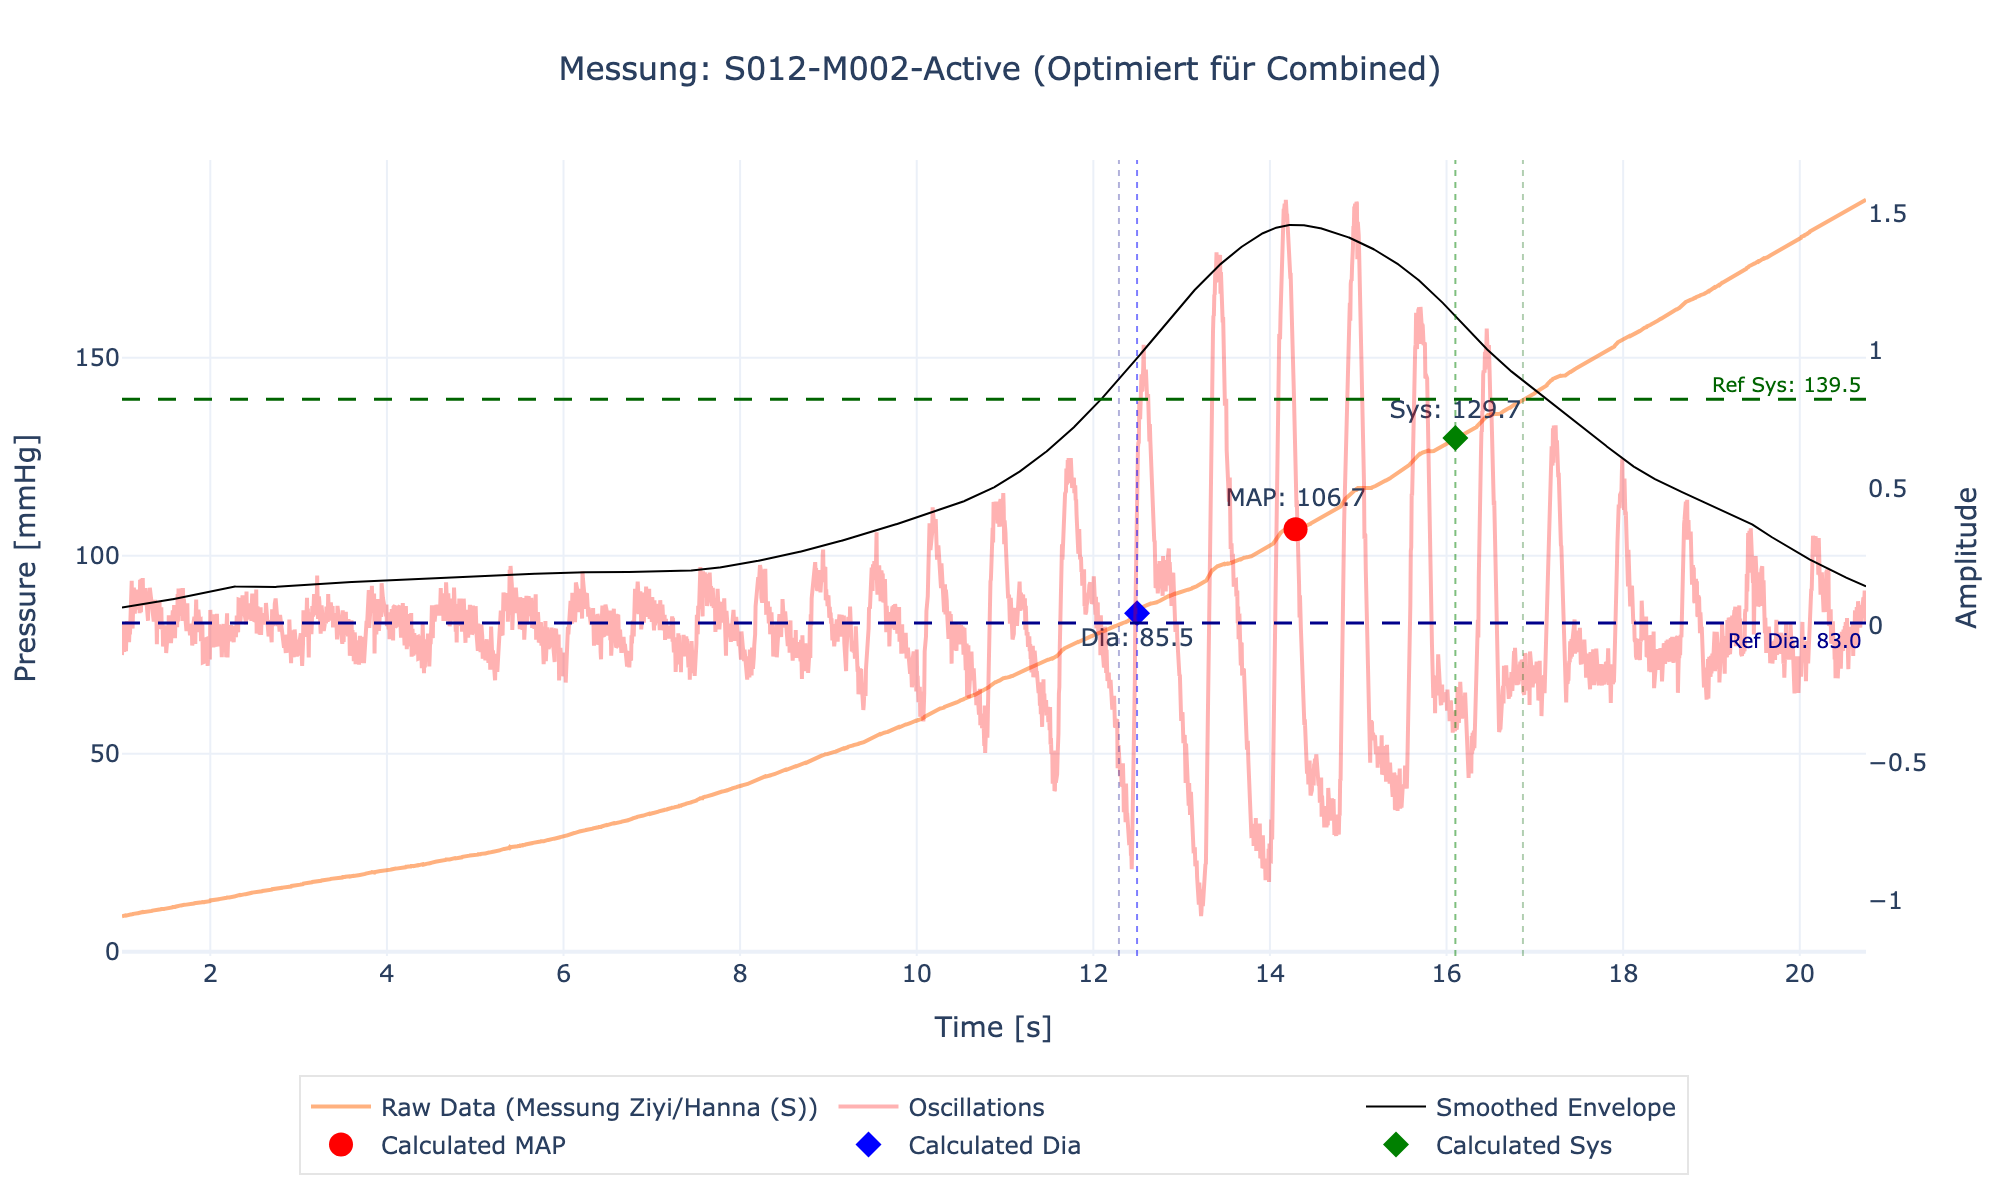
\includegraphics[width=\textwidth]{images/S012-M002-Active_combined.png}
        \caption{Optimiert für Beurer und NAIS (Kombiniert)}
    \end{subfigure} \\
    \begin{subfigure}[b]{0.48\textwidth}
        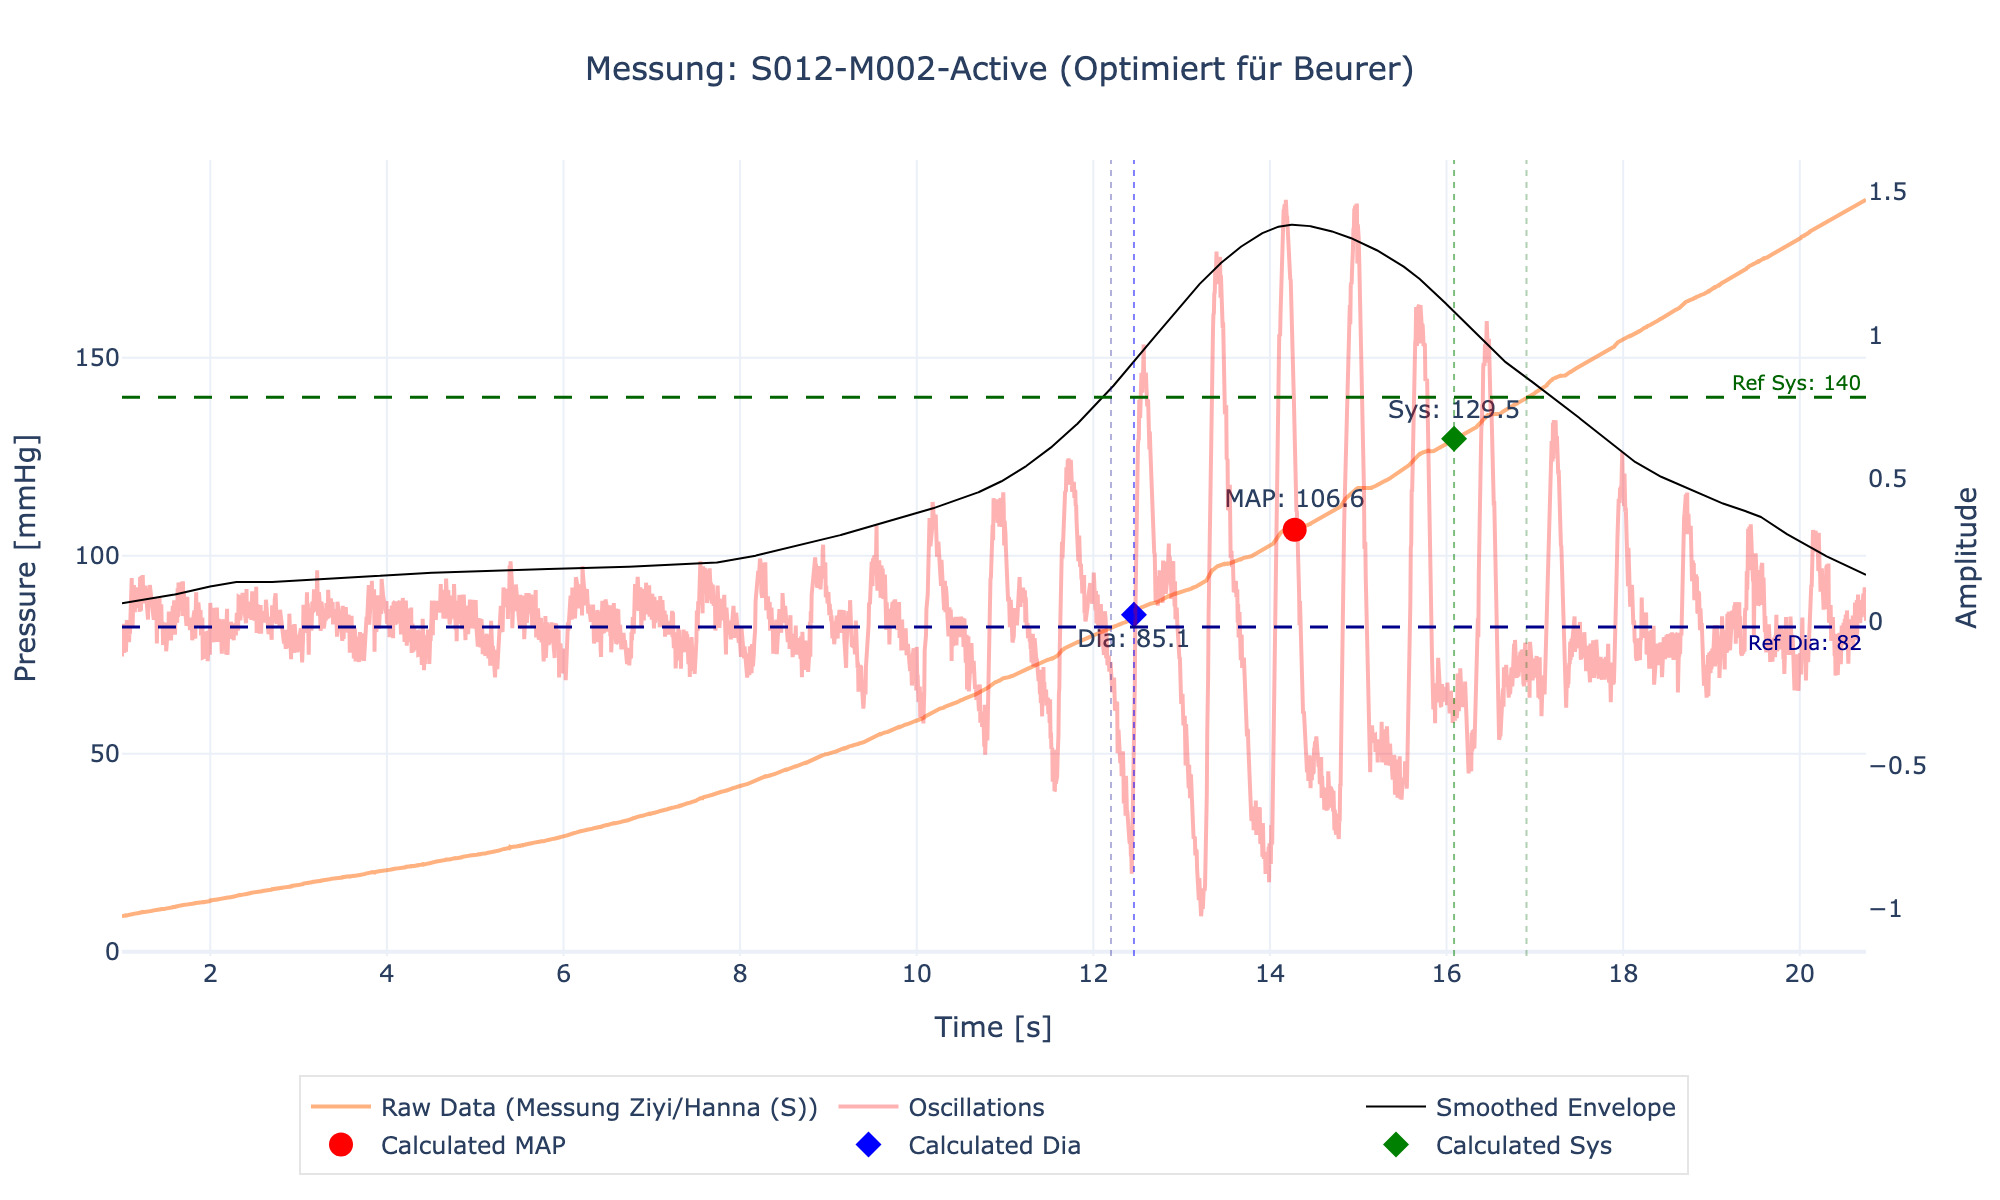
\includegraphics[width=\textwidth]{images/S012-M002-Active_beurer.png}
        \caption{Optimiert für Beurer}
    \end{subfigure}
    \hfill
    \begin{subfigure}[b]{0.48\textwidth}
        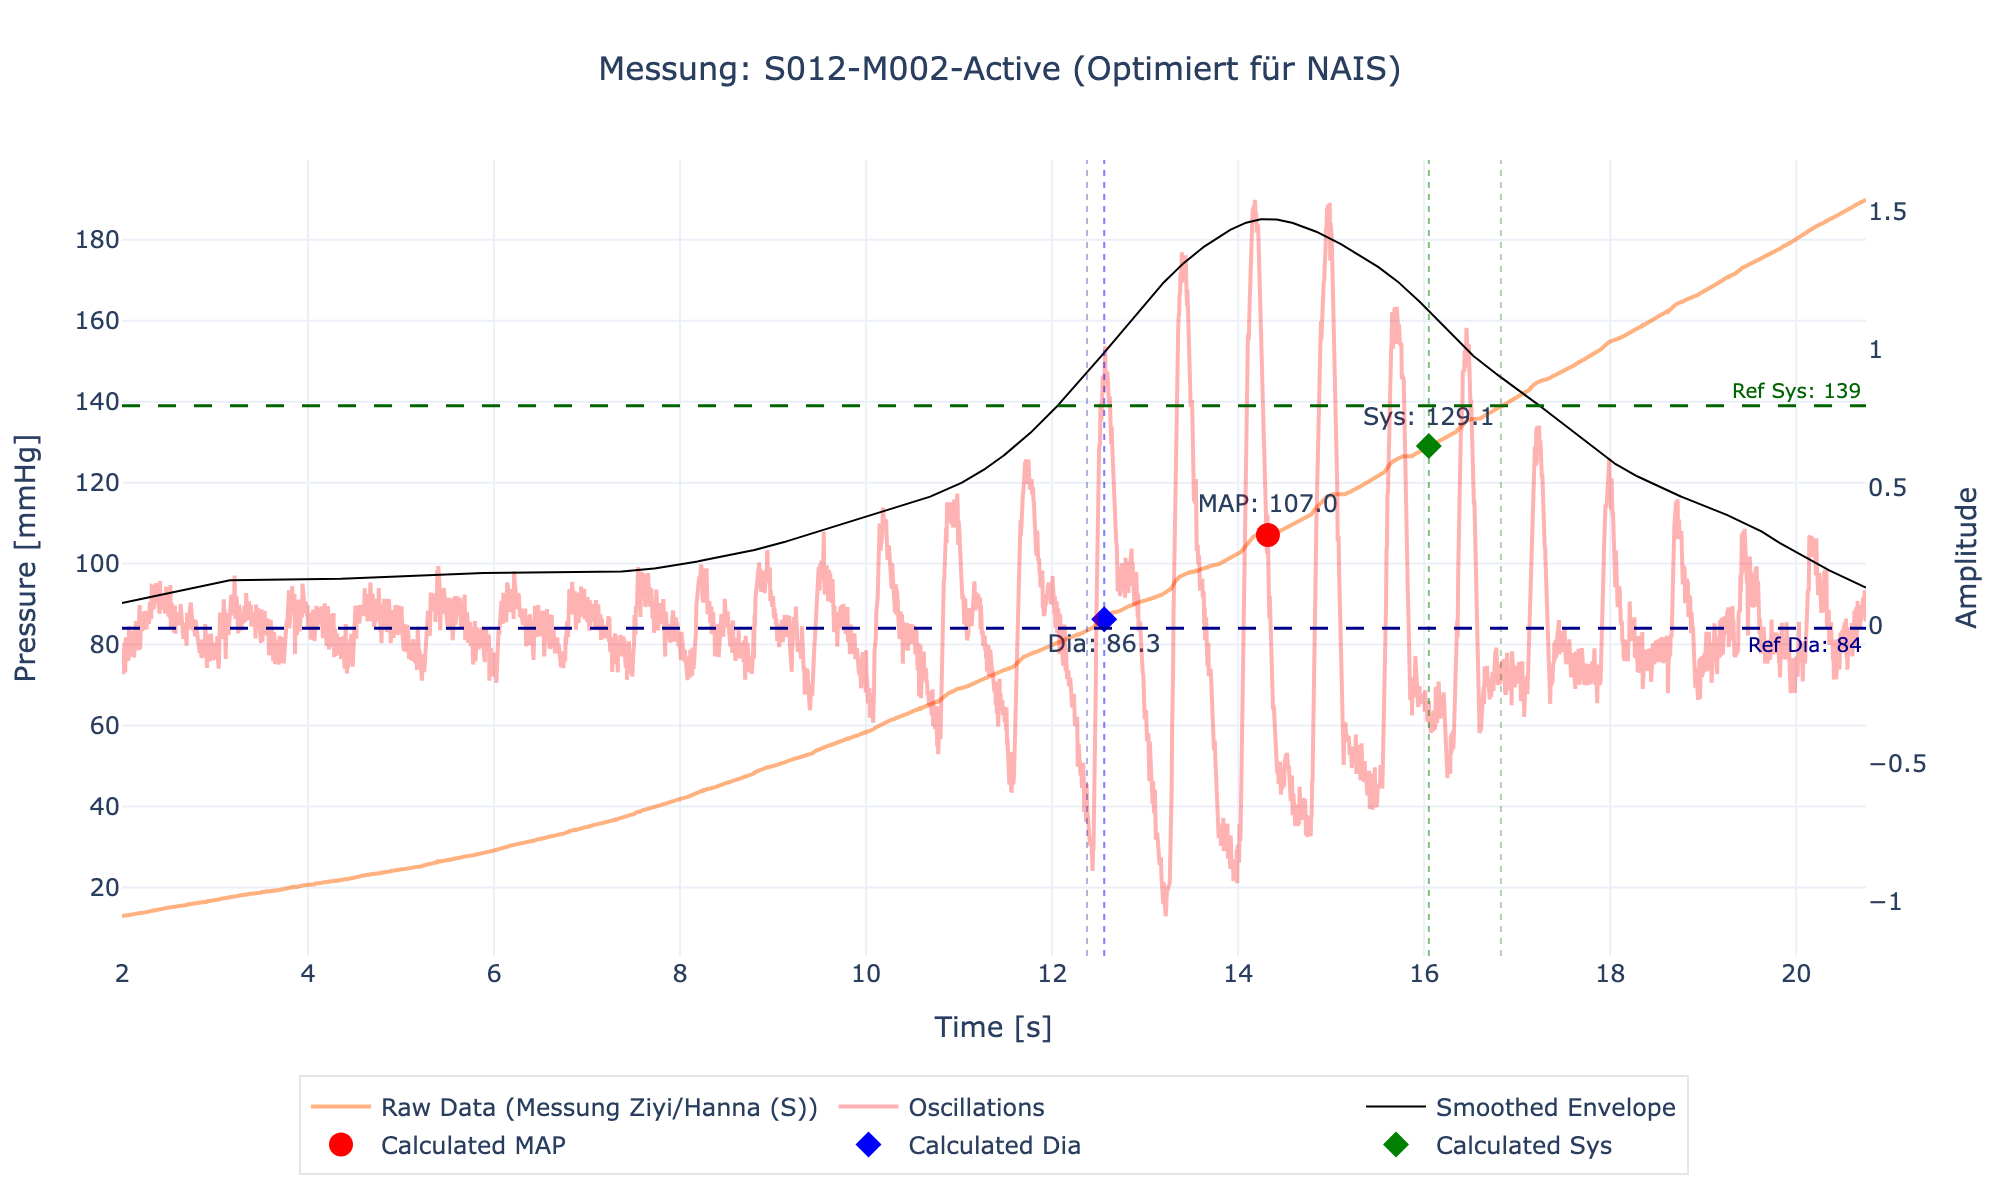
\includegraphics[width=\textwidth]{images/S012-M002-Active_nais.png}
        \caption{Optimiert für NAIS}
    \end{subfigure}
    \caption{Einzelauswertung der Messung S012-M002-Active mit verschiedenen Parametersätzen.}
\end{figure}
\newpage

\subsection*{Messung: S013-M001-Rest}
\begin{figure}[H]
    \centering
    \begin{subfigure}[b]{0.8\textwidth}
        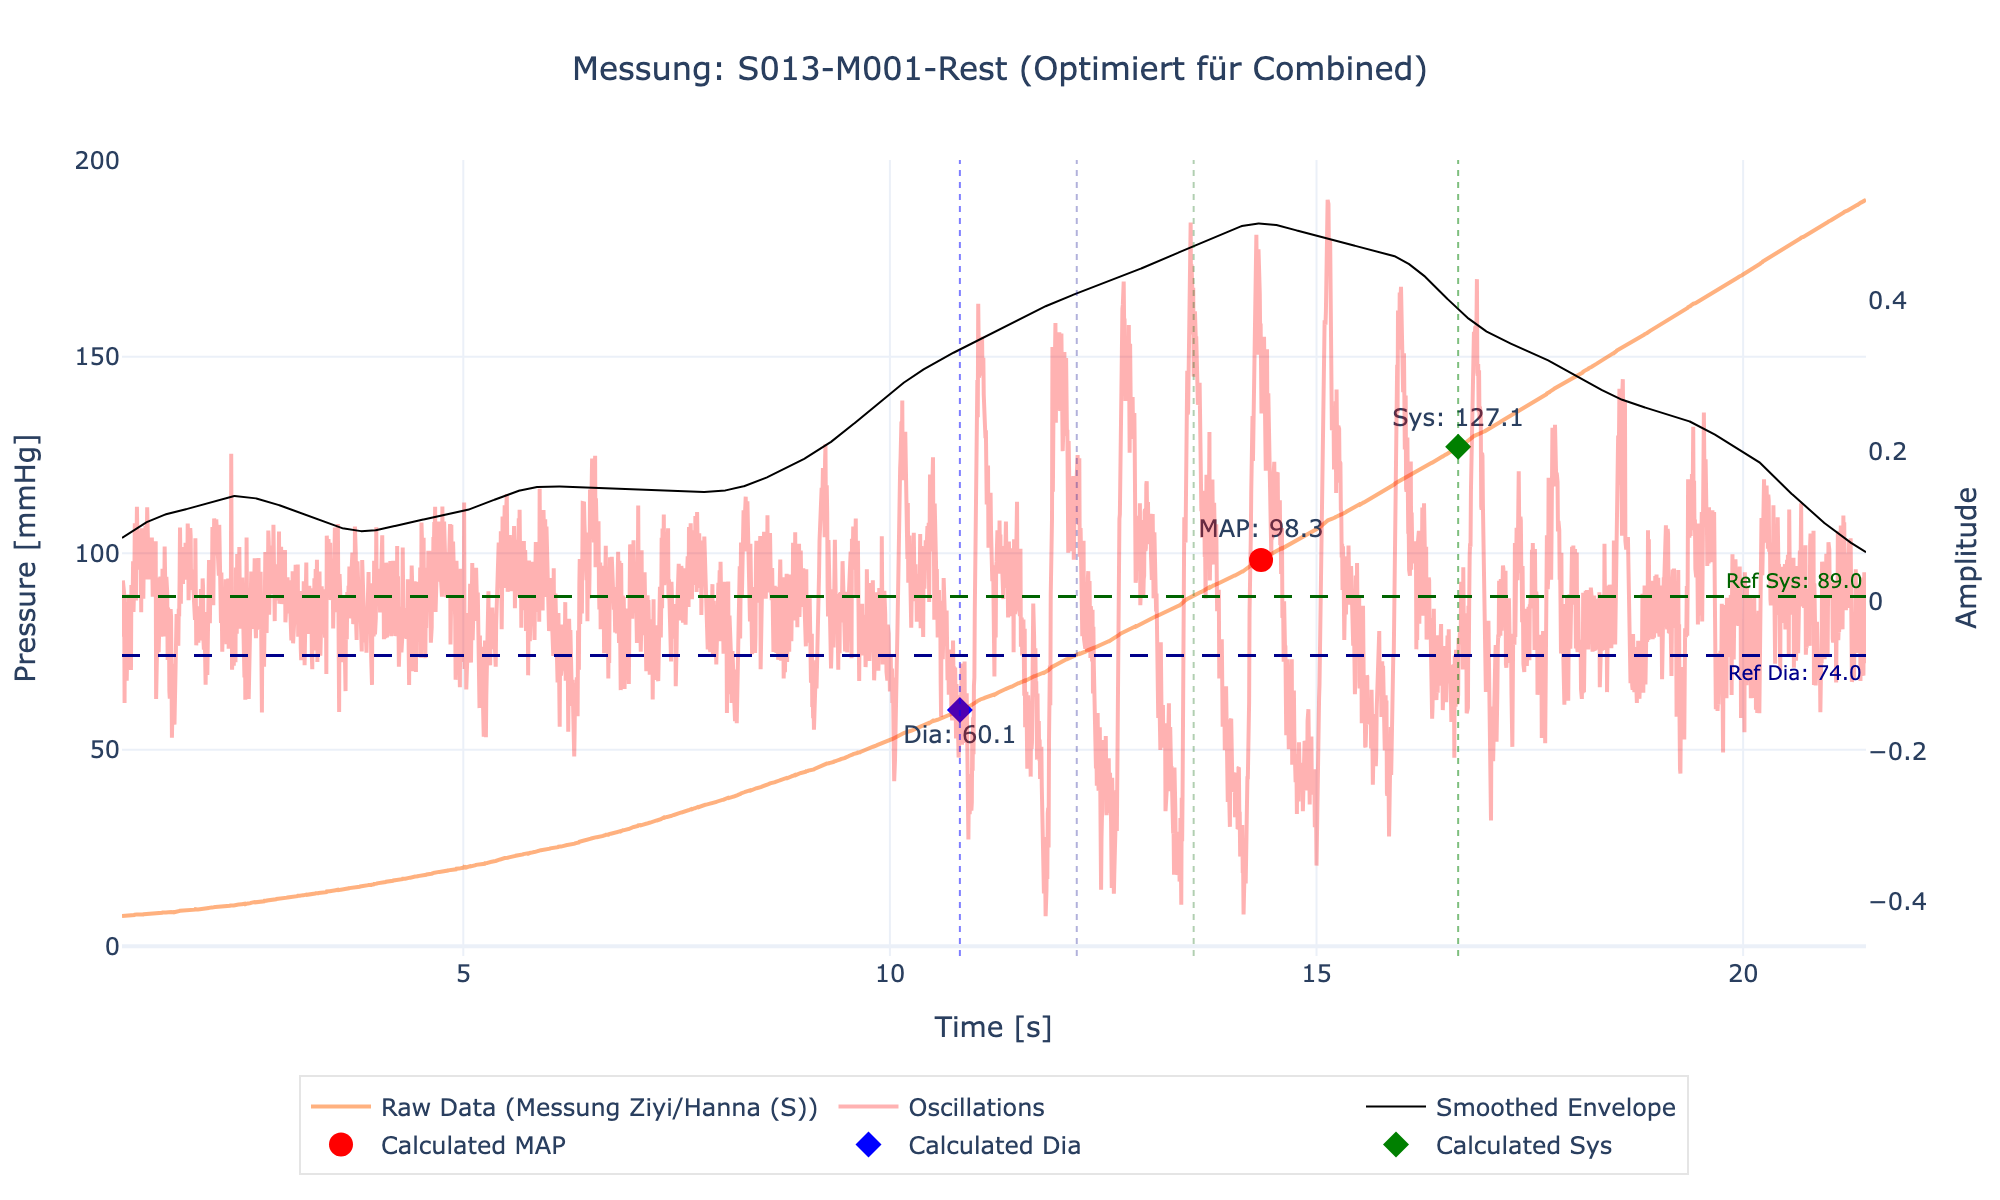
\includegraphics[width=\textwidth]{images/S013-M001-Rest_combined.png}
        \caption{Optimiert für Beurer und NAIS (Kombiniert)}
    \end{subfigure} \\
    \begin{subfigure}[b]{0.48\textwidth}
        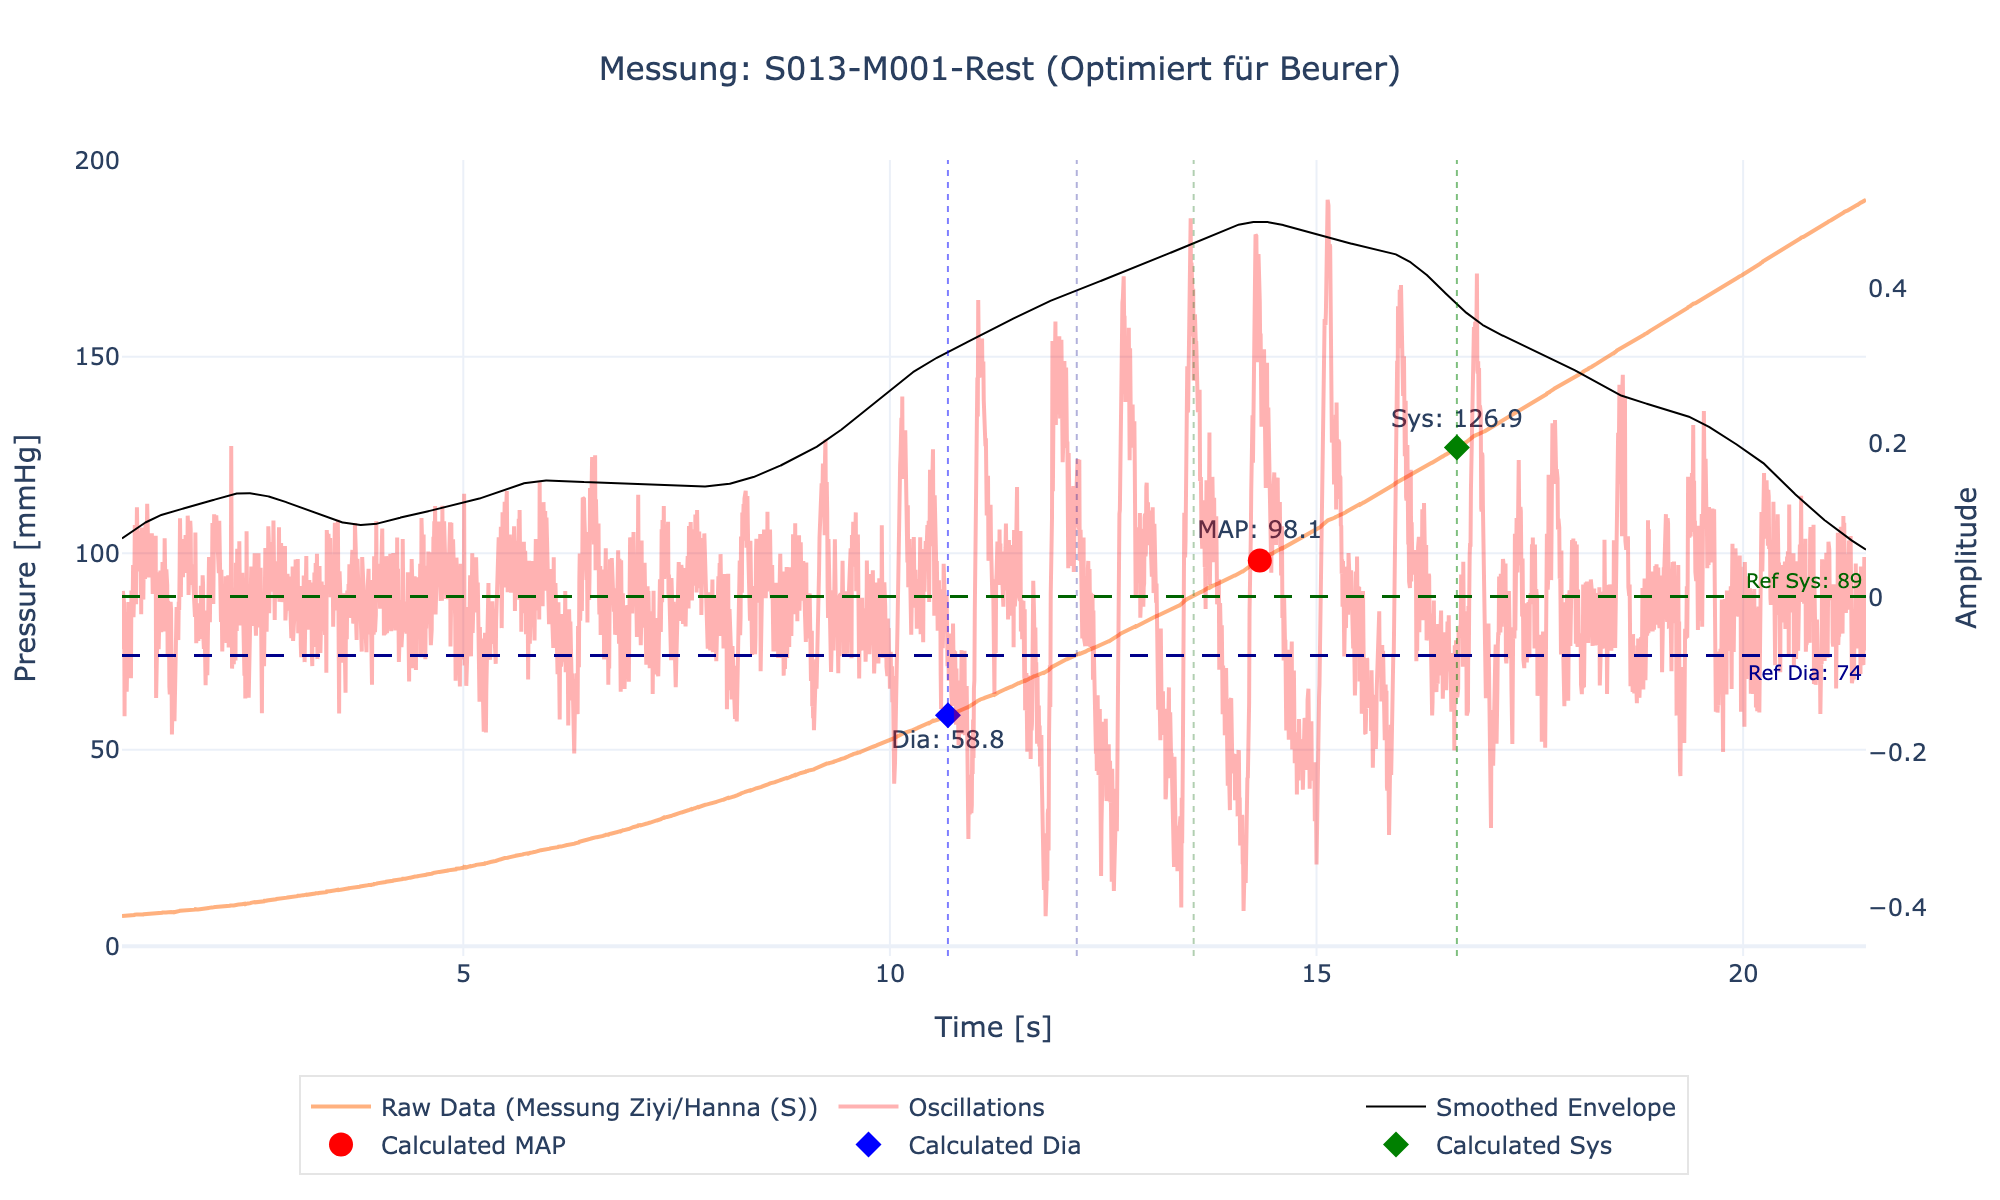
\includegraphics[width=\textwidth]{images/S013-M001-Rest_beurer.png}
        \caption{Optimiert für Beurer}
    \end{subfigure}
    \hfill
    \begin{subfigure}[b]{0.48\textwidth}
        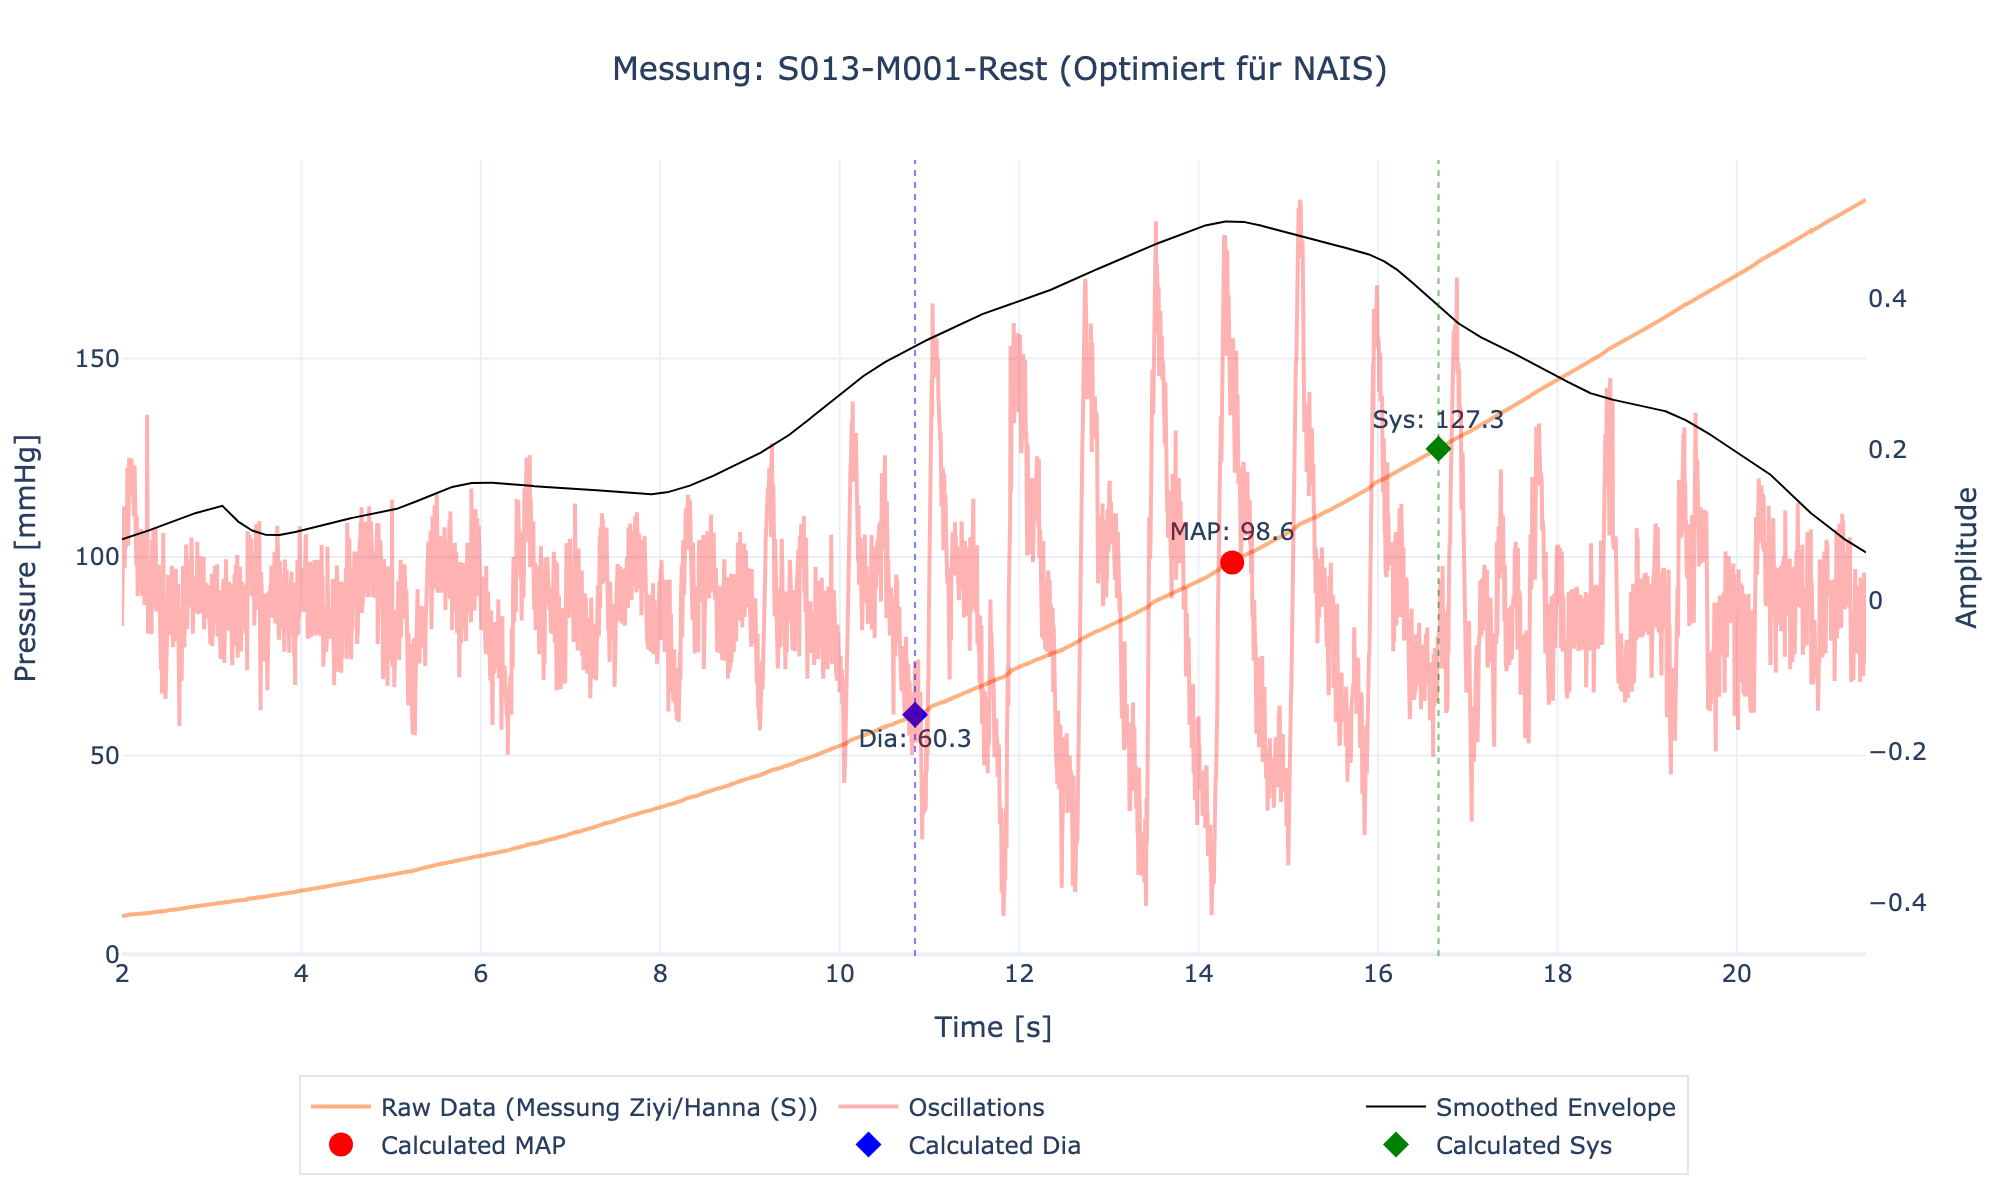
\includegraphics[width=\textwidth]{images/S013-M001-Rest_nais.png}
        \caption{Optimiert für NAIS}
    \end{subfigure}
    \caption{Einzelauswertung der Messung S013-M001-Rest mit verschiedenen Parametersätzen.}
\end{figure}
\newpage

\subsection*{Messung: S013-M002-Active}
\begin{figure}[H]
    \centering
    \begin{subfigure}[b]{0.8\textwidth}
        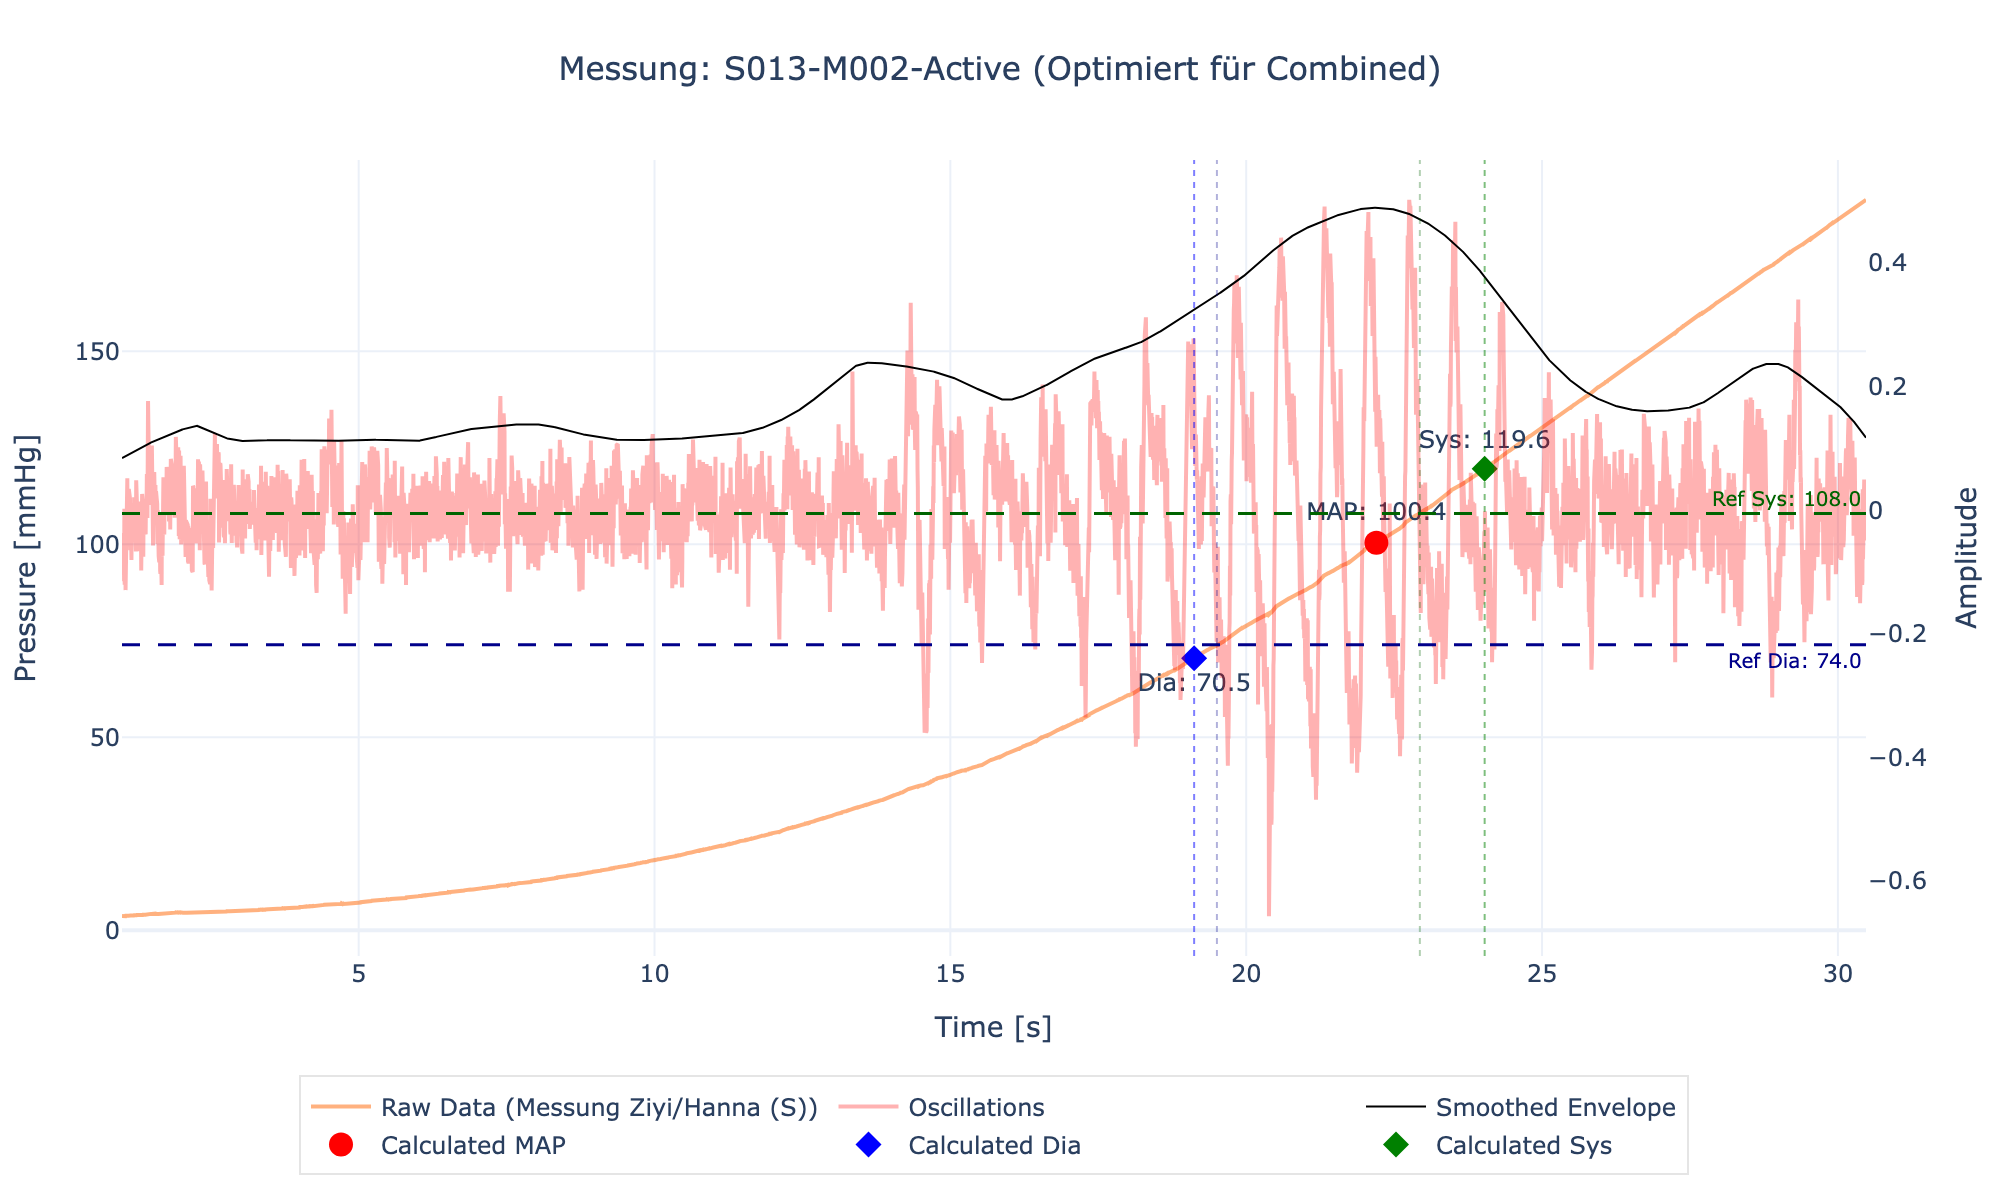
\includegraphics[width=\textwidth]{images/S013-M002-Active_combined.png}
        \caption{Optimiert für Beurer und NAIS (Kombiniert)}
    \end{subfigure} \\
    \begin{subfigure}[b]{0.48\textwidth}
        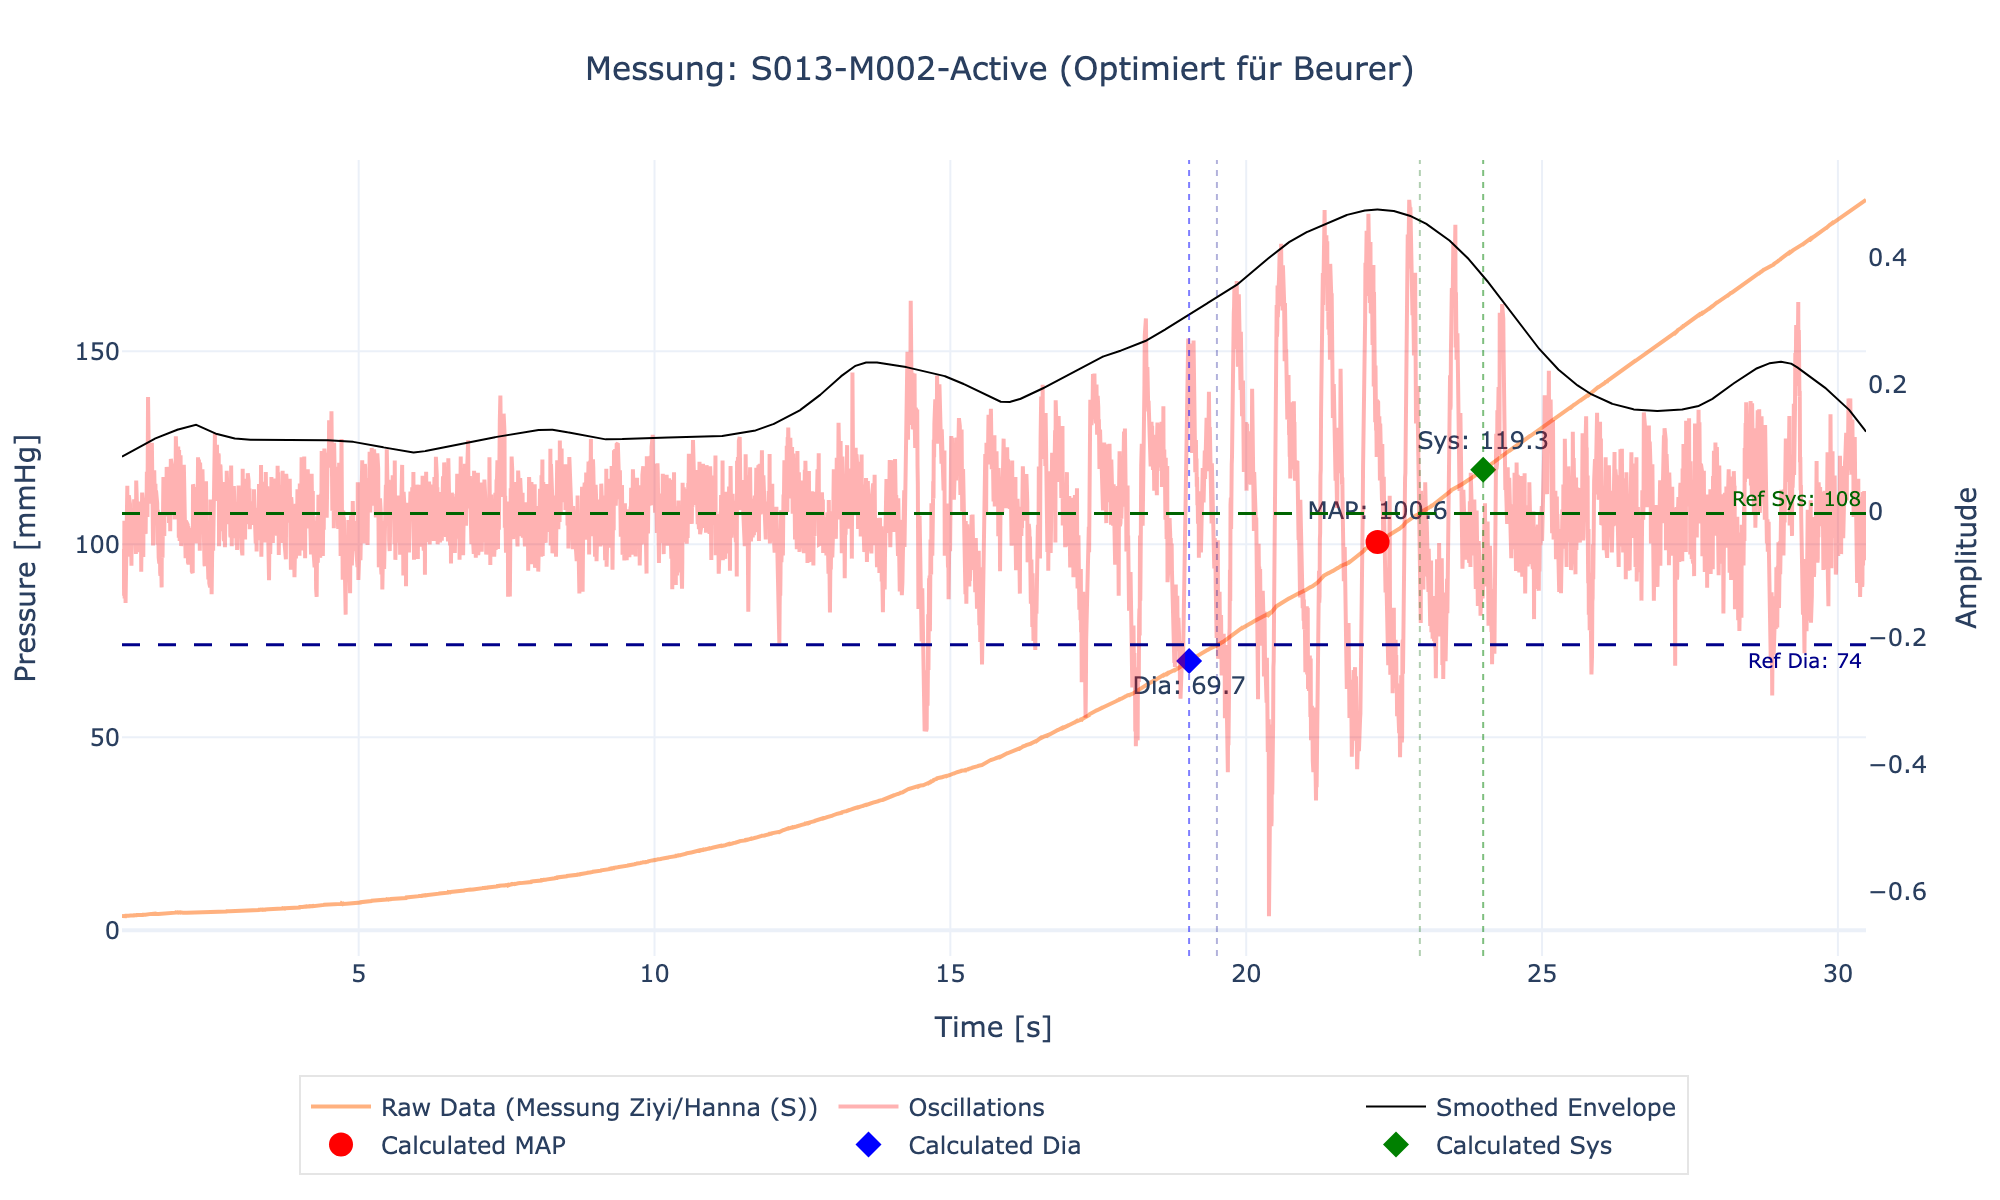
\includegraphics[width=\textwidth]{images/S013-M002-Active_beurer.png}
        \caption{Optimiert für Beurer}
    \end{subfigure}
    \hfill
    \begin{subfigure}[b]{0.48\textwidth}
        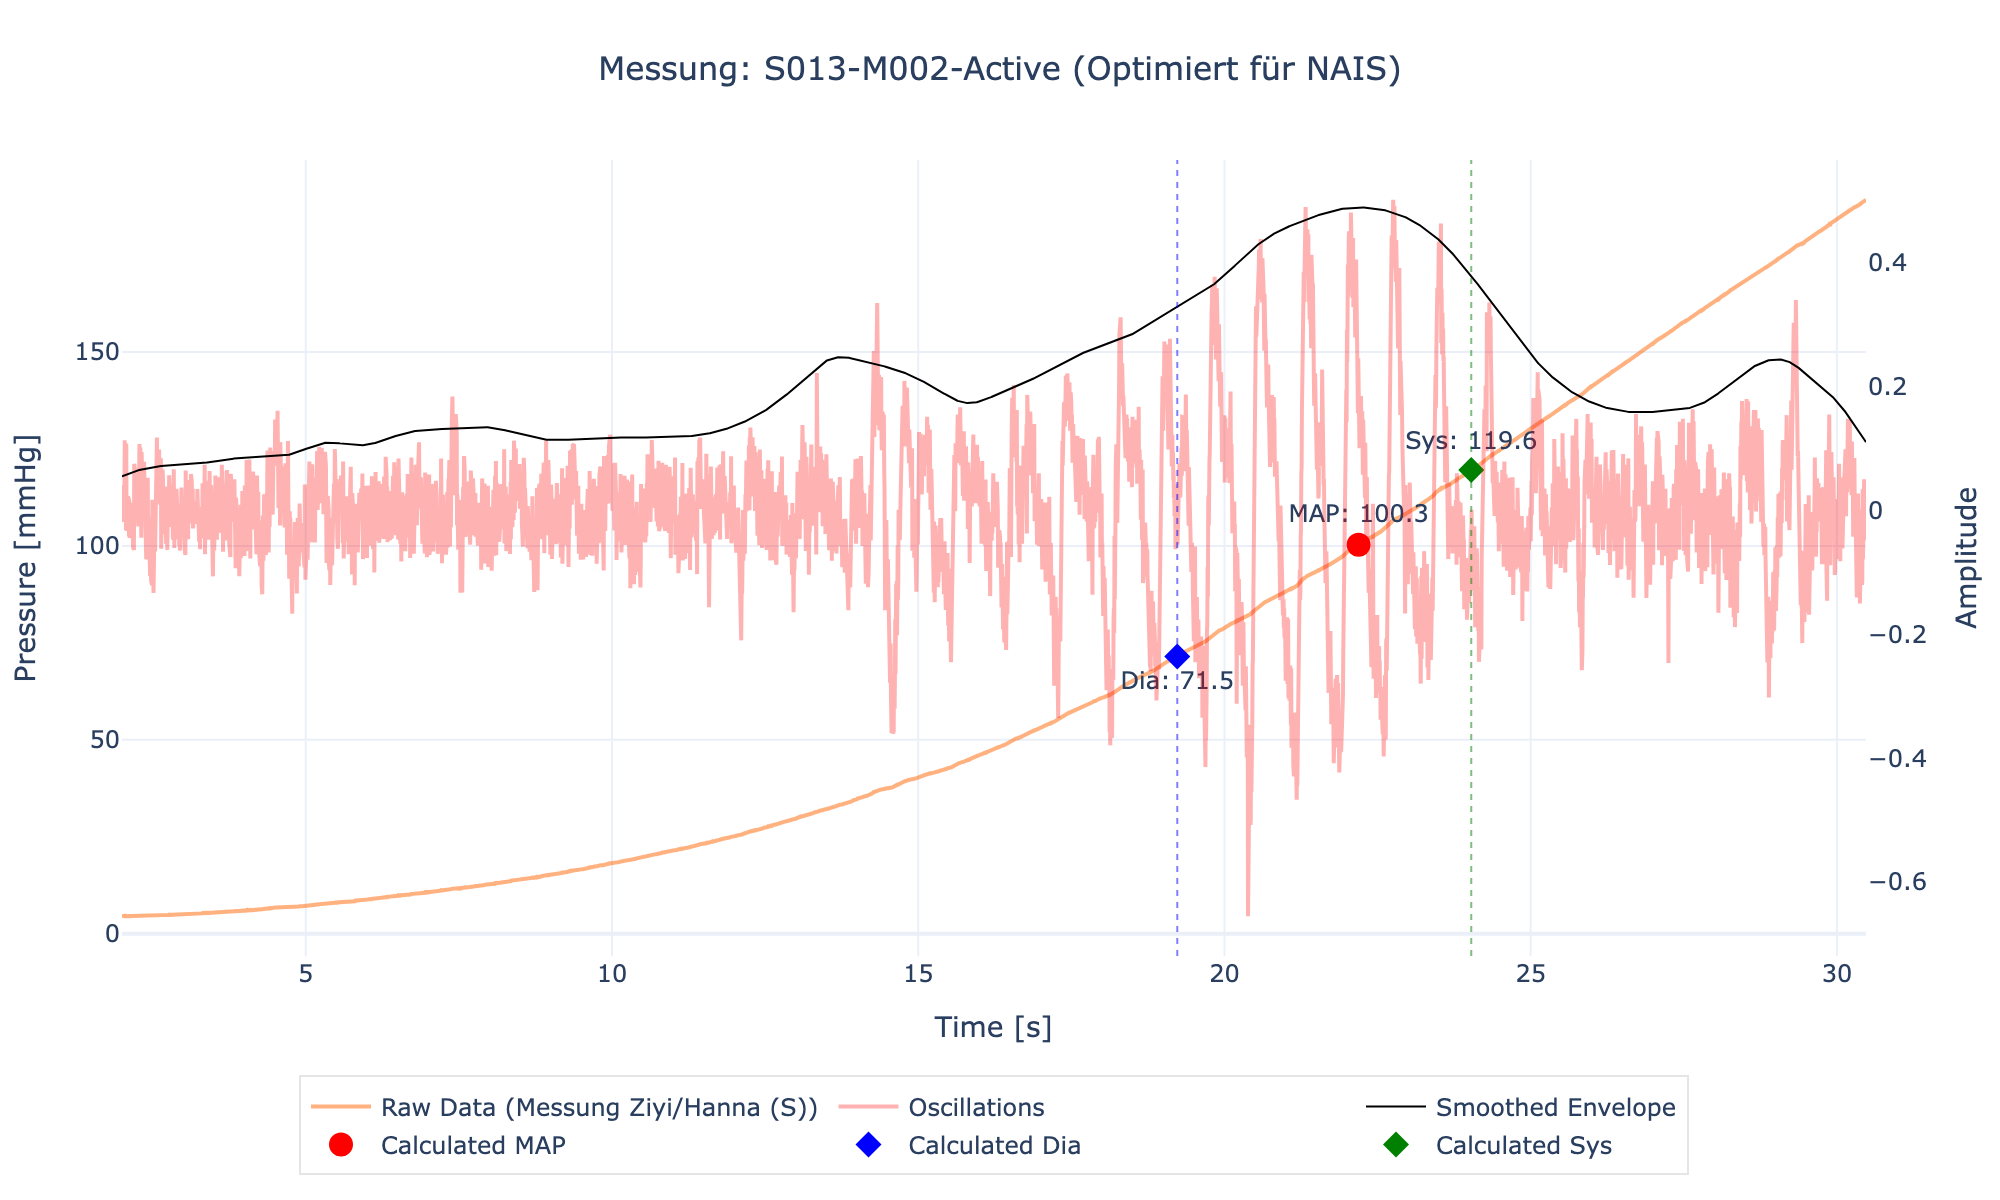
\includegraphics[width=\textwidth]{images/S013-M002-Active_nais.png}
        \caption{Optimiert für NAIS}
    \end{subfigure}
    \caption{Einzelauswertung der Messung S013-M002-Active mit verschiedenen Parametersätzen.}
\end{figure}
\newpage

